% Options for packages loaded elsewhere
\PassOptionsToPackage{unicode}{hyperref}
\PassOptionsToPackage{hyphens}{url}
\PassOptionsToPackage{dvipsnames,svgnames,x11names}{xcolor}
%
\documentclass[
  .7em,
  letterpaper,
  DIV=11,
  numbers=noendperiod]{scrartcl}

\usepackage{amsmath,amssymb}
\usepackage{lmodern}
\usepackage{iftex}
\ifPDFTeX
  \usepackage[T1]{fontenc}
  \usepackage[utf8]{inputenc}
  \usepackage{textcomp} % provide euro and other symbols
\else % if luatex or xetex
  \usepackage{unicode-math}
  \defaultfontfeatures{Scale=MatchLowercase}
  \defaultfontfeatures[\rmfamily]{Ligatures=TeX,Scale=1}
\fi
% Use upquote if available, for straight quotes in verbatim environments
\IfFileExists{upquote.sty}{\usepackage{upquote}}{}
\IfFileExists{microtype.sty}{% use microtype if available
  \usepackage[]{microtype}
  \UseMicrotypeSet[protrusion]{basicmath} % disable protrusion for tt fonts
}{}
\makeatletter
\@ifundefined{KOMAClassName}{% if non-KOMA class
  \IfFileExists{parskip.sty}{%
    \usepackage{parskip}
  }{% else
    \setlength{\parindent}{0pt}
    \setlength{\parskip}{6pt plus 2pt minus 1pt}}
}{% if KOMA class
  \KOMAoptions{parskip=half}}
\makeatother
\usepackage{xcolor}
\setlength{\emergencystretch}{3em} % prevent overfull lines
\setcounter{secnumdepth}{-\maxdimen} % remove section numbering
% Make \paragraph and \subparagraph free-standing
\ifx\paragraph\undefined\else
  \let\oldparagraph\paragraph
  \renewcommand{\paragraph}[1]{\oldparagraph{#1}\mbox{}}
\fi
\ifx\subparagraph\undefined\else
  \let\oldsubparagraph\subparagraph
  \renewcommand{\subparagraph}[1]{\oldsubparagraph{#1}\mbox{}}
\fi


\providecommand{\tightlist}{%
  \setlength{\itemsep}{0pt}\setlength{\parskip}{0pt}}\usepackage{longtable,booktabs,array}
\usepackage{calc} % for calculating minipage widths
% Correct order of tables after \paragraph or \subparagraph
\usepackage{etoolbox}
\makeatletter
\patchcmd\longtable{\par}{\if@noskipsec\mbox{}\fi\par}{}{}
\makeatother
% Allow footnotes in longtable head/foot
\IfFileExists{footnotehyper.sty}{\usepackage{footnotehyper}}{\usepackage{footnote}}
\makesavenoteenv{longtable}
\usepackage{graphicx}
\makeatletter
\def\maxwidth{\ifdim\Gin@nat@width>\linewidth\linewidth\else\Gin@nat@width\fi}
\def\maxheight{\ifdim\Gin@nat@height>\textheight\textheight\else\Gin@nat@height\fi}
\makeatother
% Scale images if necessary, so that they will not overflow the page
% margins by default, and it is still possible to overwrite the defaults
% using explicit options in \includegraphics[width, height, ...]{}
\setkeys{Gin}{width=\maxwidth,height=\maxheight,keepaspectratio}
% Set default figure placement to htbp
\makeatletter
\def\fps@figure{htbp}
\makeatother

\usepackage{booktabs}
\usepackage{longtable}
\usepackage{array}
\usepackage{multirow}
\usepackage{wrapfig}
\usepackage{float}
\usepackage{colortbl}
\usepackage{pdflscape}
\usepackage{tabu}
\usepackage{threeparttable}
\usepackage{threeparttablex}
\usepackage[normalem]{ulem}
\usepackage{makecell}
\usepackage{xcolor}
\usepackage{amsmath}
\usepackage{caption}
\KOMAoption{captions}{tableheading}
\makeatletter
\makeatother
\makeatletter
\makeatother
\makeatletter
\@ifpackageloaded{caption}{}{\usepackage{caption}}
\AtBeginDocument{%
\ifdefined\contentsname
  \renewcommand*\contentsname{Table of contents}
\else
  \newcommand\contentsname{Table of contents}
\fi
\ifdefined\listfigurename
  \renewcommand*\listfigurename{List of Figures}
\else
  \newcommand\listfigurename{List of Figures}
\fi
\ifdefined\listtablename
  \renewcommand*\listtablename{List of Tables}
\else
  \newcommand\listtablename{List of Tables}
\fi
\ifdefined\figurename
  \renewcommand*\figurename{Figure}
\else
  \newcommand\figurename{Figure}
\fi
\ifdefined\tablename
  \renewcommand*\tablename{Table}
\else
  \newcommand\tablename{Table}
\fi
}
\@ifpackageloaded{float}{}{\usepackage{float}}
\floatstyle{ruled}
\@ifundefined{c@chapter}{\newfloat{codelisting}{h}{lop}}{\newfloat{codelisting}{h}{lop}[chapter]}
\floatname{codelisting}{Listing}
\newcommand*\listoflistings{\listof{codelisting}{List of Listings}}
\makeatother
\makeatletter
\@ifpackageloaded{caption}{}{\usepackage{caption}}
\@ifpackageloaded{subcaption}{}{\usepackage{subcaption}}
\makeatother
\makeatletter
\@ifpackageloaded{tcolorbox}{}{\usepackage[many]{tcolorbox}}
\makeatother
\makeatletter
\@ifundefined{shadecolor}{\definecolor{shadecolor}{rgb}{.97, .97, .97}}
\makeatother
\makeatletter
\makeatother
\ifLuaTeX
  \usepackage{selnolig}  % disable illegal ligatures
\fi
\IfFileExists{bookmark.sty}{\usepackage{bookmark}}{\usepackage{hyperref}}
\IfFileExists{xurl.sty}{\usepackage{xurl}}{} % add URL line breaks if available
\urlstyle{same} % disable monospaced font for URLs
\hypersetup{
  pdftitle={Transformative Experiences and Counterfactuals},
  colorlinks=true,
  linkcolor={blue},
  filecolor={Maroon},
  citecolor={Blue},
  urlcolor={Blue},
  pdfcreator={LaTeX via pandoc}}

\title{Transformative Experiences and Counterfactuals}
\author{}
\date{}

\begin{document}
\maketitle
\ifdefined\Shaded\renewenvironment{Shaded}{\begin{tcolorbox}[interior hidden, breakable, frame hidden, borderline west={3pt}{0pt}{shadecolor}, boxrule=0pt, sharp corners, enhanced]}{\end{tcolorbox}}\fi

\hypertarget{should-i-become-a-vampire}{%
\section{Should I become a vampire?}\label{should-i-become-a-vampire}}

\hypertarget{should-i-move-to-a-different-country}{%
\section{Should I move to a different
country?}\label{should-i-move-to-a-different-country}}

\hypertarget{should-i-get-married}{%
\section{Should I get married?}\label{should-i-get-married}}

\hypertarget{should-i-have-a-child}{%
\section{Should I have a child?}\label{should-i-have-a-child}}

\hypertarget{should-i-take-this-job}{%
\section{Should I take this job?}\label{should-i-take-this-job}}

\hypertarget{transformative-experiences}{%
\subsection{Transformative
Experiences}\label{transformative-experiences}}

\begin{itemize}
\item
  Certain experiences we cannot know what experience will be like-- and
  it's consequences-- until we undergo the experience; an epistemic
  challenge
\item
  But also, many new/unknown experiences are personally transformative;
  will change your life and what it is like to be you
\end{itemize}

\hypertarget{epistemic-transformation}{%
\subsection{Epistemic Transformation}\label{epistemic-transformation}}

\begin{itemize}
\item
  Experiencing color for the first time can't be fully anticipated until
  it has been experienced; can't learn it by being told, have to
  experience it
\item
  Knowledge of what something is like and subjective point-of-view
  changes
\item
  Understand things in new way, gain new information
\item
  Depends on how much one already knows, and the experience involved
\item
  Stories, testimony, and theories aren't enough to teach you what it is
  like
\end{itemize}

\hypertarget{personal-transformation}{%
\subsection{Personal Transformation}\label{personal-transformation}}

\begin{itemize}
\item
  Some experiences can change your point of view, and by extension, your
  personal preferences, and perhaps even change the kind of person that
  you are or at least take yourself to be.
\item
  horrific physical attack, gaining a new sensory ability, having a
  traumatic accident, undergoing major surgery, winning an Olympic gold
  medal, participating in a revolution, having a religious conversion,
  having a child, experiencing the death of a parent, making a major
  scientific discovery, or experiencing the death of a child.
\end{itemize}

\hypertarget{two-forms-of-transformation}{%
\subsection{Two Forms of
Transformation}\label{two-forms-of-transformation}}

\begin{itemize}
\tightlist
\item
  Can be epistemically transformative, giving you new information in
  virtue of your experience.
\item
  Can be personally transformative, changing how you experience being
  who you are.
\item
  Some experiences may be epistemically transformative while not being
  personally transformative, like tasting a durian for the first time.
  Some experiences may be personally transformative without being
  epistemically transformative.
\end{itemize}

\hypertarget{both-epistemic-and-personally-transformative}{%
\subsection{Both Epistemic and Personally
Transformative}\label{both-epistemic-and-personally-transformative}}

\begin{itemize}
\tightlist
\item
  Having a transformative experience (both personal and epistemic)
  teaches you something new, something that you could not have known
  before having the experience, while also changing you as a person.
\item
  Choices involving transformative experiences, that is, your
  transformative choices, allow you to causally form what it will be
  like to be you in your future.
\end{itemize}

\hypertarget{autobiographical-memory-episodic-and-semantic}{%
\subsection{Autobiographical Memory: Episodic and
Semantic}\label{autobiographical-memory-episodic-and-semantic}}

\begin{itemize}
\item
  Endel Tulving distinguished between \emph{episodic} and
  \emph{semantic} memory (Tulving, 1983)
\item
  \textbf{Episodic Memory:} mental representation of the self as the
  agent or patient of some action, or as the stimulus or experiencer of
  some state

  \begin{itemize}
  \tightlist
  \item
    \emph{I gave a present to Lucy on her birthday} and \emph{Lucy made
    me very happy yesterday}
  \end{itemize}
\item
  \textbf{Semantic Memory:} is more generic, context-free knowledge
  about the world. Doesn't necessarily have to be in self-reference.

  \begin{itemize}
  \tightlist
  \item
    \emph{Apples are red, green, or yellow fruits} or \emph{I am a
    member of the middle class}, \emph{I am more than 6 feet tall}, and
    \emph{I am a neurotic extravert}.
  \end{itemize}
\end{itemize}

\hypertarget{associative-network-models-of-memory}{%
\subsection{Associative Network Models of
Memory}\label{associative-network-models-of-memory}}

\includegraphics{https://www.acrwebsite.org/volumes/v09/09046f01.gif}

\begin{center}\rule{0.5\linewidth}{0.5pt}\end{center}

\includegraphics{https://oxfordre.com/politics/doc/10.1093/acrefore/9780190228637.001.0001/acrefore-9780190228637-e-956-graphic-003-full.gif}

\begin{center}\rule{0.5\linewidth}{0.5pt}\end{center}

\includegraphics{https://www.researchgate.net/publication/28673820/figure/fig4/AS:669670675869717@1536673339737/Figure-One-Associative-network-example-The-intersection-between-the-networks-of-the.png}

\begin{center}\rule{0.5\linewidth}{0.5pt}\end{center}

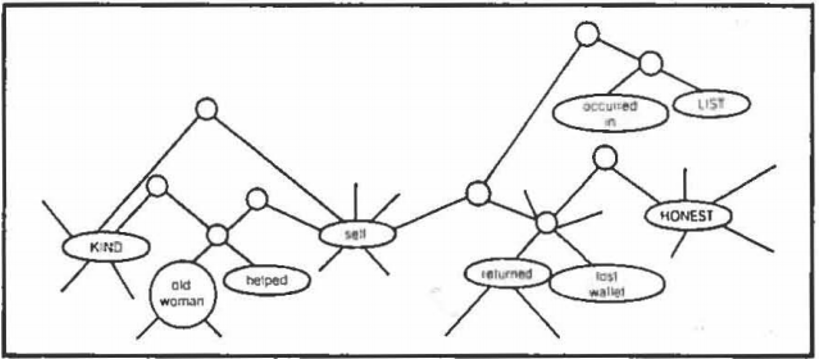
\includegraphics{images/Picture1.png}

\hypertarget{episodic-memories-as-a-causal-structure}{%
\subsection{Episodic Memories as a Causal
Structure}\label{episodic-memories-as-a-causal-structure}}

\begin{itemize}
\item
  Associativist models assume undirected relation
\item
  Also, to my knowledge, associativist models of self as memory have
  been primarily theoretical/verbal
\item
  Present works attempts to formally model episodic memories as
  causal/directed
\item
  Further, attempts to provide link between causal structure and
  ``transformation''
\end{itemize}

\hypertarget{hypotheses}{%
\section{Hypotheses}\label{hypotheses}}

\hypertarget{network-hypotheses}{%
\subsection{Network Hypotheses}\label{network-hypotheses}}

\begin{enumerate}
\def\labelenumi{\arabic{enumi}.}
\item
  H1: People will evaluate more positively, less negatively (i.e., more
  favorably) on memories with more downstram dependents.
\item
  H2: People will be more certain in memories with more downstream
  dependents.
\item
  H3: Memories with more dependents will be more clearly defined and
  accessible.
\item
  H4: Memories with more dependents will be farther back in time.
\end{enumerate}

\begin{center}\rule{0.5\linewidth}{0.5pt}\end{center}

\begin{enumerate}
\def\labelenumi{\arabic{enumi}.}
\setcounter{enumi}{4}
\item
  H5: Memories with more dependents will be more fundamental to how
  people see themselves, and if they were changed, would change the
  person.
\item
  H6: Memories with more dependents will be more important to the
  person.
\item
  H7: Time will be associated with the number of implications, such that
  experiences farther back in time will have caused more other
  experiences.
\item
  H8: How broad/specific an experience is may be associated with some
  perceptions or moderate various associations-- One example may be that
  broader memories will have more implications.
\end{enumerate}

\begin{center}\rule{0.5\linewidth}{0.5pt}\end{center}

\begin{enumerate}
\def\labelenumi{\arabic{enumi}.}
\setcounter{enumi}{8}
\item
  H9: People's self-report of retrospected emotions during an experience
  will be associated with how positively or negatively they perceive the
  experience.
\item
  H10: Memories with lower network constraint will be more
  differentiated. (pretty exploratory)
\item
  H11: People think more often about memories with more memories causing
  them
\end{enumerate}

\hypertarget{method}{%
\section{Method}\label{method}}

\begin{center}\rule{0.5\linewidth}{0.5pt}\end{center}

\begin{itemize}
\item
  Participants indicate up to 30 episodic experiences/personal memories

  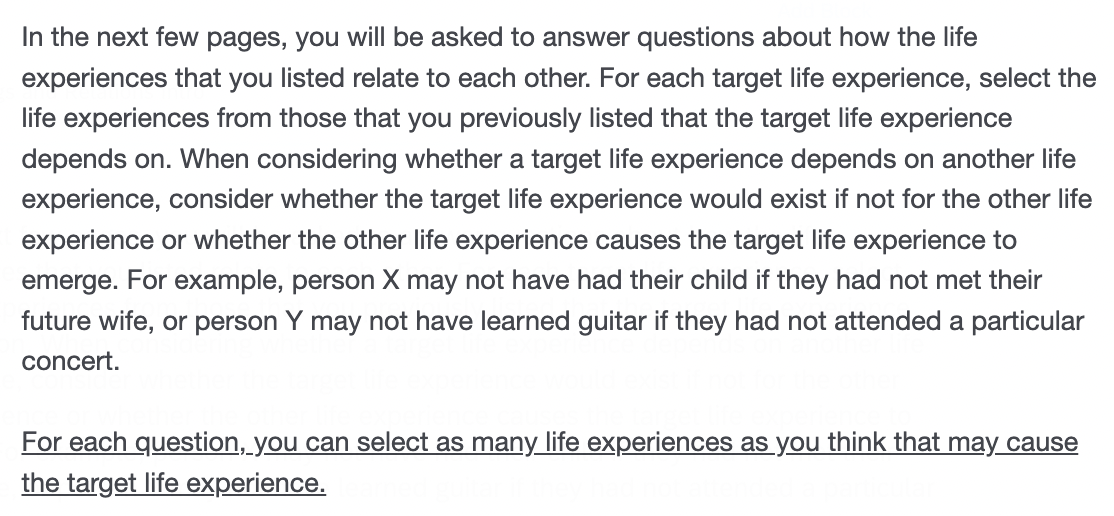
\includegraphics{images/Screen Shot 2023-01-27 at 10.23.58 PM.png}
\end{itemize}

\begin{center}\rule{0.5\linewidth}{0.5pt}\end{center}

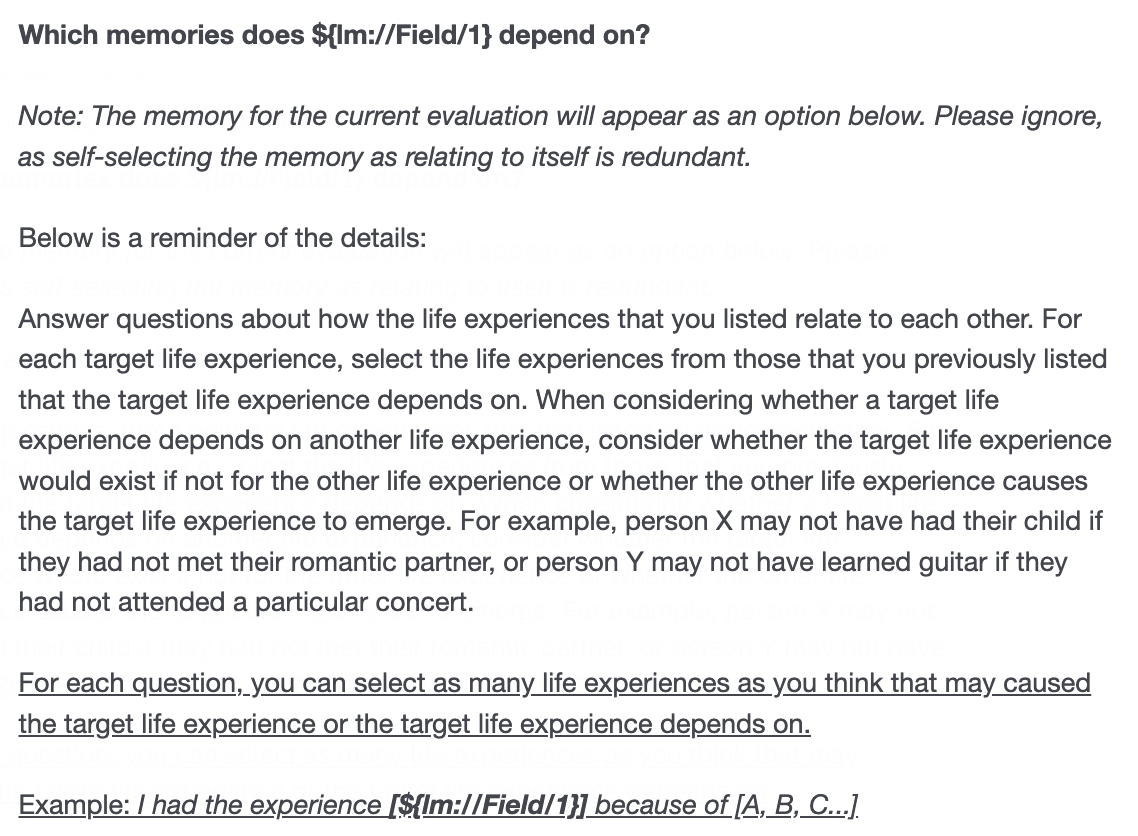
\includegraphics{images/Screen Shot 2023-01-27 at 10.25.35 PM.png}

\begin{center}\rule{0.5\linewidth}{0.5pt}\end{center}

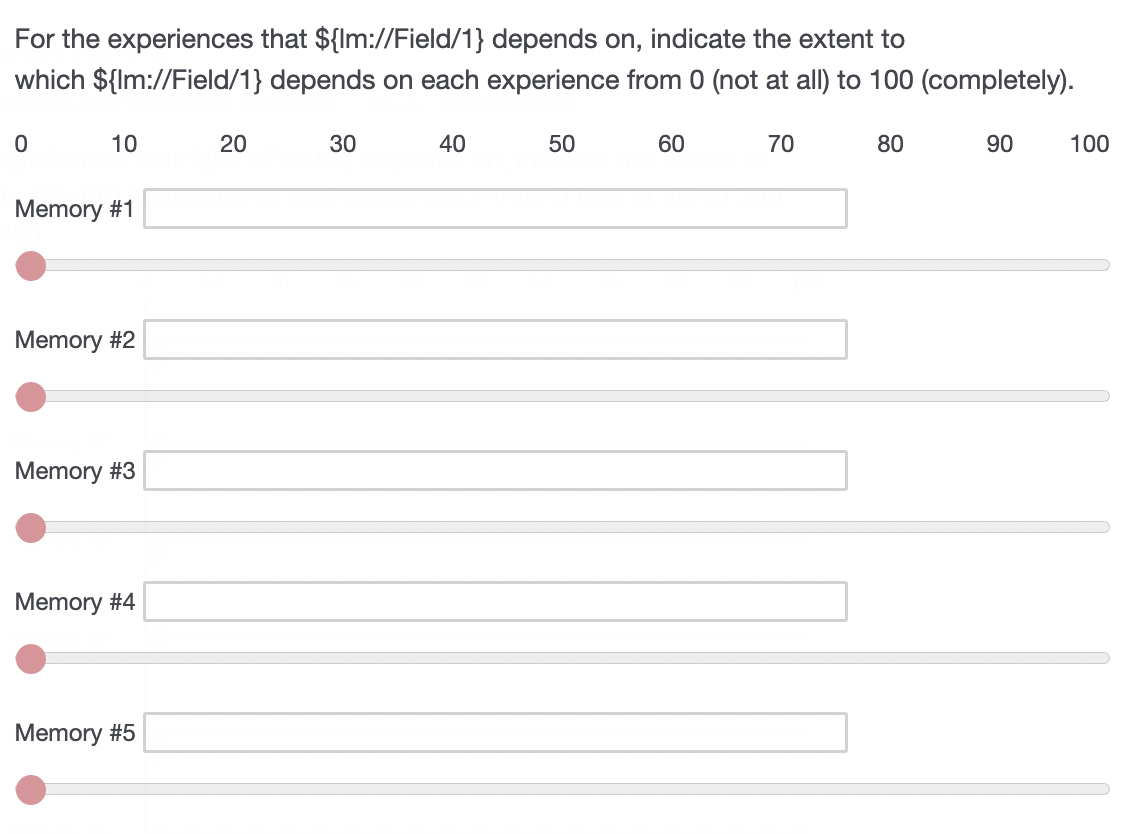
\includegraphics{images/Screen Shot 2023-01-27 at 10.29.31 PM.png}

\hypertarget{self-reported-measures}{%
\subsection{Self-Reported Measures}\label{self-reported-measures}}

\begin{itemize}
\tightlist
\item
  This experience is important to me.
\item
  The experience is important to others.
\item
  How do you feel about this experience? 0-100 {[}Positive/Negative{]}
\item
  During this experience, I felt\ldots{} {[}PANAS{]}
\item
  This experience is clearly-defined and easy to recall in my memory.
\item
  This experience is representative of who I am.
\item
  If I did not have this experience, I would be a fundamentally
  different person.
\item
  This experience changed me.
\item
  This experience is distinct and different from my other memories.
\item
  How certain do you feel about the details of this experience?
\item
  How often do you think about this experience?
\item
  How specific or broad was this experience?
\item
  To what extent does this experience involve yourself or others? 0-100
  {[}Self/Others{]}
\item
  How long ago was this experience?
\end{itemize}

\hypertarget{individual-differences}{%
\subsection{Individual Differences}\label{individual-differences}}

\begin{itemize}
\tightlist
\item
  Self-Esteem
\item
  Self-Concept Clarity
\item
  Need for Cognition
\item
  Dialectical Self
\item
  Depression
\item
  Interoception
\item
  Sense of Self
\item
  Self-Ambivalence
\item
  Dark Triad
\end{itemize}

\hypertarget{results}{%
\section{Results}\label{results}}

\hypertarget{wordcloud-of-frequently-used-words}{%
\subsection{Wordcloud of Frequently Used
Words}\label{wordcloud-of-frequently-used-words}}

\begin{verbatim}
Warning in tm_map.SimpleCorpus(., removeNumbers): transformation drops documents
\end{verbatim}

\begin{verbatim}
Warning in tm_map.SimpleCorpus(., removePunctuation): transformation drops
documents
\end{verbatim}

\begin{verbatim}
Warning in tm_map.SimpleCorpus(., stripWhitespace): transformation drops
documents
\end{verbatim}

\begin{verbatim}
Warning in tm_map.SimpleCorpus(docs, content_transformer(tolower)):
transformation drops documents
\end{verbatim}

\begin{verbatim}
Warning in tm_map.SimpleCorpus(docs, removeWords, stopwords("english")):
transformation drops documents
\end{verbatim}

\begin{verbatim}
Warning in tm_map.SimpleCorpus(docs, removeWords, c("the", "and")):
transformation drops documents
\end{verbatim}

\begin{verbatim}
Warning in wordcloud(words = df$word, freq = df$freq, min.freq = 1, max.words =
200, : mother could not be fit on page. It will not be plotted.
\end{verbatim}

\begin{verbatim}
Warning in wordcloud(words = df$word, freq = df$freq, min.freq = 1, max.words =
200, : crying could not be fit on page. It will not be plotted.
\end{verbatim}

\begin{verbatim}
Warning in wordcloud(words = df$word, freq = df$freq, min.freq = 1, max.words =
200, : another could not be fit on page. It will not be plotted.
\end{verbatim}

\begin{verbatim}
Warning in wordcloud(words = df$word, freq = df$freq, min.freq = 1, max.words =
200, : experiencing could not be fit on page. It will not be plotted.
\end{verbatim}

\begin{verbatim}
Warning in wordcloud(words = df$word, freq = df$freq, min.freq = 1, max.words =
200, : happy could not be fit on page. It will not be plotted.
\end{verbatim}

\begin{verbatim}
Warning in wordcloud(words = df$word, freq = df$freq, min.freq = 1, max.words =
200, : park could not be fit on page. It will not be plotted.
\end{verbatim}

\begin{verbatim}
Warning in wordcloud(words = df$word, freq = df$freq, min.freq = 1, max.words =
200, : finding could not be fit on page. It will not be plotted.
\end{verbatim}

\begin{verbatim}
Warning in wordcloud(words = df$word, freq = df$freq, min.freq = 1, max.words =
200, : thought could not be fit on page. It will not be plotted.
\end{verbatim}

\begin{verbatim}
Warning in wordcloud(words = df$word, freq = df$freq, min.freq = 1, max.words =
200, : room could not be fit on page. It will not be plotted.
\end{verbatim}

\begin{verbatim}
Warning in wordcloud(words = df$word, freq = df$freq, min.freq = 1, max.words =
200, : license could not be fit on page. It will not be plotted.
\end{verbatim}

\begin{verbatim}
Warning in wordcloud(words = df$word, freq = df$freq, min.freq = 1, max.words =
200, : christmas could not be fit on page. It will not be plotted.
\end{verbatim}

\begin{verbatim}
Warning in wordcloud(words = df$word, freq = df$freq, min.freq = 1, max.words =
200, : enough could not be fit on page. It will not be plotted.
\end{verbatim}

\begin{verbatim}
Warning in wordcloud(words = df$word, freq = df$freq, min.freq = 1, max.words =
200, : breaking could not be fit on page. It will not be plotted.
\end{verbatim}

\begin{verbatim}
Warning in wordcloud(words = df$word, freq = df$freq, min.freq = 1, max.words =
200, : reading could not be fit on page. It will not be plotted.
\end{verbatim}

\begin{verbatim}
Warning in wordcloud(words = df$word, freq = df$freq, min.freq = 1, max.words =
200, : however could not be fit on page. It will not be plotted.
\end{verbatim}

\begin{verbatim}
Warning in wordcloud(words = df$word, freq = df$freq, min.freq = 1, max.words =
200, : moment could not be fit on page. It will not be plotted.
\end{verbatim}

\begin{verbatim}
Warning in wordcloud(words = df$word, freq = df$freq, min.freq = 1, max.words =
200, : everyday could not be fit on page. It will not be plotted.
\end{verbatim}

\begin{verbatim}
Warning in wordcloud(words = df$word, freq = df$freq, min.freq = 1, max.words =
200, : wanted could not be fit on page. It will not be plotted.
\end{verbatim}

\begin{verbatim}
Warning in wordcloud(words = df$word, freq = df$freq, min.freq = 1, max.words =
200, : finally could not be fit on page. It will not be plotted.
\end{verbatim}

\begin{verbatim}
Warning in wordcloud(words = df$word, freq = df$freq, min.freq = 1, max.words =
200, : classes could not be fit on page. It will not be plotted.
\end{verbatim}

\begin{verbatim}
Warning in wordcloud(words = df$word, freq = df$freq, min.freq = 1, max.words =
200, : make could not be fit on page. It will not be plotted.
\end{verbatim}

\begin{verbatim}
Warning in wordcloud(words = df$word, freq = df$freq, min.freq = 1, max.words =
200, : phone could not be fit on page. It will not be plotted.
\end{verbatim}

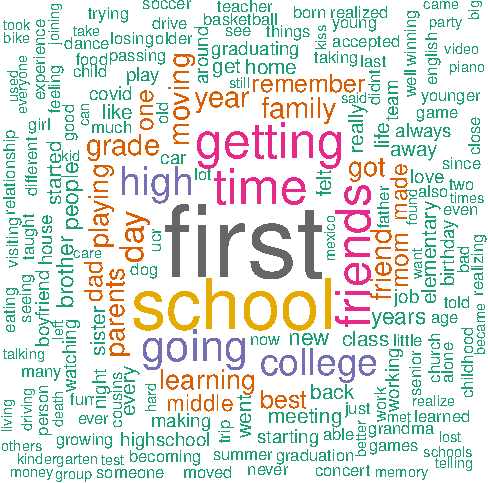
\includegraphics{EpMemNet_LabPres_htmldoc_files/figure-pdf/unnamed-chunk-2-1.pdf}

\hypertarget{table-of-experiences}{%
\subsection{Table of Experiences}\label{table-of-experiences}}

\begin{verbatim}
Warning: `as.tibble()` was deprecated in tibble 2.0.0.
Please use `as_tibble()` instead.
The signature and semantics have changed, see `?as_tibble`.
This warning is displayed once every 8 hours.
Call `lifecycle::last_lifecycle_warnings()` to see where this warning was generated.
\end{verbatim}

\begin{table}
\centering
\begin{tabular}{l}
\hline
value\\
\hline
My first day of Kindergarten, I cried and felt like I was extremely attached to my mom. I didn't want to let go\\
\hline
When I was little I always looked forward to my dad coming home and getting to hug him. He worked a lot because we needed money.\\
\hline
On my 7th birthday, I cried and I don't remember exactly why but I remember my family comforting me\\
\hline
When I was little me and my brothers would play forts, it's such a comforting memory because we were all little kids and that's all we were happy kids.\\
\hline
When my oldest brother got surgery on his appendix, it was a sad day\\
\hline
Going every Sunday morning to watch my brothers soccer games\\
\hline
When I was six, it was a Saturday afternoon and I remember making bracelets with my mom, it's such a heart-whelming memory\\
\hline
When I went to the Natural History Museum with my 5th grade class and we were running up this hill and it started raining but we were all just happy to be there\\
\hline
Making videos with my little brother around the house and just being funny and laughing is a pure memory I have\\
\hline
2010 Christmas, all my cousins were getting gifts but me and my brothers didn't get any because my dad didn't have enough money for gifts, it was a very sad thing as a kid but I understood my family was poor\\
\hline
I was in 8th grade, me and my best friend at the time were going back home and I remember we always laughed and had a good time, I remember this because it was a happy pure memory\\
\hline
Last 8th grade field trip to Medieval times, everyone in my 8th grade was super close to everyone and to see it was our last field trip before our lives changed going into high school will always stay with me\\
\hline
Crying a lot in front of the bathroom mirror when I was 14 because I felt so insecure about myself\\
\hline
When me and my family got evicted from home and we were homeless for months\\
\hline
My father giving me and brother a life lecture about not giving up in life no matter how hard things get\\
\hline
First day of High School, I felt out of place\\
\hline
Meeting my best friends that I made in high school\\
\hline
My 15th birthday which was the last day of my freshman year and when I also had my first kiss\\
\hline
March 13, 2020; life was never the same\\
\hline
The first day I began journalism to deal with my trauma and pain\\
\hline
When my grandma passed away, one truly painful memory\\
\hline
The first day of senior year, which was the day we came back to campus in person for the first time in over an year\\
\hline
Meeting Brandon, who was my first love\\
\hline
Brandon breaking my heart, it was my first heartbreak and it felt like my heart literally broke into pieces, one of the most hurting things I experienced\\
\hline
Gradnite, one last trip before my life was going to completely change once again\\
\hline
Graduation, such a surreal feeling\\
\hline
Move in day for college, saying goodbye to my family\\
\hline
My first communion\\
\hline
Meeting my siblings for the first time\\
\hline
Applying for college\\
\hline
Going to Vegas for the first time\\
\hline
Going to children's court\\
\hline
Getting on my first rollercoaster\\
\hline
My first kiss\\
\hline
High school graduation\\
\hline
High school prom\\
\hline
Meeting my boyfriend\\
\hline
When I lost my first tooth\\
\hline
First heartbreak\\
\hline
Eating delicious food\\
\hline
Visiting the family graveyard\\
\hline
Playing sports with my family\\
\hline
Playing video games with my friends\\
\hline
Writing short stories\\
\hline
Reading manga\\
\hline
Watching tv\\
\hline
Arguing online\\
\hline
My first episodic memory I can remember was when I got in trouble in kindergarten for getting in a fight with another kid. My mom did not hit me but was emotionally disappointed in me which forever changed me as a person in a way where I became more considerate of others.\\
\hline
My second episodic memory was when it was my fifth birthday and I had very little consciousness on what was going on, however in that moment I felt the greatest sense of satisfaction of obtaining gifts, cake, and a large gathering of people I knew, knowing it couldn't get any better than this.\\
\hline
My third memory happens to be in second grade when my best friend from kindergarten in which I have not seen since then came to visit me in class.This moment might have been the greatest satisfaction of having to see someone for a long time.\\
\hline
My fourth memory is the times I spent in 3rd to 5th grade with my best friend who had a disability speaking issue. This moment made me value those who have disabilities even more.\\
\hline
My fifth memory was the time I recieved my first pet cat around my middle school years who I still have today, and I appreciate and value her very much.\\
\hline
My sixth memory was when I visited my aunt in the hospital who have some sort of heart problem around 2010 I believe. I felt very scared thinking of what would become of her is she wasn't cured. (luckily she was and is doing good today)\\
\hline
My seventh memory was when I met my girlfriend in middle school. she has made me a more social person overall.\\
\hline
My eighth memory was when I reviewed my first piano as a gift from my father. I was self taught and value my talent to play it today\\
\hline
Taking a depression test during a checkup at the doctors.\\
\hline
My great grandma passing away.\\
\hline
Going to a field trip with my little sister and mom.\\
\hline
My trip to Florida.\\
\hline
Constantly moving homes during elementary school.\\
\hline
My aunt teaching me how to tie my shoes.\\
\hline
Getting lost at Disneyland.\\
\hline
Missing my first soccer game to go to Sea World.\\
\hline
Reading for the first time as a hobby.\\
\hline
Having someone close to me passing away.\\
\hline
Learning more about a subject I enjoy.\\
\hline
My dad taking me to trips.\\
\hline
My aunt talking me to different colleges.\\
\hline
My aunt and uncle talking about how I should go to college to earn a degree.\\
\hline
My mom telling me to get a better education cause she didn't\\
\hline
My grandparents helping me through out my childhood.\\
\hline
Me helping out my cousins when they seem they are in trouble.\\
\hline
At highschool when I recieved the news about Covid.\\
\hline
Getting accepted to colleges.\\
\hline
Growing up in the same town and learning so much about others and their situations\\
\hline
graduation high school and wannting to further my education.\\
\hline
The separation of my parents at a young age\\
\hline
meeting new people and figuring out if I like them or not\\
\hline
Getting in trouble for hanging out with the worng group.\\
\hline
Getting my High school Diploma\\
\hline
My first day of college\\
\hline
Going to my first concert\\
\hline
Turning 18/becoming an adult\\
\hline
Giving CPR to someone\\
\hline
My first job\\
\hline
going to cousin's house every weekend\\
\hline
grandma's house every weekend\\
\hline
house getting raided\\
\hline
dad and mom divorcing\\
\hline
dad picking me up from school everyday\\
\hline
going to a predominantly Mexican elementary school\\
\hline
1st period sophomore year of high school\\
\hline
going to my favorite english teacher in high school Mr. Perez's classroom during lunch\\
\hline
dad crying at the local park\\
\hline
watching mom and dad fight growing up\\
\hline
walking to dad's house after middle school\\
\hline
first dog dying\\
\hline
first heartbreak\\
\hline
when my father and I stopped speaking to each other\\
\hline
getting rejected from dream schools\\
\hline
grandma forgetting my name for the first time\\
\hline
first car accident\\
\hline
getting a brand new car\\
\hline
driving to best friend's house everyday in quarantine\\
\hline
quarantine walks\\
\hline
summer after high school\\
\hline
being the youngest of 5\\
\hline
finding out i'm actually the youngest of 6\\
\hline
my stepdad becoming my dad\\
\hline
grandma getting alzheimer's\\
\hline
dad being on house arrest\\
\hline
dad hitting mom for the first time\\
\hline
dad's overall abuse\\
\hline
getting my first job\\
\hline
being independent\\
\hline
being involved in softball for more than 6 years\\
\hline
I got accepted into all-stars softball after years of playing\\
\hline
Deciding that I couldn't play softball anymore because it made me anxious and not fun anymore\\
\hline
Freshman year of high school getting a new group of friends\\
\hline
March 13th 2020 when the shutdown first began\\
\hline
Getting accepted into college\\
\hline
Grad night having a fun night with my friends for like the last time\\
\hline
Graduation party where I realized that high school was really done\\
\hline
My 16th birthday party because it was the last time I really saw all my friends and family before the shutdown\\
\hline
When I broke both of my wrists at the same time and couldn't really do anything\\
\hline
when my younger sister was born\\
\hline
My avid banquet when I got to get my sash and got to spend time with my friends\\
\hline
feeling weird around friends because they wanted to drink\\
\hline
when the dodgers won the world series during a bad year\\
\hline
My 18th birthday going to Disneyland with my family\\
\hline
Singing in church\\
\hline
Moving to the US\\
\hline
First Day of Kindergarten\\
\hline
Birthday Celebration at my elementary school\\
\hline
Moved elementary school's\\
\hline
Hanging out with childhood best friends\\
\hline
Getting my first period\\
\hline
First day of Middle School\\
\hline
Becoming choir and band president\\
\hline
Going to knott's berry farm with friends\\
\hline
Promoting from Middle School\\
\hline
First day of high school\\
\hline
Met my longtime boyfriend\\
\hline
Began dating my boyfriend\\
\hline
first kiss\\
\hline
losing my virginity\\
\hline
worse depression, anxiety of my life, problems at home\\
\hline
COVID-19\\
\hline
Being at home with my family\\
\hline
Going back to school senior year\\
\hline
three year anniversary with my boyfriend\\
\hline
was gifted my first car\\
\hline
gradnite\\
\hline
graduation\\
\hline
summer break before college\\
\hline
college orientation\\
\hline
purchasing my own first car\\
\hline
first day of college\\
\hline
I found I was good at math\\
\hline
I got good grades\\
\hline
I did a lot of sports\\
\hline
I ate good food\\
\hline
I saw one piece\\
\hline
I decided to go to ucr\\
\hline
I started to procrastinate during covid\\
\hline
I am disappointed by the fact I am controlled by my fear.\\
\hline
Learning to Skate\\
\hline
Moving to Long Beach\\
\hline
Moved to a new school (multiple memories)\\
\hline
Parents divorcing\\
\hline
Watching my first Tarantino film\\
\hline
Separated parents\\
\hline
Absent father\\
\hline
First time meeting my baby brother\\
\hline
Visiting Mexico when I was younger\\
\hline
Mother always supporting me\\
\hline
Reunited both families at my Quince\\
\hline
Getting awards for my gpa\\
\hline
Being bullied for my skin color\\
\hline
Graduating high school\\
\hline
My dad becoming a single dad\\
\hline
Meeting my boyfriend\\
\hline
Play dates with my childhood best friend\\
\hline
Going to the beach with my grandma\\
\hline
Walking to school with nana\\
\hline
Playing with my brother\\
\hline
My sister being born\\
\hline
starting college\\
\hline
Grandma passing away\\
\hline
Learning how to cook with my mom\\
\hline
Talking about life with my dad while walking my dog at night\\
\hline
My first trip by myself\\
\hline
Learning how to knit with my grandmother\\
\hline
Moving in by myself for the first time; calling my new place ""home"" for the first time instead of calling my parent's house ""home""\\
\hline
My first day at work\\
\hline
Starting my first college assignment\\
\hline
Getting my first low grade on a college test\\
\hline
Discovering grief with my dog passing away\\
\hline
Going on my first vacation with my boyfriend\\
\hline
growing up in mexico as a full chinese descendant\\
\hline
speaking spanish throughout my whole life and people being suprised when they see me\\
\hline
moving around several times for elementary from to different countries\\
\hline
being bullied for my weight\\
\hline
playing family at preschool\\
\hline
leading youth group at church\\
\hline
piano lessons in 1-2 grade\\
\hline
church summer camp\\
\hline
fight with friend night before leaving taiwan\\
\hline
leaving school early to come to america\\
\hline
festival at church at night\\
\hline
Christmas performances for church, in taiwan and america\\
\hline
summer camp back at taiwan with american youths\\
\hline
not great interaction with some classmates first year\\
\hline
binge reading starting from 4th grade- read entire harry potter series\\
\hline
1st crush in 4th grade\\
\hline
mortifying christmas perfromance in 4th grade\\
\hline
promotion in 5th grade\\
\hline
psychology class in junior year learning about episodic memory\\
\hline
high school graduation\\
\hline
hearing covid news, school pausing\\
\hline
dealing with younger sister's suicide confession and coming out\\
\hline
first day of college at cpp\\
\hline
first day moving in apartment after transferring to ucr\\
\hline
getting a drive from a friend met in class\\
\hline
Moving out\\
\hline
Moving to California\\
\hline
Leaving High School\\
\hline
First major breakup\\
\hline
Dealing with SA\\
\hline
Deciding to go to UCR\\
\hline
Being hospitalized\\
\hline
Coming out\\
\hline
Defending myself in a toxic work environment\\
\hline
Taking my first psychology class\\
\hline
Realizing what actually happened in my childhood\\
\hline
Making the wrong decision with a friend\\
\hline
Christmas eve and Christmas day 2017\\
\hline
Life threatening sickness with my stomach\\
\hline
Getting in trouble with the authorities\\
\hline
getting put into counseling because of my grades\\
\hline
being cured, and finally having a painless life again\\
\hline
getting out of counseling because of my overall change in academics, and performances.\\
\hline
Getting an academic grade in 8th grade because of my grades turning around\\
\hline
Entering High School with the thought of a new beginning\\
\hline
Joining  my first sport Wrestling\\
\hline
Graduating High school in the honor role\\
\hline
Being accepted into 6 Universities\\
\hline
Choosing UCR as my final Decision\\
\hline
Completing my first week in UCR\\
\hline
my kindergarten best friend moving away\\
\hline
meeting my baby sister\\
\hline
the first day of middle school\\
\hline
playing at the park with my cousins\\
\hline
getting sand dumped in my hair by my cousin at age 4\\
\hline
graduating 8th grade\\
\hline
first band camp\\
\hline
first band competiton\\
\hline
YALE summer camp\\
\hline
getting accepted to college\\
\hline
covid at the end of senior year\\
\hline
moving into dorms\\
\hline
moving into an apartment\\
\hline
my college friends\\
\hline
Becoming captain of my high school xc team.\\
\hline
Deciding to quit playing soccer.\\
\hline
Running my first college xc race.\\
\hline
Receiving college acceptance letters.\\
\hline
Graduating high school.\\
\hline
Receiving most valuable athlete in high school.\\
\hline
Being MVP of my high school soccer team.\\
\hline
Overcoming mental health issues.\\
\hline
Going to a Bad Bunny concert.\\
\hline
Painting in my room during covid.\\
\hline
Doing an internship over the summer.\\
\hline
Passing my drivers test.\\
\hline
Moving into my college dorm.\\
\hline
Asking a girl who had no friends to hang out with me.\\
\hline
Helping my cousin when her dog go sprayed by a skunk.\\
\hline
Learning about the gaming community.\\
\hline
Moving to the untied stated\\
\hline
High school Graduation\\
\hline
Getting married\\
\hline
First child born\\
\hline
Second child born\\
\hline
getting a divorce\\
\hline
moving to Arizona\\
\hline
working at the airport\\
\hline
getting remarried\\
\hline
having marriage problems\\
\hline
birthing my third chid\\
\hline
my fourth child\\
\hline
my fifth child birth\\
\hline
my twins borns\\
\hline
my pregnancy with the twins\\
\hline
my illness during pregnancy\\
\hline
my separation from my husband\\
\hline
going back to school\\
\hline
covid\\
\hline
daughter missing\\
\hline
finding my daughter\\
\hline
daughter wedding\\
\hline
being selected as the commencement speaker\\
\hline
giving my commencement speech\\
\hline
my acceptance letters to the universities\\
\hline
graduating with honors\\
\hline
first day UCR\\
\hline
working for college Corp\\
\hline
filling for a divorce\\
\hline
dating after 18 years\\
\hline
The time I impaled my arm and got stiches\\
\hline
Growing up and hearing stories from my parents of what they had to go through\\
\hline
Not being able to see my mom because she worked when I got back from school when in elementary\\
\hline
My dad always giving effort to be around us and having fun even though he would get home from long shifts of work\\
\hline
My siblings doing random things for fun\\
\hline
Many of my relatives passing away at young ages\\
\hline
Sitting in the living room crying\\
\hline
My parents struggling and working to provide for us\\
\hline
My parents separated when I was 3\\
\hline
My great grandpa taught me how to ride a bike\\
\hline
I rolled my sister's bike in a cowpie in the rain\\
\hline
Hit a granny shot in a basketball game and went to a buffet after\\
\hline
Made 3 free throws to win a Varsity basketball game\\
\hline
Sneaking into my friends house at night\\
\hline
Skating around town at 3 am\\
\hline
Attempting self harm 4 years ago and my dad came to my house\\
\hline
Sitting outside my ex's house to talk through our problems at 12 am\\
\hline
Breaking the window to the laundry room with a tennis ball\\
\hline
My brother farted in my sister's face with his pants down when he was 9\\
\hline
My dad would jump on my bed and wake me up when it was my birthday\\
\hline
I attended junior college classes with my dad in 1st grade\\
\hline
Taking my ex stargazing at 4 am\\
\hline
Making my promposal for my ex with my friend\\
\hline
I was surprised to realize that some of my friends truly believed in God and that made me question religion twice. However, I still don't believe in God, but now I understand why people do.\\
\hline
This girl I liked, I knew she liked someone else, and that completely changed me.\\
\hline
After interacting with more and more liberal media, I have found myself shifting more and more towards conservatism.\\
\hline
Moving back to the US and also moving from the US were both impactful experiences.\\
\hline
When i graduated high school\\
\hline
When I watched anime with my siblings when i was younger\\
\hline
Eating with my family together and laughing with them\\
\hline
When i failed my first class\\
\hline
When I first started listening to music with my dad\\
\hline
When I first learned to drive\\
\hline
When I left Colorado and moved out to California\\
\hline
The last month or two of my first year in high school\\
\hline
When my little brother was born\\
\hline
My first performance\\
\hline
My first audition\\
\hline
My first acting workshop\\
\hline
Getting my first sketchbook\\
\hline
My first day of elementary school\\
\hline
Bringing my first dog home\\
\hline
Bringing my second dog home\\
\hline
Learning to drive\\
\hline
Learning to ride a bike\\
\hline
Moving to college\\
\hline
Working as an RBT\\
\hline
Training in Boxing\\
\hline
Spending time with family\\
\hline
Taking the iniative to try new things\\
\hline
The death of a close friend\\
\hline
Going to anime conventions\\
\hline
Going to many concerts\\
\hline
Receiving my UCR acceptance letter\\
\hline
Traveling to another state and country\\
\hline
Signing up on social media\\
\hline
Los Alamitos\\
\hline
Covid\\
\hline
Church\\
\hline
San Diego\\
\hline
Oxford\\
\hline
Going early morning lake fishing with my father when I was 9 years old\\
\hline
My grandfather reading me ""where the wild things are"" before I went to bed\\
\hline
my dad and uncle engaging in an argument due to my uncle being drunk and difficult in front of my grandmother\\
\hline
me and my little brother climbing an oak tree in my backyard\\
\hline
early morning birdwatching with my brother\\
\hline
spending the days surrounding new years with my aunt and cousins\\
\hline
visiting an art museum with my parents\\
\hline
my 14th birthday party with my grandmother, parents, and siblings\\
\hline
playing my first video game\\
\hline
taking music classes\\
\hline
attending my first concert\\
\hline
adapting to my disabilities at a young age\\
\hline
countless lectures my parents would give me as a kid\\
\hline
school and everything about it, especially throughout elementary\\
\hline
competing against other people through sports or academics\\
\hline
countless adventures with my good friends\\
\hline
When one of the people who were renting one of the rooms in my house started yelling at me at 5:30 in the morning when I was going to swimming class\\
\hline
When a cat pooped on my couch and I found out early in the morning before swim practice\\
\hline
When my parents got mad at me for breaking a piece of glass\\
\hline
Convincing my dad to get me a speed racer novel that I never read, I thought the title looked cool\\
\hline
My art teacher giving me a C for an anatomy assignment but giving another kid who drew the head way too big an A\\
\hline
Losing my very first swimming race.\\
\hline
Diving for the first time and bellyflopping onto the pool\\
\hline
Getting my first kiss outside my house\\
\hline
First time going to Disneyland\\
\hline
First time trying In and Out\\
\hline
Getting my first dog\\
\hline
Loosing my first dog\\
\hline
Becoming a tia\\
\hline
Promoting 8th grade\\
\hline
My first day of high school\\
\hline
My last day of high school\\
\hline
Graduating High school\\
\hline
Going to Prom\\
\hline
Meeting my first friend\\
\hline
Learning how to drive\\
\hline
Getting License\\
\hline
Moving out of my house\\
\hline
Moving into my dorm\\
\hline
flying in an airplane for the first time\\
\hline
going to Mexico for the first time\\
\hline
Experiencing a car accident\\
\hline
Getting my first car\\
\hline
Learning how to do lash extententions\\
\hline
my first job\\
\hline
becoming a cheerleader\\
\hline
getting accepted to UCR\\
\hline
going to my first party\\
\hline
First time I went to Sri Lanka\\
\hline
First time I drove a car\\
\hline
Running into a friend I haven't seen in a while\\
\hline
Enjoying some unexpected time alone more compared to going out all the time with friends\\
\hline
Realizing I've mastered a difficult skill, specifically Algebra which used to be difficult until I put in the practice and effort\\
\hline
The death of a loved one- made me value people more and the time I have left with everyone around me\\
\hline
Avalanche - natural disaster, made me be more careful around terrain I'm not familiar with\\
\hline
Getting appendicitis - made me create more healthy habits, watch what I eat, be more hygienic\\
\hline
First time a child hugged me (my baby cousin) - made me feel warm and loved\\
\hline
Falling in love for the first time - realizing the extent to how much I could care about someone who wasn't family\\
\hline
Getting my heart broken/rejected - realizing how much it hurts, experiencing a different type of sadness, but thankful I'm able to experience that much sadness over a relationship\\
\hline
Entering college - scared but also eager after seeing how large the campus was and the workload and amount of learning needed to be successful\\
\hline
Going out on solo trips by myself - made me realize I don't need to go out places with friends all the time to enjoy things, can enjoy me time, time alone is therapy\\
\hline
First real/best/good friend - made me have a different perspective of life, taught me things I didn't know about myself and the world, shaped my life for the better\\
\hline
making varsity waterpolo and tennis\\
\hline
learning to ride a bike\\
\hline
learning to drive\\
\hline
getting into UCR\\
\hline
passing all my AP classes\\
\hline
my parents arguing\\
\hline
my brother and sister in the hospital at the same time\\
\hline
my parents separating for a little\\
\hline
my sister going in and out of the hospital\\
\hline
my sister passing away\\
\hline
my first love\\
\hline
my sister helping me with everything\\
\hline
my dad becoming my friend\\
\hline
the feeling of becoming an adult\\
\hline
when I got my first car\\
\hline
when I got my first job\\
\hline
the time I balanced 2 jobs and sports, and school\\
\hline
when I re did my room all by myself\\
\hline
putting together legos with my family\\
\hline
eating dinner talking about our day with my family\\
\hline
when we went to disneyworld for make a wish\\
\hline
train park\\
\hline
stuck in elevator\\
\hline
trying ice cream for the first time\\
\hline
eating biriyani\\
\hline
getting my chin split open\\
\hline
getting hit on my head with a guitar\\
\hline
watching mostober\\
\hline
watching spongebob\\
\hline
listening to one direction\\
\hline
one direction concert\\
\hline
roy woods concert\\
\hline
post malone concert\\
\hline
hiking in hawaii\\
\hline
working at express\\
\hline
working at yumi yogurt\\
\hline
working at sweet rendezvous\\
\hline
going to the city SF\\
\hline
riding the cal train\\
\hline
going to turkey\\
\hline
going on a hot air balloon\\
\hline
going to dubai\\
\hline
going to pakistan\\
\hline
going to italy\\
\hline
riding a gondola\\
\hline
going to canada\\
\hline
watching corpse bride\\
\hline
watching titanic for the first time\\
\hline
meeting the captain of Pakistan's cricket team\\
\hline
visiting family in pakistan\\
\hline
going on a rollercoaster for the first time\\
\hline
commucate with other people\\
\hline
listen to my parent when they are talking\\
\hline
take to my workmate\\
\hline
handout with my friends\\
\hline
My sister being born\\
\hline
Taking a trip to Thailand\\
\hline
Taking a trip to Latvia\\
\hline
Taking a trip to Mexico\\
\hline
My parents telling me they are getting divorced\\
\hline
One on one conversations with my father\\
\hline
One on one conversations with my mother\\
\hline
One on one conversations with my grandmothers\\
\hline
One on one conversations with my grandfathers\\
\hline
Standing up for my religious heritage\\
\hline
Standing up for my cultural heritage\\
\hline
My grandfather passing away\\
\hline
Skiing with my father\\
\hline
Playing soccer with my friends\\
\hline
Playing basketball with my friends\\
\hline
Learning from my elementary teachers the importance of treating others the way you want to be treated\\
\hline
Having personal conversations with my sister\\
\hline
Having personal conversations with my two closest friends\\
\hline
Graduating high school\\
\hline
Getting made fun of\\
\hline
Talking with my father about the principles of being a strong man\\
\hline
Talking with my mother about the importance of being selfless\\
\hline
Celebrated Chinese Lunar new year with friends in Hong Kong\\
\hline
Went to Japan with family for several times\\
\hline
Went to Macau in 2020\\
\hline
Participated Leadership program with friends in 2019\\
\hline
Went to kindergarten in Cerrtios\\
\hline
Learned piano for 8 years\\
\hline
Went to Boracay with family\\
\hline
Went to Guam with family twice\\
\hline
Went to Philippine with friends twice\\
\hline
Took yoga class with friends\\
\hline
Went to night markets with friend\\
\hline
Took Mexico Cruise when I was little\\
\hline
Watched the Phantom of the Opera\\
\hline
Went to Time Square twice\\
\hline
Visited the Central Park Tower and watched 131st floor view\\
\hline
Went to Bali Island with family\\
\hline
Wen to a concert with friends\\
\hline
Celebrated 18th birthday with friends\\
\hline
Lived in Boston University dormitory with friends\\
\hline
Visited Harvard and MIT\\
\hline
Going to summer camp by myself (11)\\
\hline
Flying to US alone (12)\\
\hline
Trip to japan with my family\\
\hline
Katrina best high school friend\\
\hline
Schedule by myself a trip to Orlando\\
\hline
First time drive car\\
\hline
Try to ride a bike\\
\hline
Stay at friends home\\
\hline
Having a party at home\\
\hline
Skipping class in high school\\
\hline
Owning a dog\\
\hline
Exercise for a week\\
\hline
Went to exo's concert\\
\hline
Teach my grandpa how to use cellphone\\
\hline
Going to Tokyo Disney with my sister\\
\hline
Watching movie ""Smile"" with my friend Irene\\
\hline
Celebrate my friend Step's 18 birthday in Boston\\
\hline
Take a walk with my grandma\\
\hline
Give my mom bouquet in mother's day\\
\hline
I have a mask up 18's birthday\\
\hline
My high school graduation ceremony\\
\hline
Last week of high school\\
\hline
Going to New York with three other friends\\
\hline
Take train to Boston\\
\hline
High school prom\\
\hline
Have ear piercing\\
\hline
Play snowball\\
\hline
Visit MIT and Harvard\\
\hline
Moving to California when I was 4\\
\hline
Moving multiple time in California\\
\hline
Moving to Germany when I was about 8-9\\
\hline
Moving back to the US at 11\\
\hline
Moving to Arkansas beginning of 9th grade and leaving my best friend\\
\hline
traveling around Europe\\
\hline
Finding my love for music\\
\hline
Meeting my best friend\\
\hline
Moving each year of high school\\
\hline
final year of high school\\
\hline
I found friends that made me become a better person, socially\\
\hline
Getting accepted to my top colleges\\
\hline
graduating\\
\hline
Being a role model to my sister\\
\hline
Seeing my brother enlist in the military; making want to do something important with my life\\
\hline
Being an older sister throughout my entire life\\
\hline
Having a baby sitter until I was in the 8th grade\\
\hline
Getting bullied by my own cousin when I was being taken care of by their own mother\\
\hline
Starting Taekwondo in 6th grade\\
\hline
I remember singing ""This girl is on Fire"" by Alicia Keys in class and two of my fellow classmates complimenting me, then encouraging me to join my 5th grade's talent show. After their encouragement, I sang ""Just Give Me a Reason"" at the 5th grade talent show and my brother posted it on Youtube. This is a very fundamental memory for me because it shaped my continual development as a blossoming singer and made me realize/enjoy the feeling of bringing/entertaining people as a whole at events.\\
\hline
Uploading singing/piano covers and originals on youtube from 13-18 was an integral memory that made me realize my top value of emotional expression and open communication. Plus, it taught me perseverance and dedication/commitment as well as to pursue my dreams no matter what people said.\\
\hline
Auditioning for my high school's top madrigals choir and getting accepted was the start of my journey as a soprano section leader as well as the choir's top contra soprano to sing descants. It was a time of travel to the Mission Inn's church, Sizzler, Redland's University, and Cal State Fullerton where I sang carols/classical music and admired other choirs in competition. Also, it led me to sing the alma mater for my school's online graduation during Covid. These experiences shaped me as a musician and encouraged me to further hone these skills in college (and beyond if I audition for the Voice). However, it all started from a simple audition into it and acceptance, which I will never forget.\\
\hline
On the other hand, getting rejected from auditions (honor choir, solo songs in middle school, and my county's holiday music fair) taught me that it's ok to accept failure and mistakes, then to work on them rather than dwell on it. As a person, it taught me how to accept constructive criticism with grace and how to implement feedback. It also taught me the importance of adaptation to different contexts (sometimes you need to sing classical and other times, pop holiday music. The same could be said about life. Sometimes it's best to do things one way, but other times a new approach is needed).\\
\hline
My attendance to my Aunt's church in Riverside where the pastor engaged others' in biblical discussions and cited the importance of particular verses to our lives followed by pop church bands/musicians really changed my perspective on religion. In fact, I haven't been to church since Covid, but I have always told myself that I want to buy a bible from harvest church and go back to find a church that suits me. This is because I realized religion and spirituality doesn't have to be mundane and one dimensional in interpretation/view. It can be engaging an down to earth like real life.\\
\hline
I remember in 8th grade I won an MVP award/medal for top grades and performance/personality as a student by my favorite history teacher named miss Brown. Personally, I never really like history (especially 1800s, civil wars, and geography). However, this memory makes me tear up sometimes because I was the last student she gave an award to before she got fired and rumors spread around about her absence (""she became ill and needed surgery,"" etc.). I never knew what happened to her and sometimes I miss the deep life talks I had with her (Ex: how to get involved in high school? Should I join certain clubs or classes if I feel I'm not well-suited for them? What's your best advice for high school and beyond?), but just the thought that a teacher had so much faith and hope in me as a student really influences me today when I experience imposter syndrome as an undergrad. I remember that I still have those basic qualities of a top student (perfect attendance, detailed notes, on time assignments mostly, and always asking questions) and I belong in academia.\\
\hline
Relatedly, I remember when my community college English 1B professor gave voice audio feedback on my semester paper to say that I should publish it in the school's journal/research portal because it was that well written. Also, I remember the fact that she literally edited my UCR essays in a couple days by 12 am and that her quote was ""Don't let perfection be the enemy of the good."" The very first part boosted my self-esteem as a writer and even influenced me to seek out research labs now. Also, it's reinforced my dream to possibly write a book and publish it or at least write my original songs for youtube. However, as someone with ADD and major procrastination issues due to heightened anxiety over having everything perfect, her quote has become my moto during tough times now as a student and again, her grading my essays really late made me realize that while we shouldn't override boundaries and be more responsible, you should have the minimum expectation that your faculty and colleagues want you to succeed because you're a good enough scholar/worker/person!\\
\hline
I remember my research methods professor in community college would give me internships and career advice during office hours but also during her class at the end of the semester. Also, I remember she said that even after her class, we can always reach out to her. In fact, she was one of the most generous and caring professors I had, but she also taught me that it's ok to ask for advice/help and it's ok to not have the whole future planned out. She taught me that I need to get involved in different opportunities to solidify my true passions. which I'm currently planning to do for next quarter by applying for work study and/or maybe a lab.\\
\hline
Tutoring online for the DRC at my community college as well as the workshops required influenced me to become a more diversity accepting person and open minded person to learning from others. Plus, it taught me the power of being able to manage my own work schedule and how freedom in decisions is a huge value of mine in the workplace. Besides that, it's taught me that\\
\hline
While I hate my ex now, I remember being first asked out after our choir performances. It taught me how you can connect with someone with similar initial interests and what first love felt like. However, our couple of breakups, the reasons why, and my nights of crying to sleep (sometimes even during work shifts) really taught me what an unhealthy relationship looked like and what values I truly wanted (honesty not out of controlling but out of just respect and that deep friend connection, similar/the same conceptualizations of what cheating is, true inclusivity in shared friend groups (not just tolerance), prioritization in deep conversations (not solely just in giving gifts, physical affection, and dates. I wanted a balance in love languages), healthy work/life boundaries (aka respecting no call times during school/work), and the same future goals (Ex: marriage, no children but pets, etc.) as well as open-mindedness to differing political beliefs.\\
\hline
A true memory I really love is when I first meet my now current boyfriend at my local grocery store when he asked if I needed help finding items in the baking aisle. He taught me how true connections can be made even in the most mundane contexts and that life is full of surprises, but also I found someone who has similar values and respects my boundaries. Plus, he's exposed me to different cultural customs since he's italian/german/hispanic and made me realize that the right person will go the extra step not just to surprise you with gifts, but to nurture you in your not so best times and accept you in them.\\
\hline
Recently, I hosted a wedding in Redland's citrus grove and a retirement event in the mountains at a farm for my brother's photobooth business. Those experiences grounded me with peace and allowed me to appreciate others' kindness (Ex: food giving, bug spray, etc.). Plus, it gave me perspective and possibilities for the future while also allowing me to gain wisdom from older individuals that have more life experience. Plus, it taught me the importance of taking a break in nature.\\
\hline
While chaotic, I remember crying while taking an online midterm last year and how I still passed with an A/B. This taught me how strong/resilient I am as an academic scholar and how I'm able to persevere in the most difficult times through my inner motivating voice/thoughts. It taught me coping mechanisms for how to calm myself down really quick in contexts.\\
\hline
Being able to manage writing a research paper for my english class in community college while working 9 days a week (a little over part-time) taught me the power of time confetti and pomodoro, which I still use in my studying.\\
\hline
stealing a pencil sharpener in first grade\\
\hline
giving a homeless man money after my dad told me not to\\
\hline
getting my first job at 16\\
\hline
getting my first car at 16\\
\hline
getting into my first accident at 18\\
\hline
seeing my mom get divorced\\
\hline
having my first boyfriend at 16\\
\hline
getting cheated on at 18\\
\hline
feeling bullied by my fifth grade teacher\\
\hline
getting bullied by my peers through high school\\
\hline
getting an athlete career ruining injury at 18\\
\hline
being in private gymnastics for three years\\
\hline
traveling to france\\
\hline
traveling to italy\\
\hline
COVID-19\\
\hline
being in competitive cheerleading for four years\\
\hline
seeing my dad pay for my ice cream almost entirely of pennies\\
\hline
becoming cheer captain\\
\hline
becoming an older sister to a new baby\\
\hline
graduating highest honors\\
\hline
seeing my mom struggle with her illnesses\\
\hline
having talks with my dad about existence\\
\hline
talking to my mom about her death someday\\
\hline
arguing with my grandfather on political beliefs\\
\hline
visiting my great grandfather with Alzheimers\\
\hline
losing my friends in middle school\\
\hline
getting bullied in elementary school\\
\hline
going to church\\
\hline
getting fed by my grandparents\\
\hline
being a child actor\\
\hline
Disneyland\\
\hline
Big bear\\
\hline
Family passing away\\
\hline
Eating food with friends\\
\hline
Dating my first time\\
\hline
Holding hands\\
\hline
Going to movies\\
\hline
Christmas time\\
\hline
Biking\\
\hline
Sports\\
\hline
Going to gym for first time\\
\hline
Getting Ran over by an ATV\\
\hline
Cutting open my foot on bike\\
\hline
Moving schools frequently\\
\hline
Growing up in an Asian household\\
\hline
Being a Army Brat\\
\hline
Meeting my dad for the first time\\
\hline
Graduating Highschool\\
\hline
My 1st best friend in elementary school threatened to choke me out in 6th grade.\\
\hline
I stood up for myself by cutting contact with a very needy but emotionally unavailable friend in eighth grade.\\
\hline
I tried to overdose on Acetaminophen medication that I stole from a Big Lots on May 6, 2019.\\
\hline
I was sent to a psychiatric ward on December 3, 2018 because of self-harming concerns.\\
\hline
My ex-girlfriend, whom I was best friends with for two years prior to dating, completely stopped talking to me after a month and I never heard from them again for another two years.\\
\hline
I figured out that my ex-boyfriend never cared about me and was only using me for his own personal agenda.\\
\hline
In 3rd grade, I came home to my mom crying about being bullied and hated by all the kids at school. She didn't believe me.\\
\hline
My two older brothers would constantly tell me that I was annoying and sometimes would tell me to shut up.\\
\hline
One day in sixth grade, I became so overwhelmed that I started crying during P.E. and continued crying for another 45 minutes until I went back home.\\
\hline
I was forced to leave my old high school because all the people that I was friends with stopped talking to me.\\
\hline
Getting to see Harry Styles in concert, he told me thank you for bringing him flowers, this is a core memory for me one of the best things that has ever happened to me. Being able to look up to someone for 12 years and counting and getting that interaction with them.\\
\hline
My dad going to jail during my sophomore year of high school and me having to balance everything alone at home\\
\hline
My grandpa passing away while I was in 6th grade, I heard it from my friend at school about his passing since she overheard my mom and teacher on the phone. experienced loss young and had to find out from someone else\\
\hline
My boyfriend of two years cheating on me and me finding out on my own\\
\hline
Moving out of my parents house because my mom is controlling\\
\hline
Getting my first job and being promoted to manager, felt like someone finally believed me\\
\hline
The day I failed my arc class\\
\hline
The day I met my girlfriend\\
\hline
The day of graduation\\
\hline
The day my mom stopped working\\
\hline
The day my brother passed\\
\hline
My parents not being around as much growing up because they had to work most of the time.\\
\hline
The day that I got baptized\\
\hline
The day that my brother got arrested\\
\hline
When I lost my closest uncle to cancer\\
\hline
The day that I got cramps in both of my legs at a soccer game\\
\hline
The day I graduated for high school\\
\hline
When my family got really sick with covid\\
\hline
Joined high school football\\
\hline
Convinced parents to let me go to public high school\\
\hline
Committed to UCR\\
\hline
Moving day at UCR\\
\hline
Moved homes at 11 years old\\
\hline
Learning how to get better at a game\\
\hline
My first sleepover with my friend\\
\hline
Getting my first laptop\\
\hline
Playing with my friends\\
\hline
Learning how to use the internet\\
\hline
Feeding ducks at the park\\
\hline
Piano and swimming classes\\
\hline
Getting my first straight A's\\
\hline
Getting into college\\
\hline
Creating a friend group that still holds strong\\
\hline
Maintaining long term friendships\\
\hline
My first girlfriend\\
\hline
Watching my family vote republican every 4 years\\
\hline
Getting my first F on an assignment\\
\hline
Getting in trouble for things that my brother had done, or being punished because I did not keep him out of trouble\\
\hline
Being forced to share my 12th birthday with my little cousin who's birthday was a month prior\\
\hline
realizing that my grandma favors my brother over me\\
\hline
having my first kiss at 13\\
\hline
My Mexican ""best friend"" telling me I was racist if I tried to stop her from claiming herself as Asian\\
\hline
Starting a small house fire doing a biology project with my dad at 4am\\
\hline
My mom allowing me to have my first real boyfriend\\
\hline
Bringing my boyfriend home to meet my family\\
\hline
Having to meet my boyfriends family but they didn't like me because of how quiet I was\\
\hline
Sticking up for myself when my friend demanded an unjust apology from me\\
\hline
Having to protect my younger siblings alone from an 8.4 Earthquake\\
\hline
Cutting all my hair off\\
\hline
moving into college and having to meet new friends\\
\hline
Having to go through my first break up alone\\
\hline
Only having myself when my best friends broke up with me for a few months\\
\hline
Getting to have my first sleepover with my boyfriend\\
\hline
Having to stand up for my brother when he was getting bullied\\
\hline
Getting into the top 40 academically my junior year of highschool\\
\hline
Realizing I was not getting into the top 40 my senior year of high school, which destroyed me\\
\hline
moving from AP calculus to statistics to avoid my mother being angry at me when I came home\\
\hline
My older cousins who I looked up to very much telling me that I was annoying\\
\hline
Being told that I was ugly by all of my middle school crush's friends\\
\hline
winning a prize in a giveaway and my two ""best friends"" took the prize and didn't invite me over to use it with them\\
\hline
confiding to my mom about my mental health for the first time in my life\\
\hline
My mother telling me that I would be a good mother\\
\hline
crashing my brothers car on the way to my drivers test\\
\hline
Getting to be in the pit of a concert\\
\hline
My dad taking me to starbucks early one morning before school\\
\hline
Violin Practice\\
\hline
Hollywood Bowl Performance\\
\hline
Walt Disney Concert Hall\\
\hline
Playing kickball\\
\hline
Falling in mud in second grade\\
\hline
Family fallout\\
\hline
Hoola Hooping with friends\\
\hline
Money Bar competitions\\
\hline
Cheerleading Practice\\
\hline
Gymnastic Practice\\
\hline
My first phone\\
\hline
Cleaning on Saturdays\\
\hline
My father teaching me how to ride a bike with my sister and other cousins\\
\hline
My father teaching me how to shoot a basketball\\
\hline
Helping my father with cleaning the house\\
\hline
Playing through the campaign of Halo 3 with my cousins when I first got my Xbox 360\\
\hline
Competing in my first Super Smash Bros. Melee (fighting video game) tournament and getting completely destroyed in my bracket\\
\hline
Entering my first relationship\\
\hline
Experiencing my first break up\\
\hline
Losing my virginity\\
\hline
Moving in with my current significant other\\
\hline
Entering my first job\\
\hline
Quitting my first job\\
\hline
The time my best friend sexually harassed my current girlfriend behind my back\\
\hline
The first time I got high on marijuana and getting really paranoid\\
\hline
Withdrawing from UCLA\\
\hline
Graduating from LACC\\
\hline
Taking magic mushrooms for my first and only time\\
\hline
Protecting my mother from my verbally abusing father and nearly physically fighting my father\\
\hline
Having my heart sink when I received the text that my mother has breast cancer\\
\hline
Feeling relieved when I got the news that my mother beat her cancer\\
\hline
Being nominated student body vice-president in high school\\
\hline
Reaching ""Supreme"" (one of the highest ranks) in Counter Strike: Global Offensive\\
\hline
Playing minecraft for the first time and falling in love with the game so much and then getting addicted to it\\
\hline
Having a serious fall down the stairs and dislocating my right shoulder and permanently injuring my rotator cuffs\\
\hline
Realizing that the people I play games with depend on me to be the leader\\
\hline
My mother telling me ""my son is so smart"" for the first time as an adult\\
\hline
My father berating me about how much of a failure I am\\
\hline
Feeling hopeless when my girlfriend's family constantly bully her\\
\hline
Getting high with my cousins during Christmas and having one the best laughs I've ever had\\
\hline
Living in my dorm at UCLA\\
\hline
Being homeless for a night and sleeping in my car in a really sketchy area\\
\hline
Jumping off the bed and getting a bruised eye\\
\hline
Climbing up a high playground and learning how to get off\\
\hline
Parents showing me videos of the consequences of crossing the road when the light is red\\
\hline
Breaking up\\
\hline
Standing up for my friends\\
\hline
Lying\\
\hline
Getting a bad grade\\
\hline
Studying for a test because I wanted to do well\\
\hline
Winning championships in a basketball game\\
\hline
Team building exercises with friends during camp\\
\hline
Out of country school trips\\
\hline
Service activities for the less-developed\\
\hline
Passing of a close family\\
\hline
Fighting with my younger brother\\
\hline
Getting into college\\
\hline
Experiencing a mental breakdown\\
\hline
Performing in front of a crowd\\
\hline
Interacting with locals from a different country\\
\hline
Being left out by a friend group\\
\hline
Learning multiple languages when I was young\\
\hline
Getting my first phone\\
\hline
Joining a basketball team outside of school\\
\hline
Getting yelled at by the coach during a game\\
\hline
Losing a basketball game\\
\hline
Resolving a conflict\\
\hline
Being told by my friends that I'm a good listener and give good advice\\
\hline
Using communication to resolve an issue instead of abandoning it\\
\hline
Getting yelled at by my parents\\
\hline
Finding out other people talk bad behind my back\\
\hline
Bowing to people\\
\hline
Tomb-Sweeping Day (Qing Ming festival) in 2010\\
\hline
Travel to Malaysia\\
\hline
Attending my teacher's wedding as bridesmaid\\
\hline
Being bullied in school\\
\hline
Knowing that I'm going have younger siblings\\
\hline
Graduation from highschool\\
\hline
The first time I kissed a female\\
\hline
The first time I had a breakdown\\
\hline
Getting my licence a week after getting my permit\\
\hline
Having a boxing match with a friend for fun before he left for college.\\
\hline
Making new friends after highschool.\\
\hline
Finishing highschool\\
\hline
Going to grad night\\
\hline
Meeting Ate Emilyn\\
\hline
Meeting Abril\\
\hline
Seeing Xio talk\\
\hline
Helping Ashley with her anxiety\\
\hline
My first kiss\\
\hline
First time working with Angelica\\
\hline
Learning I was laid off due to covid\\
\hline
High school graduation\\
\hline
Bella's Sweet 16\\
\hline
My friends' intervention\\
\hline
Quitting my first job\\
\hline
Grad Nite at California Adventure\\
\hline
My junior year final project\\
\hline
My first oral surgery\\
\hline
Preventing my sister's suicide attempt\\
\hline
My first Bible Studies teaching\\
\hline
Performing at the Performing Arts Club\\
\hline
Senior Prom\\
\hline
My first day of high school\\
\hline
My sister being diagnosed with leukemia\\
\hline
My cousin being diagnosed with leukemia\\
\hline
Picking up Sonia after her car accident\\
\hline
My first therapy session\\
\hline
Buying my first car\\
\hline
Getting my driver's license\\
\hline
Teaching Dunckel how to drive\\
\hline
My first chess game against my uncle\\
\hline
Meeting Jasmine\\
\hline
Learning to ride a bike\\
\hline
Buying my ukulele\\
\hline
Being an executive on my high school ASB board\\
\hline
leading my cheer team\\
\hline
Pep commissioner\\
\hline
Working in retail\\
\hline
Working in restaurant\\
\hline
Raising a puppy\\
\hline
Maintaining relationships\\
\hline
Being vulnerable with my boyfriend\\
\hline
Traveling the world\\
\hline
When I first started playing volleyball\\
\hline
Getting in my first car accident\\
\hline
Learning how to play piano\\
\hline
Transferring colleges to play volleyball again\\
\hline
Graduating High School\\
\hline
Getting a cat as my first pet\\
\hline
I moved schools abruptly and didn't get to say bye to my elementary friends. I was put into a new school where I only knew one person.\\
\hline
I chose to go to a public high school rather than a college high school where I can get college credits starting my freshman year.\\
\hline
I had my conformation and could then become a special minister of my church.\\
\hline
I had many crushes, some which liked me back but I was never mentally ready so I never truly experienced proper dating\\
\hline
I didn't want to see my sick uncle in the hospital. He later died and I regretted not seeing him.\\
\hline
I joined the football team where I met close friends.\\
\hline
I felt horrible depression in my begging of the college years and was close to attempting suicide\\
\hline
I was emitted into one of my top choices for university.\\
\hline
I met one of my childhood best friends at my birthday in my early years\\
\hline
I got my first car at 19 and I felt accomplished\\
\hline
Contemplating Suicide\\
\hline
Meeting the Love of My Life\\
\hline
Healing from Childhood Trauma\\
\hline
Learning how to love Myself\\
\hline
Learning how to Grow as A Person\\
\hline
Getting a girlfriend helped me understand being mindful and meeting people's needs.\\
\hline
Social media has allowed me to understand how quick people jump to conclusions and behaviors with trends and bandwagons.\\
\hline
Separating from friends for college made me realize how quick people are to distance themselves from you and how they value you.\\
\hline
First time trying vape got me to compare this idea of addiction with other people.\\
\hline
College admissions made me feel like a failure and realize that there is a fallacy in this so-called holistic process and that many run by luck.\\
\hline
Downloading TikTok allowed me to see the wicked community of youth and how gullible people are.\\
\hline
Watching these YouTube videos where casual racist remarks are made became an influence to viewers to tolerate racism more.\\
\hline
Showing up late to my first class (Ceramics) in high school everyday made me realize that I shouldn't feel guilty and how the teacher thinks but rather consider where I value my personal decisions.\\
\hline
Giving personal life information for school staff struck the revelation that most people do not care about your personal life but rather that this is their line of work and they are more committed to their task over their moral compass.\\
\hline
Receiving my one of few gifts ever received from a school therapist gave insight that some people do see little value of me.\\
\hline
When I shaved my hair from stress buildup struck a bit of regret but also a strong understanding that ADHD is no laughingstock.\\
\hline
Getting bad results/criticism from essay made me realize that not anybody sees things the way you do and that what you understand isn't reflective of what they think.\\
\hline
When one of my English teachers told me I deserve a C and he doesn't care about of my personal issues for missing a day of class made me think that some people even adults need behavior and mindfulness discipline\\
\hline
When I witnessed one of my friends shoplifting and discovered that loads of classmates also exploited these opportunities.\\
\hline
My sessions with my therapist and my hard-headed side that is incapable of change in beliefs, helped understand that therapy is dependent on the patient. People only change when they want to and/or is open to change. Therapy isn't a magic remedy, it is more of emotional regulation.\\
\hline
When my parents called me failure for college rejections even though I highly believed that my grades weren't the attribute of my rejection even from my safety schools. This moment caused me to realize how stubborn parents can't be and that they are adamant on what they believe. People tend to focus on the errors than the successes.\\
\hline
When I lashed out at my mom trying to scold me because I seemed like I wasn't committed to my homework. It became a sentimental moment as she started tearing up but enlightened me that I should stop being so lenient.\\
\hline
During the middle stages of depression, I was trying to elucidate that my lack of attendance and laziness was because of poor mental health but she refused to acknowledge anything I said. This was when I came to concur with the statement that Asian people lack understanding of mental health.\\
\hline
When my parents kept yelling at me and making snarky remarks at me for missing days of school, defaming me in front of their relatives and stating that they're convinced I won't graduate every week. Even though it was clear the records indicated that I had a cumulative gpa of 4.0, I was neglected. This event made me understand that I should start caring about what my true objective is.\\
\hline
When my aunts tried to humiliate me by comparing my experience with their child's achievements, while trying to exploit me for opportunities and connections for their younger child. Although I remained reserved, I was adamant on redeeming myself and held goals to soon show that I can demonstrate higher academic achievements for the sake of my pride. Even though it doesn't seem to be the righteous decision, I'm keen on redeeming myself.\\
\hline
Went to ski with my friend\\
\hline
play video game with my friend\\
\hline
first time came to U.S\\
\hline
Very few words to unfamiliar people\\
\hline
Death of Grandparent\\
\hline
Having to give away childhood dog\\
\hline
Learning to drive\\
\hline
First piano recital\\
\hline
First time traveling alone to another country\\
\hline
Moving away for college\\
\hline
First fight at school\\
\hline
Breaking my pinkie finger\\
\hline
Moving to a new house\\
\hline
Running a shop with my Grandparents\\
\hline
First heartbreak\\
\hline
Deciding to go to a festival the day of\\
\hline
Failing a class freshmen year\\
\hline
Living away from my parents\\
\hline
Hanging out with friends outside of school for the first time\\
\hline
Getting my drivers license\\
\hline
My parents divorce\\
\hline
Taking care of my siblings at a young age\\
\hline
Getting accepted into college\\
\hline
Fighting with my friends\\
\hline
Going to my first concert\\
\hline
Yelling at my mom during a fight\\
\hline
Crying to my mom\\
\hline
Crying to my dad\\
\hline
Feeling lost during my break up\\
\hline
Overcoming my fear of driving\\
\hline
Online school during Covid-19\\
\hline
Standing up for myself when no one else would\\
\hline
Starting and ending taekwondo\\
\hline
Getting back with my ex\\
\hline
Getting advice from my mom\\
\hline
Seeing my mom cry\\
\hline
Going to the gym for the first time\\
\hline
Slow dancing for the first time\\
\hline
Crying at my moms wedding\\
\hline
Partying for the first time\\
\hline
Making new friends in college\\
\hline
My baby sister being born\\
\hline
Seeing my friends go through bad experiences\\
\hline
Going to Seattle\\
\hline
When I was with my childhood friend watching fireworks\\
\hline
Eating food with my uncle who later passed away\\
\hline
Going to the beach with friends\\
\hline
Traveling to Hawaii\\
\hline
Being able to perform in my dance team for more than 6 years\\
\hline
Preparing for my Sweet sixteen birthday, which ended up being very extravagent and I thank my parents and family members for all the work they put in\\
\hline
Seeing my mom work so hard night and day- kitchen to computer desk...along with my dad taking up the challenge when she got sick to be the best father\\
\hline
Family trips-- road trips with cousins and aunts/uncles\\
\hline
Great times with my beautiful grandma and grandpa when I was young\\
\hline
Childhood-dressing up for Halloween every year and performing at my cousin's wedding\\
\hline
My brother and I throwing surprise party for my parents anniversary... and another one for their birthdays\\
\hline
W/my best childhood friend: Dulani -- call each other ""sisters"" tdy\\
\hline
Travelling to Scotland\\
\hline
Getting accepted to 7 colleges\\
\hline
Learning to drive\\
\hline
Learning to fish\\
\hline
Getting suspended from school in elementary\\
\hline
Joining theater\\
\hline
Playing baseball up until my junior year\\
\hline
My first adult beverage\\
\hline
My first romantic relationship\\
\hline
Receiving my first scholarship\\
\hline
Moving to Texas for a period of time\\
\hline
Fracturing my spine\\
\hline
Falling in love\\
\hline
Learning to skate\\
\hline
Moving to four different houses in a single year\\
\hline
My parents moving away\\
\hline
Losing a parent\\
\hline
First time dealing with failure\\
\hline
Winning my first race\\
\hline
My first promotion\\
\hline
My first job\\
\hline
Losing my first friend\\
\hline
Dad moving to Qatar for 2 years\\
\hline
First ticket\\
\hline
First apartment\\
\hline
Living on my own\\
\hline
Finding YouTube channels I love\\
\hline
Discovering webtoons\\
\hline
Important conversations with my mom\\
\hline
Getting into college\\
\hline
Winning competitions in kendo and kendama\\
\hline
Quarantine\\
\hline
Drama with friend groups\\
\hline
Meeting and getting to know people in my band\\
\hline
Band concerts\\
\hline
Flunking my first concert\\
\hline
First feeling of improvement in things I cared about\\
\hline
Going to Korea for the first time\\
\hline
Travelling to Europe for a band trip\\
\hline
Travelling on my own for the first time\\
\hline
Living on my own for the first time\\
\hline
Being in a private school until 5th\\
\hline
Moving to public school in 5th grade\\
\hline
Becoming best friends with a girl who I mutually disliked\\
\hline
Making new friends in 7th grade\\
\hline
My 7th grade and 8th grade friend group breaking up\\
\hline
Disliking learning Indian classical dance for 12 years but liking it after I quit, so I started learning again\\
\hline
Playing video games with new friends\\
\hline
Rejecting a guy I liked\\
\hline
My best friend moving to Oregon\\
\hline
Getting rejected from my dream college\\
\hline
Meeting my roommate and college friends\\
\hline
Partying with my friends\\
\hline
Going home for the first time in 2-3 months after college started\\
\hline
Moving out of my childhood home\\
\hline
My best friend almost dying in an accident\\
\hline
Getting into high school drama which ruined some friendships, becoming one of my \#1 regrets\\
\hline
Playing minecraft\\
\hline
Making my first song and having my parents react to that\\
\hline
Byhearting my piano recital song in less than 2 weeks\\
\hline
My first piano teacher quitting from the school\\
\hline
Getting into a big fight with my brother\\
\hline
A girl in 5th grade commenting on my physical appearance\\
\hline
Being a 5'11 girl\\
\hline
Being Indian\\
\hline
getting robbed\\
\hline
getting phone stolen\\
\hline
family member passing away\\
\hline
working hard everyday\\
\hline
traveling as a child\\
\hline
traveling as a teen\\
\hline
my niece being born\\
\hline
cousins visiting from Minnesota\\
\hline
being nominated for a conference\\
\hline
going to the park as a child with my grandma\\
\hline
cheerleading growing up\\
\hline
going to church on Christmas\\
\hline
Christmas as a child\\
\hline
going to panaderias with my grandma\\
\hline
going to work with my dad\\
\hline
shopping at the mall every Friday with my mom\\
\hline
going to Vegas with my family every weekend\\
\hline
the Santa Monica pair as a child\\
\hline
my aunt visiting from Colorado\\
\hline
Meeting my High School friends for the first time\\
\hline
Moving to California\\
\hline
playing basketball every day after school\\
\hline
Getting into beef to protect my friend\\
\hline
taking the subway to and from school every day before I moved\\
\hline
hanging out with my now ex-girlfriend for the first time\\
\hline
my first day in my new school after I moved\\
\hline
Hanging out in NYC with my friends every day before I moved\\
\hline
my first dog dying\\
\hline
going to disneyland for the first time\\
\hline
working at my second job\\
\hline
working at my first job\\
\hline
moving into college\\
\hline
being stuck in my room everyday after I moved for a year and a half\\
\hline
playing basketball with strangers every week\\
\hline
going to every star wars and comic book movie on opening day with my dad\\
\hline
going to basketball games with my dad\\
\hline
hearing certain songs while in specific places that match the mood of the song well\\
\hline
going to Romania every summer with my mom\\
\hline
visiting NYC after i moved\\
\hline
playing video games with my friends every weekend\\
\hline
my first time hanging out with some of my high school friends\\
\hline
breaking up with my now ex-girlfriend\\
\hline
driving my friends around for the first time\\
\hline
going to comic con with my dad\\
\hline
building LEGO sets\\
\hline
sitting alone every day in school after I moved\\
\hline
walking through the halls and greeting almost everyone in my grade before I moved\\
\hline
going to the deli for lunch every day in middle school\\
\hline
playing for my middle school basketball team\\
\hline
Deceased mother\\
\hline
Deceased sister\\
\hline
Move-in Day for college\\
\hline
Traveling to the US from the Philippines\\
\hline
Crashing my plane into my sibling's plane in a particular Wii game\\
\hline
Being informally knighted when I graduated kindergarten\\
\hline
Patting my current cat on the head for the first time after about four months of feeding her\\
\hline
My current cat sleeping in my lap for the first time\\
\hline
Reading the first chapter of Warrior Cats Into the Wild\\
\hline
Eating snow crab at a restaurant for my father's birthday\\
\hline
A coyote watched me walk around\\
\hline
I helped my father hop a fence\\
\hline
Writing 6 pages of a story in an hour on my mother's laptop\\
\hline
Waking up at 7:00 am on a weekend to play a computer game\\
\hline
Walking up a long series of stairs in a very windy place to get to ruins at the top of a hill\\
\hline
Being followed by a pack of street dogs on a vacation\\
\hline
Watching Howl's Moving Castle with my mother several days in a row\\
\hline
Getting two cinnamon rolls instead of the one that me and my sibling ordered at a Corner Bakery\\
\hline
lost at legoland\\
\hline
playing basketball in middle school\\
\hline
playing basketball in league\\
\hline
Brother coaches me in basketball\\
\hline
freshmen year in high school\\
\hline
freshmen crush\\
\hline
making friends\\
\hline
break up \#1\\
\hline
making new friends\\
\hline
relationship\\
\hline
negatives of relationship\\
\hline
break up \#2\\
\hline
making new friends\\
\hline
going to Disneyland\\
\hline
auditioning for choir\\
\hline
going to Vegas\\
\hline
choir concerts\\
\hline
choir banquet\\
\hline
beach with friends\\
\hline
626 with friends\\
\hline
18 birthday\\
\hline
moving to college\\
\hline
mall with friends\\
\hline
gifts for friends\\
\hline
halloween with friends\\
\hline
photoshoot with friends\\
\hline
telling my friends I love them\\
\hline
being homesick at college\\
\hline
working at snowy village\\
\hline
first paycheck\\
\hline
losing my best friend\\
\hline
coming to college for soccer\\
\hline
almost losing my brother in an accident\\
\hline
getting my first job\\
\hline
moving to a different team\\
\hline
going to Tennessee with my team\\
\hline
getting my first phone\\
\hline
driving my. car for the first time\\
\hline
getting my license\\
\hline
getting my dog\\
\hline
getting a job at del taco\\
\hline
getting in my first car crash\\
\hline
my signing day\\
\hline
going to high school for the first time\\
\hline
graduating from 8th grade\\
\hline
graduating from high school\\
\hline
getting close to my cousins\\
\hline
when my grandpa died\\
\hline
when went to cancun\\
\hline
meeting my new teammates\\
\hline
going to the white house\\
\hline
seeing snow fall for the first time\\
\hline
going to my new church\\
\hline
going on a plane for the first time\\
\hline
my first college party\\
\hline
my 18th birthday party\\
\hline
getting social media\\
\hline
my first boyfriend\\
\hline
going on my first cruise\\
\hline
finding my first real best friend\\
\hline
Making my first basketball shot\\
\hline
Losing my virginity\\
\hline
Pledging for a coed fraternity\\
\hline
Friend tried to kill themself\\
\hline
Starting college\\
\hline
First love\\
\hline
Visiting Korea\\
\hline
Visiting Philippines\\
\hline
Renting a theatre with my friends\\
\hline
As a kid, I was extremely oblivious to the skin condition I had which was eczema. However, I eventually noticed the pity looks I would receive at events. This was a crucial moment for me because I realized that I wasn’t necessarily “normal.”\\
\hline
In elementary school, I liked a boy who I later found out didn’t like me back. My friend asked him what he thought of me, but all he saw me as was “the girl with the ugly skin,” which definitely damaged my perception of myself growing up.\\
\hline
Realizing that my dad was an alcoholic.\\
\hline
I was with my mom, aunt, and older sister when we got into a freeway accident on the way home. My life literally flashed between my eyes.\\
\hline
In high school, I took a class called Transpersonal Psychology. In the class, we did an activity called the Truth Process where we would go around in a circle as a class and share things we wouldn’t normally share. I shared a series of events that filled me with guilt, ultimately reflecting and concluding that I am not my mistakes. It helped with my self growth.\\
\hline
Taking ‘Transpersonal Psychology’ in high school, which definitely helped with my perception of myself and self growth.\\
\hline
My older brother being diagnosed with schizophrenia.\\
\hline
Gradnite during senior year.\\
\hline
Celebrating my graduation and realizing how proud people were of me.\\
\hline
Going on my very first date. We ate bingsoo, watched “Top Gun”, went on a hike while watching the sun set, and talked for hours.\\
\hline
Experiencing my very first heartbreak.\\
\hline
Going camping with my family as I deal and process my heartbreak.\\
\hline
Realizing I ultimately chose my college for reasons that weren’t necessarily good reasons (but now, I do not regret it!)\\
\hline
Hanging out with my best friends before we all leave for college.\\
\hline
Celebrating my best friends birthday.\\
\hline
Moving into my dorm, with the help of my family.\\
\hline
Saying goodbye to the Bay Area and my family.\\
\hline
Going to my very first college party with my newly made college friends.\\
\hline
Having to pay part of my tuition in order to register for classes.\\
\hline
Finding out I was low income as a child\\
\hline
Not having running water for a week because we couldn't afford to pay the water bill.\\
\hline
Getting rejected from most UCs\\
\hline
Getting accepted to UCR\\
\hline
Stuck in the slide with best friend\\
\hline
Ice skating with my brownie group\\
\hline
Moving to Lafayette\\
\hline
First day of waterpolo\\
\hline
Diagnosis with epilepsy\\
\hline
Shikoku Pilgrimage in Japan\\
\hline
First Time Cooking/Watching Cooking Shows\\
\hline
Going to Singapore\\
\hline
Graduating High School\\
\hline
Playing Video Games with Friends\\
\hline
Watching my great aunt pass in the hospital\\
\hline
Getting into college\\
\hline
My dad's bone marrow transplant\\
\hline
My best friend dropping me for his girlfriend\\
\hline
Getting into a sorority\\
\hline
Becoming the VP Finance\\
\hline
I remember running into a wall and scaring my forehead, and now I have a permanent scar.\\
\hline
I remember the day and pain from losing my grandfather.\\
\hline
I remember the day I got accepted into universities.\\
\hline
I also remember the day I was rejected from my dream schools.\\
\hline
I remember my first break up.\\
\hline
I remember the day my aunt was hospitalized.\\
\hline
I remember winning the CIF championship for our tennis team.\\
\hline
I remember graduating alongside all my friends.\\
\hline
singing in preschool\\
\hline
learning to play the cello\\
\hline
crashing my bicycle when riding\\
\hline
being afraid to speak up back in elementary school\\
\hline
creating an original song\\
\hline
being left alone in middle school\\
\hline
performances\\
\hline
My brother being born\\
\hline
making friends in elementary school\\
\hline
struggling to fit in during middle school\\
\hline
parents having issues with each other\\
\hline
struggling with situational depression and anxiety during my freshman year of high school\\
\hline
being put on medication for the depression and anxiety that I didn't need\\
\hline
my friends really helping me through my struggles\\
\hline
being taken off of medication\\
\hline
reconnecting with my old elementary school friends\\
\hline
being sexually assulted\\
\hline
having a really strong group I could talk to about anything\\
\hline
starting therapy again after a year of not going\\
\hline
being in my first relationship\\
\hline
having a falling out with many of my close friends due to this new relationship\\
\hline
having to eat alone during lunch senior year of high school\\
\hline
being in the lowest place mentally even though I had ""everything i ever wanted""\\
\hline
breaking up with my boyfriend\\
\hline
severe dissasociation\\
\hline
self destructive behavior due to the pain of the breakup\\
\hline
finally healing and moving on\\
\hline
starting a new relationship and learning my worth as a person\\
\hline
starting college\\
\hline
making new friends in this new environment\\
\hline
learning how to balance school and a social life\\
\hline
Being captain of my high school dance team\\
\hline
Seeing my parents at every single dance competition since 8 years old\\
\hline
Watching/listening to my brother get yelled at by my parents and standing up for him\\
\hline
Hearing about my brothers suicidal thoughts\\
\hline
Fighting with my parents\\
\hline
Moving into college\\
\hline
Losing my best friend senior year\\
\hline
Teaching dance classes\\
\hline
Spending time with myself during quarantine\\
\hline
My first boyfriend\\
\hline
My middle school friend group and their negative influence on me\\
\hline
Attending church all my life, still being pushed to go to church when I was older and didn't want to attend anymore\\
\hline
Not being active in my religious beliefs for almost two years during quarantine\\
\hline
My mom providing everything for my family and always being there for us\\
\hline
Watching my brother be sad on Christmas my sophomore year\\
\hline
Going to lake tahoe or mammoth every winter every since elementary school\\
\hline
Getting made fun of my asian lunch in elementary school\\
\hline
Wanting white friends in middle school\\
\hline
Working my first job at an all you can eat sushi restaraunt\\
\hline
Family coming over for the holidays\\
\hline
My senior year friend group\\
\hline
Prioritizing dance over school\\
\hline
Watching my friends do long distance\\
\hline
Always having to be aware and alert of men's intentions\\
\hline
Not feeling safe walking around at night alone\\
\hline
Playing video games for the first time\\
\hline
Getting a dog\\
\hline
Finishing first on a test and getting a 100\\
\hline
Being lost for the first time\\
\hline
Getting rejected\\
\hline
Getting into ucr\\
\hline
The death of my grandparents\\
\hline
Win the election and be the president of high school student council.\\
\hline
First time saw my father cry.\\
\hline
First time went to the boarding school and live by myself.\\
\hline
First time cook for my family.\\
\hline
First time travel to another region in my country by myself.\\
\hline
First time travel to another country by myself.\\
\hline
Spending time talk with my family about my major in the University.\\
\hline
Trying to install furnitures by myself in another country.\\
\hline
Being the captain of my high school volleyball team.\\
\hline
My 6th birthday with my dad at church\\
\hline
Getting my first puppy at age 8\\
\hline
Throwing up while watching the movie Shark Tales\\
\hline
Playing with Webkinz at a sleepover with my best friend\\
\hline
Visiting my father in the hospital when he had cancer\\
\hline
Going to my father's funeral\\
\hline
Visiting my family at Texas at age 11\\
\hline
Visiting Hawaii at age 11\\
\hline
Indoor skydiving and also real skydiving!\\
\hline
Snorkeling with my grandma and almost drowned\\
\hline
My 21st birthday party at my house\\
\hline
My first allergic reaction while eating shrimp tempura\\
\hline
Stepping on a wasp while running outside\\
\hline
playing with my neighbors and my childhood best friend\\
\hline
moving away from my childhood home in 2nd grade\\
\hline
my father's death\\
\hline
moving to another school again in 3rd grade\\
\hline
getting hurt by my church and finally leaving\\
\hline
meeting my best friend\\
\hline
my first kiss\\
\hline
losing my grandparents\\
\hline
moving out for college\\
\hline
how hard senior year was\\
\hline
the day we got my cat\\
\hline
my mother's stroke\\
\hline
opening college admission decisions at work\\
\hline
my first heartbreak\\
\hline
Moving to Mexico for 3 years\\
\hline
Attending school in Mexico\\
\hline
Moving to the USA\\
\hline
Attending school in the USA\\
\hline
Going to Disneyland for the first time\\
\hline
Graduating high school\\
\hline
Seeing relatives in the USA\\
\hline
Visiting central Mexico\\
\hline
Learning how to drive\\
\hline
Going to high school homecoming\\
\hline
Learning English for the first time\\
\hline
Seeing my grandparents for the first time\\
\hline
Going to university\\
\hline
shopping with friend\\
\hline
fathers death\\
\hline
going to mexico\\
\hline
first kiss\\
\hline
falling in love\\
\hline
meeting new friend\\
\hline
my new job\\
\hline
getting accepted into college\\
\hline
moving out\\
\hline
going to spain\\
\hline
learning to drive\\
\hline
getting my license\\
\hline
having a party\\
\hline
meeting my bestfriend\\
\hline
doing good on a test\\
\hline
getting asked out to prom\\
\hline
homecoming dance\\
\hline
graduation\\
\hline
track team\\
\hline
running varsity\\
\hline
baby brother coming\\
\hline
me meeting a celebrity\\
\hline
losing 50 pounds\\
\hline
my first car\\
\hline
trip to dubai\\
\hline
joining soccer\\
\hline
living in spain\\
\hline
winning \$100\\
\hline
trying a hamburger in spain\\
\hline
my first phone\\
\hline
first trip to disneyland\\
\hline
first trip to sixflags\\
\hline
first gym visit\\
\hline
first kiss\\
\hline
first time getting a dog\\
\hline
5th christmas\\
\hline
first dance\\
\hline
first crush\\
\hline
when friends car  broke down\\
\hline
parents divorce\\
\hline
when i stopped talking to my dad\\
\hline
when my friend died\\
\hline
when i got my license\\
\hline
when i graduated from highschool\\
\hline
when i lost my virginity\\
\hline
when i had my first sleepover\\
\hline
first job\\
\hline
first time working in a nursing home\\
\hline
first time a pet died\\
\hline
first time going to mexico\\
\hline
first trip to laughlin\\
\hline
time i learned how to swim\\
\hline
first time buying a car\\
\hline
first argument with boyfriend\\
\hline
visiting grandmas house during summer\\
\hline
when my childhood bully died\\
\hline
first time getting nails done\\
\hline
spending the night at ucr\\
\hline
first time meeting boyfriends family\\
\hline
getting the dog i love\\
\hline
Seeing the word ""hell"" on a DVD and telling my parents about it which led them to putting me into the corner for saying a bad word even though I was just telling them about the new word I learned.\\
\hline
Kicking a guy's genitals because they were making fun of my friends.\\
\hline
Doing really well on triple jump and my coach praising me.\\
\hline
Freezing in the cold during Freshmen year when I was part of the soccer team.\\
\hline
Being out in the rain for a track meet while all the events were still going on.\\
\hline
Laughing to the point where I started crying because of all the chaos that was happening during dinner.\\
\hline
Feeding a black cat at the temple even though the monk was telling me that they were bad luck.\\
\hline
Working on computer science with my dad\\
\hline
playing basketball with my life long friends\\
\hline
playing fortnite with friends\\
\hline
Driving to LA for the first time\\
\hline
Enjoying tacos and a local shop\\
\hline
Trying different food spots and recording a review\\
\hline
Working on stocks every morning\\
\hline
Going to new york\\
\hline
going to sneakercon\\
\hline
Breaking my arm\\
\hline
Watching a movie with friends\\
\hline
Snowboarding\\
\hline
Swim competition\\
\hline
Getting stitches on my head\\
\hline
Snowboard trip with friends\\
\hline
Watching my favorite tv show\\
\hline
Roadtrip with mom\\
\hline
Skating with friends\\
\hline
Fighting friends\\
\hline
Growing up with cousins\\
\hline
Cooking for children\\
\hline
Playing video games with cousins\\
\hline
Swim practice\\
\hline
Going to Korea\\
\hline
Watching my favorite movie in theaters\\
\hline
First day of highschool\\
\hline
Last day of highschool\\
\hline
Highschool graduation\\
\hline
First day of college\\
\hline
Drinking for the first time\\
\hline
Getting a F for the first time\\
\hline
Riding rollercoasters\\
\hline
Learning to drive\\
\hline
Winning a swim competition\\
\hline
Meeting my extended family\\
\hline
Grad night\\
\hline
Visiting my friend at Vegas\\
\hline
Failing my math final\\
\hline
Getting hungover for the first time\\
\hline
Playing soccer.\\
\hline
Hanging out with family and friends.\\
\hline
Listening to music.\\
\hline
Watching sports.\\
\hline
Trying new things.\\
\hline
Taking walks.\\
\hline
Playing with video games.\\
\hline
Joining a soccer team\\
\hline
Family outing to the beach\\
\hline
Joining a baseball team\\
\hline
Elementary school years (kindergarten to fourth grade)\\
\hline
Holiday get togethers\\
\hline
Parental problems (Marriage problems)\\
\hline
Moving houses\\
\hline
Grandma's death\\
\hline
Baby sister being born\\
\hline
Older brother being sent to the hospital for depression\\
\hline
high school ""pace program""\\
\hline
immigrating to the US\\
\hline
first job as a receptionist\\
\hline
current job as a pharmacy technician\\
\hline
Living in Mexico\\
\hline
Parents divorce\\
\hline
Graduating High School\\
\hline
Moving out for college\\
\hline
Learning how to drive a vehicle\\
\hline
Growing up in a Hispanic household\\
\hline
Gaining close relationships with my siblings\\
\hline
Learning how to be selfless\\
\hline
Learning how to have patience with people\\
\hline
Falling for a guy and getting hurt\\
\hline
My first day of school\\
\hline
Buying my first Binder\\
\hline
Learning my multiplication tables\\
\hline
Joining basketball\\
\hline
Joining Martial Arts\\
\hline
Joining Rugby\\
\hline
Choosing Biomedical Engineering as my major\\
\hline
First time trying to use a skate board\\
\hline
Watching Bear Grylls\\
\hline
Getting Baptized\\
\hline
Coming out as bi\\
\hline
Coming out as Gay\\
\hline
Realizing I'm trans\\
\hline
Starting therapy\\
\hline
Breaking up with my first girlfriend\\
\hline
Using the men's bathroom for the first time\\
\hline
Overcoming two open heart surgeries\\
\hline
Being a first generation, and having my family be so proud when I told them I want to go to college.\\
\hline
Working two jobs in high school, while still having soccer practice every day.\\
\hline
Going to church every Wednesday and Sunday.\\
\hline
Doing community service in High school\\
\hline
Going to the gym everyday but the weekends\\
\hline
Being with my best friend everyday of the summer.\\
\hline
Going to Cabo with my family for my 15th birthday.\\
\hline
Got my first car when I turned 18 years old.\\
\hline
Learning how to drive with my mom\\
\hline
Getting my firs tattoo\\
\hline
Going on my first day\\
\hline
Getting heartbroken\\
\hline
First day of College, very nerve-racking!\\
\hline
Visiting my best friend at her college, which is UCI.\\
\hline
Buying a dog and naming him Louie.\\
\hline
Going to Newport to look at the beautiful houses to get motivation.\\
\hline
Investing in buying shoes, because that would make me happy!\\
\hline
Trying Sea food for the first time\\
\hline
Decorating the Christmas tree with my mom and sister.\\
\hline
Becoming a Tia to my first niece.\\
\hline
Being stressed every single day over school.\\
\hline
Becoming a first time Godmother.\\
\hline
Going to the Dodgers game and then seeing fireworks.\\
\hline
Going to DisneyLand and it was decorated for Christmas\\
\hline
Going to the Drive ins every weekend with friends and watching movies that just came out.\\
\hline
Going to the beach and having a bonfire with friends.\\
\hline
Having another surgery, which means now I have had three surgeries.\\
\hline
Overcoming many obstacles, but now feeling better and a bit accomplished.\\
\hline
Being happy within myself !\\
\hline
Going to Mexico for the first time.\\
\hline
Getting my first pet\\
\hline
learning how to ride a bike\\
\hline
Going on my first rollercosters\\
\hline
First day of Highschool\\
\hline
My 15 birthday party\\
\hline
Going to Culican Sinaloa\\
\hline
Graduating Highschool\\
\hline
Getting Covid for the first time.\\
\hline
First day of College.\\
\hline
meeting my parter for the first time\\
\hline
holidays\\
\hline
working out\\
\hline
meeting my dad for the first time\\
\hline
Winning my first badminton tournament\\
\hline
My grandfather passing away\\
\hline
My 5th birthday party\\
\hline
Middle school graduation\\
\hline
getting my first dog\\
\hline
starting elementary\\
\hline
losing my uncle\\
\hline
birth of my first nephew\\
\hline
starting middle school\\
\hline
birth of my first niece\\
\hline
senior year of high school\\
\hline
prom\\
\hline
homecoming dance\\
\hline
first boyfriend\\
\hline
birth of second niece\\
\hline
graduation\\
\hline
getting a drivers license\\
\hline
visiting family in Mexico\\
\hline
college acceptance\\
\hline
summer 2022\\
\hline
bad bunny concert\\
\hline
starting college\\
\hline
moving out of my parents house\\
\hline
First Love\\
\hline
First Cook by myself\\
\hline
First surgery\\
\hline
First time being kicked out of school\\
\hline
Growing up in a family that had a very poor economic background as well as struggling to bring money into the family\\
\hline
My dad had been sick since the day I can remember and I have consistently been in and out of the hospital\\
\hline
Seeing my father go through diabetic episodes and having to call the ambulance for him, it made grow to want to take care of my loved ones and notice when somethings wrong\\
\hline
Always being outside with other kids and creating memories with them that still feel nostalgic to this day\\
\hline
Hanging out with my childhood friends who were older than me and they taught me a lot of mannerisms\\
\hline
Building closer relationships with those older friends who I now see as sisters and they really shaped me to who I am today\\
\hline
Experiencing my first loss of a friend\\
\hline
My first experience with bullying\\
\hline
My first experience with racism\\
\hline
Training for a sport\\
\hline
Watching my parents fight\\
\hline
Witnessing death\\
\hline
First relationship\\
\hline
First breakup\\
\hline
First major injury\\
\hline
First physical fight\\
\hline
Social Media\\
\hline
Playing bass for my worship group\\
\hline
Playing video games with my brother\\
\hline
Watching movies with my brother\\
\hline
Going to concerts\\
\hline
Making a speech so I could run for president in elementary school\\
\hline
Getting my sister's old iPod when she got a new one\\
\hline
Watching my brother skate on his skateboard\\
\hline
Watching the worship group practice when I was little\\
\hline
Taking care of cats that lived under the house\\
\hline
Being president twice\\
\hline
When got really sick for most of my childhood\\
\hline
My first B in a class after getting straight A’s my entire life\\
\hline
Having a really bad experience with a drug I once tried\\
\hline
Feeling loved by everyone around me in my highschool graduation\\
\hline
My bestfreind committing suicide\\
\hline
Learning to drive\\
\hline
Driving alone for the first time\\
\hline
Going to the beach for the first time\\
\hline
Going camping for the first time\\
\hline
Learning how to shoot guns\\
\hline
Starting MMA training\\
\hline
Discovering K-pop Music\\
\hline
Learning how to play tennis for the first time\\
\hline
First day of middle school\\
\hline
First day of high school\\
\hline
First day of college\\
\hline
Parents Divorce\\
\hline
The day I made my first friend\\
\hline
My first day in kindergarten\\
\hline
seeing myself for the first time in the mirror\\
\hline
being bullied\\
\hline
learning how to love myself at a young age\\
\hline
When I got in trouble for doing something at a young age. This was when my dad was washing something in the driveway and I think I bothered him and I cried because I had to sit next to the refrigerator for an hour.\\
\hline
Learning bits of the english language from watching Johnny Test on the television.\\
\hline
Having a comeback when someone said something mean to me in middle school and then becoming friends with his friends.\\
\hline
Being fascinated with games ever since I've seen my family play with the Nintendo DS.\\
\hline
Having one of my best friends say he hated me when he first met me because I didn't laugh at his joke.\\
\hline
Seeing how when someone gets in a romantic relationship, they just stop doing the things they normally do.\\
\hline
The piano shaped the majority of my future when I started playing at the age of six.\\
\hline
My family granted me the choice to take any pathway I was willing to take for my future.\\
\hline
After my oldest brother left to attend for college, I realized that there was a missing family member in the household, which made me slightly more independent than before.\\
\hline
After the passings of my grandparents, I realized that it is important to always check upon people who I care about the most.\\
\hline
Last year, my closest friend passed away. My life completely changed in a negative manner.\\
\hline
Learning different kinds of sports granted me the opportunity to utilize many skills into real-life situations.\\
\hline
After entering the college life, I was very homesick. Staying in this type of environment made my mentality stronger.\\
\hline
When I got accepted into my college prep high school\\
\hline
When I got my first beta fish\\
\hline
When I got my first puppy\\
\hline
When my first dog passed away\\
\hline
When my best friend passed away\\
\hline
When my favorite teacher in middle school moved\\
\hline
When I began my first piano lessons\\
\hline
When I quit my piano lessons\\
\hline
When I began piano lessons later on and didn’t quit\\
\hline
When I realized who my real friends were\\
\hline
When I first fell in love but learned that it wasn’t really love\\
\hline
When I was shown actual love and found the person I want to be with\\
\hline
When I first dyed my hair with my sister\\
\hline
When I went to my first dance with my friends\\
\hline
When I started my first sport and found a love for basketball\\
\hline
When my little brother was born\\
\hline
When I went with my sister to my very first concert\\
\hline
When I realized I didn’t feel I was pretty enough as a girl\\
\hline
When I started going to the gym\\
\hline
When I first lost weight and felt so accomplished\\
\hline
When I found out that I had developed an eating disorder but didn’t care\\
\hline
When my brother broke my pinky\\
\hline
When I got accepted into universities\\
\hline
When I moved out of my house to go to school\\
\hline
My first job at McDonald’s\\
\hline
Friends I made at my jobs\\
\hline
Becoming an adult and having responsibilities\\
\hline
When my sister moved to a different state for school\\
\hline
When I went to a rock festival with my boyfriend and his family\\
\hline
All the times I went to Disneyland with my boyfriend\\
\hline
Graduating from High school\\
\hline
Getting my blue belt in JIu Jitsu\\
\hline
Entering the stage in life with my wife and dog\\
\hline
Realizing my Father is an addict\\
\hline
going to cif\\
\hline
acceptance to ucr\\
\hline
moving in\\
\hline
first kiss\\
\hline
Moving to California\\
\hline
Winning my first research prize\\
\hline
Winning my first writing prize\\
\hline
Losing my 6th tooth\\
\hline
Calling Santa Claus ""HoHo"" and thought the Carls Jr. Star was Santa.\\
\hline
Finding out My Mom provided presents and not Santa Claus\\
\hline
First time i got a phone\\
\hline
Parents Divorce\\
\hline
When i got an important character in 4th grade choir play\\
\hline
Getting my 3ds\\
\hline
First day of Middle school\\
\hline
Discovering Kpop\\
\hline
First day of highschool\\
\hline
Meeting first close friend in highschool\\
\hline
Getting cast in my first highschool musical\\
\hline
getting cast as more than ensemble in highschool production\\
\hline
My mom and ex boyfriend broke up\\
\hline
Getting cast as a supportive character in highschool play\\
\hline
Getting cast as lead character in highschool production\\
\hline
Announcement of quarantine\\
\hline
Getting COVID for the first time\\
\hline
spending new years whilst in covid quarantine\\
\hline
First Kiss (Stage kiss)\\
\hline
Graduation\\
\hline
Gradnight\\
\hline
First day of College\\
\hline
Acceptance to UCR\\
\hline
Last day of highschool\\
\hline
Winning Dionysus award in senior year\\
\hline
Last performance in highschool\\
\hline
First day of Senior year\\
\hline
Meeting my little cousins for the first time\\
\hline
When i lost my retainers\\
\hline
When i met my bestfriend\\
\hline
Immigrated to the US when I was 13\\
\hline
Helped my sisters with their homework\\
\hline
Proofread college essays for my underclassmen friends\\
\hline
Made important phone calls for my parents because they didn't know English\\
\hline
My oldest half-brother dying.\\
\hline
My youngest half-brother dying.\\
\hline
Watching my youngest brother die.\\
\hline
Watching my grandmother die.\\
\hline
My grandfather dying.\\
\hline
My uncle dying.\\
\hline
Graduating high school.\\
\hline
Starting to bake.\\
\hline
Realizing I have social anxiety.\\
\hline
Getting a cat.\\
\hline
My 13 years younger sister being born.\\
\hline
Starting college.\\
\hline
Being labeled as ""gifted"" young.\\
\hline
Having immigrant parents.\\
\hline
Going to Palestine (home country) for the first time.\\
\hline
Living through COVID-19.\\
\hline
Being raised Muslim.\\
\hline
Going through the IB Diploma program.\\
\hline
Moving to Moreno Valley.\\
\hline
My best friend moving to a different state.\\
\hline
when my mom talked about her childhood\\
\hline
being raised in an highly latino populated area\\
\hline
being called a hippo\\
\hline
experiencing heartbreak\\
\hline
fighting with my parents about my mental health\\
\hline
defending my dad about his decision to quit a draining job\\
\hline
watching my cousins have everything they wanted\\
\hline
having 90\% of my family in mexico\\
\hline
grieving family's death in a different country\\
\hline
graduating highschool\\
\hline
going to college away from home\\
\hline
my sister defending me from my parents\\
\hline
arguing with my other sister continuously\\
\hline
camping with my friends in my backyard\\
\hline
going to disneyland for the first time\\
\hline
getting all the clothes i wanted\\
\hline
experiencing love for the first time\\
\hline
watching my boyfriend follow his dreams\\
\hline
being able to follow my dreams with my boyfriend\\
\hline
moving in with my boyfriend\\
\hline
my cat dying\\
\hline
eating breakfast with my grandpa in mexico\\
\hline
going to the plaza with my cousins\\
\hline
Getting accepted to UCR.\\
\hline
Graduating High school.\\
\hline
The day that I stopped going over to my dad's house.\\
\hline
Meeting my mom's boyfriend and him becoming my stepdad.\\
\hline
Meeting my best friend freshman year.\\
\hline
Getting my dog Ruffus.\\
\hline
Getting my dog Kenai.\\
\hline
Getting my bird Rio.\\
\hline
Getting my fish Krispy.\\
\hline
Graduating as highest honors in High School.\\
\hline
Learning how to drive a car.\\
\hline
Getting my license.\\
\hline
Going to many job interviews and hearing no over and over.\\
\hline
Finally getting my first job at Yogurtland.\\
\hline
Covid affecting my mental health.\\
\hline
Being depressed during covid time and feeling alone.\\
\hline
Texting some random boy from school.\\
\hline
That random boy becomes my boyfriend.\\
\hline
Being with my boyfriend for a year.\\
\hline
My boyfriend helped me get through my depression.\\
\hline
Eating out with my grandparents every Friday.\\
\hline
Going to a church that was very Judgemental.\\
\hline
Getting tattoos and piercings.\\
\hline
Being told by my dad that if I was a boy he would have fought harder for custody for me.\\
\hline
Being able to see my mom struggle because she had me at 17.\\
\hline
Seeing my mom try her absolute best for me.\\
\hline
My sister being born.\\
\hline
My brother being born.\\
\hline
My other brother being born.\\
\hline
Struggling with handling school and work at the same time.\\
\hline
I won a few piano recitals back in elementary school\\
\hline
I attended middle school in LA without knowing a single phrase in english\\
\hline
I met my first boyfriend for almost 2 years\\
\hline
I drank alcohol for the first time in 9th grade\\
\hline
I went to a party for the first time soon after my highschool graduation\\
\hline
I had a part time job for about 2 months to save up some money\\
\hline
I visited my home country in 6 years, this summer.\\
\hline
I used to be like a tomboy in my home country until I became kind of passive eversince I moved to LA\\
\hline
I used to climb trees and playground equipments\\
\hline
travel with my parents\\
\hline
meet my friends\\
\hline
learning new language\\
\hline
Volunteering in Nepal\\
\hline
Get bullied in primary school\\
\hline
Learned instruments\\
\hline
Went to international school\\
\hline
Made friends in high school\\
\hline
Go traveled around the world during every holiday\\
\hline
Play video games with friends online\\
\hline
Did plastic surgery\\
\hline
Learned English\\
\hline
Learned Japanese\\
\hline
Decided to study abroad\\
\hline
Meeting an online friend for the first time\\
\hline
The creation of my longest lasting group chat\\
\hline
The beginning of high school\\
\hline
Senior year of high school\\
\hline
College orientation\\
\hline
My current friend group sharing deep secrets\\
\hline
Moving houses in 2015\\
\hline
Middle school\\
\hline
Living in Georgia for 3 months in 2019\\
\hline
Quarantine/Lockdown\\
\hline
Living in Georgia for 3 months in 2021\\
\hline
The loss of a soulmate\\
\hline
Finding my twin flame\\
\hline
Discovering my favorite anime\\
\hline
Graduating high school\\
\hline
College orientation\\
\hline
Getting accepted to my top college\\
\hline
Turning 18\\
\hline
Graduating with my two best friends\\
\hline
Going to Disneyland for the first time\\
\hline
Getting my first job\\
\hline
Getting my license\\
\hline
Handling a snake\\
\hline
Getting my most recent dog\\
\hline
Going to Mexico every weekend when I was 9\\
\hline
brother being born\\
\hline
first day of school\\
\hline
riding a bike\\
\hline
first sleep over\\
\hline
first time on a flight\\
\hline
seeing snow for the first time\\
\hline
first day of high school\\
\hline
moving to africa\\
\hline
attending religious studies\\
\hline
having my own journey with religion\\
\hline
experiencing anxiety from a young age\\
\hline
learning how much words hold power\\
\hline
1st degree black belt test\\
\hline
2nd degree black belt test\\
\hline
3rd degree black belt test\\
\hline
catching my first fish on my own (lost grandpa was big fisherman)\\
\hline
getting accepted into a UC\\
\hline
qualifying for team cif golf i shot a +3 on 18 holes that brought my team into the next round\\
\hline
skiing through what felt like a blizzard. It was very windy and the snow stung on my cheeks\\
\hline
gaining large amounts of weight in highschool\\
\hline
loosing more than half that weight in recent years\\
\hline
not much more i can remember or would like to keep private\\
\hline
relationships\\
\hline
family\\
\hline
friends\\
\hline
School\\
\hline
kids\\
\hline
i am asian\\
\hline
i am korean\\
\hline
i am a male\\
\hline
when i first moved to america\\
\hline
the first time i got bullied (good thing)\\
\hline
getting my first pair of shoes\\
\hline
getting my first tuxedo\\
\hline
my first band class\\
\hline
my first band concert\\
\hline
my first marching band parade\\
\hline
my first time going to the gym\\
\hline
my first time getting into gaming\\
\hline
my first time building a computer\\
\hline
graduating middle school\\
\hline
graduating high school\\
\hline
moving into my college dorm\\
\hline
when I was admitted into 3 mental hospitals\\
\hline
My first meeting with a therapist\\
\hline
The times my father walked out, only to return a few hours later\\
\hline
When I was SA'd\\
\hline
When I was diagnosed with BPD\\
\hline
My 4th relationship - positive self reflection\\
\hline
My Grandpa Taking Me to School\\
\hline
Visting Mexico\\
\hline
Having a Great 4/5th Grade Teacher\\
\hline
Going to Middle School\\
\hline
Grandpa Passing\\
\hline
Meeting New Friends\\
\hline
Promoting to High School\\
\hline
Meeting My Lifelong Friends\\
\hline
Visiting Florida\\
\hline
Catholic Confirmation\\
\hline
Senior Year\\
\hline
Graduating High School\\
\hline
Being Accepted into Universities\\
\hline
First Day of Univeristy\\
\hline
In 6th grade elementary school, I was the best trombone player in school, got designated one of the top 2 band players, and got to play a solo during a band performance.\\
\hline
In 7th grade middle school, I was really bad at debate and had a partner who sucked even more, but during one debate I actually managed to convince some people in my class of my position. However, I goofed up and lost all support when I suggested something related to intentionally sacrificing US troops during war.\\
\hline
In spring of this year, I beat one of the hardest Mario levels called ""Champion's Road"" by myself without any in-game ""power-ups.""\\
\hline
One day around 2 years ago, me and my mom drove around and did several Pokemon Go boss battles and won around 6-7 times because of my strategies. It made me feel proud of my planning skills.\\
\hline
At the very start 9th grade, I finally decided to leave behind my toxic middle school friends who would constantly belittle my interests and peer pressure me into doing embarrassing things.\\
\hline
During my first week of 9th grade, I met new friends through a class acquiantaince who were more similar to me because they were focused on studies and accepting of my hobbies.\\
\hline
In 2019 February, I ran a 10k in Death Valley in just under an hour.\\
\hline
After years of slowly losing interest in it, I finally left behind the religion of Islam because I just didn't believe in any of it and had no passion for it.\\
\hline
One day when I was in Grand Teton National Park, I became obsessed with the Jalapeno Kettle Brand Chips that my brothers were eating. Ever since then, they have made me much more passionate about snacking.\\
\hline
In October of senior year of high school, I tried asking out this girl in my class, but she rejected me because she was a Muslim. It definitely hurt me inside, but I was able to peacefully take the loss.\\
\hline
When I ate food with meat from Taco Bell that wouldn't be permissible for a Muslim to eat, I felt like I was finally starting to become independent.\\
\hline
I worked at the medical records section of a clinic for a few months, and it helped me realize the value of working hard for your own money.\\
\hline
When I was in around 2nd grade, I finally was able to steadily ride on a bike after practicing a lot to balance myself. Soon, I became good enough to where I could kick off on my own without training wheels.\\
\hline
A few months ago, I was able to beat an entire Mario game without using any power-ups or game assistance tools.\\
\hline
Back in May, I was able to get a 4 and a 5 on my 2 AP exams. It made me appreciate the value of taking practice tests and studying.\\
\hline
Back in August, I started watching this Disney Cartoon called ""Amphibia"". I initially thought it was kind of boring, but soon came to appreciate its lessons about how you should always try to grow as a person.\\
\hline
Back in August of 2021, I passed my Driver's License Test on my first try. It made me proud of my ability to accomplish big feats on my own.\\
\hline
Just a few weeks ago, I got my mom to start watching the cartoon ""Avatar: The Last Airbender"" with me. It helped me realize that even with how different we all are, it is possible to get my family members interested in my hobbies.\\
\hline
When my mom went to take care of her mom in India, I was able to become more independent by driving out on my own to buy groceries and meals for the rest of my family.\\
\hline
making friends at a new school\\
\hline
winning a tournament with my friends\\
\hline
getting an A on an essay for the first time in college\\
\hline
making my parents happy when I showed them my grades\\
\hline
saving up for my first computer\\
\hline
Experiencing my first anxiety attack.\\
\hline
Every time I participate in traditions of mu culture.\\
\hline
Graduating high school.\\
\hline
Going to college.\\
\hline
Moving out of my home and dorming on campus.\\
\hline
The Syrian Civil War was one of my earliest memories that shaped who I am. I remember the sound of gunshots and the echos of bombs to this day, and I remember how that experience made me grow up faster and realize the injustices of the world.\\
\hline
Moving to the United States and living with my Aunt for a couple of months and getting to know my cousin better and assimilating into American Culture. I remember getting off the plane and sitting next to my cousin who I am very close to now on the way to their house, being amazed by the roads and the houses we drove by.\\
\hline
My first day in an American school. I felt like an outcast since my English wasn't very good and found it frustrating to communicate with others, I also felt really behind compared to other students since I did not speak fluent English. I remember walking around by myself in the playground and trying to get used to everything.\\
\hline
Graduating from ELA. I was so happy to finish the English learners program in fourth grade and I remember my teacher jumping, screaming, and hugging me with joy because she was really happy for me and I felt proud of myself to have accomplished that.\\
\hline
My first day of middle school. I remember how I struggled to figure out how to open a locker and my older brother taught to me how to open one and how I was late to my first class with a teacher I did not like because I couldn't open my locker.\\
\hline
I remember attending summer camp for the first time in sixth grade. I really did not want to go, and I developed really bad social anxiety during that time. At first, I felt really uncomfortable and I just wanted to leave but then I grew to really like it and made really good friends there. I attended it every summer up until quarantine.\\
\hline
When my social anxiety got bad in middle school, I remember counting all the navy and white shirts in class everyday and if the shirt I was wearing is a color that was in the minority I would feel insecure for the rest of the day.\\
\hline
Not being friends with the friend I had since elementary school. I found out his friend was talking bad about me to others and was just over all really toxic towards me for the past few years, and I remember how freeing it was when I told her that I knew and walked away.\\
\hline
Grad night in middle school. I had a lot of fun and got to go on rides at six flags with my friends and laugh all night together.\\
\hline
first day of high school. I felt really nervous but I was really excited as well, and I got closer with someone who I knew from middle school but was not super close to and now were still best friends.\\
\hline
The arabic show. We do this show every year for my arabic class and the first year was so fun, I met two of my other best friends and we practiced doing traditional dances, songs, and plays. It was so fun and I felt super connected to my culture and felt like those around me were like my family in that class.\\
\hline
My grandpa's stroke. It was hard to see him go through that and to see my mom hurting from it.\\
\hline
The pandemic. When covid hit and we all had to quarantine it was really crazy and the last day before where everyone was nervous and unsure what's going on, we did not know that we weren't going to see each other for another year and a half. getting used to wearing masks, staying at home, social distancing and all was really hard.\\
\hline
My dad's cardiac arrest. Watching my dad go through dad in front of me and being in a coma for a while was really hard and one of the most life changing experiences. I was there when it happened and the image of him foaming at the mouth was hard to picture. I had to be there for my family, start working at our family ice cream shop, and pick up a lot of responsibilities as well as checking up on my dad (although I could not visit him because of covid)\\
\hline
Joining the IB program and specifically talking with my IB coordinator. When I talked to him, he was so understanding and supported and I felt that support was really important.\\
\hline
doing a summer program at ucla health. This program solidified my interest in pursing a career in medicine and I remember how fun learning different techniques like suturing was.\\
\hline
first day back to in person school. It felt really weird and so did the masks, trying to put online people to actual people was also weird.\\
\hline
College apps. Taught me perseverance and I remember working on them on halloween where I dressed up as pitbull, making me reflect on how much I grew from being social anxious to showing up to school in a bald cap.\\
\hline
IB Exams, hell on earth but also taught me perseverance and a lot of knowledge\\
\hline
College acceptances and rejections. Broke me down for an entire month in tears, but eventually I changed my perspective on things and I grew from that disappointment.\\
\hline
Graduation and the IB Banquet. It was hard to say bye to everyone but I was excited for a new chapter. I remember driving in the car screaming to music with my friends.\\
\hline
Graduation and the IB Banquet. It was hard to say bye to everyone but I was excited for a new chapter. I remember driving in the car screaming to music with my friends.\\
\hline
Grad night as Disneyland. Was extremely fun and chaotic, one last time to say goodbye and have fun with friends.\\
\hline
UCR Orientation. Hell on earth because I got my period and they wouldn't let me change until I begged them. Although, met some really cool friends!\\
\hline
Kidney infection. Turns out the pain during orientation was also due to me having a kidney infection and I had to go to the emergency room.\\
\hline
Moving in! It was so fun and I was so excited, although I was stressed because I thought I lost a key.\\
\hline
First lecture. went really well and I loved my professor!\\
\hline
First frat party at ucla during halloween. really fun although extremely chaotic\\
\hline
Taking an extended spring break in sophomore year of highschool\\
\hline
Signing up and applying to college\\
\hline
Graduating highschool\\
\hline
Thanksgiving breaks in the pas 3 years\\
\hline
Playing varsity soccer for senior year of highschool\\
\hline
Playing video games with my brother\\
\hline
Getting baptized\\
\hline
Move in day college\\
\hline
I was riding in a Maybach in Russia and I had sex with 2 prostitutes\\
\hline
I was in Medellin Colombia smoking marijuana with the cab driver and I lost my phone\\
\hline
I was in London and I swam in Serpentine Lake.\\
\hline
I was skateboarding at night on the streets of Berlin\\
\hline
I was riding a Bird scooter in Madrid and I fell.\\
\hline
I did my first stage dive in Austin Texas at a Braid concert\\
\hline
I was driving the boat in Cuba.\\
\hline
I was in Paris eating at this Indian restaurant by the train station\\
\hline
I took the train back to London and I was listening to Lil Yachty\\
\hline
I bought a Faygo soda at the gas station\\
\hline
I had sex with two Brazilian prostitutes at the same time in London\\
\hline
I was in New York City smoking marijuana in central park\\
\hline
I was on the beach at night in Barcelona\\
\hline
I remember the girl with the huge breasts that I was fond of.\\
\hline
I got drunk on the plane from Germany to Iceland.\\
\hline
I was skating the streets of Seattle at midnight with best friend.\\
\hline
I made love to a Russian prostitute in Moscow\\
\hline
I was out in Tijuana with my other best friend.\\
\hline
I was on a train from Madrid to Barcelona\\
\hline
I was snorkeling in some island in Papa New Guinea and got sunburned real bad\\
\hline
I was at the Whole foods in London\\
\hline
I went to Tim Hortons in Calgary, Canada.\\
\hline
I was smoking marijuana with a prostitute in Colombia\\
\hline
I did cocaine in Colombia\\
\hline
I stopped at the WaWa in New Jersey\\
\hline
I was in the swimming pool at the gym.\\
\hline
I noticed the Texaco gas station in Medellin on the way back to airport\\
\hline
I took a flight out to Spain\\
\hline
I was driving a Range Rover in the mountains.\\
\hline
I was skateboarding in San Francisco.\\
\hline
Reading through a whole mini-library in 4th grade\\
\hline
Experiencing subtle racism from elementary school to middle school\\
\hline
Being in toxic friendships throughout middle school\\
\hline
Becoming emotional support for friends throughout high school\\
\hline
Losing love for reading and books in highschool\\
\hline
Joining Scouts BSA in 2016 until leaving in 2022\\
\hline
Devoting time to playing tennis throughout high school\\
\hline
Playing nintendo games throughout my childhood and pre-teen years\\
\hline
learning to drive\\
\hline
first date\\
\hline
first prom\\
\hline
grandma passing away\\
\hline
meeting my half-brother\\
\hline
first heartbreak\\
\hline
moving into college\\
\hline
started going to the gym consistently\\
\hline
meeting roommates\\
\hline
paying for a trip all on my own\\
\hline
finding classes\\
\hline
being away from home for more than a day\\
\hline
ucr orientation\\
\hline
receiving a family heirloom\\
\hline
working and having my own money to spend\\
\hline
helping my parents pay for my tuition\\
\hline
on-the-phone interview\\
\hline
I did gymnastic for 10 years.\\
\hline
I've done track since I was 8, and I am now doing it in college.\\
\hline
My dad was the one who worked, while my mom spent more time with my sister and I.\\
\hline
I am a younger sibling with an older sister.\\
\hline
I was the therapist friend, because I liked helping friends with their problems.\\
\hline
I fell in a race at a national meet when i was 12.\\
\hline
I didn't get my first computer until 6th grade, and i didn't get my girst phone until 9th grade.\\
\hline
My family was very ethnically diverse, but I grew up in a very white town.\\
\hline
I grew up surrounded by a lot of family in California.\\
\hline
My first dog passed away when I was about 5.\\
\hline
In elementary school I accidentally went into the girls bathroom and was bullied\\
\hline
I wasn't invited to a birthday party because I was ""too weird"" in elementary\\
\hline
I was very hyper in the 6th grade which was off putting for people\\
\hline
In the 8th grade I calmed down a bit and was more grounded, and saw that people liked me\\
\hline
My dad screaming at me for bad grades\\
\hline
My sister giving me advice everyday after school\\
\hline
Boys Lockeroom in highschool id always get messed with\\
\hline
Got put through private catholic highschool to turn out better\\
\hline
Being good at saving money up as a kid and realizing other people were not\\
\hline
Realizing I spend too much time on my phone\\
\hline
Going to the gym and gaining confidence\\
\hline
I didn't get my birthday celebrated due to bad grades and being disrespectful one time\\
\hline
Going through 3 months of football practice\\
\hline
getting my first real friend group in jr year highschool\\
\hline
Being very good at socializing at school\\
\hline
Being raised on Mexico\\
\hline
Moving to U.S.\\
\hline
Sharing a room with my mom, my sister and 3 cousins\\
\hline
Moving and sharing a room with my sister and my mom\\
\hline
Moving to an apartment\\
\hline
My first day in a school at U.S\\
\hline
Being on a shelter\\
\hline
My last day of high school\\
\hline
Prom\\
\hline
Going to Disney\\
\hline
Going to Tijuana for a camp\\
\hline
Going back to my hometown for the first time\\
\hline
Sharing a room with my roommate\\
\hline
Getting an iPhone\\
\hline
Buying my own computer\\
\hline
Going to L.A. with friends\\
\hline
Going for trips in the middle of the night with friends\\
\hline
Getting drunk for the first time\\
\hline
Learning how to ride a bike\\
\hline
Going to the San Pablo Library with my Dad on Mondays\\
\hline
My Dad picking me up from elementary school in his big work van\\
\hline
Eating cut up corn dogs with ketchup while watching my nickelodeon cds\\
\hline
Signing up for my first singing class when I was six years old at the East Bay Center for the Performing Arts\\
\hline
Playing soccer as a kid and absolutely hating it\\
\hline
Going to church with my parents and slowly growing out of the religion as I got older\\
\hline
Went to church to watch my dad play volleyball and eventually I started playing and continued to teach myself how to play and get better through the years\\
\hline
Going to work with my mom and spending time with her client Cathy and her home at the park\\
\hline
Making up dances and singing songs with my cousins to perform to our family when we were younger\\
\hline
Going over to my cousin's house where our Grandma would babysit us and we would have the most fun time in the backyard playing with bugs and messing with the chicken that my cousin had in their backyard\\
\hline
Playing Wii with my cousins. WiiSports, WiiPlay, Just Dance, Disney Karaoke\\
\hline
Obsessing over my Nintendo DS and playing games like Cooking Mama and one where it was like a math game and the dude's head is huge and floating.\\
\hline
Performing for the first time at the East Bay Center for the Performing Arts.\\
\hline
Getting into the Diploma Program at the East Bay Center for the Performing Arts.\\
\hline
Constantly worked on my volleyball skills in my backyard and supported my girls volleyball team during their seasons.\\
\hline
Becoming an uncle at the age of four. Now I have two nephews and three nieces.\\
\hline
The passing of my Grandpa before starting my first year of high school.\\
\hline
Joining the vocal ensemble Voices of Reason at the East Bay Center for the Performing Arts\\
\hline
Opening myself up to a guy in March of 2021.\\
\hline
Graduating High School.\\
\hline
Getting accepted to and attending college.\\
\hline
Played my first year of high school volleyball my senior year for another school\\
\hline
The pandemic.\\
\hline
Smoking weed for the first time.\\
\hline
First day of middle school.\\
\hline
My first fight in elementary\\
\hline
My first real fight in middle school\\
\hline
Graduating High School\\
\hline
Smoking for the first time\\
\hline
My first sleep over at my friends house\\
\hline
My 13th birthday\\
\hline
Getting yelled at by my little league baseball coach\\
\hline
playing basketball with my friends at rec centers\\
\hline
My first kiss\\
\hline
When I asked out my current girlfriend\\
\hline
Thanksgiving 2016 (all my family came for the first time)\\
\hline
Ditching my Avid class senior year to hang out in the counselors office\\
\hline
Recording my first song in my friends basement\\
\hline
Playing video games and watching anime simultaneously during covid\\
\hline
Random clips I made from playing Rainbow Six Seige and NBA2k20\\
\hline
Going on walks at lake with my Grandma\\
\hline
Playing a big game of Cops and Robbers around City Heights with my Neighbors\\
\hline
My first High School House party\\
\hline
My Driver's license tests (both the one that I passed and failed)\\
\hline
Cooking chicken alfredo with my girlfriend\\
\hline
Taking my first college final (over the summer quarter of 2022)\\
\hline
Going to the Red Woods with my family\\
\hline
Moving into my current home in 2016\\
\hline
My Mom divorcing my dad\\
\hline
Telling my mom how her absence affected me\\
\hline
The French Vocabulary test I took in 1st grade\\
\hline
Getting my ears pierced\\
\hline
This video of me being passed around in freshman p.e.\\
\hline
My last fight with my brother\\
\hline
When me and my sister finally became friends\\
\hline
me crying on my first day of kindergarten because i had to leave my mom\\
\hline
meeting my older cousin at her grandmas house\\
\hline
3rd grade when i had my first teacher who i was scared to ask to use the bathroom\\
\hline
getting bullied in the 3rd grade\\
\hline
transferring to a new school for 4th grade\\
\hline
crying at my first day of school of 4th grade\\
\hline
having a crush on the same boy from 5th-8th grade\\
\hline
starting high school with high and strong motivation\\
\hline
covid hitting sophomore year and still doing well academically\\
\hline
joining my schools IB program junior year and struggling\\
\hline
dropping the IB program after my first semester\\
\hline
beginning senior year\\
\hline
getting into my first relationship senior year\\
\hline
losing my uncle over the summer\\
\hline
moving to UCR\\
\hline
losing my first love\\
\hline
having depressive episodes during week 5-7\\
\hline
Smashed my pinky finger in the door.\\
\hline
Brother helped me out of the crib when I was crying to get out\\
\hline
My first pet passing away.\\
\hline
My bulldog passing away on Valentine’s Day.\\
\hline
Making dirt pies.\\
\hline
Playing tetherball during the summer.\\
\hline
Summer school water fight\\
\hline
Moving to a new school.\\
\hline
Making my high school volleyball team.\\
\hline
Grandmother passing away\\
\hline
Losing my first phone.\\
\hline
Having a movie date with my mom.\\
\hline
Going to my first concert\\
\hline
Going to the zoo with all of my cousins\\
\hline
Moving in with my aunt\\
\hline
Dying my hair for the first time\\
\hline
Purchasing a gift for my parents for the first time.\\
\hline
Falling off the bike and cutting my leg\\
\hline
Arguing with my brothers\\
\hline
First Friendsgiving with friends\\
\hline
First secret Santa with friends\\
\hline
Making friends in college\\
\hline
Experiencing my first anxiety attack\\
\hline
Peeing myself in public\\
\hline
Running around outside at night for the first time by myself\\
\hline
Experiencing college and feeling so alone\\
\hline
Cutting my foot by stepping on a shard of glass\\
\hline
Swimming by myself on the deep end\\
\hline
Getting my painting hung up for the first time\\
\hline
Fighting with my parents\\
\hline
when i was around 9, my older sister was 18 and would get paid to babysit myself and my younger siblings, 7 and 3. She would sleep while i would attempt to make food and take care of the youngest.\\
\hline
i shaved my head the year before college started through impulse\\
\hline
the older i get, the more fond i am of kid shows\\
\hline
if there isnt a plan or if it changes i get stressed\\
\hline
i played waterpolo, soccer, swim, dance\\
\hline
Moving\\
\hline
becoming an older sister\\
\hline
losing my grandparents\\
\hline
learning how to drive\\
\hline
Growing up christian\\
\hline
Growing up in a suburban community\\
\hline
growing up with only one present parent\\
\hline
only child for majority of life\\
\hline
Moving across the country\\
\hline
losing a friend to suicide\\
\hline
my younger sister developing cancer\\
\hline
attending college\\
\hline
friends and family influence\\
\hline
growing up as the oldest daughter and grandchild\\
\hline
sexual assault at 5 years old\\
\hline
self harming at 11\\
\hline
first suicide attempt at 14\\
\hline
first romantic experience with a girl from volleyball\\
\hline
my mom telling me to kill myself\\
\hline
my grandma passing away at the beginning of freshman year of college\\
\hline
adopting cats\\
\hline
having really good sex with someone who i viewed as temporary\\
\hline
meeting jonathan\\
\hline
getting a septum\\
\hline
getting drunk/high alone\\
\hline
going to the gym\\
\hline
The first time that I played tennis\\
\hline
The first time I went to the gym\\
\hline
The day my best friend died\\
\hline
The beginning of covid\\
\hline
The month I moved into my new house in Riverside\\
\hline
The nexplanon implant that I received\\
\hline
Getting close with my friend Claire\\
\hline
Working as a camp counselor for many summers\\
\hline
Starting college at UCR\\
\hline
Starting college tennis\\
\hline
I'm an actress\\
\hline
I'm an artist\\
\hline
I'm a writer\\
\hline
I love reading\\
\hline
I did cheer in freshmen of high school\\
\hline
I went to a boarding school\\
\hline
My dog is my best friend\\
\hline
First day of school\\
\hline
When my first tooth fell off\\
\hline
First day of University\\
\hline
First day I learned how to drive\\
\hline
My quincenera\\
\hline
Each birth of my siblings\\
\hline
First trip without parents to Mexico\\
\hline
Trip to Egypt\\
\hline
First Cruise ship vacation\\
\hline
When I graduated high school with high honors\\
\hline
My first solo at my choir concert\\
\hline
My younger sister being born\\
\hline
My younger brother being born\\
\hline
Learning how to play soccer\\
\hline
Meeting my close childhood friends\\
\hline
Going back to my home country when I was younger\\
\hline
Playing with my cousins at the park\\
\hline
Playing with my cousins basketball\\
\hline
Teaching my younger cousins how to play soccer\\
\hline
Graduating middle school\\
\hline
Switching schools for highschool\\
\hline
Meeting my bestfriends\\
\hline
Going on late night drives with my friends\\
\hline
Getting boba afterschool with my friends\\
\hline
Going to santa cruz with my friendws\\
\hline
Going to hawaii with my family\\
\hline
Learning how to drive\\
\hline
Getting an internship\\
\hline
Getting my first job\\
\hline
College acceptances\\
\hline
Committing to a college\\
\hline
Learning how to cook\\
\hline
Learning how to bake\\
\hline
Meeting my roomate\\
\hline
Moving into school\\
\hline
Learning how to live on my own\\
\hline
Learning how to swim\\
\hline
Painting a lot a learning how to do better\\
\hline
Going thrifting with my sister\\
\hline
Started journaling\\
\hline
Made many new friends\\
\hline
Finding out I'm on the Autism Spectrum.\\
\hline
My parents' divorce.\\
\hline
Playing the electronic drum set for the first time.\\
\hline
Playing the bass guitar for the first time.\\
\hline
Making my first Survivor audition.\\
\hline
Taking my first Filmmaking class.\\
\hline
Graduating School.\\
\hline
Entering college.\\
\hline
Making my first friend.\\
\hline
Finding my childhood friend after many years.\\
\hline
Going onstage in Elementary School.\\
\hline
Went to Vietnam 3 times\\
\hline
Went to St. Christophers at age 4\\
\hline
Went to St. James at age 5 and graduated at age 14\\
\hline
Went to Notre Dame at age 14 and graduated at age 18\\
\hline
Went to UCR at age 19\\
\hline
First dog in 2017\\
\hline
First YouTube video was How to be Ninja in 2007\\
\hline
Became a Lakers fan in 2009\\
\hline
Favorite toys were Pokemon, Bakugan, Beyblade\\
\hline
Went to Disneyland for 8th grade graduation\\
\hline
Went to Disneyland for grad night\\
\hline
When I was in kindergarten, my family moved. I was very sad about leaving my friends and family. We thought the move was permanent, but ended up moving back 3 months later because we did not like the community and we did not like being away from everyone we loved. My parents felt like the school system where we moved to was not very good compared to where we were before. My baby sister started to call the neighbor ""grandma"" and I think that is when my parents realized that we needed to come back home. Ever since then, we don't leave family.\\
\hline
When I was in first grade, I got in trouble for the first time at school. A boy was bragging about how far back he could bend his finger and I was annoyed by this. I don't know why I did this (and to this day I regret it) but I said ""oh yea? well can you bend your finger back THIS far"" and I bent his finger back even further and ended up hurting him. After doing it I realized that I had hurt him and felt really guilty about it. I couldn't tell my mom about it because I was terrified of what she would do. Eventually she found out and was so disappointed in me.\\
\hline
In second grade I had a rock collection and people thought that was cool and different. I brought it to school.\\
\hline
In third grade, I started to realize that I was bigger in height and weight than my classmates. I was walking in the portable classroom and I remember a boy said ""earthquake"" when I was walking and they said I was like an ""elephant"". I had never realized my size until this day.\\
\hline
In 7th grade, I tried out for the dance team at my school. I was playing soccer at the time. I knew I wasn't amazing at dance, but I had done it for years when I was younger. I went to the door that they posted the results on and I checked the list 10 times, looking for my name. I did not find my name; I did not make the team. I felt extremely sad and disappointed and my parents tried to comfort me but I was not good enough.\\
\hline
In 6th grade, my teacher was teaching a health lesson. She told us that if we could grab a handful of fat from our stomach, then we are overweight and have too much fat. I remember I was able to grab a handful and the two people on both sides of me couldn't grab any fat. I became aware again that I had much more fat than others. That same day, my teacher also said that if we squeeze our thighs and are able to see dimples (cellulite) then we have too much fat and are overweight. Once again, the two people next to me had no dimples. Prior to this, I had no idea what cellulite was or that it was a 'bad' thing. I hesitated wearing shorts from that day on. I became extremely insecure about my legs as a child.\\
\hline
In 4th grade I started my period (I was 10). No one else had theirs and I was extremely embarrassed about it. I was terrified to tell my mom because I knew that I was too young to start my period and I did not know why I had started. When I told my mom, she freaked out and took me to the doctor because she was worried. It felt like I was not normal and like I did something wrong.\\
\hline
In 6th grade, I was sent to the principal's office because my shorts were 'too short'. I was wearing the exact same shorts that all of my friends were wearing, but I had a larger butt and thighs. She told me that I dress inappropriately and that I needed to buy longer shorts that fit me. I did not know what to do because I was the only one of my friends to get in trouble for wearing the exact same thing that they were wearing.\\
\hline
In eighth grade, I applied to be in ASB and did not make it in. All of my friends got in except for me. I was not good enough.\\
\hline
In high school, I was in ASB and people thought that I was a goody-two-shoes and would not want to invite me to things. I felt left out.\\
\hline
In my freshman year, I went on a party bus to midwinter. The mom on the bus brought out champagne for us (14 year olds) and everyone else except for me drank it. The mom then started playing sexual music and was dancing on some of my guy friends. She was kissing their necks and giving lap dances. I felt very uncomfortable and not safe. That night, I came home and did not tell my parents a thing because I was scared of what they would do to the mom and I was scared of being embarrassed at school if my parents ""snitched"". On Monday, everyone on the bus was called into the principals office to give a report of what happened. I told the truth in my letter because I knew that it wasn't worth getting in more trouble for. People thought that I was the reason we all got called into the principal's office and they called me ""sam the snitch"" or ""snitch bitch"" or ""sam the snake"". They even posted pictures of me with the snake emoji covering my face. I was being blamed for 'snitching' when it wasn't me who told the office what happened in the bus. When my parents found out, they were in disbelief that I did not tell them. The police ended up getting involved, and somehow the mom was not punished.\\
\hline
I went through a traumatic breakup my senior year. I was not good enough.\\
\hline
The pandemic happened. I lost 20 pounds very unhealthily. I obsessively worked out and refused to eat more than 1200 calories a day. I was cold all the time and irritable. I could not eat without feeling guilty. I did well in school.\\
\hline
Sophomore year of college was in person for the first time ever. I cried the first day because I had no friends. On the second day of school, a boy tapped me on the shoulder and asked to sit next to me. I said yes. After class, he asked for all of my social media information. We went on a semi-date, decided to be friends, and became very close friends. In January 2022, we went snowboarding as a group of friends. Me and the boy I met on the second day of school ended up kissing that night, transforming our relationship from friendship to more. I did not know how to tell my friends that we had progressed into more because I was scared of how it would affect our friendship. Eventually they found out and were hesitant yet supportive.\\
\hline
Me and my (now ex) boyfriend started dating March 2022. We had been talking since January. I was hesitant because he is muslim and I am christian. I expressed my concerns and he said that we should not let that get in the way of our relationship because that is one small factor. I ended up agreeing, but it bothered me every day. He did not tell his parents that we were dating. Every time I would see them, I was nervous and felt pressured to be modest and not show that I liked him. This felt like lying. I told him I can't keep hiding this, and he ended up telling his parents. They were not mad and they welcomed me with open arms. I finally felt relief. We ended up falling deeper in love and celebrated many holidays together. I have never been treated so well in my entire life. I put in my everything into the relationship. Fast forward to January 2023, he broke up with me. He said that even though we are perfectly compatible, sometimes our differences in culture/religion are too much. He said I deserve better and that I deserve someone who shares the same beliefs as me. I am devastated. I was willing to compromise and was happy to compromise because it meant being with him, which was all I ever wanted. Even though I was willing to compromise, it wasn't enough. I am not enough. Again.\\
\hline
Playing hide and seek with my friends in the backyard.\\
\hline
Getting a new bike for my birthday\\
\hline
Going to the park with my family and having a picnic during quarantine\\
\hline
Learning to swim at the community pool with my family\\
\hline
Playing with my toy train collection.\\
\hline
Going to the Bronx zoo with my mom.\\
\hline
Going to the amusement park Disney World for the first time.\\
\hline
Playing tag with my friends at the playground\\
\hline
Collecting shells at the beach\\
\hline
Playing video games with my friends on the weekends\\
\hline
Watching my favorite cartoon shows on weekend mornings.\\
\hline
Going to Barnes and Noble and picking out new books to read.\\
\hline
Going on a road trip to Arizona with my family\\
\hline
Having a sleepover with my friends and staying up all night\\
\hline
Playing badminton with my dad in the backyard.\\
\hline
Going to the ice cream shop and getting my favorite flavor Chocolate.\\
\hline
Making homemade pizzas with my mom\\
\hline
Playing with my favorite stuffed animal.\\
\hline
Playing hopscotch on the sidewalk with my friends in the summer\\
\hline
Playing pickup basketball at the park with my friends\\
\hline
Going to the gym at 1am with my friends over summer\\
\hline
Hiking with my family\\
\hline
Traveling to Hawaii with my closest friends\\
\hline
Studying every morning my first year of college\\
\hline
Figuring out how to solve a rubiks cube\\
\hline
Playing madden mobile with my friends at school and learning how to monetize it\\
\hline
Learning how to set up my own dropshipping website\\
\hline
Joining Hustler's University\\
\hline
Watching andrew tate videos on instagram\\
\hline
playing fortnite with my close friends\\
\hline
During the summer of 2019, I travelled to Sichuan, China, to teach underprivileged children in rural communities. While living on my own, I interacted with children K-12, teaching them English, American culture, writing, and brought a few on field trips.\\
\hline
The final days of the college admissions cycle permanently damaged my mental health and relationship with my high school friends.\\
\hline
I played my first recital in years after the passing of my previous cello teacher in 2019. Through this, I gained a great amount of confidence and reignited my passions for my instrument after a long period of wanting to quit.\\
\hline
The COVID-19 pandemic isolated me and set back my developing social skills.\\
\hline
My therapist finally broke through my shell after 3 months of appointments.\\
\hline
Learning English and French together at the age of 6, reciting poems I memorized in each distinct language.\\
\hline
Playing basketball with my older brother consistently for years, training to make school and club teams--learning about discipline\\
\hline
Partaking in debate tournaments during high school, being led by my older brother and his partner\\
\hline
Breaking my right arm multiple times as a child, always bouncing back and recovering, relentlessly improving at basketball\\
\hline
Returning to snowboarding after breaking my wrist, conquering my fears\\
\hline
Saying goodbye to my grandparents in Israel, visiting and returning home every summer\\
\hline
Completing my multiplication worksheet faster than anyone in my class in 5th grade\\
\hline
Being kicked out of history class and p.e. for messing around\\
\hline
My lifting journey, a year and a half strong continuously making massive strides in hypertrophy and strength\\
\hline
Choosing computer science over journalism and an English-based major and career path\\
\hline
Watching my father continuously climb the executive ladder at various tech companies\\
\hline
Getting in trouble for letting my friend look at my essay and format his own after it because of his personal issues and procrastination\\
\hline
Making breakfast and taking care of my younger siblings a few summers ago\\
\hline
Saying goodbye to my bestfriend for the last time before he moved to Israel\\
\hline
Leaving for college and saying goodbye to my friends and family\\
\hline
Father passed away\\
\hline
Earned two associate's degrees\\
\hline
Began working for the State of California\\
\hline
Got accepted into UCR\\
\hline
Mother got remarried\\
\hline
Experienced abuse as a result of father's alcoholism\\
\hline
Performed in middle school talent show\\
\hline
Got my driver's license\\
\hline
Played basketball for middle school team\\
\hline
Broke up with first long-term boyfriend\\
\hline
Started working in a state prison\\
\hline
Worked at Amazon warehouse\\
\hline
Worked at Vons\\
\hline
Lost touch with childhood best friends in high school\\
\hline
Met online friends\\
\hline
Bought my first car\\
\hline
Opened my own 529 savings account to fund my education\\
\hline
Got a credit card\\
\hline
Earned my first promotion\\
\hline
Graduated from community college with a 4.00 GPA\\
\hline
Learning the difference between need and want\\
\hline
my first sleepover\\
\hline
my first best friend\\
\hline
playing dolls in my room\\
\hline
opening up to my best friend\\
\hline
going to Tanzania\\
\hline
playing kickball with my neighbors as a kid\\
\hline
going to target with my aunt and picking out a new Bratz Doll\\
\hline
reading the Divergent trilogy\\
\hline
walking to Pizza Love with my brothers\\
\hline
dancing to Beanie Man at my grandma's house as she cooked dinner\\
\hline
helping my grandma decorate the house for Christmas\\
\hline
learning how to braid and getting my first mannequin head to practice on\\
\hline
helping my cat give birth\\
\hline
swaying my niece to put her to sleep while Patti Labelle's ""if only you knew"" plays in the background\\
\hline
being the fastest girl in my elementary school class\\
\hline
going to my brother's basketball game\\
\hline
a spider falling on my chest in the middle of the night\\
\hline
going to Lake Tahoe\\
\hline
listening to stories from my great grandfather about his life in the 30s and 40s\\
\hline
My parents and I at the World Cup game for Thanksgiving.\\
\hline
My ""best friend"" hooking up with my ""almost boyfriend""\\
\hline
My sister always being there for me as a bestie.\\
\hline
GOD. JESUS. Feeling the Holy Spirit!\\
\hline
Playing basketball for the first time as a kid\\
\hline
Playing with my childhood friend when we were kids\\
\hline
Being embarrassed by my teacher for a asking an ""obvious question""\\
\hline
Playing Pokemon as my very first video game\\
\hline
Training at a fitness boot camp to improve my health\\
\hline
Being angry at my dad for not keeping his promises\\
\hline
Hanging out with my sister and having fun\\
\hline
Being accepted into UCR despite believing I wasn't good enough\\
\hline
Hanging out at my friend's house and making good memories\\
\hline
Learning how much my mom had to go through to provide for me\\
\hline
Graduating High School\\
\hline
Going to college\\
\hline
Becoming the older sister\\
\hline
Birthdays\\
\hline
my first chemo therapy appointment at 4 years old. It was cold and very frightening.\\
\hline
my dads deportation when I was 7 years old. he said goodbye to us but I didnt understand why or where he was going.\\
\hline
the first time I was bullied in school. I though I was the only one and felt so singled out.\\
\hline
the first time I tried to take my life. I felt alone and I hated how I looked. I was 14 years old.\\
\hline
When I was called into the office in 7th grade because someone had reported me for self harm.\\
\hline
When my family found out I was harming myself and attempted to take my life.\\
\hline
the last time I self harmed because it was a turning point for me.\\
\hline
my graduation of high school, I felt like I finally made it.\\
\hline
my JROTC graduation ceremony. I was the commander and I was saying goodbye to my home for the last four years.\\
\hline
My acceptance to colleges because I am a first generation and it was a big moment for my family and m myself.\\
\hline
my move in to my dorm at ucr. It was the first time I was going to be away from my family at a young age.\\
\hline
Learning how to play the piano in 1st grade\\
\hline
Learning how to ride a bike in second grade\\
\hline
Fracturing my arm in 3rd grade\\
\hline
Getting bullied in 4th grade\\
\hline
Moving schools for my first year of middle school\\
\hline
Learning to play the guitar in 8th grade\\
\hline
Starting high school\\
\hline
Having my first boyfriend\\
\hline
Becoming a piano teacher my senior year of high school\\
\hline
Started my own mental health club in junior and senior year\\
\hline
Getting accepted into college\\
\hline
Moving away from home and starting college\\
\hline
Meeting a group of people who are now my really close friends\\
\hline
Joining a organization at school\\
\hline
Having to say goodbye to all my friends when they left for college\\
\hline
Getting my first car\\
\hline
Going to my first concert in 4th grade\\
\hline
No longer became friends with my best friend in high school\\
\hline
being dropped off at my grandparent's house before my parents go to work\\
\hline
moving to America when I was 6\\
\hline
celebrating my first birthday in America\\
\hline
getting help from my siblings with homework\\
\hline
going to Seaworld with my cousin, uncle and his friend and his friend's daughter\\
\hline
going to Knotts for the first time\\
\hline
promotion from elementary\\
\hline
started middle school\\
\hline
promoted from middle school\\
\hline
starting high school\\
\hline
went to homecoming\\
\hline
volunteer at the hospital\\
\hline
join the Pomona College Academy for Youth Success program\\
\hline
made life long friends\\
\hline
covid started\\
\hline
have 2 years of online school\\
\hline
started senior year in person\\
\hline
started college apps\\
\hline
become a Questbridge finalist\\
\hline
celebrated 18th birthday\\
\hline
get accepted into colleges\\
\hline
made my decision on where I'm going to attend\\
\hline
enjoy the last bit of senior year\\
\hline
stoped volunteering at the hospital\\
\hline
graduated high school\\
\hline
move into my dorm and started high school\\
\hline
Going to visit my dad at his office for the first time and seeing that he hung up a card I made for him in school. I was around young elementary school age.\\
\hline
My mother pointing out homeless people on the street when we were driving around and her telling my brothers and I, ""That will be you if you don't do well in school.""\\
\hline
Learning how to ride a bike with my mom and realizing that if I stopped being scared and actually looked up instead of at the ground, I could do it.\\
\hline
Starting an essay early for the first time in high school\\
\hline
Remembering that I tried so hard to get someone to love me when they obviously did not care for me, and then realizing that I shouldn't waste my time on people who don't care about me back.\\
\hline
Keeping a secret from my friend about her ex-partner and finally telling her.\\
\hline
Sitting at a playground with the people I would carpool with in middle school.\\
\hline
Having a week in college where I was 100\% productive and stuck to my plan for the day.\\
\hline
Having really bad period cramps and my boyfriend laying with me and rubbing my stomach in comfort.\\
\hline
Reading the Percy Jackson series\\
\hline
Reading One Direction fanfiction starting at age 12\\
\hline
Being embarrassed my mom found a One Direction bookmark I made\\
\hline
Asking my elemenrary school friend every day, ""Can you double check with me I did the right homework""\\
\hline
Playing the videogame ""Valorant""\\
\hline
Time during COVID quarantine where I learned to be able to have fun my myself.\\
\hline
Looking at my weight during my sophomore year in high school and realizing I lost a lot of weight, then taking my weight this year and realizing I gained it back and more.\\
\hline
Going to Rite-Aid with my brother and him saying we should get chocolates for our mom.\\
\hline
Driving myself to get a flu shot.\\
\hline
Two days before leaving for college and being in a car with my friends and saying ""bye"" to my high school.\\
\hline
Walking around the UCR campus and realizing that I am in college now.\\
\hline
Breaking a sharpener in elementary school with my teeth in efforts to show dominance against my peers.\\
\hline
Feeling a little pain in my body and Googling it to find out the cause.\\
\hline
Practicing color guard choreography everyday after school\\
\hline
Loving the lab scenes in Law and Order: SVU\\
\hline
Being the president of my high school's Filipino club.\\
\hline
my 13th birthday\\
\hline
my 16th birthday\\
\hline
my 18th birthday\\
\hline
my brother's birth\\
\hline
my graduation\\
\hline
becoming varsity cheer captain\\
\hline
not getting accepted into my 2 dream colleges\\
\hline
moving into my college dorm\\
\hline
passing my drivers test\\
\hline
seeing my brother for the 1st time in a year\\
\hline
being away from all my family for 4 months\\
\hline
getting my first bad grade on a test in college\\
\hline
realizing I wanted to be a psych major\\
\hline
Being hard of hearing\\
\hline
College acceptances\\
\hline
Becoming older sister\\
\hline
Grandparents death\\
\hline
Visiting India this summer\\
\hline
Summer 2021\\
\hline
Criminal Justice class\\
\hline
Cianna\\
\hline
Track\\
\hline
Oxford Academy\\
\hline
ASUCR\\
\hline
Temple\\
\hline
Religion\\
\hline
Food\\
\hline
Justin\\
\hline
Mother\\
\hline
Father\\
\hline
Pressure\\
\hline
Butterflies\\
\hline
Go to kindergarten\\
\hline
Spend life before high school in China\\
\hline
Go to middle school\\
\hline
Make friends in middle school\\
\hline
Study lots of English prepare to study high school at United state\\
\hline
Go to high school at United state\\
\hline
Covid exposures\\
\hline
Back to China\\
\hline
Come back for college at United state after 2 years\\
\hline
Elementary school\\
\hline
Trip to Mexico\\
\hline
Middle school ASB\\
\hline
Drama program\\
\hline
Working the fairgrounds\\
\hline
Working at Marshall’s\\
\hline
Graduating RCC\\
\hline
Ucr\\
\hline
Making varsity as a freshman and being team captain.\\
\hline
Receiving awards from my team and school.\\
\hline
Bebe passing away.\\
\hline
Making honor roll.\\
\hline
Going to Hawaii with my family.\\
\hline
Being on TV.\\
\hline
Going to the Rod Wave Concert.\\
\hline
Winning BIPOC award and scholarship.\\
\hline
Getting my drivers license.\\
\hline
Becoming a God mommy.\\
\hline
Growing up in an apartment\\
\hline
Walking to kindergarten\\
\hline
First friends made in elementary school\\
\hline
Soccer\\
\hline
Being taught how work is valuable and work ethic\\
\hline
Being raised by a machismo culture\\
\hline
Learning my role as a first son in my family\\
\hline
Completing junior and highschool\\
\hline
First job after high school\\
\hline
First car\\
\hline
Going to a UC school\\
\hline
Moving to a high-school away from my existing friends\\
\hline
Becoming midwinter king at the school dance\\
\hline
Being peer pressured into partaking in a drug\\
\hline
Last day of highschool before COVID hit\\
\hline
Committing to a weight loss journey\\
\hline
Getting a referral in 4th grade\\
\hline
Visiting my best friend's house for the first time\\
\hline
Going to my first concert alone\\
\hline
My first dog passing away 3 days after getting him\\
\hline
My friends surprising me on my birthday\\
\hline
Baking a cake for an assignment with my friends the weekend after COVID shut down school\\
\hline
Learning I had a lump on my scrotum\\
\hline
Going to Florida with my family\\
\hline
Falling and chipping my tooth in half\\
\hline
Listening to the new Kendrick Lamar album for the first time\\
\hline
Dressing up as Beowulf characters for extra credit\\
\hline
Staying up late nights with my restless puppy\\
\hline
Failing my first college course\\
\hline
My friend telling me about his endeavors with a girl\\
\hline
My dad confessing about another side of the family\\
\hline
Going to the Maria clara festival with my grandma\\
\hline
Graduating high school\\
\hline
the moment i saw progress at the gym\\
\hline
Ranking 2nd in the league for competitive swimming\\
\hline
Receiving high honors throughout school\\
\hline
My parents saying they are proud of me\\
\hline
passing a test I had studied for\\
\hline
Death of my grandmother\\
\hline
Moving cities\\
\hline
Dog dying\\
\hline
Getting cheated on lol\\
\hline
Getting gaslighted by a partner\\
\hline
When I drove on the freeway on the first time and almost hit a car, got beeped at, and became scared of driving on the freeway.\\
\hline
Eat hummus and suffering from an allergic reaction and becoming scared of eating hummus.\\
\hline
Going to Chinese school with my friends for 10 years.\\
\hline
Doing ballet and making it onto pointe.\\
\hline
My parents taking me to go see musicals.\\
\hline
Playing piano and taking private lessons for 12 years.\\
\hline
Meeting my first boyfriend and getting into my first relationship.\\
\hline
Getting broken up with by my first boyfriend and experiencing heartbreak for the first time.\\
\hline
Getting rejected from many colleges.\\
\hline
Coming to college and spending a lot more time alone, and learning to be at peace with being alone.\\
\hline
Dying my hair bright red.\\
\hline
Getting bad food poisoning in Spain after eating lobster, which no longer made me like lobster.\\
\hline
Getting a C in trigonometry in high school and getting yelled at by my parents.\\
\hline
Experiencing my first argument/disagreement with my now ex-boyfriend.\\
\hline
Driving on the freeway by myself and making it to my destination safely, giving me more confidence to drive by myself.\\
\hline
Buying my first lip product and realizing I love lipstick/chapstick.\\
\hline
When in high school I started to wear mascara every day and still do.\\
\hline
Pulling an all nighter on a school night and going to the beach.\\
\hline
Reading books for a class requirement in middle school and realizing books aren't bad and that they can be interesting.\\
\hline
Playing Wordle everyday for half of 2022.\\
\hline
Taking long walks and reaching 10k steps everyday over the summer and how I walk a lot more now.\\
\hline
Trying my friend's Starbucks order and switching over to her order completely.\\
\hline
Not going out a lot in high school and how I am now always down to go anywhere in college.\\
\hline
Discovering k-pop.\\
\hline
When I started journaling in my notes app.\\
\hline
When I would spend Sunday mornings with my dad when I was little: it would just be the two of us and he would take me to get a drink then play in the park.\\
\hline
Forgetting my final presentation mid-presentation junior year of high school.\\
\hline
Winning a poetry recitation contest in elementary school.\\
\hline
Having a random girl I walked past tell me she liked my outfit.\\
\hline
Piercing my ears myself.\\
\hline
The time I scored a basketball\\
\hline
Finishing a lego set by myself\\
\hline
When I got into the GATE program\\
\hline
When I started working\\
\hline
Knowing how to play violin\\
\hline
Making food with mom\\
\hline
growing up with not enough money\\
\hline
High School Graduation and walking on stage about to get my diploma and having my favorite teacher read my name for graduation. At the moment I felt like crying and extremely proud of myself for graudint\\
\hline
Hours before my Middle School Promotion and my brother gave me an engraved necklace with my name on it and my birthstone was on it as well and that memory lives in my head as an accomplisment before I go into high school.\\
\hline
Moving into college was a growing up day for me\\
\hline
Being with my divorced parents in the same room today with no arguing\\
\hline
I think about growing up as an only child.\\
\hline
I think about my culture being Mexican, so the Mexican culture events my family does.\\
\hline
Helping people remembering the faces of other people.\\
\hline
The faces of my cousins and family.\\
\hline
Getting awards and recogintions\\
\hline
Being Accepted to UCR since now it is my new home.\\
\hline
My parents' ringtone on my phone at 5 years old.\\
\hline
Moving away from my hometown and childhood friends.\\
\hline
Ending friendship with best friend.\\
\hline
Going to Guatemala for the first time.\\
\hline
Growing up in a Christian household/church.\\
\hline
My first crush\\
\hline
My first heartbreak\\
\hline
My first concert: Harry Styles\\
\hline
Middle school/freshman year\\
\hline
When my mom told me her and my dad were getting a divorce.\\
\hline
When I quit figure skating.\\
\hline
When I switched to a public school.\\
\hline
When I met my best friend in 4th grade.\\
\hline
Having a harsh judgement of an event seen on the news only to realize I was wrong when more information was released later.\\
\hline
Coming home from school and finding out a wild animal ate one of my cats\\
\hline
Finding another piece of the dead cat and having to dig up the cat's grave again to bury it.\\
\hline
Sharing a hotel room with two other friends for a convention\\
\hline
Playing Stardew valley multiplayer until very early in the morning\\
\hline
Being in two different friend groups that do not like each other\\
\hline
Staying up late on a school day listening to a friend vent about their problems\\
\hline
When I was addicted to sucking on my finger when I was very young.\\
\hline
Having bad separation anxiety when I was away from my mom\\
\hline
Learning how to read english and how hard it was\\
\hline
Hated how my mom always forced me to read\\
\hline
Realizing I like being active and am athletic\\
\hline
Met a friend in 6th grade, which was the start of a toxic relationship\\
\hline
Suffered from subtle bullying because of that friend\\
\hline
Felt hopeless and very hurt from friendships and love\\
\hline
My dad hit me for discipline, made me question father role, love, and God.\\
\hline
Felt hopeless with relationship with God, education, and my future because of grades that were not good enough.\\
\hline
Became choir president, which boosted by confidence.\\
\hline
Joined High School Girl's basketball and got a confidence boost\\
\hline
Through basketball, I realized that I am resilient and capable of many things I never expected\\
\hline
started to cope through running and exercising\\
\hline
Suffered because of math, it constantly degraded my self importance and value.\\
\hline
Got into my first ""relationship"" which was confusing, weird, but ultimately made me realize that guys do think I'm pretty and I'm lovable\\
\hline
Got super burnt out trying to manage too many extracurriculars and school\\
\hline
Felt insecure when I was with my friendgroup who I thought were all super skinny and pretty\\
\hline
Constant stress about my dad's small church and my relationship with God (He is a pastor)\\
\hline
Quarantine hit, entered junior year of highschool,  my dad become jobless\\
\hline
Got very bad body dysmorphia and felt depressed when I realized how traumatic that beating I got from my dad in 7th grade was\\
\hline
Found God in the midst of chaos\\
\hline
Family planned to move to Texas for Dad's job\\
\hline
Battled anxiety and depression, body started to change, didn't recognize myself\\
\hline
Adjusted life in Texas, but for senior year decided to move back to california by myself\\
\hline
battled the struggled living bymyself and homestay family\\
\hline
Felt God's love for the first time in a new church outside of dad's.\\
\hline
When to college and dove deeper with my relationship with God and started to read the Bible more.\\
\hline
Adjusted living far away from family but never forget that they are so near to my heart too.\\
\hline
Striving to love harder everyday, stay brave, stay gentle, and keep forgiving. I am loved.\\
\hline
waking up to candy-filled balloons on my 6th birthday\\
\hline
throwing my mom a surprise party and seeing the smile on her face\\
\hline
winning my first tennis tournament\\
\hline
the day my family adopted our dog\\
\hline
biking to the beach with my friends\\
\hline
hitting with top professional tennis players\\
\hline
winning my first medal from a sport (swimming)\\
\hline
family trip to Hawaii before brother leaves for college\\
\hline
first time winning a high level tennis tournament (L3)\\
\hline
traveling to Point Loma Invitationals and clinching the win for my high school varsity tennis team in singles\\
\hline
my first college match, playing singles when we traveled and my parents came to support.\\
\hline
My parents getting divorced.\\
\hline
My dad kicking out my mom of the house.\\
\hline
Former neighbors coming to the house and making rude comments about my mom.\\
\hline
Graduating high school.\\
\hline
Deciding to attend UCR.\\
\hline
Meeting my first love.\\
\hline
Breaking up with my first love.\\
\hline
Realizing my older sister was not born with the inability to walk and talk; she fell in a pool at a young age.\\
\hline
My nephew being born.\\
\hline
Taking my first AP class; first time a teacher believed in me.\\
\hline
Traveling to Jalisco with my sister in 2019.\\
\hline
Going to Davis with UCR's external affairs office.\\
\hline
Getting straight A's in college.\\
\hline
My first internship with candidate Sylvia Rubio.\\
\hline
The day I found out I got accepted for a fellowship at USC.\\
\hline
The day I found out I have PCOS.\\
\hline
Learning how to drive has shaped me because it had to be done in the moment i couldn't just wait for it to come to me because i needed to be able to drive myself to ucr and back home. it was hard because i did it all in a month, getting my permit, license and going farther than i had ever practiced. Its about an hour drive so i feel like i was able to grow and be stronger and believing in my capabilities much more.\\
\hline
I remember being in middle school around my first year when i started to be friends with my partner in science class. my family is catholic but we were never supper religious like going to church every Sunday and every religious day/event. I remember how openly and confident she was in talking about going to church and being religious. Now that i realize it, she influenced me to become more accepting to myself. Shortly after my mom asked be if i wanted to sign up for communion classes because ultimately it was my choice and my mom said she wouldnt force me into a religion i dont want to practice. in the end that shaped how i went on with my classes because i decided that this would be the best option for me. Now my family and i try to go more often and not just on holidays since they started going to the parent portion of my classes which made all of us attend more and be a little more religious.\\
\hline
The way i see others has been shaped by how i have been treated and how i see others treated while at work. I have been working for over a year now and i remember when i first started of course i was slower still learning how to do things and customers would get mad and complain about the time even if it was just a minute. There was this customer who was really mad that they waited for new food and it wasnt served to them first despite him ordering after a few others waiting as well and has a few rude comments and i remember it bothering me and i looked around to my co workers who didnt seem fazed by it at all. They tried to continue to be patient and later returned the same attitude. I learned that this happens often and they just got use to it. I was told never to take it personally or to let it ruin my day because in a few short hours i would clock out and that person was long gone. this really shaped how i am now and my attitude because i realize that i cant show that i am scared or shy i need to be more strong and be able to control myself as well. this experience helped me implement what was always told to me.\\
\hline
when asked who i am i think of being a kind and protective person. I would say this because i have followed what my parents have shown me and how they have protected me. More specifically how they shielded me from things. when i was little i had a little blue fish like the ones in the single cups at petco. I sweared that it had been alive for a year and a half even though many told me they dont live that long. After a little while they told me he had died which made me really sad at the time but it wasnt until maybe 3 years ago that they told me they had bought over 10 replacements. I was shocked and a little upset that they just let me believe that it was just the one i was given the first time even after i reached an age where i would understand. a little bit of thinking made me realize that it was mainly to keep me happy as a child, not wanting to introduce me to death so young since i felt so close with my pet fish. Now i see how it was beneficial for a while and it shaped me to want to do the same in the sense that i want to protect others from harmful things.\\
\hline
In general high school has taught me how unreliable people can be. I saw how much people talked behind each others backs and how to each others faces they said they were best friends and how well they got along. this really influenced me to keep to myself and not to tell too much to anyone. i could see the way different people acted with different sets of groups. just seeing this really influenced me to keep to myself more and being more shy.\\
\hline
Getting my first cat\\
\hline
Experiencing the death of a pet\\
\hline
Working my first job\\
\hline
Moving away from home for college\\
\hline
Being in my first relationship\\
\hline
My parents getting divorced\\
\hline
Losing contact with my friends from high school\\
\hline
Passing my driver's test\\
\hline
seeing my brothers purchase a house\\
\hline
getting my drivers license\\
\hline
graduating high school during COVID\\
\hline
starting college\\
\hline
Living on my own for the first time\\
\hline
Starting my first job\\
\hline
Living in LA county made me outgoing\\
\hline
Moving to Riverside county made me see diversity\\
\hline
Parents being so open minded about everything\\
\hline
Parents always supported me in anything and everything\\
\hline
Moving from latino based community to mostly white gave me different perspective\\
\hline
Always felt like to each their own\\
\hline
Never felt the need to judge others\\
\hline
Treat people how you want to be treated\\
\hline
Being the only girl in the room that no one really knew how to say my name\\
\hline
Started getting called Valerie after being called by my actual name by whole life\\
\hline
Such a big change seeing not everyone could pronounce my name correctly\\
\hline
Playing ""Little Big Planet"" with my ""mexican"" cousins (not blood related, just a bond)\\
\hline
Hanging out at a park every Friday with my friends\\
\hline
Being woken up by my two little cousins that just came from China\\
\hline
Sleeping over at my ""mexican"" cousins house\\
\hline
Skating down a steep hill to suffer two big injuries\\
\hline
Playing tag in recess of Elementary school\\
\hline
Sharing food with my girlfriend\\
\hline
Crying as a kid because I couldn't use a yo-yo and someone else could\\
\hline
Throwing up as a kid from eating school served egg plant and rice\\
\hline
Saw a man pull out a gun and started shooting on the walk home with friends\\
\hline
Hearing my mom cry\\
\hline
Got into a car accident in front of my school\\
\hline
Working at my mom's restaurant\\
\hline
Playing video games with friends\\
\hline
First kiss\\
\hline
Going to University\\
\hline
Getting diagnosed with Bipolar disorder\\
\hline
My first dog\\
\hline
My first hamster\\
\hline
My 18th Birthday (Debut)\\
\hline
First Week of College\\
\hline
Joining Dance Team\\
\hline
Meeting My College Friends\\
\hline
Graduating High School\\
\hline
The Pandemic\\
\hline
Start of Senior Year\\
\hline
My father walking out on my family right in front of my younger siblings and I - and comforting all of them as we were trying not to think too hard about the consequences\\
\hline
Holding my newborn brother the day of his birth\\
\hline
Embracing my mother as she learned her father passed\\
\hline
Late night phone calls with my best friend over how depressed and lonely we are\\
\hline
Making schedules as a kid (to-do lists)\\
\hline
Family arguments\\
\hline
Family vacation trips\\
\hline
Moving from the US to India then back\\
\hline
Going to 4 different kindergartens\\
\hline
Moving every 2 years until 7th grade\\
\hline
Commuting to college\\
\hline
Dealing with family member's depression\\
\hline
Feeling alone in the pandemic\\
\hline
Falling out with a friend in junior year\\
\hline
Disordered eating in middle school\\
\hline
Depressive episodes\\
\hline
Finding out I have PMDD\\
\hline
Trying out different styles of dance\\
\hline
Hip-Hop Competitive Dance\\
\hline
Making my AP Art Portfolio\\
\hline
Listening to K-pop\\
\hline
Changes in my music taste\\
\hline
Choosing to commute instead of dorm\\
\hline
Choosing to speak my home language (Marathi) instead of English at home\\
\hline
My relationships\\
\hline
Gaming with my brother\\
\hline
Having a close bond with my older brother\\
\hline
Participating in Indian traditions (Diwali for example)\\
\hline
One of my favorite activities to play in Elementary Schools was punchball\\
\hline
At an early age I played several sports including martial arts, swim, and badminton\\
\hline
My favorite childhood toys to play with were Legos, Nerf blasters, and  Yu-Gi-Oh cards\\
\hline
Starting freshman year of college, I became much more ambitious and focused a lot more in my studies\\
\hline
Starting junior year of high school, I began to watch a lot of motivational videos about career and financial success\\
\hline
Attending my first ever funeral when I was 5 and learning about death.\\
\hline
Experiencing my first ever toxic friendship in kindergarten, but was too afraid to speak up about it.\\
\hline
Had my first ever crush in kindergarten. I learned that liking people romantically could be fun.\\
\hline
Became the golden child at my elementary school, everyone knew and liked me.\\
\hline
Experienced bullying for the first time, I was targeted for being Asian and by people I thought were my own friends.\\
\hline
Being dropped by someone I considered my best friend and never being told why.\\
\hline
Middle school allowed me to meet new people, people who were nothing like my peers from elementary school.\\
\hline
Had my first boyfriend, he broke up with me because of his new girl best friend.\\
\hline
Older brother attempted to commit suicide and was only berated by it by our parents.\\
\hline
Traumatic events in middle school caused me to spiral into self harm and suicidal thoughts.\\
\hline
Met with multiple counselors at my middle school who all helped me grow and heal in their respective ways.\\
\hline
Learned to love English in the 8th grade, was considered a golden child again.\\
\hline
Moved onto high school and met even more people who were nothing like my current peers.\\
\hline
Met a boy who led me on and left me for another girl, added towards my cynicism of romantic relationships.\\
\hline
Realized I was in a 14 year old toxic friendship with people who did not care about me and made me the butt of every joke.\\
\hline
Met a new friend group halfway through high school who made me genuinely happy and understood my home situation.\\
\hline
COVID-19 hit right at my senior year and I never got to experience high school properly.\\
\hline
Met my current boyfriend under odd circumstances and realized that not every had ulterior motives.\\
\hline
Learned to love again and heal after meeting current boyfriend.\\
\hline
Ran away from home after an abusive fight with parents.\\
\hline
Returned home after running away and had a very deep talk with my dad.\\
\hline
Realizing that I was and no longer the golden child, I wasn't capable as everyone had envisioned me to be.\\
\hline
I was betrayed by four of my closets friends, the most important one did not even feel sorry for what they did to me.\\
\hline
Coming to terms with the terrible things that has happened to me and the things I have done.\\
\hline
Reconnected with my faith and gave me hope as to where I was going with life.\\
\hline
Grandma was diagnosed with dementia and forgot who I was.\\
\hline
Grandma then died and I had to face the harsh reality of death once again.\\
\hline
Reconnected with my brother after many years of hating each other, we're now best friends.\\
\hline
Learning to love spending time alone again, not to be dependent on other people anymore.\\
\hline
Understanding that, whatever happens happens. I can only try and do my best.\\
\hline
My parents telling me they were getting a divorce.\\
\hline
Moving to my Dad's and giving him full custody.\\
\hline
Getting my drivers' license.\\
\hline
Getting into college.\\
\hline
Moving into college.\\
\hline
First heartbreak.\\
\hline
First healthy relationship.\\
\hline
who am i\\
\hline
what am i\\
\hline
dog eating me\\
\hline
me eating dog\\
\hline
playing games\\
\hline
flying\\
\hline
ridingbike\\
\hline
riding motorcycle\\
\hline
flying for thew first time\\
\hline
eating a burger\\
\hline
First fight\\
\hline
Eating cereal, rushing to school as my parents argued\\
\hline
Being alone\\
\hline
Monotony\\
\hline
Failure\\
\hline
Quitting gymnastics\\
\hline
Being homeschooled throughout high school\\
\hline
Graduating high school during covid\\
\hline
Learning how to drive\\
\hline
Getting in a car accident\\
\hline
First trip on an airplane\\
\hline
Going to Disneyworld\\
\hline
Watching movies with my grandma\\
\hline
Starting playing soccer\\
\hline
My first date\\
\hline
My first kiss\\
\hline
Doing crafts with my grandma and sisters\\
\hline
My brother visiting from out of state\\
\hline
Helping my cousins after they left a toxic family dynamic\\
\hline
Listening to the stories of my parent's love story\\
\hline
The first book I got to take home from school in kindergarten\\
\hline
Playing in the street at my grandma's house with other kids at night\\
\hline
When the guy I was talking to decided he wanted to get back together with his ex girlfriend\\
\hline
When I was in grade school, like elementary level, I would wake up early to make my dad coffee because he would be happy and praise me.\\
\hline
Getting sent to my room room for crying throughout grade school\\
\hline
Getting in trouble for talking too much in elementary\\
\hline
Getting bullied for being bossy and opinionated\\
\hline
My parents being disappointed in my presenting school in 4 and 5th grade\\
\hline
Getting sent to the garage as punishment\\
\hline
Learning that pretending to sleep can get me out of doing things\\
\hline
Having a really a strong friendship throughout elementary to end of middle school\\
\hline
My Grandpa saying that we are beautiful family at Sunday dinners\\
\hline
My parents and Grandparents saying how not anyone can be part of this family\\
\hline
My family's catholic upbringing but transitioned to Christianity\\
\hline
My mom telling me that people in the OC are different than in the bay so act accordingly when we moved. I was in 6th grade.\\
\hline
Having really strong friendship, but few, in middle and high school\\
\hline
First romantic relationship in college and the end\\
\hline
Having a bad experience with Christian club\\
\hline
When being asked what race or ethnicity I am\\
\hline
trying to describe my personality\\
\hline
failing my math exam and wondering why I can't study properly\\
\hline
Why I can't make friends easily when entering college\\
\hline
Working at a church\\
\hline
Playing team sports\\
\hline
Having a rival throughout school\\
\hline
Boyfriend\\
\hline
Sorority\\
\hline
Grades\\
\hline
Friends\\
\hline
Toxic Friends\\
\hline
Moving to California from Brazil at the age of 4\\
\hline
Leaving my Brazil apartment, not knowing what was going on\\
\hline
Saying bye to my friends at school in Brazil\\
\hline
My dad leaving all the time but not knowing why\\
\hline
My dad finally having a father daughter moment and teaching me how to ride a bike but left halfway to go to the airport\\
\hline
Experiencing a boy liking me a lot but me not liking him back\\
\hline
Telling him I was moving back to Brazil at the end of 7th grade\\
\hline
Moving away from my friends and having to say bye to them again.\\
\hline
Landing in Brazil and starting my period right away\\
\hline
Being really sad all the time because I was away from my friends and had to be homeschooled for the next 2 years\\
\hline
Moving back from Brazil in 2019 to start sophomore year with my friends in California\\
\hline
Getting my two puppies who are now grown and grumpy\\
\hline
Realizing fitting in would be harder than I thought and had a lot of drama\\
\hline
Made the cheer team\\
\hline
Covid hitting and everyone being at home\\
\hline
My acne was pretty bad prior to COVID because I wore makeup everyday to cover it up so it messed with my skin\\
\hline
My acne clearing up during quarantine\\
\hline
Going on a lot of adventures when school was online junior year (skinny dipping, hiding in bushes)\\
\hline
Starting a job at a local tea shop\\
\hline
Meeting my now boyfriend\\
\hline
Going on walks with him and hanging out\\
\hline
Going to Lake Havasu with my friends and getting tan and being happy\\
\hline
Going to my friend Faith's house every night during summer prior to Havasu\\
\hline
Starting senior year and being cheer captain\\
\hline
Having the best senior year and being happy\\
\hline
Becoming overwhelmed with college decisions but ended up choosing UCR and not feeling content about it\\
\hline
Lost contact with my best friends and started feeling lonely and upset that I didn't choose the right school\\
\hline
Tried adjusting to UCR and still having uncertainties about it\\
\hline
Graduating high school\\
\hline
The bus ride on senior night and seeing everyone finally getting along but it being bittersweet because everyone was about to graduate.\\
\hline
Dad taking me to dance lessons every Friday night when I was younger\\
\hline
Driving to see my grandparents every other weekend until I was about 14\\
\hline
Swim practices\\
\hline
Winning county mock trial the first time\\
\hline
first day of public school\\
\hline
family vacations\\
\hline
When I was a kid, there was an instance I was poking my head out the window and accidentally pressed the button that made the glass window reach all the way to my neck. Although my dad was telling me to stop moving while he was trying to get in the car, I figured out in my head that if the space I accidentally pressed made the window go up, the other side would let it go down and I did so even though my father was yelling not to. At the age of seven, I had a lot of confidence in myself I guess.\\
\hline
My parents do not speak English, and since I was in elementary school, I have had to translate everything in between complicated documents regarding citizenship to simple utility bills. However, I often did not understand what some of these big words meant on these papers as a child, and my father would be extremely disappointed in me and tell me that my education was useless. I understood early on that I was not rewarded if I performed well, but was punished if I didn't, even if it escaped my capabilities at that time. It was the beginning of my frustrations with doing things for other people which was largely not appreciated, which became expectancy, then disappointment when it wouldn't work out.\\
\hline
I had a really hard time making friends as a child, as having grown up in a strict household with a lot of rules, it did not make sense to me that children were blatantly disregarding them, and would often snitch on them as a kid. These often caused other kids to hate me, when I was just afraid of violating rules in which I learned to obey as a child.\\
\hline
During a period in which I started to begin hating to translate everything for my parents, at a financial office at the age of ten, I noticed there was a very old couple, with white and grey hair, in which were struggling immensely to get financial aid. Then minutes later, a young woman in a dress and a fancy handbag comes in, starts yelling at her old helpless parents, who looked so utterly fragile at this time, and being very frustrated on having to translate. I looked on at this possible future version of myself and told myself that I should never become like her, and it has forced me to become someone more understanding of the people around me, unlike the young lady who could not understand her parent's circumstances.\\
\hline
When I was living in South Korea, after having moved there during the ages 10-12, I noticed a lot of depression and sadness among students, including myself. I did not personally understand this phenomena, but I was terribly homesick in a country of people that looked like me, in a language that I had a hard time communicating with, and having been told I was a ticking failure of a person because I was not making great enough efforts to learn Korean and catch up to my peers. Only after having moved back, was I able to recover my demeanor, but the memory of burnt cigarettes and liquor bottles hidden in the benches in a middle school never left my mind, as well as having seen an elementary kid casually smoking a cigarette in the streets and acting like an adult. A horrible reminder of the harsh social pressures we as kids had to endure in Korea, and how easy it was to give up life when one was deemed a failure by everyone around them.\\
\hline
I was once confessed to by a Filipino girl in my early highschool years, and I was willing to try this relationship out as she was very intelligent and beautiful, the things I guess normal teenagers care about at that age. However, when I relayed this to an older brother figure of mine, whom I deeply respected at the time, that I was dating this girl, he immediately told me that regardless of her personality, wits, or beauty if I dated this girl, because she was Filipino, he would never ever associate himself with me ever again. The very next day, I told her I could no longer date her, for reasons I did not tell her, I completely ghosted her without her understanding anything. I feel immense guilt over this from time to time, and I sometimes wonder if I should have ever told her. To tell her, was to help her understand that it wasn't that I didn't like her, but to also reveal the racist intentions that I succumbed to because of my relationship with a racist older brother figure. However, what complicates this is long after this had occurred, I learned that the year before I came to his highschool he hated a Chicano girl and he was socially outcasted from all of his Korean friends as a result. He was perhaps trying to prevent that from happening to me, while also doing the same thing his friends did to him. It made me really think about circumstance and personal experience as being influencers to behavior.\\
\hline
I liked playing soccer, and I was really great at intersecting balls and defending, however I once made the brief mistake of replicating something I saw on television. A sliding tackle in order to stop the ball, which had left a friend of mine with facial scars. This prevented me from playing aggressively in sports ever again, as I was always afraid I would hurt somebody accidentally, and I would start playing safer, which left me losing all passion for certain sports. I apologized, but it wasn't enough, that injury would mark him forever and I had to responsible to never do it again.\\
\hline
In South Korea, my family was extremely poor, and I remember being so happy when I was afforced two dollars to buy a special treat called Tteokbokki. In this period of time, food was one of the only enjoyments I had in life, but not every food I adjusted to. Growing up on hamburgers and pizza, it was hard for me to casually consume school lunches in Korea that barely had any meat, and a lot of vegetables. However, I was really really happy when I could eat this street food and it has been one of my most important memories during this period of time.\\
\hline
I had a girl I liked as a young child, when I was in fifth grade, but she was a grade older. She was great at handball, which I really liked playing at that time, and she played rougher than anyone I knew, with such confidence. However, as she was older than me, she did graduate faster, and I never got the opportunity to interact with her ever again. I also soon moved, and I have never ever loved someone as romantically as I have had with her, ever again, although this occured when I was 10.\\
\hline
Recently, I started losing weight and slowly fixing my severe acne on my face. Perhaps due to this, when I was ordering a sandwich at Substation, the cashier had snuck in a guestcheck with her number in the back and a note that said ""call me"". Although I am not mentally ready to date as of this moment, this had greatly boosted my confidence in myself, but it also made me avoid this place as a result. I am largely grateful, but I think I need to be a better person before I start dating.\\
\hline
Raised by aunts since childhood\\
\hline
Growing up playing with boys\\
\hline
My mother made me start studying when I was very young\\
\hline
My parents often take me on trips\\
\hline
I have many friends\\
\hline
I love to laugh\\
\hline
I like to take pictures to record life\\
\hline
I don't like to look at the camera\\
\hline
Lots of pimples on the face\\
\hline
having a playdate in my friend's home in a trailer park\\
\hline
my best friend getting hospitalized for months when we were six\\
\hline
winning a reading contest and getting free tickets to an A's game\\
\hline
moving in the middle of the year\\
\hline
competing and winning fastest swimmer for my age division\\
\hline
playing basketball with my dad\\
\hline
making varsity freshman year\\
\hline
tearing my ACL and meniscus\\
\hline
my parasailing accident\\
\hline
I dropped nesquick chocolate milk powder on the kitchen floor and got yelled at by my grandma.\\
\hline
Going to the park with my middle school friends and playing on the monkey bars\\
\hline
Winning first place at my gymnastics meet in Texas\\
\hline
Moving to san diego after 6th grade and leaving all of my previous friends\\
\hline
Joining the dance team in high school\\
\hline
Driving on the freeway for the first time\\
\hline
auditioning for the dance team at ucr and getting in\\
\hline
dancing kpop with the other first years\\
\hline
the pandemic started and having to move out of the dorms early\\
\hline
joining the board of the dance team\\
\hline
shadowing at the dental office for the first time\\
\hline
working at a boba shop for one day to help my friend\\
\hline
going to a bts concert for the first time by myself\\
\hline
In high school, I was surprised to see a friend from middle school who had poor academic performance, excel in academics and got accepted into ivy league schools. I realized at that moment that my friend was smart but didn't care about school until high school. I realized that academics was not always a reliable indicator of intelligence or capability.\\
\hline
in 5th grade, I remember a classmate and I were doing particularly well in math. The teacher therefore gave us extra worksheets on extremely basic concepts in algebra. The other classmate would consistently finish the worksheets faster and with less mistakes compared to me. I remember feeling smart because I was doing work more advanced compared to my classmates yet not as smart as the other classmate who was doing it with me. He now goes to CalTech.\\
\hline
I took a summer class in algebra during middle school with 2 other students, one of which I maintained friendship with in high school. I remember struggling with the concept of factoring while my peers understood it fairly quickly. This was another time I felt I wasn't as smart as I thought I was.\\
\hline
In first grade, I remember I felt discouraged that I could not read chapter books while my peers were. I remember my mother getting me a book from the ""Frog and Toad"" series to practice. Upon completing a book, I felt a bit less discouraged but still felt I was behind my peers. I believe this moment was one of the reasons I enjoy reading today.\\
\hline
As a young child, I remember sitting on the stairs at my grandmother's house looking towards the front entrance. I had been there many times but for some reason the view felt almost foreign to me, as if I were seeing it for the first time. I still occasionally experience the same feeling but when I'm in different stores. Remembering the feeling changes my perspective on certain locations to make them feel as if they were new places.\\
\hline
In first grade, I remember looking at a picture of a 2D globe with people holding hands around it. It was weird to me that people in Antarctica were upside-down from my perspective but from their perspective, they would be right-side up. I remembering being confused and asking my parents why people in Antarctica weren't upside-down. They explained something about gravity that I just accepted at the time but didn't fully understand.\\
\hline
I remember in kindergarten, the teacher would lead an activity where she would teach us a letter of the alphabet and give examples. She taught the alphabet in order and used cards with the letter and an example image. I remember she would always ask us to guess what the example image on the card was. At this time, I would always ask to use the bathroom and use that opportunity to go to the neighboring empty classroom, which had all the cards displayed on the wall. I would return to class knowing the example for the letter of the day and pretended to “guess” the right answer.\\
\hline
I got my first video game when I was around 5-6 years old. I remember being so frustrated with the game because I could not read English well and didn’t know what to do. I later came back to the game and have since enjoyed playing video games.\\
\hline
I was over weight in elementary school and felt insecure about it. I tried to become the class clown to cope and make friends. But in middle school, there was another kid who was better at being the funny guy than I was. I remember giving up on being the funny guy and turned to academics. I didn’t care about school in elementary school but I felt a had a responsibility to prepare for the future now. Ever since then, academic success has been a major priority in my life.\\
\hline
In high school, my peers were consistently outperforming me in every subject and activity. This was when I was humbled and realized that I wasn’t as smart as I thought I was and being smart wasn’t an uncommon thing. However, I was convinced that as long as I worked hard enough, I could at least be on par with the best. In retrospect, I think it would have been better for my mental and physical health to become better than my past self than compete with my peers.\\
\hline
I was raise Christian but my world view aligned more with materialists. I changed my world view in the first week of college when I came to realized how Nihilistic and meaningless everything was with my current world view. Reflecting back on my life, I recognized how my past experiences have shaped who I am and lead me to this moment. I recognized how good my situation is compared to the less fortunate and how God has worked in my life. I decided to fully commit to Christianity henceforth.\\
\hline
In elementary school I didn’t have many friends. I had one friend in first grade but in second grade we were separated into different classrooms. He made other friends and more often chose to play with them rather than maintain friendship with me. Every year in elementary school, I was split into a different classroom while my friends were placed in the same classroom.\\
\hline
In 3rd grade, our teacher put a strong emphasis on writing. We wrote many essays and presented to the class. Writing was a weakness I struggle with and so I very much disliked all the writing assignments she assigned. However, at the end of the year, our teacher got in contact with the local ABC channel 7 news station and got us a field trip to go to the news studio where we presented our essays on the news station set. I remember feeling really nervous yet accomplished and privileged to have this experience.\\
\hline
In college, I had a change to reflect on my past and what I had done. I recalled many of the things I did that I regret and was filled with conviction to confront my mistakes. When I returned home, I had a really awkward conversation with my family where I apologized for all the bad things I had done in the past and my poor behavior / character. Although I felt extremely embarrassed, I remember feeling relieved that I apologized while I had the chance. I feared that anyone of us could die any time and that I would regret not apologizing before it was too late.\\
\hline
I remember in elementary school, I used to play recklessly and end up hurting people accidentally. One time I had pushed my friend and he stepped in mud with his new shoes. He was rightfully upset but I was bewildered why dirtying his shoes upset him so much. I remember just deciding that I won’t push my friend anymore. Throughout elementary school, there were several more incidents where I accidentally used too much strength. In every case I either got in trouble or felt remorse for the consequences. I’ve learned to just not be in physical contact with anyone ever.\\
\hline
In 10th grade I had resolved myself to enroll in the International Baccalaureate (IB) program that was notoriously academically difficult. In addition, IB required students to have good public speaking, writing, and interpersonal skills, all of which were my weaknesses. I remember questioning my capabilities but in end, I decided to grit my teeth and struggle through it. In retrospect, although the experience was very difficult mentally, physically, emotionally, I am glad I did it.\\
\hline
In kindergarten, I had won some small trinkets for something I can’t remember. I left it in my pencil box and went out to play during lunch. When I returned, I noticed my prizes were not in my pencil box. After reporting it to the teacher, she found that the girl who had stolen from me was my friend. Although she returned everything to me, I remember feeling betrayed but since the prizes were not really important to me, I was able to forgive shortly after.\\
\hline
I remember one day after picking me up from middle school, my grandmother asked me what I wanted to eat. I told her I wanted fried chicken but because her English was not very good, she only understood that I wanted chicken. She made me a boiled chicken dish. I had not expected this and thought it was really funny. Although I didn’t think much of this at the time, now that I’m older, I hold these memories endearing.\\
\hline
I remember as a young child playing Mario Party with my cousins. I remember just having so much fun and laughing with everyone over the smallest things.\\
\hline
In college, my dad took me to the shooting range where I learned to shoot a gun for the first time. I remember being nervous and fearful, particularly of hurting myself or anyone around me by accident. The more I shot and got used to it, the less fearful I was. I left the range still a bit fearful. My father talked about his experience as a veteran and taught me a lot on the responsibilities of gun ownership and the weight of wielding one. I also started thinking about how to protect myself and my family.\\
\hline
When I was a young child, my family and I went up to a small pond with some church friends to go fishing. This was my first experience fishing and so I was excited. I don’t remember much about the event except when one of adults fishing with us saw that I was struggling to catch any fish. And so he just shoved my fishing hook into a fish and told me I had caught a it. Looking back, I find this memory hilarious.\\
\hline
I remember in middle school some of my friends and I went to a friend’s house to hang out and play some games together. I remember having a good time, laughing and screaming with everyone.\\
\hline
In High school, my team and I took part in a robotics competition. I remember cheering for my team with all my teammates and celebrating qualifications to the national competition. When we returned to the hotel, I remember playing cards with my roommates and laughing until we couldn’t breathe. We fooled around before I reluctantly got to work on homework while my friends continued having fun.\\
\hline
My aunt used to have a pet tarantula. I remember in elementary school and middle school catching crickets with my cousin with our bare hands to give to my aunt, who would feed the spider. Although now I am not fond of bugs, I wasn’t so adverse to them when I was younger.\\
\hline
My high school gradation was a huge milestone for me. I had felt extremely accomplished and relieved to have finished high school, especially IB.\\
\hline
As an elementary schooler, I remember my mother getting me a science kit that used baking soda and vinegar to create a small volcano. We expected the volcano to be bigger but the whole activity was creating a small pile of baking soda and dripping vinegar with food dye on it to react. My mother’s exaggerated and sarcastic excitement made me laugh and became an inside joke.\\
\hline
When I first learned how to ride I bike, I rode straight into a bush full of spiders. While my parents laughed, I was mortified. They still tease me until this day.\\
\hline
In middle school, I took a technology class for an elective. We had a few assignments where we had to make videos and edit them. I remember my friends and I making silly videos at school and laughing about them.\\
\hline
Remembering my sexual assault\\
\hline
My ex-friend backstabbing me\\
\hline
Getting my cat\\
\hline
When I started baking during the pandemic\\
\hline
Senior year of high school\\
\hline
First quarter of college\\
\hline
Starting therapy\\
\hline
deciding not to pee in my bed and not when i was little\\
\hline
playing soccer as a kid\\
\hline
playing baseball as a kid\\
\hline
being in boy scouts as a kid\\
\hline
first day of class\\
\hline
going to a new school\\
\hline
celebrating holidays\\
\hline
hanging out with friends all nighters playing games\\
\hline
metting my girlfriend\\
\hline
first kiss\\
\hline
going to hawaii\\
\hline
going on vacation\\
\hline
being in marching band\\
\hline
learning the trumpet\\
\hline
learning the piano\\
\hline
Senior year of high school\\
\hline
going to church\\
\hline
leading small group discussions\\
\hline
Going to college\\
\hline
dorming\\
\hline
eating dorm food\\
\hline
going to the gym for the first time\\
\hline
gymming with different friends\\
\hline
car kareoke\\
\hline
running around my hometown in San Diego\\
\hline
running my first marathon\\
\hline
Working my first job\\
\hline
Failing a class\\
\hline
Saving my first paycheck\\
\hline
Getting a car\\
\hline
Holding my mom’s hand going to kindergarten on first day off the school\\
\hline
Crying at kindergarten the second day\\
\hline
Riding bus when I was sick with my grandpa\\
\hline
Saw a car crush when I rode the bus.\\
\hline
Building a farm with my grandpa\\
\hline
Water the plants at the farm for the first time\\
\hline
I got 80 points for the first ever exam\\
\hline
I accidentally took my first math exam home\\
\hline
I beat up my cousin since she dropped toys everywhere\\
\hline
Climbing mountain for the first time with my grandpa\\
\hline
First time receive the Essay writing award\\
\hline
Jump and touch the adult pull up bar for the first time\\
\hline
First time riding train\\
\hline
First time be in an airplane\\
\hline
The first step I took when I arrived US\\
\hline
First day At US school\\
\hline
First time score a 3 point shot\\
\hline
Won the racing car award\\
\hline
First time become honors student\\
\hline
First time touch the rim\\
\hline
First time I dunk a basketball\\
\hline
First time I score a game winning shot\\
\hline
First time I play with college basketball players.\\
\hline
Attending college orientation\\
\hline
First time driving a sports car\\
\hline
First A grade in college\\
\hline
Work until 3AM in my laboratory\\
\hline
Working on double major paper work\\
\hline
First time play sport at college level\\
\hline
First soccer goal that I score at college\\
\hline
Attended college, new environment\\
\hline
Got a pet\\
\hline
Played soccer\\
\hline
Ran track\\
\hline
Played tennis\\
\hline
Learned to swim\\
\hline
Got my first apartment\\
\hline
moved away from my twin sister for the first time\\
\hline
being born\\
\hline
moving houses often\\
\hline
parents fighting\\
\hline
parents divorcing\\
\hline
moving from a five bedroom house to a one bedroom to fit 4 of us\\
\hline
having no running water\\
\hline
our bed went through the floor because the wood was rotten\\
\hline
crashed\\
\hline
no place to wash\\
\hline
MAING VARISTY\\
\hline
scholar of the season\\
\hline
lettermanes\\
\hline
graduating\\
\hline
my nephew being born\\
\hline
starting college\\
\hline
my niece being born\\
\hline
being sick\\
\hline
brother getting sick (biopsy)\\
\hline
getting my first car\\
\hline
failing my drivers test\\
\hline
passing the written exam first try\\
\hline
passing drivers behind the wheel\\
\hline
covid\\
\hline
family being hospitalized\\
\hline
pandemic being over but not completely\\
\hline
therapy\\
\hline
friendship breakup\\
\hline
starting to go to church\\
\hline
boyfriend\\
\hline
Getting close to deans list\\
\hline
First day of pre-k\\
\hline
meeting my best friend from kindergarden\\
\hline
switching schools\\
\hline
doing choir and orchestra\\
\hline
switching schools again\\
\hline
breaking my ankle\\
\hline
first day of middle school\\
\hline
book competition\\
\hline
drill team competition\\
\hline
first day of high school\\
\hline
basketball\\
\hline
first boyfrend\\
\hline
being in a quincenera\\
\hline
first cell phone\\
\hline
prom (my mom being sick in the hospital)\\
\hline
graduation\\
\hline
first day of college\\
\hline
meeting my boyfriend\\
\hline
covid\\
\hline
getting my license\\
\hline
getting an apartment with my boyfriend and friend\\
\hline
Learning of my parents difficult past and how they came to the U.S.\\
\hline
Learning of my grandmothers extremely difficult past and coming to the U.S.\\
\hline
Visiting my ancestral homelands many times as a child.\\
\hline
Working on cars with my father.\\
\hline
Spending time with my parents close friends and learning of their experiences.\\
\hline
Learning from family friends of other ethnicities about their culture and experiences.\\
\hline
Growing up in a diverse demographic and environment.\\
\hline
Moving from a low income neighborhood to a middle-class/upper middle-class neighborhood.\\
\hline
My paternal and maternal grandmothers having chronic health complications.\\
\hline
The realization that I will be the first person in my family to graduate from college.\\
\hline
The realization of incredible opportunity I have being a first-generation college student and U.S. citizen.\\
\hline
Learning to speak Spanish and English simultaneously\\
\hline
Granted the opportunity to travel the world at a young age due to my father's job.\\
\hline
Trying my best in school and always having to learn academic related topics on my own.\\
\hline
Playing sports and being apart of a team and learning how to lead a team.\\
\hline
Participating in clubs, groups, and organizations related to healthcare, academics, business, and culture.\\
\hline
Being taught how to cook from my family.\\
\hline
Listening to old music from my culture and others.\\
\hline
Gathering life lessons and virtues from the music and experiences of my grandparents, parents and their friends. Extremely important to me.\\
\hline
Breaking my wrist and hand.\\
\hline
Not meeting many Latinos or Hispanics within my STEM classes.\\
\hline
The realization that I will never be considered a true Latino to older immigrants but feeling much more cultured than other first-gen Latino's.\\
\hline
Being humbled by the abilities of my peers, older friends, my homelands, and random individuals.\\
\hline
The realization that I can actually participate in research and be at the scientific forefront of a subject with enough work.\\
\hline
The realization that knowledge comes in different forms, not all academic.\\
\hline
The realization that everyone is worth listening to regardless of one's beliefs.\\
\hline
The extreme shift between high school and college.\\
\hline
Learning that I must depend and trust others in order to better myself.\\
\hline
Being heartbroken for the first time.\\
\hline
Learning to ask questions, learn from every experience, and try to be better.\\
\hline
living on a military base\\
\hline
being proposed to\\
\hline
first time in therapy\\
\hline
my sister being born\\
\hline
moving to the states by myself\\
\hline
flying back home for the first time in college\\
\hline
graduating high school\\
\hline
covid 2 week shut down announcement\\
\hline
taking AP environmental science in high school\\
\hline
hanging out in my Dad’s classroom afterschool\\
\hline
going to my grandmother’s funeral\\
\hline
getting my first job\\
\hline
buying things with my first paycheck\\
\hline
Switching friend groups\\
\hline
Moving cities\\
\hline
My first college crush\\
\hline
My second college crush\\
\hline
My third college crush\\
\hline
My fourth college crush\\
\hline
Making friends on my own\\
\hline
My first experience being drunk\\
\hline
My freshman year college roommate\\
\hline
One of my trips to the Bay Area\\
\hline
Discourse with my high school friend group\\
\hline
My 20th birthday\\
\hline
My first playthrough of Tales of the Abyss\\
\hline
When my best friend's mom took us to a doctor's science fair. It was for us to see if we would like to be in the medical field.\\
\hline
My mom took me to her job for a couple of years over the summer and I grew a love for cosmetology. I used to get my nails done all the time after my mom would do my hair.\\
\hline
Me and my brother would stay home during summer break alone and build legos all day.\\
\hline
My dad and I have been watching scary movies together since I could first remember.\\
\hline
Me and my Godsister went to taco bell together one time at night and it was one of the best experiences that I had.\\
\hline
I used to go swimming at my old best friend's house all the time before me and her stopped being friends.\\
\hline
My dad introduced me to StarWars when I was younger and I grew close to the characters and universe.\\
\hline
My dad also introduced me to Marvel when I was a kid and that influenced a lot of my intrest in movies and friendships.\\
\hline
My brother taught me how to drive my car which was manuel, but when my parents would try to teach me I would always become frustrated.\\
\hline
My dad used to always want me to play basketball as a child but I would get nervous and embarassed. I chose to play soccer and I ended up loving it, and so did he.\\
\hline
My family always watches movies together on Saturday and Sunday night. We would make or order dinner and sit and eat together just finally getting to relax together and enjoy our family time.\\
\hline
Me and my brother would go to church with my Grammy when we were younger and had spent the night at her house. I used to hate it a lot only because I had to wake up early, but she would always get us McDonald's breakfast.\\
\hline
I remember one time me and my brother were playing outside with our neighbor's. They used to live in our block and honestly it was so fun going outside everyday afterschool and playing with them.\\
\hline
While me and my brother were playing one day, I fell and busted my eye open. This caused my blood vessles to pop and I ended up going to the hospital the next day.\\
\hline
During my sophomore year in high school, my mom made a bet with me to get Straight A's and then I could have a TV in my room. I ended up getting the A's and she bought me a TV a couple weeks later that my dad set up.\\
\hline
During the month of september on President's day weekend, Arizona has a soccer competition for the leagues to enter and compete. It is the Laughlin tournament. It is really fun but also super cold. I would go every year when I used to play. It was a super fun weekend and I loved that my parents would always take me even if it meant they couldn't rest that specific weekend.\\
\hline
Me and my brother used to play minecraft every saturday together in our loft. We would always build houses together but then when I would move out, he would set my house on fire and kill me.\\
\hline
I wasn't allowed to have social media until I was older and actually didn't end up getting it until I was 16. I didn't even get a phone until I was 13 and I didn't know this was considered ""different"" compared to other kids.\\
\hline
I entered the middle college program when I was in my junior year of high school. I loved it at first but quickly reached a realization. However, I did earn 4 associate degrees at 18 years old because of this.\\
\hline
During Covid my friends became closer and started leaving me out and being mean to me. I felt so unwanted and it honestly hurt my feelings a lot.\\
\hline
My first Dog's name was India. She was a pitbull and so pretty and smart. I loved her so much but she eventually died and it broke my heart.\\
\hline
My favorite color as a child was blue. I loved this color and I remember the kids at school would always tell me it was a boy color and that I should change it.\\
\hline
I remember when these boys at school in my chemistry class would ask me questions about different sports and their teams. They wanted to see if I was really intrested in sports or if I was lying. I always knew what I was talking about and for some reason it surprised them. This made me want to learn even more about the world of sports.\\
\hline
I remember going to my first Laker game as a kid and seeing Kobe Bryant play live. We won that game and I got to see his post-game interview. My parents took me and my brother once we finished the school year with straight A's.\\
\hline
I also remember going to my first Ram's game. We lost against the Balitomore Ravens but It was fun to experience. Just me and my dad went and I felt so happy just enjoying the moment with him.\\
\hline
I had two graduations at the end of high school. One was for my college and the other was for my high school. I was so happy I got the opportunity to have two graduations and experience that moment of sonder twice.\\
\hline
For my 17th birthday my mom got me a Laker's cake. It was one of the best cakes I've ever had because it had strawberries in it. I loved that cake and it was very special to me.\\
\hline
I remember my first time watching the movie pitch perfect. I wanted to go to college and make friends so bad.\\
\hline
One of my favorite memories with my brother is during summer when we would let India into the Garage and play with her, and we would also watch Let it Shine everyday. It was the most fun ever. I loved playing with our dog and watching the same movie over and over again. We would also eat hot pockets everyday.\\
\hline
I loved Saturday's with my dad as well. My mom would be at work until the night but me and my dad would spend all day together watching corny movies on SYFY and watching WWE as well.\\
\hline
-\\
\hline
I have had a wonderful friendship since I was in middle school, she helped shape who I am by sticking to her morals and beliefs and inspired me to do the same. Examples are when I broke down and the ways she was able to be there and comfort me. We went through tough times together (fights with friend groups, her leaving to a different school, etc.) but have always been by each other side.\\
\hline
One of my parents told me they wished that my brother had my intelligence and that I would have his intelligence (he is not as intelligent as I am in terms of academic standing). This caused me to distance myself from my family because of how hurtful their comments were.\\
\hline
Being disrupted during an online final during high school and failing that exam which prompted me to get a bad grade in a class I was otherwise doing well in. This caused me to want independence and control over my situation which I was able to achieve when I went to college.\\
\hline
Opening my college acceptances with someone who was close to me at the time and making random jokes because I was nervous. I didn't get accepted and said something (jokingly) that somehow came off hurtful so the person I was with guilt tripped me and started being all sad and emotional. Basically making the entire rest of the conversation about them when I was literally opening my college acceptance letter. This experienced caused me to be more independent and I developed a response of tending to others even when I am hurt.\\
\hline
Realizing that I was a pushover and being emotionally abused when my ex-boyfriend would always blame me for all his negative experiences in life and would calmly and periodically imply to self-harm if I ever left him (I was guilted into staying with him even though I disliked him). This made me notice all the negative people in my life and after cutting them off I was able to celebrate my achievements without blame. Also, I am now able to notice when I am being emotionally manipulated and allows me to be confrontational.\\
\hline
Being compared to my brother constantly (I received praise while he did not). I realized that this is what made him deeply dislike me even though we didn't have much interactions and if we did I normally would gift him something small. This caused me to try and mend our relationship and allowed for me to notice it in any future friendships that I had.\\
\hline
Having a relationship in which both sides were able to comfort each other. Specifically if I or he was to go through a rough time (e.g. switching jobs, moving schools, etc.) we would stay up late and comfort each other. This inspired and shaped me to be able to see when someone is struggling and want to help them in anyway I can because I know what it feels like to be in a place that is not so great.\\
\hline
Riding a scooter down hills when I was younger. I was able to hang out with my family and friends this way. It conditioned me to always love the outdoors since I was able to associate it with positive experiences.\\
\hline
Going to the same park trails since I was very very young. I was able to use this time to talk with whoever I was with about what was happening in my life and theirs.\\
\hline
Working out for the first time on a consistive schedule. It made me feel so powerful and good about myself! It helped me learn to love my body and associate working out and being health with positive feelings.\\
\hline
When I was younger about 7 to 9 years old, I tried to shoplift a toy (or something) by putting it in a backpack that my mom was going to buy for school. We didn't have any money that could be spent (only on the essentials). I obviously got caught at the register and my mom scolded me and I never did it again. This specific experience made me realize how important money is and how little we had of it. This was also at a thrift store when people made fun of me for going thrifting since it was the only place my family could afford.\\
\hline
When I was about 15 years old and my brother was around 17 or 18, I realized how much food he needed (he was on the football team, worked out a lot, etc). We still didn't have much money to spend on food that we really needed to be healthy so whenever we got fast food -- which he loves -- I would eat a very small portion and say I'm full so that he could get the extra food that I didn't touch. This made me conscious of how little we had, and how I should do my best to look after my family and others.\\
\hline
Coming home in 4th or 5th grade with the first 2 on my report card (there is a system of 1-4, where if you got a 1 is the equivalent of a D or F and 4 is an A). My parents were disappointed but not overly so. This is the point where my academic validation habit began.\\
\hline
Realizing systematic racism in middle school and throughout high school. I noticed the patterns of how a majority of the kids in the honors and AP classes would be rich and white while kids in the regular classes were hispanic or latino.\\
\hline
Overhearing how a classmate of mine has a private tutor in middle school which is the reason why he was in advanced classes. I realized to money difference between my classmates and I and how fortunate some people are and how they don't realize it. It made me understand and notice the things I am grateful for and ungrateful for.\\
\hline
The first time the word organic food was brought up in my environmental class (11th grade). I learned about all the negative-harmful chemicals that the FDA allowed for in our foods and realized that is why people are so unhealthy in the USA. I learned to be mindful of what I consume and saying no to harmful foods is okay (e.g. soda, fast food, etc.)\\
\hline
-\\
\hline
-\\
\hline
-\\
\hline
-\\
\hline
-\\
\hline
-\\
\hline
-\\
\hline
-\\
\hline
-\\
\hline
-\\
\hline
-\\
\hline
-\\
\hline
-\\
\hline
Getting lost in a mall when I was 8 years old.\\
\hline
Experiencing the silent treatment in from my parents.\\
\hline
Watching my father cry last year.\\
\hline
Being ignored by my cousins when I was young.\\
\hline
Finding out my best friend had serious issues.\\
\hline
My sister and I getting close because of our shared trauma.\\
\hline
being the youngest\\
\hline
small and underweight\\
\hline
skinny and tall\\
\hline
las vegas trips\\
\hline
solo san francisco trip\\
\hline
studying abroad\\
\hline
traveling alone\\
\hline
long steep hikes\\
\hline
chess tournaments\\
\hline
tae kwon do tournaments\\
\hline
chess class\\
\hline
track practice\\
\hline
sparing\\
\hline
cross country practice\\
\hline
track meets\\
\hline
5k-10k runs\\
\hline
late night walks\\
\hline
talking to professors\\
\hline
talking to mentors\\
\hline
reading books\\
\hline
club positions\\
\hline
puzzles\\
\hline
struggling finically\\
\hline
getting a job\\
\hline
losing a job\\
\hline
living alone\\
\hline
going to the gym\\
\hline
learning new skills\\
\hline
birthday movies i watch\\
\hline
lost in a new city\\
\hline
fleeing Iraq because of the war in 2003\\
\hline
having to go to school in china for a bit\\
\hline
coming to the United States confused\\
\hline
living in Dubai and going to school\\
\hline
learning English\\
\hline
having to share a small apartment with my family\\
\hline
moving schools\\
\hline
graduating high school\\
\hline
traveling to the uae\\
\hline
seeing my baby sister be born\\
\hline
Learning to play the flute for the first time.\\
\hline
Going through a harsh breakup back in high school that changed my perspective of life.\\
\hline
Going to my first fencing tournament that made me decide to work harder at what I do.\\
\hline
Meeting my first few friends in college that supported me and opened my eyes to how much bigger the world is.\\
\hline
Getting my first car\\
\hline
Adopting my dog\\
\hline
Parents getting divorced\\
\hline
Going to Disneyland with friends\\
\hline
Reading my first comic book\\
\hline
Taking a college art class\\
\hline
Going to New York\\
\hline
Graduating high school\\
\hline
Dyeing my hair for the first time\\
\hline
Piercing my ears\\
\hline
My first fight. I was around the age 9 or 10 when it happened. My sister is deaf and was around 11 or 12. She was walking her dog up and down the street while I was in the living room of our house. I heard a sceam and knew it was my sister. I ran outside in flip flops and white muscle shirt. I see three boys around the same age poking my sister and the dog with a stick. I see that and grab the cloest thing to me which was a broom handle and took action. I went over there and fought all three little boys.\\
\hline
The very first time I was offered weed. I was in sixth grade and I have a friend who had a good heart but came from a broken home. He was always there for me and he grew up to be part of the street life style. Anyway, we were starting 7th grade and the first day before going he had brought weed. I did not partake but he smoked it in front of me before school.\\
\hline
The day I was accpeted to my first college. It was late, around 11pm on a school night. My senior year and I am waiting to hear back from colleges. So that night I check my email and see my first acceptance. I was beyond estatic. I knew I was going somewhere, that all my hard work paid off.\\
\hline
There was one morning in my first year of college where I had an 8am class. I woke up at 7:45 and saw my alarm going off. I was so tired and decided to go back to sleep. I went back to sleep for about 2 mintues until I heard my dad's voice. His voice was saying, ""If I can get up to go work a 4am, you can get up to go to class at 8. I then got up and walked to class.\\
\hline
When I first moved out for college on my own. My parents helped me deliver my things to my new house where I was on my own. It was scary but taught me a lot of things. It taught me how to rely on myself and get things done.\\
\hline
I remember working my first job at 17 years old. I worked at Jersey Mike's and was a sandwich artist. I worked after school and until around 9 or 10 sometimes. It felt good to make my own money,\\
\hline
The first time I realized that I was smart. I was in fourth grade and would finish my math work faster than others. So the teacher had me doing the fifth graders math homework. I was among the best fifth graders for math. Then when I got to sixth grade, I was doing so well, they sent me to the highschool to start an acclerated math program,\\
\hline
My parents getting divorced when I was 8.\\
\hline
My brother moving out when I was 13.\\
\hline
My grandma passing away when I was 12.\\
\hline
My aunt and cousin moving away when I was 7.\\
\hline
My mom getting pregnant with my first little sister.\\
\hline
My second little sister being born.\\
\hline
Moving from a mobile home to a house.\\
\hline
Not having friends in middle school.\\
\hline
Reconnecting with my childhood best friend freshman year.\\
\hline
Learning how to drive.\\
\hline
Getting my first job/interview.\\
\hline
Going to my first concert with my best friends.\\
\hline
My step dad having liver failure/getting a liver transplant.\\
\hline
Driving on my own for the first time.\\
\hline
My dad needing to have back surgery due to truck driving.\\
\hline
High school graduation.\\
\hline
Getting my first college acceptance letter.\\
\hline
Getting my first paycheck.\\
\hline
My dad not showing up to Thanksgiving last year.\\
\hline
Buying my first big purchase, an iPad, with my own money.\\
\hline
""Being Santa"" by setting out all the presents and getting rid of the cookies/milk for my little sisters.\\
\hline
Seeing my sisters' reactions/ to opening all the presents I was able buy them because of the money I saved up.\\
\hline
Not being able to go on a family trip because of school/work.\\
\hline
Recently losing hair to find out it's Alopecia.\\
\hline
First day of classes at UCR\\
\hline
Getting prescription glasses in middle school\\
\hline
Making knitted blankets and delivering them to an elderly home for my AVID class in middle school\\
\hline
Seeing my 5th grade teacher at my middle school and high school graduation because we were his first class he ever taught.\\
\hline
Learning that I have Eczema\\
\hline
Watching Attack on Titan for the first time.\\
\hline
leader\\
\hline
Strong\\
\hline
Faith\\
\hline
Hope\\
\hline
Love\\
\hline
Patient\\
\hline
Careful\\
\hline
Successful\\
\hline
Problem Solving\\
\hline
Openness\\
\hline
Take risks\\
\hline
taking piano lessons every friday in middle school\\
\hline
being the fastest runner in elementary school\\
\hline
I got stung by a bee in preschool (I didn't cry)\\
\hline
people always said I was tall\\
\hline
I was called skinny when I hit puberty\\
\hline
I hit gym consistently with my high school buddyies\\
\hline
I did dance class in highschool\\
\hline
Random lady called me cute\\
\hline
I got into UCR\\
\hline
We got a puppy named Buddy (our family pet dog)\\
\hline
I got into an argument with my mom\\
\hline
Me and my siblings praying because mom got a phone call about grandma\\
\hline
Dad taught me guitar\\
\hline
I told people I played piano and they made me play for our graduating class talent show.\\
\hline
I did track and field in high school as a sprinter.\\
\hline
I did cross country in elementary school.\\
\hline
I was eating cereal and halfway realized there were ants in it.\\
\hline
I was eating saltines and saw that there was a maggot in it.\\
\hline
Mom gifted me a guitar for christmas my junior yr of highschool.\\
\hline
I sang in the yearly talent show every year.\\
\hline
Me and my cousin used to wrestle at family events and I would always win.\\
\hline
I won a basketball 1v1 and won a dollar.\\
\hline
I won a bet against my uncle in gold and got a dollar.\\
\hline
The time I outgrew my older cousin in height.\\
\hline
The time my big cousin called me big and said that I am bigger than him.\\
\hline
Biking with my family at the beach.\\
\hline
Visiting Forest Lawn with my family.\\
\hline
Waking up early on christmas morning and forcing our parents awake\\
\hline
Praying the rosary with my family because grandma passed.\\
\hline
I coincidentally wore matching outfits with my (girl) friend in high school and people thought we dated.\\
\hline
Joining a dance club\\
\hline
Performing a dance in front of the school\\
\hline
broken arm in thrid grade\\
\hline
hammer falling on head\\
\hline
transferring schools\\
\hline
making new friends\\
\hline
afterschool programs\\
\hline
almost drowning in water world (fifth grade)\\
\hline
swimming lessons\\
\hline
art lessons\\
\hline
ballet lessons\\
\hline
my brother was born in 2014\\
\hline
volunteering at the YMCA\\
\hline
summer school\\
\hline
cooking classes for 3 years in a row\\
\hline
trip to china in 2016\\
\hline
got into kpop and it helped me thru difficult times\\
\hline
camping for a week with friends 4 years in a row\\
\hline
got a pet turtle\\
\hline
Couselor in Training for summer school\\
\hline
Volunteered in summer school\\
\hline
Became an Iworker and took care of kids\\
\hline
trip to china with my sister in 2019\\
\hline
taking care of kids in afterschool program\\
\hline
pandemic\\
\hline
depression because we weren't allowed to go out and I couldn't see my firends\\
\hline
gaming and interest in tech\\
\hline
rethinking all my life choices( switching from health to tech)\\
\hline
college enrollment\\
\hline
getting into college\\
\hline
Kidnap\\
\hline
Cry when dont see mom , alone inside the room\\
\hline
Kiss my lover\\
\hline
Firsttime go boba w friend\\
\hline
Be bodyshaming\\
\hline
Watch one piece for a wholesummer\\
\hline
First time get blued-heart when read a book\\
\hline
Watch doctor x\\
\hline
Try to create a unique lego from superhero film\\
\hline
First time see mom cry\\
\hline
Watch sword art online\\
\hline
Go to the beach with friend\\
\hline
Go coffee to do hw with friends\\
\hline
Crush 1 girl\\
\hline
Sleep from day to night\\
\hline
Get sick and mom take care of\\
\hline
Try to go to the birthday of many friend\\
\hline
Attend a competition\\
\hline
Do karate and quit because get bully\\
\hline
Play piano by myself in 1 year\\
\hline
Sing on the stadium\\
\hline
Being ask by other and cannot refuse\\
\hline
Go concert with friend\\
\hline
Being talk behind the back by friends\\
\hline
Having a christmas week witth my friends\\
\hline
Get lucky money and buy toys\\
\hline
Trading yugioh card and get money to buy milk\\
\hline
Filming romeo and juliet with friend\\
\hline
Learning to ride a bike\\
\hline
Learn to swim\\
\hline
Learning how to ride my first bike.\\
\hline
Graduating high school.\\
\hline
Getting my drivers license and buying my first car.\\
\hline
Starting college.\\
\hline
Moving to Mexico at the age of 5, then moving back to the USA.\\
\hline
Learning how to speak English and taking eld in elementary school.\\
\hline
Going on my big trip to Europe.\\
\hline
Meeting some of my current friends in college.\\
\hline
My grandpa not being in my life.\\
\hline
Starting my first cheer competition and winning second place.\\
\hline
My first car breaking down, knowing how devastated I was.\\
\hline
Becoming a big sister.\\
\hline
Being in a spelling bee.\\
\hline
Getting my heart broken.\\
\hline
Receiving my first surgery.\\
\hline
Starting my first job at an ice cream shop.\\
\hline
Moving to Sacramento.\\
\hline
Going to Mexico and learning more about my culture.\\
\hline
Getting my first dog.\\
\hline
Getting my wisdom teeth removed.\\
\hline
Going to lake Tahoe with my family.\\
\hline
Getting my first menstrual period.\\
\hline
Taking French in High School.\\
\hline
Starting school in Sacramento, trying to make new friends.\\
\hline
Slipping on mud in P.E. class and remembering how embarrassed I was.\\
\hline
Going to prom with my current boyfriend.\\
\hline
Falling in love.\\
\hline
Volunteering in community service in helping individuals with disabilities.\\
\hline
Joining lacrosse in High School.\\
\hline
My 15th birthday.\\
\hline
Not feeling like I fit in from K-8th grade\\
\hline
Not having many friends\\
\hline
My dad not being a ""hard"" man, so I grew up as a soft person, which led to me wondering if I am manly enough\\
\hline
Going to car dealerships to check cars out with my dad\\
\hline
My mom getting very sick in kindergarten\\
\hline
Never being good at reading comprehension\\
\hline
My mom getting cancer in 7th grade (but survived)\\
\hline
Being taught finances of my family in 8th grade\\
\hline
My dad having a heart attack while I was in high school (but survived)\\
\hline
First couple weeks of college meeting a girl I liked\\
\hline
Started dating that girl after almost a year of talking\\
\hline
Realizing what my values are during the summer of 2022\\
\hline
Becoming an EMT in summer 2022\\
\hline
Joining a club on campus in fall 2022\\
\hline
Going to Canada in dec 2022\\
\hline
Going to Lake Tahoe as a yearly tradition up until a couple years ago\\
\hline
My dads sister passing away in 2016\\
\hline
My moms sister passing away in 2017\\
\hline
Going to a diverse public elementary school\\
\hline
Moving to California\\
\hline
Growing up in Chicago\\
\hline
Meeting new friends in High school and Elementary School\\
\hline
Learning english from my immigrant parents\\
\hline
wearing my cultural clothes to school to represent who i am\\
\hline
At first, I was ashamed about my culture but that changed when I started making friends that were the same ethnicity and race as me.\\
\hline
spend most of my life taking my grandparents to the doctors office or the emergency department, which made me become fascinated in the healthcare field\\
\hline
because i cared for my family, i have a natural tendency to care for others\\
\hline
I work hard in my academic life because my parent's sacrifice a lot for me to be here\\
\hline
My grandparents teaching me about the Hindu culture through stories of epics, which made me fall in love with my culture.\\
\hline
Every weekend nights, my grandparents would put a CD into the CD machine so that my family and I can watch a show on Ramayan or Mahabharata.\\
\hline
When I was young, I was a very shy girl. I would hide behind my parents when there was guest over at my home.\\
\hline
I barely had any friends because I don't talk to people since I am very shy\\
\hline
I had my first best friend in high school who understood me the best.\\
\hline
My dad and my grandma teaching me how to cook Indian food so that I am prepared for college even though I do not cook.\\
\hline
No longer to afraid to eat mu culture food in front of non-Indian friends.\\
\hline
graduated high school\\
\hline
got into college\\
\hline
freshman year of college\\
\hline
discovering ariana grande\\
\hline
realizing i am gay\\
\hline
being bullied as a child in school\\
\hline
working my first job\\
\hline
getting into an artists life and way of self\\
\hline
friendship breakups\\
\hline
going out with friends spontaneously and making good memories\\
\hline
breaking multiple bones throughout elementary and middle school\\
\hline
getting a job\\
\hline
buying my own phone for the first time\\
\hline
getting accepted into college\\
\hline
making new friends\\
\hline
figuring out relationships and how people are\\
\hline
different perspectives\\
\hline
people knowing more about a topic than I do; being educated about a topic I know nothing about\\
\hline
quitting my job\\
\hline
graduating high school\\
\hline
family troubles\\
\hline
physical and mental health of my mom\\
\hline
sports throughout my childhood and into adulthood\\
\hline
raised in a low income, gang affiliated community\\
\hline
learning how to swim through summer swim lessons\\
\hline
getting disqualified for an event in my first ever swim meet\\
\hline
competing in swim meets almost every other weekend\\
\hline
learning to play water polo\\
\hline
learning how to drive\\
\hline
visiting the Philippines\\
\hline
getting in my first major car accident\\
\hline
starting high school\\
\hline
starting college\\
\hline
meeting my youngest nephew Mathias\\
\hline
watching my oldest brother get married\\
\hline
graduating high school\\
\hline
working with children as a swim coach\\
\hline
teaching private swim lessons over summer\\
\hline
always swimming in the ocean at the beach\\
\hline
meeting my closest friends\\
\hline
starting my gym fitness journey\\
\hline
driving with the windows down in Solvang\\
\hline
long hugs with my friends\\
\hline
seeing my closest friends leave for college\\
\hline
saying bye to a close friend going to study abroad\\
\hline
watching pitbull in concert\\
\hline
dance parties in the kitchen\\
\hline
dancing in empty parking lots\\
\hline
late night ice cream runs\\
\hline
trying delicious food\\
\hline
Convos with grandpa\\
\hline
How parents raised me\\
\hline
Falling in love\\
\hline
Going through a breakup\\
\hline
Getting a job\\
\hline
Moving to a new place\\
\hline
Traveling to a foreign country\\
\hline
Graduating from school\\
\hline
Failing an exam\\
\hline
Overcoming a fear\\
\hline
Standing up for oneself\\
\hline
Making a new friend\\
\hline
Meeting my girlfriend\\
\hline
Meeting my group during covid\\
\hline
Summer with my friends\\
\hline
Going to cousins place\\
\hline
Cousin coming to my place\\
\hline
Campings trips\\
\hline
India trips\\
\hline
Drinking with friends\\
\hline
freshman year\\
\hline
Getting new car\\
\hline
learning new skills\\
\hline
Getting my own PC\\
\hline
Meeting my other group in high school\\
\hline
talking to friends on discord over covid\\
\hline
birth; born to poor immigrant parents\\
\hline
living in a hoaders house with other family members\\
\hline
strangers in and out of the home; fron door no lockes\\
\hline
living in a small town (kinda ghetto); knows eveyone (alot of minorities)\\
\hline
2nd born meant taking care of oldest sibling. Meaning I had to be the tougher one emotionally and physically.\\
\hline
stuggling with food, choosing to starve sometimes because i was tired of eating beans\\
\hline
being held back because 3 tutors couldnt help me (dyslexic)\\
\hline
Recieving honor roll from the end of Elementary to high school (learned self-disipline at the age of 7)\\
\hline
Having a strong friends group finally in middle school\\
\hline
Discovering anime, wattpad, books, kpop and dramas in middle school\\
\hline
Cognitively remembering/unravelling trauma from the past. (self harm).\\
\hline
Understanding Mental health. Going in a spiral of self-awareness and self-growth\\
\hline
being on the tennis team\\
\hline
Winning a holocaust art piece at school and being able to run at the University of Chapmans contest\\
\hline
first two jobs (retail) at the age of 16\\
\hline
having higher academic classes (since middle school) and being number 12 in my school.\\
\hline
helping an orphanage in Mexico here and there\\
\hline
covid 2020 and getting the virus\\
\hline
exercising, eating healthy meals and working on my mental health. (still do)\\
\hline
moving out and living in our own home in elementary\\
\hline
Meeting holocaust survivors at Chapman.\\
\hline
Going on a road trip for a week with classmates to other colleges.\\
\hline
Going to Nayarit at age 3,6, and 15. Going to T.J. every week\\
\hline
try out as a princess at prom to get out of my confortzone. (won)\\
\hline
Stargazing and walking with my family here and there\\
\hline
Deep talks with friends (having a Strong bond)\\
\hline
Having a stong connection with my sibling, us against the world. Built into us by our father with family examples of bad sibings.\\
\hline
Dying my hair at age 15 and learning how to skateboard 18.\\
\hline
graduating and entering UCR as a student. (Terrible first year being a first gen.)\\
\hline
Being Mexican-American women. I wasnt good enough for this world but I strive confidently everyday.\\
\hline
Making friends in college\\
\hline
Having first crush\\
\hline
Playing outside with my brothers\\
\hline
Learning how to drive\\
\hline
Getting a 4.0 in high school\\
\hline
Going to Syria as a child for my sick grandmother\\
\hline
Getting a bad second grade teacher who saw us as paychecks\\
\hline
Being in a combo class of 4th and 5th\\
\hline
Moving to a new school for middle school\\
\hline
Wearing the hijab (headscarf)\\
\hline
Taking my first IB exam\\
\hline
When first attending school at first grade I was expected to be smart because I was asian.\\
\hline
Being in a center for children struggling, and one of the counselors got annoyed and made me cry. He was never there after any more sessions.\\
\hline
President Barack Obama's speech and how it inspired me to want to become a great leader and stand out from my peers.\\
\hline
Moving into Loma Linda and going from one of the last children in the class to one of the smartest, it showed me how different groups were in society.\\
\hline
One of the first times going to Joshua tree with my parents, we had chips and made hotdogs, it made me also appreciate nature more.\\
\hline
Going into third grade, I transfer to a new school, in a predominantly upper scale white community, and get bullied because I was not able to afford more clothes at the time.\\
\hline
My mom calls the police on me for the first time in 6th grade for playing on my xbox for too long. This later leads to her calling the police more and more often and breaking down my door all the time. She keeps playing victim and I always get in trouble. Finally she leaves marks and gets sent to jail for one day.\\
\hline
Very stupid and would make dumb jokes, getting me to get disliked when I first went to my highschool.\\
\hline
I always was used to being lonely and no one really paid attention to me, leading me to play lots of games, enjoy anime and also act stupid because I did not care how others saw me, including my looks and hygiene(up until 10th grade).\\
\hline
I finally meet a girl that shows attention to me, I start to care how I look I lose 20 pounds and try to look good and care about my looks, later I get a girlfriend.\\
\hline
My ex-girlfriend in highschool, (11th grade) we meet and I ask her out as I have more confidence after losing weight and also because at the time I was in JRTOC.\\
\hline
Going into college I get kicked out and move in with my ex-girlfriend, at first everything goes well, later ends badly as she gets used to me paying for everything, I am expected to pay for everything. She also tells me 3 months before we break up that she does not love me so I try my best by buying everything she wants. I should have left before when she was texting another guy and she laughed in front of her face and her mom even comforted me. There is more but I finally decided it was enough and left and packed my things in one day and I was tired of being just a wallet and wanted to be treated like a human again.\\
\hline
For a period of time after my break up I felt happier, again started to pay more attention to my looks, I had lost 20-30 pounds from the time, as after 2020 I weighed around 220, so at the time 190 in 2022. I started to go the gym more and also started to eat more healthy, and while I ate still a good amount it was healthier and cheaper than before as I used to only eat out(Such as fast food). I lose 15 more pounds so now at 175 around 2022 September.\\
\hline
During September I meet a my most recent ex girlfriend, everything was good in the beginning, but she was a bad influences and smoked weed, also was sleeping with many other guys. I found out the hard way and cut her off. She was cheating on her boyfriend and he was crazy and helped with a attempted murder. He threated me on the phone and knew where I worked and asked me to tell him the truth so I did. So I did and later my ex would egg my car and scratch my car where it just got painted(I will explain that bellow)\\
\hline
My car had just got repainted because I was rear ended at a stop light, I started recording and she even said I am not the expert driver> I would later open a claim on AAA as she had not, my car had to be towed home. Finally after getting into contact over almost a month, she denies liability. I pay \$1000 out of my own pocket for repairs.\\
\hline
In the past few months I exercise harder than ever. Life is not fair. We are not created equal. Hard work is the only way. I lose more weight pay more attention to my looks. My weight now being 144. I lost 70 pounds in 2022. I am alone, busy as I am a full time student and also work 5 days a week, but feel better than ever.\\
\hline
Seeing my older sister go to school\\
\hline
Hearing my family speak english\\
\hline
Reading with my parents\\
\hline
Playing tennis for the first time\\
\hline
Learning english\\
\hline
Living with my cousins and grandparents\\
\hline
Going to school\\
\hline
Meeting my first friends at school\\
\hline
Joining the tennis team in high school\\
\hline
Applying to college and scholarships\\
\hline
Entering the pandemic\\
\hline
Finding work after the COVID isolation period was lifted\\
\hline
Getting an internship\\
\hline
Getting my first actual job in environmental science\\
\hline
Seeing my sister graduate and work\\
\hline
Adopting my two dogs\\
\hline
In senior year of high school one of the classes I had was a psychology class and the teacher had a bunch of couches and chairs in the room besides the desk. I had a chair in this classroom that was mine for a good portion of the time. I remember sitting in this chair and sort of dozing off. On the surface it may not seem like a very influential memory but during this period of time I was really sick and I was struggling to even stay awake at school or at home. I have lots of memories of me just falling asleep in this chair during a time where I wasn't really paying attention to my surroundings and it feels like a really good summary of this time of my life. Falling asleep in the same chair everyday and not being able to control if I was awake or not. When I think ""Who am I?"" traumatic memories find their way to my thoughts first because they changed the way I thought about myself and life. Me being really sick like that is one of those memories because a small part of me still won't let go of the thought that my health may fail me when it is least expected, and I'll just be expected to live my life like nothing has happened again.\\
\hline
In my sophomore year of high school my brother attacked me. He is 8 years older than me and it was the scariest thing I have ever experienced. I still remember it pretty much play by play even though its been 3 years now since it happened. I remember because after it happened I was asked to recount it to the people around me over and over until the events had carved themselves into my mind. I'd rather not recount the exact memories but the event itself changed the course of my life going forward. Many aspects of my life are different because of that Friday in November. For one I haven't spoken to my brother since then, and I feel more free. I am not happy that it happened but I am happy with the result. Even before my brother attacked me he wasn't someone I wanted to be around, and now I have a good excuse not too.\\
\hline
A couple months after my brother attacked me I was living at a family friends house. It was January and my birthday. I had been having trouble concerning the people who still interacted with him which included my family and family friends. At the time it felt like it was either him or me and if you chose not to take a side, you chose his side. I remember being so angry and like no one was really listening to me or what I had to say. For my birthday my mom said that she would make me a cake and I wanted a pink cake. She kept asking if I wanted a pink ombre cake and I repeatedly told her no. This was a conversation that we had several times but low and behold she brought out a pink ombre cake on my birthday. I remember being so so angry and like that cake confirmed all of my worst fears. No one was listening to me and no one was going to listen to me. It was a miserable thought to have on my birthday. This event changed how I saw those people around me and how I see myself. I am an angrier person than I was before all that but I'm not as angry as I was while it was happening. I feel like I'm at a happy medium. I'm not longer keeping my anger under tight unescapable wraps, but I'm not inclined to anger to the smallest thing. I feel like I've now learned how to be angry in a healthy way, not too far in either direction.\\
\hline
I started reading this story called Dark Matter and finished the whole thing in one night, staying up late. This story made me become interested in Batman comics which have become a big part of my personality because I love them so much. Most people who know me know that I love batman comics, it an easy open to get to know me better. With all of my interests I love them passionately.\\
\hline
I was having a sleepover with my best friend Kal, we had stayed up pretty late and it was approaching 5 am. We were talking about neurodivergence and Kal sort of looked at me and asked me something along the lines of if I knew that I had autism. This really surprised me and I was basically like ""What???"" He proceeded to name many many traits of mine that are also traits of autism. This memory is a big turning point because I began to research and see if what he said had more truth to it than just a 4am thought. He was right and now I am very accepting of the fact that I have autism. This conversation let me be more myself by accepting more of myself.\\
\hline
Playing soccer\\
\hline
Being an artist for a couple of years\\
\hline
Friends that have pushed me to do better\\
\hline
Trying really hard in my AP's so i can get goods status in college\\
\hline
Focusing on work\\
\hline
Going to my first party\\
\hline
First time retaking a class in college and stressing me out\\
\hline
Learning from my mistakes from last quarter English class so i can pass this quarter\\
\hline
my niece being born\\
\hline
my nephew being born\\
\hline
learning to drive car\\
\hline
going to disneyland\\
\hline
always wearing skinny jeans\\
\hline
dad asking to see tablet when I was little\\
\hline
getting caught sneaking out\\
\hline
crashing my car\\
\hline
dropping my backpack in class\\
\hline
getting pressed by a customer\\
\hline
being late to class\\
\hline
brother not taking to park\\
\hline
being at the airport\\
\hline
going to outdoor science school\\
\hline
going to Pepperdine during the summer\\
\hline
being a soccer manager in high school\\
\hline
Elementary school and no one being able to pronounce last name\\
\hline
winning soccer games\\
\hline
long car rides with parents\\
\hline
Natalie sleeping over every weekend\\
\hline
spending time with my sister in-law\\
\hline
going to Vegas with my parents\\
\hline
always showing up to school\\
\hline
getting dropped off at day care\\
\hline
arguing with dad\\
\hline
going out and dancing with friends\\
\hline
The Weeknd concert\\
\hline
Eslobon concert\\
\hline
getting asking to dance\\
\hline
driving to school\\
\hline
not starting senior year in football\\
\hline
disappointing my parents\\
\hline
rejected from girls\\
\hline
first heartbreak\\
\hline
my friends breaking my trust\\
\hline
When I learned to ride a bike\\
\hline
My middle school promotion speech\\
\hline
My elementary school best friend\\
\hline
My first boyfriend\\
\hline
My first kiss\\
\hline
The first time I said I love you to my boyfriend\\
\hline
My high school graduation\\
\hline
Getting my acceptance letter into UCR\\
\hline
Singing a solo for choir for the first time\\
\hline
Going to my first BTS concert\\
\hline
Getting my permit\\
\hline
Learning to drive\\
\hline
Getting my license on the first try\\
\hline
Deciding to study psychology\\
\hline
My first job\\
\hline
Getting my first job in university\\
\hline
Moving to my family's first bought house\\
\hline
Getting my first dog at 17\\
\hline
Getting my first period\\
\hline
Learning Englsih\\
\hline
Moving to the US from Mexico\\
\hline
Getting my first BTS light stick\\
\hline
Seeing Stray Kids in concert for the first time\\
\hline
Seeing ENHYPEN in concert for the first time\\
\hline
Performing my first folklorico dance\\
\hline
Attending my first high school class\\
\hline
UCR Freshman orientation\\
\hline
My Quinceanera\\
\hline
Getting my R'Card\\
\hline
Not getting lost at UCR anymore\\
\hline
Experiencing racism in grade school. Negative comments about my looks.\\
\hline
Being sent to a tutoring academy in grade sixth grade. I was born in America but my lifestyle followed Korean culture.\\
\hline
Getting extremely tanned and scolded by parents for it. They believe in the Korean beauty standards.\\
\hline
Being complemented on my artistic skills in elementary school. First time I felt like I was good at something.\\
\hline
Joining a dance team 8th-12th grade. Discovered my talent and passion for dance. Felt good about my abilities.\\
\hline
First time driving by myself. Became more independent\\
\hline
Moving away for college. The start of my adult life.\\
\hline
Making new friends away from my hometown. Able to find out more about which values are important to me\\
\hline
There was a time where, during middle and high school, my dad would often use my brother's accomplishments to set a standard for me to follow. There was a time where he bought my brother a laptop for school since he needed one, but used that as an opportunity to lambast my (relative) ""lack"" of achievement in front of the whole family. I remember this because this was one of the few times I have cried in front of other people for a reason that wasn't being a kid + physical pain.\\
\hline
I used to fall into the online radicalization pipeline, and before I realized it I turned into a hateful and terrible person. This probably would've gone on for much longer, but my brother saved me from it. Specifically, he put me on blast in front of some of his friends while we were on vacation, and the sudden realization that the brother I had always admired and looked up to was so disappointed in what I'd become was a real wakeup call for me. Since then, I have been much better about it (which, honestly, is the bare minimum to NOT be a bigoted, resentful person).\\
\hline
In high school, I can remember watching as all the friends I had slowly left me. I can't blame them, since I was a very awkward person who had little grasp on social situations at the time, so it would've been a detriment to their budding friendships with new people to keep me around. However, I remember feeling extremely sad about it at the time because I did not understand that people will drift over time, and find new people to spend their limited time with. I'd probably do the same to myself if I were in their shoes. I don't hold anything against them for it now, and I am glad they found new people, but I remember this because it was the first time I had to deal with watching what I thought I had slip away, as minor as it is in the grand scheme of things.\\
\hline
This is a rather silly thing, but joining a certain Reddit website really contributed to my awareness of the toxicity and problems with gaming culture. After joining the Reddit group r/gamingcirclejerk, I realized that the hobby I had loved for all my life was harboring an extremely problematic culture, and was filled with horrible people. Namely, the group drew to my attention the rampant bigotry and toxic standards of conduct by a very large portion of the population. I value this because I would like to, in any way I can, change the community so that I could enjoy the hobby without fostering such hate, and has contributed to my pledge to be positive to people I meet in games.\\
\hline
In freshman year of university, I was really struggling to meet new people after being separated from the friends I'd known for nine years at that point. To me, it seemed like I was the only one given that most of those friends were doing fine meeting new people to hang out with while I shackled myself to my past and didn't let myself let go. There was this one incident where some mutual friends came down from Northern California to meet up. I remember that they never once told me or invited me to anything, only showing up for dinner on the very last day of the week when one of them reached out and asked if I wanted to tag along. I did go since I had basically no other friends at that point, but sitting there and listening to all the things they were up to that week knowing full well that I was the only one there who was never invited really stuck with me. I ended up leaving early out of feeling overwhelmed, and the last thing one of them said to me before I left really stood out: he told me it was ""good seeing me."" This really stood out to me because I had felt at the time that if that were true, he would've reached out sooner to do things. I remember this night for two reasons. Firstly, it was the first emotional breakdown I've ever had (I think), and I ended up crying myself to sleep over it. Secondly, through the power of retrospect, it taught me to allow myself to let go of others and let them live their own lives, even if theirs intertwines with mine. Was it fair that they only remembered I existed at the very end and hung out with every single mutual friend we had but myself? Probably not. Is it my personal duty to ensure that I'm involved in activities that they may have not wanted to do with me? Absolutely not. It is not fair to them to expect inclusion of me, and it is not fair to myself to personally invest in other people's activities just because I have nothing to do.\\
\hline
After being introduced to it by a friend, I started journaling around halfway through freshman year in university. It's not exactly a huge thing, but it has helped me compartmentalize my thoughts as well as (mostly for last year) lay out my grievances whether with myself or others. Also, it gave me a nice excuse to buy a cool fountain pen (for cheap at least), so that was nice too.\\
\hline
Memories with my grandmother\\
\hline
Living with all my cousins\\
\hline
Moving\\
\hline
Meeting my stepdad\\
\hline
My grandmother passing\\
\hline
My first relationship\\
\hline
My very close cousin passing\\
\hline
My mothers past relationship\\
\hline
The transition from High school to college\\
\hline
Therapy\\
\hline
Running in HS\\
\hline
Academic Programs\\
\hline
Me taking care of my brother\\
\hline
Meeting my childhood friends\\
\hline
Living in Los angeles\\
\hline
Visiting grandparents in San Francisco\\
\hline
Middle School, meeting new people\\
\hline
Late night fish catching on the beach\\
\hline
Getting scolded by parents\\
\hline
meals with family relatives\\
\hline
yearly thanksgiving gatherings\\
\hline
parents getting divorced\\
\hline
going to the Phillipines\\
\hline
mom getting into car accident\\
\hline
high school graduation trip\\
\hline
first swim meet\\
\hline
first day of college\\
\hline
meeting my step sister and step mom\\
\hline
the day I realized my sexuality\\
\hline
Being the best at Cookie Run in my family\\
\hline
Experiencing social anxiety in high school\\
\hline
Winning my first tennis match\\
\hline
Leading a club\\
\hline
My mom telling me that women should know how to cook and clean in order to get a husband which led to me refusing to learn either of those things.\\
\hline
My dad being racially profiled in a Best Buy and we got accused for stealing.\\
\hline
My mom being racially profiled in Forever 21 and we got accused for stealing.\\
\hline
Listening to my mom about what she aspired to be before she got pregnant at an early age and it pushed me to be grateful for the opportunities I still have.\\
\hline
When I was diagnosed with PTSD \& ADHD\\
\hline
When I took a break from school\\
\hline
When I became fully financially independent from my parents\\
\hline
When I stopped going to church\\
\hline
When I ended a 4 year relationship\\
\hline
When I stood up to my boss\\
\hline
When I started therapy\\
\hline
When I decided to change majors\\
\hline
When my friend was sexually assaulted by another friend\\
\hline
going to a private Muslim school on saturdays from the age of 5-12\\
\hline
Being 1/2 Hispanic 1/2 Syrian in a mainly white/Asian - christian neighborhood\\
\hline
Being told that my family is responsible for 9/11\\
\hline
The first time I had a panic attack\\
\hline
the day i realized my family is not like my friends families\\
\hline
the first time I realized I would rather die than keep living\\
\hline
when my friend killed himself 3 months into freshman year\\
\hline
realizing not being able to remember most of my childhood is a sign of abuse\\
\hline
being diagnosed with a chronic uncurable illness\\
\hline
being diagnosed with multiple psychiatric disorders\\
\hline
having the same friends since preschool until one day i realized i cannot call either of them my friends anymore\\
\hline
not having normal friendships\\
\hline
living through a global pandemic and not getting to go to prom/senior day/etc\\
\hline
being told i was second to all my male relatives\\
\hline
never feeling smart enough even when I had a 4.0\\
\hline
Learning to ride bike\\
\hline
Preschool\\
\hline
Going to disneyland\\
\hline
Surgery\\
\hline
going to college\\
\hline
First day of highschool\\
\hline
Highschool Graduation\\
\hline
Middle School Graduation\\
\hline
Going home for winter break\\
\hline
First dunk\\
\hline
move in day\\
\hline
First college class\\
\hline
First college exam\\
\hline
First time driving\\
\hline
First day of senior year\\
\hline
Senior year basketball season\\
\hline
First in game 3\\
\hline
College orientation\\
\hline
Prom\\
\hline
Senior Night\\
\hline
Senior sunset\\
\hline
Senior sunrise\\
\hline
First date\\
\hline
First college Party\\
\hline
14th Birthday party\\
\hline
First night in College\\
\hline
First Concert\\
\hline
Getting License\\
\hline
First time driving with friends\\
\hline
failing driving test\\
\hline
being a part of a track team for high school\\
\hline
riding an elephant at age 3\\
\hline
long term relationship in my early adult stage of life\\
\hline
valuable role in a high school play\\
\hline
moving to a different city early high school\\
\hline
getting caught sneaking out\\
\hline
visiting Syria again\\
\hline
seeing a dead body\\
\hline
playing video games\\
\hline
going to UCR\\
\hline
meeting people online consistently\\
\hline
streaming on twitch\\
\hline
becoming friends with certain people\\
\hline
trying basil pesto\\
\hline
having strict parents\\
\hline
missing out on science camp in elementary school\\
\hline
having my own bank account\\
\hline
In first grade I was extremely competitive in reading and writing and often placed highest in the class.\\
\hline
In middle school I once confessed my crush to a friend over a note and was promptly made fun of.\\
\hline
In high school I was the friend in the group that most would come to in order to get relationship advice.\\
\hline
In high school I was swarmed and attacked by seagulls on the football field after lunch had ended.\\
\hline
Near the beginning of Summer I became friends with someone extremely different in terms of social skills, values, and personality, and they contributed to my perspective on self worth almost entirely.\\
\hline
On my fourth birthday, I dug a deep hole in my grandma's backyard. I remember my grandma speaking to my family members in Spanish saying ""somebody go change this child before her mother sees her"" because I had my pink birthday dress covered in dirt.\\
\hline
In 2007, my family and I moved into our first home. Me and my sister did cart wheels in our new room. My parents were happy and I distinctly remember being excited to bring in our toys. We had packed our toys into a huge purple cardboard box that did not fit through the hallway leading to my new room.\\
\hline
When I was five years old, I took a picture with my cousins from my mom's side of the family. It was nine of us, ranging from the ages 5-12 and we were all wearing Lakers gear. I wore a Lakers cheerleader outfit.\\
\hline
In the first grade, a little boy tripped me when I was going down a ramp and when I fell I scraped my face pretty bad. The school called my mother, my grandparent went to pick me up five minutes later (literally because they lived across the street from the elementary school I went to). From a far I saw my mother approaching me and she was walking towards me fast, I knew she was upset, I didn't want to look at her so I walked home with my head down. When we got home, she took pictures of my face because she wanted to sue my school but I felt really embarrassed because my younger sisters first birthday had just passed and everyone saw my face all beat up.\\
\hline
The day I flunked the first grade is engraved in my memory. My parents had a meeting with my first grade teacher because I was a stubborn learner. My teacher told my mother that I was very smart and that the only thing in my way was myself. My dad stared at my mother with a look of hesitation and my mother paused and then proceeded to say she agreed with my teacher and that it was a hard choice but the best thing for me in the long run. That day, I felt like I hated my parents, specifically my mother. I cried the whole day because I felt so betrayed and embarrassed.\\
\hline
In the summer of 2008, I went on a roadtrip to Laughlin Nevada. I went with my entire family, more specifically I was in the car with my uncle and his children. My uncle Robert hauled the jet skis, had the best pit stops, and my favorite playlist. We sang the entire four hours until we got stuck in the Jack in the box Drive thru. It was so much fun.\\
\hline
When I was in middle school, I had a gun pointed at my face for the first time. I was exiting my grandmother's apartment complex when I saw my older cousin who was 14 at the time laying on the floor. Before I could process why he was on the floor, a white male mid age cop stepped forward pointing a gun to my face telling me to step back. My cousin was yelling at me to go back to call my aunt while the cops didn't want me to make any sudden movements. I said ""I'm 7 years old and I do not have anything that can hurt you"" as I slowly put my hands up and slowly walked backwards away. from the situation.\\
\hline
In 2017, I passed out in high school when I was in my AP English class. We were reading as a class, I rose my hand and said ""I don't feel well"". I was told my head dropped to the table and that I was unconscious for 14 minutes. When I woke up, I was in the ER and my parents were worried.\\
\hline
My high school graduation. My parents were so proud of me it was unbearable. My aunt yelled out my nickname when they called my name, I felt so embarrassed hahaha.\\
\hline
In 2021, I went on a tinder date that I almost canceled. He could not make eye contact with me but we talked for hours\\
\hline
September 22, 2019 Mia Rose was born and I moved into my college dorm\\
\hline
college acceptance\\
\hline
leaving for college\\
\hline
highschool\\
\hline
growing up\\
\hline
going to preschoool\\
\hline
meeting my best friend\\
\hline
joining dance class\\
\hline
first day of kindergarden\\
\hline
starting running club\\
\hline
middle school first day\\
\hline
going to all fall festival events\\
\hline
meeting my other friends Talia and Lily\\
\hline
going to the movies and mall everyday with middle school friends.\\
\hline
helping my mom at her elementary school events\\
\hline
first day of highschool\\
\hline
cross country bear camp\\
\hline
meet my first boyfriend\\
\hline
first race in cross country\\
\hline
I went to elementary school at Ina Arbuckle in Rubidoux\\
\hline
My favorite teachers were Mrs. Dies and Mrs. Walker\\
\hline
In Mrs.Dies class we read a lot of books and we even did a play based on a book, we all dressed up and our parents came to watch\\
\hline
In Mrs.Walkers class I was good at math, she would call us her calculators when we got an answer correct and we got treats like animal crackers and cheez-its\\
\hline
For my 6th grade ceremony we prepared a song for our parents, we received a certificate and all the 6th grade students' parents came to see us\\
\hline
In 6th grade we had a science field trip up in Big Bear, we stayed there for 3 days with our friends and teachers, we were able to see snow and play with it when we were there.\\
\hline
In the field trip, I remember we learned how to shoot a bow and arrow. We had dinner there too and it was so good!\\
\hline
In middle school, I was part of a science club, my science teacher had a pet snake and many other pets, we would have after school activities that required science and experiments. One of my favorite memories was making ice cream from scratch.\\
\hline
In middle school we had a school dance, I remember going with a group of friends and I remember taking a picture with them that I still have with me.\\
\hline
In middle school I remember running a mile every thursday, I was always in the back and one day I decided to run as fast as I could, I went from getting a 12 minute mile to a 7 minute mile. I was really proud of myself\\
\hline
In my last year of middle school graduation/ceremony, I remember crying because my friend was not going to the same highschool as me.\\
\hline
My first day of highschool was scary, I remember getting lost and a senior helped me find my class.\\
\hline
I remember getting straight A's for the first time my freshman year of highschool, I thought it would be hard but I was always on track of my grades and I was able to get a 4.0 gpa.\\
\hline
I remember receiving a high honor roll award along with my friends, we even qualified to enroll in honor courses and a college-preparation program that would let us take college courses with a community college and receive credit for highschool as well.\\
\hline
My sophmore year, I decided to join a sport with my friends, I joined cross country and later joined track and field.\\
\hline
I had so much fun in cross country and track and I joined for 2 years, we went on races and I was able to receive medals as well.\\
\hline
I became involved in school, I was president of my own club, we fund raised for a trip to Little Tokyo and we were interactive in school.\\
\hline
In highschool, we had many exams and I have always been a procrastinator, I would study a little but I was never the type of person that would stay up past midnight to study or do homework. I did what I could and that was enough for me.\\
\hline
I always had a strong personality, if something bothered me I took it personal and I stayed to myself, I isolated and if no one reached out to see what was wrong or to recognize that they did something wrong, then I would not direct a word and would end the friendship with them.\\
\hline
Junior year, friendships were difficult for me, maybe it was my fault but I decided to shut myself out and be alone for the year.\\
\hline
Senior year, I tried to be more interactive with people but I was not emotionally well, school got hard to handle, my family problems were too much and it took a toll on my mental health. Junior year and being by myself shaped me into someone else and I carried those feelings throughout the years. I didn't have anyone to talk to but I still made an effort to keep myself distracted and do my best.\\
\hline
Senior year, life was hard, from isolating myself, not having a social life because I didn't want to, to that social life being taken away from everyone completely. COVID-19 and the pandemic really changed my perspective on friendships and family.\\
\hline
Thankfully, during my senior year family life got a bit better and during COVID I did my best to get closer to my family, to rebuild the connection and bonds that I didn't have with my siblings, with my grandparents, with my uncles and with my parents.\\
\hline
COVID-19, family problems, financial issues, death of a family member.\\
\hline
COVID-19 made the problems that were already there even bigger, if you had ignored the problem and pushed it aside, the pandemic made it clear that those problems were not going away unless you faced it.\\
\hline
There's a funny memory when mask mandates were enforced, we didn't know how to use them, my mom was using her mask backwards with the blue part inside and the white outside, and I remember laughing so much.\\
\hline
However, there is still fear. I remember when COVID-19 was first being discussed, the day school was ended early with no clear response, the stores were emptied out, toilet paper was gone, medicine was gone, food was nearly gone, the cleared shelves were a frightening sight.\\
\hline
Because of COVID I did not have a graduation ceremony, what I took forward to during my years in highschool, was taken away from me, I had a drive-thru graduation and I felt happy but I am still sad that I didn't get to walk the field and see my family from the stands cheer for me as I receive my certificate.\\
\hline
Making masks from scratch with my grandma, and crocheting.\\
\hline
After quarantine restrictions were dropped, I remember going out for the first time with my mom\\
\hline
Having divorced parents\\
\hline
being in poverty\\
\hline
having a narcissistic parent\\
\hline
moving often as a child\\
\hline
living with family members that were not my parents\\
\hline
having siblings\\
\hline
dating in highschool\\
\hline
moving in with my significant other\\
\hline
working in highschool\\
\hline
One of my grandpas died while I was in class in community college\\
\hline
My other grandpa and grandma died within 2 weeks of each other 1 year after my other grandpas death\\
\hline
All of that happened while I was in school\\
\hline
I wasn't able to say goodbye to any of them\\
\hline
I didn't even see the grandparents that died 2 weeks apart in the hospital before they passed\\
\hline
One of my closest friends who I consider a brother has helped me get through some tough times\\
\hline
I have opened myself up to my friends more than I have to my family\\
\hline
I cried at my first grandpas funeral but not at the other two\\
\hline
That feeling I felt when I cried for the first time in a long time was almost worse than actually lose that family member to the point where I shut myself off from crying again so I don't feel that again\\
\hline
I cried a lot as a child but as I grew older I gradually stopped crying and after the first funeral I have tried not to cry since\\
\hline
I see no issue with crying but to me those memories are bitter so it's ingrained in me to never cry again\\
\hline
I got a PS4 for christmas one year as a surprise from my dad and it made me really happy\\
\hline
I was introduced to alcohol by my dad\\
\hline
Being introduced to alcohol by my dad helped me to understand my limits and also that I don't need to drink to have fun\\
\hline
I made a lot of mistakes when I dated my first girlfriend\\
\hline
My first relationship ended fairly quickly with her ending things\\
\hline
Getting accepted into college\\
\hline
Getting my first job\\
\hline
Getting promoted to manager in my job\\
\hline
Picking up my sister from school and taking care of her\\
\hline
Getting my first car\\
\hline
Going through my first break up\\
\hline
First time going to the gym\\
\hline
Changing the way I eat\\
\hline
Taking care of my bills\\
\hline
moving up north to attend CSUS\\
\hline
Coming back home, because it was cheaper to attend a JC\\
\hline
graduating soon from UCR\\
\hline
getting a new car and building a project car\\
\hline
learning to drive manual\\
\hline
getting heartbroken\\
\hline
grandma passing away\\
\hline
mom getting into a severe accident when I was young\\
\hline
parents divorce\\
\hline
struggling my first years of college\\
\hline
playing soccer for clubs in high school\\
\hline
playing in UPSL\\
\hline
becoming a server at my job and learning to socialize more\\
\hline
making steaks for the first time\\
\hline
learning to cook for my siblings when my mom could not\\
\hline
first job was as a barista and biggest accomplishment was when i learned to do latte art\\
\hline
buying my first puppy and training it\\
\hline
being able to travel to europe\\
\hline
traveling to hawaii\\
\hline
learning to speak german\\
\hline
first time I learned to drive\\
\hline
first time I failed a test\\
\hline
first time I learned how to ride a bike\\
\hline
the time I graduated highschool\\
\hline
meeting my new friends in college\\
\hline
When I realized I am slightly gifted academically in high school\\
\hline
When I gifted food to a the homelessness and realize how much I am contributing to society\\
\hline
When I realized my memory is not good as other people when I forget to bring my phone to school often\\
\hline
When I scored average on the SAT and realized how there are so many gifted people out there\\
\hline
When I placed in the bottom 5 of Science Olympiad events and realized how much I lack creativity\\
\hline
Being born and raised in Belgium\\
\hline
My second brother being born\\
\hline
My third brother being born\\
\hline
Moving to PA, United States\\
\hline
Getting bullied\\
\hline
Starting soccer\\
\hline
Car accident at age 12\\
\hline
Moving to California\\
\hline
Vacation to see family in UK\\
\hline
Starting therapy\\
\hline
Graduating highschool\\
\hline
Starting college\\
\hline
First art commission\\
\hline
Diagnosis\\
\hline
Running into a wall in kindergarden\\
\hline
Learning how to read with the help of my friend\\
\hline
My friend teaching me the optimal way to play tic tac toe\\
\hline
First major crush that I told my friends about\\
\hline
First time I stayed up late to talk with my crush\\
\hline
First time a friend came up to me with their mental health issues\\
\hline
First time getting a girlfriend\\
\hline
Girlfriend breaking up with me and seeing the missed red flags\\
\hline
Learning about a whole bunch of drama about my friends and their relationships\\
\hline
Figuring out that I have no place/right to be in other people's business and I shouldn't be telling them how to live\\
\hline
Seeing that some of my ""friends"" are not the best people to be around\\
\hline
Learning that my parents are actually really flexible with me and I can open up to them more\\
\hline
Struggling to find motivation to keep up with school\\
\hline
Going camping in Scouting and opening up to my peers about my issues\\
\hline
First time someone came to me for advice\\
\hline
First ""hard"" fight with my current girlfriend\\
\hline
The moment where ""I know I should be doing something"" turns into ""I understand why I should be doing something""\\
\hline
Realizing that you can't keep the same friends around\\
\hline
Realizing that you don't have to keep in touch all the time in order to stay friends\\
\hline
First all-nighter talking to a friend about life, relationships, thoughts\\
\hline
Realizing that sometimes friends don't give the best advice\\
\hline
Sometimes friends will go to you for advice but won't take it anyways (I can only help so much and I shouldn't sweat it too much)\\
\hline
Drinking for the first time\\
\hline
Realizing that I don't need to hide any part of myself and my selfish desires around my current girlfriend\\
\hline
Completely opening myself up to a friend\\
\hline
I need to stop looking at people based on what I previously thought of them and look at them more of what they are currently doing\\
\hline
sister having epilepsy\\
\hline
playing soccer as a child\\
\hline
birth of both sisters\\
\hline
day my first pet died\\
\hline
father graduating college\\
\hline
parents divorce\\
\hline
homecoming dance\\
\hline
sweet 16 birthday\\
\hline
my 16th birthday at school\\
\hline
show choir performance\\
\hline
court dates\\
\hline
getting into college\\
\hline
walking to school\\
\hline
commencement workday at la verne\\
\hline
presenting at conference\\
\hline
funeral for grandparents\\
\hline
visiting brother in florida\\
\hline
first time in vegas\\
\hline
buying first car\\
\hline
passing first ochem midterm\\
\hline
babysitting baby cousin first time\\
\hline
Learning how to ride a bike for the first time\\
\hline
Having to visit my dad in rehab\\
\hline
schools getting shut down for covid\\
\hline
creating a server online to talk with some friend throughout most of quarantine\\
\hline
Learning how to drive\\
\hline
staying up all night for the first time\\
\hline
Hanging out with friends for the first time when I was in my freshman year\\
\hline
Going to my first college class\\
\hline
Getting accepted into my dream college\\
\hline
Getting rejected from a UCLA even thought they had me waitlisted for awhile\\
\hline
Letting the reality of COVID and how dangerous it was sit in with me\\
\hline
Graduating from highschool\\
\hline
Getting my first job\\
\hline
Going to prom with a friend\\
\hline
Seeing how my mom reacted when the person that hired her pass away from Covid\\
\hline
How sometimes it was just really scary to be home and the only way to try and escape was video games\\
\hline
Going to the gym for the first time and starting a routine\\
\hline
Learning how to make my own breakfast for the first time\\
\hline
Quitting my first job\\
\hline
Getting a third dog out of the blue\\
\hline
Buying Christmas gifts for my family for the first time\\
\hline
Getting a pc that I could play on\\
\hline
Learning how to use the bus and seeing how easy it was\\
\hline
Being accused of stealing from my job when I forgot to post the receipt of me paying for my drink\\
\hline
Meeting famous people for the first time\\
\hline
appearing in a youtube video for a big channel\\
\hline
trying mushrooms for the first time\\
\hline
getting a pope costume in order to dress up for Halloween\\
\hline
trying my first sona research\\
\hline
getting glasses\\
\hline
being born in china\\
\hline
coming to US in 2009\\
\hline
getting American education\\
\hline
being in a common family\\
\hline
having a group of friends I cherish in middle school\\
\hline
learning art\\
\hline
having a pet dog\\
\hline
when I burned my face with iron\\
\hline
when i tried to run away because i felt like my mom hated me\\
\hline
when my parents got devorced\\
\hline
when my mom introduced me to my now stepdad\\
\hline
when i got my first dog\\
\hline
the first time i got honors roll\\
\hline
when i participated in the school talent show\\
\hline
when i felt really lonely and misunderstood in high school\\
\hline
when i self harmed\\
\hline
when I got first job\\
\hline
when i got accepted to my first college\\
\hline
when i got my drivers license\\
\hline
when my house got robbed\\
\hline
when my family didn't really have money so we had to live in a small apartment and i shared a room with my 4 siblings\\
\hline
when i got my first car\\
\hline
when the pandemic started\\
\hline
taking clases online for the first time\\
\hline
graduating through zoom\\
\hline
when my dog died\\
\hline
when my mom got really sick\\
\hline
when i got covid for the fire time\\
\hline
surviving my first 2 years of college online\\
\hline
my quinceñera\\
\hline
when i saw a really bad car crash happen\\
\hline
when my uncle died\\
\hline
taking care of my siblings young bc my parents had to work\\
\hline
my first paycheck\\
\hline
when my parents said they were proud of me for going to college\\
\hline
crying in the parking lot the first day of school back from the pandemic because i didn't know my way around\\
\hline
having a panic attack because i felt like i didn't know what i was doing when i had to register for classes\\
\hline
My first traditional Tongan dance.\\
\hline
Moving to Riverside in order to attend University.\\
\hline
Getting high exam scores in Philosophy and Creative Writing.\\
\hline
Getting a job.\\
\hline
Getting my first art award\\
\hline
Getting into my highscool tennis team\\
\hline
Getting my first ever PC\\
\hline
Getting my first girlfriend\\
\hline
First break up\\
\hline
Meeting my best friend\\
\hline
Dating my best friend\\
\hline
Meeting new people in college\\
\hline
Working at Panda Express\\
\hline
Drowning at 5 years old at the beach which made me scared of water overall but Dad pushed me to go in again and learn to swim and after I loved to swim. My dad pushing me shaped my strength in terms of not being afraid to do new things that I am not good at.\\
\hline
My family speaking to me at an early age which now I am efficient in both languages which also helps my application when looking for jobs now.\\
\hline
Arguing with my sister over simple things as we grew up together then as teenages we grew apart.\\
\hline
At an early age I didnt understand the concept of divorce until I realized all my school friends had parents who loved each other. Hurts at an early age but it helped me mature at an early age as well.\\
\hline
Growing up in the church\\
\hline
My parents fighting when I was little\\
\hline
Teachers being unfair in elementary school\\
\hline
The sports that I grew up playing\\
\hline
My parents disciplining me for what I did wrong\\
\hline
Being athletic in elementary school and people respecting me\\
\hline
Making my mom cry because I got into trouble alot\\
\hline
My parents saying they love me everyday\\
\hline
Seeing how the church elders acted in church\\
\hline
My niece and nephew were born\\
\hline
I watched tv with my dad, it was our first real bonding experience\\
\hline
My sister and I sang together in a car\\
\hline
I got accepted to ucr\\
\hline
I graduated high school\\
\hline
I joined a dungeons and dragons club here\\
\hline
I recently discovered I was queer\\
\hline
I took a summer internship last year\\
\hline
I decided to switch majors\\
\hline
My mom, sister, and I went swimming together\\
\hline
I joined the cross country team\\
\hline
I met my first friend in high school\\
\hline
I went to school online during the pandemic\\
\hline
being broken up with\\
\hline
being in quarantined 2020\\
\hline
my dad passing away\\
\hline
my sister telling me not to cry over boys\\
\hline
having to beg for certain things that I shouldn't have\\
\hline
moving to riverside and dorming at ucr\\
\hline
realizing that talking to people is not bad\\
\hline
joining cheerleading in high school\\
\hline
experiencing freedom in college\\
\hline
my sister giving me advice on helping myself\\
\hline
finding my own sense of style\\
\hline
getting into makeup\\
\hline
almost being homeless\\
\hline
moving from Huntington Park to West Covina\\
\hline
paying for something with my own money\\
\hline
buying someone a gift with my own money\\
\hline
my parents divorce\\
\hline
realizing that I am enough\\
\hline
developing body dysmorphia in middle school\\
\hline
going to the gym consistently and loving it\\
\hline
being more vocal about things I am not comfortable with\\
\hline
standing up for my friends when they couldn't\\
\hline
going to my first concert by myself and loving the experience\\
\hline
getting into kpop\\
\hline
valuing experiences and money comes and goes\\
\hline
witnessing my sister go through bad mental health which made me want to have a career in psychology\\
\hline
having the best bond with my sister more than ever\\
\hline
getting into anime\\
\hline
being bullied and always having to stick up for myself\\
\hline
helping others while also being in shambles\\
\hline
I fell down on a rock and split my knee open and had to get stitches\\
\hline
I talked to one of my best friends for the first time in second grade\\
\hline
I started attending art classes outside of school, and started painting more in them\\
\hline
I went to a Yosemite trip in 8th grade with my friends\\
\hline
My best friend moved to a different town in the beginning of high school\\
\hline
A falling out I had with a friend that impacted the way I approached making friends after that point.\\
\hline
Quitting almost every extra-curricular activity I was in when I was younger.\\
\hline
When my younger cousin (who is like a sister to me) had open-heart surgery.\\
\hline
I used to stay up late watching my mom play video games and I remember those moments being some of the most fun I had at that time.\\
\hline
Going to the comic book store with my Uncle for the first time where I learned how to browse through the comics without ruining their value.\\
\hline
Going to my first concert with my parents in San Diego to see Panic! At the Disco.\\
\hline
Getting into my first relationship in high school and going through so many new and terrifying feelings.\\
\hline
Trying therapy for the first time and realizing that I still think there will never be a moment where I would feel truly understood.\\
\hline
My friends all throughout elementary to high school would always call me their ""therapist"" because I would try my best to comfort them and give them advice on the difficult times they were going through in their lives.\\
\hline
playing with trains\\
\hline
winning the chess tournament in my school\\
\hline
moving to irvine\\
\hline
getting bullied and milk spilled on me in middle school\\
\hline
getting good grades on my ap bio exams\\
\hline
getting rejected from colleges\\
\hline
Drawing with my mother in the living room\\
\hline
Having a Tea party with my mom in her wedding dress\\
\hline
Wrestling with my dad in the liivng room\\
\hline
Dancing to any music that was on as a child\\
\hline
The first time i every saw hail falling from the sky\\
\hline
The night my parents fought and decided to get divorced.\\
\hline
Reading in the tree by my gandma's house for the first time.\\
\hline
Making a swing at my grandma's with my cousin\\
\hline
My dad pulling up outside of my house to prove that my mom was out. Just to hurt me.\\
\hline
My mom dancing with me to oldies in the kitchen\\
\hline
When my mom and i baked christmas cookies for the whole family and spent two days just to finish.\\
\hline
My dad crying to me in the car at age 8\\
\hline
Waking up in my nana's house and gtting to watch cartoons and do crafts\\
\hline
The first time I knew I was the butt of the joke at age 9 at the first sleepover I had ever been to\\
\hline
Meeting my stepdad and his kids\\
\hline
Going on our very first trip to yosemite together\\
\hline
Holding my sister after she was born, knowing that i'd protect her with everything i had\\
\hline
Rediscovering music in middle school and finding my own taste\\
\hline
Driving in my car with the windows down and the msuic blasting all by myself for the first time\\
\hline
Going to my first concert and screaming as loud as I could\\
\hline
Going to New York after wanting to my whole life\\
\hline
Going on my first trip with just my mom and I\\
\hline
Going to my first art museum as a kid and trying to desperately read all the plaques\\
\hline
When my white aunt said that I act different because of my ""upbringing""\\
\hline
When my dad would get drunk and emotionally manipulate me\\
\hline
The night my dad got drunk and made us wander around the street to find my nana after a funeral (age 10?)\\
\hline
Getting into college!\\
\hline
My cousin coming to me for help with her very problem. Helped me know that I like helping people.\\
\hline
Getting my first job at a coffee shop\\
\hline
my first kiss and dancing in the empty parking lot\\
\hline
Competing in a formal competition for the first time in sophomore year of high school.\\
\hline
Practicing riding a bike with a group of friends and not getting off the training wheels\\
\hline
Not being able to speak Chinese while in China and feeling ashamed\\
\hline
Prom with my future boyfriend\\
\hline
Starting ballet at age 4\\
\hline
Stopping ballet at 18\\
\hline
Going to Los Angeles to see the Chinese New Year Festival\\
\hline
Talking with a friend on the bus and apologizing for hurting them\\
\hline
Going to China for a 2 and a half week ballet intensive\\
\hline
Being an understudy for one of the little swan roles then taking the actual role from the original person\\
\hline
Performing in the Nutcracker ballet\\
\hline
Switching ballet studios\\
\hline
My mom trying to comfort me but giving me poor advice\\
\hline
My dad yelling and throwing clothes hangers at me while he was angry\\
\hline
Going to college for the first time\\
\hline
Meeting a close college friend\\
\hline
Secretly tossing medication in the trash can\\
\hline
Becoming overly jealous of a friend and taking it out on them\\
\hline
Practicing for ballet competition and crying\\
\hline
Getting my Nintendo DS\\
\hline
Arguing with a friend while on a school trip\\
\hline
My mom telling me cautionary stories\\
\hline
Graduating highschool\\
\hline
Going to college as a first generation student\\
\hline
Buying my car\\
\hline
Going to the gym for the first time\\
\hline
Completing 75 hard challenge\\
\hline
Volunteering at a hospital\\
\hline
Completing a 10k\\
\hline
Working at my first job\\
\hline
Moved from the Philippines when I was 4 to Rochelle, Illinois\\
\hline
I got picked on for eating fish and rice at lunch because I was in a predominantly white school district\\
\hline
The first time I saw snow and went sledding\\
\hline
Got my first dog Rex who was an English bulldog\\
\hline
Fell off my bike but also learned how to bike with my Dad\\
\hline
My dad got ear surgery and it scared me a lot as a kid but he\\
\hline
Visited Chicago for the first time and had deep dish pizza and saw the bean\\
\hline
Got into some of my favorite shows growing up like Regular Show, Cowboy Bebop, Samurai Jack\\
\hline
Moved from an apartment to another house nearby the school\\
\hline
Moved to a Christian school where there were strict rules, I had to learn Bible verses, and religious studies was part of school\\
\hline
My grandpa died and passed away in the Philippines then we flew over to see home for the first time\\
\hline
I ate mangoes in the Philippines and realized how much I love mangoes\\
\hline
Met all my cousins and family in the Philippines that I still stay in touch with and realize how different life is between both places\\
\hline
Began to play video games like Minecraft and Call of Duty on PC and Playstation\\
\hline
Started learning piano, learning how to read notes, and learning how to sing\\
\hline
Quit piano to learn drums but sold the drum set when we moved to California\\
\hline
Joined the Boy Scouts and went on camping trips, realized how much I loved nature and animals\\
\hline
Moved in elementary school to Dublin, California in Kolb Elementary School\\
\hline
Got a second dog named Lucy, also an English bulldog\\
\hline
Did taekwondo up until brown belt\\
\hline
Started developing my music taste starting originally with bands like the Beatles, Led Zeppelin, and ACDC\\
\hline
Started watching a lot of different movies like old movies my parents used to watch like Rambo, Home Alone, Toy Story, and Titanic\\
\hline
Started to go out of my comfort zone when I joined clubs and joined the track team\\
\hline
Graduated middle school and moved again from an apartments to a house in Dublin, California where my parents currently still live\\
\hline
Got a sub 7:30 mile\\
\hline
Started conditioning for the Dublin High School distance running team\\
\hline
Ran cross country and track and field throughout all of highschool but quit senior year\\
\hline
Join Biomed but later quit because I realized I didn't want to go into premed\\
\hline
Playing baseball as a child\\
\hline
Playing basketball as a child\\
\hline
Playing soccer as a child\\
\hline
Graduating high school\\
\hline
meeting my step brothers\\
\hline
coming to college\\
\hline
birth\\
\hline
learning to ride a bike\\
\hline
seeing my parents fight\\
\hline
birth of my brother\\
\hline
my parents eventually splitting up\\
\hline
making friends\\
\hline
elementary school, such a fun time made many friends\\
\hline
first crush\\
\hline
first kiss\\
\hline
middle school was hard but fun\\
\hline
starting to care about my looks\\
\hline
making more friends throughout high school\\
\hline
getting into playing football\\
\hline
becoming more emotional\\
\hline
first serious relationship\\
\hline
started going to therapy\\
\hline
COVID hit\\
\hline
broke up with my ex\\
\hline
got two puppies\\
\hline
got into UCR\\
\hline
1st year was alright\\
\hline
summer just worked and got into raving\\
\hline
had a really fun summer spent all of it with a girl I met\\
\hline
2nd year joined a fraternity fall quarter, such a good time\\
\hline
extremely grateful for everyone I've met along the way\\
\hline
Graduating High School\\
\hline
Running Races In track\\
\hline
winning the science fair\\
\hline
getting into college\\
\hline
me starting to dance at mkc\\
\hline
me joining afsana in college\\
\hline
me moving highschools and losing friends\\
\hline
in senior year finding my bestfriends\\
\hline
leaving home to go to college and become more independent\\
\hline
graduating kindergarten\\
\hline
graduating middle school\\
\hline
graduating primary school\\
\hline
graduating highschool\\
\hline
talking about trauma of dance with my teacher\\
\hline
opening up to my mother about bullying\\
\hline
school\\
\hline
work\\
\hline
relationships\\
\hline
sports\\
\hline
Going to college at UCR\\
\hline
Cooking my first steak\\
\hline
Going to my first rave\\
\hline
Hitting 225lbs on bench press\\
\hline
Getting straight A's last quarter\\
\hline
Snowboarding with my broither\\
\hline
Going to Yosemite with my friends in middle school\\
\hline
Scuba diving in Catalina for my environmental science class\\
\hline
Graduating Highschool\\
\hline
Getting under a 3.0 GPA my freshman year of college\\
\hline
Graduating High School\\
\hline
Having my first girlfriend\\
\hline
Getting my black belt in taekwondo\\
\hline
Hitting 225 on bench\\
\hline
Hitting 315 on bench\\
\hline
First car accident\\
\hline
Mom dying\\
\hline
Getting my first dog\\
\hline
First time leaving California\\
\hline
First time visiting Europe\\
\hline
Getting into college\\
\hline
Going to my first NBA game\\
\hline
First time living away from my family\\
\hline
Religious confirmation retreat\\
\hline
School during COVID\\
\hline
Accepting to go to UCR when I was making the decision of which college to go to\\
\hline
Deciding to pursue the pre-med route as I decided to myself that I am going to pursue medicine and endure the long journey\\
\hline
Moving to Jurupa Valley and feeling like I had no friends or people to talk to in middle school\\
\hline
Meeting my girlfriend and seeing life in a different perspective since I only ever kept personal feelings to myself in the past.\\
\hline
Deciding where I want to work and how that fit into my life during my different jobs I have thought and eventually got during my undergraduate.\\
\hline
a homeless man breaking into my dad's car while I was inside\\
\hline
a homeless man harassing me at the store parking lot because I didn't give his car a jump\\
\hline
leaving the baseball team from high school\\
\hline
being accepted to UCR\\
\hline
my first time falling in love\\
\hline
learning how to play volleyball\\
\hline
doing a backflip for the first time\\
\hline
flying across the country for the first time\\
\hline
visiting the middle east the first time\\
\hline
my 8th birthday party\\
\hline
skydiving\\
\hline
winning a volleyball championship game\\
\hline
trying sushi the first time\\
\hline
my grandma passing away\\
\hline
the day schools shut down due to covid\\
\hline
the day I got covid\\
\hline
when i got my license\\
\hline
failing a bio exam\\
\hline
going to croatia\\
\hline
getting into dream schools\\
\hline
learning how to ride a bike\\
\hline
breaking my leg\\
\hline
my first concert\\
\hline
getting my first pet\\
\hline
senior trip\\
\hline
my first check\\
\hline
losing a championship game\\
\hline
learning how to ice skate\\
\hline
my first road trip\\
\hline
the first time i fainted\\
\hline
seeing drake live\\
\hline
running an 8k\\
\hline
learning how to crochet\\
\hline
going to barbados\\
\hline
Going to Washington D.C. for a Youth Conference\\
\hline
Going to The Wallows concert with my friends\\
\hline
Receiving a Character Excellence Award\\
\hline
Slamming into a glass table while playing football with my brother and breaking my forehead open\\
\hline
Going up North for four days for a junior high school AVID field trip\\
\hline
My parents divorce.\\
\hline
Turing 12.\\
\hline
Living with my grandparents for a little.\\
\hline
My mom remarrying and getting step siblings.\\
\hline
The birth of my niece.\\
\hline
The death of my grandma.\\
\hline
Being in a toxic relationship from the ages of 17-19.\\
\hline
First college party.\\
\hline
My trip to costa rica with only my cousins and no parents.\\
\hline
The birth of my half brother.\\
\hline
becoming an older sister\\
\hline
getting in trouble all the same = middle child\\
\hline
graduating high school\\
\hline
going to the doctors for being clumsy\\
\hline
having pets growing up\\
\hline
meeting my best friend\\
\hline
turning 18\\
\hline
My quinceanera\\
\hline
The death of my aunt\\
\hline
The death of my other aunt\\
\hline
My brother and sister-in-laws miscarriage\\
\hline
Moving to college\\
\hline
My first college party\\
\hline
Joining a sorority\\
\hline
The death of my cousin\\
\hline
The death of my friend\\
\hline
My last recital dance after 14 years\\
\hline
Graduating high school\\
\hline
Going to my countries (Guatemala) fair for the first time\\
\hline
The announcement of my other brothers and sister-in-laws pregnancy\\
\hline
When i first met my dog\\
\hline
Crying on the first day of school\\
\hline
Meeting my best friends\\
\hline
Move in day at college\\
\hline
Visiting the Eiffel Tower\\
\hline
Seeing the 9/11 museum\\
\hline
Moving to India\\
\hline
Getting news that my friend passed away in a car accident\\
\hline
My parents breaking up\\
\hline
Living at my grandparent's house\\
\hline
Having a dog\\
\hline
Growing up with my cousin\\
\hline
First Day of Kindergarten\\
\hline
First Day of College\\
\hline
First Day of High School\\
\hline
Playing Little League Baseball\\
\hline
First Day of Cross-Country Practice\\
\hline
Graduating High School\\
\hline
Passing Driver's Test\\
\hline
Immigration to the Country\\
\hline
Going to University\\
\hline
Enrolling in IB\\
\hline
Being an athlete\\
\hline
Going to the Gym at 4 am\\
\hline
First toy\\
\hline
First soccer ball\\
\hline
First soccer game\\
\hline
First soccer practice\\
\hline
First time driving\\
\hline
First car\\
\hline
Committing to Riverside to play soccer\\
\hline
First pro team\\
\hline
My dad getting deployed\\
\hline
First college goal\\
\hline
first girlfriend\\
\hline
First F\\
\hline
Graduating\\
\hline
Meeting my girlfriend\\
\hline
Close friend passing away\\
\hline
Learning how to ride a bike\\
\hline
Getting my first cell phone\\
\hline
Moving into UCR\\
\hline
Getting Hachi, my dog\\
\hline
The day that I attempted suicide, my mom let me stay home instead of going to php (a 9am-5pm intensive mental health therapy program). We went to smart and final to get powdered donuts and hot chocolate\\
\hline
When I was a kid, I made my little sister eat a quarter because I was curious about what would happen.\\
\hline
When I was around 4 years old, I was using the toilet but then I heard my favorite show caillou on tv and ran from the toilet with my pants down to watch the show.\\
\hline
I remember kissing a blonde boy named Aidan in kindergarten, and then getting my friends to watch us kiss again\\
\hline
walking to the Pizza Hut after bowling with Matt on valentines day\\
\hline
getting timeout in preschool for pointing a gun at a classmate and having the teacher threaten to call the police and army\\
\hline
peeing my pants in overalls as a preschooler because I didnt know how to take them off\\
\hline
wiping my booger under the table as a preschooler when mac and cheese was being served for lunch\\
\hline
seeing a wildfire on the way to santa cruz boardwalk and a helicopter dump water on it\\
\hline
a particularly scary roller coaster at santa cruz boardwalk and my cousins laughing at me because I was crying\\
\hline
drowning in a pool in mexico and my older cousin saves me\\
\hline
picking up a 5lb brick from the bottom of the pool during swim lessons\\
\hline
winning my first race in swim\\
\hline
playing every single minute in a basketball game because we only had 5 players\\
\hline
getting into UCR\\
\hline
first kiss\\
\hline
MVP In Varsity Soccer\\
\hline
Division 3 offer for Soccer\\
\hline
Going to Paris and going to Museums\\
\hline
Graduating and seeing all the friendships and relationships I built within HighSchool\\
\hline
Going to the Philippines to see my filipino culture and how my family grew up.\\
\hline
The first time I drove a car.\\
\hline
The first time I tried riding a bike.\\
\hline
The first real game of basketball I played in middle school.\\
\hline
The first time I built my own PC.\\
\hline
The day we moved to Temecula, California.\\
\hline
The day I experienced my first death (dog).\\
\hline
The first time I felt jealous over a crush.\\
\hline
The first time I went snowboarding.\\
\hline
My first homecoming dance.\\
\hline
The day my youngest brother was born (on Halloween).\\
\hline
The first time I experienced a snow storm outside my house.\\
\hline
My first cross country race.\\
\hline
The time I got first place in a track race.\\
\hline
My first piano recital.\\
\hline
The first time I caught a unique fish from the ocean.\\
\hline
I grew up a minority and wasn't treated well throughout my childhood. This experience showed me how people view other people differently based on their background.\\
\hline
When I was young, I was pushed to study often to be ahead of the curve. The constant studying in my childhood led to an eventual burnout that has led to a loss of motivation.\\
\hline
I have a wonderful relationship I wouldn't trade for the world. My partner has taught me emotional intelligence and empathy.\\
\hline
As a kid, I've always wanted a pet, but my parents wouldn't allow it. This past year, I recently got two cats and they have been one of the best decisions I've made.\\
\hline
I remember my first kiss with my boyfriend now of 3 years and 6 months\\
\hline
I remember getting a place of my own moving in for college\\
\hline
I remember buying my first car and starting to drive in it more\\
\hline
I remember getting my first kitten that I am supposed to take care of my own and now shes almost 7 months\\
\hline
I remember paying for food and clothes out of my own money\\
\hline
I remember going to an anime convention with my boyfriend for the first time\\
\hline
I remember sleeping over my 2 friends house and now they have become my life long best friends\\
\hline
I remember the pain I had when I found out my dad passed away\\
\hline
Friend got in trouble for telling on me in Kindergarten.\\
\hline
Left childhood behind to move to new neighborhood.\\
\hline
Got in fistfight with friend in 5th grade.\\
\hline
Attended an afterschool learning center.\\
\hline
In middle school, girl I liked suddenly stopped talking to me.\\
\hline
Same girl started to date previously mentioned friend.\\
\hline
Made close friends in high school.\\
\hline
Ski trip with friends in college.\\
\hline
Asian\\
\hline
Chinese\\
\hline
Heterosexual\\
\hline
Male\\
\hline
The death of my grandmother on Christmas\\
\hline
getting accepted into college\\
\hline
getting my first job\\
\hline
first breakup\\
\hline
first time meeting my other family not from California\\
\hline
Winning the stem competition junior year\\
\hline
Hearing the doctor tell my dad he had stage 4 thyroid cancer\\
\hline
Science center summer camp\\
\hline
My dad buying fake snow for my sisters and I to play with in the winter\\
\hline
Dad telling me im fat in fifth grade\\
\hline
Playing pokemon for the first time in 1st grade\\
\hline
Being asked if i was gay throughout elementary school\\
\hline
Hearing my dad talk about politics\\
\hline
My older brother having a child at 17, I was 7\\
\hline
Playing the sims with my older sister\\
\hline
My parents seperating and remarrying\\
\hline
Bought my car\\
\hline
Moved out at 19\\
\hline
I went to Oregon with my friends\\
\hline
I went to Seattle with a friend\\
\hline
I went to Las Vegas with a friend\\
\hline
I bought my first acrylic nail supplies in 2019\\
\hline
I did my friends nails for the first time\\
\hline
I started dating a rich guy\\
\hline
Lost weight my sophomore year of college\\
\hline
I became a restaurant server at 19\\
\hline
I did two years of undergrad during the covid pandemic\\
\hline
I started smoking weed at 18 years old\\
\hline
I love going to the club with my friends\\
\hline
Freshman year of college was fun before the pandemic\\
\hline
My ex-boyfriend cheated on me\\
\hline
My ex-boyfriend owes me money\\
\hline
A friend introduced me to the gym in 2022.\\
\hline
The first college party I went to and blacked out\\
\hline
The group chat for my freshman dorm building when we made fun of the underwear left on the dryer for days.\\
\hline
Growing up Christian\\
\hline
Starting to play a sport\\
\hline
Meeting my core group of friends in 8th grade\\
\hline
Meeting another core group in college\\
\hline
Doubting my faith and reaffirming it\\
\hline
Family outings with childhood friends and relatives\\
\hline
Growing up with people I look up to\\
\hline
My first experience with relationships in 8th grade\\
\hline
My first experience with finding a community I belong in\\
\hline
My first experience heartbreak\\
\hline
My first time feeling betrayal\\
\hline
Being introduced to games\\
\hline
Watching anime with dad\\
\hline
Playing with my elementary friends\\
\hline
Getting my first phone\\
\hline
Getting McDonalds with the family every sunday\\
\hline
Summer camps in elementary school\\
\hline
Becoming a coach for badminton\\
\hline
Getting my first paycheck\\
\hline
Small moments with my family\\
\hline
Paying for car repairs\\
\hline
Joining a fraternity\\
\hline
Becoming a youth leader\\
\hline
had a man bun\\
\hline
When I had my first conversation with my dad as an adult\\
\hline
Being actively involved at school\\
\hline
traveling out of the country\\
\hline
Watching movies in the car\\
\hline
Moving out of the house for college\\
\hline
Getting a dog\\
\hline
mexican heritage\\
\hline
saw my parents split up\\
\hline
did not see mother\\
\hline
went through depression\\
\hline
immigrant parents\\
\hline
epeliptic episodes\\
\hline
First car accident alone\\
\hline
First time getting drunk\\
\hline
First time sneaking out\\
\hline
Meeting a random lady in Kaiser who I always think about\\
\hline
First time me and my sister fought\\
\hline
Snuggling with my puppy\\
\hline
First time I said I love you and meant it\\
\hline
Final straw in a bad relationship\\
\hline
getting birth control\\
\hline
feeling tired of feeling like I'm not doing enough\\
\hline
driving with my bestfriend to Texas\\
\hline
eating Brazilian bbq\\
\hline
watching Disney channel and wanting to do that\\
\hline
watching something borrowed and feeling like I was a pathetic women\\
\hline
deciding to to value my body\\
\hline
getting my first tattoo\\
\hline
dying my har in my highschool best friend's bathroom once a month\\
\hline
first time having sex\\
\hline
daily walks to 7/11 over summer in high school\\
\hline
first time skinny dipping\\
\hline
the feeling of heartbreak\\
\hline
crying in the shower because my stress of a successful future\\
\hline
listening to ptaf on late night drives with my bestfriends\\
\hline
holding my cats newborn kittens\\
\hline
cats peeing on my bed\\
\hline
College Student\\
\hline
Boyfriend\\
\hline
Son\\
\hline
Brother\\
\hline
Golf player\\
\hline
High School Graduate\\
\hline
Researcher\\
\hline
First landing in the United States in 2010.\\
\hline
Attending a U.S. school for the first time.\\
\hline
Being accepted to UC Berkeley.\\
\hline
Being accepted to UC Riverside.\\
\hline
Made the decision to leave UC Berkeley.\\
\hline
Got my U.S. Citizenship.\\
\hline
Leaving school for COVID.\\
\hline
My brother introducing me to basketball when I was young.\\
\hline
Playing basketball in the city wreck league in elementary school.\\
\hline
Training for basketball mostly everyday when I was little.\\
\hline
My dad outside with me constantly, even in early hours of the morning helping practice basketball.\\
\hline
Being the only African-American kid in my elementary school class\\
\hline
Seeing my dad come home late from his job and constant driving.\\
\hline
Quitting basketball starting sophomore year of high school.\\
\hline
Failed romantic relationships.\\
\hline
Running Track \& Field\\
\hline
Having an older brother constantly earn high marks in both academics and sports, and being compared to him.\\
\hline
Not getting into my dream college.\\
\hline
Getting the email that school is going online in my math class\\
\hline
First day arriving at UCR\\
\hline
Entering my home after it got robbed\\
\hline
My first time getting pulled over\\
\hline
Traveling outside the country for the first time\\
\hline
Graduating from school/college/university\\
\hline
Falling in love for the first time\\
\hline
Traveling to a foreign country\\
\hline
Getting a job for the first time\\
\hline
Losing a loved one\\
\hline
Starting a family\\
\hline
Overcoming a significant personal challenge\\
\hline
Ending a significant relationship\\
\hline
Learning a new skill or language\\
\hline
Living through a historical event or moment\\
\hline
Facing a fear or phobia\\
\hline
Engaging in a political or social movement.\\
\hline
Winning a competition or award\\
\hline
My friends showing up to my house forcing me to go get boba with them when I was in a depressive episode.\\
\hline
Finding out the reason my family is so messed up is because my grandfather sexually assaulted my cousin her entire time growing up\\
\hline
Living with my alcoholic uncle and my dad beating him up after finding out he tried to rape me and my cousin while drunk.\\
\hline
My friends being the family that I needed and showing me what true love really is by constantly providing unconditional love to me.\\
\hline
My friends and I spending four hours in my room playing bandersnatch on the last day four sophomore year of high school.\\
\hline
parents divorce\\
\hline
moving out first time\\
\hline
moving out second time\\
\hline
first day of college\\
\hline
first day of high school\\
\hline
first day of middle school\\
\hline
first day of elementary school\\
\hline
making first friend after moving\\
\hline
first kiss\\
\hline
first girlfriend\\
\hline
fight with dad\\
\hline
fight with mom\\
\hline
first therapy session\\
\hline
class with favorite teacher\\
\hline
meeting my group of friends\\
\hline
spanish class in highschool\\
\hline
sister going to college\\
\hline
brother going to college\\
\hline
sister moving with boyfriend\\
\hline
living with my grandma\\
\hline
getting first dog\\
\hline
getting second dog\\
\hline
getting first cat\\
\hline
moving in for second year of college\\
\hline
first clipper game\\
\hline
getting ps4 for christmas\\
\hline
going to cabo\\
\hline
First time went to the movie theaters as a little kid\\
\hline
First time I drove a car\\
\hline
I remember I studied really hard for an AP Calculus test which boosted my grade significantly\\
\hline
I felt really proud and satisfied after. (From memory \#3)\\
\hline
I remember feeling anxious when moving into college for the first time.\\
\hline
accepted into college\\
\hline
first time trying my hardest and not getting expected results\\
\hline
realizing there is always someone better than you in some aspect\\
\hline
realizing that money does not grow on trees\\
\hline
working a minimum wage job\\
\hline
Going to an all Christian school and wanting to look like hannah montana\\
\hline
Going to my first public school in elementary and seeing people who look like me\\
\hline
Feeling fat at 9 for the first time\\
\hline
Feeling less feminine because I was the tallest in my class till 8th grade\\
\hline
Reading my first books in the fourth grade and realizing I liked literature\\
\hline
Joining a spoken word club in my high school and feeling moved\\
\hline
Having my first encounter with depression due to ochem\\
\hline
Finding my dog, one of the most beautiful moments in my life and one that led to me being more responsible\\
\hline
Meeting my best friend, helps me find my own identity\\
\hline
Meeting my little brother for the first time\\
\hline
Moving away from NY to Cali and meeting the best people\\
\hline
I started driving at the age 16\\
\hline
Graduated high school at 17\\
\hline
Got confirmed at 16\\
\hline
Went to private school for 12 years\\
\hline
Being hurt by a family member at 5\\
\hline
Mom being diagnosed with Cancer at 8/9\\
\hline
Being emotionally abused and teased at 12\\
\hline
Covid-Pandemic\\
\hline
My acceptance to UCR\\
\hline
High school graudation\\
\hline
spelling B in 3rd grade\\
\hline
freshman of the year for basketball\\
\hline
got my first basketball offer sophmore year\\
\hline
won a national championship junior year\\
\hline
committed to UCR senior year\\
\hline
Suicide Attempt\\
\hline
Sexual Awakening\\
\hline
Bullying\\
\hline
Learning Viola\\
\hline
First Love\\
\hline
Seeing my mother cry\\
\hline
Sleepovers with my cousin\\
\hline
Graduating\\
\hline
Staying afterschool for a month\\
\hline
Going to the grocery store with my parents when I was young.\\
\hline
Going to middle school and being bullied for my appearance.\\
\hline
Going to middle school and get belittled by my friend group.\\
\hline
Crying one day during lunch in high school because of stress.\\
\hline
Hanging out at my best friend's house with my other 2 friends, eating domino's pizza and swimming.\\
\hline
Going to goodwill and picking outfits for each other.\\
\hline
Going to prom and dancing on the dance floor with one of my best friends.\\
\hline
Going to a park and taking photos of our prom outfits with my best friends.\\
\hline
Going to IHop with my best friends after watching Frozen 2 in theaters.\\
\hline
Going to Universal Studios with my best friend.\\
\hline
Hanging out in a hotel room with my best friends for a night.\\
\hline
Talking with my family late at night.\\
\hline
Going to my high school's senior recognition night and receiving an award in science.\\
\hline
Graduating while being in an academy for 4 years and in CSF during high school.\\
\hline
Receiving a miniature pinata for my birthday from a friend that was filled with compliments and positive recognition of my character.\\
\hline
Being home alone after school every day until age 18\\
\hline
Babysitting my younger brother almost everyday starting at age 8\\
\hline
Going to church monthly with my entire family\\
\hline
Getting baptized at age 8 and hating the experience, feeling detached from Catholicism that very moment\\
\hline
going to the library alone and learning how to get a library card and check out books independently\\
\hline
learned to bead from relatives\\
\hline
learned to crochet\\
\hline
Participated in powwows throughout my life, loving it\\
\hline
visiting/seeing my dad at age 6 for the first time since I was a newborn\\
\hline
memories of being picked up last at afterschool care late at night due to my mother having two jobs\\
\hline
finding my first cat deceased on Halloween morning in 2020 in my backyard\\
\hline
rescuing a returned cat from the shelter in 2021\\
\hline
working at a nursery for plants with my uncles, developing a passion for plants\\
\hline
harvesting my first vegetable grown in my family's garden\\
\hline
getting my license at age 20 after being terrified of driving for years\\
\hline
listening to baroque music for the first time\\
\hline
working my first job at a foodbank at 18 years old\\
\hline
visiting my grandmother in mexico for the first time\\
\hline
failing a class for the first time\\
\hline
doing mock trial and youth court for the first time\\
\hline
Getting a boyfriend at 13 and staying with him until 20\\
\hline
Moving out at 15 and becoming a working women\\
\hline
Going to college\\
\hline
Buying a motorcycle\\
\hline
Losing my parents\\
\hline
Living without my family\\
\hline
Bringing at net to family vacation as a kid\\
\hline
Mental Hospital during Covid\\
\hline
Given offer to play at University\\
\hline
First time getting playing time\\
\hline
Playing tennis\\
\hline
Going with mom to salon\\
\hline
Being with past boyfriend\\
\hline
Going to therapy\\
\hline
Going to Chinese school\\
\hline
Moving houses as a kid\\
\hline
Getting a first job\\
\hline
Living on my own\\
\hline
Going on a family trip as a kid\\
\hline
Family get togethers\\
\hline
Camping for the first time\\
\hline
Transition from elementary school to middle school\\
\hline
Sports team as a kid\\
\hline
Going to the zoo as a kid\\
\hline
Leaving home city\\
\hline
Coming from Japan to the United States for college. This is my first time living alone, and my first time living in the United States.\\
\hline
First (romantic) heartbreak, feeling miserable 24/7, and then bumping into him after that and realizing that I was completely fine without him.\\
\hline
Having a big fight with my best friend for the first time, was more painful than my first heartbreak (that probably was my first heartbreak)\\
\hline
Being a english camp counselor for Japanese elementary school kids. Their smiling faces fill up my heart with such happiness.\\
\hline
Hearing that the Japanese Prime Minister was shot (guns are illegal in Japan). Truly shocked the entire country, including myself.\\
\hline
Overall, growing up in Japan, as a half Japanese-American, who attended international school.\\
\hline
First Friend\\
\hline
First Day of School\\
\hline
First Teacher\\
\hline
First time seeing snow\\
\hline
Watching the stars\\
\hline
climbing a mountain\\
\hline
crayons\\
\hline
bush\\
\hline
thorns\\
\hline
first bike ride\\
\hline
internet\\
\hline
gaming\\
\hline
pc\\
\hline
online friends\\
\hline
music\\
\hline
rave\\
\hline
traveling\\
\hline
san fransico\\
\hline
junior trip\\
\hline
avid\\
\hline
high school\\
\hline
ucr\\
\hline
meeting people\\
\hline
eaop\\
\hline
a2f\\
\hline
church\\
\hline
technology\\
\hline
parents\\
\hline
cousins\\
\hline
grandparents\\
\hline
drawing in my back yard\\
\hline
my grandpas passing\\
\hline
my brother and i wrestling\\
\hline
my fifth grade field trip to the pool\\
\hline
owning my first dog\\
\hline
purchasing my first designer jewlery piece\\
\hline
buying my first iphone\\
\hline
my first trip to disneyland\\
\hline
almost drowning at the beach\\
\hline
meeting my first boyfriend\\
\hline
meeting some of my closest friends\\
\hline
going to mexico this past december\\
\hline
going shopping on the weekends with my mom\\
\hline
moving out of home and going to college\\
\hline
starting my first job\\
\hline
when i was younger i have multiple docotrs visits a year because i had cardiac disease.\\
\hline
i got stabbed in the forehead by a flying knife when my sister was trying to cut something\\
\hline
i watched a movie about a man drilling a drill into a kid, that scared me\\
\hline
when i was 6-8 my dad would drop me and my siblings off to my tia's house and she would make us shakes that i always dropped and got punished for\\
\hline
my grandma dressed me up in a dress when i was 7 and make me choose between wearing a dress or going wiht my dads and siblings to home depot\\
\hline
I through sand into the waves and got crushed by a huge wave\\
\hline
i hated mt little brother when i was younger, but now i don't\\
\hline
i went to my first convention in 2018 and was so nervous, so my emotions for it dulled and my cousin said i looked piss or didn't have a good time\\
\hline
my mom used to take me and my sister back to school shopping and would alway get mad because we were ""picky"" with our clothes\\
\hline
in freshmen year i finally got a taste of straight A's and continued to get them afterwards\\
\hline
my grandparents raising me and teaching me traditional values\\
\hline
when I wasn't an only child anymore, having a younger brother\\
\hline
learning to drive with my dad\\
\hline
first time giving a speech at my best friends sweet 16\\
\hline
my parents and I being able to spend time together during quarantine\\
\hline
joining cross country in high school\\
\hline
the moment I got into college\\
\hline
moving away for college\\
\hline
when my grandpa passed away, first death I experienced in the family\\
\hline
moving into an apartment\\
\hline
my family from India moved to US and lived with us for a few months\\
\hline
Choosing to go to UCR\\
\hline
Deciding to go to Cajon for my high school\\
\hline
playing baseball instead of soccer when I was younger\\
\hline
deciding to play the trumpet in middle school band instead of another instrument\\
\hline
deciding I want to hang out with the girl who I met in college who is now my girlfriend\\
\hline
choosing to support real madrid\\
\hline
choosing to support the denver broncos\\
\hline
deciding to pursue a career in the medical field\\
\hline
Kindergarten a girl said I was weird because I was hispanic\\
\hline
I got stabbed in the face with a pencil\\
\hline
I got made fun of for being overweight\\
\hline
I was told multiple times I had long eyelashes\\
\hline
I was told I was really nice and pretty only when I would give people things\\
\hline
growing up in Santa Ana in a latino community\\
\hline
having supportive parents\\
\hline
loving family members\\
\hline
supportive elementary teachers\\
\hline
having both sisters and brothers\\
\hline
being smaller than my classmates\\
\hline
communion at an early age\\
\hline
flexible religious parents\\
\hline
Catching butterflies with my older sister\\
\hline
Catching Bees with my cousin\\
\hline
Painting a mural at the Jr. High\\
\hline
Lassoing with Don Audias\\
\hline
When my partner and I began dating\\
\hline
My sister yelling at me for dropping water\\
\hline
My mom pushing me away\\
\hline
Me and my boyfriends car crash\\
\hline
Joining the Middle School Cross Country Team\\
\hline
Joining the High School Track Team\\
\hline
Knee Injury from Running\\
\hline
Brother's Marriage\\
\hline
KFC Job Rejection\\
\hline
Scoring first soccer goal\\
\hline
Graduation as Salutatorian\\
\hline
Brother's Graduation\\
\hline
Transition from elementary to Middle School in between semesters\\
\hline
Going to the San Diego Zoo for 13th birthday\\
\hline
First time driving a car\\
\hline
Last time seeing my nanna\\
\hline
First time ever working a job\\
\hline
When my best friend moved away in elementary school\\
\hline
My dad and I getting into arguments over math hw\\
\hline
First time going to London\\
\hline
First time snowboarding\\
\hline
Graduating High School\\
\hline
Moving to UCR and living away from home for the first time\\
\hline
Getting bullied in Middle School\\
\hline
Getting my first dog\\
\hline
Going into Covid lockdown\\
\hline
Transferring from Community College\\
\hline
First time seeing a soccer match\\
\hline
Going on late night drives with my firends\\
\hline
Getting into my first car accident\\
\hline
Getting my first speeding ticket\\
\hline
Pulling all-nighters with my friends playing video games\\
\hline
Going on my first date\\
\hline
Trying to defend a good friend only to realize later that he was wrong\\
\hline
Not using AC at all growing up during the Summer to save money\\
\hline
Using sink buckets to save money on water\\
\hline
Getting a visa giftcard as a birthday present in 7th grade, but can only use it to spend on education or clothes.\\
\hline
Seeing other friends having weekly allowances to spend on whatever they want in middle school, which really surprised me (especially how common it was).\\
\hline
I remember asking my parents during middle school if I can have allowance for doing more chores, but I was told no.\\
\hline
Throughout middle school, I tried so many ways to make money online: Answering surveys, became an online transcriber, trading item in games, etc.\\
\hline
Started working and having an official income as a tutor as a Junior in high school\\
\hline
Older sister graduated from UCSD. I learned that she paid her own tuition/rent/food. She basically was fully independent.\\
\hline
Chose to go to UCR, but stuck deciding between living in the dorms for the college experience even though I lived near by, or living at home to save money. (Ended up choosing to live in the dorms)\\
\hline
Started working to pay off my own tuition/rent so that my parents don't have to pay\\
\hline
Saw a video of a girl in Stanford crying about how stressful and difficult it was as a CS major. This made me so scared and immediately started to get coding experience on my own time to get ahead.\\
\hline
Older sister and her boyfriend moved in to our house to save money\\
\hline
Saw videos of people saying how competitive it was to get a Software Developer job.\\
\hline
Saw how difficult it was to be able to buy a house, provide for a family, etc.\\
\hline
Graduating High School, entering college\\
\hline
Being apart varsity basketball team/captain\\
\hline
Contributing in ASB in HS\\
\hline
Grandfather passing away\\
\hline
Traveling to Armenia for the first time\\
\hline
Meeting my best friend Ella in High School\\
\hline
getting in a car accident\\
\hline
best friends father passing away\\
\hline
creating bonds with high school friends/building friendships\\
\hline
tearing my tendons and ligaments in my ankle/ not being able to walk for almost a year\\
\hline
getting COVID a couple times\\
\hline
grandma getting breast cancer\\
\hline
Meeting my family in Armenia for the first time\\
\hline
Visiting/volunteering in the hospital\\
\hline
meeting my boyfriend\\
\hline
building closer relationships with my family\\
\hline
When my boyfriend - who was not my boyfriend yet- took me out to a concert in LA and I realized he was my soulmate.\\
\hline
When I was accepted at UCR\\
\hline
When I reported my harasser to the police\\
\hline
When my mom passed away\\
\hline
When my mom was diagnosed with cancer\\
\hline
When I went out for the first time after my pass relationship and realized he was not worth it\\
\hline
When my best friend recommended a therapist to me and some time later I did the same for him when he needed\\
\hline
Some conversations I had with my boyfriend about my issues in the past that brought me light\\
\hline
Wholesome brutally honest coversations I had with my boyfriend about feminism\\
\hline
When I called my dad laughing about things that were extremely delicate to our relationship in the past\\
\hline
When I got surgery in my eyes when I was little and I was so scared\\
\hline
When I posted an declaration of love to my other best friend in her birthday and she actually got emotional - she has a cold heart\\
\hline
The first adult and intellectually challenging book I read JUST FOR FUN without skipping pages; capitaes de areia and as travessurs da menina má\\
\hline
The time an high school teacher told me I was the deepest thinker he had as a student even though I failed his class\\
\hline
When I gained weight and didn't care\\
\hline
When I told my best friends about my harasser\\
\hline
When I told my family about my harasser\\
\hline
When I watched the movie Amelié with my mom. (her favorite movie)\\
\hline
Me and my friends having a blast together\\
\hline
When I called my grandmother from the US and she was so happy\\
\hline
When I decided I would not care about people hearing me singing in the shower\\
\hline
When I noticed that even though the synagogue was not for me I still have a wholesome experience with god\\
\hline
When I found out my mom took psychology classes in the past even though she did not graduate\\
\hline
When I took a gap year between college and high school and stayed in bed depressed\\
\hline
When my lil brother was in the hospital\\
\hline
When I drew a face that I did not like but made my dad so emotional he hanged it in the wall\\
\hline
Whenever I paint a canvas\\
\hline
When I forgave a friend for giving me the biggest ditch someone could possibly give - I am still a little not over it actually\\
\hline
When I friend of mine really needed my help and I gave it but not enough because I was so socially afraid and shy\\
\hline
My process of realizing I am an adult\\
\hline
The constant having to come over to the united states everyday so I can go to school. It makes me appreciative of my parents and makes me want to make them proud for all the sacrifices they had to make.\\
\hline
My grandpa passing away, and seeing his 2 children (my uncle and aunt) treat him with bad manners makes me want to treat elders and my loved ones even better. I hate seeing family treating other family like they're trash. My grandpa was in a wheelchair before his passing and I remember my uncles and aunt treating him horribly even though he needed more help than usual.\\
\hline
Getting heart broken in highschool taught me not to cling on to another person like I did back then. I am a very romantic/loving person and when I give my heart to someone I give it my 100\% when I shouldn't be. So in a way getting heartbroken taught me how to love in the future.\\
\hline
Getting into college by a mere thread - taught me to not settle for less in terms of me working to my goals. I have to put in the effort but I am so lazy.\\
\hline
Family is everything to me so letting them down is my worse fear, and I have had many moments were I let them down in a way. Every one of those moments kills me inside.\\
\hline
Getting my 20\$k scholarship back in highschool gave my life hope as I never thought I could get something so amazing like that because of my own decisions and life. Makes me believe I can do anything as long as I really try\\
\hline
Got my driving permit at 15\\
\hline
Got my first job right after I turned 16\\
\hline
Bought my first car at 19\\
\hline
Was fired from my first job at 17\\
\hline
Graduated Highschool in 2021\\
\hline
Got my first phone in 6th grade\\
\hline
Left home to go to college in 2021\\
\hline
Had my first love at 19\\
\hline
Had my first boyfriend at 17\\
\hline
My first car was a red mustang\\
\hline
I saw Lana Del Rey in concert\\
\hline
Lost my grandpa\\
\hline
Lived with my grandma\\
\hline
Went to grandpas funeral\\
\hline
Moving away from original home at 10\\
\hline
Moving to the central coast at 10\\
\hline
Picking fruit in the orchard\\
\hline
Water plants and flowers in the garden\\
\hline
Going to catholic school in 6th grade\\
\hline
Playing volleyball\\
\hline
Playing gymnastics\\
\hline
Team manager for basketball\\
\hline
Moving to Riverside in 2021\\
\hline
Finding a job in Riverside\\
\hline
Meeting new best friend freshman year of college\\
\hline
Switching my major to Psychology\\
\hline
Vacations to Las Vegas\\
\hline
Vacations to Arizona\\
\hline
Trips to Fresno\\
\hline
Getting our most recent and oldest dog\\
\hline
Me and my partner kissing for the first time\\
\hline
My dad buying me a Dsi for my birthday\\
\hline
Me and my best friend meeting in history\\
\hline
Getting my first apartment\\
\hline
Arguing with people online over video games\\
\hline
Getting bitten by a dog and needing stitches\\
\hline
Breaking my arm\\
\hline
Getting my first job\\
\hline
Growing up with parents arguing\\
\hline
When my parents separated from each for a few months. Going to each parents house.\\
\hline
Going to vacation Bible school\\
\hline
Going to California Association of student leaders\\
\hline
Reading different types of books\\
\hline
Choosing which university I would go to\\
\hline
People approaching me first to be friends\\
\hline
Joining an academically higher organization in High School\\
\hline
Joining a band class along with my friends\\
\hline
When I hold my moms finger at night\\
\hline
When I would go to my Grammys house after a fight with my mom\\
\hline
meeting Jacob\\
\hline
First holding Kona in my arms\\
\hline
My sister and I playing in the bathtub with Littlest Pet Shops\\
\hline
My mom coming home late from 12 hour shifts at the hospital that was 2 hours away\\
\hline
Playing on the trampoline with all our friends\\
\hline
Living in New Mexico\\
\hline
How sad I was when we first moved to San Diego\\
\hline
My uncle being incarcerated\\
\hline
Being accepted to UCR\\
\hline
Getting my little dog Jon Snow\\
\hline
I was officially told that I was pre diabetic\\
\hline
My mom getting me my first car\\
\hline
Getting my drivers license\\
\hline
Getting a stable job for work study at school\\
\hline
Breaking up with my ex girlfriend\\
\hline
Graduation day\\
\hline
Dorming with my best friend\\
\hline
The loss that led my highschool team to be in second place, my senior night.\\
\hline
I won a championship with my soccer team I joined mid season.\\
\hline
My 18th birthday\\
\hline
I got mugged waiting at a bus stop\\
\hline
Had  really bad experience with people that had too much to drink.\\
\hline
being denied from USC\\
\hline
Moving away from my parents\\
\hline
Reuniting with an old from at UCR\\
\hline
Having a friend group in riverside that\\
\hline
getting suspended from school\\
\hline
My car being messed u after 3 months of having it\\
\hline
Parents waking me up at 7am because my grandma had just died\\
\hline
At 8 years old leaving my parents bedroom to sleep in my grandma's room instead and watching cartoons while\\
\hline
Waking up and seeing an email that we had to evacuate from Lothian Dorm March 2020\\
\hline
Waking downhill while texting my dad that I switched majors without his knowledge and how he just wanted me to be happy\\
\hline
My 21st birthday I threw a hogwarts/harry potter themed party\\
\hline
Opening every single college rejection I received\\
\hline
Locking myself in my room for two weeks in April 2022 and didn't let any of my housemates in due to depression\\
\hline
I was sitting outside the student success center at UCR and realized that after 4 years of being a biology major that it didn't make me happy and I had a chance to change that in the moment\\
\hline
My dad telling me that he was positive for FIT and he had pre-cancerous polyps that could develop into colon cancer\\
\hline
I got home from middle school after a basketball game and my parents told me to go upstairs and there was a weird cubic shape covered by a blanket and it was the newest gaming console that had came out that year\\
\hline
Walking home from high school in march 2019 and getting a college status update from UCR\\
\hline
Every christmas my cousins, aunts, uncles would come together and watch a family christmas dvd that my cousins filmed and put together.\\
\hline
Making claymation youtube videos when I was younger and doing eating and talking videos and posting them online.\\
\hline
I stayed up late this one night when I was younger because I was waiting for my dad to get home since it was late and my mom was already asleep, so he came home around 1-2am because thats when the specific adult swim shows would play so I was watching an anime and my dad told me to go outside and I remember seeing his new Honda Odsessy that he had bought and we drove it around our neighborhood\\
\hline
My mom afterschool on her days off would take me to the theaters so this one time she took me to go watch Interstellar and I fell asleep\\
\hline
One day, I had preschool but since my mom was always working weekend and weekdays she finally had a day off so she called the school to tell them I was sick so we were able to hang out the whole day and watched cartoons together (my parents were very absent during my childhood so this meant a lot)\\
\hline
The first time I wasn't able to sleep because the constant worrying about how messy my closet was which led to a foreshadowing of me getting diagnosed OCD!\\
\hline
the first time me and my boyfriend met in person i had built up nerves and anixety for the past few days so when i met him i was unable to face him so instead we said ""nice to meet you"" and did a handshake despite us dating already and now its become our inside joke\\
\hline
I won the science fair in 6th grade and was proud because I spent so much time working on it and my parents helped me get supplies\\
\hline
My dad getting laid off from a tech company after 30 years\\
\hline
my dad getting hired at facebook headquarters\\
\hline
January 8th 2023 when my hamster of two years that my cousin surprised me with died and I had to grieve while calling over 20 places to get him cremated (Theodore)\\
\hline
My cousins (around 5) had a deep talk during summer 2022 where we talked about our life problems, insecurities, relationships and this is where I realized that I wasn't the black sheep of the family and that everyone including my cousins and family were going through the same things as me\\
\hline
The night of prom I confessed feelings for a guy that didnt feel the same way back\\
\hline
My boyfriend's and I first time at disneyland\\
\hline
My boyfriend and I hosting a taco and board game night for my five housemates and their significant others and having us all gathered together to eat and play games\\
\hline
The day my family and I adopted Vienna, our dachshund , our first ever dog\\
\hline
My boyfriend tried capturing my escaped hamster (Theodore) and spending 11 hours in trying to do so because I was out of town\\
\hline
Father and I swimming next to whale sharks around 2 feet away from them and the taste of how much saltwater was swallowed\\
\hline
Dropping my parents off at the Ontario airport and having to say goodbye to them after they helped me moved in to my first college house in my third year and being unable to drive and crying at the Ontario parking lot,\\
\hline
Latino Recognition Awards\\
\hline
Backpacking Trip\\
\hline
Medical Brigade\\
\hline
Graduating Highschool\\
\hline
Getting my First Job at Chipotle\\
\hline
Acceptance to UCR and moving 6hrs away from home\\
\hline
Joining COPE Health Scholars\\
\hline
Becoming a Leadership member at RCH COPE program\\
\hline
Becoming an inpatient Pharmacist assistant\\
\hline
Becoming an ER Technician\\
\hline
Being in and out of the hospital for 5 months in a row\\
\hline
Making my first friend of my own accord in middle school\\
\hline
Playing golf for 6 years\\
\hline
Loosing friends at the beginning and end of high school\\
\hline
Cutting off people I didn't want to associate with rather than putting up with them\\
\hline
Mom getting arrested for a DUI\\
\hline
Parents arguing\\
\hline
Meeting new people in college that share similar likes\\
\hline
Getting through quarantine by myself\\
\hline
Relying on friends by telling them my problems\\
\hline
Playing on the tennis team for 4 years\\
\hline
Dedicating much of middle/high school to drawing\\
\hline
Being understanding to people throughout my life whether or not I agree/having a very open mindset\\
\hline
In general, remembering how my opinion has been easily swayed\\
\hline
learning how to tie my shoes\\
\hline
learning how to write in cursive\\
\hline
learning how to write my full name\\
\hline
learning my parents' real names\\
\hline
learning how to speak Fijian from my parents\\
\hline
learning the name of my city\\
\hline
learning how to hula dance\\
\hline
singing by myself and with my siblings all the time\\
\hline
watching The Voice, and American Idol with my mom\\
\hline
learning how to play volleyball\\
\hline
joining a volleyball culb\\
\hline
going to volleyball tournaments\\
\hline
my guitar teacher teaching me how to play the guitar for the first time\\
\hline
teaching myself the piano for the first time\\
\hline
winning my elementary school spelling bee\\
\hline
going back to my family's village in Fiji after 12 years\\
\hline
contributing to Bible study with my grandfather\\
\hline
having bible study at my house every Tuesday with all my cousins, aunts, uncles, parents, siblings, and grandparents\\
\hline
going to church with my family and having dinner together every Sunday\\
\hline
when my brother died in 2021\\
\hline
all of the cultural and ceremonial mourning we had to do when my brother died\\
\hline
remembering all the names of my brother's friends who I had never met before\\
\hline
the date me and boyfriend started dating\\
\hline
my siblings' birthdays\\
\hline
my parents' birthdays\\
\hline
watching kill bill\\
\hline
falling off a bike\\
\hline
cracking my chin open in the shower\\
\hline
hearing my mom and dad fight\\
\hline
waking up to my mom on the couch after being in jail\\
\hline
mom destorying brothers room\\
\hline
dad beating brother with belt\\
\hline
playing with neighbor and kittens\\
\hline
running away from dad and moving to riverside\\
\hline
mom leaving with guy from jail\\
\hline
getting bullied by girls in elementary school\\
\hline
getting locked in school bathroom\\
\hline
mom leaving to run away from police\\
\hline
social services knocking on door\\
\hline
telling scary stories with siblings\\
\hline
mom called us to tell us to call aunt if she isnt back by wednesday\\
\hline
aunt came to pick us up to go to disneyland\\
\hline
dropped off at riverside home\\
\hline
going to court to testify against mom\\
\hline
Getting my first pet\\
\hline
Putting my dog down\\
\hline
Having my first kiss\\
\hline
Going to Iran\\
\hline
My third birthday party\\
\hline
Family reunions\\
\hline
My grandpa passing away\\
\hline
Competing in a speech competition\\
\hline
Coming first in a swim meet\\
\hline
Getting into UCR\\
\hline
Working at a doctors office for the first time\\
\hline
Going to weddings\\
\hline
Going through Catholic private school and being the only person of color\\
\hline
Getting diagnosed with anxiety and depression\\
\hline
My suicide attempt during my junior year of high school\\
\hline
Getting diagnosed with ADHD\\
\hline
Being in girl scouts\\
\hline
Completing high school\\
\hline
Getting into college\\
\hline
Keeping a lot of friends from my middle school\\
\hline
Summer of 2020 when talking in discord with my friends and playing minecraft/ among us was the thing\\
\hline
Learning the sing in high school\\
\hline
Getting into chamber choir in high school and going to competitions\\
\hline
Joining a band\\
\hline
Getting my first job at homegoods\\
\hline
Getting my second job at boba time and meeting people I like and getting a raise super fast\\
\hline
When I was asked about slavery in 4th grade and how I felt about it, not realizing this was odd to ask a fourth grader, who is the only black person in the class\\
\hline
Going to a public high school, and seeing more people, places, religions, traditions, and so much more\\
\hline
Making my first friends in high school after being alone for so long\\
\hline
Living with my grandma for the majority of my life\\
\hline
being elected vice president for ASB in elementary/high school\\
\hline
playing a sport my whole life\\
\hline
playing in the front yard with neighbors until it got dark\\
\hline
any of my birthday parties growing up\\
\hline
placing in the Riverside County Science fair in high school as a freshman\\
\hline
sleepovers with cousins\\
\hline
not having social media until I was 17 definitely contributed somehow\\
\hline
when my youngest sister was born\\
\hline
my first job\\
\hline
leading a toy drive and food drive for the less unfortunate\\
\hline
shy or awkward most of the time because I tend to think I talk to much\\
\hline
very open to new ideas and cultures as I have moved from different parts of the world\\
\hline
i try to be creative and take part in different extra curriculars as it gives me a reason to open up to people and make new friends\\
\hline
being brought up in a very religious household many ideas and values are passed down from either my parents or family members\\
\hline
having an older brother made me fall behind as I would have to be like him and be compared by my family\\
\hline
being a first generation and the only child to attend a UC put the pressure on me to be able to be successful\\
\hline
Horseback riding with my dad and all the advice given to me in those times\\
\hline
My first relationship\\
\hline
times i got bullied in high school\\
\hline
the hardwork and chores i had to complete in my household\\
\hline
cleaning stables\\
\hline
My first memory is a playdate with my older cousin. We were playing fairies. I had pink fairy wings and I jumped off the couch. She pinched my cheeks.\\
\hline
Visiting my baby cousin at the hospital when he was born on New Years Day. I met a girl there, and she and I switched bracelets.\\
\hline
Meeting my mom at the airport early in the morning for the first time when I was five years old.\\
\hline
Being sick and irritated on my 5th birthday. I was mad at everyone but my Mommy (what I call my aunt)\\
\hline
My emotional 7th birthday part because that means I will be moving to the US.\\
\hline
Leaving for the US. Crying the entire car ride to the airport, at the airport, and the plane ride.\\
\hline
Seeing Los Angeles city lights from the plane window for the first time, and feeling the coldness through the window.\\
\hline
Entering our first LA apartment. It was very different from my home in the Philippines.\\
\hline
Experiencing eating at iHop for the first time. I enjoyed the waffles.\\
\hline
My first day in an American public school. I barely knew English, had no friends. I was nervous. I cried.\\
\hline
I made my first friend, Shanaelle, short after the first day of second grade.\\
\hline
My first Halloween. I was Cinderella. My mom took me trick or treating.\\
\hline
Student of the Month Lunch with the principal for the first time.\\
\hline
I caught pneumonia in the 3rd grade, and I was bed ridden for a week.\\
\hline
Meeting my best friend, Alli, in the 6th grade. We would hang out everyday.\\
\hline
Sleeping over at Alli's house for the first time. We stayed up, watching Mean Girls.\\
\hline
My first ever sleepover with my friend, Sofia. We watched Mean Girls.\\
\hline
Going to the beach, and staying until dark only to realize both of our phone's dead with no way home.\\
\hline
The rush and chaos of prom. To get to pictures in time with the sun up, and make it to the door on time for prom.\\
\hline
Driving myself to graduation, emotional on the drive over.\\
\hline
Having my first kiss with my first boyfriend at the movie theater, which was also my first real date.\\
\hline
Opening my first college acceptance letter, which was from my dream school.\\
\hline
Visiting UCR for the first time, and it felt like a crush.\\
\hline
Graduating high school\\
\hline
Starting college\\
\hline
Getting my driver's license\\
\hline
Celebrating Lunar New Year's with my family\\
\hline
Celebrating Christmas with my family\\
\hline
Meeting my best friends throughout high school\\
\hline
Volunteering at a clinic in Riverside that made continue my dental journey\\
\hline
Eating at a specific restaurant my dad used to take me to when I was done with school for the week\\
\hline
The first test I failed in college\\
\hline
Meeting my friends through a club on campus\\
\hline
Visiting my friend in San Diego once we both started college at different schools\\
\hline
Visiting my grandparents almost every weekend when I was younger\\
\hline
Summer camps as a child\\
\hline
Visiting Hawaii on summer vacation\\
\hline
Receiving school awards throughout my education such as Cum Laude, Honor Roll, etc.\\
\hline
Playing with my brother throughout my childhood\\
\hline
Not getting into my top college choice\\
\hline
My friend texting me for advice when she was in a crisis\\
\hline
Brunch with my best friends from my hometown\\
\hline
Watching firework shows on the 4th of July with my family\\
\hline
My parents teaching me how to drive\\
\hline
trick or treating with my brother on Halloween\\
\hline
My parents telling me they were proud of me\\
\hline
my first college move in day\\
\hline
sleepovers with friends\\
\hline
Making arts and crafts at daycare as a child\\
\hline
exploring how much I enjoyed reading\\
\hline
having my parents take me to the library almost every weekend as a child\\
\hline
my dad teaching me how to ride a bike\\
\hline
my mom taking my brother and I to a specific restaurant whenever my dad had to travel for work\\
\hline
Meeting my current boyfriend/ the love of my life\\
\hline
my father going to prison\\
\hline
the death of my grandfather\\
\hline
graduating high school\\
\hline
moving away from home/ going to college\\
\hline
graduating primary school and having my grandparents there\\
\hline
My teammates parents asking me if I wanted them to adopt me and that they had an extra room in their house\\
\hline
Having my neighbor take off the training wheels off my bicycle\\
\hline
My grandpa laughing when my brothers would hit me\\
\hline
My grandma defending me from my brothers and threatening to hit them with her walking stick\\
\hline
Getting in trouble by my cousins when I was playing with my grandma's wheelchair\\
\hline
My mom asking me to cook for the family\\
\hline
Playing cops and robbers with my childhood friends\\
\hline
Getting confessed by my childhood crush\\
\hline
Being the goalie when I played soccer and my mom being ask to leave because she yelled at them after a kid kicked the ball from my hands and kicked me in the stomach\\
\hline
moving into a new house\\
\hline
starting high school without knowing anyone there\\
\hline
making friends after I joined the badminton club at my school\\
\hline
graduating high school and having to leave my friends\\
\hline
starting college\\
\hline
making friends in college\\
\hline
Opening presents on Christmas with family as a child\\
\hline
Getting my first pet\\
\hline
Learning how to cook\\
\hline
Learning how to drive\\
\hline
Meeting my great grandmother for the first time\\
\hline
Being homeschooled changed how I grew up\\
\hline
Learning to drive stick shift\\
\hline
Studying engineering taught me to over come test anxiety and fear of failure\\
\hline
Events that cause anxiety\\
\hline
Events that cause depression\\
\hline
Overcoming anxiety\\
\hline
Overcoming depression\\
\hline
Hanging out with friends\\
\hline
Traveling to Germany\\
\hline
Speaking German\\
\hline
Learning Guitar\\
\hline
Learning Spanish\\
\hline
Failing exams\\
\hline
Acing exams\\
\hline
Learning to meditate\\
\hline
Learning to be self-compassionate\\
\hline
Learning to love myself\\
\hline
Learning to forgive myself\\
\hline
Mountain biking\\
\hline
Traveling through europe\\
\hline
Heartbreak\\
\hline
The pandemic\\
\hline
Engineering clubs\\
\hline
Relationships with my sisters\\
\hline
Relationship with my mother and father\\
\hline
Learning Drums\\
\hline
Recording Videos\\
\hline
Audio Design\\
\hline
3D Printing\\
\hline
Building Computers\\
\hline
My mom playing music while doing house chores and I was out in the backyard, skipping around while eating a simple dish my mom had made for me (egg mixed w/ cut tortillas)\\
\hline
Watching my mom prepare dinner. I watched carefully how she would cut open a fish or any other meat and season it. I loved watching her cook and also at such a young age I wanted to memorize everything she did so I can do it as well as an adult.\\
\hline
Looking out the car window to memorize street names, highway intersections, and the scenery.\\
\hline
My dad teaching me how to drive, and getting my license within a month.\\
\hline
laughing so much I lose my breath (w/ family and friends)\\
\hline
Graduating High School\\
\hline
Playing soccer when I was younger\\
\hline
When I first started working out\\
\hline
When I asked my girlfriend to be mine\\
\hline
The last time me and my middle school friends were all together\\
\hline
getting lost in the mall as a child\\
\hline
driving for the first time\\
\hline
seeing a car accident happen for the first time\\
\hline
being surprised by my grandfather coming to visit on Christmas\\
\hline
learning how to ride a bike\\
\hline
meeting my first friend ever - Lolly\\
\hline
when my dad moved out of the state\\
\hline
when I went to 8th grade promotion\\
\hline
when I went to Great America for the first time\\
\hline
when I went to Disneyland for the first time\\
\hline
getting into my first fight with my older sister\\
\hline
going to therapy for the first time\\
\hline
going to psychiatry for the first time\\
\hline
starting antidepressants\\
\hline
getting my first boyfriend\\
\hline
getting my first playstation 4\\
\hline
getting kicked out of my mom's house\\
\hline
getting my first job\\
\hline
moving to Vegas for a summer\\
\hline
the first time I went to the movie theater\\
\hline
my first kiss\\
\hline
my first car accident\\
\hline
when a stranger backed my car out for me in the parking lot\\
\hline
when I tried an Ike's sandwich for the first time\\
\hline
going to my first football game as a cheerleader\\
\hline
my first slumber party with my friends\\
\hline
the first pet my family ever got\\
\hline
when my mom made me drop my cat off in a random field\\
\hline
finding the small room beneath the stairs in my first family home\\
\hline
my first day of college\\
\hline
Graduated high school\\
\hline
Learning how to drive a car\\
\hline
Lost close friends\\
\hline
Past midterm exams\\
\hline
Engaged with digital art\\
\hline
Chose to attend UCR\\
\hline
Switched major to psychology\\
\hline
Gave life advice to younger brother\\
\hline
stopped attending church\\
\hline
Made new friends\\
\hline
Managed time more wisely\\
\hline
Put school over social life sometimes\\
\hline
Explored sexuality\\
\hline
Explored identity\\
\hline
Stood up against discrimination\\
\hline
Chose summer school over summer break\\
\hline
Became a role model to younger brother\\
\hline
Chose not to party\\
\hline
Learned how to file taxes\\
\hline
Maintained a strong bond with family\\
\hline
Participated more in classes\\
\hline
Impulsive behaviors\\
\hline
Not very strong with math\\
\hline
Being a daughter\\
\hline
Being a sister\\
\hline
Prioritizing mental health\\
\hline
Honesty\\
\hline
Being a friend\\
\hline
Mood swings\\
\hline
Loyalty\\
\hline
When I first came to california, I made no friends\\
\hline
When I broke up with my first girlfriend\\
\hline
my parents that force me to do well in school\\
\hline
my friends who motivate me to hangout with them\\
\hline
getting kicked out of the house\\
\hline
getting my drivers license\\
\hline
gradnite and hanging out with friends (moment of peace for once)\\
\hline
running my first race in track and field highschool\\
\hline
my first wrestling match in highschool\\
\hline
hanging out with my middle school friends\\
\hline
playing games for the first time\\
\hline
doing martial arts or taekwondo at the age of 4\\
\hline
running my first xc race in highschool\\
\hline
prom\\
\hline
my track and field coach\\
\hline
getting accepted at ucr\\
\hline
getting accepted into AVID in middleschool\\
\hline
Moving from a foreign country to the US\\
\hline
Living through a war for a year\\
\hline
Graduating high school\\
\hline
Watching a close friend go through a loss\\
\hline
Spending time with my friends\\
\hline
Family trips\\
\hline
Losing my grandmother\\
\hline
Being at my babysitters house with my sister and going to the pool in her backyard.\\
\hline
Seeing my dad get dressed really early, when it it was still dark out, and drop me off at daycare.\\
\hline
Having my first best friend with Jessica, then having her move away.\\
\hline
In fifth grade, becoming aware of my self image and getting bullied.\\
\hline
Having the whole sixth grade class being friend and everyone seemed to know each other.\\
\hline
Starting middle school and spending every late starts at my grandmas or sister's house making breakfast with my nephew.\\
\hline
Changing my style in the 7th grade to fit in with a group and ended up actually liking the music.\\
\hline
8th grade going with another friend group and all became super close and did so much together.\\
\hline
When I was in 2nd or 3rd grade, I remember my dad had told us that he was moving closer to work (figured out later that it was a divorce).\\
\hline
My 8th grade group drifting apart in highschool, only a few stayed friends.\\
\hline
My nephew coming over to my house after his practice and we would hang out.\\
\hline
Helping out my neices and nephews with their school work because I was viewed as ""the smart one"".\\
\hline
My niece finally going to the same highschool as us and we would hang out after school.\\
\hline
Throwing our first ""party"" and getting caught. All of us thinking it was funny.\\
\hline
Covid hitting and we all thought it was just two extra weeks. How boring those months were to follow and how repetitive everything felt.\\
\hline
Getting the frantic call from my sister that my nephew is unresponsive and comforting my other nieces and nephews while they went to the hospital.\\
\hline
Them pronoucing my nephew dead and feel everything fall apart in my family, everyone was broken and still have never recovered.\\
\hline
My other niece and nephew, his siblings, getting closer with me and we seemed to do everything together.\\
\hline
My sister moving away to texas and everything feeling more distant and surreal.\\
\hline
Over some time, things because semi okay, we all are able to joke and have happy moments and able to talk about what happened.\\
\hline
Visiting my sister in texas since she first moved, noticing how she didn't want us to leave, and we didn't want to leave her.\\
\hline
Getting my first car and my license, feeling independent and free knowing I didn't have to rely and anyone driving me.\\
\hline
Graduating high school without my nephew and walking across the stage with his graduation hat.\\
\hline
Completing my first year of university, satisfied with myself that I was one of the first in my family too.\\
\hline
Being a listener for all my sisters and them being able to tell their problems to me, happy to know that they trust me enough.\\
\hline
My niece and nephew flying down so we could all go to rolling loud and having one of the best weekends in what felt like forever. Everything feeling like a dream because we were so excited to see each other.\\
\hline
Growing up in a private school\\
\hline
Getting all A’s since I was in 4th grade\\
\hline
Breaking my left arm multiple times\\
\hline
Living in Texas\\
\hline
Going to a public high school\\
\hline
Having a small tight group of friends growing up\\
\hline
Growing up around police officers, firefighters, and paramedics\\
\hline
Health Academy in high school\\
\hline
California HOSA\\
\hline
Intel ISEF\\
\hline
Science Fairs\\
\hline
Riverside County Office of Education\\
\hline
Being an only child\\
\hline
Disneyland\\
\hline
Going with friends to arcades\\
\hline
Going with friends to Toys R Us\\
\hline
Spending time with my Abuela weekly\\
\hline
Disassociating from my dad’s family\\
\hline
Stumbling academically in high school\\
\hline
When I moved from La to Fontana and realized that I shouldn’t be such a bad kid as I used to be at my old hometown so I just decided to change for the better\\
\hline
When I had my first girlfriend and I thought that I had achieved the impossible of someone liking me\\
\hline
When that girl broke up with me and I first learned about accepting the past and moving on\\
\hline
When I went in this summer bridge program that helped me become so much more social and happy with myself and others\\
\hline
I remember meeting my best friend Chris in summer bridge who at the time helped me realize that I’m not alone\\
\hline
After being broken up the fifth time I realized that every time someone breaks up with me, I’m moving on faster\\
\hline
When quarantine hit and I was alone in my room and had developed depression and thoughts of suicide\\
\hline
When I was working on myself training and being closer with my friends that one day in the shower I realized that the depression I have is a a form of self harm and that all of this was in my head and so my life started to dramatically improve after.\\
\hline
Coming back from quarantine for the first time from home and actually being in school for my senior year\\
\hline
The first time seeing my friend  at the library getting our books for senior year made me realize that I love her more than my girlfriend\\
\hline
On my senior field trip on the bus I had cheated on my girlfriend on this girl and realized that I am capable of cheating\\
\hline
After me and my girlfriend broke up after her not liking who I was made me realize that I should change the way I am and so I stopped talking to that “friend” I had that day\\
\hline
Going to work over the summer and realizing that I should be more responsible with myself and others\\
\hline
Going into UCR on the first day made me realize that I was a lazy person and that I should be even more responsible\\
\hline
Learning how to ride a bike\\
\hline
meeting my best friend\\
\hline
Going to the zoo\\
\hline
playing tetherball in elementary school\\
\hline
watching my favorite movie for the first time\\
\hline
reading my favorite book for the first time\\
\hline
deciding what i wanted to with my life\\
\hline
being told i was forced to go to college because of my lastname\\
\hline
being told I have potential from teachers and strangers\\
\hline
Having a supportive brother who encouraged me to make decisons i want\\
\hline
Being involved within the community and working on its weaknesses\\
\hline
seeing the power of being bilingual and how welcoming it is to those who have struggled to speak english\\
\hline
SEeing and hearing back frim people aboutt how beneficial and helpful my work has been to the community\\
\hline
being chosen as a mentor from one of my teachers\\
\hline
caring for my family and how we live\\
\hline
Singing snoop dogg at 3 in the backseat\\
\hline
Playing varsity volleyball freshman year\\
\hline
Winning CIF in basketball my sophomore year.\\
\hline
Winning CIF in softball my junior year\\
\hline
Crying in a chipotle bathroom by myself after Mary Nutter\\
\hline
Going to NY with my mom\\
\hline
The fun spot in Florida with my teammates\\
\hline
Being ignored at thanksgiving dinner because I’m black\\
\hline
Carpool karaoke with my mom and sister\\
\hline
Road trip to Colorado\\
\hline
Dancing on the back of the boat in Havasu\\
\hline
Rolling in the razor in glamis\\
\hline
The BI with my friends\\
\hline
Having a kid call me the N word in 2nd grade\\
\hline
Going to monster jam\\
\hline
Going the Chris brown festival concert\\
\hline
Grad night\\
\hline
High school graduation\\
\hline
Winning MVP my junior year of softball\\
\hline
Passing out in the stands of a football game\\
\hline
Walking around the mall bare foot with my grandma in a manic episode\\
\hline
Late night karaoke in lake Havasu\\
\hline
Junior PROM\\
\hline
My first kiss\\
\hline
Sleepovers with my cousin\\
\hline
My first date\\
\hline
My 17th birthday party at the beach\\
\hline
Disneyland in the pouring rain\\
\hline
Going to Havasu with my teammates\\
\hline
Having a mental breakdown with my mom about my first love\\
\hline
12 years old, Suicide attempt 1, bottle of pills my mom left out\\
\hline
14 years old, suicide attempt 2, cutting wrist\\
\hline
15 years old, suicide attempt 3, tried to drown myself\\
\hline
17 years old, Met my current therapist\\
\hline
Diagnosed with bipolar 2 and borderline personality disorder\\
\hline
Began treatment for said disorders\\
\hline
Playing Pokemon for the first time\\
\hline
Deciding to switch to become a Psychology major\\
\hline
Meeting some of my closest friends\\
\hline
Deciding to start streaming games\\
\hline
Being in a relationship for the first time\\
\hline
Losing a relative close to me\\
\hline
Spending time playing with my brother\\
\hline
Learning how to bake with my dad\\
\hline
Learning how to sing with my mom\\
\hline
Taking care of my sister\\
\hline
When I first learned how to ride a bike.\\
\hline
When I moved from Canada to France.\\
\hline
The first time I took the metro in France alone.\\
\hline
First book I read on my own.\\
\hline
Becoming best friends for the first time with certain people.\\
\hline
Entering my first relationship.\\
\hline
Shopping for myself for the first time without my parents.\\
\hline
Moving to the United States.\\
\hline
Entering High School.\\
\hline
Cutting of one of my friends out of my life.\\
\hline
My first Track meet in high school.\\
\hline
Winning my first track race.\\
\hline
Joining cheerleading.\\
\hline
Joining cross country.\\
\hline
Watching my brother get married.\\
\hline
Traveling to Morrocco with my parents\\
\hline
Getting injured in Morroco and learning not to do dangerous things.\\
\hline
Taking the PSAT for the first time.\\
\hline
Traveling and doing a volunteer trip in Ghana, Africa.\\
\hline
Helping my dad out when he got injured.\\
\hline
My brother having a child.\\
\hline
Taking the official SAT.\\
\hline
Taking my first epistimology class in high school.\\
\hline
Starting my college applications.\\
\hline
Getting my first track and field offer.\\
\hline
Accepting my track and field offer from UCR.\\
\hline
My sister having a child.\\
\hline
Graduating high school.\\
\hline
Taking my very first college course.\\
\hline
Running my first collegiate race.\\
\hline
siblings were born\\
\hline
my first kiss\\
\hline
getting my puppy\\
\hline
getting accepted to ucr\\
\hline
sleeping over at my grandparents house\\
\hline
knitting withmy grandma\\
\hline
baking and cooking with my grandma\\
\hline
meeting my boyfriend for the first time\\
\hline
my fish dying\\
\hline
walking to mcdonalds in middle school with my friends\\
\hline
writing my novel\\
\hline
passing my drivers test the second time\\
\hline
homecoming my senior year\\
\hline
getting bullied in sophomore year\\
\hline
losing a lot of weight\\
\hline
Piano Teachers Death\\
\hline
Father leaving for work every 2 or so months\\
\hline
Best Friend Dumping me after 4 years\\
\hline
First time eating alone\\
\hline
First time going into a market\\
\hline
First time kissing a girl\\
\hline
Going to my first rave\\
\hline
First time meeting a girls parents\\
\hline
First time failing a class\\
\hline
Winning a regional piano competition\\
\hline
Winning a regional beach sprinting competition\\
\hline
Throwing up after winning a swim race\\
\hline
Texting a friend when my aunt had a stroke\\
\hline
Kissing my best friend in the backseat of her car randomly\\
\hline
Getting canes at 1 am\\
\hline
Watching my sister collect sand in a jar from our beach\\
\hline
Spending the night at my grandparents and watching television\\
\hline
My cousin visiting from Japan and we playing beach volleyball\\
\hline
Watching my first anime and crying\\
\hline
First heartbreak in 8th grade\\
\hline
Not going to prom but spending the night talking to my best friend\\
\hline
Getting asked to winter formal freshman year because of sadie hawkins but without a sign\\
\hline
Blocking everyone i knew except 3 people over covid because I realized I didnt like people\\
\hline
Tearing my acl my sophmore year of high school\\
\hline
Breaking a finger while playing soccer against the 9th ranked team in the state and kept playing with just tape\\
\hline
My first dog dying\\
\hline
Waking up to one of my birds eating the other one\\
\hline
Getting bitten on the knee by my first dog\\
\hline
Getting my third dog and her puking all over me in the car ride\\
\hline
meeting my baby sister for the first time\\
\hline
Crashing my car\\
\hline
Crashing my car twice\\
\hline
18th birthday in mexico\\
\hline
First Kiss\\
\hline
Friends 21st birthday\\
\hline
Other friends 21st\\
\hline
First concert\\
\hline
First festival\\
\hline
Hitting stranger\\
\hline
First street fight\\
\hline
Fights with brother\\
\hline
Brothers seizure\\
\hline
Field trip to Griffith observatory\\
\hline
Meeting my current girlfriend\\
\hline
Meeting my high school best friends\\
\hline
Crying before my 16th birthday\\
\hline
When I found out I had arthritis in my knees\\
\hline
Winning a gift basket at a school event\\
\hline
Speaking at a national conference\\
\hline
Getting my first check\\
\hline
Meeting my college best friends\\
\hline
Moving into a college dorm\\
\hline
Breaking up with my ex girlfriend\\
\hline
Crying with my brother in the kitchen\\
\hline
Crying to white Ferrari by frank ocean and falling asleep\\
\hline
receiving my first package of clothes I designed\\
\hline
My parents got divorced when I was 2 years old\\
\hline
My mom moved my 2 brothers and I to OC while my dad still lived in Sacramento\\
\hline
I attended my first public school when I was in 3rd grade\\
\hline
I dislocated my leg for the first time in 4th grade playing soccer\\
\hline
I discloated my leg 4 times after that\\
\hline
I dislocated my arm for the first time in high school\\
\hline
My dad went into a coma when I was in 7th grade\\
\hline
I visited my dad for the first time since he was in his coma in the ICU\\
\hline
I got my dog when I was in 4th grade\\
\hline
I got straight A's for the first time in 7th grade\\
\hline
I started playing volleyball in 7th grade\\
\hline
My dad passed away my freshman year of high school\\
\hline
I got on a travel team for volleyball my freshman year of high school\\
\hline
I got on honor roll all 4 years of high school\\
\hline
My dog passed away my senior year of high school\\
\hline
I got into UC Riverside\\
\hline
First time riding a bike\\
\hline
last volleyball game\\
\hline
first day of college moving in\\
\hline
last day of school\\
\hline
going to Disneyland on senior night\\
\hline
Soccer game against my best friend\\
\hline
First Party Ever\\
\hline
Breaking up with my girlfriend\\
\hline
Climbing a mountain for my grandpa\\
\hline
Senior trip to Hawaii\\
\hline
First time winning an award for Reading and writing.\\
\hline
My first heartbreak in middle school.\\
\hline
Moving to a different country.\\
\hline
My first puppy, her name was princess.\\
\hline
Soccer game where I scored two goals after playing horrible the first half.\\
\hline
First Day of highschool\\
\hline
Taking my drivers test\\
\hline
First little league homerun\\
\hline
Staying home alone for the first time\\
\hline
Leaving the country for the first time\\
\hline
Failing my first class at univeristy\\
\hline
Starting to workout and care about my health\\
\hline
My first car\\
\hline
Getting rejected from my dream school\\
\hline
Leaving home for school\\
\hline
first grandma dying\\
\hline
second grandma dying\\
\hline
grandpa dying\\
\hline
aunt dying\\
\hline
dog dying\\
\hline
growing up being called ugly\\
\hline
breaking up with my girlfriend\\
\hline
dad being in the military\\
\hline
being rejected by crush\\
\hline
seeing mother get hit on by another guy when i was too young to do anything\\
\hline
seeing my parents fight\\
\hline
first learning how to drive\\
\hline
father and son night outs\\
\hline
seeing my mom cry after learning that her father died\\
\hline
visiting my home country after 6 years\\
\hline
I remember playing wizards in real life with my best friend when we would come home from school\\
\hline
I remember my brother accidently hitting me in the forehead with a metal baseball bat\\
\hline
I remember eating the wild yellow flowers in greece with my mom\\
\hline
Making pretend stew with my mom while we went camping\\
\hline
Trying to eat a snail\\
\hline
Getting dunked in a dunk tank for my birthday\\
\hline
Playing cops and robbers at afterchool club and dominating everyone else\\
\hline
I would always throw the tennis ball with a counselor and try to throw further everytime every night\\
\hline
crawling through the haunted house at after school club and being scared by the older kids\\
\hline
making ninja stars out of sticky notes and trying to sell them at school\\
\hline
Playing agasint all the boys in basketball and beating all of them\\
\hline
painting with my mom\\
\hline
my mom teaching me how to crochet\\
\hline
getting my dog gracie at the mall\\
\hline
my mom teaching me how to make baklava\\
\hline
making a fort under the stairs with my cousins\\
\hline
always making presentations with my cousins as to reasons why they can spend the night\\
\hline
hikinhg on my hands an knees with my whole family up a long hike\\
\hline
Always searching for the craziest socks because I wanted a crazy sock collection\\
\hline
Learning how to juggle because my friend juggled grapes at lunch and I wanted to impress everyone like he did\\
\hline
Going to a marathon to cheer my mom on\\
\hline
Whenever my mom came back from work trips she alwasy brought us back tee shirts with the name of the state on it so I always only wore those shirts\\
\hline
My mom got me barbies for christmas one year and I hated them\\
\hline
painting the house with my mom and brother\\
\hline
My dad always took me and my brother to get donuts for breakfast on fridays\\
\hline
I remember playing with this pink ball that had dora on it and chasing it around the house\\
\hline
Meeting my beloved dog, Tooti\\
\hline
Making the decision to join the Marine Corps\\
\hline
Winning Colorguard championships in high school\\
\hline
Going to the gym for the first time\\
\hline
Watching my first anime, dragon ball z\\
\hline
Graduating bootcamp\\
\hline
Graduating language training school for Arabic\\
\hline
Meeting my current girlfriend\\
\hline
The death of my beloved dog, Tooti\\
\hline
eating raspados everyday after school in junior high\\
\hline
sharing an eraser topper with my best friend in elementary school\\
\hline
climbing on the monkey bars with my friends in elementary school\\
\hline
going on field trips to colleges all throughout elementary and junior high\\
\hline
performing in a talent show in elementary in front of the whole school\\
\hline
sharing lunch with my friends everyday\\
\hline
leading my groups in after school program\\
\hline
being a leader for career day for someone presenting their job to classes\\
\hline
being a part of national history day and participating in a contest for it\\
\hline
family parties on my dads side when i see all of my cousins\\
\hline
going to football games in high school\\
\hline
going to mlb games and nfl games\\
\hline
When I graduated high school. It doesn't seem like a big deal but it was the biggest deal to me. As a first generation graduate I was so happy and proud to accomplish something that my whole familly was proud of. I felt a sense of pride when I walked across the stage and they read my name. The screaming and applause rang loudly in my ears. I was grinning the whole day, despite the unbearable heat.\\
\hline
Traveling. The beaches in Mexico are so beautiful. Although it has been few times that I travelled I really enjoyed it. Being in the clear water, I felt so at peace. I looked at the blue clear sky and I actually told myself, everything will be okay. Even if I didn't really believe it, I felt so at peace. There's just something about the beach. Also there were little waves and not many people so it felt more peaceful. I was with my whole family and for once, no one was arguing. We were just enjoying the views and each others' company.\\
\hline
My aunt being drunk and trying to hit my mom. I got in between them. I remember being so mad I was shaking. My mother and I don't have the best relationship. But that day I realized that I would really do anything for her. She is my rock. I would do anything to defend her and there was no way someone would lay a hand on her. Not on my watch! Especially my aunt(dad's sister) Who did she think she was???? One of the many reasons I don't like alcohol.\\
\hline
Buying my own pair of airpods. Why is it a core memory? My dad ripped apart my pair of earphones, so I bought myself Airpods. We were all in the car driving home from la. I was having a conversation with my parents and it escalated quickly. My dad proceeded to chew my out and lecture me. I didn't want to argue so I put on my earphones and blasted my music. He continued to talk and got upset when he realized I wasn't listening. He called my name and I turned to him with tears in my eyes. He didn't seem to care/notice me crying. He demanded that I hand him my earphones. When I did he started ripping them. I cried even more. Not necesarily because of the earphones, but what gives him the right to do that? It was a terrible way to express himself.\\
\hline
When my mom told my brother and I she was having another kid. She even showed us an ultra sound to confirm. I was so shock but super excited. I couldn't wait to have a baby to play with. I secretly hoped it would be a girl (I was wrong) but I was excited either way. I loved my brother but I knew we both would enjoy having another sibling to play with.\\
\hline
My dad being drunk. A lot of the times I don't remember. I was never hurt, physically at least. My dad never had an anger towards me or my siblings. He just drank and minded his business. But I remember the argukments I heard behind closed doors. That was what affected me immensely. I remember the sound of the door quietly opening, on those long nights. I knew my mom was waiting for him in the room. My siblings were asleep so they didn't hear. But I always heard and stayed up crying until I couldn't keep my eye lids open anymore.\\
\hline
My 21st birthday. It was the first time I decided to go all out for my birthday. My parents helped me plan and throw a party. I invited friends, family, acquittances, and my parents invited more people. I was so excited to turn 21. My birthday is in November, so most of my friends were 21 already. I even got live music and my familly enjoyed that. Everyone was laughing, dancing, chatting, and over all having a good time. I didn't even care that it was cold outside. I had so much fun with my friends and family, and there was no arguing that day.\\
\hline
My first tattoo. I got my first tat almost two years ago with my best friend. My brother drew for us the sketch that we had in mind. We went to the tattoo parlor and got the matching tattoo. I got it on my stomach and she got it on her ankle. I was super nervous I felt like I was going to pass out. It was embarrassing honestly cus the workers were so chill and laid back. I was also paranoid that my mom would find out but she was working. She actually called me about a different topic, and I was scared I would accidentally give myself away. It wasn’t as painful as I thought but it was a weird feeling. I felt like the needle was scratching me over and over again. But I loved the end result. And my parents still don’t know.\\
\hline
Telling my mom I was going to therapy. Looking back at this I’m not sure why I was so scared to tell my mom. I was always scared to tell her something. Her reaction was exactly what I expected. She didn’t understand. But why? Girl you literally traumatized me. I didn’t say this of course, I just said I wanted to better myself. The situations that I had witnessed I wanted to stop being so upset over them. My mom eventually understood and she encouraged me to talk to my therapist about how to have better time management and other skills.\\
\hline
Graduating high school\\
\hline
Promoting from middle school\\
\hline
Going to prom\\
\hline
Celebrating my 18th birthday\\
\hline
Celebrating my 19th birthday\\
\hline
When my kitten died\\
\hline
When multiple stray cats died\\
\hline
When my rabbit died\\
\hline
When I got covid\\
\hline
When I lost my voice for weeks\\
\hline
When I got my rabbit in 5th grade\\
\hline
When I got my first tattoo\\
\hline
When I got my first piercings\\
\hline
When I got asked out for the first time\\
\hline
When i joined a professional frat\\
\hline
When I no longer have to share a room and have one of my own\\
\hline
Getting my first phone\\
\hline
Working at my first job\\
\hline
Volunteering at a hospital\\
\hline
Learning how to video edit on adobe after effects\\
\hline
Learning how to do makeup\\
\hline
Celebrating Christmas with my friends\\
\hline
Going to my first concert\\
\hline
Discovering a band called Chase Atlantic\\
\hline
Having my first fanpage\\
\hline
Finding my style\\
\hline
Watching The Vampire Diaries\\
\hline
Reading the Percy Jackson series\\
\hline
Reading my first romance book\\
\hline
Going to college for the first time\\
\hline
When I first ate chicken wings\\
\hline
when i watched prince of egypt\\
\hline
when I used desodeant\\
\hline
when i ate salmon\\
\hline
when I moved away\\
\hline
when i had a baby\\
\hline
when i made my first thirst trap\\
\hline
frist time in india\\
\hline
hello my name is\\
\hline
somini\\
\hline
balachandra\\
\hline
when i wore socks\\
\hline
when i met annika\\
\hline
when i met shresta\\
\hline
when i met riya\\
\hline
when i met anjali\\
\hline
when i become a pan hellenic queen\\
\hline
when i became presdeint of gamma phi beta\\
\hline
when i ate noodles\\
\hline
when i had babies\\
\hline
when i ate food\\
\hline
when i wore chapals\\
\hline
when i was gay\\
\hline
whejn io kissed a girl for the first time\\
\hline
when i had chidlrem\\
\hline
when i wore socks\\
\hline
when i darnk water\\
\hline
when i ate a shoe\\
\hline
when i watched tangled\\
\hline
when i had a migtmare\\
\hline
Tennis\\
\hline
My friends\\
\hline
My family\\
\hline
Struggling to make friends in middle school\\
\hline
Succeeding in my dreams\\
\hline
Having younger siblings\\
\hline
Swimming with Uncles in Upland with my tweety bird two piece\\
\hline
Magician making a bird disappear at my 4th birthday\\
\hline
playing basketball for the first time at age 5\\
\hline
Lost my first tooth made me resilient\\
\hline
Got into my first verbal altercation with girl bullies\\
\hline
Started biting my nails as a form of anxiety\\
\hline
excelled in basketball for 8 years which gave me eagerness to win something\\
\hline
got into a fight  that broke my arm\\
\hline
got a 3 DS. which created my first interaction with technology\\
\hline
parents started arguing around age 9-10\\
\hline
went to nicaragua for the first time . connected my roots\\
\hline
Getting into college\\
\hline
My step-father coming into my life\\
\hline
My step-father passing away\\
\hline
Bringing my college friends home\\
\hline
My father leaving me\\
\hline
My mother being a compulsive gambler\\
\hline
My mother and step father yelling and fighting\\
\hline
Sexual Assault/ Rape\\
\hline
Being groomed online\\
\hline
Pressure of being the oldest daughter in hispanic household\\
\hline
People close to me self harming traumatized me\\
\hline
My first love\\
\hline
My first breakup , leading to my first major depression\\
\hline
my first major depression\\
\hline
My Nana dying\\
\hline
Reconnecting with my Father\\
\hline
Learning how to love again\\
\hline
One Thanksgiving when I was 10 I saw my grandfather sitting at the table all by himself. I went up to him and started talking to him. From that day on my grandfather became my favorite person in the whole wide world.\\
\hline
My junior year of high school when the pandemic happened my prom was canceled and I thought that I was just gonna get an extra 2 weeks off of school. When I finally went back to school it wasn't until my last month of senior year.\\
\hline
When I graduated high school I didn't think I was going to get to walk in front of my family. Turns out I had a ceremony and my whole family was there to see me graduate high school and become a 4th generation UCR student.\\
\hline
Over the pandemic when I lost my first grandparent. My whole perspective changed on what life meant and how I was going to continue on in my life without my grandpa.\\
\hline
My freshman year of college my favorite grandpa passed away. I often wonder if me taking time off from school would've been helpful in me being better at school.\\
\hline
When I joined a sorority being of fall quarter. I didn't know if I was even going to find a sorority that would take me or see myself fitting in. I've never felt as comfortable in my life as I do right now with my sorority sisters.\\
\hline
My first break up in high school from my first love. It wasn't a regular break up, he cheated on me. Now when it comes to relationships I can get very insecure and I often fear that it will happen again to me.\\
\hline
Finding out my sister has a bipolar disorder. She was diagnosed when she was 3. I always thought she hated me because of how she bullied me 24/7. She often physically abused me like attacking me with scissors and throwing objects at me. I had to dodge these just so that I didn't get hurt.\\
\hline
Having the cops called to my house because my sister attacked my mom and cried ""abuse"". This later led to CPS being called to my house and my parents almost being taken away from me.\\
\hline
In one of my family therapy sessions my parents broke down and the therapist called the police because they assumed that my father was abusing my mother. This was where I first developed my hatred for my younger sister. I had to go and live with my grandparents for a week and I didn't know if I was ever going to see my parents again.\\
\hline
Meeting my best friend in Kindergarden. Later on down the line we had tons of fights and now we don't talk as much as we used to. We've gone our separate ways and at times I can feel really lonely.\\
\hline
My junior year of high school my AVID class took a trip up North to visit different colleges. This was the first time I actually started to think about what major I wanted to go into and which college would be the best fit for me.\\
\hline
My senior year of high school after returning back from the pandemic, I didn't have any friends. No one would talk to me, invite me places, or socalize with me. My only friend was my younger sister who ultimately made friends all on her own. This along with my first year of college being remote, my depression and anxiety only increased. For awhile I thought I was the problem and that there was something wrong with me.\\
\hline
When I was 12 I broke down to my family in the car. I was feeling very suicidal and while I never attemped anything, I often self-harmed. I finally told my parents and this led to me getting a psychiatrist and going on anti-depressants.\\
\hline
Almost getting into a car accident with my family. These young kids ran out in the middle of the road when it was pitch black and if it hadn't have been for my mom braking as fast as she could, we would've crashed and hurt those children.\\
\hline
Getting my first job as a swim coach for 7-8 year old kids. This job influenced me to pick a career path that dealt with both the things I love. The environment and children. My ultimate goal is to encourage children on what they can do to help preserve our Earth for as long as possible.\\
\hline
Finally getting my license at 17. Not only getting it but also finally getting my first car from my parents. It was a hand-me-down from my mom but it's still the same car that I drive today.\\
\hline
Spending my summer's at the beach with my family. Always during the 4th of July and getting to see my cousins and uncle who lived out there. One summer I finally learned how to surf and looked forward to going to the beach just to hit the waves.\\
\hline
My sophomore year of high school I took a trip to Joshua Tree with my Environmental Science class. I always had an interest when it came to the environment but this opened my eyes up even more. However, it wasn't until my trip to Death Valley that I really started to appreciate all the things that life has to offer.\\
\hline
Over the summer, I learned that my orchestra teacher was diagnosed with brain cancer and was given 6 months to live. This man was someone who I confided in about my personal life all 4 years I was in high school. That same summer, 2 weeks after I found out about his diagnosis, he passed away. I had never been so distraught in my life. I lost a mentor and someone who I had always admired. I vowed that I would continue spreading his kindness to other people.\\
\hline
Celebrating my 18th birthday with just my family instead of all my friends like I normally did. I later learned on that you don't need a bunch of people to make you feel special, as long as you have those that really care about you that's all that matters.\\
\hline
Finding out my older sister was pregnant. About a month ago I became an aunt to a beautiful baby girl whose name is Aurora.\\
\hline
Getting to watch my older sister marry the man of her dreams. Along with being a bridesmaid in her wedding.\\
\hline
Getting matching memoriam tattoos for my grandfather with my younger sister and mother. Now we all have something that bonds us together and a memory that we can share with everyone.\\
\hline
Graduating high school\\
\hline
Trying to drive a manual\\
\hline
Getting a digital piano\\
\hline
Making my first close friend\\
\hline
Socializing in 6th grade\\
\hline
My first year of university\\
\hline
Baking something alone for the first time\\
\hline
Going to the movies without my family\\
\hline
Signing up for soccer in the 6th grade\\
\hline
My first high school rally\\
\hline
High school junior year field trip\\
\hline
Going to a friend's house alone for the first time\\
\hline
My first plane trip to see some family in another country\\
\hline
Understanding the differences between the childhoods of myself and each of my siblings\\
\hline
Learning about my father's life from long before I was born\\
\hline
My father encouraging me to study a certain major\\
\hline
Seeing my parents argue\\
\hline
Seeing my big brother become an adult\\
\hline
Going to a friend's 18th birthday\\
\hline
Crying in front of my father\\
\hline
Doing chores or other tasks as my dad told me to\\
\hline
Communicating with a friend throughout the Covid pandemic\\
\hline
Having uplifting classmates and teachers in high school\\
\hline
Seeing someone be intolerant\\
\hline
starting soccer\\
\hline
starting school\\
\hline
breaking up with my highschool girlfriend\\
\hline
my grandma passing away traumatically\\
\hline
my grandpa passing away\\
\hline
starting college\\
\hline
playing highschool soccer\\
\hline
riding around my small town with my bestfriend\\
\hline
spending time with my family on the holidays\\
\hline
falling in love with soccer\\
\hline
Getting bullied as a preschooler because I was too bossy and rambunctious that some of my friends did not like me for that\\
\hline
Shaving my dad's face with popsicle sticks and shaving cream in kindergarten with my friends that didn't have their dads show up\\
\hline
Practicing a lot for an audition in kinder only to not get the part (I was a bit mad)\\
\hline
Getting an award in the 3rd grade for beating out everyone in the class in addition, subtraction, multiplication, and division (had the most inflated ego)\\
\hline
Being told I was really good at track and field and that I should join our city's track team\\
\hline
Quitting volleyball to do track, disappointing my volleyball coach and kind of my parents who grew up playing that sport\\
\hline
Quitting sprints to try cross country, disappointing my sprint coaches and my dad\\
\hline
My running friends getting into an argument mid-run and put me in the middle of it; I was too scared to say anything since both of them were in the wrong\\
\hline
My freshmen biology honors teacher being my coach and made me enjoy science again (my 6th grade teacher ruined it for me)\\
\hline
Switching back to sprints, only to do long jump for my last year after covid, disappointing my sprint coaches again\\
\hline
Clicking immediately with this guy in track until he completely ignored me to get with an ex though she ignored him a year ago\\
\hline
Regaining closeness over quarantine with my 3rd grade best friend over anime and minecraft\\
\hline
Ate my words dissing gamers and anime-lovers because I became one and gained a lot of friends from it\\
\hline
Coming back senior year and being scared to talk to people for the first time\\
\hline
Befriending all of the popular asians at my school just because I played minecraft with two of them\\
\hline
Going on a date to see an anime movie and lying to my parents about who I was with\\
\hline
The guy I used to like ranking all of my friends on a scale of 30\\
\hline
My prom date grabbing me roughly around the venue\\
\hline
Seeing my college apps and feeling bad for my reaction since I was so neutral while my friends were all crying\\
\hline
Drinking at a friend's beach house and kissing a guy that my friend was still in love with that kept it a secret from me\\
\hline
Lying about a kiss and instilling trust issues into a few of my friends\\
\hline
Befriending a solid group at UCR, yet felt completely lonely because I didn't feel close to any of them\\
\hline
Finally being able to fully trust someone, my current boyfriend, until he gave me an anklet that was a gift from his ex\\
\hline
Going to UCI only for my best friend's boyfriend to get punched by one of her drunk guy friends and having to yell at the guy to get out\\
\hline
Winning a track race in 5th grade\\
\hline
Going faster than a 5 minute mile for the first time\\
\hline
Being accepted to the Air Force Academy\\
\hline
First day of basic training for the military\\
\hline
Being named Team Captain for cross country in 11th grade\\
\hline
Being accepted to UCR as a transfer student\\
\hline
UCR transfer orientation day, my first real day seeing the campus\\
\hline
The night that training exercises were called off and we were called together to be told about something called COVID\\
\hline
Hurridly flying home the day before the Department of Defense stopped all travel for members of the military\\
\hline
The day that the Shelter in Place order came for COVID and calling my friends to see if they needed anything\\
\hline
My first interaction with a transgender person in real life, realizing that I could do it too.\\
\hline
One specific night when I was laying in bed crying and all of a sudden I had a lightbulb moment that I wasn't faking it and I wasn't actually cisgender\\
\hline
Sitting outside of a restaurant in Dubruvnik Croatia with 5 of my closest friends on a warm spring night\\
\hline
Sharing a tiny hotel room in Florence with 2 of my friends and staying up until 3am messing around\\
\hline
Visiting the Air Force Academy for the first time to see my brother and realizing that maybe I wanted to be in the Air Force too\\
\hline
Flying in a small plane behind the controls for a first time\\
\hline
Getting towed down the runway at 70mph in a glider for the first time\\
\hline
Interacting with and getting compliments from Jared Isaacman who was visiting the same day that I flew solo in a glider for the first time and earned my pilot wings\\
\hline
Getting a call from my friend that the military was not planning to prosecute her assaulter\\
\hline
Making the decision to leave the Air Force Academy because I was so unhappy with day to day life\\
\hline
Receiving my first dose of a COVID vaccine and realizing that I was living through a textbook moment\\
\hline
Visiting one of my closest friends who was living in Italy and crashing on his couch for an entire month\\
\hline
Coming out to the first person in my life that I thought I was transgender and receiving nothing but love and support\\
\hline
Moving away from home and my parents for the first time\\
\hline
Receiving my first paycheck and realizing that I could spend it any way that I wanted and to express myself however I wanted\\
\hline
Getting a tour of the SpaceX factory where they build rockets in 6th grade\\
\hline
Going over to my Grandpa's house to work on a classic car with him weekly from 5th-12th grade\\
\hline
Visiting my grandparents in London and staying with them for a month\\
\hline
Realizing 10-15 years after the fact why I hated my body so much growing up and why I hated pictures so much (I was very much in denial that I wasn't cisgender)\\
\hline
Seeing an airshow for the first time and realizing how much I loved planes\\
\hline
Birth\\
\hline
6th Birthday\\
\hline
Going to Turkey\\
\hline
Graduation from middle school\\
\hline
Grad from high school\\
\hline
Living in 5 different countries\\
\hline
Being to 25 countries\\
\hline
Having a stable family\\
\hline
Spending time with my siblings\\
\hline
Having fun with friends\\
\hline
The moment I saw my dads lifeless body.\\
\hline
Scared for my life while spinning on the freeway after my brother avoided a major collision.\\
\hline
Falling off a dirt bike and having it land on my ankle.\\
\hline
Walking into church for my quince mass.\\
\hline
Singing to Enrique Iglesias with my brother on our way to LA\\
\hline
Opening the blinds to my surprise party at 17.\\
\hline
Crying as I heard my little brothers name get called out at his graduation because I was proud yet sad our father had just passed and he wasn't there to see it.\\
\hline
The moment I was sitting in 6th grade math and I experienced my very first period cramp.\\
\hline
Laying in bed with my closest guy friend as he drunkly confessed his feelings.\\
\hline
Opening the front door and having my niece run up to me and call out my name.\\
\hline
Seeing my little brother after his hip replacement.\\
\hline
Feeling happy as I walked the streets of where my mom grew up in Mexico.\\
\hline
The morning after my fathers passing and waking up to think ""it wasn't a dream""\\
\hline
Listening to Kacey Musgraves and experiencing my first kiss.\\
\hline
Driving down Gilman Springs and smiling really hard because life just felt so beautiful.\\
\hline
Having a panic attack at cheer practice.\\
\hline
Driving up to a retreat with no cellular devices and singing ""Party in the USA"" horribly with the whole bus but still laughing.\\
\hline
My best friend drunk crying because she felt so bad I lost my dad.\\
\hline
Being on the FaceTime with my brother and sister in law while they told us the gender of my niece.\\
\hline
Holding my nephew for the first time.\\
\hline
Shopping for my bridesmaid dress with my cousin and just feeling so happy for her.\\
\hline
My mom turning to me and saying ""You would look beautiful if you lost more weight.""\\
\hline
Getting my first set of paint brushes for my 8th birthday.\\
\hline
Crying in bed because I wasn't going to have a high school graduation because of covid.\\
\hline
Being in a club and this random boy comes up to me just to say ""You're so beautiful.""\\
\hline
Getting onto an airplane to Mexico with my college best friends and entire family.\\
\hline
Meeting my cousin Freda for the first time at the age of 19 and instantly clicking.\\
\hline
Walking down the beach with my mother and thinking she is so beautiful.\\
\hline
My little brother breaking down over our fathers casket.\\
\hline
Meeting my dog, Dexter, for the first time on FaceTime.\\
\hline
seeing all my cousins for the first time in years at a family reunion at a beach house in the outer banks\\
\hline
winning a tough volleyball game against a really good team on my club volleyball team\\
\hline
meeting my first baby cousin on my mom's side when he was born\\
\hline
playing games and watching movies late into the night with my cousins on vacation\\
\hline
my mom and dad sitting my sisters and me down and telling us they were getting divorced\\
\hline
playing in the snow for the first time in new york when I was 6\\
\hline
pole vault practices and meets with all my favorite teammates\\
\hline
going to the Philippines and getting culture shock as I got off the plane\\
\hline
when my house was broken into while my little sister and I were home alone when I was in 5th grade\\
\hline
my dad teaching me how to ride a bike in our cul-de-sac\\
\hline
moving out of my childhood home\\
\hline
arriving at school my first day of kindergarten and crying when my dad left\\
\hline
crying every day at preschool when my mom would drop me off\\
\hline
getting our first family dog\\
\hline
coming back from a vacation and finding that our dog had run away, and he never came back\\
\hline
my grandpa passing away from COVID\\
\hline
graduating from high school during COVID lockdown and having a drive-thru graduation\\
\hline
I remember when I first got my hair cut into a short bob that was my step mother's idea. I still have that style of hair to this day and I think it's part of my signature look.\\
\hline
I remember when I had my first voice lesson with an opera singer as my teacher.  She was a mutual friend through my step mom and through this opportunity I went on to perform in a choir at Carnegie Hall.\\
\hline
I remember the cedar smell of my Brazilian grandmother's house. It's a comforting smell to me.\\
\hline
I remember when I did well on a math test in 7th grade when in 6th grade I was failing math.\\
\hline
I remember my mom's drinking habits when I was young and felt waves of nausea when she'd fight with my dad and then later her also alcoholic boyfriend.\\
\hline
I remember playing with my older brother and two step-brothers growing up.\\
\hline
I remember playing my brother's video games when he wasn't in the room when I was a kid.\\
\hline
I remember sewing little pillows with my Brazilian grandmother.\\
\hline
I remember my step mom teaching me to bake cookies from scratch.\\
\hline
I remember watching my dad record and mix music at his sound engineer job.\\
\hline
I remember painting with watercolors at my mom's kitchen table, following steps in a watercolor tutorial book. My mother taught me how to be artistic and creative with visual arts.\\
\hline
I remember my first dog when I was about 5 years old.  I had dogs ever since.\\
\hline
I remember my first allergic reaction to cats as a kid.  I still wanted to pet the cat even though I couldn't see him because my eyes were swollen shut.\\
\hline
I remember my dad teaching me some Portuguese words.  This made me want to be fluent in Portuguese to be travel to Brazil to meet family.\\
\hline
I remember my dad soaking black beans the day before in order to make feijoada (a brazilian dish with beans and meat for flavoring served with rice and collard greens). This is one of my favorite foods.\\
\hline
My parents taking me to the cinema for the first time.\\
\hline
My mother purchasing me my first book.\\
\hline
Very carefully picking up the first chapter book I ever read in my childhood.\\
\hline
Sharing a chaste almost-kiss with one of the boys who lived in my neighborhood.\\
\hline
Hanging out with girls in kindergarten.\\
\hline
Seeing a black and white horror film late at night.\\
\hline
Purchasing the book 'Dreamers of Decadence.'\\
\hline
Seeing my first foreign horror film.\\
\hline
Being able to have my first emotional reaction to a painting.\\
\hline
\end{tabular}
\end{table}

\hypertarget{examples}{%
\section{Examples}\label{examples}}

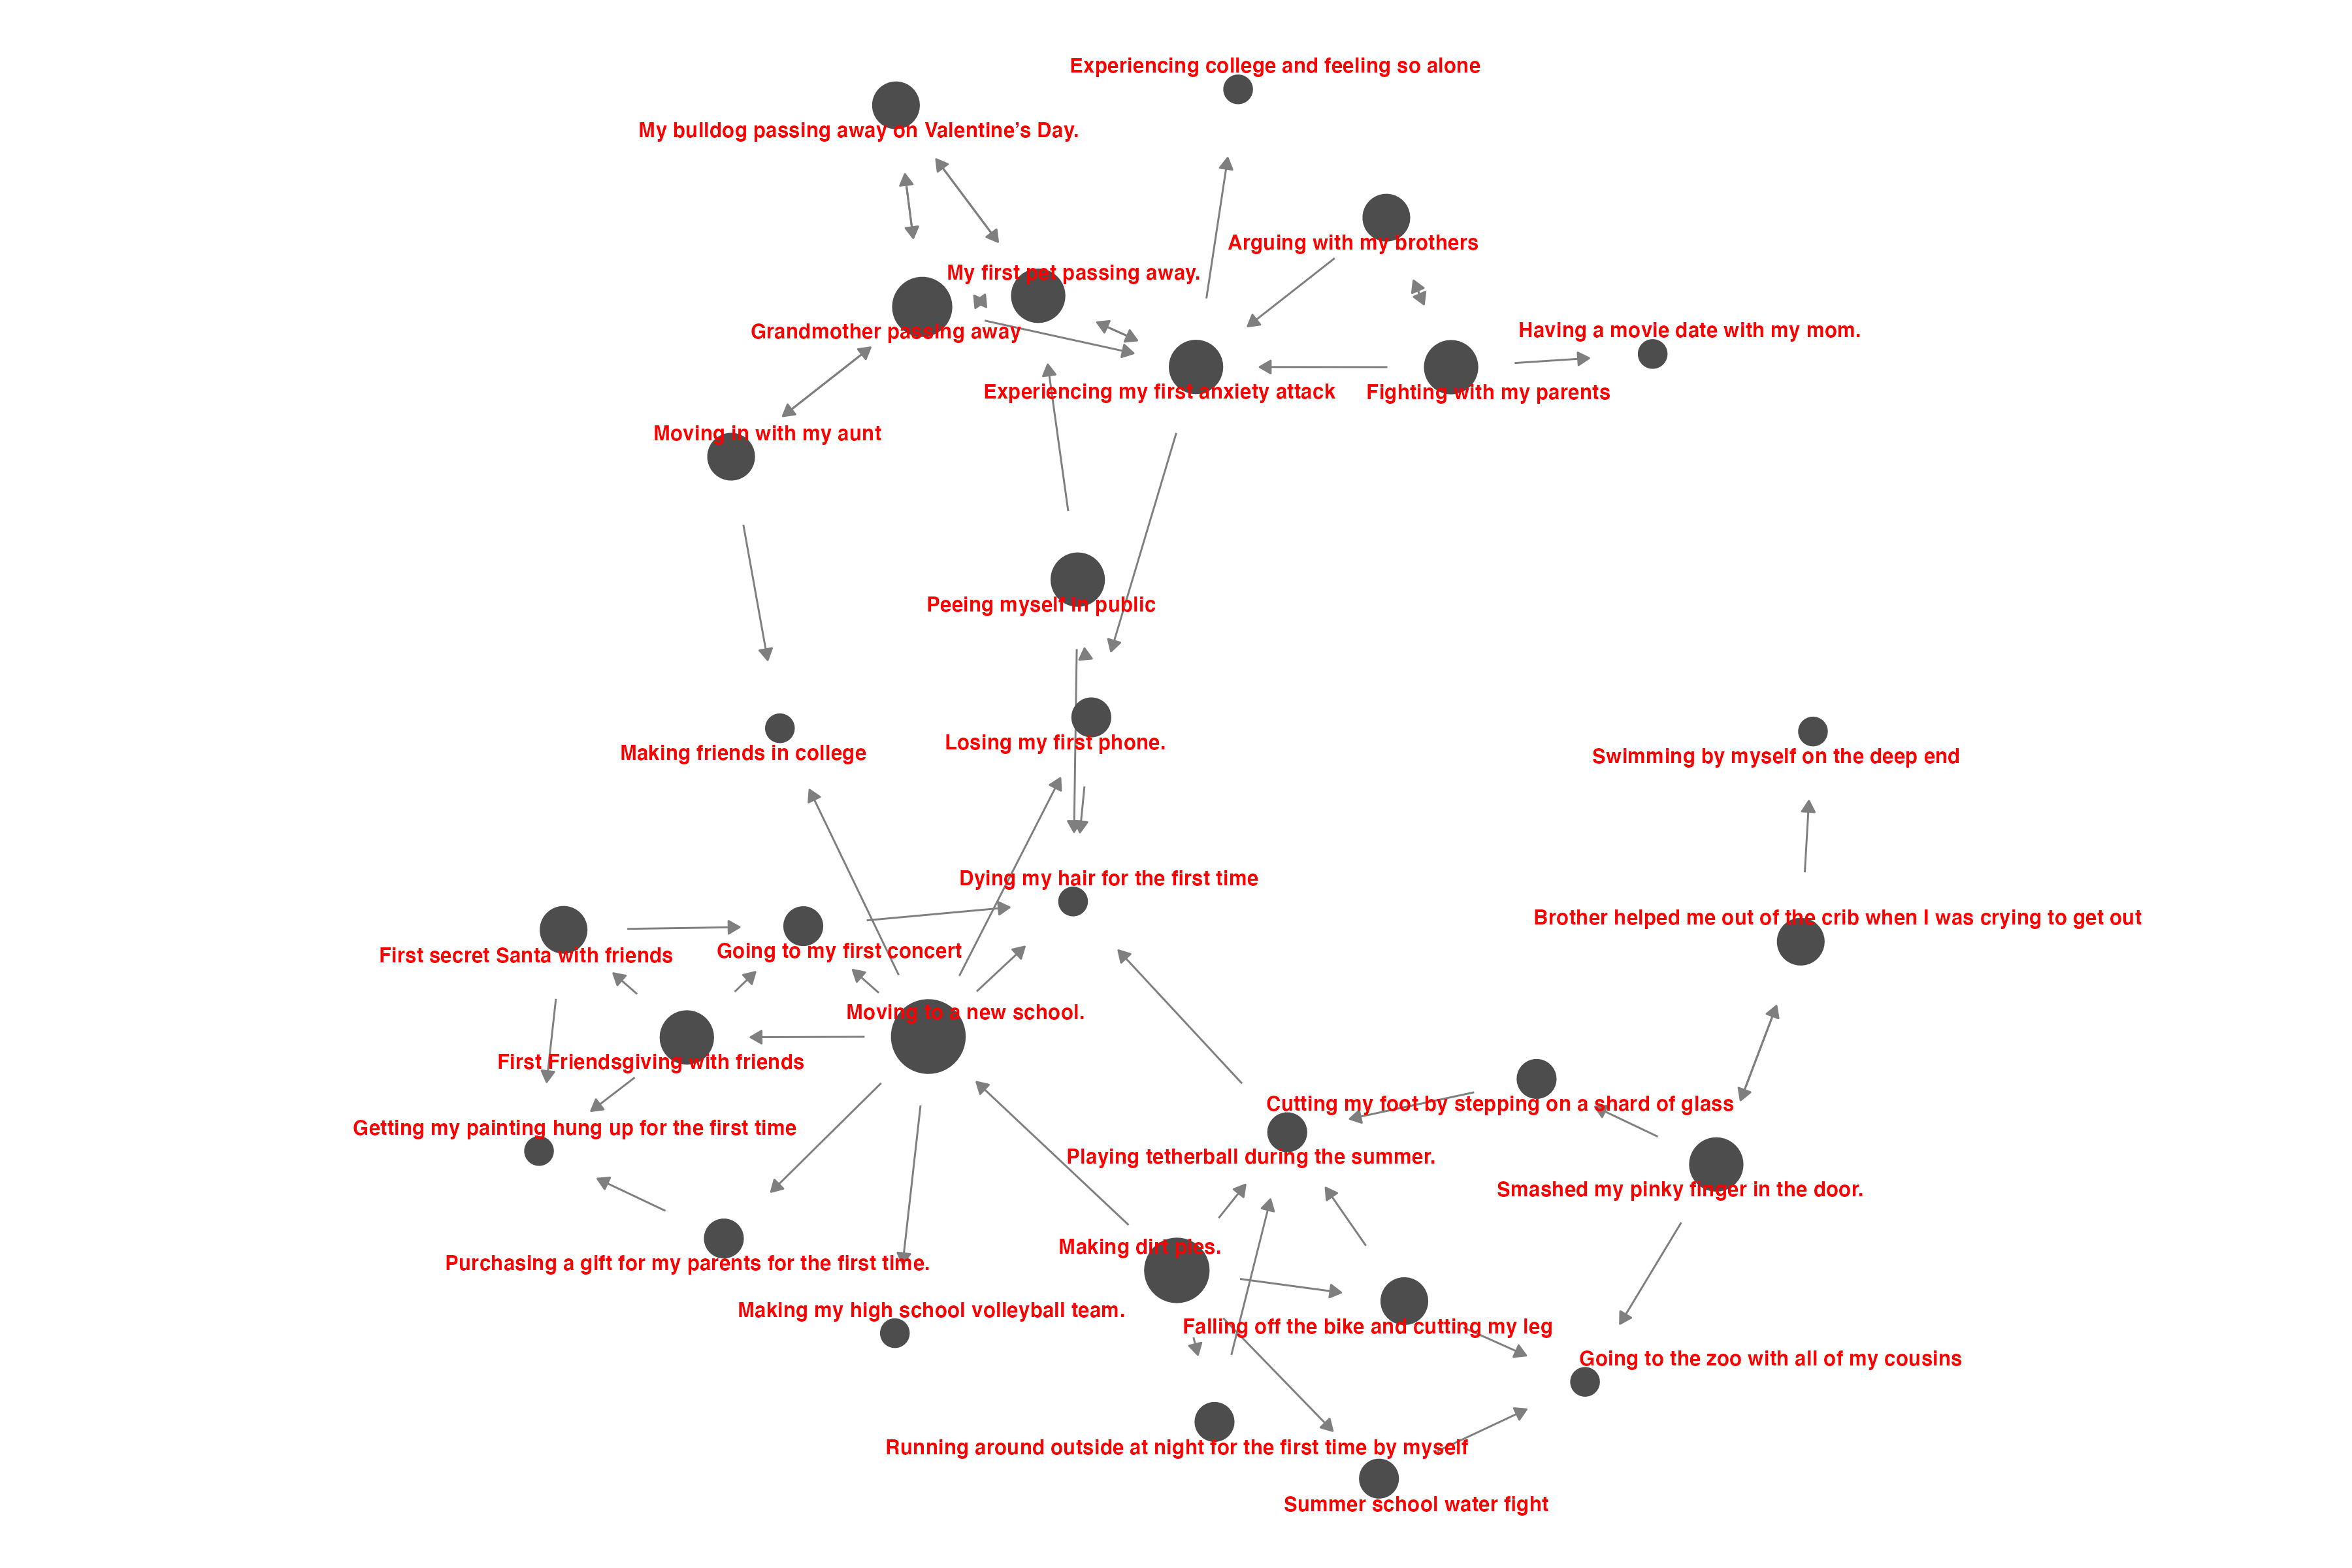
\includegraphics{images/60260_net.png}

\begin{center}\rule{0.5\linewidth}{0.5pt}\end{center}

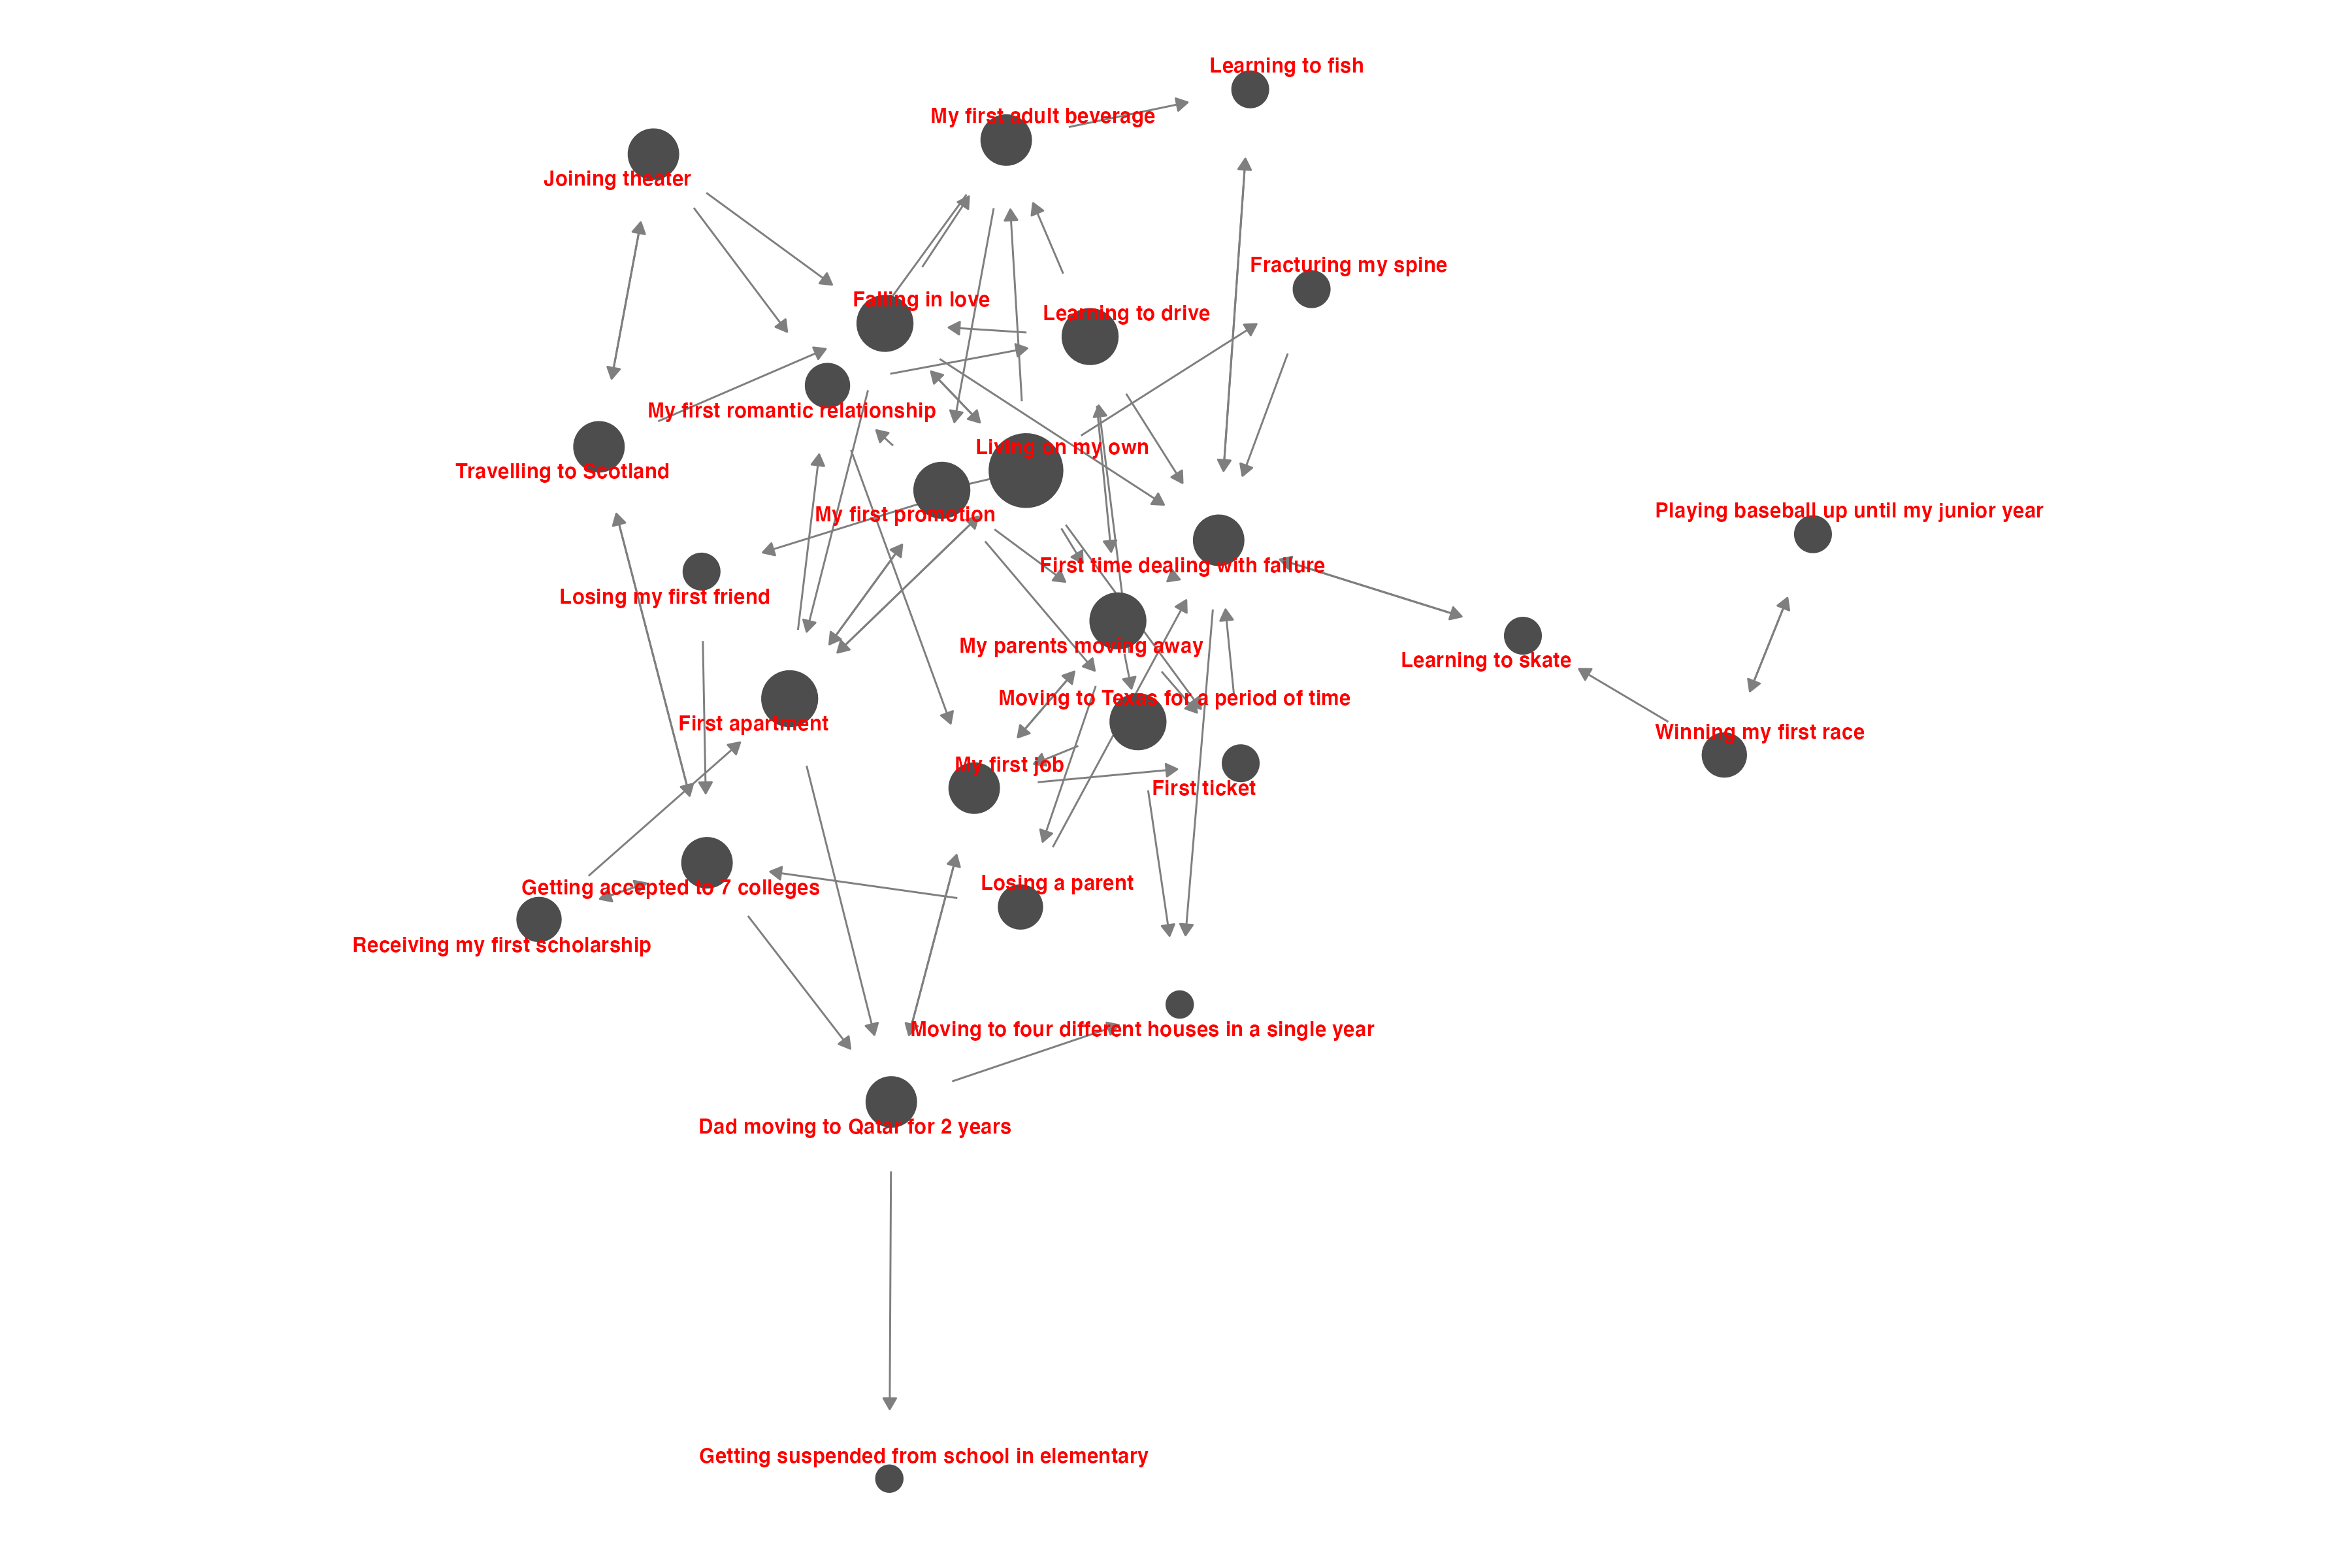
\includegraphics{images/60571_net.png}

\begin{center}\rule{0.5\linewidth}{0.5pt}\end{center}

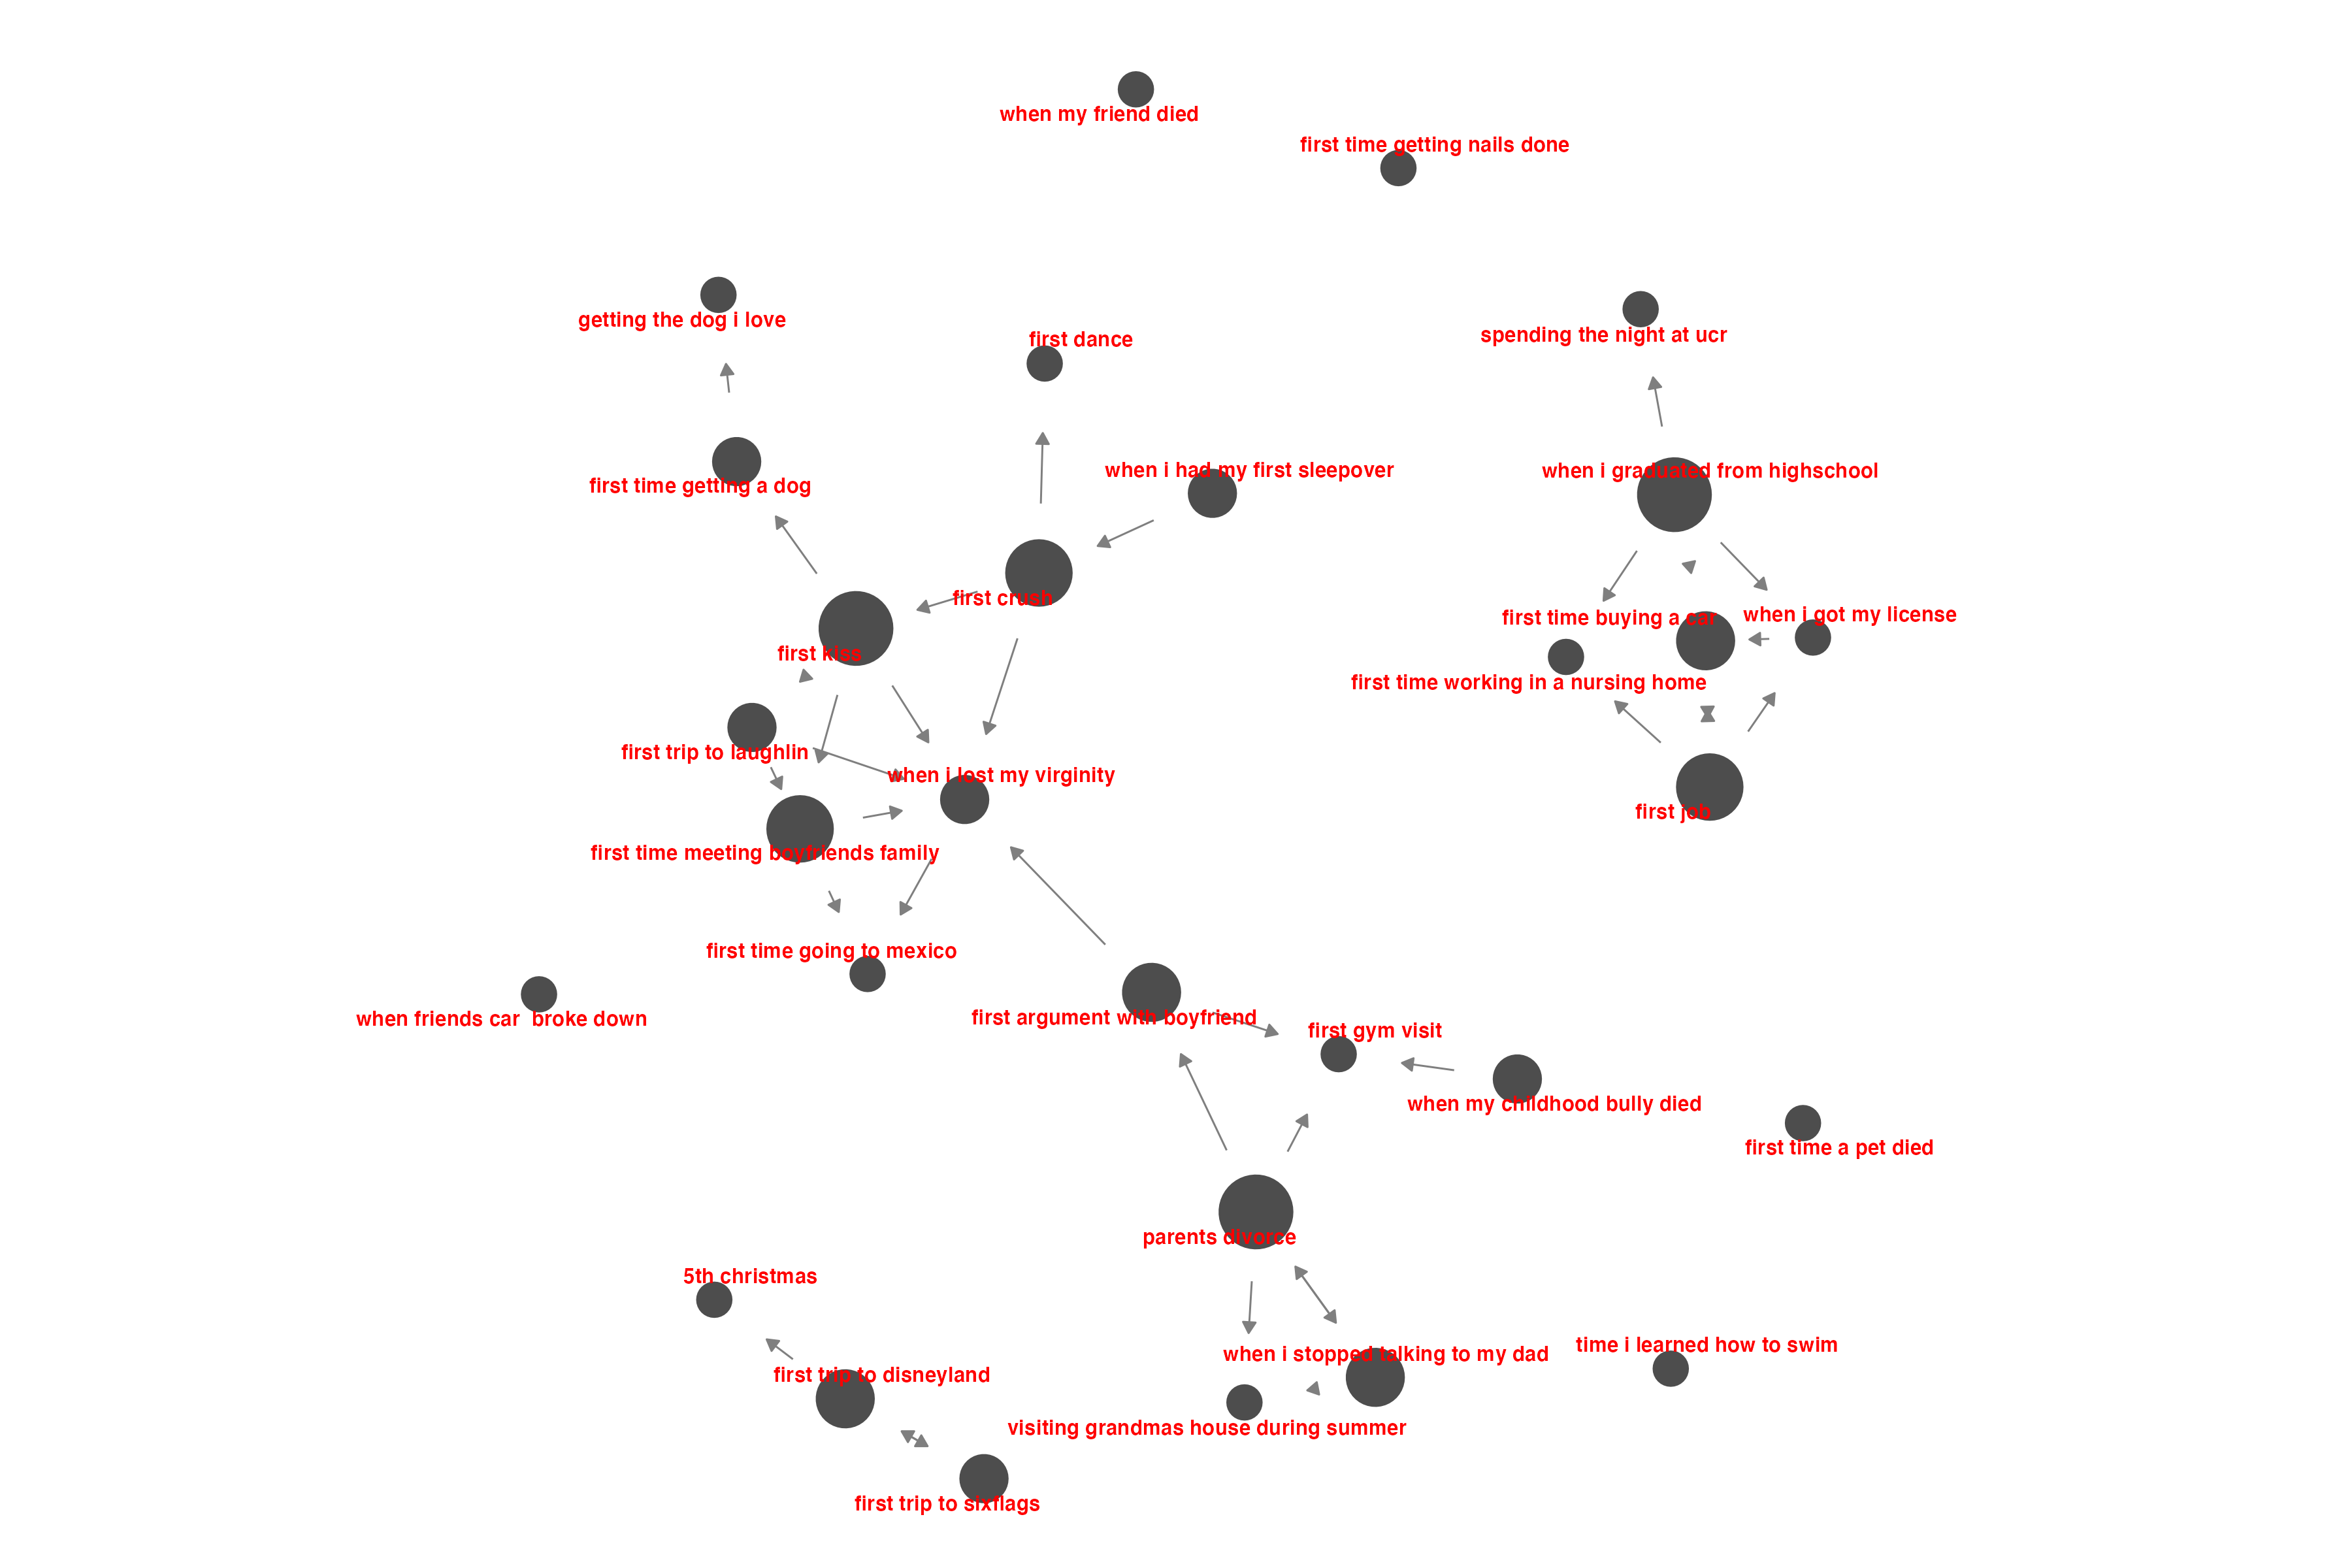
\includegraphics{images/60572_net.png}

\begin{center}\rule{0.5\linewidth}{0.5pt}\end{center}

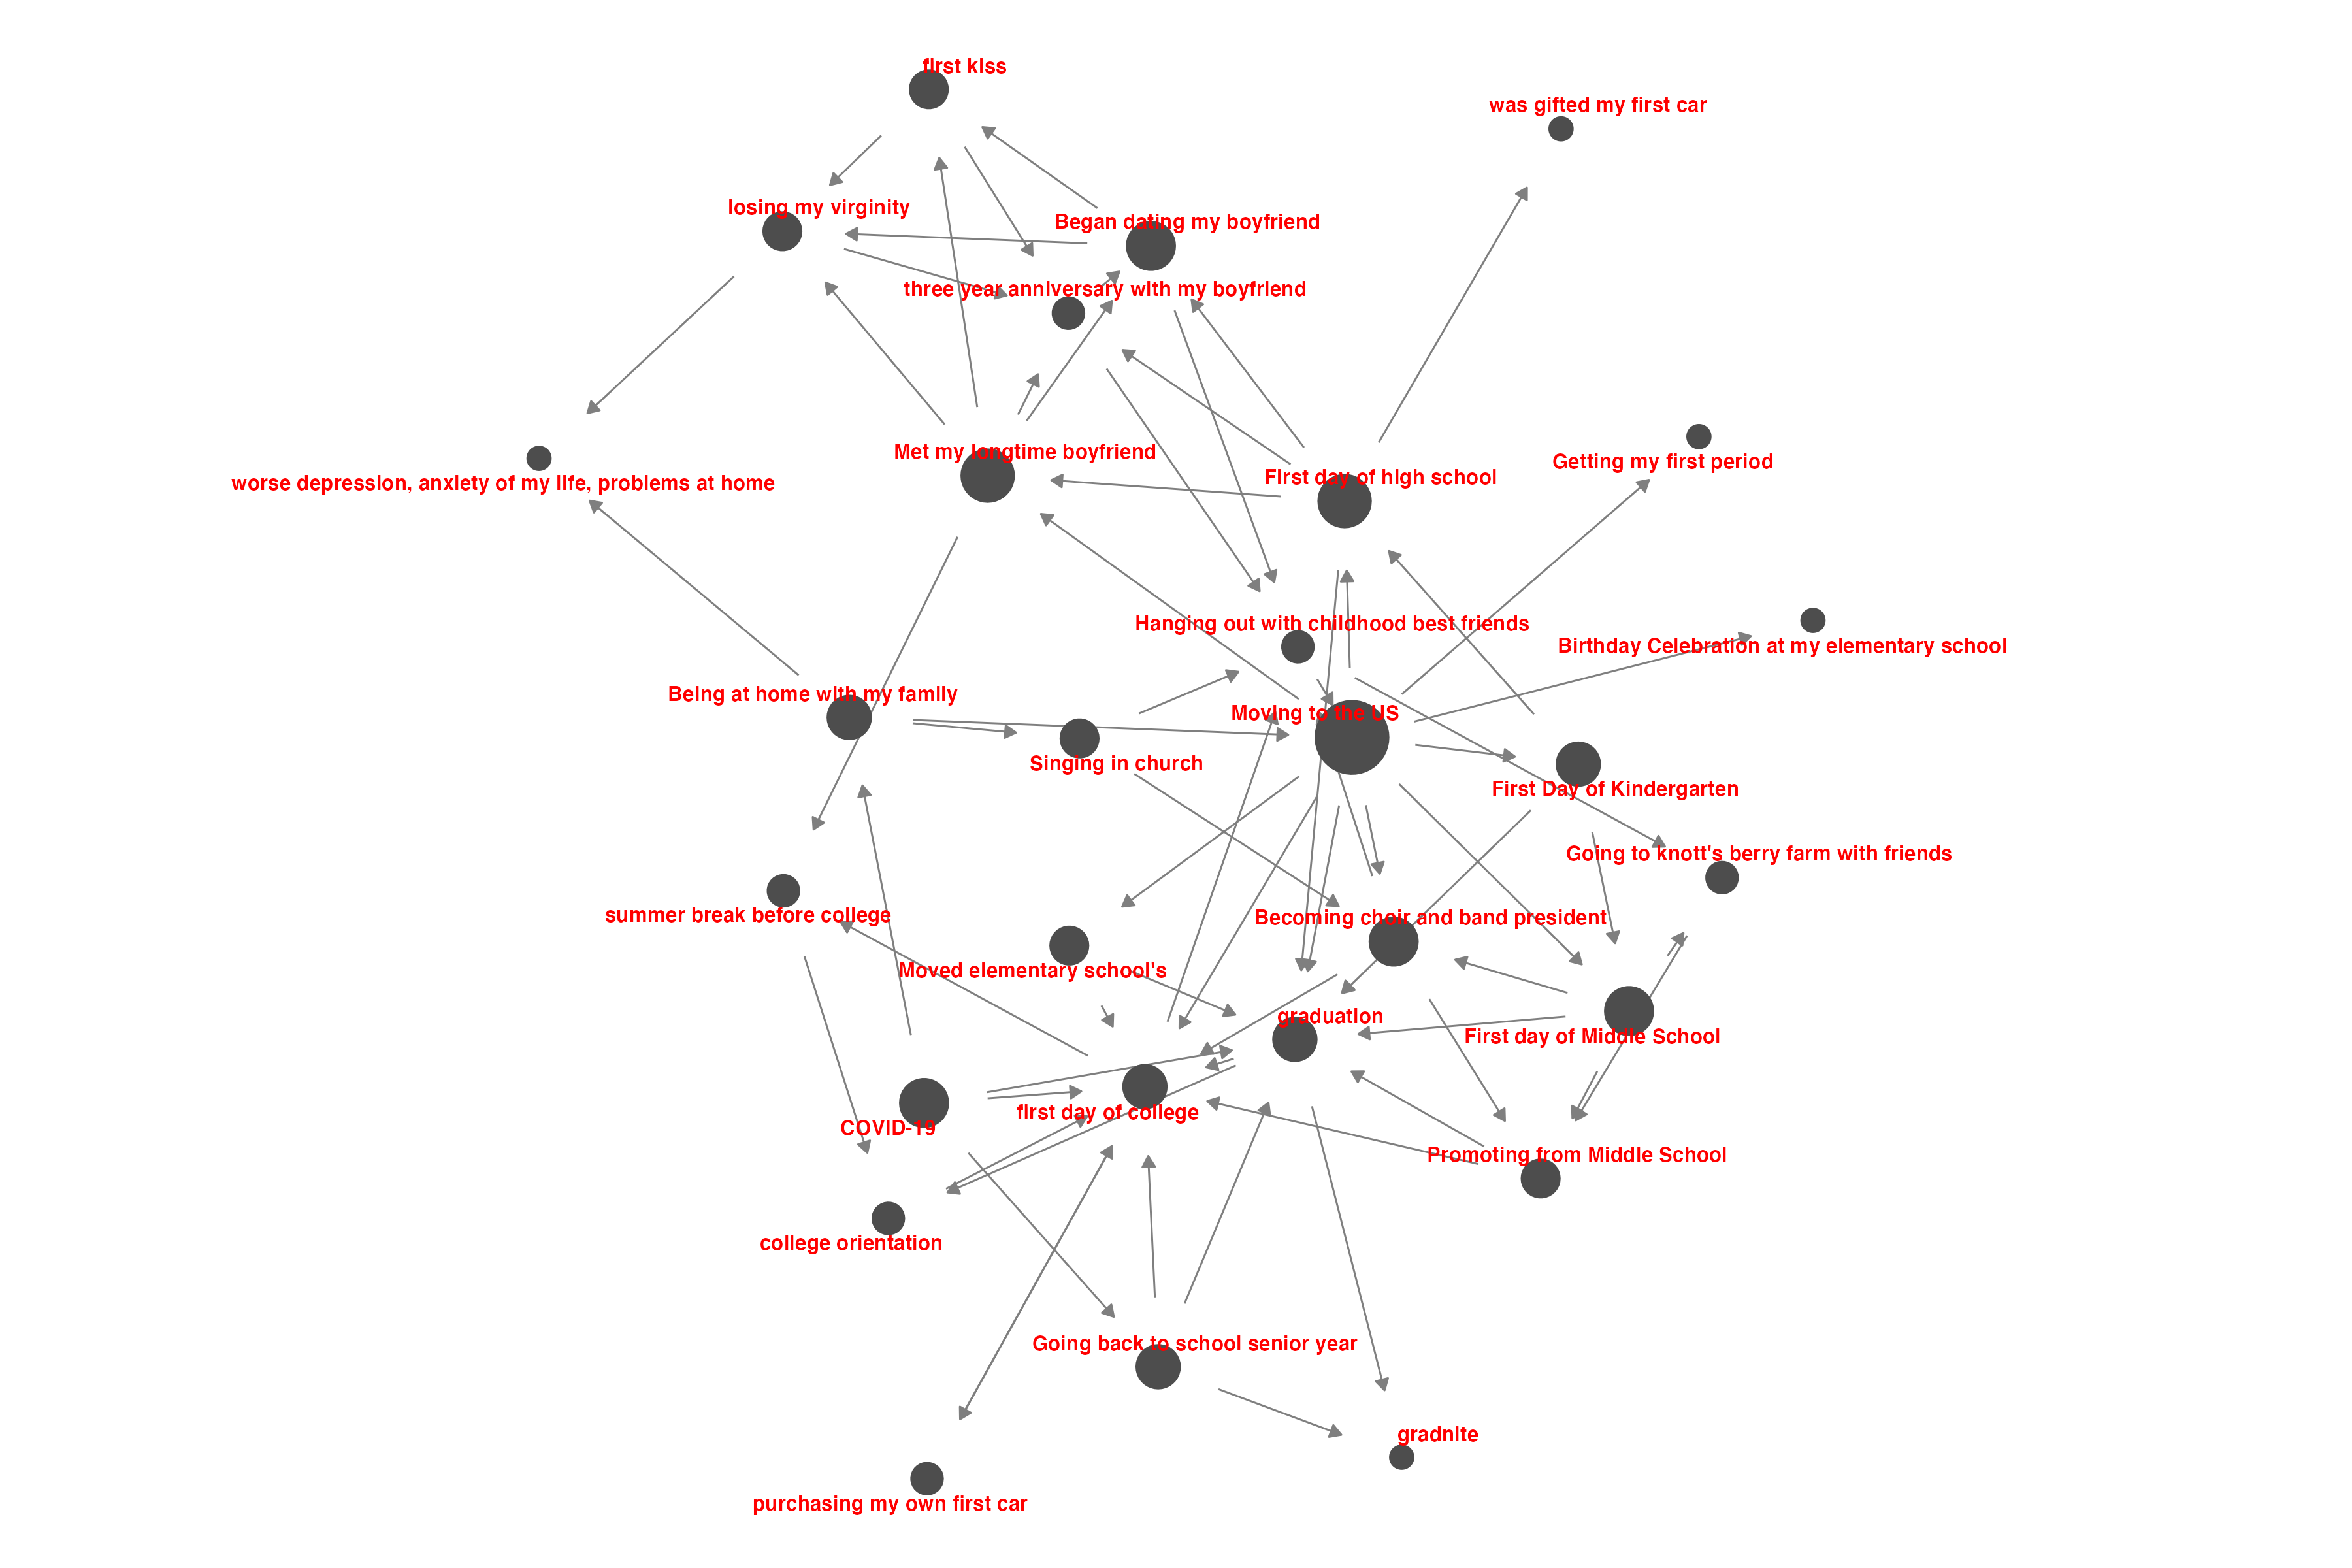
\includegraphics{images/60928_net.png}

\begin{center}\rule{0.5\linewidth}{0.5pt}\end{center}

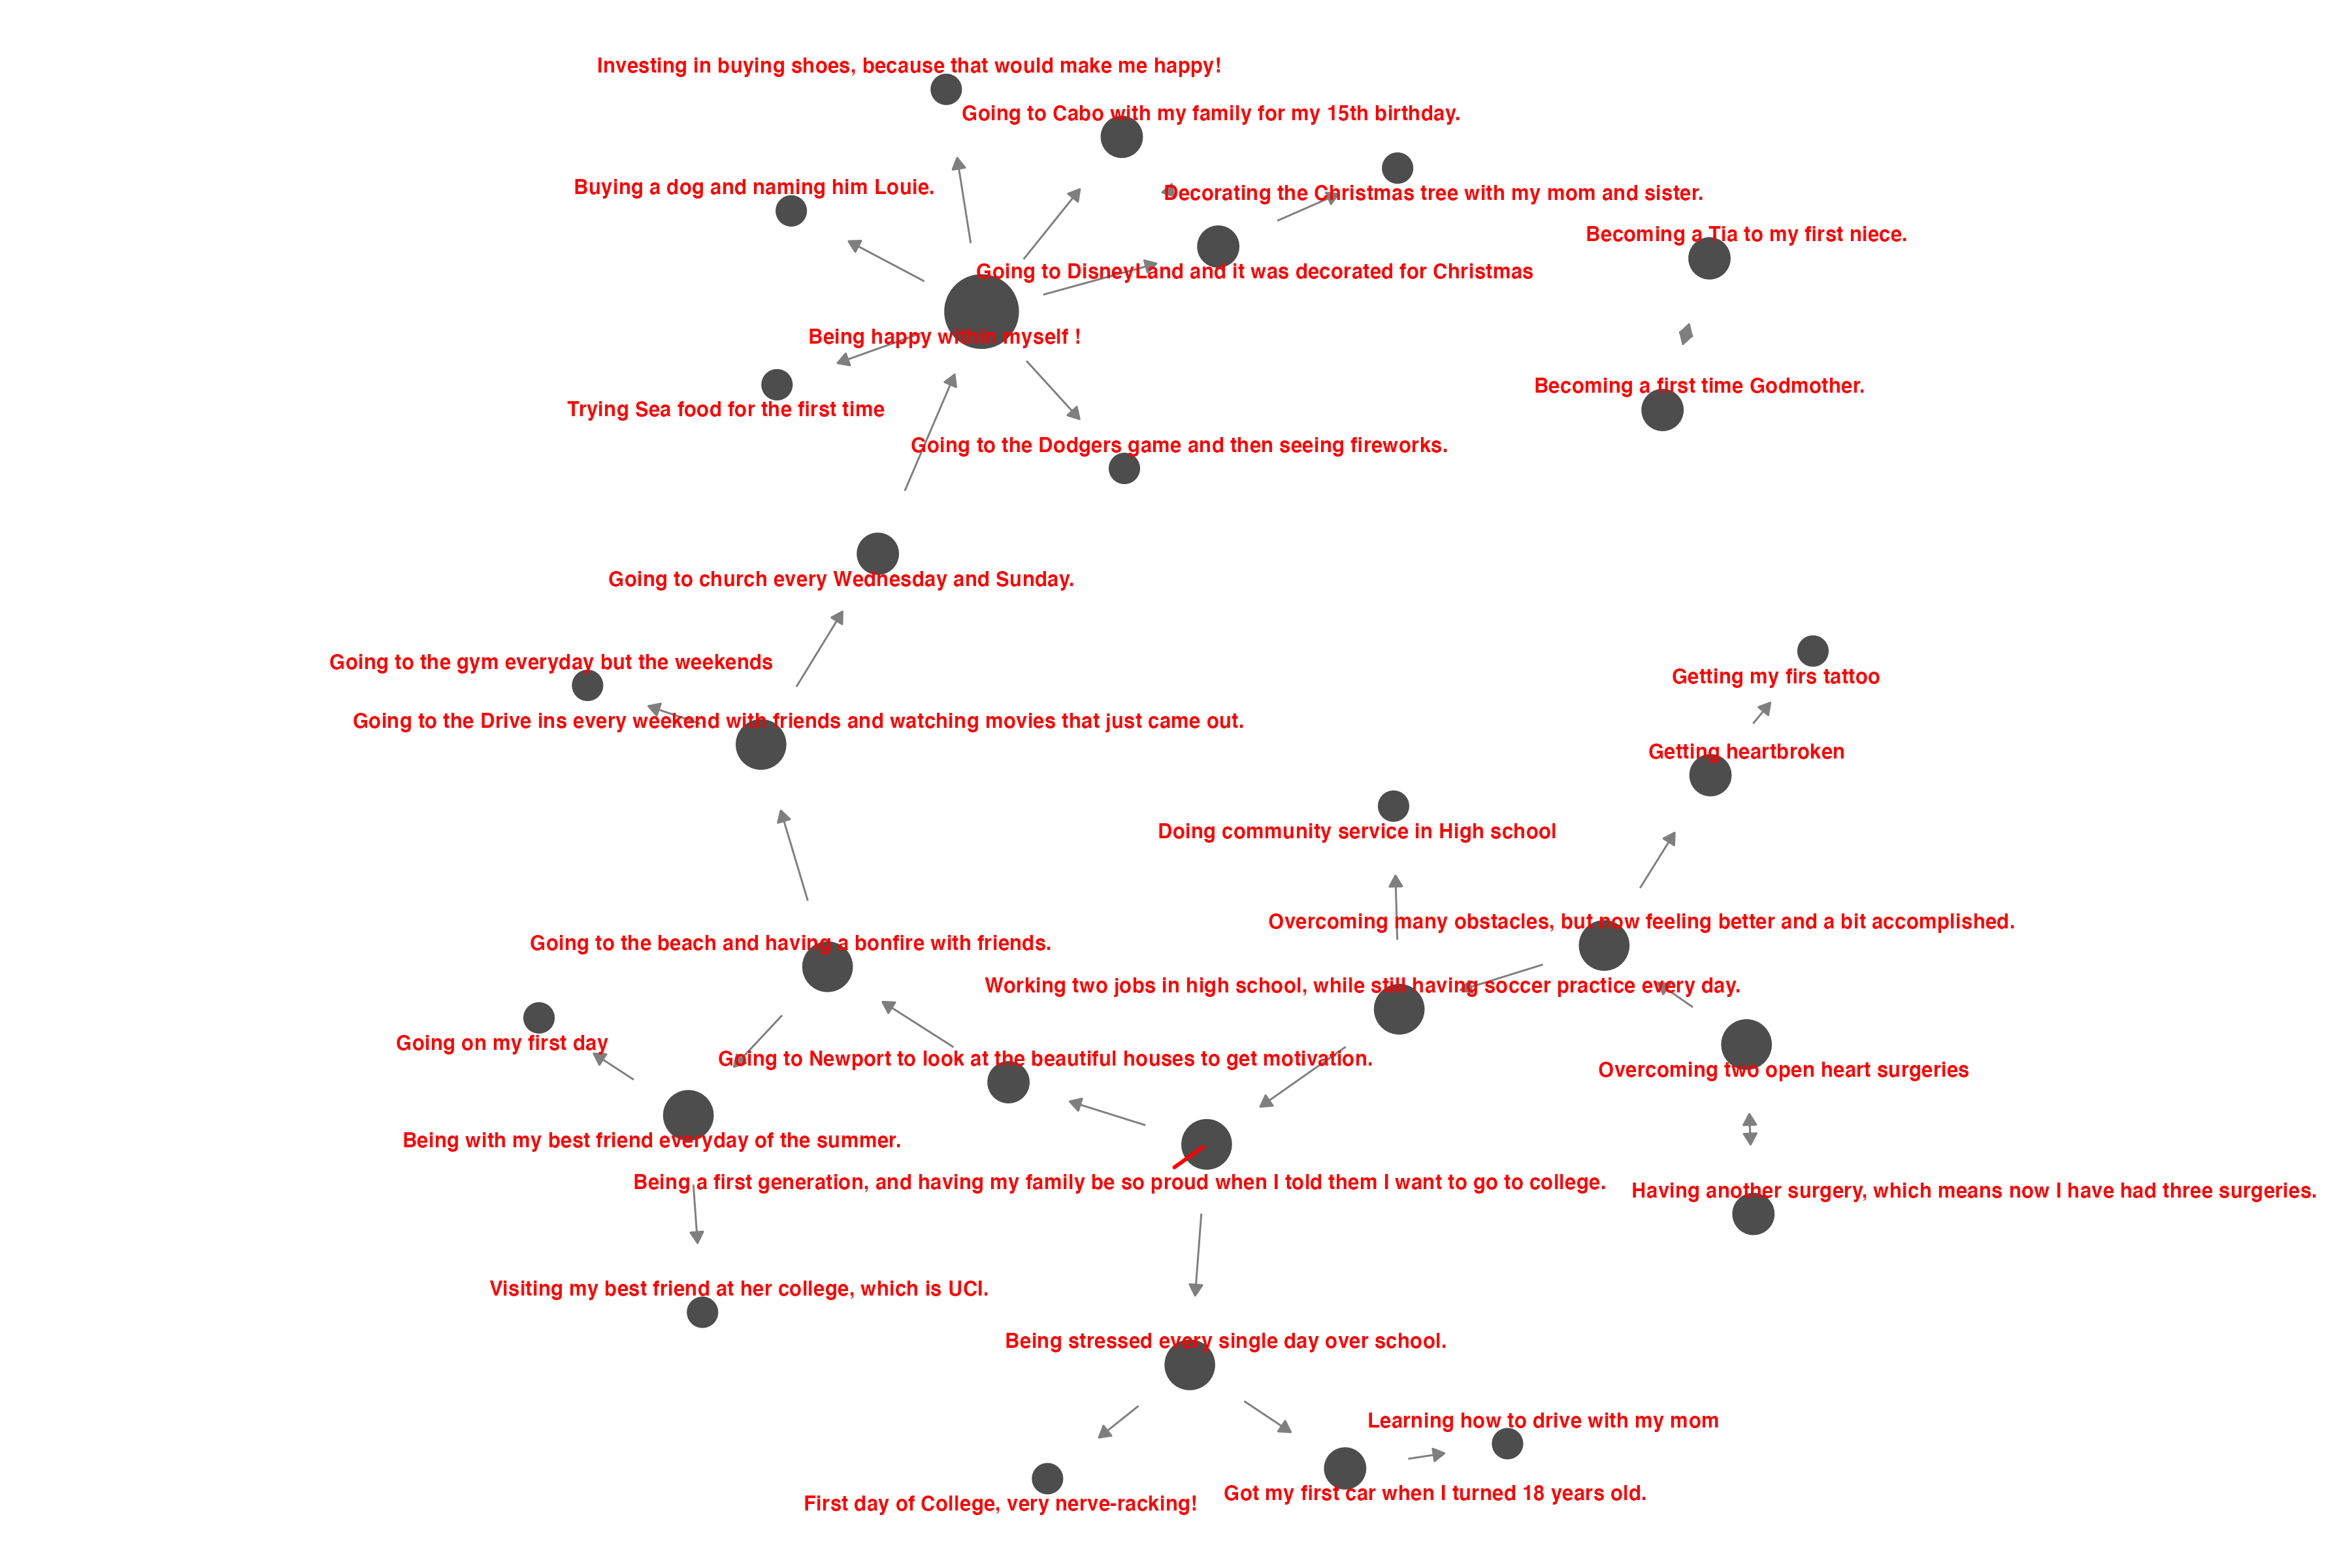
\includegraphics{images/60950_net.png}

\begin{center}\rule{0.5\linewidth}{0.5pt}\end{center}

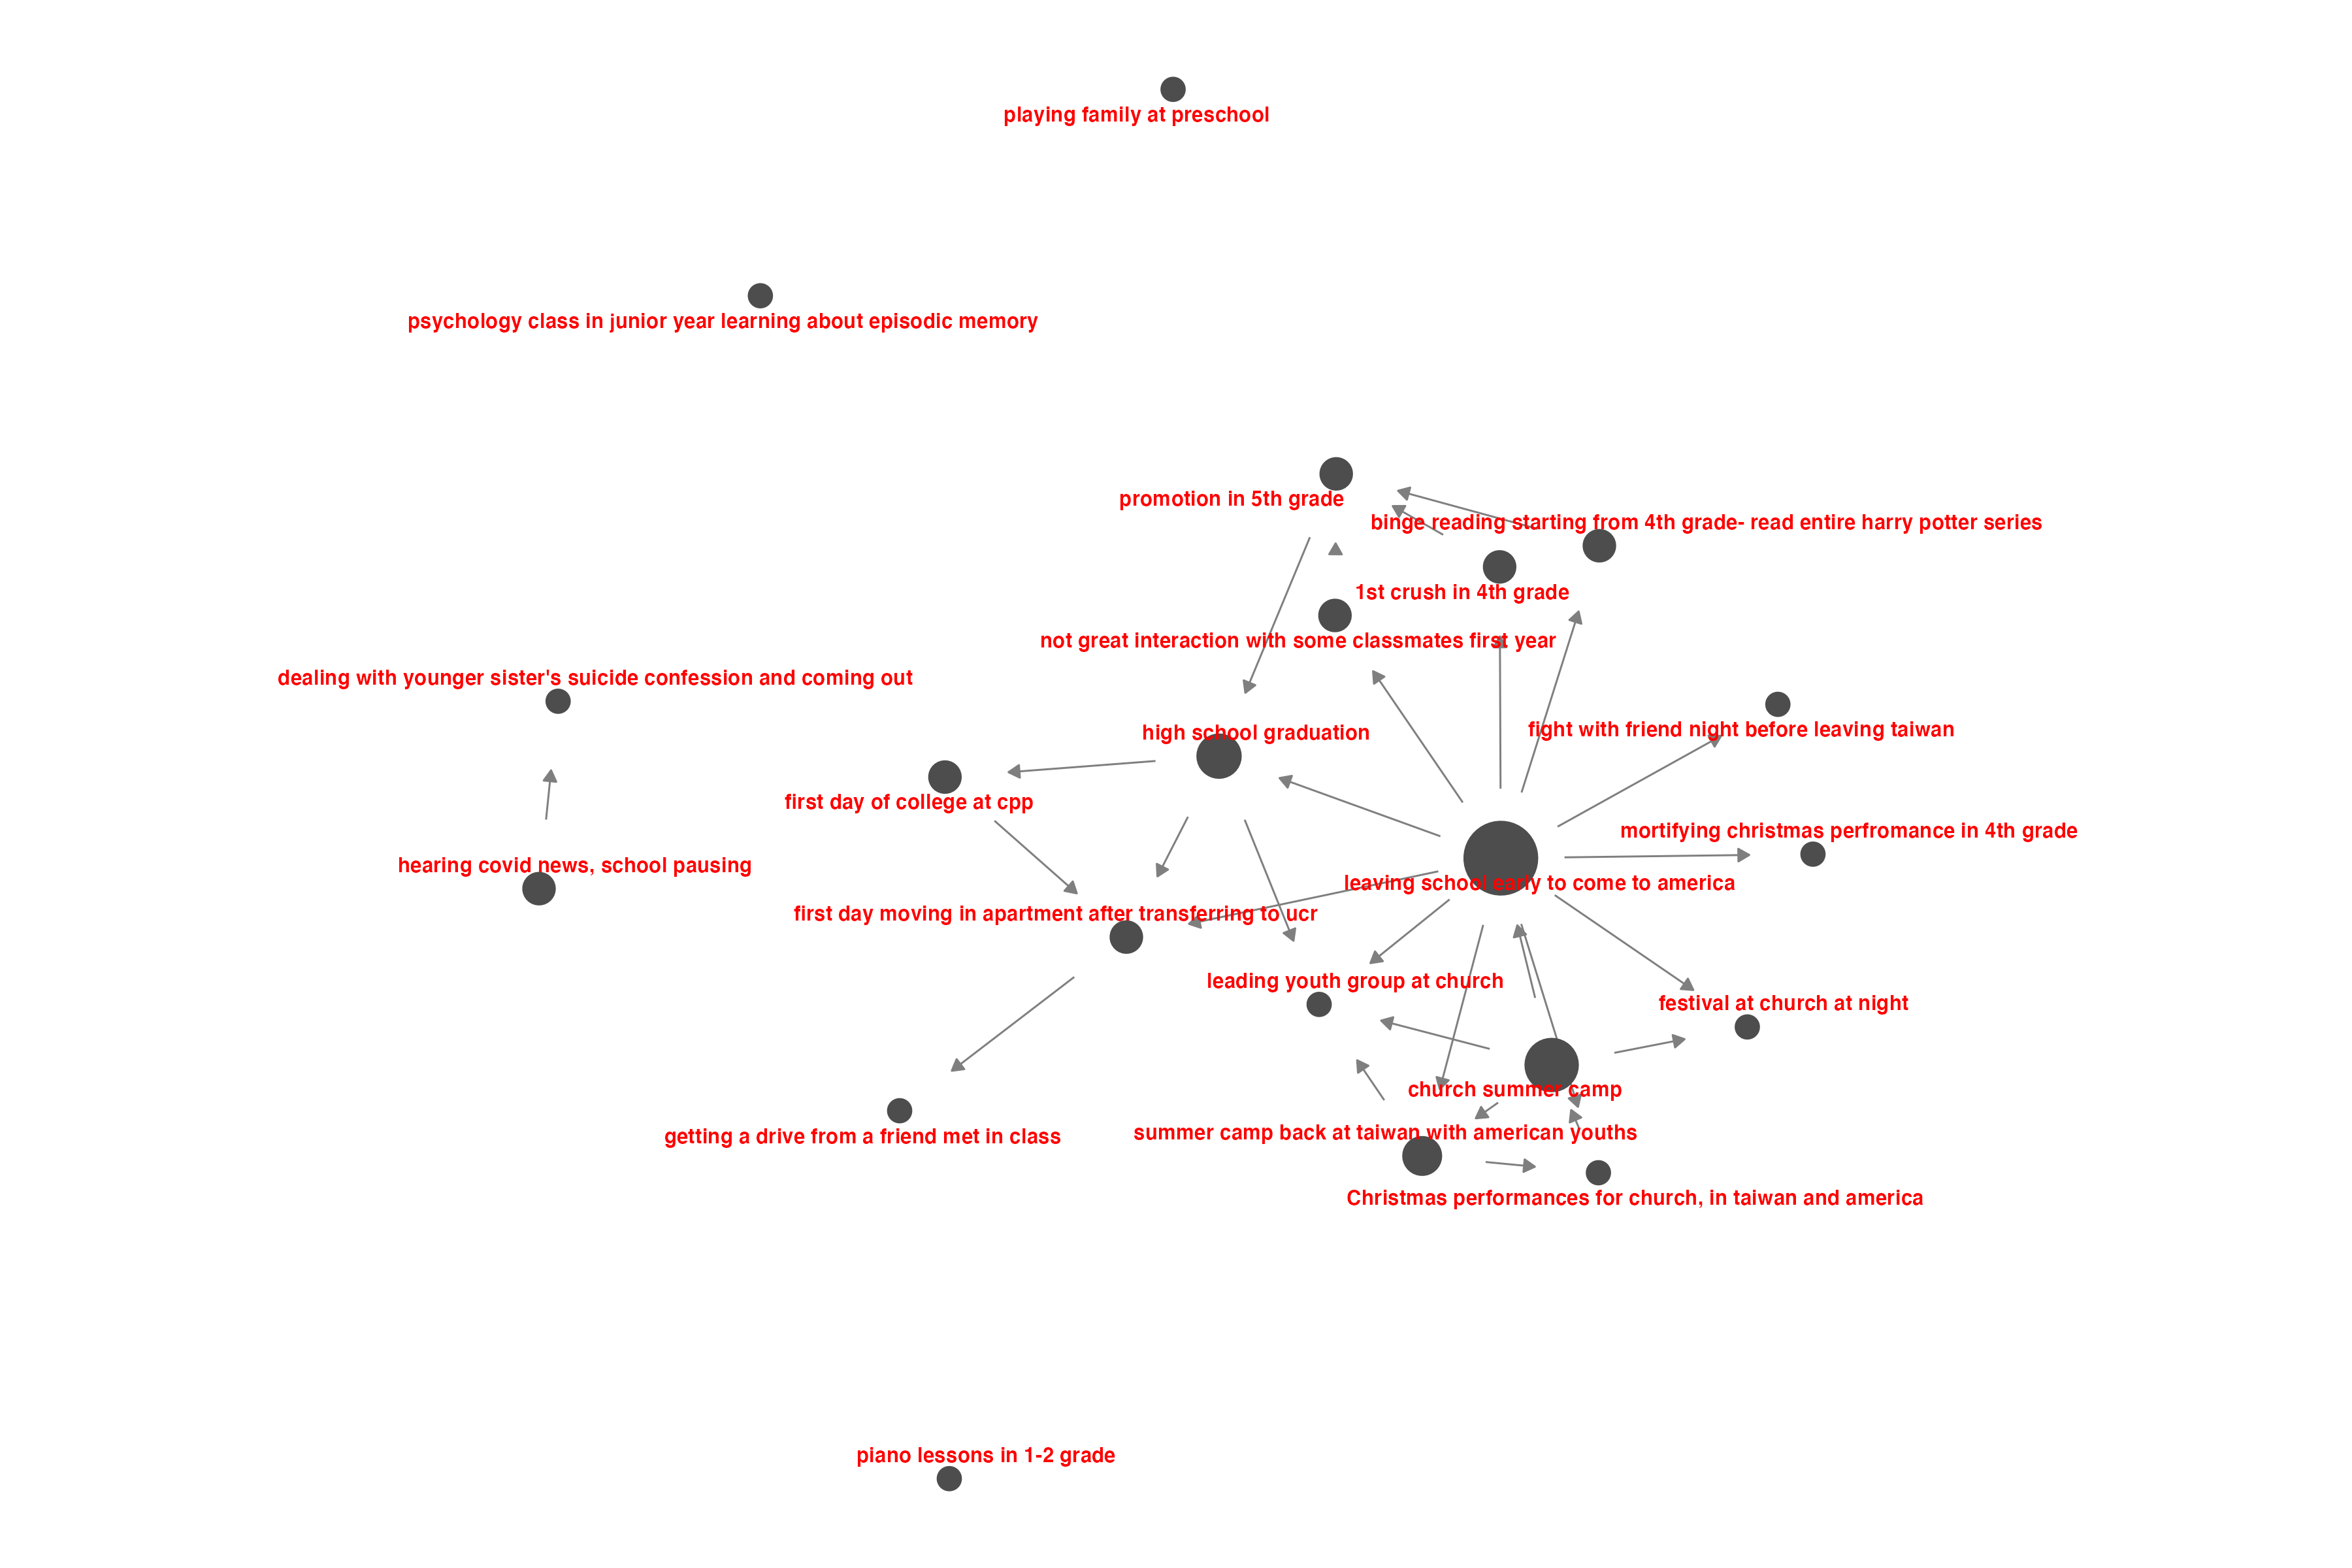
\includegraphics{images/61024_net.png}

\begin{center}\rule{0.5\linewidth}{0.5pt}\end{center}

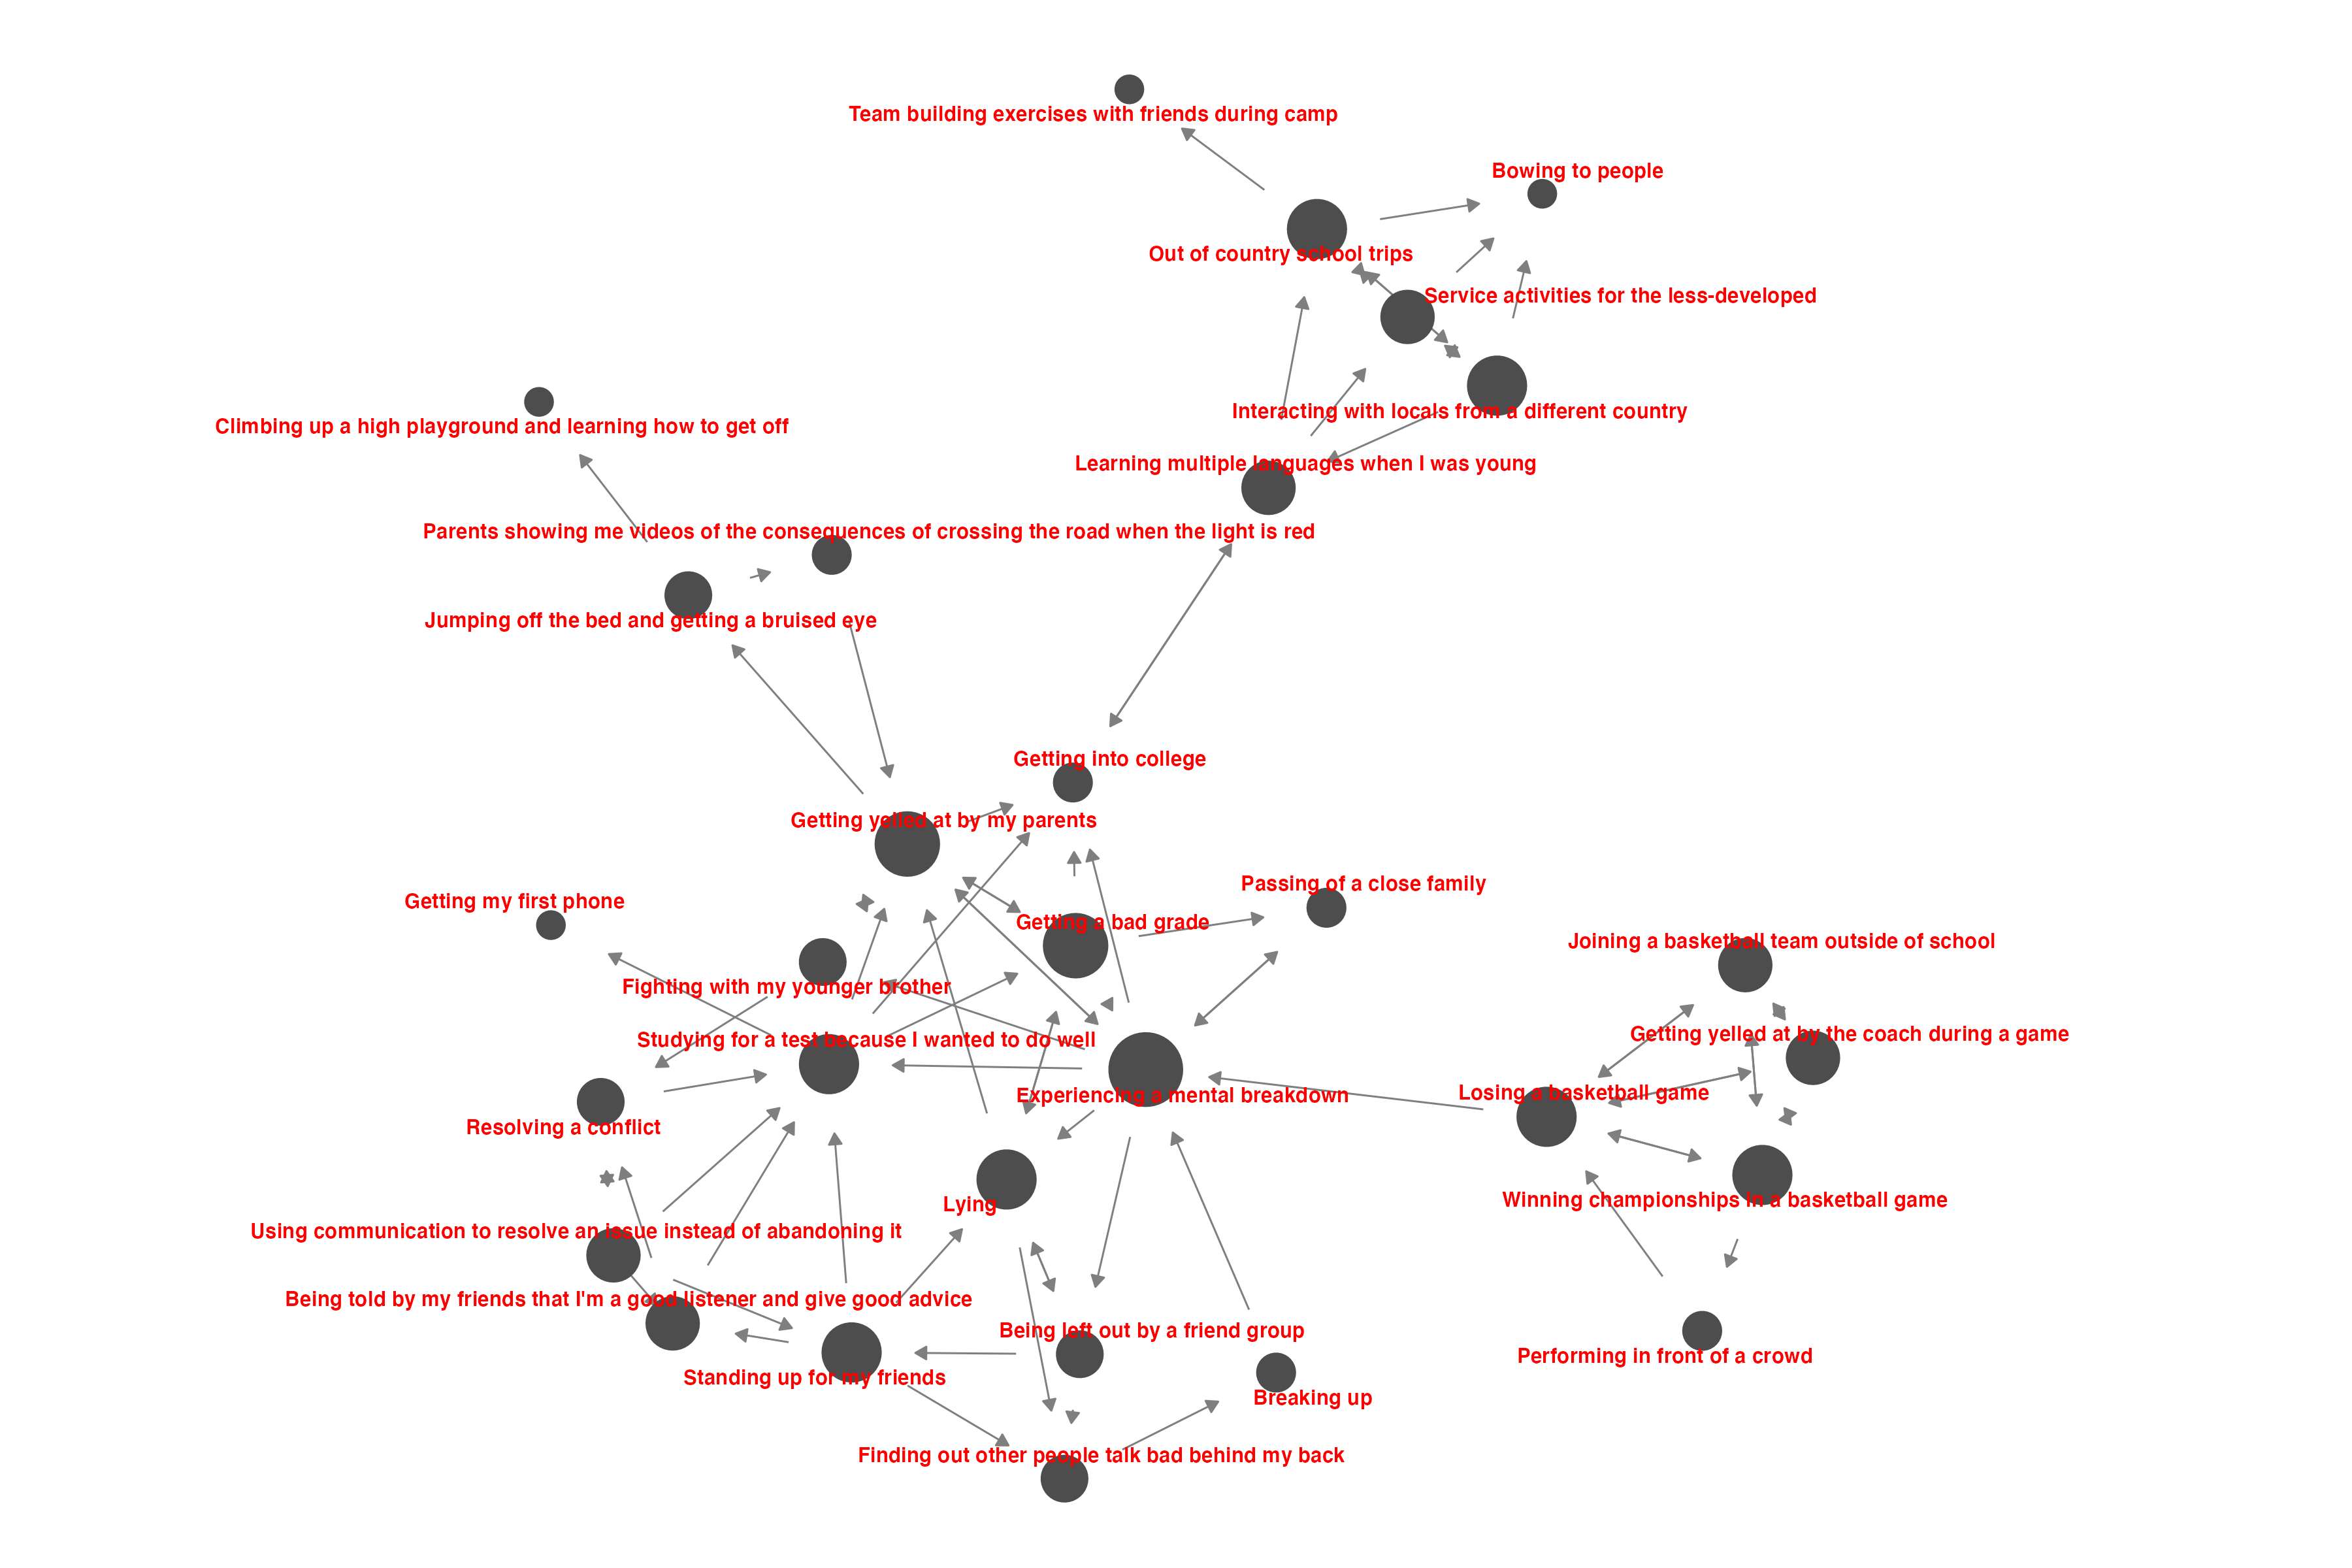
\includegraphics{images/61059_net.png}

\begin{center}\rule{0.5\linewidth}{0.5pt}\end{center}

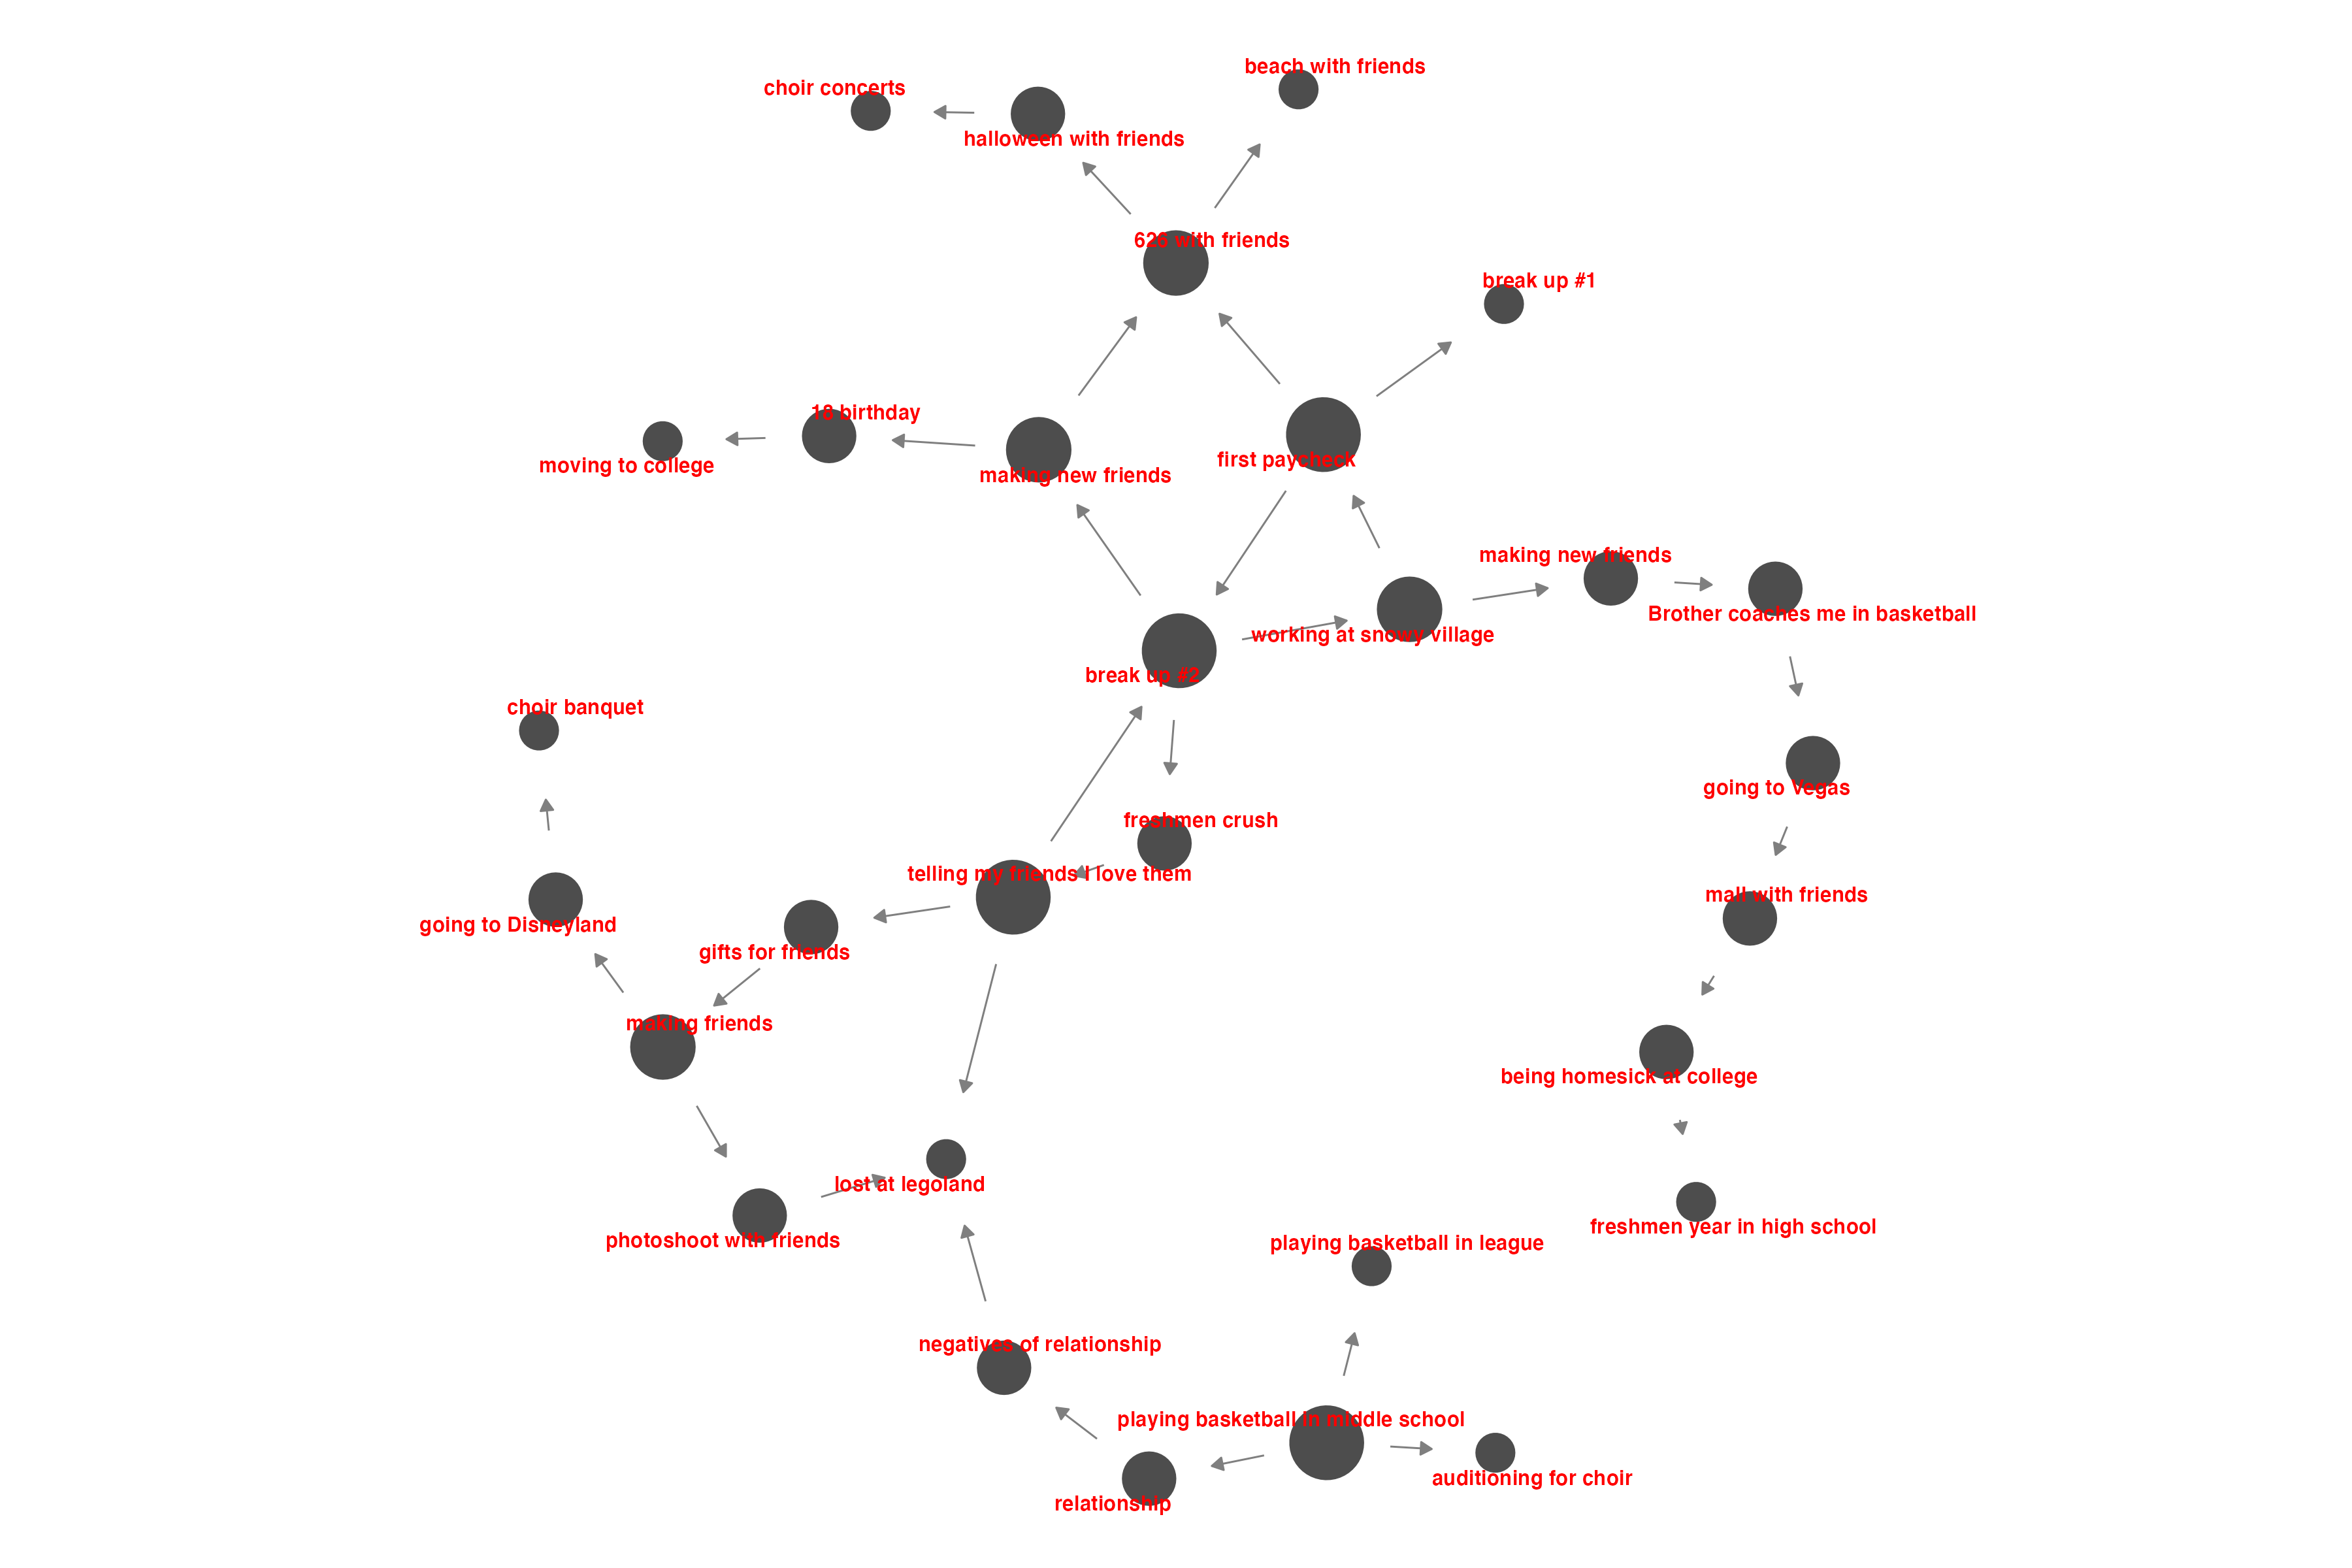
\includegraphics{images/62097_net.png}

\begin{center}\rule{0.5\linewidth}{0.5pt}\end{center}

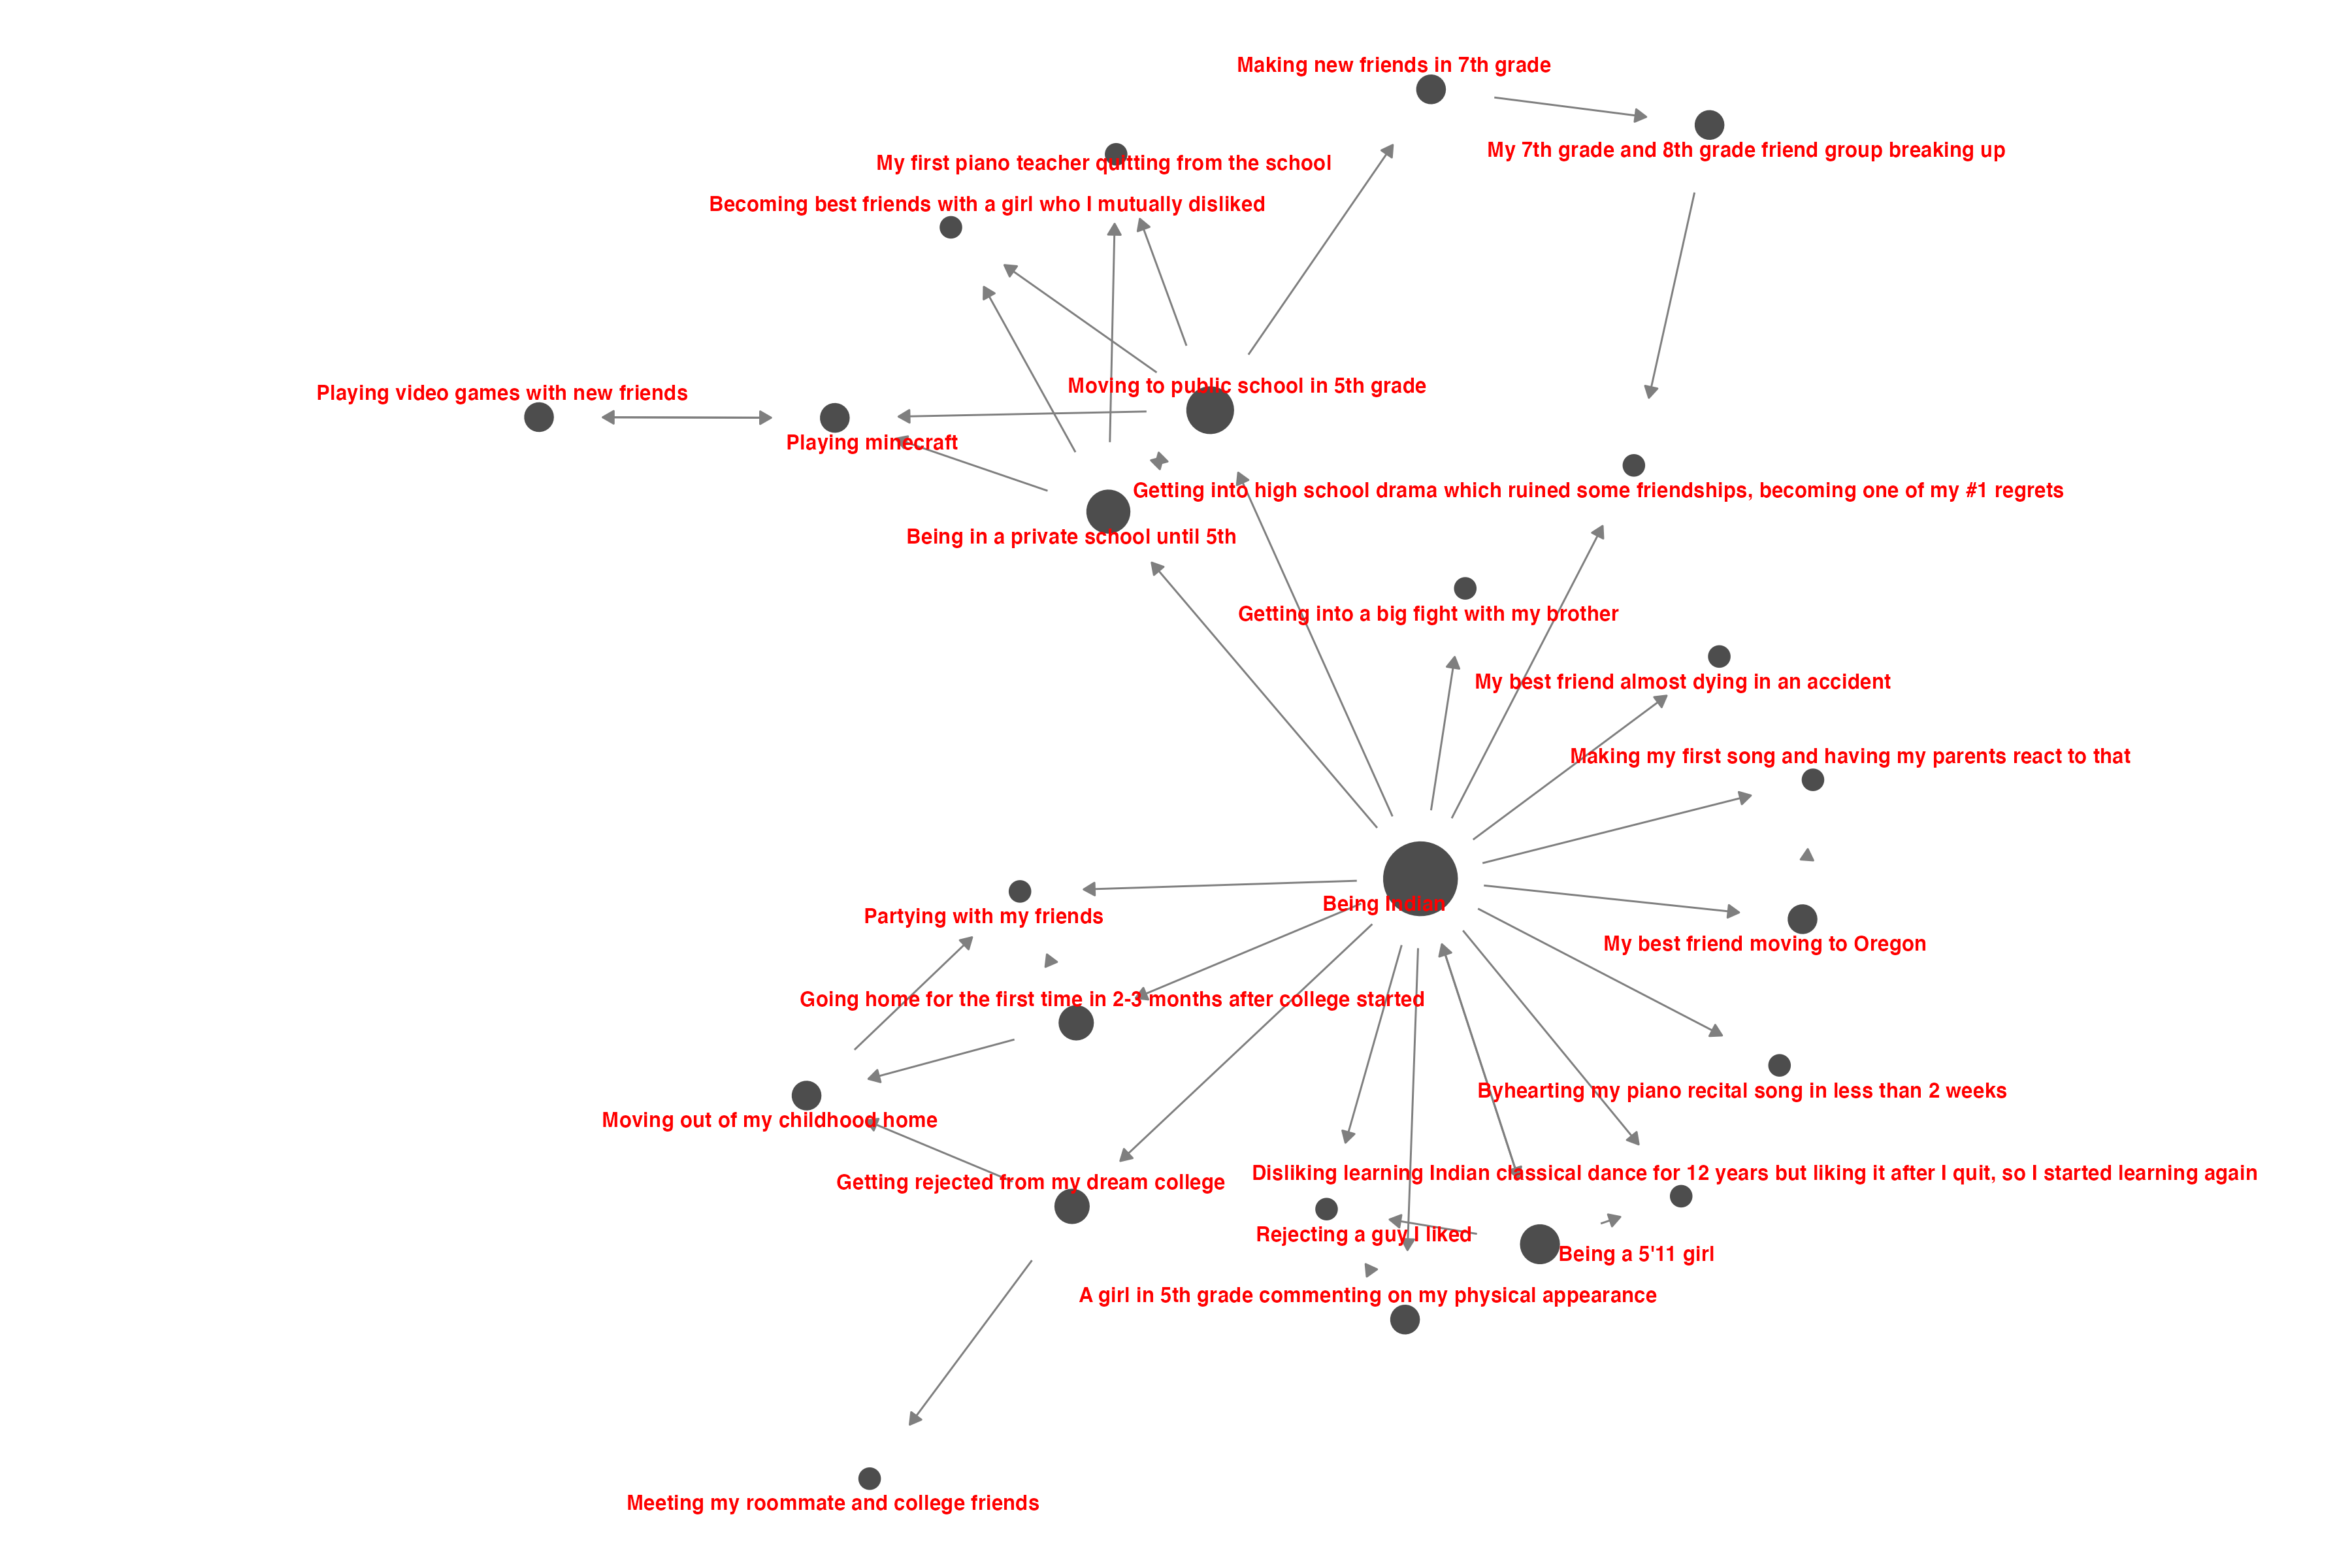
\includegraphics{images/62002_net.png}

\begin{center}\rule{0.5\linewidth}{0.5pt}\end{center}

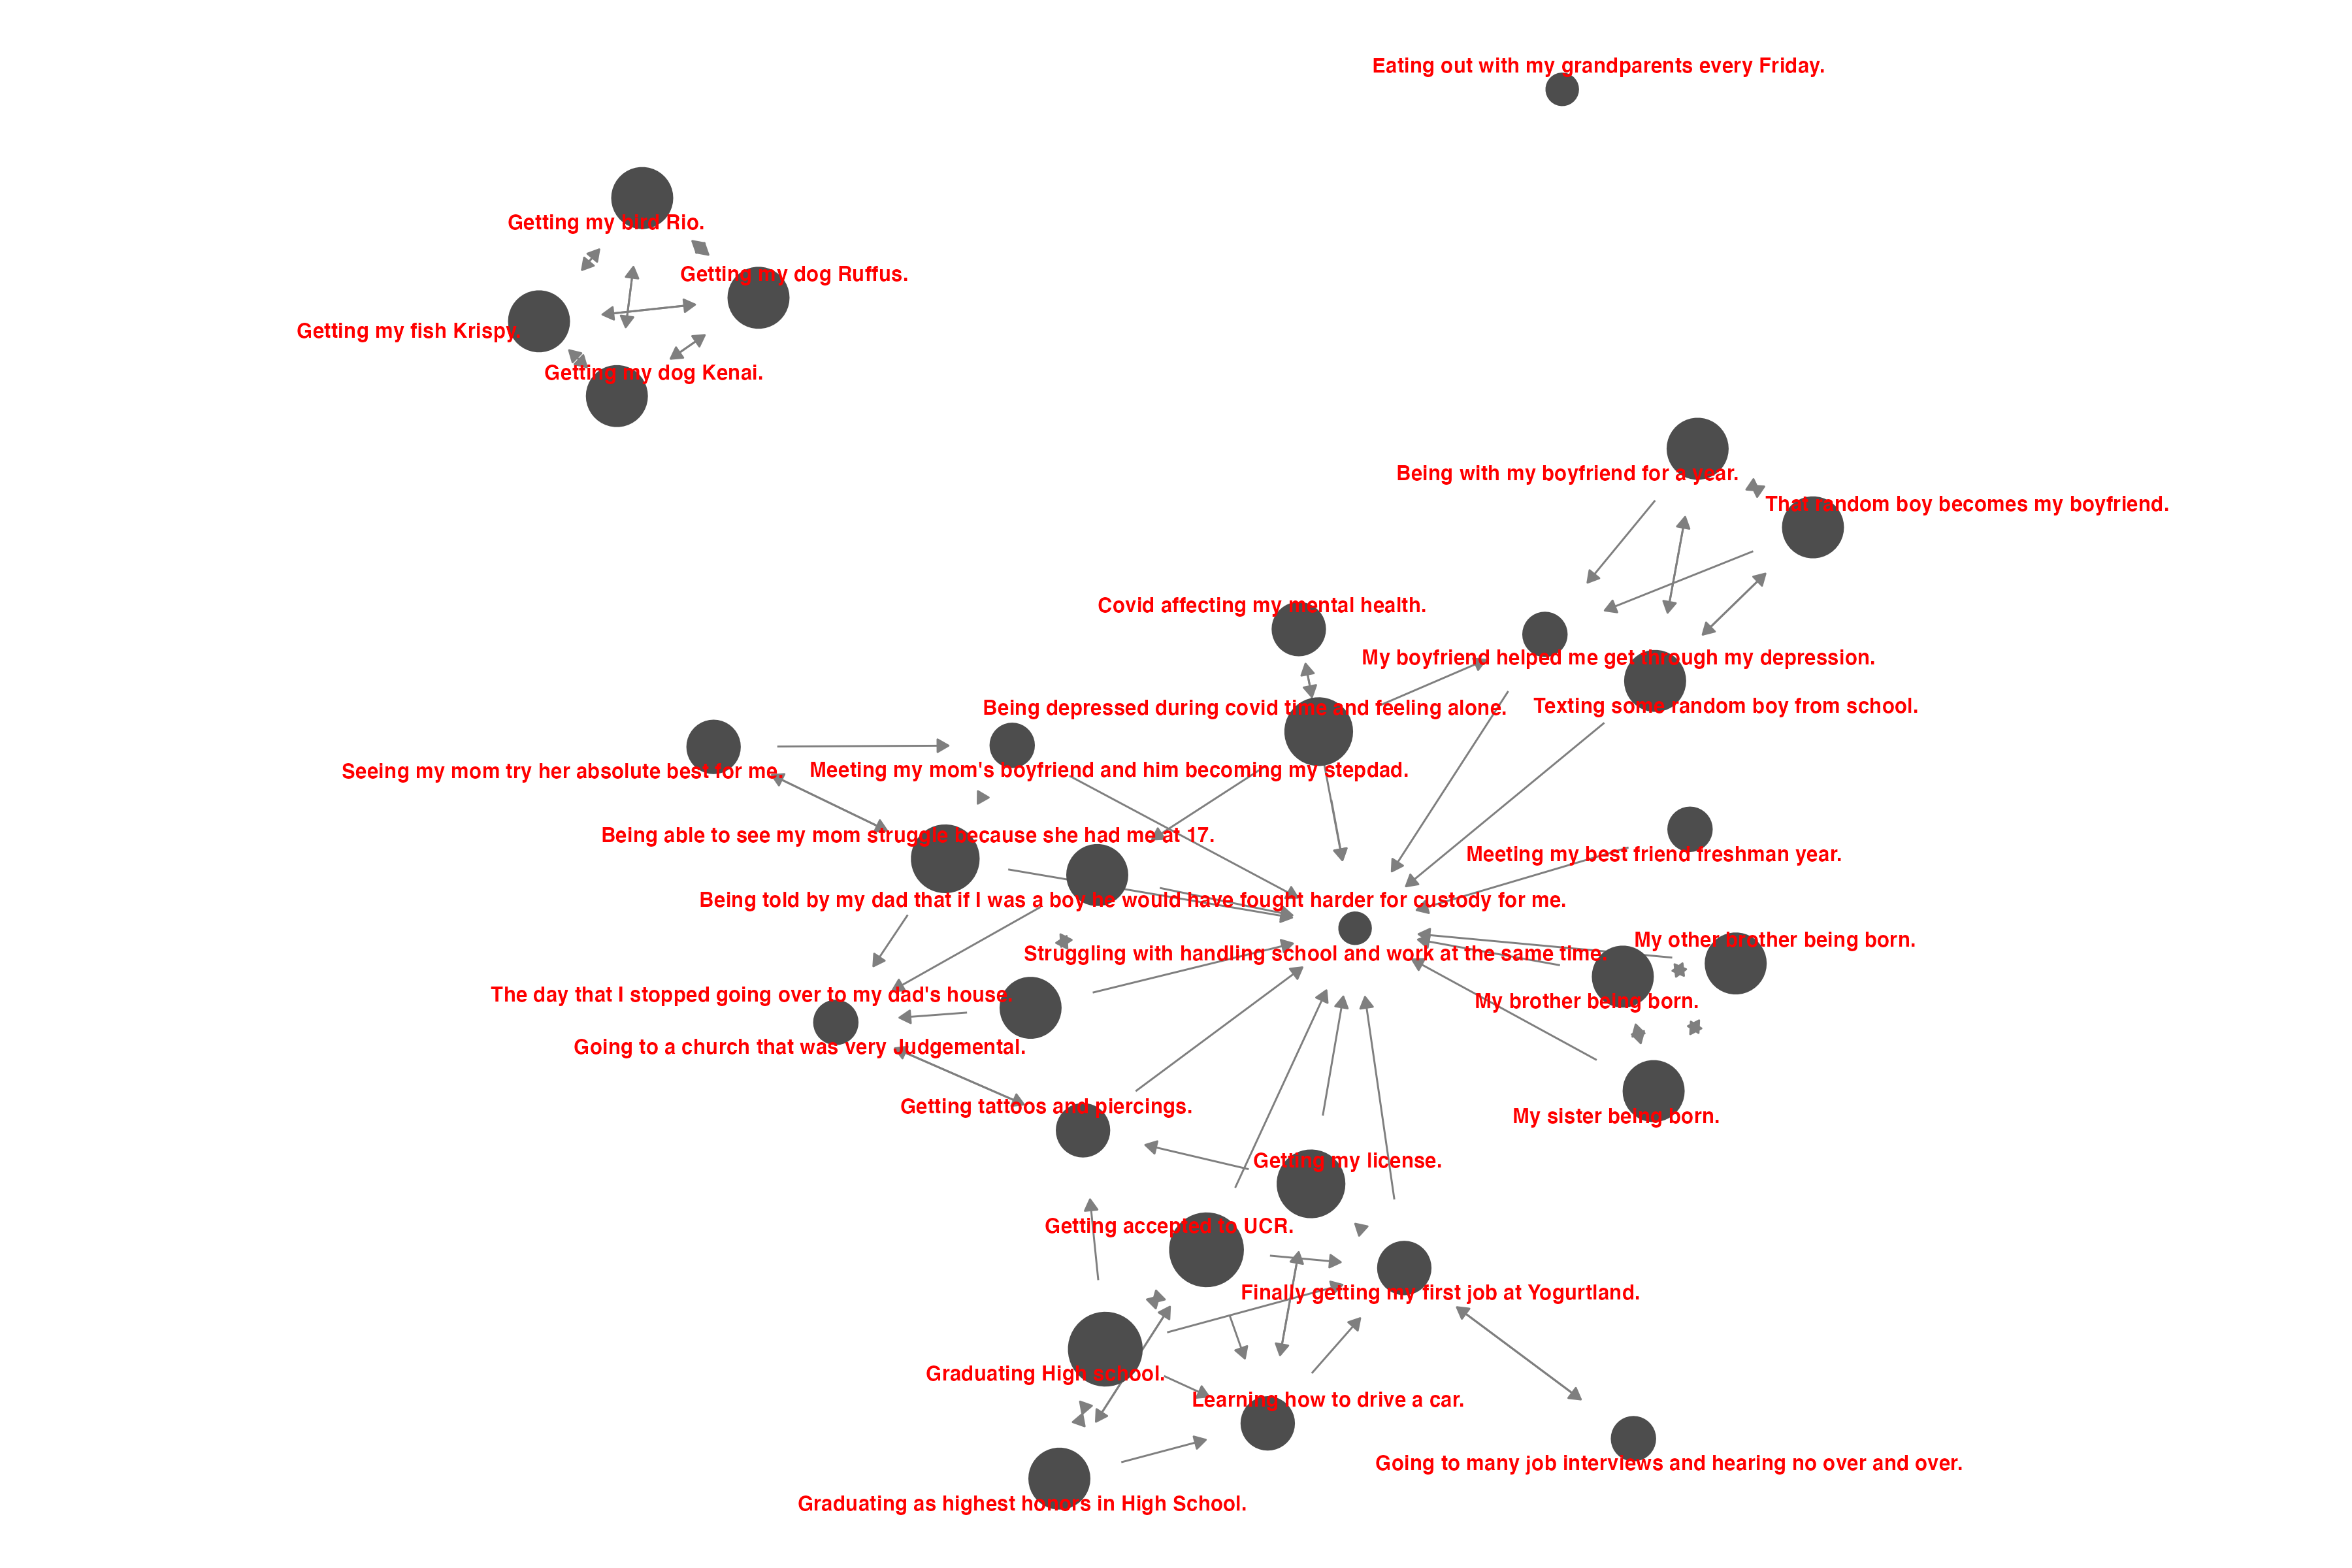
\includegraphics{images/61639_net.png}

\begin{center}\rule{0.5\linewidth}{0.5pt}\end{center}

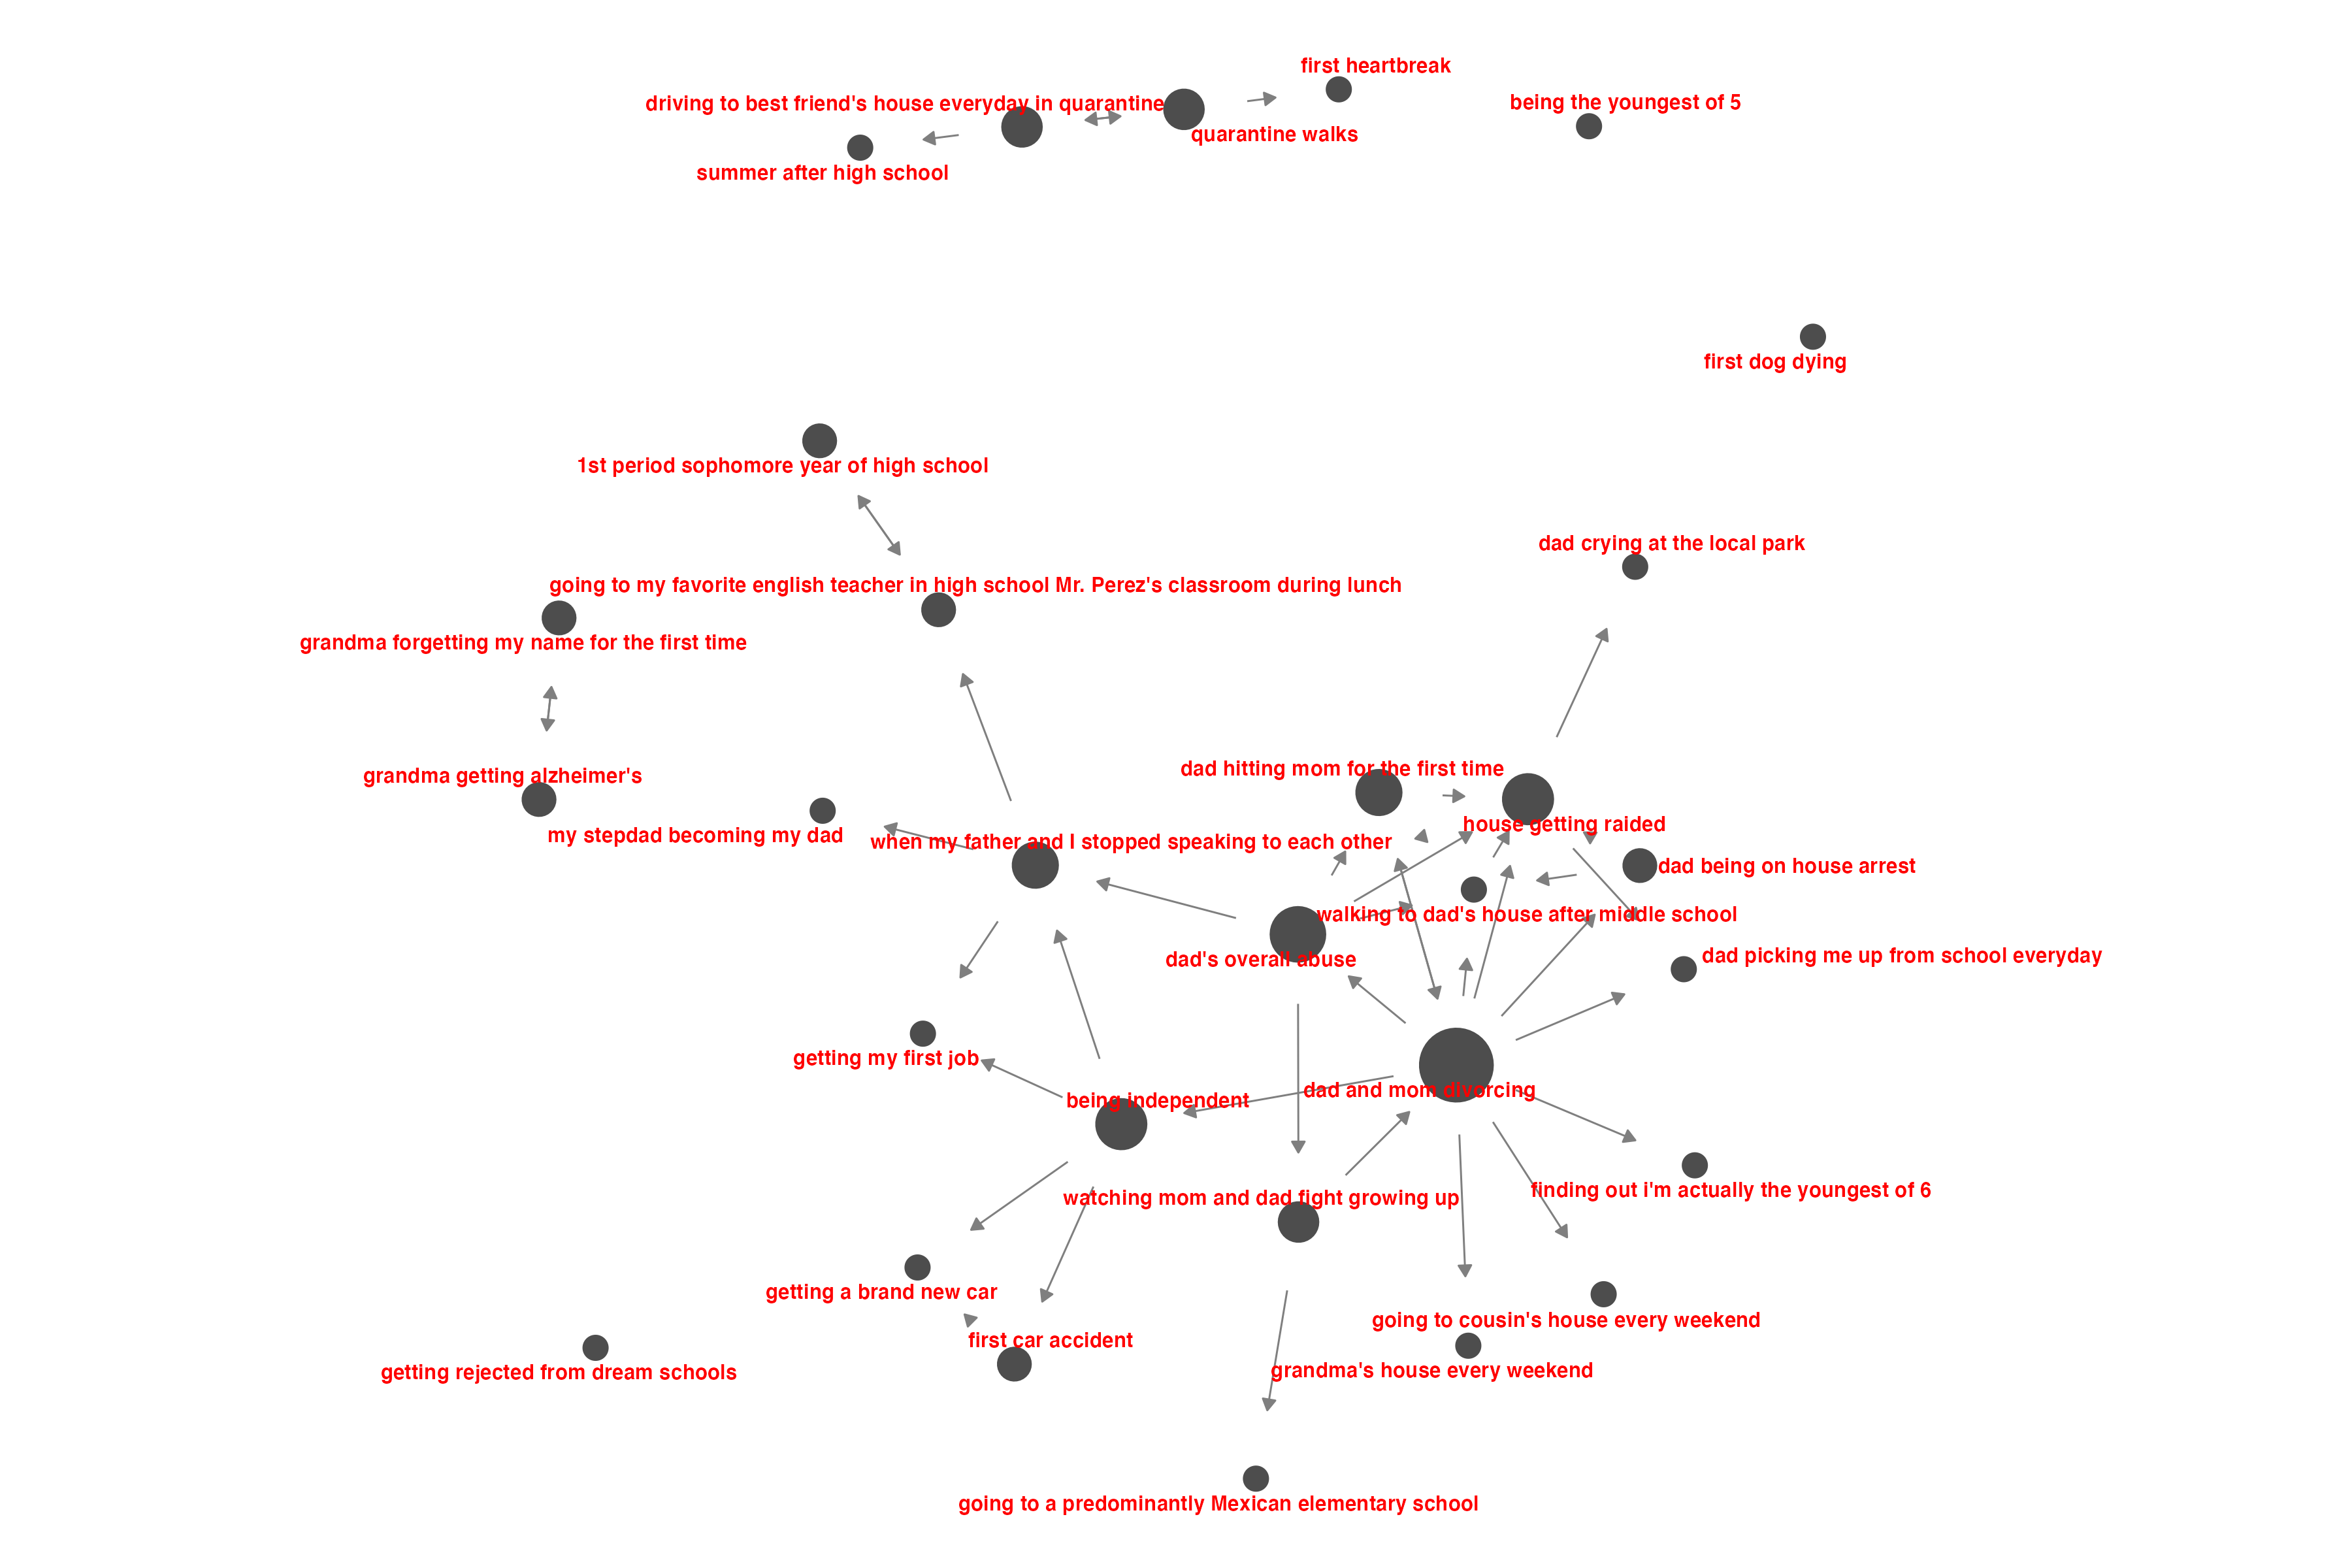
\includegraphics{images/61605_net.png}

\hypertarget{descriptives}{%
\section{Descriptives}\label{descriptives}}

\hypertarget{descriptives-for-outward-implications}{%
\subsection{Descriptives for Outward
Implications}\label{descriptives-for-outward-implications}}

\begin{verbatim}
   vars    n mean   sd median trimmed  mad min max range skew kurtosis   se
X1    1 3429 1.98 2.16      1    1.61 1.48   0  19    19 1.94     5.59 0.04
\end{verbatim}

\hypertarget{descriptives-for-inward-causes}{%
\subsection{Descriptives for Inward
Causes}\label{descriptives-for-inward-causes}}

\begin{verbatim}
   vars    n mean   sd median trimmed  mad min max range skew kurtosis   se
X1    1 3429 1.98 2.23      1     1.6 1.48   0  29    29 3.93    26.16 0.04
\end{verbatim}

\hypertarget{descriptives-for-number-of-words}{%
\subsection{Descriptives for Number of
Words}\label{descriptives-for-number-of-words}}

\begin{verbatim}
   vars    n  mean    sd median trimmed  mad min max range skew kurtosis  se
X1    1 3429 10.63 17.74      6    7.18 4.45   0 262   262 6.68     61.8 0.3
\end{verbatim}

\hypertarget{main-effects}{%
\section{Main Effects}\label{main-effects}}

\hypertarget{number-of-inward-causes-predict-positivity}{%
\subsection{Number of Inward Causes Predict
Positivity}\label{number-of-inward-causes-predict-positivity}}

\begin{verbatim}
Warning in checkConv(attr(opt, "derivs"), opt$par, ctrl = control$checkConv, :
Model failed to converge with max|grad| = 0.00227397 (tol = 0.002, component 1)
\end{verbatim}

\captionsetup[table]{labelformat=empty,skip=1pt}
\setlength{\LTpost}{0mm}
\begin{longtable}{lccc}
\toprule
\textbf{Characteristic} & \textbf{Beta} & \textbf{95\% CI}\textsuperscript{1} & \textbf{p-value} \\ 
\midrule
scale(outdegree) & -0.02 & -0.06, 0.03 & 0.4 \\ 
scale(indegree) & 0.07 & 0.02, 0.12 & 0.004 \\ 
numID & 0.00 & -0.01, 0.01 & 0.8 \\ 
scale(length) & -0.03 & -0.07, 0.01 & 0.094 \\ 
\bottomrule
\end{longtable}
\begin{minipage}{\linewidth}
\textsuperscript{1}CI = Confidence Interval\\
\end{minipage}

\begin{center}\rule{0.5\linewidth}{0.5pt}\end{center}

\begin{verbatim}
Warning: Some predictor variables are on very different scales: consider
rescaling
\end{verbatim}

\begin{verbatim}
Warning in checkConv(attr(opt, "derivs"), opt$par, ctrl = control$checkConv, :
Model failed to converge with max|grad| = 0.0022238 (tol = 0.002, component 1)
\end{verbatim}

\begin{verbatim}
Warning: Some predictor variables are on very different scales: consider
rescaling
\end{verbatim}

\begin{verbatim}
Scale for 'colour' is already present. Adding another scale for 'colour',
which will replace the existing scale.
\end{verbatim}

\begin{verbatim}
Scale for 'y' is already present. Adding another scale for 'y', which will
replace the existing scale.
\end{verbatim}

\begin{verbatim}
Warning: Removed 253 row(s) containing missing values (geom_path).
\end{verbatim}

\begin{verbatim}
Warning: Removed 253 row(s) containing missing values (geom_path).
\end{verbatim}

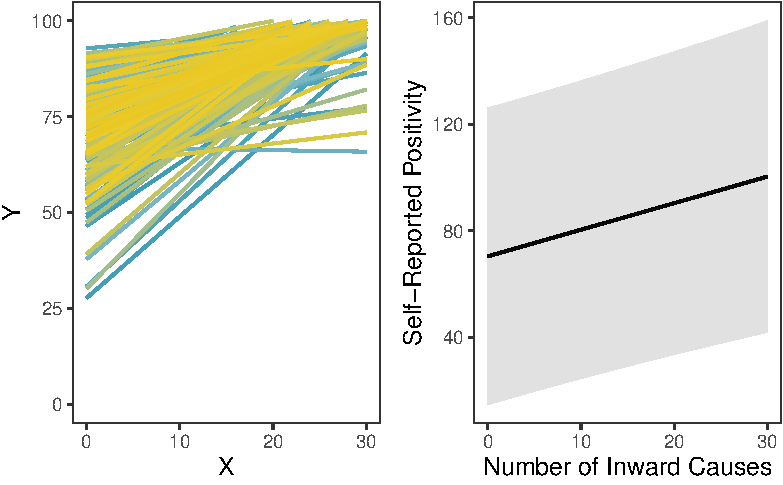
\includegraphics{EpMemNet_LabPres_htmldoc_files/figure-pdf/unnamed-chunk-8-1.pdf}

\begin{center}\rule{0.5\linewidth}{0.5pt}\end{center}

\hypertarget{no-effect-for-negativity}{%
\subsection{No Effect for Negativity}\label{no-effect-for-negativity}}

\begin{verbatim}
Warning in checkConv(attr(opt, "derivs"), opt$par, ctrl = control$checkConv, :
Model failed to converge with max|grad| = 0.00403987 (tol = 0.002, component 1)
\end{verbatim}

\captionsetup[table]{labelformat=empty,skip=1pt}
\setlength{\LTpost}{0mm}
\begin{longtable}{lccc}
\toprule
\textbf{Characteristic} & \textbf{Beta} & \textbf{95\% CI}\textsuperscript{1} & \textbf{p-value} \\ 
\midrule
outdegree & 0.38 & -0.41, 1.2 & 0.3 \\ 
indegree & -1.0 & -2.0, -0.03 & 0.043 \\ 
numID & 0.23 & -0.07, 0.53 & 0.13 \\ 
scale(length) & 0.39 & -1.2, 2.0 & 0.6 \\ 
\bottomrule
\end{longtable}
\begin{minipage}{\linewidth}
\textsuperscript{1}CI = Confidence Interval\\
\end{minipage}

\hypertarget{vader-classified-positive-sentiment}{%
\subsection{VADER Classified Positive
Sentiment}\label{vader-classified-positive-sentiment}}

\begin{table}
\centering
\begin{tabular}{l}
\hline
value\\
\hline
holidays\\
\hline
friends\\
\hline
Friends\\
\hline
celebrating holidays\\
\hline
Strong\\
\hline
Faith\\
\hline
Hope\\
\hline
Love\\
\hline
Careful\\
\hline
Successful\\
\hline
Openness\\
\hline
Kiss my lover\\
\hline
Celebrating my best friends birthday.\\
\hline
Ending friendship with best friend.\\
\hline
First love\\
\hline
First Love\\
\hline
cheerleading growing up\\
\hline
I love to laugh\\
\hline
Meeting my best friend\\
\hline
meeting my best friend\\
\hline
my first best friend\\
\hline
winning \$100\\
\hline
making friends\\
\hline
Toxic Friends\\
\hline
college acceptance\\
\hline
friendship breakup\\
\hline
Partying with my friends\\
\hline
first kiss\\
\hline
countless adventures with my good friends\\
\hline
first kiss\\
\hline
first kiss\\
\hline
first kiss\\
\hline
First Kiss (Stage kiss)\\
\hline
First kiss\\
\hline
first kiss\\
\hline
College acceptances\\
\hline
College acceptances\\
\hline
Katrina best high school friend\\
\hline
Play dates with my childhood best friend\\
\hline
Playing with my friends\\
\hline
playing fortnite with friends\\
\hline
Play snowball\\
\hline
Won the racing car award\\
\hline
Played soccer\\
\hline
Played tennis\\
\hline
Winning BIPOC award and scholarship.\\
\hline
Celebrated 18th birthday with friends\\
\hline
creating an original song\\
\hline
Winning my first research prize\\
\hline
Winning my first writing prize\\
\hline
Cheerleading Practice\\
\hline
GOD. JESUS. Feeling the Holy Spirit!\\
\hline
my first love\\
\hline
I love reading\\
\hline
losing my best friend\\
\hline
Eating delicious food\\
\hline
my kindergarten best friend moving away\\
\hline
My best friend moving to Oregon\\
\hline
finding my first real best friend\\
\hline
When my best friend passed away\\
\hline
Meeting my best friend freshman year.\\
\hline
My dog is my best friend\\
\hline
opening up to my best friend\\
\hline
celebrated 18th birthday\\
\hline
meeting my best friend from kindergarden\\
\hline
Hanging out with childhood best friends\\
\hline
telling my friends I love them\\
\hline
Graduating with my two best friends\\
\hline
Playing kickball\\
\hline
Playing minecraft\\
\hline
Playing soccer.\\
\hline
playing games\\
\hline
Creating a friend group that still holds strong\\
\hline
Striving to love harder everyday, stay brave, stay gentle, and keep forgiving. I am loved.\\
\hline
Winning Dionysus award in senior year\\
\hline
graduating with honors\\
\hline
Becoming a tia\\
\hline
becoming cheer captain\\
\hline
graduating highest honors\\
\hline
Winning championships in a basketball game\\
\hline
Playing soccer with my friends\\
\hline
Playing basketball with my friends\\
\hline
Playing Video Games with Friends\\
\hline
Playing video games with friends\\
\hline
winning a tournament with my friends\\
\hline
Falling in love\\
\hline
falling in love\\
\hline
Falling in love.\\
\hline
shopping with friend\\
\hline
meeting new friend\\
\hline
Making honor roll.\\
\hline
Switching friend groups\\
\hline
my college friends\\
\hline
My friends' intervention\\
\hline
making new friends\\
\hline
making new friends\\
\hline
beach with friends\\
\hline
626 with friends\\
\hline
mall with friends\\
\hline
gifts for friends\\
\hline
halloween with friends\\
\hline
photoshoot with friends\\
\hline
Skating with friends\\
\hline
meet my friends\\
\hline
Meeting New Friends\\
\hline
Met online friends\\
\hline
making new friends\\
\hline
playing with my neighbors and my childhood best friend\\
\hline
Bella's Sweet 16\\
\hline
acceptance to ucr\\
\hline
Acceptance to UCR\\
\hline
Becoming emotional support for friends throughout high school\\
\hline
My first kiss\\
\hline
My first kiss\\
\hline
play video game with my friend\\
\hline
my first kiss\\
\hline
My first kiss\\
\hline
Meeting my first love.\\
\hline
My first kiss\\
\hline
Play video games with friends online\\
\hline
having a party\\
\hline
Holiday get togethers\\
\hline
First healthy relationship.\\
\hline
Losing my best friend senior year\\
\hline
Playing with Webkinz at a sleepover with my best friend\\
\hline
Having the best senior year and being happy\\
\hline
Promoting 8th grade\\
\hline
Fighting friends\\
\hline
Stuck in the slide with best friend\\
\hline
My best friend dropping me for his girlfriend\\
\hline
My best friend moving to a different state.\\
\hline
Reconnecting with my childhood best friend freshman year.\\
\hline
Playing video games with my friends\\
\hline
Playing video games with new friends\\
\hline
playing fortnite with my close friends\\
\hline
Going to the gym and gaining confidence\\
\hline
First feeling of improvement in things I cared about\\
\hline
My current friend group sharing deep secrets\\
\hline
Playing with my favorite stuffed animal.\\
\hline
Finding out my best friend had serious issues.\\
\hline
Growing up playing with boys\\
\hline
Getting into beef to protect my friend\\
\hline
Became choir president, which boosted by confidence.\\
\hline
Celebrate my friend Step's 18 birthday in Boston\\
\hline
Watching movie ""Smile"" with my friend Irene\\
\hline
No longer became friends with my best friend in high school\\
\hline
Winning my first race\\
\hline
Winning a swim competition\\
\hline
The day my best friend died\\
\hline
Getting made fun of\\
\hline
leading my cheer team\\
\hline
becoming varsity cheer captain\\
\hline
Made the cheer team\\
\hline
winning my first medal from a sport (swimming)\\
\hline
Overcoming many obstacles, but now feeling better and a bit accomplished.\\
\hline
Meeting my first friend\\
\hline
Drama with friend groups\\
\hline
Making my first friend.\\
\hline
Go concert with friend\\
\hline
Being with my best friend everyday of the summer.\\
\hline
I was the therapist friend, because I liked helping friends with their problems.\\
\hline
My ""best friend"" hooking up with my ""almost boyfriend""\\
\hline
When I met my best friend in 4th grade.\\
\hline
I won a basketball 1v1 and won a dollar.\\
\hline
Finding my love for music\\
\hline
Committed to UCR\\
\hline
Learning how to love Myself\\
\hline
Finding YouTube channels I love\\
\hline
getting the dog i love\\
\hline
My friends surprising me on my birthday\\
\hline
Going to my first concert with my best friends.\\
\hline
handout with my friends\\
\hline
Stay at friends home\\
\hline
Eating food with friends\\
\hline
Hoola Hooping with friends\\
\hline
Snowboard trip with friends\\
\hline
Meeting My Lifelong Friends\\
\hline
First Friendsgiving with friends\\
\hline
Making friends in college\\
\hline
friends and family influence\\
\hline
Made many new friends\\
\hline
made life long friends\\
\hline
Meeting My College Friends\\
\hline
I have many friends\\
\hline
gymming with different friends\\
\hline
My great grandma passing away.\\
\hline
Receiving college acceptance letters.\\
\hline
working at sweet rendezvous\\
\hline
Playing bass for my worship group\\
\hline
Discovering my favorite anime\\
\hline
Getting awards and recogintions\\
\hline
Being happy within myself !\\
\hline
playing basketball with my life long friends\\
\hline
Getting accepted to my top colleges\\
\hline
Getting accepted to my top college\\
\hline
I got good grades\\
\hline
I ate good food\\
\hline
Mother always supporting me\\
\hline
Starting my first cheer competition and winning second place.\\
\hline
becoming a cheerleader\\
\hline
starting high school with high and strong motivation\\
\hline
promoted from middle school\\
\hline
Visiting my best friend at her college, which is UCI.\\
\hline
I was out in Tijuana with my other best friend.\\
\hline
Meeting my best friends that I made in high school\\
\hline
My best friend almost dying in an accident\\
\hline
losing my first love\\
\hline
My first romantic relationship\\
\hline
my first college party\\
\hline
my 18th birthday party\\
\hline
My 15 birthday party\\
\hline
My 5th birthday party\\
\hline
Starting playing soccer\\
\hline
Playing team sports\\
\hline
winning a prize in a giveaway and my two ""best friends"" took the prize and didn't invite me over to use it with them\\
\hline
Problem Solving\\
\hline
Made 3 free throws to win a Varsity basketball game\\
\hline
Lost touch with childhood best friends in high school\\
\hline
Maintaining long term friendships\\
\hline
Got a credit card\\
\hline
Realizing I like being active and am athletic\\
\hline
Celebrated Chinese Lunar new year with friends in Hong Kong\\
\hline
Winning my first badminton tournament\\
\hline
Growing up christian\\
\hline
winning my first tennis tournament\\
\hline
Hip-Hop Competitive Dance\\
\hline
Getting my wisdom teeth removed.\\
\hline
Meeting the Love of My Life\\
\hline
experiencing love for the first time\\
\hline
join the Pomona College Academy for Youth Success program\\
\hline
Breaking up with my first love.\\
\hline
Promoting from Middle School\\
\hline
Promoting to High School\\
\hline
Receiving high honors throughout school\\
\hline
First time become honors student\\
\hline
visiting my great grandfather with Alzheimers\\
\hline
W/my best childhood friend: Dulani -- call each other ""sisters"" tdy\\
\hline
Having a Great 4/5th Grade Teacher\\
\hline
First lecture. went really well and I loved my professor!\\
\hline
my best friend getting hospitalized for months when we were six\\
\hline
playing video games with my friends every weekend\\
\hline
Devoting time to playing tennis throughout high school\\
\hline
playing basketball with my friends at rec centers\\
\hline
Playing tag with my friends at the playground\\
\hline
hanging out with friends all nighters playing games\\
\hline
Grad night having a fun night with my friends for like the last time\\
\hline
Being told by my friends that I'm a good listener and give good advice\\
\hline
When I first fell in love but learned that it wasn’t really love\\
\hline
Giving CPR to someone\\
\hline
festival at church at night\\
\hline
giving my commencement speech\\
\hline
my dad becoming my friend\\
\hline
Great times with my beautiful grandma and grandpa when I was young\\
\hline
My senior year friend group\\
\hline
Visiting my friend at Vegas\\
\hline
Breaking my wrist and hand.\\
\hline
Firsttime go boba w friend\\
\hline
Resolving a conflict\\
\hline
I remember winning the CIF championship for our tennis team.\\
\hline
being in competitive cheerleading for four years\\
\hline
Took yoga class with friends\\
\hline
Standing up for my friends\\
\hline
Making new friends after highschool.\\
\hline
Making new friends in college\\
\hline
making friends in elementary school\\
\hline
Watching a movie with friends\\
\hline
Made friends in high school\\
\hline
Going to L.A. with friends\\
\hline
First secret Santa with friends\\
\hline
Meeting my close childhood friends\\
\hline
Make friends in middle school\\
\hline
Making friends on my own\\
\hline
Going to Disneyland with friends\\
\hline
Criminal Justice class\\
\hline
Celebrating my graduation and realizing how proud people were of me.\\
\hline
Getting awards for my gpa\\
\hline
Receiving my UCR acceptance letter\\
\hline
Becoming best friends with a girl who I mutually disliked\\
\hline
Watching my favorite tv show\\
\hline
Joined High School Girl's basketball and got a confidence boost\\
\hline
Random lady called me cute\\
\hline
gaming and interest in tech\\
\hline
my friends really helping me through my struggles\\
\hline
Moving to Arkansas beginning of 9th grade and leaving my best friend\\
\hline
I was skating the streets of Seattle at midnight with best friend.\\
\hline
celebrating my first birthday in America\\
\hline
The loss of a soulmate\\
\hline
throwing my mom a surprise party and seeing the smile on her face\\
\hline
doing good on a test\\
\hline
Dying my hair bright red.\\
\hline
Hanging out with my best friends before we all leave for college.\\
\hline
Playing with my childhood friend when we were kids\\
\hline
Meeting Brandon, who was my first love\\
\hline
Getting accepted to colleges.\\
\hline
Getting accepted into college\\
\hline
getting accepted to college\\
\hline
getting accepted to UCR\\
\hline
Getting accepted into college\\
\hline
Getting accepted to UCR\\
\hline
getting accepted into college\\
\hline
Getting accepted to UCR.\\
\hline
Being Accepted into Universities\\
\hline
Playing video games with my friends on the weekends\\
\hline
Playing pickup basketball at the park with my friends\\
\hline
Got accepted into UCR\\
\hline
walking to Pizza Love with my brothers\\
\hline
Getting accepted into college\\
\hline
get accepted into colleges\\
\hline
Becoming a God mommy.\\
\hline
Sharing food with my girlfriend\\
\hline
Losing my first friend\\
\hline
Fighting with my friends\\
\hline
Winning competitions in kendo and kendama\\
\hline
Enjoying tacos and a local shop\\
\hline
going to my first party\\
\hline
Having a party at home\\
\hline
Feeling loved by everyone around me in my highschool graduation\\
\hline
winning a reading contest and getting free tickets to an A's game\\
\hline
I found friends that made me become a better person, socially\\
\hline
Treat people how you want to be treated\\
\hline
Getting cast as a supportive character in highschool play\\
\hline
Doing really well on triple jump and my coach praising me.\\
\hline
Sharing a hotel room with two other friends for a convention\\
\hline
First time a child hugged me (my baby cousin) - made me feel warm and loved\\
\hline
Partying for the first time\\
\hline
Had my first ever crush in kindergarten. I learned that liking people romantically could be fun.\\
\hline
Went to night markets with friend\\
\hline
My first sleepover with my friend\\
\hline
Went to ski with my friend\\
\hline
Kicking a guy's genitals because they were making fun of my friends.\\
\hline
Meeting first close friend in highschool\\
\hline
Getting close with my friend Claire\\
\hline
Go to the beach with friend\\
\hline
Filming romeo and juliet with friend\\
\hline
Going to Newport to look at the beautiful houses to get motivation.\\
\hline
Getting cheated on lol\\
\hline
Making my first Survivor audition.\\
\hline
Training at a fitness boot camp to improve my health\\
\hline
Went to Philippine with friends twice\\
\hline
Wen to a concert with friends\\
\hline
Going to the beach with friends\\
\hline
Making new friends in 7th grade\\
\hline
Meeting my roommate and college friends\\
\hline
Renting a theatre with my friends\\
\hline
Wanting white friends in middle school\\
\hline
Watching my friends do long distance\\
\hline
Hanging out with family and friends.\\
\hline
Friends I made at my jobs\\
\hline
making friends at a new school\\
\hline
Getting boba afterschool with my friends\\
\hline
First friends made in elementary school\\
\hline
Going to Lake Havasu with my friends and getting tan and being happy\\
\hline
Being dropped by someone I considered my best friend and never being told why.\\
\hline
Having a really a strong friendship throughout elementary to end of middle school\\
\hline
Driving on the freeway by myself and making it to my destination safely, giving me more confidence to drive by myself.\\
\hline
Felt hopeless and very hurt from friendships and love\\
\hline
driving to best friend's house everyday in quarantine\\
\hline
Playing with my brother\\
\hline
playing family at preschool\\
\hline
my acceptance letters to the universities\\
\hline
Learning how to play piano\\
\hline
playing basketball in league\\
\hline
learning to play the cello\\
\hline
Watching my favorite movie in theaters\\
\hline
Playing with video games.\\
\hline
My 4th relationship - positive self reflection\\
\hline
Learning how to play soccer\\
\hline
Favorite toys were Pokemon, Bakugan, Beyblade\\
\hline
Playing the videogame ""Valorant""\\
\hline
Knowing how to play violin\\
\hline
Helping my cousins after they left a toxic family dynamic\\
\hline
Getting my first college acceptance letter.\\
\hline
feeling weird around friends because they wanted to drink\\
\hline
working at a boba shop for one day to help my friend\\
\hline
Watching my great aunt pass in the hospital\\
\hline
First time receive the Essay writing award\\
\hline
Grad Nite at California Adventure\\
\hline
when my friend died\\
\hline
Growing up with cousins\\
\hline
Worked at Amazon warehouse\\
\hline
Growing up in Chicago\\
\hline
Receiving most valuable athlete in high school.\\
\hline
I met one of my childhood best friends at my birthday in my early years\\
\hline
Playing hide and seek with my friends in the backyard.\\
\hline
Learning that I must depend and trust others in order to better myself.\\
\hline
having my first kiss at 13\\
\hline
Gaining close relationships with my siblings\\
\hline
Sharing a room with my roommate\\
\hline
Performed in middle school talent show\\
\hline
Get lucky money and buy toys\\
\hline
My siblings doing random things for fun\\
\hline
Going to my very first college party with my newly made college friends.\\
\hline
Becoming a Tia to my first niece.\\
\hline
Graduating as highest honors in High School.\\
\hline
helping my cat give birth\\
\hline
Starting senior year and being cheer captain\\
\hline
The time my best friend sexually harassed my current girlfriend behind my back\\
\hline
Playing hopscotch on the sidewalk with my friends in the summer\\
\hline
I told people I played piano and they made me play for our graduating class talent show.\\
\hline
Having a boxing match with a friend for fun before he left for college.\\
\hline
watching my boyfriend follow his dreams\\
\hline
My first High School House party\\
\hline
One of my favorite activities to play in Elementary Schools was punchball\\
\hline
Learning more about a subject I enjoy.\\
\hline
Graduating High school in the honor role\\
\hline
Being left out by a friend group\\
\hline
Tomb-Sweeping Day (Qing Ming festival) in 2010\\
\hline
when friends car  broke down\\
\hline
The day I made my first friend\\
\hline
Finding my childhood friend after many years.\\
\hline
enjoy the last bit of senior year\\
\hline
Discourse with my high school friend group\\
\hline
taking care of kids in afterschool program\\
\hline
Being very good at socializing at school\\
\hline
Getting high with my cousins during Christmas and having one the best laughs I've ever had\\
\hline
Being accepted into 6 Universities\\
\hline
Getting accepted to 7 colleges\\
\hline
learning how to love myself at a young age\\
\hline
Seeing my mom try her absolute best for me.\\
\hline
getting accepted into a UC\\
\hline
I made love to a Russian prostitute in Moscow\\
\hline
Visiting my best friend's house for the first time\\
\hline
My dad hit me for discipline, made me question father role, love, and God.\\
\hline
Listening to the stories of my parent's love story\\
\hline
Family coming over for the holidays\\
\hline
Going to knott's berry farm with friends\\
\hline
Sneaking into my friends house at night\\
\hline
Participated Leadership program with friends in 2019\\
\hline
Lived in Boston University dormitory with friends\\
\hline
Team building exercises with friends during camp\\
\hline
I remember graduating alongside all my friends.\\
\hline
reconnecting with my old elementary school friends\\
\hline
making new friends in this new environment\\
\hline
Proofread college essays for my underclassmen friends\\
\hline
camping with my friends in my backyard\\
\hline
Traveling to Hawaii with my closest friends\\
\hline
biking to the beach with my friends\\
\hline
Go coffee to do hw with friends\\
\hline
Being talk behind the back by friends\\
\hline
Having a christmas week witth my friends\\
\hline
I was in 8th grade, me and my best friend at the time were going back home and I remember we always laughed and had a good time, I remember this because it was a happy pure memory\\
\hline
Grad night as Disneyland. Was extremely fun and chaotic, one last time to say goodbye and have fun with friends.\\
\hline
Graduating from ELA. I was so happy to finish the English learners program in fourth grade and I remember my teacher jumping, screaming, and hugging me with joy because she was really happy for me and I felt proud of myself to have accomplished that.\\
\hline
First frat party at ucla during halloween. really fun although extremely chaotic\\
\hline
Receiving awards from my team and school.\\
\hline
Only having myself when my best friends broke up with me for a few months\\
\hline
I remember as a young child playing Mario Party with my cousins. I remember just having so much fun and laughing with everyone over the smallest things.\\
\hline
I got accepted into all-stars softball after years of playing\\
\hline
Losing love for reading and books in highschool\\
\hline
Loving the lab scenes in Law and Order: SVU\\
\hline
Having really strong friendship, but few, in middle and high school\\
\hline
Winning a poetry recitation contest in elementary school.\\
\hline
First time I score a game winning shot\\
\hline
I found I was good at math\\
\hline
Transferring colleges to play volleyball again\\
\hline
i played waterpolo, soccer, swim, dance\\
\hline
Played basketball for middle school team\\
\hline
Reconnected with my brother after many years of hating each other, we're now best friends.\\
\hline
Getting my first straight A's\\
\hline
Getting straight A's in college.\\
\hline
I remember the girl with the huge breasts that I was fond of.\\
\hline
losing my friends in middle school\\
\hline
The arabic show. We do this show every year for my arabic class and the first year was so fun, I met two of my other best friends and we practiced doing traditional dances, songs, and plays. It was so fun and I felt super connected to my culture and felt like those around me were like my family in that class.\\
\hline
I did cheer in freshmen of high school\\
\hline
When I graduated high school with high honors\\
\hline
Hanging out with my sister and having fun\\
\hline
Helping Ashley with her anxiety\\
\hline
Had my first boyfriend, he broke up with me because of his new girl best friend.\\
\hline
Getting my first kiss outside my house\\
\hline
Rejecting a guy I liked\\
\hline
When i got an important character in 4th grade choir play\\
\hline
gaining large amounts of weight in highschool\\
\hline
Go to high school at United state\\
\hline
Buying my first lip product and realizing I love lipstick/chapstick.\\
\hline
Learned to love again and heal after meeting current boyfriend.\\
\hline
Enjoying some unexpected time alone more compared to going out all the time with friends\\
\hline
Became a Lakers fan in 2009\\
\hline
Meeting an online friend for the first time\\
\hline
getting an apartment with my boyfriend and friend\\
\hline
Became an Iworker and took care of kids\\
\hline
My mom getting cancer in 7th grade (but survived)\\
\hline
My great grandpa taught me how to ride a bike\\
\hline
Playing sports with my family\\
\hline
Deciding to quit playing soccer.\\
\hline
playing my first video game\\
\hline
Important conversations with my mom\\
\hline
playing basketball in middle school\\
\hline
My 21st birthday party at my house\\
\hline
Playing video games with cousins\\
\hline
Playing tetherball during the summer.\\
\hline
Playing with my cousins basketball\\
\hline
playing dolls in my room\\
\hline
getting help from my siblings with homework\\
\hline
Got into my first ""relationship"" which was confusing, weird, but ultimately made me realize that guys do think I'm pretty and I'm lovable\\
\hline
My favorite childhood toys to play with were Legos, Nerf blasters, and  Yu-Gi-Oh cards\\
\hline
playing basketball with my dad\\
\hline
playing soccer as a kid\\
\hline
playing baseball as a kid\\
\hline
coming to the United States confused\\
\hline
Having personal conversations with my two closest friends\\
\hline
Going to New York with three other friends\\
\hline
driving my friends around for the first time\\
\hline
Investing in buying shoes, because that would make me happy!\\
\hline
When I realized who my real friends were\\
\hline
My first sleep over at my friends house\\
\hline
Recording my first song in my friends basement\\
\hline
When me and my sister finally became friends\\
\hline
Going on late night drives with my friends\\
\hline
My parents saying they are proud of me\\
\hline
Moving away from my hometown and childhood friends.\\
\hline
Meeting some of my current friends in college.\\
\hline
my sister helping me with everything\\
\hline
Late night phone calls with my best friend over how depressed and lonely we are\\
\hline
Experiencing my first loss of a friend\\
\hline
My eighth memory was when I reviewed my first piano as a gift from my father. I was self taught and value my talent to play it today\\
\hline
Winning county mock trial the first time\\
\hline
Reaching ""Supreme"" (one of the highest ranks) in Counter Strike: Global Offensive\\
\hline
The first time I kissed a female\\
\hline
Being in toxic friendships throughout middle school\\
\hline
Committing to a college\\
\hline
I played my first recital in years after the passing of my previous cello teacher in 2019. Through this, I gained a great amount of confidence and reignited my passions for my instrument after a long period of wanting to quit.\\
\hline
My lifting journey, a year and a half strong continuously making massive strides in hypertrophy and strength\\
\hline
This girl I liked, I knew she liked someone else, and that completely changed me.\\
\hline
Lost contact with my best friends and started feeling lonely and upset that I didn't choose the right school\\
\hline
Convincing my dad to get me a speed racer novel that I never read, I thought the title looked cool\\
\hline
When my favorite teacher in middle school moved\\
\hline
Watching my favorite cartoon shows on weekend mornings.\\
\hline
Gathering life lessons and virtues from the music and experiences of my grandparents, parents and their friends. Extremely important to me.\\
\hline
Growing up in an apartment\\
\hline
first time winning a high level tennis tournament (L3)\\
\hline
competing and winning fastest swimmer for my age division\\
\hline
Winning first place at my gymnastics meet in Texas\\
\hline
My 1st best friend in elementary school threatened to choke me out in 6th grade.\\
\hline
Being fascinated with games ever since I've seen my family play with the Nintendo DS.\\
\hline
When I was shown actual love and found the person I want to be with\\
\hline
Felt insecure when I was with my friendgroup who I thought were all super skinny and pretty\\
\hline
Working out for the first time on a consistive schedule. It made me feel so powerful and good about myself! It helped me learn to love my body and associate working out and being health with positive feelings.\\
\hline
fight with friend night before leaving taiwan\\
\hline
When I got accepted into universities\\
\hline
Getting accepted to and attending college.\\
\hline
Falling out with a friend in junior year\\
\hline
I also remember going to my first Ram's game. We lost against the Balitomore Ravens but It was fun to experience. Just me and my dad went and I felt so happy just enjoying the moment with him.\\
\hline
Friend tried to kill themself\\
\hline
Always felt like to each their own\\
\hline
Learning how to get better at a game\\
\hline
first day of high school. I felt really nervous but I was really excited as well, and I got closer with someone who I knew from middle school but was not super close to and now were still best friends.\\
\hline
I won a few piano recitals back in elementary school\\
\hline
making my parents happy when I showed them my grades\\
\hline
Getting my first job and being promoted to manager, felt like someone finally believed me\\
\hline
Playing madden mobile with my friends at school and learning how to monetize it\\
\hline
When I was in grade school, like elementary level, I would wake up early to make my dad coffee because he would be happy and praise me.\\
\hline
Met a new friend group halfway through high school who made me genuinely happy and understood my home situation.\\
\hline
Reconnected with my faith and gave me hope as to where I was going with life.\\
\hline
The death of a close friend\\
\hline
During the month of september on President's day weekend, Arizona has a soccer competition for the leagues to enter and compete. It is the Laughlin tournament. It is really fun but also super cold. I would go every year when I used to play. It was a super fun weekend and I loved that my parents would always take me even if it meant they couldn't rest that specific weekend.\\
\hline
getting a drive from a friend met in class\\
\hline
Making my promposal for my ex with my friend\\
\hline
Eating with my family together and laughing with them\\
\hline
Deciding to go to a festival the day of\\
\hline
Taking care of my siblings at a young age\\
\hline
When I was with my childhood friend watching fireworks\\
\hline
Taking care of cats that lived under the house\\
\hline
Grad night in middle school. I had a lot of fun and got to go on rides at six flags with my friends and laugh all night together.\\
\hline
The first time that I played tennis\\
\hline
Going to the Maria clara festival with my grandma\\
\hline
the moment i saw progress at the gym\\
\hline
First time play sport at college level\\
\hline
Try to go to the birthday of many friend\\
\hline
Play piano by myself in 1 year\\
\hline
My high school gradation was a huge milestone for me. I had felt extremely accomplished and relieved to have finished high school, especially IB.\\
\hline
Went to church to watch my dad play volleyball and eventually I started playing and continued to teach myself how to play and get better through the years\\
\hline
Making the wrong decision with a friend\\
\hline
Having one of my best friends say he hated me when he first met me because I didn't laugh at his joke.\\
\hline
Being humbled by the abilities of my peers, older friends, my homelands, and random individuals.\\
\hline
Starting freshman year of college, I became much more ambitious and focused a lot more in my studies\\
\hline
My Grandpa saying that we are beautiful family at Sunday dinners\\
\hline
While I hate my ex now, I remember being first asked out after our choir performances. It taught me how you can connect with someone with similar initial interests and what first love felt like. However, our couple of breakups, the reasons why, and my nights of crying to sleep (sometimes even during work shifts) really taught me what an unhealthy relationship looked like and what values I truly wanted (honesty not out of controlling but out of just respect and that deep friend connection, similar/the same conceptualizations of what cheating is, true inclusivity in shared friend groups (not just tolerance), prioritization in deep conversations (not solely just in giving gifts, physical affection, and dates. I wanted a balance in love languages), healthy work/life boundaries (aka respecting no call times during school/work), and the same future goals (Ex: marriage, no children but pets, etc.) as well as open-mindedness to differing political beliefs.\\
\hline
moving into college and having to meet new friends\\
\hline
Meeting my High School friends for the first time\\
\hline
Being taught how work is valuable and work ethic\\
\hline
Moving to a high-school away from my existing friends\\
\hline
Saying bye to my friends at school in Brazil\\
\hline
Starting school in Sacramento, trying to make new friends.\\
\hline
Meeting new friends in High school and Elementary School\\
\hline
Go traveled around the world during every holiday\\
\hline
first romantic experience with a girl from volleyball\\
\hline
First romantic relationship in college and the end\\
\hline
Get sick and mom take care of\\
\hline
When I started my first sport and found a love for basketball\\
\hline
Going to the park with my middle school friends and playing on the monkey bars\\
\hline
Graduation, such a surreal feeling\\
\hline
Dressing up as Beowulf characters for extra credit\\
\hline
Helping my father with cleaning the house\\
\hline
Getting made fun of my asian lunch in elementary school\\
\hline
Living in LA county made me outgoing\\
\hline
I used to go swimming at my old best friend's house all the time before me and her stopped being friends.\\
\hline
Getting appendicitis - made me create more healthy habits, watch what I eat, be more hygienic\\
\hline
Seeing my friends go through bad experiences\\
\hline
Painting a lot a learning how to do better\\
\hline
When I first started playing volleyball\\
\hline
playing basketball every day after school\\
\hline
playing basketball with strangers every week\\
\hline
Playing video games with my brother\\
\hline
Playing video games with my brother\\
\hline
Playing with my toy train collection.\\
\hline
hitting with top professional tennis players\\
\hline
Losing contact with my friends from high school\\
\hline
When my best friend's mom took us to a doctor's science fair. It was for us to see if we would like to be in the medical field.\\
\hline
Falling in love for the first time - realizing the extent to how much I could care about someone who wasn't family\\
\hline
having a really strong group I could talk to about anything\\
\hline
Obsessing over my Nintendo DS and playing games like Cooking Mama and one where it was like a math game and the dude's head is huge and floating.\\
\hline
I like to take pictures to record life\\
\hline
Running into a friend I haven't seen in a while\\
\hline
My 7th grade and 8th grade friend group breaking up\\
\hline
getting my first real friend group in jr year highschool\\
\hline
My friend telling me about his endeavors with a girl\\
\hline
Got super burnt out trying to manage too many extracurriculars and school\\
\hline
I remember in middle school some of my friends and I went to a friend’s house to hang out and play some games together. I remember having a good time, laughing and screaming with everyone.\\
\hline
My third memory happens to be in second grade when my best friend from kindergarten in which I have not seen since then came to visit me in class.This moment might have been the greatest satisfaction of having to see someone for a long time.\\
\hline
Entering college - scared but also eager after seeing how large the campus was and the workload and amount of learning needed to be successful\\
\hline
Taking ‘Transpersonal Psychology’ in high school, which definitely helped with my perception of myself and self growth.\\
\hline
losing a friend to suicide\\
\hline
Suffered because of math, it constantly degraded my self importance and value.\\
\hline
Understanding that, whatever happens happens. I can only try and do my best.\\
\hline
I sang in the yearly talent show every year.\\
\hline
Win the election and be the president of high school student council.\\
\hline
my first college match, playing singles when we traveled and my parents came to support.\\
\hline
My dad used to always want me to play basketball as a child but I would get nervous and embarassed. I chose to play soccer and I ended up loving it, and so did he.\\
\hline
I joined the football team where I met close friends.\\
\hline
Going to the beach and having a bonfire with friends.\\
\hline
Having a comeback when someone said something mean to me in middle school and then becoming friends with his friends.\\
\hline
When I went to my first dance with my friends\\
\hline
When I first lost weight and felt so accomplished\\
\hline
helping my parents pay for my tuition\\
\hline
Going to Chinese school with my friends for 10 years.\\
\hline
Hanging out at a park every Friday with my friends\\
\hline
Learning different kinds of sports granted me the opportunity to utilize many skills into real-life situations.\\
\hline
My sister giving me advice everyday after school\\
\hline
Teaching my younger cousins how to play soccer\\
\hline
Learning to play the guitar in 8th grade\\
\hline
First time I play with college basketball players.\\
\hline
Granted the opportunity to travel the world at a young age due to my father's job.\\
\hline
Growing up in an Asian household\\
\hline
Growing up in a Hispanic household\\
\hline
Growing up in a suburban community\\
\hline
growing up with not enough money\\
\hline
Growing up in a Christian household/church.\\
\hline
When I was little me and my brothers would play forts, it's such a comforting memory because we were all little kids and that's all we were happy kids.\\
\hline
doing a summer program at ucla health. This program solidified my interest in pursing a career in medicine and I remember how fun learning different techniques like suturing was.\\
\hline
when we went to disneyworld for make a wish\\
\hline
being able to follow my dreams with my boyfriend\\
\hline
In elementary school I didn’t have many friends. I had one friend in first grade but in second grade we were separated into different classrooms. He made other friends and more often chose to play with them rather than maintain friendship with me. Every year in elementary school, I was split into a different classroom while my friends were placed in the same classroom.\\
\hline
My Mexican ""best friend"" telling me I was racist if I tried to stop her from claiming herself as Asian\\
\hline
My avid banquet when I got to get my sash and got to spend time with my friends\\
\hline
Parents always supported me in anything and everything\\
\hline
hearing certain songs while in specific places that match the mood of the song well\\
\hline
Got put through private catholic highschool to turn out better\\
\hline
Purchasing a gift for my parents for the first time.\\
\hline
Hanging out at my friend's house and making good memories\\
\hline
Felt God's love for the first time in a new church outside of dad's.\\
\hline
Learned to love English in the 8th grade, was considered a golden child again.\\
\hline
Making videos with my little brother around the house and just being funny and laughing is a pure memory I have\\
\hline
struggling to fit in during middle school\\
\hline
My brother and I throwing surprise party for my parents anniversary... and another one for their birthdays\\
\hline
having really good sex with someone who i viewed as temporary\\
\hline
getting rejected from dream schools\\
\hline
When I witnessed one of my friends shoplifting and discovered that loads of classmates also exploited these opportunities.\\
\hline
In the 8th grade I calmed down a bit and was more grounded, and saw that people liked me\\
\hline
For my 17th birthday my mom got me a Laker's cake. It was one of the best cakes I've ever had because it had strawberries in it. I loved that cake and it was very special to me.\\
\hline
My dad having a heart attack while I was in high school (but survived)\\
\hline
My fourth memory is the times I spent in 3rd to 5th grade with my best friend who had a disability speaking issue. This moment made me value those who have disabilities even more.\\
\hline
Back in August of 2021, I passed my Driver's License Test on my first try. It made me proud of my ability to accomplish big feats on my own.\\
\hline
My grandparents helping me through out my childhood.\\
\hline
helping my grandma decorate the house for Christmas\\
\hline
Helping people remembering the faces of other people.\\
\hline
Being ask by other and cannot refuse\\
\hline
I remember my first time watching the movie pitch perfect. I wanted to go to college and make friends so bad.\\
\hline
Praying the rosary with my family because grandma passed.\\
\hline
Freshman year of high school getting a new group of friends\\
\hline
Sticking up for myself when my friend demanded an unjust apology from me\\
\hline
Hanging out with friends outside of school for the first time\\
\hline
When I found out that I had developed an eating disorder but didn’t care\\
\hline
Going for trips in the middle of the night with friends\\
\hline
Having a sleepover with my friends and staying up all night\\
\hline
Going to the gym at 1am with my friends over summer\\
\hline
Leaving for college and saying goodbye to my friends and family\\
\hline
Come back for college at United state after 2 years\\
\hline
I was over weight in elementary school and felt insecure about it. I tried to become the class clown to cope and make friends. But in middle school, there was another kid who was better at being the funny guy than I was. I remember giving up on being the funny guy and turned to academics. I didn’t care about school in elementary school but I felt a had a responsibility to prepare for the future now. Ever since then, academic success has been a major priority in my life.\\
\hline
I remember one time me and my brother were playing outside with our neighbor's. They used to live in our block and honestly it was so fun going outside everyday afterschool and playing with them.\\
\hline
camping for a week with friends 4 years in a row\\
\hline
First couple weeks of college meeting a girl I liked\\
\hline
Reading books for a class requirement in middle school and realizing books aren't bad and that they can be interesting.\\
\hline
I won a bet against my uncle in gold and got a dollar.\\
\hline
Meeting a group of people who are now my really close friends\\
\hline
My 16th birthday party because it was the last time I really saw all my friends and family before the shutdown\\
\hline
Playing minecraft for the first time and falling in love with the game so much and then getting addicted to it\\
\hline
playing at the park with my cousins\\
\hline
my 14th birthday party with my grandmother, parents, and siblings\\
\hline
the feeling of becoming an adult\\
\hline
Talking with my father about the principles of being a strong man\\
\hline
Convinced parents to let me go to public high school\\
\hline
Moving in with my current significant other\\
\hline
Playing baseball up until my junior year\\
\hline
playing for my middle school basketball team\\
\hline
Moving into my dorm, with the help of my family.\\
\hline
Playing video games for the first time\\
\hline
Learning how to play tennis for the first time\\
\hline
The creation of my longest lasting group chat\\
\hline
Playing with my cousins at the park\\
\hline
Learning how to play the piano in 1st grade\\
\hline
Playing Wordle everyday for half of 2022.\\
\hline
Playing tag in recess of Elementary school\\
\hline
Feeling alone in the pandemic\\
\hline
Moving to my Dad's and giving him full custody.\\
\hline
Learning to play the flute for the first time.\\
\hline
Realizing what my values are during the summer of 2022\\
\hline
Going out on solo trips by myself - made me realize I don't need to go out places with friends all the time to enjoy things, can enjoy me time, time alone is therapy\\
\hline
In High school, my team and I took part in a robotics competition. I remember cheering for my team with all my teammates and celebrating qualifications to the national competition. When we returned to the hotel, I remember playing cards with my roommates and laughing until we couldn’t breathe. We fooled around before I reluctantly got to work on homework while my friends continued having fun.\\
\hline
when the dodgers won the world series during a bad year\\
\hline
Riding a scooter down hills when I was younger. I was able to hang out with my family and friends this way. It conditioned me to always love the outdoors since I was able to associate it with positive experiences.\\
\hline
When my grandma passed away, one truly painful memory\\
\hline
listening to stories from my great grandfather about his life in the 30s and 40s\\
\hline
My mother telling me that I would be a good mother\\
\hline
I got my first car at 19 and I felt accomplished\\
\hline
Realizing I ultimately chose my college for reasons that weren’t necessarily good reasons (but now, I do not regret it!)\\
\hline
In 6th grade elementary school, I was the best trombone player in school, got designated one of the top 2 band players, and got to play a solo during a band performance.\\
\hline
Moving in! It was so fun and I was so excited, although I was stressed because I thought I lost a key.\\
\hline
the older i get, the more fond i am of kid shows\\
\hline
The death of a loved one- made me value people more and the time I have left with everyone around me\\
\hline
Recently, I hosted a wedding in Redland's citrus grove and a retirement event in the mountains at a farm for my brother's photobooth business. Those experiences grounded me with peace and allowed me to appreciate others' kindness (Ex: food giving, bug spray, etc.). Plus, it gave me perspective and possibilities for the future while also allowing me to gain wisdom from older individuals that have more life experience. Plus, it taught me the importance of taking a break in nature.\\
\hline
the first time i got bullied (good thing)\\
\hline
During my first week of 9th grade, I met new friends through a class acquiantaince who were more similar to me because they were focused on studies and accepting of my hobbies.\\
\hline
Feeling relieved when I got the news that my mother beat her cancer\\
\hline
growing up with only one present parent\\
\hline
Meeting my first few friends in college that supported me and opened my eyes to how much bigger the world is.\\
\hline
Hanging out in NYC with my friends every day before I moved\\
\hline
my first time hanging out with some of my high school friends\\
\hline
Spending time with my parents close friends and learning of their experiences.\\
\hline
Learning from family friends of other ethnicities about their culture and experiences.\\
\hline
Sharing a room with my mom, my sister and 3 cousins\\
\hline
Moving and sharing a room with my sister and my mom\\
\hline
Learning to love spending time alone again, not to be dependent on other people anymore.\\
\hline
Trying my best in school and always having to learn academic related topics on my own.\\
\hline
Talking with my mother about the importance of being selfless\\
\hline
being cured, and finally having a painless life again\\
\hline
Separating from friends for college made me realize how quick people are to distance themselves from you and how they value you.\\
\hline
Watching the worship group practice when I was little\\
\hline
having to share a small apartment with my family\\
\hline
Volunteering in community service in helping individuals with disabilities.\\
\hline
Getting rejected from my dream college\\
\hline
Avalanche - natural disaster, made me be more careful around terrain I'm not familiar with\\
\hline
Joining the IB program and specifically talking with my IB coordinator. When I talked to him, he was so understanding and supported and I felt that support was really important.\\
\hline
Going to Barnes and Noble and picking out new books to read.\\
\hline
Going to the ice cream shop and getting my favorite flavor Chocolate.\\
\hline
Graduation party where I realized that high school was really done\\
\hline
My dad always giving effort to be around us and having fun even though he would get home from long shifts of work\\
\hline
Seeing my father go through diabetic episodes and having to call the ambulance for him, it made grow to want to take care of my loved ones and notice when somethings wrong\\
\hline
Me and my cousin used to wrestle at family events and I would always win.\\
\hline
When I lashed out at my mom trying to scold me because I seemed like I wasn't committed to my homework. It became a sentimental moment as she started tearing up but enlightened me that I should stop being so lenient.\\
\hline
I had a girl I liked as a young child, when I was in fifth grade, but she was a grade older. She was great at handball, which I really liked playing at that time, and she played rougher than anyone I knew, with such confidence. However, as she was older than me, she did graduate faster, and I never got the opportunity to interact with her ever again. I also soon moved, and I have never ever loved someone as romantically as I have had with her, ever again, although this occured when I was 10.\\
\hline
In high school, I was surprised to see a friend from middle school who had poor academic performance, excel in academics and got accepted into ivy league schools. I realized at that moment that my friend was smart but didn't care about school until high school. I realized that academics was not always a reliable indicator of intelligence or capability.\\
\hline
When I realized I didn’t feel I was pretty enough as a girl\\
\hline
When I went to a rock festival with my boyfriend and his family\\
\hline
Making breakfast and taking care of my younger siblings a few summers ago\\
\hline
Keeping a secret from my friend about her ex-partner and finally telling her.\\
\hline
I was betrayed by four of my closets friends, the most important one did not even feel sorry for what they did to me.\\
\hline
Going to my friend Faith's house every night during summer prior to Havasu\\
\hline
Holding my mom’s hand going to kindergarten on first day off the school\\
\hline
One of my favorite memories with my brother is during summer when we would let India into the Garage and play with her, and we would also watch Let it Shine everyday. It was the most fun ever. I loved playing with our dog and watching the same movie over and over again. We would also eat hot pockets everyday.\\
\hline
My mom telling me to get a better education cause she didn't\\
\hline
Uploading singing/piano covers and originals on youtube from 13-18 was an integral memory that made me realize my top value of emotional expression and open communication. Plus, it taught me perseverance and dedication/commitment as well as to pursue my dreams no matter what people said.\\
\hline
Being in two different friend groups that do not like each other\\
\hline
Suffered from subtle bullying because of that friend\\
\hline
Not feeling like I fit in from K-8th grade\\
\hline
I remember the day I got accepted into universities.\\
\hline
covid hitting sophomore year and still doing well academically\\
\hline
Try to create a unique lego from superhero film\\
\hline
I liked playing soccer, and I was really great at intersecting balls and defending, however I once made the brief mistake of replicating something I saw on television. A sliding tackle in order to stop the ball, which had left a friend of mine with facial scars. This prevented me from playing aggressively in sports ever again, as I was always afraid I would hurt somebody accidentally, and I would start playing safer, which left me losing all passion for certain sports. I apologized, but it wasn't enough, that injury would mark him forever and I had to responsible to never do it again.\\
\hline
Playing varsity soccer for senior year of highschool\\
\hline
Playing the bass guitar for the first time.\\
\hline
Playing badminton with my dad in the backyard.\\
\hline
Figuring out how to solve a rubiks cube\\
\hline
playing kickball with my neighbors as a kid\\
\hline
Playing Pokemon as my very first video game\\
\hline
Having to say goodbye to all my friends when they left for college\\
\hline
Moving away from my friends and having to say bye to them again.\\
\hline
not getting accepted into my 2 dream colleges\\
\hline
I remember my research methods professor in community college would give me internships and career advice during office hours but also during her class at the end of the semester. Also, I remember she said that even after her class, we can always reach out to her. In fact, she was one of the most generous and caring professors I had, but she also taught me that it's ok to ask for advice/help and it's ok to not have the whole future planned out. She taught me that I need to get involved in different opportunities to solidify my true passions. which I'm currently planning to do for next quarter by applying for work study and/or maybe a lab.\\
\hline
Study lots of English prepare to study high school at United state\\
\hline
As an elementary schooler, I remember my mother getting me a science kit that used baking soda and vinegar to create a small volcano. We expected the volcano to be bigger but the whole activity was creating a small pile of baking soda and dripping vinegar with food dye on it to react. My mother’s exaggerated and sarcastic excitement made me laugh and became an inside joke.\\
\hline
I got stung by a bee in preschool (I didn't cry)\\
\hline
Learning from my elementary teachers the importance of treating others the way you want to be treated\\
\hline
High School Graduation and walking on stage about to get my diploma and having my favorite teacher read my name for graduation. At the moment I felt like crying and extremely proud of myself for graudint\\
\hline
My middle school friend group and their negative influence on me\\
\hline
realizing that my grandma favors my brother over me\\
\hline
Going to the amusement park Disney World for the first time.\\
\hline
Being a first generation, and having my family be so proud when I told them I want to go to college.\\
\hline
going to Seaworld with my cousin, uncle and his friend and his friend's daughter\\
\hline
Met a friend in 6th grade, which was the start of a toxic relationship\\
\hline
Using communication to resolve an issue instead of abandoning it\\
\hline
My dad also introduced me to Marvel when I was a kid and that influenced a lot of my intrest in movies and friendships.\\
\hline
Always having to be aware and alert of men's intentions\\
\hline
growing up as the oldest daughter and grandchild\\
\hline
Ranking 2nd in the league for competitive swimming\\
\hline
Growing up in a diverse demographic and environment.\\
\hline
Learning to ask questions, learn from every experience, and try to be better.\\
\hline
Found God in the midst of chaos\\
\hline
Moving to san diego after 6th grade and leaving all of my previous friends\\
\hline
Feeling lost during my break up\\
\hline
After the passings of my grandparents, I realized that it is important to always check upon people who I care about the most.\\
\hline
Experiencing college and feeling so alone\\
\hline
Having to protect my younger siblings alone from an 8.4 Earthquake\\
\hline
Time during COVID quarantine where I learned to be able to have fun my myself.\\
\hline
I remember singing ""This girl is on Fire"" by Alicia Keys in class and two of my fellow classmates complimenting me, then encouraging me to join my 5th grade's talent show. After their encouragement, I sang ""Just Give Me a Reason"" at the 5th grade talent show and my brother posted it on Youtube. This is a very fundamental memory for me because it shaped my continual development as a blossoming singer and made me realize/enjoy the feeling of bringing/entertaining people as a whole at events.\\
\hline
In elementary school, I liked a boy who I later found out didn’t like me back. My friend asked him what he thought of me, but all he saw me as was “the girl with the ugly skin,” which definitely damaged my perception of myself growing up.\\
\hline
Studying for a test because I wanted to do well\\
\hline
When I got accepted into my college prep high school\\
\hline
Having a random girl I walked past tell me she liked my outfit.\\
\hline
Became the golden child at my elementary school, everyone knew and liked me.\\
\hline
going to my favorite english teacher in high school Mr. Perez's classroom during lunch\\
\hline
On the other hand, getting rejected from auditions (honor choir, solo songs in middle school, and my county's holiday music fair) taught me that it's ok to accept failure and mistakes, then to work on them rather than dwell on it. As a person, it taught me how to accept constructive criticism with grace and how to implement feedback. It also taught me the importance of adaptation to different contexts (sometimes you need to sing classical and other times, pop holiday music. The same could be said about life. Sometimes it's best to do things one way, but other times a new approach is needed).\\
\hline
Me and my (now ex) boyfriend started dating March 2022. We had been talking since January. I was hesitant because he is muslim and I am christian. I expressed my concerns and he said that we should not let that get in the way of our relationship because that is one small factor. I ended up agreeing, but it bothered me every day. He did not tell his parents that we were dating. Every time I would see them, I was nervous and felt pressured to be modest and not show that I liked him. This felt like lying. I told him I can't keep hiding this, and he ended up telling his parents. They were not mad and they welcomed me with open arms. I finally felt relief. We ended up falling deeper in love and celebrated many holidays together. I have never been treated so well in my entire life. I put in my everything into the relationship. Fast forward to January 2023, he broke up with me. He said that even though we are perfectly compatible, sometimes our differences in culture/religion are too much. He said I deserve better and that I deserve someone who shares the same beliefs as me. I am devastated. I was willing to compromise and was happy to compromise because it meant being with him, which was all I ever wanted. Even though I was willing to compromise, it wasn't enough. I am not enough. Again.\\
\hline
I had a part time job for about 2 months to save up some money\\
\hline
meeting new people and figuring out if I like them or not\\
\hline
My ex-girlfriend, whom I was best friends with for two years prior to dating, completely stopped talking to me after a month and I never heard from them again for another two years.\\
\hline
not much more i can remember or would like to keep private\\
\hline
UCR Orientation. Hell on earth because I got my period and they wouldn't let me change until I begged them. Although, met some really cool friends!\\
\hline
my graduation of high school, I felt like I finally made it.\\
\hline
First real/best/good friend - made me have a different perspective of life, taught me things I didn't know about myself and the world, shaped my life for the better\\
\hline
I stood up for myself by cutting contact with a very needy but emotionally unavailable friend in eighth grade.\\
\hline
In high school, I took a class called Transpersonal Psychology. In the class, we did an activity called the Truth Process where we would go around in a circle as a class and share things we wouldn’t normally share. I shared a series of events that filled me with guilt, ultimately reflecting and concluding that I am not my mistakes. It helped with my self growth.\\
\hline
Playing nintendo games throughout my childhood and pre-teen years\\
\hline
Playing video games and watching anime simultaneously during covid\\
\hline
Playing the electronic drum set for the first time.\\
\hline
Playing basketball for the first time as a kid\\
\hline
Playing piano and taking private lessons for 12 years.\\
\hline
watching mom and dad fight growing up\\
\hline
Tutoring online for the DRC at my community college as well as the workshops required influenced me to become a more diversity accepting person and open minded person to learning from others. Plus, it taught me the power of being able to manage my own work schedule and how freedom in decisions is a huge value of mine in the workplace. Besides that, it's taught me that\\
\hline
I didn't get my birthday celebrated due to bad grades and being disrespectful one time\\
\hline
traveling to Point Loma Invitationals and clinching the win for my high school varsity tennis team in singles\\
\hline
I was surprised to realize that some of my friends truly believed in God and that made me question religion twice. However, I still don't believe in God, but now I understand why people do.\\
\hline
Seeing my brother enlist in the military; making want to do something important with my life\\
\hline
Moving back from Brazil in 2019 to start sophomore year with my friends in California\\
\hline
The realization of incredible opportunity I have being a first-generation college student and U.S. citizen.\\
\hline
When I went to the Natural History Museum with my 5th grade class and we were running up this hill and it started raining but we were all just happy to be there\\
\hline
Helping my cousin when her dog go sprayed by a skunk.\\
\hline
Preparing for my Sweet sixteen birthday, which ended up being very extravagent and I thank my parents and family members for all the work they put in\\
\hline
In high school, my peers were consistently outperforming me in every subject and activity. This was when I was humbled and realized that I wasn’t as smart as I thought I was and being smart wasn’t an uncommon thing. However, I was convinced that as long as I worked hard enough, I could at least be on par with the best. In retrospect, I think it would have been better for my mental and physical health to become better than my past self than compete with my peers.\\
\hline
My art teacher giving me a C for an anatomy assignment but giving another kid who drew the head way too big an A\\
\hline
giving a homeless man money after my dad told me not to\\
\hline
Learning the difference between need and want\\
\hline
Graduation and the IB Banquet. It was hard to say bye to everyone but I was excited for a new chapter. I remember driving in the car screaming to music with my friends.\\
\hline
Graduation and the IB Banquet. It was hard to say bye to everyone but I was excited for a new chapter. I remember driving in the car screaming to music with my friends.\\
\hline
My favorite color as a child was blue. I loved this color and I remember the kids at school would always tell me it was a boy color and that I should change it.\\
\hline
growing up in mexico as a full chinese descendant\\
\hline
having a falling out with many of my close friends due to this new relationship\\
\hline
I think about growing up as an only child.\\
\hline
Being Accepted to UCR since now it is my new home.\\
\hline
College admissions made me feel like a failure and realize that there is a fallacy in this so-called holistic process and that many run by luck.\\
\hline
In South Korea, my family was extremely poor, and I remember being so happy when I was afforced two dollars to buy a special treat called Tteokbokki. In this period of time, food was one of the only enjoyments I had in life, but not every food I adjusted to. Growing up on hamburgers and pizza, it was hard for me to casually consume school lunches in Korea that barely had any meat, and a lot of vegetables. However, I was really really happy when I could eat this street food and it has been one of my most important memories during this period of time.\\
\hline
I had my conformation and could then become a special minister of my church.\\
\hline
I went to a party for the first time soon after my highschool graduation\\
\hline
Being good at saving money up as a kid and realizing other people were not\\
\hline
Me and my siblings praying because mom got a phone call about grandma\\
\hline
A true memory I really love is when I first meet my now current boyfriend at my local grocery store when he asked if I needed help finding items in the baking aisle. He taught me how true connections can be made even in the most mundane contexts and that life is full of surprises, but also I found someone who has similar values and respects my boundaries. Plus, he's exposed me to different cultural customs since he's italian/german/hispanic and made me realize that the right person will go the extra step not just to surprise you with gifts, but to nurture you in your not so best times and accept you in them.\\
\hline
Going to the Drive ins every weekend with friends and watching movies that just came out.\\
\hline
Committing to a weight loss journey\\
\hline
Baking a cake for an assignment with my friends the weekend after COVID shut down school\\
\hline
Being with my divorced parents in the same room today with no arguing\\
\hline
During Covid my friends became closer and started leaving me out and being mean to me. I felt so unwanted and it honestly hurt my feelings a lot.\\
\hline
My first Dog's name was India. She was a pitbull and so pretty and smart. I loved her so much but she eventually died and it broke my heart.\\
\hline
Staying up late on a school day listening to a friend vent about their problems\\
\hline
My sister and I getting close because of our shared trauma.\\
\hline
Being told that I was ugly by all of my middle school crush's friends\\
\hline
Being accepted into UCR despite believing I wasn't good enough\\
\hline
walking through the halls and greeting almost everyone in my grade before I moved\\
\hline
Waking up at 7:00 am on a weekend to play a computer game\\
\hline
My bestfreind committing suicide\\
\hline
I used to be like a tomboy in my home country until I became kind of passive eversince I moved to LA\\
\hline
when I was admitted into 3 mental hospitals\\
\hline
Playing Stardew valley multiplayer until very early in the morning\\
\hline
In middle school, I took a technology class for an elective. We had a few assignments where we had to make videos and edit them. I remember my friends and I making silly videos at school and laughing about them.\\
\hline
I coincidentally wore matching outfits with my (girl) friend in high school and people thought we dated.\\
\hline
My mother telling me ""my son is so smart"" for the first time as an adult\\
\hline
I remember attending summer camp for the first time in sixth grade. I really did not want to go, and I developed really bad social anxiety during that time. At first, I felt really uncomfortable and I just wanted to leave but then I grew to really like it and made really good friends there. I attended it every summer up until quarantine.\\
\hline
Realized I was in a 14 year old toxic friendship with people who did not care about me and made me the butt of every joke.\\
\hline
I wasn't invited to a birthday party because I was ""too weird"" in elementary\\
\hline
Sophomore year of college was in person for the first time ever. I cried the first day because I had no friends. On the second day of school, a boy tapped me on the shoulder and asked to sit next to me. I said yes. After class, he asked for all of my social media information. We went on a semi-date, decided to be friends, and became very close friends. In January 2022, we went snowboarding as a group of friends. Me and the boy I met on the second day of school ended up kissing that night, transforming our relationship from friendship to more. I did not know how to tell my friends that we had progressed into more because I was scared of how it would affect our friendship. Eventually they found out and were hesitant yet supportive.\\
\hline
My family always watches movies together on Saturday and Sunday night. We would make or order dinner and sit and eat together just finally getting to relax together and enjoy our family time.\\
\hline
I loved Saturday's with my dad as well. My mom would be at work until the night but me and my dad would spend all day together watching corny movies on SYFY and watching WWE as well.\\
\hline
Starting junior year of high school, I began to watch a lot of motivational videos about career and financial success\\
\hline
One day when I was in Grand Teton National Park, I became obsessed with the Jalapeno Kettle Brand Chips that my brothers were eating. Ever since then, they have made me much more passionate about snacking.\\
\hline
In kindergarten, I had won some small trinkets for something I can’t remember. I left it in my pencil box and went out to play during lunch. When I returned, I noticed my prizes were not in my pencil box. After reporting it to the teacher, she found that the girl who had stolen from me was my friend. Although she returned everything to me, I remember feeling betrayed but since the prizes were not really important to me, I was able to forgive shortly after.\\
\hline
Last year, my closest friend passed away. My life completely changed in a negative manner.\\
\hline
Disliking learning Indian classical dance for 12 years but liking it after I quit, so I started learning again\\
\hline
starting a new relationship and learning my worth as a person\\
\hline
I remember going to my first Laker game as a kid and seeing Kobe Bryant play live. We won that game and I got to see his post-game interview. My parents took me and my brother once we finished the school year with straight A's.\\
\hline
On my 7th birthday, I cried and I don't remember exactly why but I remember my family comforting me\\
\hline
Moving into college was a growing up day for me\\
\hline
Saw a man pull out a gun and started shooting on the walk home with friends\\
\hline
Asking my elemenrary school friend every day, ""Can you double check with me I did the right homework""\\
\hline
Having a relationship in which both sides were able to comfort each other. Specifically if I or he was to go through a rough time (e.g. switching jobs, moving schools, etc.) we would stay up late and comfort each other. This inspired and shaped me to be able to see when someone is struggling and want to help them in anyway I can because I know what it feels like to be in a place that is not so great.\\
\hline
One day around 2 years ago, me and my mom drove around and did several Pokemon Go boss battles and won around 6-7 times because of my strategies. It made me feel proud of my planning skills.\\
\hline
Played my first year of high school volleyball my senior year for another school\\
\hline
At an early age I played several sports including martial arts, swim, and badminton\\
\hline
Seeing my mom work so hard night and day- kitchen to computer desk...along with my dad taking up the challenge when she got sick to be the best father\\
\hline
Ditching my Avid class senior year to hang out in the counselors office\\
\hline
Making knitted blankets and delivering them to an elderly home for my AVID class in middle school\\
\hline
My fifth memory was the time I recieved my first pet cat around my middle school years who I still have today, and I appreciate and value her very much.\\
\hline
Back in May, I was able to get a 4 and a 5 on my 2 AP exams. It made me appreciate the value of taking practice tests and studying.\\
\hline
Me and my Godsister went to taco bell together one time at night and it was one of the best experiences that I had.\\
\hline
Getting into the top 40 academically my junior year of highschool\\
\hline
I was emitted into one of my top choices for university.\\
\hline
Playing Wii with my cousins. WiiSports, WiiPlay, Just Dance, Disney Karaoke\\
\hline
Random clips I made from playing Rainbow Six Seige and NBA2k20\\
\hline
moving from a five bedroom house to a one bedroom to fit 4 of us\\
\hline
Competing in my first Super Smash Bros. Melee (fighting video game) tournament and getting completely destroyed in my bracket\\
\hline
The day I found out I got accepted for a fellowship at USC.\\
\hline
Me helping out my cousins when they seem they are in trouble.\\
\hline
In October of senior year of high school, I tried asking out this girl in my class, but she rejected me because she was a Muslim. It definitely hurt me inside, but I was able to peacefully take the loss.\\
\hline
Through basketball, I realized that I am resilient and capable of many things I never expected\\
\hline
The realization that I will never be considered a true Latino to older immigrants but feeling much more cultured than other first-gen Latino's.\\
\hline
Hanging out with my childhood friends who were older than me and they taught me a lot of mannerisms\\
\hline
Not being friends with the friend I had since elementary school. I found out his friend was talking bad about me to others and was just over all really toxic towards me for the past few years, and I remember how freeing it was when I told her that I knew and walked away.\\
\hline
Coming to college and spending a lot more time alone, and learning to be at peace with being alone.\\
\hline
The realization that everyone is worth listening to regardless of one's beliefs.\\
\hline
Realizing that the people I play games with depend on me to be the leader\\
\hline
When I shaved my hair from stress buildup struck a bit of regret but also a strong understanding that ADHD is no laughingstock.\\
\hline
Driving on the freeway for the first time\\
\hline
Playing soccer as a kid and absolutely hating it\\
\hline
I had two graduations at the end of high school. One was for my college and the other was for my high school. I was so happy I got the opportunity to have two graduations and experience that moment of sonder twice.\\
\hline
Remembering that I tried so hard to get someone to love me when they obviously did not care for me, and then realizing that I shouldn't waste my time on people who don't care about me back.\\
\hline
Getting bullied by my own cousin when I was being taken care of by their own mother\\
\hline
feeling bullied by my fifth grade teacher\\
\hline
I remember in 8th grade I won an MVP award/medal for top grades and performance/personality as a student by my favorite history teacher named miss Brown. Personally, I never really like history (especially 1800s, civil wars, and geography). However, this memory makes me tear up sometimes because I was the last student she gave an award to before she got fired and rumors spread around about her absence (""she became ill and needed surgery,"" etc.). I never knew what happened to her and sometimes I miss the deep life talks I had with her (Ex: how to get involved in high school? Should I join certain clubs or classes if I feel I'm not well-suited for them? What's your best advice for high school and beyond?), but just the thought that a teacher had so much faith and hope in me as a student really influences me today when I experience imposter syndrome as an undergrad. I remember that I still have those basic qualities of a top student (perfect attendance, detailed notes, on time assignments mostly, and always asking questions) and I belong in academia.\\
\hline
Made important phone calls for my parents because they didn't know English\\
\hline
Breaking my right arm multiple times as a child, always bouncing back and recovering, relentlessly improving at basketball\\
\hline
Auditioning for my high school's top madrigals choir and getting accepted was the start of my journey as a soprano section leader as well as the choir's top contra soprano to sing descants. It was a time of travel to the Mission Inn's church, Sizzler, Redland's University, and Cal State Fullerton where I sang carols/classical music and admired other choirs in competition. Also, it led me to sing the alma mater for my school's online graduation during Covid. These experiences shaped me as a musician and encouraged me to further hone these skills in college (and beyond if I audition for the Voice). However, it all started from a simple audition into it and acceptance, which I will never forget.\\
\hline
When my parents kept yelling at me and making snarky remarks at me for missing days of school, defaming me in front of their relatives and stating that they're convinced I won't graduate every week. Even though it was clear the records indicated that I had a cumulative gpa of 4.0, I was neglected. This event made me understand that I should start caring about what my true objective is.\\
\hline
Realizing systematic racism in middle school and throughout high school. I noticed the patterns of how a majority of the kids in the honors and AP classes would be rich and white while kids in the regular classes were hispanic or latino.\\
\hline
Getting my heart broken/rejected - realizing how much it hurts, experiencing a different type of sadness, but thankful I'm able to experience that much sadness over a relationship\\
\hline
My first B in a class after getting straight A’s my entire life\\
\hline
Growing up in a family that had a very poor economic background as well as struggling to bring money into the family\\
\hline
Met with multiple counselors at my middle school who all helped me grow and heal in their respective ways.\\
\hline
When I first learned how to ride I bike, I rode straight into a bush full of spiders. While my parents laughed, I was mortified. They still tease me until this day.\\
\hline
Two days before leaving for college and being in a car with my friends and saying ""bye"" to my high school.\\
\hline
I also remember the day I was rejected from my dream schools.\\
\hline
At the very start 9th grade, I finally decided to leave behind my toxic middle school friends who would constantly belittle my interests and peer pressure me into doing embarrassing things.\\
\hline
Showing up late to my first class (Ceramics) in high school everyday made me realize that I shouldn't feel guilty and how the teacher thinks but rather consider where I value my personal decisions.\\
\hline
Going over to my cousin's house where our Grandma would babysit us and we would have the most fun time in the backyard playing with bugs and messing with the chicken that my cousin had in their backyard\\
\hline
Playing in the street at my grandma's house with other kids at night\\
\hline
I was raise Christian but my world view aligned more with materialists. I changed my world view in the first week of college when I came to realized how Nihilistic and meaningless everything was with my current world view. Reflecting back on my life, I recognized how my past experiences have shaped who I am and lead me to this moment. I recognized how good my situation is compared to the less fortunate and how God has worked in my life. I decided to fully commit to Christianity henceforth.\\
\hline
Getting into high school drama which ruined some friendships, becoming one of my \#1 regrets\\
\hline
Seeing how when someone gets in a romantic relationship, they just stop doing the things they normally do.\\
\hline
Moving to the United States and living with my Aunt for a couple of months and getting to know my cousin better and assimilating into American Culture. I remember getting off the plane and sitting next to my cousin who I am very close to now on the way to their house, being amazed by the roads and the houses we drove by.\\
\hline
The final days of the college admissions cycle permanently damaged my mental health and relationship with my high school friends.\\
\hline
My 15th birthday which was the last day of my freshman year and when I also had my first kiss\\
\hline
Laughing to the point where I started crying because of all the chaos that was happening during dinner.\\
\hline
Feeding a black cat at the temple even though the monk was telling me that they were bad luck.\\
\hline
skiing through what felt like a blizzard. It was very windy and the snow stung on my cheeks\\
\hline
Relatedly, I remember when my community college English 1B professor gave voice audio feedback on my semester paper to say that I should publish it in the school's journal/research portal because it was that well written. Also, I remember the fact that she literally edited my UCR essays in a couple days by 12 am and that her quote was ""Don't let perfection be the enemy of the good."" The very first part boosted my self-esteem as a writer and even influenced me to seek out research labs now. Also, it's reinforced my dream to possibly write a book and publish it or at least write my original songs for youtube. However, as someone with ADD and major procrastination issues due to heightened anxiety over having everything perfect, her quote has become my moto during tough times now as a student and again, her grading my essays really late made me realize that while we shouldn't override boundaries and be more responsible, you should have the minimum expectation that your faculty and colleagues want you to succeed because you're a good enough scholar/worker/person!\\
\hline
Being depressed during covid time and feeling alone.\\
\hline
The first time I realized that I was smart. I was in fourth grade and would finish my math work faster than others. So the teacher had me doing the fifth graders math homework. I was among the best fifth graders for math. Then when I got to sixth grade, I was doing so well, they sent me to the highschool to start an acclerated math program,\\
\hline
Diving for the first time and bellyflopping onto the pool\\
\hline
My acceptance to colleges because I am a first generation and it was a big moment for my family and m myself.\\
\hline
I have had a wonderful friendship since I was in middle school, she helped shape who I am by sticking to her morals and beliefs and inspired me to do the same. Examples are when I broke down and the ways she was able to be there and comfort me. We went through tough times together (fights with friend groups, her leaving to a different school, etc.) but have always been by each other side.\\
\hline
Being compared to my brother constantly (I received praise while he did not). I realized that this is what made him deeply dislike me even though we didn't have much interactions and if we did I normally would gift him something small. This caused me to try and mend our relationship and allowed for me to notice it in any future friendships that I had.\\
\hline
Building closer relationships with those older friends who I now see as sisters and they really shaped me to who I am today\\
\hline
Recently, I started losing weight and slowly fixing my severe acne on my face. Perhaps due to this, when I was ordering a sandwich at Substation, the cashier had snuck in a guestcheck with her number in the back and a note that said ""call me"". Although I am not mentally ready to date as of this moment, this had greatly boosted my confidence in myself, but it also made me avoid this place as a result. I am largely grateful, but I think I need to be a better person before I start dating.\\
\hline
Seeing my sisters' reactions/ to opening all the presents I was able buy them because of the money I saved up.\\
\hline
Playing a big game of Cops and Robbers around City Heights with my Neighbors\\
\hline
Playing ""Little Big Planet"" with my ""mexican"" cousins (not blood related, just a bond)\\
\hline
Going on a lot of adventures when school was online junior year (skinny dipping, hiding in bushes)\\
\hline
After entering the college life, I was very homesick. Staying in this type of environment made my mentality stronger.\\
\hline
My second episodic memory was when it was my fifth birthday and I had very little consciousness on what was going on, however in that moment I felt the greatest sense of satisfaction of obtaining gifts, cake, and a large gathering of people I knew, knowing it couldn't get any better than this.\\
\hline
Constantly worked on my volleyball skills in my backyard and supported my girls volleyball team during their seasons.\\
\hline
Experienced bullying for the first time, I was targeted for being Asian and by people I thought were my own friends.\\
\hline
Getting to see Harry Styles in concert, he told me thank you for bringing him flowers, this is a core memory for me one of the best things that has ever happened to me. Being able to look up to someone for 12 years and counting and getting that interaction with them.\\
\hline
Experiencing a boy liking me a lot but me not liking him back\\
\hline
Overhearing how a classmate of mine has a private tutor in middle school which is the reason why he was in advanced classes. I realized to money difference between my classmates and I and how fortunate some people are and how they don't realize it. It made me understand and notice the things I am grateful for and ungrateful for.\\
\hline
Having really bad period cramps and my boyfriend laying with me and rubbing my stomach in comfort.\\
\hline
Always being outside with other kids and creating memories with them that still feel nostalgic to this day\\
\hline
Getting in trouble for letting my friend look at my essay and format his own after it because of his personal issues and procrastination\\
\hline
Met a boy who led me on and left me for another girl, added towards my cynicism of romantic relationships.\\
\hline
I was forced to leave my old high school because all the people that I was friends with stopped talking to me.\\
\hline
Playing sports and being apart of a team and learning how to lead a team.\\
\hline
Learning that pretending to sleep can get me out of doing things\\
\hline
Being really sad all the time because I was away from my friends and had to be homeschooled for the next 2 years\\
\hline
The pandemic happened. I lost 20 pounds very unhealthily. I obsessively worked out and refused to eat more than 1200 calories a day. I was cold all the time and irritable. I could not eat without feeling guilty. I did well in school.\\
\hline
Older brother attempted to commit suicide and was only berated by it by our parents.\\
\hline
Constant stress about my dad's small church and my relationship with God (He is a pastor)\\
\hline
When I was little I always looked forward to my dad coming home and getting to hug him. He worked a lot because we needed money.\\
\hline
When to college and dove deeper with my relationship with God and started to read the Bible more.\\
\hline
Being forced to share my 12th birthday with my little cousin who's birthday was a month prior\\
\hline
Feeling hopeless when my girlfriend's family constantly bully her\\
\hline
Experiencing my first ever toxic friendship in kindergarten, but was too afraid to speak up about it.\\
\hline
My acne was pretty bad prior to COVID because I wore makeup everyday to cover it up so it messed with my skin\\
\hline
Growing up in the same town and learning so much about others and their situations\\
\hline
Growing up and hearing stories from my parents of what they had to go through\\
\hline
I moved schools abruptly and didn't get to say bye to my elementary friends. I was put into a new school where I only knew one person.\\
\hline
One of my parents told me they wished that my brother had my intelligence and that I would have his intelligence (he is not as intelligent as I am in terms of academic standing). This caused me to distance myself from my family because of how hurtful their comments were.\\
\hline
My attendance to my Aunt's church in Riverside where the pastor engaged others' in biblical discussions and cited the importance of particular verses to our lives followed by pop church bands/musicians really changed my perspective on religion. In fact, I haven't been to church since Covid, but I have always told myself that I want to buy a bible from harvest church and go back to find a church that suits me. This is because I realized religion and spirituality doesn't have to be mundane and one dimensional in interpretation/view. It can be engaging an down to earth like real life.\\
\hline
Giving personal life information for school staff struck the revelation that most people do not care about your personal life but rather that this is their line of work and they are more committed to their task over their moral compass.\\
\hline
My family granted me the choice to take any pathway I was willing to take for my future.\\
\hline
Adjusted living far away from family but never forget that they are so near to my heart too.\\
\hline
Getting bad food poisoning in Spain after eating lobster, which no longer made me like lobster.\\
\hline
in 5th grade, I remember a classmate and I were doing particularly well in math. The teacher therefore gave us extra worksheets on extremely basic concepts in algebra. The other classmate would consistently finish the worksheets faster and with less mistakes compared to me. I remember feeling smart because I was doing work more advanced compared to my classmates yet not as smart as the other classmate who was doing it with me. He now goes to CalTech.\\
\hline
I remember in elementary school, I used to play recklessly and end up hurting people accidentally. One time I had pushed my friend and he stepped in mud with his new shoes. He was rightfully upset but I was bewildered why dirtying his shoes upset him so much. I remember just deciding that I won’t push my friend anymore. Throughout elementary school, there were several more incidents where I accidentally used too much strength. In every case I either got in trouble or felt remorse for the consequences. I’ve learned to just not be in physical contact with anyone ever.\\
\hline
In second grade I had a rock collection and people thought that was cool and different. I brought it to school.\\
\hline
In general high school has taught me how unreliable people can be. I saw how much people talked behind each others backs and how to each others faces they said they were best friends and how well they got along. this really influenced me to keep to myself and not to tell too much to anyone. i could see the way different people acted with different sets of groups. just seeing this really influenced me to keep to myself more and being more shy.\\
\hline
Playing through the campaign of Halo 3 with my cousins when I first got my Xbox 360\\
\hline
The piano shaped the majority of my future when I started playing at the age of six.\\
\hline
When I was in kindergarten, my family moved. I was very sad about leaving my friends and family. We thought the move was permanent, but ended up moving back 3 months later because we did not like the community and we did not like being away from everyone we loved. My parents felt like the school system where we moved to was not very good compared to where we were before. My baby sister started to call the neighbor ""grandma"" and I think that is when my parents realized that we needed to come back home. Ever since then, we don't leave family.\\
\hline
Breaking a sharpener in elementary school with my teeth in efforts to show dominance against my peers.\\
\hline
In 3rd grade, our teacher put a strong emphasis on writing. We wrote many essays and presented to the class. Writing was a weakness I struggle with and so I very much disliked all the writing assignments she assigned. However, at the end of the year, our teacher got in contact with the local ABC channel 7 news station and got us a field trip to go to the news studio where we presented our essays on the news station set. I remember feeling really nervous yet accomplished and privileged to have this experience.\\
\hline
My father giving me and brother a life lecture about not giving up in life no matter how hard things get\\
\hline
swaying my niece to put her to sleep while Patti Labelle's ""if only you knew"" plays in the background\\
\hline
My mom took me to her job for a couple of years over the summer and I grew a love for cosmetology. I used to get my nails done all the time after my mom would do my hair.\\
\hline
In 6th grade, I was sent to the principal's office because my shorts were 'too short'. I was wearing the exact same shorts that all of my friends were wearing, but I had a larger butt and thighs. She told me that I dress inappropriately and that I needed to buy longer shorts that fit me. I did not know what to do because I was the only one of my friends to get in trouble for wearing the exact same thing that they were wearing.\\
\hline
when asked who i am i think of being a kind and protective person. I would say this because i have followed what my parents have shown me and how they have protected me. More specifically how they shielded me from things. when i was little i had a little blue fish like the ones in the single cups at petco. I sweared that it had been alive for a year and a half even though many told me they dont live that long. After a little while they told me he had died which made me really sad at the time but it wasnt until maybe 3 years ago that they told me they had bought over 10 replacements. I was shocked and a little upset that they just let me believe that it was just the one i was given the first time even after i reached an age where i would understand. a little bit of thinking made me realize that it was mainly to keep me happy as a child, not wanting to introduce me to death so young since i felt so close with my pet fish. Now i see how it was beneficial for a while and it shaped me to want to do the same in the sense that i want to protect others from harmful things.\\
\hline
Going to church with my parents and slowly growing out of the religion as I got older\\
\hline
Playing basketball with my older brother consistently for years, training to make school and club teams--learning about discipline\\
\hline
I entered the middle college program when I was in my junior year of high school. I loved it at first but quickly reached a realization. However, I did earn 4 associate degrees at 18 years old because of this.\\
\hline
My first day of Kindergarten, I cried and felt like I was extremely attached to my mom. I didn't want to let go\\
\hline
In eighth grade, I applied to be in ASB and did not make it in. All of my friends got in except for me. I was not good enough.\\
\hline
I chose to go to a public high school rather than a college high school where I can get college credits starting my freshman year.\\
\hline
When my aunts tried to humiliate me by comparing my experience with their child's achievements, while trying to exploit me for opportunities and connections for their younger child. Although I remained reserved, I was adamant on redeeming myself and held goals to soon show that I can demonstrate higher academic achievements for the sake of my pride. Even though it doesn't seem to be the righteous decision, I'm keen on redeeming myself.\\
\hline
Felt hopeless with relationship with God, education, and my future because of grades that were not good enough.\\
\hline
I got my first video game when I was around 5-6 years old. I remember being so frustrated with the game because I could not read English well and didn’t know what to do. I later came back to the game and have since enjoyed playing video games.\\
\hline
When I was a young child, my family and I went up to a small pond with some church friends to go fishing. This was my first experience fishing and so I was excited. I don’t remember much about the event except when one of adults fishing with us saw that I was struggling to catch any fish. And so he just shoved my fishing hook into a fish and told me I had caught a it. Looking back, I find this memory hilarious.\\
\hline
When I was about 15 years old and my brother was around 17 or 18, I realized how much food he needed (he was on the football team, worked out a lot, etc). We still didn't have much money to spend on food that we really needed to be healthy so whenever we got fast food -- which he loves -- I would eat a very small portion and say I'm full so that he could get the extra food that I didn't touch. This made me conscious of how little we had, and how I should do my best to look after my family and others.\\
\hline
Last 8th grade field trip to Medieval times, everyone in my 8th grade was super close to everyone and to see it was our last field trip before our lives changed going into high school will always stay with me\\
\hline
My parents not being around as much growing up because they had to work most of the time.\\
\hline
Taking long walks and reaching 10k steps everyday over the summer and how I walk a lot more now.\\
\hline
my dad and uncle engaging in an argument due to my uncle being drunk and difficult in front of my grandmother\\
\hline
In college, I had a change to reflect on my past and what I had done. I recalled many of the things I did that I regret and was filled with conviction to confront my mistakes. When I returned home, I had a really awkward conversation with my family where I apologized for all the bad things I had done in the past and my poor behavior / character. Although I felt extremely embarrassed, I remember feeling relieved that I apologized while I had the chance. I feared that anyone of us could die any time and that I would regret not apologizing before it was too late.\\
\hline
Back in August, I started watching this Disney Cartoon called ""Amphibia"". I initially thought it was kind of boring, but soon came to appreciate its lessons about how you should always try to grow as a person.\\
\hline
When my parents called me failure for college rejections even though I highly believed that my grades weren't the attribute of my rejection even from my safety schools. This moment caused me to realize how stubborn parents can't be and that they are adamant on what they believe. People tend to focus on the errors than the successes.\\
\hline
In 7th grade middle school, I was really bad at debate and had a partner who sucked even more, but during one debate I actually managed to convince some people in my class of my position. However, I goofed up and lost all support when I suggested something related to intentionally sacrificing US troops during war.\\
\hline
Receiving my one of few gifts ever received from a school therapist gave insight that some people do see little value of me.\\
\hline
Opening my college acceptances with someone who was close to me at the time and making random jokes because I was nervous. I didn't get accepted and said something (jokingly) that somehow came off hurtful so the person I was with guilt tripped me and started being all sad and emotional. Basically making the entire rest of the conversation about them when I was literally opening my college acceptance letter. This experienced caused me to be more independent and I developed a response of tending to others even when I am hurt.\\
\hline
Realizing I was not getting into the top 40 my senior year of high school, which destroyed me\\
\hline
Feeling a little pain in my body and Googling it to find out the cause.\\
\hline
When I ate food with meat from Taco Bell that wouldn't be permissible for a Muslim to eat, I felt like I was finally starting to become independent.\\
\hline
When I drove on the freeway on the first time and almost hit a car, got beeped at, and became scared of driving on the freeway.\\
\hline
I remember being in middle school around my first year when i started to be friends with my partner in science class. my family is catholic but we were never supper religious like going to church every Sunday and every religious day/event. I remember how openly and confident she was in talking about going to church and being religious. Now that i realize it, she influenced me to become more accepting to myself. Shortly after my mom asked be if i wanted to sign up for communion classes because ultimately it was my choice and my mom said she wouldnt force me into a religion i dont want to practice. in the end that shaped how i went on with my classes because i decided that this would be the best option for me. Now my family and i try to go more often and not just on holidays since they started going to the parent portion of my classes which made all of us attend more and be a little more religious.\\
\hline
In 10th grade I had resolved myself to enroll in the International Baccalaureate (IB) program that was notoriously academically difficult. In addition, IB required students to have good public speaking, writing, and interpersonal skills, all of which were my weaknesses. I remember questioning my capabilities but in end, I decided to grit my teeth and struggle through it. In retrospect, although the experience was very difficult mentally, physically, emotionally, I am glad I did it.\\
\hline
When my mom went to take care of her mom in India, I was able to become more independent by driving out on my own to buy groceries and meals for the rest of my family.\\
\hline
After years of slowly losing interest in it, I finally left behind the religion of Islam because I just didn't believe in any of it and had no passion for it.\\
\hline
I worked at the medical records section of a clinic for a few months, and it helped me realize the value of working hard for your own money.\\
\hline
Not having running water for a week because we couldn't afford to pay the water bill.\\
\hline
In my freshman year, I went on a party bus to midwinter. The mom on the bus brought out champagne for us (14 year olds) and everyone else except for me drank it. The mom then started playing sexual music and was dancing on some of my guy friends. She was kissing their necks and giving lap dances. I felt very uncomfortable and not safe. That night, I came home and did not tell my parents a thing because I was scared of what they would do to the mom and I was scared of being embarrassed at school if my parents ""snitched"". On Monday, everyone on the bus was called into the principals office to give a report of what happened. I told the truth in my letter because I knew that it wasn't worth getting in more trouble for. People thought that I was the reason we all got called into the principal's office and they called me ""sam the snitch"" or ""snitch bitch"" or ""sam the snake"". They even posted pictures of me with the snake emoji covering my face. I was being blamed for 'snitching' when it wasn't me who told the office what happened in the bus. When my parents found out, they were in disbelief that I did not tell them. The police ended up getting involved, and somehow the mom was not punished.\\
\hline
I was once confessed to by a Filipino girl in my early highschool years, and I was willing to try this relationship out as she was very intelligent and beautiful, the things I guess normal teenagers care about at that age. However, when I relayed this to an older brother figure of mine, whom I deeply respected at the time, that I was dating this girl, he immediately told me that regardless of her personality, wits, or beauty if I dated this girl, because she was Filipino, he would never ever associate himself with me ever again. The very next day, I told her I could no longer date her, for reasons I did not tell her, I completely ghosted her without her understanding anything. I feel immense guilt over this from time to time, and I sometimes wonder if I should have ever told her. To tell her, was to help her understand that it wasn't that I didn't like her, but to also reveal the racist intentions that I succumbed to because of my relationship with a racist older brother figure. However, what complicates this is long after this had occurred, I learned that the year before I came to his highschool he hated a Chicano girl and he was socially outcasted from all of his Korean friends as a result. He was perhaps trying to prevent that from happening to me, while also doing the same thing his friends did to him. It made me really think about circumstance and personal experience as being influencers to behavior.\\
\hline
While chaotic, I remember crying while taking an online midterm last year and how I still passed with an A/B. This taught me how strong/resilient I am as an academic scholar and how I'm able to persevere in the most difficult times through my inner motivating voice/thoughts. It taught me coping mechanisms for how to calm myself down really quick in contexts.\\
\hline
when i was around 9, my older sister was 18 and would get paid to babysit myself and my younger siblings, 7 and 3. She would sleep while i would attempt to make food and take care of the youngest.\\
\hline
As a young child, I remember sitting on the stairs at my grandmother's house looking towards the front entrance. I had been there many times but for some reason the view felt almost foreign to me, as if I were seeing it for the first time. I still occasionally experience the same feeling but when I'm in different stores. Remembering the feeling changes my perspective on certain locations to make them feel as if they were new places.\\
\hline
My father walking out on my family right in front of my younger siblings and I - and comforting all of them as we were trying not to think too hard about the consequences\\
\hline
Walking up a long series of stairs in a very windy place to get to ruins at the top of a hill\\
\hline
Looking at my weight during my sophomore year in high school and realizing I lost a lot of weight, then taking my weight this year and realizing I gained it back and more.\\
\hline
Brandon breaking my heart, it was my first heartbreak and it felt like my heart literally broke into pieces, one of the most hurting things I experienced\\
\hline
My first episodic memory I can remember was when I got in trouble in kindergarten for getting in a fight with another kid. My mom did not hit me but was emotionally disappointed in me which forever changed me as a person in a way where I became more considerate of others.\\
\hline
When I was living in South Korea, after having moved there during the ages 10-12, I noticed a lot of depression and sadness among students, including myself. I did not personally understand this phenomena, but I was terribly homesick in a country of people that looked like me, in a language that I had a hard time communicating with, and having been told I was a ticking failure of a person because I was not making great enough efforts to learn Korean and catch up to my peers. Only after having moved back, was I able to recover my demeanor, but the memory of burnt cigarettes and liquor bottles hidden in the benches in a middle school never left my mind, as well as having seen an elementary kid casually smoking a cigarette in the streets and acting like an adult. A horrible reminder of the harsh social pressures we as kids had to endure in Korea, and how easy it was to give up life when one was deemed a failure by everyone around them.\\
\hline
Realizing that I was a pushover and being emotionally abused when my ex-boyfriend would always blame me for all his negative experiences in life and would calmly and periodically imply to self-harm if I ever left him (I was guilted into staying with him even though I disliked him). This made me notice all the negative people in my life and after cutting them off I was able to celebrate my achievements without blame. Also, I am now able to notice when I am being emotionally manipulated and allows me to be confrontational.\\
\hline
I remember working my first job at 17 years old. I worked at Jersey Mike's and was a sandwich artist. I worked after school and until around 9 or 10 sometimes. It felt good to make my own money,\\
\hline
My grandpa passing away while I was in 6th grade, I heard it from my friend at school about his passing since she overheard my mom and teacher on the phone. experienced loss young and had to find out from someone else\\
\hline
Watching these YouTube videos where casual racist remarks are made became an influence to viewers to tolerate racism more.\\
\hline
I had many crushes, some which liked me back but I was never mentally ready so I never truly experienced proper dating\\
\hline
When I was in around 2nd grade, I finally was able to steadily ride on a bike after practicing a lot to balance myself. Soon, I became good enough to where I could kick off on my own without training wheels.\\
\hline
Going on my very first date. We ate bingsoo, watched “Top Gun”, went on a hike while watching the sun set, and talked for hours.\\
\hline
When I would spend Sunday mornings with my dad when I was little: it would just be the two of us and he would take me to get a drink then play in the park.\\
\hline
Becoming overwhelmed with college decisions but ended up choosing UCR and not feeling content about it\\
\hline
My sessions with my therapist and my hard-headed side that is incapable of change in beliefs, helped understand that therapy is dependent on the patient. People only change when they want to and/or is open to change. Therapy isn't a magic remedy, it is more of emotional regulation.\\
\hline
In first grade, I remember I felt discouraged that I could not read chapter books while my peers were. I remember my mother getting me a book from the ""Frog and Toad"" series to practice. Upon completing a book, I felt a bit less discouraged but still felt I was behind my peers. I believe this moment was one of the reasons I enjoy reading today.\\
\hline
Just a few weeks ago, I got my mom to start watching the cartoon ""Avatar: The Last Airbender"" with me. It helped me realize that even with how different we all are, it is possible to get my family members interested in my hobbies.\\
\hline
Learning how to drive has shaped me because it had to be done in the moment i couldn't just wait for it to come to me because i needed to be able to drive myself to ucr and back home. it was hard because i did it all in a month, getting my permit, license and going farther than i had ever practiced. Its about an hour drive so i feel like i was able to grow and be stronger and believing in my capabilities much more.\\
\hline
Being disrupted during an online final during high school and failing that exam which prompted me to get a bad grade in a class I was otherwise doing well in. This caused me to want independence and control over my situation which I was able to achieve when I went to college.\\
\hline
College acceptances and rejections. Broke me down for an entire month in tears, but eventually I changed my perspective on things and I grew from that disappointment.\\
\hline
My sixth memory was when I visited my aunt in the hospital who have some sort of heart problem around 2010 I believe. I felt very scared thinking of what would become of her is she wasn't cured. (luckily she was and is doing good today)\\
\hline
While me and my brother were playing one day, I fell and busted my eye open. This caused my blood vessles to pop and I ended up going to the hospital the next day.\\
\hline
I remember one day after picking me up from middle school, my grandmother asked me what I wanted to eat. I told her I wanted fried chicken but because her English was not very good, she only understood that I wanted chicken. She made me a boiled chicken dish. I had not expected this and thought it was really funny. Although I didn’t think much of this at the time, now that I’m older, I hold these memories endearing.\\
\hline
My dad not being a ""hard"" man, so I grew up as a soft person, which led to me wondering if I am manly enough\\
\hline
I took a summer class in algebra during middle school with 2 other students, one of which I maintained friendship with in high school. I remember struggling with the concept of factoring while my peers understood it fairly quickly. This was another time I felt I wasn't as smart as I thought I was.\\
\hline
The very first time I was offered weed. I was in sixth grade and I have a friend who had a good heart but came from a broken home. He was always there for me and he grew up to be part of the street life style. Anyway, we were starting 7th grade and the first day before going he had brought weed. I did not partake but he smoked it in front of me before school.\\
\hline
The day I was accpeted to my first college. It was late, around 11pm on a school night. My senior year and I am waiting to hear back from colleges. So that night I check my email and see my first acceptance. I was beyond estatic. I knew I was going somewhere, that all my hard work paid off.\\
\hline
Hours before my Middle School Promotion and my brother gave me an engraved necklace with my name on it and my birthstone was on it as well and that memory lives in my head as an accomplisment before I go into high school.\\
\hline
One day in sixth grade, I became so overwhelmed that I started crying during P.E. and continued crying for another 45 minutes until I went back home.\\
\hline
I remember when these boys at school in my chemistry class would ask me questions about different sports and their teams. They wanted to see if I was really intrested in sports or if I was lying. I always knew what I was talking about and for some reason it surprised them. This made me want to learn even more about the world of sports.\\
\hline
In third grade, I started to realize that I was bigger in height and weight than my classmates. I was walking in the portable classroom and I remember a boy said ""earthquake"" when I was walking and they said I was like an ""elephant"". I had never realized my size until this day.\\
\hline
When I was younger about 7 to 9 years old, I tried to shoplift a toy (or something) by putting it in a backpack that my mom was going to buy for school. We didn't have any money that could be spent (only on the essentials). I obviously got caught at the register and my mom scolded me and I never did it again. This specific experience made me realize how important money is and how little we had of it. This was also at a thrift store when people made fun of me for going thrifting since it was the only place my family could afford.\\
\hline
In 7th grade, I tried out for the dance team at my school. I was playing soccer at the time. I knew I wasn't amazing at dance, but I had done it for years when I was younger. I went to the door that they posted the results on and I checked the list 10 times, looking for my name. I did not find my name; I did not make the team. I felt extremely sad and disappointed and my parents tried to comfort me but I was not good enough.\\
\hline
I was with my mom, aunt, and older sister when we got into a freeway accident on the way home. My life literally flashed between my eyes.\\
\hline
My first day in an American school. I felt like an outcast since my English wasn't very good and found it frustrating to communicate with others, I also felt really behind compared to other students since I did not speak fluent English. I remember walking around by myself in the playground and trying to get used to everything.\\
\hline
When I was a kid, there was an instance I was poking my head out the window and accidentally pressed the button that made the glass window reach all the way to my neck. Although my dad was telling me to stop moving while he was trying to get in the car, I figured out in my head that if the space I accidentally pressed made the window go up, the other side would let it go down and I did so even though my father was yelling not to. At the age of seven, I had a lot of confidence in myself I guess.\\
\hline
I had a really hard time making friends as a child, as having grown up in a strict household with a lot of rules, it did not make sense to me that children were blatantly disregarding them, and would often snitch on them as a kid. These often caused other kids to hate me, when I was just afraid of violating rules in which I learned to obey as a child.\\
\hline
During my sophomore year in high school, my mom made a bet with me to get Straight A's and then I could have a TV in my room. I ended up getting the A's and she bought me a TV a couple weeks later that my dad set up.\\
\hline
Me and my brother used to play minecraft every saturday together in our loft. We would always build houses together but then when I would move out, he would set my house on fire and kill me.\\
\hline
In first grade, I remember looking at a picture of a 2D globe with people holding hands around it. It was weird to me that people in Antarctica were upside-down from my perspective but from their perspective, they would be right-side up. I remembering being confused and asking my parents why people in Antarctica weren't upside-down. They explained something about gravity that I just accepted at the time but didn't fully understand.\\
\hline
The way i see others has been shaped by how i have been treated and how i see others treated while at work. I have been working for over a year now and i remember when i first started of course i was slower still learning how to do things and customers would get mad and complain about the time even if it was just a minute. There was this customer who was really mad that they waited for new food and it wasnt served to them first despite him ordering after a few others waiting as well and has a few rude comments and i remember it bothering me and i looked around to my co workers who didnt seem fazed by it at all. They tried to continue to be patient and later returned the same attitude. I learned that this happens often and they just got use to it. I was told never to take it personally or to let it ruin my day because in a few short hours i would clock out and that person was long gone. this really shaped how i am now and my attitude because i realize that i cant show that i am scared or shy i need to be more strong and be able to control myself as well. this experience helped me implement what was always told to me.\\
\hline
In 4th grade I started my period (I was 10). No one else had theirs and I was extremely embarrassed about it. I was terrified to tell my mom because I knew that I was too young to start my period and I did not know why I had started. When I told my mom, she freaked out and took me to the doctor because she was worried. It felt like I was not normal and like I did something wrong.\\
\hline
The first time the word organic food was brought up in my environmental class (11th grade). I learned about all the negative-harmful chemicals that the FDA allowed for in our foods and realized that is why people are so unhealthy in the USA. I learned to be mindful of what I consume and saying no to harmful foods is okay (e.g. soda, fast food, etc.)\\
\hline
I remember in kindergarten, the teacher would lead an activity where she would teach us a letter of the alphabet and give examples. She taught the alphabet in order and used cards with the letter and an example image. I remember she would always ask us to guess what the example image on the card was. At this time, I would always ask to use the bathroom and use that opportunity to go to the neighboring empty classroom, which had all the cards displayed on the wall. I would return to class knowing the example for the letter of the day and pretended to “guess” the right answer.\\
\hline
In college, my dad took me to the shooting range where I learned to shoot a gun for the first time. I remember being nervous and fearful, particularly of hurting myself or anyone around me by accident. The more I shot and got used to it, the less fearful I was. I left the range still a bit fearful. My father talked about his experience as a veteran and taught me a lot on the responsibilities of gun ownership and the weight of wielding one. I also started thinking about how to protect myself and my family.\\
\hline
My dad's cardiac arrest. Watching my dad go through dad in front of me and being in a coma for a while was really hard and one of the most life changing experiences. I was there when it happened and the image of him foaming at the mouth was hard to picture. I had to be there for my family, start working at our family ice cream shop, and pick up a lot of responsibilities as well as checking up on my dad (although I could not visit him because of covid)\\
\hline
When I was in first grade, I got in trouble for the first time at school. A boy was bragging about how far back he could bend his finger and I was annoyed by this. I don't know why I did this (and to this day I regret it) but I said ""oh yea? well can you bend your finger back THIS far"" and I bent his finger back even further and ended up hurting him. After doing it I realized that I had hurt him and felt really guilty about it. I couldn't tell my mom about it because I was terrified of what she would do. Eventually she found out and was so disappointed in me.\\
\hline
My parents do not speak English, and since I was in elementary school, I have had to translate everything in between complicated documents regarding citizenship to simple utility bills. However, I often did not understand what some of these big words meant on these papers as a child, and my father would be extremely disappointed in me and tell me that my education was useless. I understood early on that I was not rewarded if I performed well, but was punished if I didn't, even if it escaped my capabilities at that time. It was the beginning of my frustrations with doing things for other people which was largely not appreciated, which became expectancy, then disappointment when it wouldn't work out.\\
\hline
During a period in which I started to begin hating to translate everything for my parents, at a financial office at the age of ten, I noticed there was a very old couple, with white and grey hair, in which were struggling immensely to get financial aid. Then minutes later, a young woman in a dress and a fancy handbag comes in, starts yelling at her old helpless parents, who looked so utterly fragile at this time, and being very frustrated on having to translate. I looked on at this possible future version of myself and told myself that I should never become like her, and it has forced me to become someone more understanding of the people around me, unlike the young lady who could not understand her parent's circumstances.\\
\hline
When my oldest brother got surgery on his appendix, it was a sad day\\
\hline
Going every Sunday morning to watch my brothers soccer games\\
\hline
When I was six, it was a Saturday afternoon and I remember making bracelets with my mom, it's such a heart-whelming memory\\
\hline
2010 Christmas, all my cousins were getting gifts but me and my brothers didn't get any because my dad didn't have enough money for gifts, it was a very sad thing as a kid but I understood my family was poor\\
\hline
Crying a lot in front of the bathroom mirror when I was 14 because I felt so insecure about myself\\
\hline
When me and my family got evicted from home and we were homeless for months\\
\hline
First day of High School, I felt out of place\\
\hline
March 13, 2020; life was never the same\\
\hline
The first day I began journalism to deal with my trauma and pain\\
\hline
The first day of senior year, which was the day we came back to campus in person for the first time in over an year\\
\hline
Gradnite, one last trip before my life was going to completely change once again\\
\hline
Move in day for college, saying goodbye to my family\\
\hline
My first communion\\
\hline
Meeting my siblings for the first time\\
\hline
Applying for college\\
\hline
Going to Vegas for the first time\\
\hline
Going to children's court\\
\hline
Getting on my first rollercoaster\\
\hline
High school graduation\\
\hline
High school prom\\
\hline
Meeting my boyfriend\\
\hline
When I lost my first tooth\\
\hline
First heartbreak\\
\hline
Visiting the family graveyard\\
\hline
Writing short stories\\
\hline
Reading manga\\
\hline
Watching tv\\
\hline
Arguing online\\
\hline
My seventh memory was when I met my girlfriend in middle school. she has made me a more social person overall.\\
\hline
Taking a depression test during a checkup at the doctors.\\
\hline
Going to a field trip with my little sister and mom.\\
\hline
My trip to Florida.\\
\hline
Constantly moving homes during elementary school.\\
\hline
My aunt teaching me how to tie my shoes.\\
\hline
Getting lost at Disneyland.\\
\hline
Missing my first soccer game to go to Sea World.\\
\hline
Reading for the first time as a hobby.\\
\hline
Having someone close to me passing away.\\
\hline
My dad taking me to trips.\\
\hline
My aunt talking me to different colleges.\\
\hline
My aunt and uncle talking about how I should go to college to earn a degree.\\
\hline
At highschool when I recieved the news about Covid.\\
\hline
graduation high school and wannting to further my education.\\
\hline
The separation of my parents at a young age\\
\hline
Getting in trouble for hanging out with the worng group.\\
\hline
Getting my High school Diploma\\
\hline
My first day of college\\
\hline
Going to my first concert\\
\hline
Turning 18/becoming an adult\\
\hline
My first job\\
\hline
going to cousin's house every weekend\\
\hline
grandma's house every weekend\\
\hline
house getting raided\\
\hline
dad and mom divorcing\\
\hline
dad picking me up from school everyday\\
\hline
going to a predominantly Mexican elementary school\\
\hline
1st period sophomore year of high school\\
\hline
dad crying at the local park\\
\hline
walking to dad's house after middle school\\
\hline
first dog dying\\
\hline
first heartbreak\\
\hline
when my father and I stopped speaking to each other\\
\hline
grandma forgetting my name for the first time\\
\hline
first car accident\\
\hline
getting a brand new car\\
\hline
quarantine walks\\
\hline
summer after high school\\
\hline
being the youngest of 5\\
\hline
finding out i'm actually the youngest of 6\\
\hline
my stepdad becoming my dad\\
\hline
grandma getting alzheimer's\\
\hline
dad being on house arrest\\
\hline
dad hitting mom for the first time\\
\hline
dad's overall abuse\\
\hline
getting my first job\\
\hline
being independent\\
\hline
being involved in softball for more than 6 years\\
\hline
Deciding that I couldn't play softball anymore because it made me anxious and not fun anymore\\
\hline
March 13th 2020 when the shutdown first began\\
\hline
When I broke both of my wrists at the same time and couldn't really do anything\\
\hline
when my younger sister was born\\
\hline
My 18th birthday going to Disneyland with my family\\
\hline
Singing in church\\
\hline
Moving to the US\\
\hline
First Day of Kindergarten\\
\hline
Birthday Celebration at my elementary school\\
\hline
Moved elementary school's\\
\hline
Getting my first period\\
\hline
First day of Middle School\\
\hline
Becoming choir and band president\\
\hline
First day of high school\\
\hline
Met my longtime boyfriend\\
\hline
Began dating my boyfriend\\
\hline
losing my virginity\\
\hline
worse depression, anxiety of my life, problems at home\\
\hline
COVID-19\\
\hline
Being at home with my family\\
\hline
Going back to school senior year\\
\hline
three year anniversary with my boyfriend\\
\hline
was gifted my first car\\
\hline
gradnite\\
\hline
graduation\\
\hline
summer break before college\\
\hline
college orientation\\
\hline
purchasing my own first car\\
\hline
first day of college\\
\hline
I did a lot of sports\\
\hline
I saw one piece\\
\hline
I decided to go to ucr\\
\hline
I started to procrastinate during covid\\
\hline
I am disappointed by the fact I am controlled by my fear.\\
\hline
Learning to Skate\\
\hline
Moving to Long Beach\\
\hline
Moved to a new school (multiple memories)\\
\hline
Parents divorcing\\
\hline
Watching my first Tarantino film\\
\hline
Separated parents\\
\hline
Absent father\\
\hline
First time meeting my baby brother\\
\hline
Visiting Mexico when I was younger\\
\hline
Reunited both families at my Quince\\
\hline
Being bullied for my skin color\\
\hline
Graduating high school\\
\hline
My dad becoming a single dad\\
\hline
Meeting my boyfriend\\
\hline
Going to the beach with my grandma\\
\hline
Walking to school with nana\\
\hline
My sister being born\\
\hline
starting college\\
\hline
Grandma passing away\\
\hline
Learning how to cook with my mom\\
\hline
Talking about life with my dad while walking my dog at night\\
\hline
My first trip by myself\\
\hline
Learning how to knit with my grandmother\\
\hline
Moving in by myself for the first time; calling my new place ""home"" for the first time instead of calling my parent's house ""home""\\
\hline
My first day at work\\
\hline
Starting my first college assignment\\
\hline
Getting my first low grade on a college test\\
\hline
Discovering grief with my dog passing away\\
\hline
Going on my first vacation with my boyfriend\\
\hline
speaking spanish throughout my whole life and people being suprised when they see me\\
\hline
moving around several times for elementary from to different countries\\
\hline
being bullied for my weight\\
\hline
leading youth group at church\\
\hline
piano lessons in 1-2 grade\\
\hline
church summer camp\\
\hline
leaving school early to come to america\\
\hline
Christmas performances for church, in taiwan and america\\
\hline
summer camp back at taiwan with american youths\\
\hline
not great interaction with some classmates first year\\
\hline
binge reading starting from 4th grade- read entire harry potter series\\
\hline
1st crush in 4th grade\\
\hline
mortifying christmas perfromance in 4th grade\\
\hline
promotion in 5th grade\\
\hline
psychology class in junior year learning about episodic memory\\
\hline
high school graduation\\
\hline
hearing covid news, school pausing\\
\hline
dealing with younger sister's suicide confession and coming out\\
\hline
first day of college at cpp\\
\hline
first day moving in apartment after transferring to ucr\\
\hline
Moving out\\
\hline
Moving to California\\
\hline
Leaving High School\\
\hline
First major breakup\\
\hline
Dealing with SA\\
\hline
Deciding to go to UCR\\
\hline
Being hospitalized\\
\hline
Coming out\\
\hline
Defending myself in a toxic work environment\\
\hline
Taking my first psychology class\\
\hline
Realizing what actually happened in my childhood\\
\hline
Christmas eve and Christmas day 2017\\
\hline
Life threatening sickness with my stomach\\
\hline
Getting in trouble with the authorities\\
\hline
getting put into counseling because of my grades\\
\hline
getting out of counseling because of my overall change in academics, and performances.\\
\hline
Getting an academic grade in 8th grade because of my grades turning around\\
\hline
Entering High School with the thought of a new beginning\\
\hline
Joining  my first sport Wrestling\\
\hline
Choosing UCR as my final Decision\\
\hline
Completing my first week in UCR\\
\hline
meeting my baby sister\\
\hline
the first day of middle school\\
\hline
getting sand dumped in my hair by my cousin at age 4\\
\hline
graduating 8th grade\\
\hline
first band camp\\
\hline
first band competiton\\
\hline
YALE summer camp\\
\hline
covid at the end of senior year\\
\hline
moving into dorms\\
\hline
moving into an apartment\\
\hline
Becoming captain of my high school xc team.\\
\hline
Running my first college xc race.\\
\hline
Graduating high school.\\
\hline
Being MVP of my high school soccer team.\\
\hline
Overcoming mental health issues.\\
\hline
Going to a Bad Bunny concert.\\
\hline
Painting in my room during covid.\\
\hline
Doing an internship over the summer.\\
\hline
Passing my drivers test.\\
\hline
Moving into my college dorm.\\
\hline
Asking a girl who had no friends to hang out with me.\\
\hline
Learning about the gaming community.\\
\hline
Moving to the untied stated\\
\hline
High school Graduation\\
\hline
Getting married\\
\hline
First child born\\
\hline
Second child born\\
\hline
getting a divorce\\
\hline
moving to Arizona\\
\hline
working at the airport\\
\hline
getting remarried\\
\hline
having marriage problems\\
\hline
birthing my third chid\\
\hline
my fourth child\\
\hline
my fifth child birth\\
\hline
my twins borns\\
\hline
my pregnancy with the twins\\
\hline
my illness during pregnancy\\
\hline
my separation from my husband\\
\hline
going back to school\\
\hline
covid\\
\hline
daughter missing\\
\hline
finding my daughter\\
\hline
daughter wedding\\
\hline
being selected as the commencement speaker\\
\hline
first day UCR\\
\hline
working for college Corp\\
\hline
filling for a divorce\\
\hline
dating after 18 years\\
\hline
The time I impaled my arm and got stiches\\
\hline
Not being able to see my mom because she worked when I got back from school when in elementary\\
\hline
Many of my relatives passing away at young ages\\
\hline
Sitting in the living room crying\\
\hline
My parents struggling and working to provide for us\\
\hline
My parents separated when I was 3\\
\hline
I rolled my sister's bike in a cowpie in the rain\\
\hline
Hit a granny shot in a basketball game and went to a buffet after\\
\hline
Skating around town at 3 am\\
\hline
Attempting self harm 4 years ago and my dad came to my house\\
\hline
Sitting outside my ex's house to talk through our problems at 12 am\\
\hline
Breaking the window to the laundry room with a tennis ball\\
\hline
My brother farted in my sister's face with his pants down when he was 9\\
\hline
My dad would jump on my bed and wake me up when it was my birthday\\
\hline
I attended junior college classes with my dad in 1st grade\\
\hline
Taking my ex stargazing at 4 am\\
\hline
After interacting with more and more liberal media, I have found myself shifting more and more towards conservatism.\\
\hline
Moving back to the US and also moving from the US were both impactful experiences.\\
\hline
When i graduated high school\\
\hline
When I watched anime with my siblings when i was younger\\
\hline
When i failed my first class\\
\hline
When I first started listening to music with my dad\\
\hline
When I first learned to drive\\
\hline
When I left Colorado and moved out to California\\
\hline
The last month or two of my first year in high school\\
\hline
When my little brother was born\\
\hline
My first performance\\
\hline
My first audition\\
\hline
My first acting workshop\\
\hline
Getting my first sketchbook\\
\hline
My first day of elementary school\\
\hline
Bringing my first dog home\\
\hline
Bringing my second dog home\\
\hline
Learning to drive\\
\hline
Learning to ride a bike\\
\hline
Moving to college\\
\hline
Working as an RBT\\
\hline
Training in Boxing\\
\hline
Spending time with family\\
\hline
Taking the iniative to try new things\\
\hline
Going to anime conventions\\
\hline
Going to many concerts\\
\hline
Traveling to another state and country\\
\hline
Signing up on social media\\
\hline
Los Alamitos\\
\hline
Covid\\
\hline
Church\\
\hline
San Diego\\
\hline
Oxford\\
\hline
Going early morning lake fishing with my father when I was 9 years old\\
\hline
My grandfather reading me ""where the wild things are"" before I went to bed\\
\hline
me and my little brother climbing an oak tree in my backyard\\
\hline
early morning birdwatching with my brother\\
\hline
spending the days surrounding new years with my aunt and cousins\\
\hline
visiting an art museum with my parents\\
\hline
taking music classes\\
\hline
attending my first concert\\
\hline
adapting to my disabilities at a young age\\
\hline
countless lectures my parents would give me as a kid\\
\hline
school and everything about it, especially throughout elementary\\
\hline
competing against other people through sports or academics\\
\hline
When one of the people who were renting one of the rooms in my house started yelling at me at 5:30 in the morning when I was going to swimming class\\
\hline
When a cat pooped on my couch and I found out early in the morning before swim practice\\
\hline
When my parents got mad at me for breaking a piece of glass\\
\hline
Losing my very first swimming race.\\
\hline
First time going to Disneyland\\
\hline
First time trying In and Out\\
\hline
Getting my first dog\\
\hline
Loosing my first dog\\
\hline
My first day of high school\\
\hline
My last day of high school\\
\hline
Graduating High school\\
\hline
Going to Prom\\
\hline
Learning how to drive\\
\hline
Getting License\\
\hline
Moving out of my house\\
\hline
Moving into my dorm\\
\hline
flying in an airplane for the first time\\
\hline
going to Mexico for the first time\\
\hline
Experiencing a car accident\\
\hline
Getting my first car\\
\hline
Learning how to do lash extententions\\
\hline
my first job\\
\hline
First time I went to Sri Lanka\\
\hline
First time I drove a car\\
\hline
Realizing I've mastered a difficult skill, specifically Algebra which used to be difficult until I put in the practice and effort\\
\hline
making varsity waterpolo and tennis\\
\hline
learning to ride a bike\\
\hline
learning to drive\\
\hline
getting into UCR\\
\hline
passing all my AP classes\\
\hline
my parents arguing\\
\hline
my brother and sister in the hospital at the same time\\
\hline
my parents separating for a little\\
\hline
my sister going in and out of the hospital\\
\hline
my sister passing away\\
\hline
when I got my first car\\
\hline
when I got my first job\\
\hline
the time I balanced 2 jobs and sports, and school\\
\hline
when I re did my room all by myself\\
\hline
putting together legos with my family\\
\hline
eating dinner talking about our day with my family\\
\hline
train park\\
\hline
stuck in elevator\\
\hline
trying ice cream for the first time\\
\hline
eating biriyani\\
\hline
getting my chin split open\\
\hline
getting hit on my head with a guitar\\
\hline
watching mostober\\
\hline
watching spongebob\\
\hline
listening to one direction\\
\hline
one direction concert\\
\hline
roy woods concert\\
\hline
post malone concert\\
\hline
hiking in hawaii\\
\hline
working at express\\
\hline
working at yumi yogurt\\
\hline
going to the city SF\\
\hline
riding the cal train\\
\hline
going to turkey\\
\hline
going on a hot air balloon\\
\hline
going to dubai\\
\hline
going to pakistan\\
\hline
going to italy\\
\hline
riding a gondola\\
\hline
going to canada\\
\hline
watching corpse bride\\
\hline
watching titanic for the first time\\
\hline
meeting the captain of Pakistan's cricket team\\
\hline
visiting family in pakistan\\
\hline
going on a rollercoaster for the first time\\
\hline
commucate with other people\\
\hline
listen to my parent when they are talking\\
\hline
take to my workmate\\
\hline
My sister being born\\
\hline
Taking a trip to Thailand\\
\hline
Taking a trip to Latvia\\
\hline
Taking a trip to Mexico\\
\hline
My parents telling me they are getting divorced\\
\hline
One on one conversations with my father\\
\hline
One on one conversations with my mother\\
\hline
One on one conversations with my grandmothers\\
\hline
One on one conversations with my grandfathers\\
\hline
Standing up for my religious heritage\\
\hline
Standing up for my cultural heritage\\
\hline
My grandfather passing away\\
\hline
Skiing with my father\\
\hline
Having personal conversations with my sister\\
\hline
Graduating high school\\
\hline
Went to Japan with family for several times\\
\hline
Went to Macau in 2020\\
\hline
Went to kindergarten in Cerrtios\\
\hline
Learned piano for 8 years\\
\hline
Went to Boracay with family\\
\hline
Went to Guam with family twice\\
\hline
Took Mexico Cruise when I was little\\
\hline
Watched the Phantom of the Opera\\
\hline
Went to Time Square twice\\
\hline
Visited the Central Park Tower and watched 131st floor view\\
\hline
Went to Bali Island with family\\
\hline
Visited Harvard and MIT\\
\hline
Going to summer camp by myself (11)\\
\hline
Flying to US alone (12)\\
\hline
Trip to japan with my family\\
\hline
Schedule by myself a trip to Orlando\\
\hline
First time drive car\\
\hline
Try to ride a bike\\
\hline
Skipping class in high school\\
\hline
Owning a dog\\
\hline
Exercise for a week\\
\hline
Went to exo's concert\\
\hline
Teach my grandpa how to use cellphone\\
\hline
Going to Tokyo Disney with my sister\\
\hline
Take a walk with my grandma\\
\hline
Give my mom bouquet in mother's day\\
\hline
I have a mask up 18's birthday\\
\hline
My high school graduation ceremony\\
\hline
Last week of high school\\
\hline
Take train to Boston\\
\hline
High school prom\\
\hline
Have ear piercing\\
\hline
Visit MIT and Harvard\\
\hline
Moving to California when I was 4\\
\hline
Moving multiple time in California\\
\hline
Moving to Germany when I was about 8-9\\
\hline
Moving back to the US at 11\\
\hline
traveling around Europe\\
\hline
Moving each year of high school\\
\hline
final year of high school\\
\hline
graduating\\
\hline
Being a role model to my sister\\
\hline
Being an older sister throughout my entire life\\
\hline
Having a baby sitter until I was in the 8th grade\\
\hline
Starting Taekwondo in 6th grade\\
\hline
Being able to manage writing a research paper for my english class in community college while working 9 days a week (a little over part-time) taught me the power of time confetti and pomodoro, which I still use in my studying.\\
\hline
stealing a pencil sharpener in first grade\\
\hline
getting my first job at 16\\
\hline
getting my first car at 16\\
\hline
getting into my first accident at 18\\
\hline
seeing my mom get divorced\\
\hline
having my first boyfriend at 16\\
\hline
getting cheated on at 18\\
\hline
getting bullied by my peers through high school\\
\hline
getting an athlete career ruining injury at 18\\
\hline
being in private gymnastics for three years\\
\hline
traveling to france\\
\hline
traveling to italy\\
\hline
COVID-19\\
\hline
seeing my dad pay for my ice cream almost entirely of pennies\\
\hline
becoming an older sister to a new baby\\
\hline
seeing my mom struggle with her illnesses\\
\hline
having talks with my dad about existence\\
\hline
talking to my mom about her death someday\\
\hline
arguing with my grandfather on political beliefs\\
\hline
getting bullied in elementary school\\
\hline
going to church\\
\hline
getting fed by my grandparents\\
\hline
being a child actor\\
\hline
Disneyland\\
\hline
Big bear\\
\hline
Family passing away\\
\hline
Dating my first time\\
\hline
Holding hands\\
\hline
Going to movies\\
\hline
Christmas time\\
\hline
Biking\\
\hline
Sports\\
\hline
Going to gym for first time\\
\hline
Getting Ran over by an ATV\\
\hline
Cutting open my foot on bike\\
\hline
Moving schools frequently\\
\hline
Being a Army Brat\\
\hline
Meeting my dad for the first time\\
\hline
Graduating Highschool\\
\hline
I tried to overdose on Acetaminophen medication that I stole from a Big Lots on May 6, 2019.\\
\hline
I was sent to a psychiatric ward on December 3, 2018 because of self-harming concerns.\\
\hline
I figured out that my ex-boyfriend never cared about me and was only using me for his own personal agenda.\\
\hline
In 3rd grade, I came home to my mom crying about being bullied and hated by all the kids at school. She didn't believe me.\\
\hline
My two older brothers would constantly tell me that I was annoying and sometimes would tell me to shut up.\\
\hline
My dad going to jail during my sophomore year of high school and me having to balance everything alone at home\\
\hline
My boyfriend of two years cheating on me and me finding out on my own\\
\hline
Moving out of my parents house because my mom is controlling\\
\hline
The day I failed my arc class\\
\hline
The day I met my girlfriend\\
\hline
The day of graduation\\
\hline
The day my mom stopped working\\
\hline
The day my brother passed\\
\hline
The day that I got baptized\\
\hline
The day that my brother got arrested\\
\hline
When I lost my closest uncle to cancer\\
\hline
The day that I got cramps in both of my legs at a soccer game\\
\hline
The day I graduated for high school\\
\hline
When my family got really sick with covid\\
\hline
Joined high school football\\
\hline
Moving day at UCR\\
\hline
Moved homes at 11 years old\\
\hline
Getting my first laptop\\
\hline
Learning how to use the internet\\
\hline
Feeding ducks at the park\\
\hline
Piano and swimming classes\\
\hline
Getting into college\\
\hline
My first girlfriend\\
\hline
Watching my family vote republican every 4 years\\
\hline
Getting my first F on an assignment\\
\hline
Getting in trouble for things that my brother had done, or being punished because I did not keep him out of trouble\\
\hline
Starting a small house fire doing a biology project with my dad at 4am\\
\hline
My mom allowing me to have my first real boyfriend\\
\hline
Bringing my boyfriend home to meet my family\\
\hline
Having to meet my boyfriends family but they didn't like me because of how quiet I was\\
\hline
Cutting all my hair off\\
\hline
Having to go through my first break up alone\\
\hline
Getting to have my first sleepover with my boyfriend\\
\hline
Having to stand up for my brother when he was getting bullied\\
\hline
moving from AP calculus to statistics to avoid my mother being angry at me when I came home\\
\hline
My older cousins who I looked up to very much telling me that I was annoying\\
\hline
confiding to my mom about my mental health for the first time in my life\\
\hline
crashing my brothers car on the way to my drivers test\\
\hline
Getting to be in the pit of a concert\\
\hline
My dad taking me to starbucks early one morning before school\\
\hline
Violin Practice\\
\hline
Hollywood Bowl Performance\\
\hline
Walt Disney Concert Hall\\
\hline
Falling in mud in second grade\\
\hline
Family fallout\\
\hline
Money Bar competitions\\
\hline
Gymnastic Practice\\
\hline
My first phone\\
\hline
Cleaning on Saturdays\\
\hline
My father teaching me how to ride a bike with my sister and other cousins\\
\hline
My father teaching me how to shoot a basketball\\
\hline
Entering my first relationship\\
\hline
Experiencing my first break up\\
\hline
Losing my virginity\\
\hline
Entering my first job\\
\hline
Quitting my first job\\
\hline
The first time I got high on marijuana and getting really paranoid\\
\hline
Withdrawing from UCLA\\
\hline
Graduating from LACC\\
\hline
Taking magic mushrooms for my first and only time\\
\hline
Protecting my mother from my verbally abusing father and nearly physically fighting my father\\
\hline
Having my heart sink when I received the text that my mother has breast cancer\\
\hline
Being nominated student body vice-president in high school\\
\hline
Having a serious fall down the stairs and dislocating my right shoulder and permanently injuring my rotator cuffs\\
\hline
My father berating me about how much of a failure I am\\
\hline
Living in my dorm at UCLA\\
\hline
Being homeless for a night and sleeping in my car in a really sketchy area\\
\hline
Jumping off the bed and getting a bruised eye\\
\hline
Climbing up a high playground and learning how to get off\\
\hline
Parents showing me videos of the consequences of crossing the road when the light is red\\
\hline
Breaking up\\
\hline
Lying\\
\hline
Getting a bad grade\\
\hline
Out of country school trips\\
\hline
Service activities for the less-developed\\
\hline
Passing of a close family\\
\hline
Fighting with my younger brother\\
\hline
Getting into college\\
\hline
Experiencing a mental breakdown\\
\hline
Performing in front of a crowd\\
\hline
Interacting with locals from a different country\\
\hline
Learning multiple languages when I was young\\
\hline
Getting my first phone\\
\hline
Joining a basketball team outside of school\\
\hline
Getting yelled at by the coach during a game\\
\hline
Losing a basketball game\\
\hline
Getting yelled at by my parents\\
\hline
Finding out other people talk bad behind my back\\
\hline
Bowing to people\\
\hline
Travel to Malaysia\\
\hline
Attending my teacher's wedding as bridesmaid\\
\hline
Being bullied in school\\
\hline
Knowing that I'm going have younger siblings\\
\hline
Graduation from highschool\\
\hline
The first time I had a breakdown\\
\hline
Getting my licence a week after getting my permit\\
\hline
Finishing highschool\\
\hline
Going to grad night\\
\hline
Meeting Ate Emilyn\\
\hline
Meeting Abril\\
\hline
Seeing Xio talk\\
\hline
First time working with Angelica\\
\hline
Learning I was laid off due to covid\\
\hline
High school graduation\\
\hline
Quitting my first job\\
\hline
My junior year final project\\
\hline
My first oral surgery\\
\hline
Preventing my sister's suicide attempt\\
\hline
My first Bible Studies teaching\\
\hline
Performing at the Performing Arts Club\\
\hline
Senior Prom\\
\hline
My first day of high school\\
\hline
My sister being diagnosed with leukemia\\
\hline
My cousin being diagnosed with leukemia\\
\hline
Picking up Sonia after her car accident\\
\hline
My first therapy session\\
\hline
Buying my first car\\
\hline
Getting my driver's license\\
\hline
Teaching Dunckel how to drive\\
\hline
My first chess game against my uncle\\
\hline
Meeting Jasmine\\
\hline
Learning to ride a bike\\
\hline
Buying my ukulele\\
\hline
Being an executive on my high school ASB board\\
\hline
Pep commissioner\\
\hline
Working in retail\\
\hline
Working in restaurant\\
\hline
Raising a puppy\\
\hline
Maintaining relationships\\
\hline
Being vulnerable with my boyfriend\\
\hline
Traveling the world\\
\hline
Getting in my first car accident\\
\hline
Graduating High School\\
\hline
Getting a cat as my first pet\\
\hline
I didn't want to see my sick uncle in the hospital. He later died and I regretted not seeing him.\\
\hline
I felt horrible depression in my begging of the college years and was close to attempting suicide\\
\hline
Contemplating Suicide\\
\hline
Healing from Childhood Trauma\\
\hline
Learning how to Grow as A Person\\
\hline
Getting a girlfriend helped me understand being mindful and meeting people's needs.\\
\hline
Social media has allowed me to understand how quick people jump to conclusions and behaviors with trends and bandwagons.\\
\hline
First time trying vape got me to compare this idea of addiction with other people.\\
\hline
Downloading TikTok allowed me to see the wicked community of youth and how gullible people are.\\
\hline
Getting bad results/criticism from essay made me realize that not anybody sees things the way you do and that what you understand isn't reflective of what they think.\\
\hline
When one of my English teachers told me I deserve a C and he doesn't care about of my personal issues for missing a day of class made me think that some people even adults need behavior and mindfulness discipline\\
\hline
During the middle stages of depression, I was trying to elucidate that my lack of attendance and laziness was because of poor mental health but she refused to acknowledge anything I said. This was when I came to concur with the statement that Asian people lack understanding of mental health.\\
\hline
first time came to U.S\\
\hline
Very few words to unfamiliar people\\
\hline
Death of Grandparent\\
\hline
Having to give away childhood dog\\
\hline
Learning to drive\\
\hline
First piano recital\\
\hline
First time traveling alone to another country\\
\hline
Moving away for college\\
\hline
First fight at school\\
\hline
Breaking my pinkie finger\\
\hline
Moving to a new house\\
\hline
Running a shop with my Grandparents\\
\hline
First heartbreak\\
\hline
Failing a class freshmen year\\
\hline
Living away from my parents\\
\hline
Getting my drivers license\\
\hline
My parents divorce\\
\hline
Going to my first concert\\
\hline
Yelling at my mom during a fight\\
\hline
Crying to my mom\\
\hline
Crying to my dad\\
\hline
Overcoming my fear of driving\\
\hline
Online school during Covid-19\\
\hline
Standing up for myself when no one else would\\
\hline
Starting and ending taekwondo\\
\hline
Getting back with my ex\\
\hline
Getting advice from my mom\\
\hline
Seeing my mom cry\\
\hline
Going to the gym for the first time\\
\hline
Slow dancing for the first time\\
\hline
Crying at my moms wedding\\
\hline
My baby sister being born\\
\hline
Going to Seattle\\
\hline
Eating food with my uncle who later passed away\\
\hline
Traveling to Hawaii\\
\hline
Being able to perform in my dance team for more than 6 years\\
\hline
Family trips-- road trips with cousins and aunts/uncles\\
\hline
Childhood-dressing up for Halloween every year and performing at my cousin's wedding\\
\hline
Travelling to Scotland\\
\hline
Learning to drive\\
\hline
Learning to fish\\
\hline
Getting suspended from school in elementary\\
\hline
Joining theater\\
\hline
My first adult beverage\\
\hline
Receiving my first scholarship\\
\hline
Moving to Texas for a period of time\\
\hline
Fracturing my spine\\
\hline
Learning to skate\\
\hline
Moving to four different houses in a single year\\
\hline
My parents moving away\\
\hline
Losing a parent\\
\hline
First time dealing with failure\\
\hline
My first promotion\\
\hline
My first job\\
\hline
Dad moving to Qatar for 2 years\\
\hline
First ticket\\
\hline
First apartment\\
\hline
Living on my own\\
\hline
Discovering webtoons\\
\hline
Getting into college\\
\hline
Quarantine\\
\hline
Meeting and getting to know people in my band\\
\hline
Band concerts\\
\hline
Flunking my first concert\\
\hline
Going to Korea for the first time\\
\hline
Travelling to Europe for a band trip\\
\hline
Travelling on my own for the first time\\
\hline
Living on my own for the first time\\
\hline
Being in a private school until 5th\\
\hline
Moving to public school in 5th grade\\
\hline
Going home for the first time in 2-3 months after college started\\
\hline
Moving out of my childhood home\\
\hline
Making my first song and having my parents react to that\\
\hline
Byhearting my piano recital song in less than 2 weeks\\
\hline
My first piano teacher quitting from the school\\
\hline
Getting into a big fight with my brother\\
\hline
A girl in 5th grade commenting on my physical appearance\\
\hline
Being a 5'11 girl\\
\hline
Being Indian\\
\hline
getting robbed\\
\hline
getting phone stolen\\
\hline
family member passing away\\
\hline
working hard everyday\\
\hline
traveling as a child\\
\hline
traveling as a teen\\
\hline
my niece being born\\
\hline
cousins visiting from Minnesota\\
\hline
being nominated for a conference\\
\hline
going to the park as a child with my grandma\\
\hline
going to church on Christmas\\
\hline
Christmas as a child\\
\hline
going to panaderias with my grandma\\
\hline
going to work with my dad\\
\hline
shopping at the mall every Friday with my mom\\
\hline
going to Vegas with my family every weekend\\
\hline
the Santa Monica pair as a child\\
\hline
my aunt visiting from Colorado\\
\hline
Moving to California\\
\hline
taking the subway to and from school every day before I moved\\
\hline
hanging out with my now ex-girlfriend for the first time\\
\hline
my first day in my new school after I moved\\
\hline
my first dog dying\\
\hline
going to disneyland for the first time\\
\hline
working at my second job\\
\hline
working at my first job\\
\hline
moving into college\\
\hline
being stuck in my room everyday after I moved for a year and a half\\
\hline
going to every star wars and comic book movie on opening day with my dad\\
\hline
going to basketball games with my dad\\
\hline
going to Romania every summer with my mom\\
\hline
visiting NYC after i moved\\
\hline
breaking up with my now ex-girlfriend\\
\hline
going to comic con with my dad\\
\hline
building LEGO sets\\
\hline
sitting alone every day in school after I moved\\
\hline
going to the deli for lunch every day in middle school\\
\hline
Deceased mother\\
\hline
Deceased sister\\
\hline
Move-in Day for college\\
\hline
Traveling to the US from the Philippines\\
\hline
Crashing my plane into my sibling's plane in a particular Wii game\\
\hline
Being informally knighted when I graduated kindergarten\\
\hline
Patting my current cat on the head for the first time after about four months of feeding her\\
\hline
My current cat sleeping in my lap for the first time\\
\hline
Reading the first chapter of Warrior Cats Into the Wild\\
\hline
Eating snow crab at a restaurant for my father's birthday\\
\hline
A coyote watched me walk around\\
\hline
I helped my father hop a fence\\
\hline
Writing 6 pages of a story in an hour on my mother's laptop\\
\hline
Being followed by a pack of street dogs on a vacation\\
\hline
Watching Howl's Moving Castle with my mother several days in a row\\
\hline
Getting two cinnamon rolls instead of the one that me and my sibling ordered at a Corner Bakery\\
\hline
lost at legoland\\
\hline
Brother coaches me in basketball\\
\hline
freshmen year in high school\\
\hline
freshmen crush\\
\hline
break up \#1\\
\hline
relationship\\
\hline
negatives of relationship\\
\hline
break up \#2\\
\hline
going to Disneyland\\
\hline
auditioning for choir\\
\hline
going to Vegas\\
\hline
choir concerts\\
\hline
choir banquet\\
\hline
18 birthday\\
\hline
moving to college\\
\hline
being homesick at college\\
\hline
working at snowy village\\
\hline
first paycheck\\
\hline
coming to college for soccer\\
\hline
almost losing my brother in an accident\\
\hline
getting my first job\\
\hline
moving to a different team\\
\hline
going to Tennessee with my team\\
\hline
getting my first phone\\
\hline
driving my. car for the first time\\
\hline
getting my license\\
\hline
getting my dog\\
\hline
getting a job at del taco\\
\hline
getting in my first car crash\\
\hline
my signing day\\
\hline
going to high school for the first time\\
\hline
graduating from 8th grade\\
\hline
graduating from high school\\
\hline
getting close to my cousins\\
\hline
when my grandpa died\\
\hline
when went to cancun\\
\hline
meeting my new teammates\\
\hline
going to the white house\\
\hline
seeing snow fall for the first time\\
\hline
going to my new church\\
\hline
going on a plane for the first time\\
\hline
getting social media\\
\hline
my first boyfriend\\
\hline
going on my first cruise\\
\hline
Making my first basketball shot\\
\hline
Losing my virginity\\
\hline
Pledging for a coed fraternity\\
\hline
Starting college\\
\hline
Visiting Korea\\
\hline
Visiting Philippines\\
\hline
As a kid, I was extremely oblivious to the skin condition I had which was eczema. However, I eventually noticed the pity looks I would receive at events. This was a crucial moment for me because I realized that I wasn’t necessarily “normal.”\\
\hline
Realizing that my dad was an alcoholic.\\
\hline
My older brother being diagnosed with schizophrenia.\\
\hline
Gradnite during senior year.\\
\hline
Experiencing my very first heartbreak.\\
\hline
Going camping with my family as I deal and process my heartbreak.\\
\hline
Saying goodbye to the Bay Area and my family.\\
\hline
Having to pay part of my tuition in order to register for classes.\\
\hline
Finding out I was low income as a child\\
\hline
Getting rejected from most UCs\\
\hline
Ice skating with my brownie group\\
\hline
Moving to Lafayette\\
\hline
First day of waterpolo\\
\hline
Diagnosis with epilepsy\\
\hline
Shikoku Pilgrimage in Japan\\
\hline
First Time Cooking/Watching Cooking Shows\\
\hline
Going to Singapore\\
\hline
Graduating High School\\
\hline
Getting into college\\
\hline
My dad's bone marrow transplant\\
\hline
Getting into a sorority\\
\hline
Becoming the VP Finance\\
\hline
I remember running into a wall and scaring my forehead, and now I have a permanent scar.\\
\hline
I remember the day and pain from losing my grandfather.\\
\hline
I remember my first break up.\\
\hline
I remember the day my aunt was hospitalized.\\
\hline
singing in preschool\\
\hline
crashing my bicycle when riding\\
\hline
being afraid to speak up back in elementary school\\
\hline
being left alone in middle school\\
\hline
performances\\
\hline
My brother being born\\
\hline
parents having issues with each other\\
\hline
struggling with situational depression and anxiety during my freshman year of high school\\
\hline
being put on medication for the depression and anxiety that I didn't need\\
\hline
being taken off of medication\\
\hline
being sexually assulted\\
\hline
starting therapy again after a year of not going\\
\hline
being in my first relationship\\
\hline
having to eat alone during lunch senior year of high school\\
\hline
being in the lowest place mentally even though I had ""everything i ever wanted""\\
\hline
breaking up with my boyfriend\\
\hline
severe dissasociation\\
\hline
self destructive behavior due to the pain of the breakup\\
\hline
finally healing and moving on\\
\hline
starting college\\
\hline
learning how to balance school and a social life\\
\hline
Being captain of my high school dance team\\
\hline
Seeing my parents at every single dance competition since 8 years old\\
\hline
Watching/listening to my brother get yelled at by my parents and standing up for him\\
\hline
Hearing about my brothers suicidal thoughts\\
\hline
Fighting with my parents\\
\hline
Moving into college\\
\hline
Teaching dance classes\\
\hline
Spending time with myself during quarantine\\
\hline
My first boyfriend\\
\hline
Attending church all my life, still being pushed to go to church when I was older and didn't want to attend anymore\\
\hline
Not being active in my religious beliefs for almost two years during quarantine\\
\hline
My mom providing everything for my family and always being there for us\\
\hline
Watching my brother be sad on Christmas my sophomore year\\
\hline
Going to lake tahoe or mammoth every winter every since elementary school\\
\hline
Working my first job at an all you can eat sushi restaraunt\\
\hline
Prioritizing dance over school\\
\hline
Not feeling safe walking around at night alone\\
\hline
Getting a dog\\
\hline
Finishing first on a test and getting a 100\\
\hline
Being lost for the first time\\
\hline
Getting rejected\\
\hline
Getting into ucr\\
\hline
The death of my grandparents\\
\hline
First time saw my father cry.\\
\hline
First time went to the boarding school and live by myself.\\
\hline
First time cook for my family.\\
\hline
First time travel to another region in my country by myself.\\
\hline
First time travel to another country by myself.\\
\hline
Spending time talk with my family about my major in the University.\\
\hline
Trying to install furnitures by myself in another country.\\
\hline
Being the captain of my high school volleyball team.\\
\hline
My 6th birthday with my dad at church\\
\hline
Getting my first puppy at age 8\\
\hline
Throwing up while watching the movie Shark Tales\\
\hline
Visiting my father in the hospital when he had cancer\\
\hline
Going to my father's funeral\\
\hline
Visiting my family at Texas at age 11\\
\hline
Visiting Hawaii at age 11\\
\hline
Indoor skydiving and also real skydiving!\\
\hline
Snorkeling with my grandma and almost drowned\\
\hline
My first allergic reaction while eating shrimp tempura\\
\hline
Stepping on a wasp while running outside\\
\hline
moving away from my childhood home in 2nd grade\\
\hline
my father's death\\
\hline
moving to another school again in 3rd grade\\
\hline
getting hurt by my church and finally leaving\\
\hline
losing my grandparents\\
\hline
moving out for college\\
\hline
how hard senior year was\\
\hline
the day we got my cat\\
\hline
my mother's stroke\\
\hline
opening college admission decisions at work\\
\hline
my first heartbreak\\
\hline
Moving to Mexico for 3 years\\
\hline
Attending school in Mexico\\
\hline
Moving to the USA\\
\hline
Attending school in the USA\\
\hline
Going to Disneyland for the first time\\
\hline
Graduating high school\\
\hline
Seeing relatives in the USA\\
\hline
Visiting central Mexico\\
\hline
Learning how to drive\\
\hline
Going to high school homecoming\\
\hline
Learning English for the first time\\
\hline
Seeing my grandparents for the first time\\
\hline
Going to university\\
\hline
fathers death\\
\hline
going to mexico\\
\hline
my new job\\
\hline
moving out\\
\hline
going to spain\\
\hline
learning to drive\\
\hline
getting my license\\
\hline
meeting my bestfriend\\
\hline
getting asked out to prom\\
\hline
homecoming dance\\
\hline
graduation\\
\hline
track team\\
\hline
running varsity\\
\hline
baby brother coming\\
\hline
me meeting a celebrity\\
\hline
losing 50 pounds\\
\hline
my first car\\
\hline
trip to dubai\\
\hline
joining soccer\\
\hline
living in spain\\
\hline
trying a hamburger in spain\\
\hline
my first phone\\
\hline
first trip to disneyland\\
\hline
first trip to sixflags\\
\hline
first gym visit\\
\hline
first time getting a dog\\
\hline
5th christmas\\
\hline
first dance\\
\hline
first crush\\
\hline
parents divorce\\
\hline
when i stopped talking to my dad\\
\hline
when i got my license\\
\hline
when i graduated from highschool\\
\hline
when i lost my virginity\\
\hline
when i had my first sleepover\\
\hline
first job\\
\hline
first time working in a nursing home\\
\hline
first time a pet died\\
\hline
first time going to mexico\\
\hline
first trip to laughlin\\
\hline
time i learned how to swim\\
\hline
first time buying a car\\
\hline
first argument with boyfriend\\
\hline
visiting grandmas house during summer\\
\hline
when my childhood bully died\\
\hline
first time getting nails done\\
\hline
spending the night at ucr\\
\hline
first time meeting boyfriends family\\
\hline
Seeing the word ""hell"" on a DVD and telling my parents about it which led them to putting me into the corner for saying a bad word even though I was just telling them about the new word I learned.\\
\hline
Freezing in the cold during Freshmen year when I was part of the soccer team.\\
\hline
Being out in the rain for a track meet while all the events were still going on.\\
\hline
Working on computer science with my dad\\
\hline
Driving to LA for the first time\\
\hline
Trying different food spots and recording a review\\
\hline
Working on stocks every morning\\
\hline
Going to new york\\
\hline
going to sneakercon\\
\hline
Breaking my arm\\
\hline
Snowboarding\\
\hline
Swim competition\\
\hline
Getting stitches on my head\\
\hline
Roadtrip with mom\\
\hline
Cooking for children\\
\hline
Swim practice\\
\hline
Going to Korea\\
\hline
First day of highschool\\
\hline
Last day of highschool\\
\hline
Highschool graduation\\
\hline
First day of college\\
\hline
Drinking for the first time\\
\hline
Getting a F for the first time\\
\hline
Riding rollercoasters\\
\hline
Learning to drive\\
\hline
Meeting my extended family\\
\hline
Grad night\\
\hline
Failing my math final\\
\hline
Getting hungover for the first time\\
\hline
Listening to music.\\
\hline
Watching sports.\\
\hline
Trying new things.\\
\hline
Taking walks.\\
\hline
Joining a soccer team\\
\hline
Family outing to the beach\\
\hline
Joining a baseball team\\
\hline
Elementary school years (kindergarten to fourth grade)\\
\hline
Parental problems (Marriage problems)\\
\hline
Moving houses\\
\hline
Grandma's death\\
\hline
Baby sister being born\\
\hline
Older brother being sent to the hospital for depression\\
\hline
high school ""pace program""\\
\hline
immigrating to the US\\
\hline
first job as a receptionist\\
\hline
current job as a pharmacy technician\\
\hline
Living in Mexico\\
\hline
Parents divorce\\
\hline
Graduating High School\\
\hline
Moving out for college\\
\hline
Learning how to drive a vehicle\\
\hline
Learning how to be selfless\\
\hline
Learning how to have patience with people\\
\hline
Falling for a guy and getting hurt\\
\hline
My first day of school\\
\hline
Buying my first Binder\\
\hline
Learning my multiplication tables\\
\hline
Joining basketball\\
\hline
Joining Martial Arts\\
\hline
Joining Rugby\\
\hline
Choosing Biomedical Engineering as my major\\
\hline
First time trying to use a skate board\\
\hline
Watching Bear Grylls\\
\hline
Getting Baptized\\
\hline
Coming out as bi\\
\hline
Coming out as Gay\\
\hline
Realizing I'm trans\\
\hline
Starting therapy\\
\hline
Breaking up with my first girlfriend\\
\hline
Using the men's bathroom for the first time\\
\hline
Overcoming two open heart surgeries\\
\hline
Working two jobs in high school, while still having soccer practice every day.\\
\hline
Going to church every Wednesday and Sunday.\\
\hline
Doing community service in High school\\
\hline
Going to the gym everyday but the weekends\\
\hline
Going to Cabo with my family for my 15th birthday.\\
\hline
Got my first car when I turned 18 years old.\\
\hline
Learning how to drive with my mom\\
\hline
Getting my firs tattoo\\
\hline
Going on my first day\\
\hline
Getting heartbroken\\
\hline
First day of College, very nerve-racking!\\
\hline
Buying a dog and naming him Louie.\\
\hline
Trying Sea food for the first time\\
\hline
Decorating the Christmas tree with my mom and sister.\\
\hline
Being stressed every single day over school.\\
\hline
Becoming a first time Godmother.\\
\hline
Going to the Dodgers game and then seeing fireworks.\\
\hline
Going to DisneyLand and it was decorated for Christmas\\
\hline
Having another surgery, which means now I have had three surgeries.\\
\hline
Going to Mexico for the first time.\\
\hline
Getting my first pet\\
\hline
learning how to ride a bike\\
\hline
Going on my first rollercosters\\
\hline
First day of Highschool\\
\hline
Going to Culican Sinaloa\\
\hline
Graduating Highschool\\
\hline
Getting Covid for the first time.\\
\hline
First day of College.\\
\hline
meeting my parter for the first time\\
\hline
working out\\
\hline
meeting my dad for the first time\\
\hline
My grandfather passing away\\
\hline
Middle school graduation\\
\hline
getting my first dog\\
\hline
starting elementary\\
\hline
losing my uncle\\
\hline
birth of my first nephew\\
\hline
starting middle school\\
\hline
birth of my first niece\\
\hline
senior year of high school\\
\hline
prom\\
\hline
homecoming dance\\
\hline
first boyfriend\\
\hline
birth of second niece\\
\hline
graduation\\
\hline
getting a drivers license\\
\hline
visiting family in Mexico\\
\hline
summer 2022\\
\hline
bad bunny concert\\
\hline
starting college\\
\hline
moving out of my parents house\\
\hline
First Cook by myself\\
\hline
First surgery\\
\hline
First time being kicked out of school\\
\hline
My dad had been sick since the day I can remember and I have consistently been in and out of the hospital\\
\hline
My first experience with bullying\\
\hline
My first experience with racism\\
\hline
Training for a sport\\
\hline
Watching my parents fight\\
\hline
Witnessing death\\
\hline
First relationship\\
\hline
First breakup\\
\hline
First major injury\\
\hline
First physical fight\\
\hline
Social Media\\
\hline
Watching movies with my brother\\
\hline
Going to concerts\\
\hline
Making a speech so I could run for president in elementary school\\
\hline
Getting my sister's old iPod when she got a new one\\
\hline
Watching my brother skate on his skateboard\\
\hline
Being president twice\\
\hline
When got really sick for most of my childhood\\
\hline
Having a really bad experience with a drug I once tried\\
\hline
Learning to drive\\
\hline
Driving alone for the first time\\
\hline
Going to the beach for the first time\\
\hline
Going camping for the first time\\
\hline
Learning how to shoot guns\\
\hline
Starting MMA training\\
\hline
Discovering K-pop Music\\
\hline
First day of middle school\\
\hline
First day of high school\\
\hline
First day of college\\
\hline
Parents Divorce\\
\hline
My first day in kindergarten\\
\hline
seeing myself for the first time in the mirror\\
\hline
being bullied\\
\hline
When I got in trouble for doing something at a young age. This was when my dad was washing something in the driveway and I think I bothered him and I cried because I had to sit next to the refrigerator for an hour.\\
\hline
Learning bits of the english language from watching Johnny Test on the television.\\
\hline
After my oldest brother left to attend for college, I realized that there was a missing family member in the household, which made me slightly more independent than before.\\
\hline
When I got my first beta fish\\
\hline
When I got my first puppy\\
\hline
When my first dog passed away\\
\hline
When I began my first piano lessons\\
\hline
When I quit my piano lessons\\
\hline
When I began piano lessons later on and didn’t quit\\
\hline
When I first dyed my hair with my sister\\
\hline
When my little brother was born\\
\hline
When I went with my sister to my very first concert\\
\hline
When I started going to the gym\\
\hline
When my brother broke my pinky\\
\hline
When I moved out of my house to go to school\\
\hline
My first job at McDonald’s\\
\hline
Becoming an adult and having responsibilities\\
\hline
When my sister moved to a different state for school\\
\hline
All the times I went to Disneyland with my boyfriend\\
\hline
Graduating from High school\\
\hline
Getting my blue belt in JIu Jitsu\\
\hline
Entering the stage in life with my wife and dog\\
\hline
Realizing my Father is an addict\\
\hline
going to cif\\
\hline
moving in\\
\hline
Moving to California\\
\hline
Losing my 6th tooth\\
\hline
Calling Santa Claus ""HoHo"" and thought the Carls Jr. Star was Santa.\\
\hline
Finding out My Mom provided presents and not Santa Claus\\
\hline
First time i got a phone\\
\hline
Parents Divorce\\
\hline
Getting my 3ds\\
\hline
First day of Middle school\\
\hline
Discovering Kpop\\
\hline
First day of highschool\\
\hline
Getting cast in my first highschool musical\\
\hline
getting cast as more than ensemble in highschool production\\
\hline
My mom and ex boyfriend broke up\\
\hline
Getting cast as lead character in highschool production\\
\hline
Announcement of quarantine\\
\hline
Getting COVID for the first time\\
\hline
spending new years whilst in covid quarantine\\
\hline
Graduation\\
\hline
Gradnight\\
\hline
First day of College\\
\hline
Last day of highschool\\
\hline
Last performance in highschool\\
\hline
First day of Senior year\\
\hline
Meeting my little cousins for the first time\\
\hline
When i lost my retainers\\
\hline
When i met my bestfriend\\
\hline
Immigrated to the US when I was 13\\
\hline
Helped my sisters with their homework\\
\hline
My oldest half-brother dying.\\
\hline
My youngest half-brother dying.\\
\hline
Watching my youngest brother die.\\
\hline
Watching my grandmother die.\\
\hline
My grandfather dying.\\
\hline
My uncle dying.\\
\hline
Graduating high school.\\
\hline
Starting to bake.\\
\hline
Realizing I have social anxiety.\\
\hline
Getting a cat.\\
\hline
My 13 years younger sister being born.\\
\hline
Starting college.\\
\hline
Being labeled as ""gifted"" young.\\
\hline
Having immigrant parents.\\
\hline
Going to Palestine (home country) for the first time.\\
\hline
Living through COVID-19.\\
\hline
Being raised Muslim.\\
\hline
Going through the IB Diploma program.\\
\hline
Moving to Moreno Valley.\\
\hline
when my mom talked about her childhood\\
\hline
being raised in an highly latino populated area\\
\hline
being called a hippo\\
\hline
experiencing heartbreak\\
\hline
fighting with my parents about my mental health\\
\hline
defending my dad about his decision to quit a draining job\\
\hline
watching my cousins have everything they wanted\\
\hline
having 90\% of my family in mexico\\
\hline
grieving family's death in a different country\\
\hline
graduating highschool\\
\hline
going to college away from home\\
\hline
my sister defending me from my parents\\
\hline
arguing with my other sister continuously\\
\hline
going to disneyland for the first time\\
\hline
getting all the clothes i wanted\\
\hline
moving in with my boyfriend\\
\hline
my cat dying\\
\hline
eating breakfast with my grandpa in mexico\\
\hline
going to the plaza with my cousins\\
\hline
Graduating High school.\\
\hline
The day that I stopped going over to my dad's house.\\
\hline
Meeting my mom's boyfriend and him becoming my stepdad.\\
\hline
Getting my dog Ruffus.\\
\hline
Getting my dog Kenai.\\
\hline
Getting my bird Rio.\\
\hline
Getting my fish Krispy.\\
\hline
Learning how to drive a car.\\
\hline
Getting my license.\\
\hline
Going to many job interviews and hearing no over and over.\\
\hline
Finally getting my first job at Yogurtland.\\
\hline
Covid affecting my mental health.\\
\hline
Texting some random boy from school.\\
\hline
That random boy becomes my boyfriend.\\
\hline
Being with my boyfriend for a year.\\
\hline
My boyfriend helped me get through my depression.\\
\hline
Eating out with my grandparents every Friday.\\
\hline
Going to a church that was very Judgemental.\\
\hline
Getting tattoos and piercings.\\
\hline
Being told by my dad that if I was a boy he would have fought harder for custody for me.\\
\hline
Being able to see my mom struggle because she had me at 17.\\
\hline
My sister being born.\\
\hline
My brother being born.\\
\hline
My other brother being born.\\
\hline
Struggling with handling school and work at the same time.\\
\hline
I attended middle school in LA without knowing a single phrase in english\\
\hline
I met my first boyfriend for almost 2 years\\
\hline
I drank alcohol for the first time in 9th grade\\
\hline
I visited my home country in 6 years, this summer.\\
\hline
I used to climb trees and playground equipments\\
\hline
travel with my parents\\
\hline
learning new language\\
\hline
Volunteering in Nepal\\
\hline
Get bullied in primary school\\
\hline
Learned instruments\\
\hline
Went to international school\\
\hline
Did plastic surgery\\
\hline
Learned English\\
\hline
Learned Japanese\\
\hline
Decided to study abroad\\
\hline
The beginning of high school\\
\hline
Senior year of high school\\
\hline
College orientation\\
\hline
Moving houses in 2015\\
\hline
Middle school\\
\hline
Living in Georgia for 3 months in 2019\\
\hline
Quarantine/Lockdown\\
\hline
Living in Georgia for 3 months in 2021\\
\hline
Finding my twin flame\\
\hline
Graduating high school\\
\hline
College orientation\\
\hline
Turning 18\\
\hline
Going to Disneyland for the first time\\
\hline
Getting my first job\\
\hline
Getting my license\\
\hline
Handling a snake\\
\hline
Getting my most recent dog\\
\hline
Going to Mexico every weekend when I was 9\\
\hline
brother being born\\
\hline
first day of school\\
\hline
riding a bike\\
\hline
first sleep over\\
\hline
first time on a flight\\
\hline
seeing snow for the first time\\
\hline
first day of high school\\
\hline
moving to africa\\
\hline
attending religious studies\\
\hline
having my own journey with religion\\
\hline
experiencing anxiety from a young age\\
\hline
learning how much words hold power\\
\hline
1st degree black belt test\\
\hline
2nd degree black belt test\\
\hline
3rd degree black belt test\\
\hline
catching my first fish on my own (lost grandpa was big fisherman)\\
\hline
qualifying for team cif golf i shot a +3 on 18 holes that brought my team into the next round\\
\hline
loosing more than half that weight in recent years\\
\hline
relationships\\
\hline
family\\
\hline
School\\
\hline
kids\\
\hline
i am asian\\
\hline
i am korean\\
\hline
i am a male\\
\hline
when i first moved to america\\
\hline
getting my first pair of shoes\\
\hline
getting my first tuxedo\\
\hline
my first band class\\
\hline
my first band concert\\
\hline
my first marching band parade\\
\hline
my first time going to the gym\\
\hline
my first time getting into gaming\\
\hline
my first time building a computer\\
\hline
graduating middle school\\
\hline
graduating high school\\
\hline
moving into my college dorm\\
\hline
My first meeting with a therapist\\
\hline
The times my father walked out, only to return a few hours later\\
\hline
When I was SA'd\\
\hline
When I was diagnosed with BPD\\
\hline
My Grandpa Taking Me to School\\
\hline
Visting Mexico\\
\hline
Going to Middle School\\
\hline
Grandpa Passing\\
\hline
Visiting Florida\\
\hline
Catholic Confirmation\\
\hline
Senior Year\\
\hline
Graduating High School\\
\hline
First Day of Univeristy\\
\hline
In spring of this year, I beat one of the hardest Mario levels called ""Champion's Road"" by myself without any in-game ""power-ups.""\\
\hline
In 2019 February, I ran a 10k in Death Valley in just under an hour.\\
\hline
A few months ago, I was able to beat an entire Mario game without using any power-ups or game assistance tools.\\
\hline
getting an A on an essay for the first time in college\\
\hline
saving up for my first computer\\
\hline
Experiencing my first anxiety attack.\\
\hline
Every time I participate in traditions of mu culture.\\
\hline
Graduating high school.\\
\hline
Going to college.\\
\hline
Moving out of my home and dorming on campus.\\
\hline
The Syrian Civil War was one of my earliest memories that shaped who I am. I remember the sound of gunshots and the echos of bombs to this day, and I remember how that experience made me grow up faster and realize the injustices of the world.\\
\hline
My first day of middle school. I remember how I struggled to figure out how to open a locker and my older brother taught to me how to open one and how I was late to my first class with a teacher I did not like because I couldn't open my locker.\\
\hline
When my social anxiety got bad in middle school, I remember counting all the navy and white shirts in class everyday and if the shirt I was wearing is a color that was in the minority I would feel insecure for the rest of the day.\\
\hline
My grandpa's stroke. It was hard to see him go through that and to see my mom hurting from it.\\
\hline
The pandemic. When covid hit and we all had to quarantine it was really crazy and the last day before where everyone was nervous and unsure what's going on, we did not know that we weren't going to see each other for another year and a half. getting used to wearing masks, staying at home, social distancing and all was really hard.\\
\hline
first day back to in person school. It felt really weird and so did the masks, trying to put online people to actual people was also weird.\\
\hline
College apps. Taught me perseverance and I remember working on them on halloween where I dressed up as pitbull, making me reflect on how much I grew from being social anxious to showing up to school in a bald cap.\\
\hline
IB Exams, hell on earth but also taught me perseverance and a lot of knowledge\\
\hline
Kidney infection. Turns out the pain during orientation was also due to me having a kidney infection and I had to go to the emergency room.\\
\hline
Taking an extended spring break in sophomore year of highschool\\
\hline
Signing up and applying to college\\
\hline
Graduating highschool\\
\hline
Thanksgiving breaks in the pas 3 years\\
\hline
Getting baptized\\
\hline
Move in day college\\
\hline
I was riding in a Maybach in Russia and I had sex with 2 prostitutes\\
\hline
I was in Medellin Colombia smoking marijuana with the cab driver and I lost my phone\\
\hline
I was in London and I swam in Serpentine Lake.\\
\hline
I was skateboarding at night on the streets of Berlin\\
\hline
I was riding a Bird scooter in Madrid and I fell.\\
\hline
I did my first stage dive in Austin Texas at a Braid concert\\
\hline
I was driving the boat in Cuba.\\
\hline
I was in Paris eating at this Indian restaurant by the train station\\
\hline
I took the train back to London and I was listening to Lil Yachty\\
\hline
I bought a Faygo soda at the gas station\\
\hline
I had sex with two Brazilian prostitutes at the same time in London\\
\hline
I was in New York City smoking marijuana in central park\\
\hline
I was on the beach at night in Barcelona\\
\hline
I got drunk on the plane from Germany to Iceland.\\
\hline
I was on a train from Madrid to Barcelona\\
\hline
I was snorkeling in some island in Papa New Guinea and got sunburned real bad\\
\hline
I was at the Whole foods in London\\
\hline
I went to Tim Hortons in Calgary, Canada.\\
\hline
I was smoking marijuana with a prostitute in Colombia\\
\hline
I did cocaine in Colombia\\
\hline
I stopped at the WaWa in New Jersey\\
\hline
I was in the swimming pool at the gym.\\
\hline
I noticed the Texaco gas station in Medellin on the way back to airport\\
\hline
I took a flight out to Spain\\
\hline
I was driving a Range Rover in the mountains.\\
\hline
I was skateboarding in San Francisco.\\
\hline
Reading through a whole mini-library in 4th grade\\
\hline
Experiencing subtle racism from elementary school to middle school\\
\hline
Joining Scouts BSA in 2016 until leaving in 2022\\
\hline
learning to drive\\
\hline
first date\\
\hline
first prom\\
\hline
grandma passing away\\
\hline
meeting my half-brother\\
\hline
first heartbreak\\
\hline
moving into college\\
\hline
started going to the gym consistently\\
\hline
meeting roommates\\
\hline
paying for a trip all on my own\\
\hline
finding classes\\
\hline
being away from home for more than a day\\
\hline
ucr orientation\\
\hline
receiving a family heirloom\\
\hline
working and having my own money to spend\\
\hline
on-the-phone interview\\
\hline
I did gymnastic for 10 years.\\
\hline
I've done track since I was 8, and I am now doing it in college.\\
\hline
My dad was the one who worked, while my mom spent more time with my sister and I.\\
\hline
I am a younger sibling with an older sister.\\
\hline
I fell in a race at a national meet when i was 12.\\
\hline
I didn't get my first computer until 6th grade, and i didn't get my girst phone until 9th grade.\\
\hline
My family was very ethnically diverse, but I grew up in a very white town.\\
\hline
I grew up surrounded by a lot of family in California.\\
\hline
My first dog passed away when I was about 5.\\
\hline
In elementary school I accidentally went into the girls bathroom and was bullied\\
\hline
I was very hyper in the 6th grade which was off putting for people\\
\hline
My dad screaming at me for bad grades\\
\hline
Boys Lockeroom in highschool id always get messed with\\
\hline
Realizing I spend too much time on my phone\\
\hline
Going through 3 months of football practice\\
\hline
Being raised on Mexico\\
\hline
Moving to U.S.\\
\hline
Moving to an apartment\\
\hline
My first day in a school at U.S\\
\hline
Being on a shelter\\
\hline
My last day of high school\\
\hline
Prom\\
\hline
Going to Disney\\
\hline
Going to Tijuana for a camp\\
\hline
Going back to my hometown for the first time\\
\hline
Getting an iPhone\\
\hline
Buying my own computer\\
\hline
Getting drunk for the first time\\
\hline
Learning how to ride a bike\\
\hline
Going to the San Pablo Library with my Dad on Mondays\\
\hline
My Dad picking me up from elementary school in his big work van\\
\hline
Eating cut up corn dogs with ketchup while watching my nickelodeon cds\\
\hline
Signing up for my first singing class when I was six years old at the East Bay Center for the Performing Arts\\
\hline
Going to work with my mom and spending time with her client Cathy and her home at the park\\
\hline
Making up dances and singing songs with my cousins to perform to our family when we were younger\\
\hline
Performing for the first time at the East Bay Center for the Performing Arts.\\
\hline
Getting into the Diploma Program at the East Bay Center for the Performing Arts.\\
\hline
Becoming an uncle at the age of four. Now I have two nephews and three nieces.\\
\hline
The passing of my Grandpa before starting my first year of high school.\\
\hline
Joining the vocal ensemble Voices of Reason at the East Bay Center for the Performing Arts\\
\hline
Opening myself up to a guy in March of 2021.\\
\hline
Graduating High School.\\
\hline
The pandemic.\\
\hline
Smoking weed for the first time.\\
\hline
First day of middle school.\\
\hline
My first fight in elementary\\
\hline
My first real fight in middle school\\
\hline
Graduating High School\\
\hline
Smoking for the first time\\
\hline
My 13th birthday\\
\hline
Getting yelled at by my little league baseball coach\\
\hline
When I asked out my current girlfriend\\
\hline
Thanksgiving 2016 (all my family came for the first time)\\
\hline
Going on walks at lake with my Grandma\\
\hline
My Driver's license tests (both the one that I passed and failed)\\
\hline
Cooking chicken alfredo with my girlfriend\\
\hline
Taking my first college final (over the summer quarter of 2022)\\
\hline
Going to the Red Woods with my family\\
\hline
Moving into my current home in 2016\\
\hline
My Mom divorcing my dad\\
\hline
Telling my mom how her absence affected me\\
\hline
The French Vocabulary test I took in 1st grade\\
\hline
Getting my ears pierced\\
\hline
This video of me being passed around in freshman p.e.\\
\hline
My last fight with my brother\\
\hline
me crying on my first day of kindergarten because i had to leave my mom\\
\hline
meeting my older cousin at her grandmas house\\
\hline
3rd grade when i had my first teacher who i was scared to ask to use the bathroom\\
\hline
getting bullied in the 3rd grade\\
\hline
transferring to a new school for 4th grade\\
\hline
crying at my first day of school of 4th grade\\
\hline
having a crush on the same boy from 5th-8th grade\\
\hline
joining my schools IB program junior year and struggling\\
\hline
dropping the IB program after my first semester\\
\hline
beginning senior year\\
\hline
getting into my first relationship senior year\\
\hline
losing my uncle over the summer\\
\hline
moving to UCR\\
\hline
having depressive episodes during week 5-7\\
\hline
Smashed my pinky finger in the door.\\
\hline
Brother helped me out of the crib when I was crying to get out\\
\hline
My first pet passing away.\\
\hline
My bulldog passing away on Valentine’s Day.\\
\hline
Making dirt pies.\\
\hline
Summer school water fight\\
\hline
Moving to a new school.\\
\hline
Making my high school volleyball team.\\
\hline
Grandmother passing away\\
\hline
Losing my first phone.\\
\hline
Having a movie date with my mom.\\
\hline
Going to my first concert\\
\hline
Going to the zoo with all of my cousins\\
\hline
Moving in with my aunt\\
\hline
Dying my hair for the first time\\
\hline
Falling off the bike and cutting my leg\\
\hline
Arguing with my brothers\\
\hline
Experiencing my first anxiety attack\\
\hline
Peeing myself in public\\
\hline
Running around outside at night for the first time by myself\\
\hline
Cutting my foot by stepping on a shard of glass\\
\hline
Swimming by myself on the deep end\\
\hline
Getting my painting hung up for the first time\\
\hline
Fighting with my parents\\
\hline
i shaved my head the year before college started through impulse\\
\hline
if there isnt a plan or if it changes i get stressed\\
\hline
Moving\\
\hline
becoming an older sister\\
\hline
losing my grandparents\\
\hline
learning how to drive\\
\hline
only child for majority of life\\
\hline
Moving across the country\\
\hline
my younger sister developing cancer\\
\hline
attending college\\
\hline
sexual assault at 5 years old\\
\hline
self harming at 11\\
\hline
first suicide attempt at 14\\
\hline
my mom telling me to kill myself\\
\hline
my grandma passing away at the beginning of freshman year of college\\
\hline
adopting cats\\
\hline
meeting jonathan\\
\hline
getting a septum\\
\hline
getting drunk/high alone\\
\hline
going to the gym\\
\hline
The first time I went to the gym\\
\hline
The beginning of covid\\
\hline
The month I moved into my new house in Riverside\\
\hline
The nexplanon implant that I received\\
\hline
Working as a camp counselor for many summers\\
\hline
Starting college at UCR\\
\hline
Starting college tennis\\
\hline
I'm an actress\\
\hline
I'm an artist\\
\hline
I'm a writer\\
\hline
I went to a boarding school\\
\hline
First day of school\\
\hline
When my first tooth fell off\\
\hline
First day of University\\
\hline
First day I learned how to drive\\
\hline
My quincenera\\
\hline
Each birth of my siblings\\
\hline
First trip without parents to Mexico\\
\hline
Trip to Egypt\\
\hline
First Cruise ship vacation\\
\hline
My first solo at my choir concert\\
\hline
My younger sister being born\\
\hline
My younger brother being born\\
\hline
Going back to my home country when I was younger\\
\hline
Graduating middle school\\
\hline
Switching schools for highschool\\
\hline
Meeting my bestfriends\\
\hline
Going to santa cruz with my friendws\\
\hline
Going to hawaii with my family\\
\hline
Learning how to drive\\
\hline
Getting an internship\\
\hline
Getting my first job\\
\hline
Learning how to cook\\
\hline
Learning how to bake\\
\hline
Meeting my roomate\\
\hline
Moving into school\\
\hline
Learning how to live on my own\\
\hline
Learning how to swim\\
\hline
Going thrifting with my sister\\
\hline
Started journaling\\
\hline
Finding out I'm on the Autism Spectrum.\\
\hline
My parents' divorce.\\
\hline
Taking my first Filmmaking class.\\
\hline
Graduating School.\\
\hline
Entering college.\\
\hline
Going onstage in Elementary School.\\
\hline
Went to Vietnam 3 times\\
\hline
Went to St. Christophers at age 4\\
\hline
Went to St. James at age 5 and graduated at age 14\\
\hline
Went to Notre Dame at age 14 and graduated at age 18\\
\hline
Went to UCR at age 19\\
\hline
First dog in 2017\\
\hline
First YouTube video was How to be Ninja in 2007\\
\hline
Went to Disneyland for 8th grade graduation\\
\hline
Went to Disneyland for grad night\\
\hline
In 6th grade, my teacher was teaching a health lesson. She told us that if we could grab a handful of fat from our stomach, then we are overweight and have too much fat. I remember I was able to grab a handful and the two people on both sides of me couldn't grab any fat. I became aware again that I had much more fat than others. That same day, my teacher also said that if we squeeze our thighs and are able to see dimples (cellulite) then we have too much fat and are overweight. Once again, the two people next to me had no dimples. Prior to this, I had no idea what cellulite was or that it was a 'bad' thing. I hesitated wearing shorts from that day on. I became extremely insecure about my legs as a child.\\
\hline
In high school, I was in ASB and people thought that I was a goody-two-shoes and would not want to invite me to things. I felt left out.\\
\hline
I went through a traumatic breakup my senior year. I was not good enough.\\
\hline
Getting a new bike for my birthday\\
\hline
Going to the park with my family and having a picnic during quarantine\\
\hline
Learning to swim at the community pool with my family\\
\hline
Going to the Bronx zoo with my mom.\\
\hline
Collecting shells at the beach\\
\hline
Going on a road trip to Arizona with my family\\
\hline
Making homemade pizzas with my mom\\
\hline
Hiking with my family\\
\hline
Studying every morning my first year of college\\
\hline
Learning how to set up my own dropshipping website\\
\hline
Joining Hustler's University\\
\hline
Watching andrew tate videos on instagram\\
\hline
During the summer of 2019, I travelled to Sichuan, China, to teach underprivileged children in rural communities. While living on my own, I interacted with children K-12, teaching them English, American culture, writing, and brought a few on field trips.\\
\hline
The COVID-19 pandemic isolated me and set back my developing social skills.\\
\hline
My therapist finally broke through my shell after 3 months of appointments.\\
\hline
Learning English and French together at the age of 6, reciting poems I memorized in each distinct language.\\
\hline
Partaking in debate tournaments during high school, being led by my older brother and his partner\\
\hline
Returning to snowboarding after breaking my wrist, conquering my fears\\
\hline
Saying goodbye to my grandparents in Israel, visiting and returning home every summer\\
\hline
Completing my multiplication worksheet faster than anyone in my class in 5th grade\\
\hline
Being kicked out of history class and p.e. for messing around\\
\hline
Choosing computer science over journalism and an English-based major and career path\\
\hline
Watching my father continuously climb the executive ladder at various tech companies\\
\hline
Saying goodbye to my bestfriend for the last time before he moved to Israel\\
\hline
Father passed away\\
\hline
Earned two associate's degrees\\
\hline
Began working for the State of California\\
\hline
Mother got remarried\\
\hline
Experienced abuse as a result of father's alcoholism\\
\hline
Got my driver's license\\
\hline
Broke up with first long-term boyfriend\\
\hline
Started working in a state prison\\
\hline
Worked at Vons\\
\hline
Bought my first car\\
\hline
Opened my own 529 savings account to fund my education\\
\hline
Earned my first promotion\\
\hline
Graduated from community college with a 4.00 GPA\\
\hline
my first sleepover\\
\hline
going to Tanzania\\
\hline
going to target with my aunt and picking out a new Bratz Doll\\
\hline
reading the Divergent trilogy\\
\hline
dancing to Beanie Man at my grandma's house as she cooked dinner\\
\hline
learning how to braid and getting my first mannequin head to practice on\\
\hline
being the fastest girl in my elementary school class\\
\hline
going to my brother's basketball game\\
\hline
a spider falling on my chest in the middle of the night\\
\hline
going to Lake Tahoe\\
\hline
My parents and I at the World Cup game for Thanksgiving.\\
\hline
My sister always being there for me as a bestie.\\
\hline
Being embarrassed by my teacher for a asking an ""obvious question""\\
\hline
Being angry at my dad for not keeping his promises\\
\hline
Learning how much my mom had to go through to provide for me\\
\hline
Graduating High School\\
\hline
Going to college\\
\hline
Becoming the older sister\\
\hline
Birthdays\\
\hline
my first chemo therapy appointment at 4 years old. It was cold and very frightening.\\
\hline
my dads deportation when I was 7 years old. he said goodbye to us but I didnt understand why or where he was going.\\
\hline
the first time I was bullied in school. I though I was the only one and felt so singled out.\\
\hline
the first time I tried to take my life. I felt alone and I hated how I looked. I was 14 years old.\\
\hline
When I was called into the office in 7th grade because someone had reported me for self harm.\\
\hline
When my family found out I was harming myself and attempted to take my life.\\
\hline
the last time I self harmed because it was a turning point for me.\\
\hline
my JROTC graduation ceremony. I was the commander and I was saying goodbye to my home for the last four years.\\
\hline
my move in to my dorm at ucr. It was the first time I was going to be away from my family at a young age.\\
\hline
Learning how to ride a bike in second grade\\
\hline
Fracturing my arm in 3rd grade\\
\hline
Getting bullied in 4th grade\\
\hline
Moving schools for my first year of middle school\\
\hline
Starting high school\\
\hline
Having my first boyfriend\\
\hline
Becoming a piano teacher my senior year of high school\\
\hline
Started my own mental health club in junior and senior year\\
\hline
Moving away from home and starting college\\
\hline
Joining a organization at school\\
\hline
Getting my first car\\
\hline
Going to my first concert in 4th grade\\
\hline
being dropped off at my grandparent's house before my parents go to work\\
\hline
moving to America when I was 6\\
\hline
going to Knotts for the first time\\
\hline
promotion from elementary\\
\hline
started middle school\\
\hline
starting high school\\
\hline
went to homecoming\\
\hline
volunteer at the hospital\\
\hline
covid started\\
\hline
have 2 years of online school\\
\hline
started senior year in person\\
\hline
started college apps\\
\hline
become a Questbridge finalist\\
\hline
made my decision on where I'm going to attend\\
\hline
stoped volunteering at the hospital\\
\hline
graduated high school\\
\hline
move into my dorm and started high school\\
\hline
Going to visit my dad at his office for the first time and seeing that he hung up a card I made for him in school. I was around young elementary school age.\\
\hline
My mother pointing out homeless people on the street when we were driving around and her telling my brothers and I, ""That will be you if you don't do well in school.""\\
\hline
Learning how to ride a bike with my mom and realizing that if I stopped being scared and actually looked up instead of at the ground, I could do it.\\
\hline
Starting an essay early for the first time in high school\\
\hline
Sitting at a playground with the people I would carpool with in middle school.\\
\hline
Having a week in college where I was 100\% productive and stuck to my plan for the day.\\
\hline
Reading the Percy Jackson series\\
\hline
Reading One Direction fanfiction starting at age 12\\
\hline
Being embarrassed my mom found a One Direction bookmark I made\\
\hline
Going to Rite-Aid with my brother and him saying we should get chocolates for our mom.\\
\hline
Driving myself to get a flu shot.\\
\hline
Walking around the UCR campus and realizing that I am in college now.\\
\hline
Practicing color guard choreography everyday after school\\
\hline
Being the president of my high school's Filipino club.\\
\hline
my 13th birthday\\
\hline
my 16th birthday\\
\hline
my 18th birthday\\
\hline
my brother's birth\\
\hline
my graduation\\
\hline
moving into my college dorm\\
\hline
passing my drivers test\\
\hline
seeing my brother for the 1st time in a year\\
\hline
being away from all my family for 4 months\\
\hline
getting my first bad grade on a test in college\\
\hline
realizing I wanted to be a psych major\\
\hline
Being hard of hearing\\
\hline
Becoming older sister\\
\hline
Grandparents death\\
\hline
Visiting India this summer\\
\hline
Summer 2021\\
\hline
Cianna\\
\hline
Track\\
\hline
Oxford Academy\\
\hline
ASUCR\\
\hline
Temple\\
\hline
Religion\\
\hline
Food\\
\hline
Justin\\
\hline
Mother\\
\hline
Father\\
\hline
Pressure\\
\hline
Butterflies\\
\hline
Go to kindergarten\\
\hline
Spend life before high school in China\\
\hline
Go to middle school\\
\hline
Covid exposures\\
\hline
Back to China\\
\hline
Elementary school\\
\hline
Trip to Mexico\\
\hline
Middle school ASB\\
\hline
Drama program\\
\hline
Working the fairgrounds\\
\hline
Working at Marshall’s\\
\hline
Graduating RCC\\
\hline
Ucr\\
\hline
Making varsity as a freshman and being team captain.\\
\hline
Bebe passing away.\\
\hline
Going to Hawaii with my family.\\
\hline
Being on TV.\\
\hline
Going to the Rod Wave Concert.\\
\hline
Getting my drivers license.\\
\hline
Walking to kindergarten\\
\hline
Soccer\\
\hline
Being raised by a machismo culture\\
\hline
Learning my role as a first son in my family\\
\hline
Completing junior and highschool\\
\hline
First job after high school\\
\hline
First car\\
\hline
Going to a UC school\\
\hline
Becoming midwinter king at the school dance\\
\hline
Being peer pressured into partaking in a drug\\
\hline
Last day of highschool before COVID hit\\
\hline
Getting a referral in 4th grade\\
\hline
Going to my first concert alone\\
\hline
My first dog passing away 3 days after getting him\\
\hline
Learning I had a lump on my scrotum\\
\hline
Going to Florida with my family\\
\hline
Falling and chipping my tooth in half\\
\hline
Listening to the new Kendrick Lamar album for the first time\\
\hline
Staying up late nights with my restless puppy\\
\hline
Failing my first college course\\
\hline
My dad confessing about another side of the family\\
\hline
Graduating high school\\
\hline
passing a test I had studied for\\
\hline
Death of my grandmother\\
\hline
Moving cities\\
\hline
Dog dying\\
\hline
Getting gaslighted by a partner\\
\hline
Eat hummus and suffering from an allergic reaction and becoming scared of eating hummus.\\
\hline
Doing ballet and making it onto pointe.\\
\hline
My parents taking me to go see musicals.\\
\hline
Meeting my first boyfriend and getting into my first relationship.\\
\hline
Getting broken up with by my first boyfriend and experiencing heartbreak for the first time.\\
\hline
Getting rejected from many colleges.\\
\hline
Getting a C in trigonometry in high school and getting yelled at by my parents.\\
\hline
Experiencing my first argument/disagreement with my now ex-boyfriend.\\
\hline
When in high school I started to wear mascara every day and still do.\\
\hline
Pulling an all nighter on a school night and going to the beach.\\
\hline
Trying my friend's Starbucks order and switching over to her order completely.\\
\hline
Not going out a lot in high school and how I am now always down to go anywhere in college.\\
\hline
Discovering k-pop.\\
\hline
When I started journaling in my notes app.\\
\hline
Forgetting my final presentation mid-presentation junior year of high school.\\
\hline
Piercing my ears myself.\\
\hline
The time I scored a basketball\\
\hline
Finishing a lego set by myself\\
\hline
When I got into the GATE program\\
\hline
When I started working\\
\hline
Making food with mom\\
\hline
I think about my culture being Mexican, so the Mexican culture events my family does.\\
\hline
The faces of my cousins and family.\\
\hline
My parents' ringtone on my phone at 5 years old.\\
\hline
Going to Guatemala for the first time.\\
\hline
My first crush\\
\hline
My first heartbreak\\
\hline
My first concert: Harry Styles\\
\hline
Middle school/freshman year\\
\hline
When my mom told me her and my dad were getting a divorce.\\
\hline
When I quit figure skating.\\
\hline
When I switched to a public school.\\
\hline
Having a harsh judgement of an event seen on the news only to realize I was wrong when more information was released later.\\
\hline
Coming home from school and finding out a wild animal ate one of my cats\\
\hline
Finding another piece of the dead cat and having to dig up the cat's grave again to bury it.\\
\hline
When I was addicted to sucking on my finger when I was very young.\\
\hline
Having bad separation anxiety when I was away from my mom\\
\hline
Learning how to read english and how hard it was\\
\hline
Hated how my mom always forced me to read\\
\hline
started to cope through running and exercising\\
\hline
Quarantine hit, entered junior year of highschool,  my dad become jobless\\
\hline
Got very bad body dysmorphia and felt depressed when I realized how traumatic that beating I got from my dad in 7th grade was\\
\hline
Family planned to move to Texas for Dad's job\\
\hline
Battled anxiety and depression, body started to change, didn't recognize myself\\
\hline
Adjusted life in Texas, but for senior year decided to move back to california by myself\\
\hline
battled the struggled living bymyself and homestay family\\
\hline
waking up to candy-filled balloons on my 6th birthday\\
\hline
the day my family adopted our dog\\
\hline
family trip to Hawaii before brother leaves for college\\
\hline
My parents getting divorced.\\
\hline
My dad kicking out my mom of the house.\\
\hline
Former neighbors coming to the house and making rude comments about my mom.\\
\hline
Graduating high school.\\
\hline
Deciding to attend UCR.\\
\hline
Realizing my older sister was not born with the inability to walk and talk; she fell in a pool at a young age.\\
\hline
My nephew being born.\\
\hline
Taking my first AP class; first time a teacher believed in me.\\
\hline
Traveling to Jalisco with my sister in 2019.\\
\hline
Going to Davis with UCR's external affairs office.\\
\hline
My first internship with candidate Sylvia Rubio.\\
\hline
The day I found out I have PCOS.\\
\hline
Getting my first cat\\
\hline
Experiencing the death of a pet\\
\hline
Working my first job\\
\hline
Moving away from home for college\\
\hline
Being in my first relationship\\
\hline
My parents getting divorced\\
\hline
Passing my driver's test\\
\hline
seeing my brothers purchase a house\\
\hline
getting my drivers license\\
\hline
graduating high school during COVID\\
\hline
starting college\\
\hline
Living on my own for the first time\\
\hline
Starting my first job\\
\hline
Moving to Riverside county made me see diversity\\
\hline
Parents being so open minded about everything\\
\hline
Moving from latino based community to mostly white gave me different perspective\\
\hline
Never felt the need to judge others\\
\hline
Being the only girl in the room that no one really knew how to say my name\\
\hline
Started getting called Valerie after being called by my actual name by whole life\\
\hline
Such a big change seeing not everyone could pronounce my name correctly\\
\hline
Being woken up by my two little cousins that just came from China\\
\hline
Sleeping over at my ""mexican"" cousins house\\
\hline
Skating down a steep hill to suffer two big injuries\\
\hline
Crying as a kid because I couldn't use a yo-yo and someone else could\\
\hline
Throwing up as a kid from eating school served egg plant and rice\\
\hline
Hearing my mom cry\\
\hline
Got into a car accident in front of my school\\
\hline
Working at my mom's restaurant\\
\hline
Going to University\\
\hline
Getting diagnosed with Bipolar disorder\\
\hline
My first dog\\
\hline
My first hamster\\
\hline
My 18th Birthday (Debut)\\
\hline
First Week of College\\
\hline
Joining Dance Team\\
\hline
Graduating High School\\
\hline
The Pandemic\\
\hline
Start of Senior Year\\
\hline
Holding my newborn brother the day of his birth\\
\hline
Embracing my mother as she learned her father passed\\
\hline
Making schedules as a kid (to-do lists)\\
\hline
Family arguments\\
\hline
Family vacation trips\\
\hline
Moving from the US to India then back\\
\hline
Going to 4 different kindergartens\\
\hline
Moving every 2 years until 7th grade\\
\hline
Commuting to college\\
\hline
Dealing with family member's depression\\
\hline
Disordered eating in middle school\\
\hline
Depressive episodes\\
\hline
Finding out I have PMDD\\
\hline
Trying out different styles of dance\\
\hline
Making my AP Art Portfolio\\
\hline
Listening to K-pop\\
\hline
Changes in my music taste\\
\hline
Choosing to commute instead of dorm\\
\hline
Choosing to speak my home language (Marathi) instead of English at home\\
\hline
My relationships\\
\hline
Gaming with my brother\\
\hline
Having a close bond with my older brother\\
\hline
Participating in Indian traditions (Diwali for example)\\
\hline
Attending my first ever funeral when I was 5 and learning about death.\\
\hline
Middle school allowed me to meet new people, people who were nothing like my peers from elementary school.\\
\hline
Traumatic events in middle school caused me to spiral into self harm and suicidal thoughts.\\
\hline
Moved onto high school and met even more people who were nothing like my current peers.\\
\hline
COVID-19 hit right at my senior year and I never got to experience high school properly.\\
\hline
Met my current boyfriend under odd circumstances and realized that not every had ulterior motives.\\
\hline
Ran away from home after an abusive fight with parents.\\
\hline
Returned home after running away and had a very deep talk with my dad.\\
\hline
Realizing that I was and no longer the golden child, I wasn't capable as everyone had envisioned me to be.\\
\hline
Coming to terms with the terrible things that has happened to me and the things I have done.\\
\hline
Grandma was diagnosed with dementia and forgot who I was.\\
\hline
Grandma then died and I had to face the harsh reality of death once again.\\
\hline
My parents telling me they were getting a divorce.\\
\hline
Getting my drivers' license.\\
\hline
Getting into college.\\
\hline
Moving into college.\\
\hline
First heartbreak.\\
\hline
who am i\\
\hline
what am i\\
\hline
dog eating me\\
\hline
me eating dog\\
\hline
flying\\
\hline
ridingbike\\
\hline
riding motorcycle\\
\hline
flying for thew first time\\
\hline
eating a burger\\
\hline
First fight\\
\hline
Eating cereal, rushing to school as my parents argued\\
\hline
Being alone\\
\hline
Monotony\\
\hline
Failure\\
\hline
Quitting gymnastics\\
\hline
Being homeschooled throughout high school\\
\hline
Graduating high school during covid\\
\hline
Learning how to drive\\
\hline
Getting in a car accident\\
\hline
First trip on an airplane\\
\hline
Going to Disneyworld\\
\hline
Watching movies with my grandma\\
\hline
My first date\\
\hline
Doing crafts with my grandma and sisters\\
\hline
My brother visiting from out of state\\
\hline
The first book I got to take home from school in kindergarten\\
\hline
When the guy I was talking to decided he wanted to get back together with his ex girlfriend\\
\hline
Getting sent to my room room for crying throughout grade school\\
\hline
Getting in trouble for talking too much in elementary\\
\hline
Getting bullied for being bossy and opinionated\\
\hline
My parents being disappointed in my presenting school in 4 and 5th grade\\
\hline
Getting sent to the garage as punishment\\
\hline
My parents and Grandparents saying how not anyone can be part of this family\\
\hline
My family's catholic upbringing but transitioned to Christianity\\
\hline
My mom telling me that people in the OC are different than in the bay so act accordingly when we moved. I was in 6th grade.\\
\hline
Having a bad experience with Christian club\\
\hline
When being asked what race or ethnicity I am\\
\hline
trying to describe my personality\\
\hline
failing my math exam and wondering why I can't study properly\\
\hline
Why I can't make friends easily when entering college\\
\hline
Working at a church\\
\hline
Having a rival throughout school\\
\hline
Boyfriend\\
\hline
Sorority\\
\hline
Grades\\
\hline
Moving to California from Brazil at the age of 4\\
\hline
Leaving my Brazil apartment, not knowing what was going on\\
\hline
My dad leaving all the time but not knowing why\\
\hline
My dad finally having a father daughter moment and teaching me how to ride a bike but left halfway to go to the airport\\
\hline
Telling him I was moving back to Brazil at the end of 7th grade\\
\hline
Landing in Brazil and starting my period right away\\
\hline
Getting my two puppies who are now grown and grumpy\\
\hline
Realizing fitting in would be harder than I thought and had a lot of drama\\
\hline
Covid hitting and everyone being at home\\
\hline
My acne clearing up during quarantine\\
\hline
Starting a job at a local tea shop\\
\hline
Meeting my now boyfriend\\
\hline
Going on walks with him and hanging out\\
\hline
Tried adjusting to UCR and still having uncertainties about it\\
\hline
Graduating high school\\
\hline
The bus ride on senior night and seeing everyone finally getting along but it being bittersweet because everyone was about to graduate.\\
\hline
Dad taking me to dance lessons every Friday night when I was younger\\
\hline
Driving to see my grandparents every other weekend until I was about 14\\
\hline
Swim practices\\
\hline
first day of public school\\
\hline
family vacations\\
\hline
Raised by aunts since childhood\\
\hline
My mother made me start studying when I was very young\\
\hline
My parents often take me on trips\\
\hline
I don't like to look at the camera\\
\hline
Lots of pimples on the face\\
\hline
having a playdate in my friend's home in a trailer park\\
\hline
moving in the middle of the year\\
\hline
making varsity freshman year\\
\hline
tearing my ACL and meniscus\\
\hline
my parasailing accident\\
\hline
I dropped nesquick chocolate milk powder on the kitchen floor and got yelled at by my grandma.\\
\hline
Joining the dance team in high school\\
\hline
auditioning for the dance team at ucr and getting in\\
\hline
dancing kpop with the other first years\\
\hline
the pandemic started and having to move out of the dorms early\\
\hline
joining the board of the dance team\\
\hline
shadowing at the dental office for the first time\\
\hline
going to a bts concert for the first time by myself\\
\hline
My aunt used to have a pet tarantula. I remember in elementary school and middle school catching crickets with my cousin with our bare hands to give to my aunt, who would feed the spider. Although now I am not fond of bugs, I wasn’t so adverse to them when I was younger.\\
\hline
Remembering my sexual assault\\
\hline
My ex-friend backstabbing me\\
\hline
Getting my cat\\
\hline
When I started baking during the pandemic\\
\hline
Senior year of high school\\
\hline
First quarter of college\\
\hline
Starting therapy\\
\hline
deciding not to pee in my bed and not when i was little\\
\hline
being in boy scouts as a kid\\
\hline
first day of class\\
\hline
going to a new school\\
\hline
metting my girlfriend\\
\hline
going to hawaii\\
\hline
going on vacation\\
\hline
being in marching band\\
\hline
learning the trumpet\\
\hline
learning the piano\\
\hline
Senior year of high school\\
\hline
going to church\\
\hline
leading small group discussions\\
\hline
Going to college\\
\hline
dorming\\
\hline
eating dorm food\\
\hline
going to the gym for the first time\\
\hline
car kareoke\\
\hline
running around my hometown in San Diego\\
\hline
running my first marathon\\
\hline
Working my first job\\
\hline
Failing a class\\
\hline
Saving my first paycheck\\
\hline
Getting a car\\
\hline
Crying at kindergarten the second day\\
\hline
Riding bus when I was sick with my grandpa\\
\hline
Saw a car crush when I rode the bus.\\
\hline
Building a farm with my grandpa\\
\hline
Water the plants at the farm for the first time\\
\hline
I got 80 points for the first ever exam\\
\hline
I accidentally took my first math exam home\\
\hline
I beat up my cousin since she dropped toys everywhere\\
\hline
Climbing mountain for the first time with my grandpa\\
\hline
Jump and touch the adult pull up bar for the first time\\
\hline
First time riding train\\
\hline
First time be in an airplane\\
\hline
The first step I took when I arrived US\\
\hline
First day At US school\\
\hline
First time score a 3 point shot\\
\hline
First time touch the rim\\
\hline
First time I dunk a basketball\\
\hline
Attending college orientation\\
\hline
First time driving a sports car\\
\hline
First A grade in college\\
\hline
Work until 3AM in my laboratory\\
\hline
Working on double major paper work\\
\hline
First soccer goal that I score at college\\
\hline
Attended college, new environment\\
\hline
Got a pet\\
\hline
Ran track\\
\hline
Learned to swim\\
\hline
Got my first apartment\\
\hline
moved away from my twin sister for the first time\\
\hline
being born\\
\hline
moving houses often\\
\hline
parents fighting\\
\hline
parents divorcing\\
\hline
having no running water\\
\hline
our bed went through the floor because the wood was rotten\\
\hline
crashed\\
\hline
no place to wash\\
\hline
MAING VARISTY\\
\hline
scholar of the season\\
\hline
lettermanes\\
\hline
graduating\\
\hline
my nephew being born\\
\hline
starting college\\
\hline
my niece being born\\
\hline
being sick\\
\hline
brother getting sick (biopsy)\\
\hline
getting my first car\\
\hline
failing my drivers test\\
\hline
passing the written exam first try\\
\hline
passing drivers behind the wheel\\
\hline
covid\\
\hline
family being hospitalized\\
\hline
pandemic being over but not completely\\
\hline
therapy\\
\hline
starting to go to church\\
\hline
boyfriend\\
\hline
Getting close to deans list\\
\hline
First day of pre-k\\
\hline
switching schools\\
\hline
doing choir and orchestra\\
\hline
switching schools again\\
\hline
breaking my ankle\\
\hline
first day of middle school\\
\hline
book competition\\
\hline
drill team competition\\
\hline
first day of high school\\
\hline
basketball\\
\hline
first boyfrend\\
\hline
being in a quincenera\\
\hline
first cell phone\\
\hline
prom (my mom being sick in the hospital)\\
\hline
graduation\\
\hline
first day of college\\
\hline
meeting my boyfriend\\
\hline
covid\\
\hline
getting my license\\
\hline
Learning of my parents difficult past and how they came to the U.S.\\
\hline
Learning of my grandmothers extremely difficult past and coming to the U.S.\\
\hline
Visiting my ancestral homelands many times as a child.\\
\hline
Working on cars with my father.\\
\hline
Moving from a low income neighborhood to a middle-class/upper middle-class neighborhood.\\
\hline
My paternal and maternal grandmothers having chronic health complications.\\
\hline
The realization that I will be the first person in my family to graduate from college.\\
\hline
Learning to speak Spanish and English simultaneously\\
\hline
Participating in clubs, groups, and organizations related to healthcare, academics, business, and culture.\\
\hline
Being taught how to cook from my family.\\
\hline
Listening to old music from my culture and others.\\
\hline
Not meeting many Latinos or Hispanics within my STEM classes.\\
\hline
The realization that I can actually participate in research and be at the scientific forefront of a subject with enough work.\\
\hline
The realization that knowledge comes in different forms, not all academic.\\
\hline
The extreme shift between high school and college.\\
\hline
Being heartbroken for the first time.\\
\hline
living on a military base\\
\hline
being proposed to\\
\hline
first time in therapy\\
\hline
my sister being born\\
\hline
moving to the states by myself\\
\hline
flying back home for the first time in college\\
\hline
graduating high school\\
\hline
covid 2 week shut down announcement\\
\hline
taking AP environmental science in high school\\
\hline
hanging out in my Dad’s classroom afterschool\\
\hline
going to my grandmother’s funeral\\
\hline
getting my first job\\
\hline
buying things with my first paycheck\\
\hline
Moving cities\\
\hline
My first college crush\\
\hline
My second college crush\\
\hline
My third college crush\\
\hline
My fourth college crush\\
\hline
My first experience being drunk\\
\hline
My freshman year college roommate\\
\hline
One of my trips to the Bay Area\\
\hline
My 20th birthday\\
\hline
My first playthrough of Tales of the Abyss\\
\hline
Me and my brother would stay home during summer break alone and build legos all day.\\
\hline
My dad and I have been watching scary movies together since I could first remember.\\
\hline
My dad introduced me to StarWars when I was younger and I grew close to the characters and universe.\\
\hline
My brother taught me how to drive my car which was manuel, but when my parents would try to teach me I would always become frustrated.\\
\hline
Me and my brother would go to church with my Grammy when we were younger and had spent the night at her house. I used to hate it a lot only because I had to wake up early, but she would always get us McDonald's breakfast.\\
\hline
I wasn't allowed to have social media until I was older and actually didn't end up getting it until I was 16. I didn't even get a phone until I was 13 and I didn't know this was considered ""different"" compared to other kids.\\
\hline
-\\
\hline
Going to the same park trails since I was very very young. I was able to use this time to talk with whoever I was with about what was happening in my life and theirs.\\
\hline
Coming home in 4th or 5th grade with the first 2 on my report card (there is a system of 1-4, where if you got a 1 is the equivalent of a D or F and 4 is an A). My parents were disappointed but not overly so. This is the point where my academic validation habit began.\\
\hline
-\\
\hline
-\\
\hline
-\\
\hline
-\\
\hline
-\\
\hline
-\\
\hline
-\\
\hline
-\\
\hline
-\\
\hline
-\\
\hline
-\\
\hline
-\\
\hline
-\\
\hline
Getting lost in a mall when I was 8 years old.\\
\hline
Experiencing the silent treatment in from my parents.\\
\hline
Watching my father cry last year.\\
\hline
Being ignored by my cousins when I was young.\\
\hline
being the youngest\\
\hline
small and underweight\\
\hline
skinny and tall\\
\hline
las vegas trips\\
\hline
solo san francisco trip\\
\hline
studying abroad\\
\hline
traveling alone\\
\hline
long steep hikes\\
\hline
chess tournaments\\
\hline
tae kwon do tournaments\\
\hline
chess class\\
\hline
track practice\\
\hline
sparing\\
\hline
cross country practice\\
\hline
track meets\\
\hline
5k-10k runs\\
\hline
late night walks\\
\hline
talking to professors\\
\hline
talking to mentors\\
\hline
reading books\\
\hline
club positions\\
\hline
puzzles\\
\hline
struggling finically\\
\hline
getting a job\\
\hline
losing a job\\
\hline
living alone\\
\hline
going to the gym\\
\hline
learning new skills\\
\hline
birthday movies i watch\\
\hline
lost in a new city\\
\hline
fleeing Iraq because of the war in 2003\\
\hline
having to go to school in china for a bit\\
\hline
living in Dubai and going to school\\
\hline
learning English\\
\hline
moving schools\\
\hline
graduating high school\\
\hline
traveling to the uae\\
\hline
seeing my baby sister be born\\
\hline
Going through a harsh breakup back in high school that changed my perspective of life.\\
\hline
Going to my first fencing tournament that made me decide to work harder at what I do.\\
\hline
Getting my first car\\
\hline
Adopting my dog\\
\hline
Parents getting divorced\\
\hline
Reading my first comic book\\
\hline
Taking a college art class\\
\hline
Going to New York\\
\hline
Graduating high school\\
\hline
Dyeing my hair for the first time\\
\hline
Piercing my ears\\
\hline
My first fight. I was around the age 9 or 10 when it happened. My sister is deaf and was around 11 or 12. She was walking her dog up and down the street while I was in the living room of our house. I heard a sceam and knew it was my sister. I ran outside in flip flops and white muscle shirt. I see three boys around the same age poking my sister and the dog with a stick. I see that and grab the cloest thing to me which was a broom handle and took action. I went over there and fought all three little boys.\\
\hline
There was one morning in my first year of college where I had an 8am class. I woke up at 7:45 and saw my alarm going off. I was so tired and decided to go back to sleep. I went back to sleep for about 2 mintues until I heard my dad's voice. His voice was saying, ""If I can get up to go work a 4am, you can get up to go to class at 8. I then got up and walked to class.\\
\hline
When I first moved out for college on my own. My parents helped me deliver my things to my new house where I was on my own. It was scary but taught me a lot of things. It taught me how to rely on myself and get things done.\\
\hline
My parents getting divorced when I was 8.\\
\hline
My brother moving out when I was 13.\\
\hline
My grandma passing away when I was 12.\\
\hline
My aunt and cousin moving away when I was 7.\\
\hline
My mom getting pregnant with my first little sister.\\
\hline
My second little sister being born.\\
\hline
Moving from a mobile home to a house.\\
\hline
Not having friends in middle school.\\
\hline
Learning how to drive.\\
\hline
Getting my first job/interview.\\
\hline
My step dad having liver failure/getting a liver transplant.\\
\hline
Driving on my own for the first time.\\
\hline
My dad needing to have back surgery due to truck driving.\\
\hline
High school graduation.\\
\hline
Getting my first paycheck.\\
\hline
My dad not showing up to Thanksgiving last year.\\
\hline
Buying my first big purchase, an iPad, with my own money.\\
\hline
""Being Santa"" by setting out all the presents and getting rid of the cookies/milk for my little sisters.\\
\hline
Not being able to go on a family trip because of school/work.\\
\hline
Recently losing hair to find out it's Alopecia.\\
\hline
First day of classes at UCR\\
\hline
Getting prescription glasses in middle school\\
\hline
Seeing my 5th grade teacher at my middle school and high school graduation because we were his first class he ever taught.\\
\hline
Learning that I have Eczema\\
\hline
Watching Attack on Titan for the first time.\\
\hline
leader\\
\hline
Patient\\
\hline
Take risks\\
\hline
taking piano lessons every friday in middle school\\
\hline
being the fastest runner in elementary school\\
\hline
people always said I was tall\\
\hline
I was called skinny when I hit puberty\\
\hline
I hit gym consistently with my high school buddyies\\
\hline
I did dance class in highschool\\
\hline
I got into UCR\\
\hline
We got a puppy named Buddy (our family pet dog)\\
\hline
I got into an argument with my mom\\
\hline
Dad taught me guitar\\
\hline
I did track and field in high school as a sprinter.\\
\hline
I did cross country in elementary school.\\
\hline
I was eating cereal and halfway realized there were ants in it.\\
\hline
I was eating saltines and saw that there was a maggot in it.\\
\hline
Mom gifted me a guitar for christmas my junior yr of highschool.\\
\hline
The time I outgrew my older cousin in height.\\
\hline
The time my big cousin called me big and said that I am bigger than him.\\
\hline
Biking with my family at the beach.\\
\hline
Visiting Forest Lawn with my family.\\
\hline
Waking up early on christmas morning and forcing our parents awake\\
\hline
Joining a dance club\\
\hline
Performing a dance in front of the school\\
\hline
broken arm in thrid grade\\
\hline
hammer falling on head\\
\hline
transferring schools\\
\hline
afterschool programs\\
\hline
almost drowning in water world (fifth grade)\\
\hline
swimming lessons\\
\hline
art lessons\\
\hline
ballet lessons\\
\hline
my brother was born in 2014\\
\hline
volunteering at the YMCA\\
\hline
summer school\\
\hline
cooking classes for 3 years in a row\\
\hline
trip to china in 2016\\
\hline
got into kpop and it helped me thru difficult times\\
\hline
got a pet turtle\\
\hline
Couselor in Training for summer school\\
\hline
Volunteered in summer school\\
\hline
trip to china with my sister in 2019\\
\hline
pandemic\\
\hline
depression because we weren't allowed to go out and I couldn't see my firends\\
\hline
rethinking all my life choices( switching from health to tech)\\
\hline
college enrollment\\
\hline
getting into college\\
\hline
Kidnap\\
\hline
Cry when dont see mom , alone inside the room\\
\hline
Be bodyshaming\\
\hline
Watch one piece for a wholesummer\\
\hline
First time get blued-heart when read a book\\
\hline
Watch doctor x\\
\hline
First time see mom cry\\
\hline
Watch sword art online\\
\hline
Crush 1 girl\\
\hline
Sleep from day to night\\
\hline
Attend a competition\\
\hline
Do karate and quit because get bully\\
\hline
Sing on the stadium\\
\hline
Trading yugioh card and get money to buy milk\\
\hline
Learning to ride a bike\\
\hline
Learn to swim\\
\hline
Learning how to ride my first bike.\\
\hline
Graduating high school.\\
\hline
Getting my drivers license and buying my first car.\\
\hline
Starting college.\\
\hline
Moving to Mexico at the age of 5, then moving back to the USA.\\
\hline
Learning how to speak English and taking eld in elementary school.\\
\hline
Going on my big trip to Europe.\\
\hline
My grandpa not being in my life.\\
\hline
My first car breaking down, knowing how devastated I was.\\
\hline
Becoming a big sister.\\
\hline
Being in a spelling bee.\\
\hline
Getting my heart broken.\\
\hline
Receiving my first surgery.\\
\hline
Starting my first job at an ice cream shop.\\
\hline
Moving to Sacramento.\\
\hline
Going to Mexico and learning more about my culture.\\
\hline
Getting my first dog.\\
\hline
Going to lake Tahoe with my family.\\
\hline
Getting my first menstrual period.\\
\hline
Taking French in High School.\\
\hline
Slipping on mud in P.E. class and remembering how embarrassed I was.\\
\hline
Going to prom with my current boyfriend.\\
\hline
Joining lacrosse in High School.\\
\hline
My 15th birthday.\\
\hline
Not having many friends\\
\hline
Going to car dealerships to check cars out with my dad\\
\hline
My mom getting very sick in kindergarten\\
\hline
Never being good at reading comprehension\\
\hline
Being taught finances of my family in 8th grade\\
\hline
Started dating that girl after almost a year of talking\\
\hline
Becoming an EMT in summer 2022\\
\hline
Joining a club on campus in fall 2022\\
\hline
Going to Canada in dec 2022\\
\hline
Going to Lake Tahoe as a yearly tradition up until a couple years ago\\
\hline
My dads sister passing away in 2016\\
\hline
My moms sister passing away in 2017\\
\hline
Going to a diverse public elementary school\\
\hline
Moving to California\\
\hline
\end{tabular}
\end{table}

\hypertarget{vader-classified-negative-sentiment}{%
\subsection{VADER Classified Negative
Sentiment}\label{vader-classified-negative-sentiment}}

\begin{table}
\centering
\begin{tabular}{l}
\hline
value\\
\hline
Lying\\
\hline
Pressure\\
\hline
Failure\\
\hline
Contemplating Suicide\\
\hline
Getting heartbroken\\
\hline
being bullied\\
\hline
fathers death\\
\hline
Grandma's death\\
\hline
Witnessing death\\
\hline
Grandparents death\\
\hline
First heartbreak\\
\hline
first heartbreak\\
\hline
First heartbreak\\
\hline
experiencing heartbreak\\
\hline
first heartbreak\\
\hline
First heartbreak.\\
\hline
Getting rejected\\
\hline
being sick\\
\hline
Arguing online\\
\hline
struggling finically\\
\hline
Parental problems (Marriage problems)\\
\hline
Family arguments\\
\hline
severe dissasociation\\
\hline
Depressive episodes\\
\hline
First fight\\
\hline
parents fighting\\
\hline
when my childhood bully died\\
\hline
worse depression, anxiety of my life, problems at home\\
\hline
daughter missing\\
\hline
dad's overall abuse\\
\hline
Take risks\\
\hline
Being alone\\
\hline
traveling alone\\
\hline
living alone\\
\hline
Death of Grandparent\\
\hline
my father's death\\
\hline
Preventing my sister's suicide attempt\\
\hline
watching corpse bride\\
\hline
my first heartbreak\\
\hline
My first heartbreak\\
\hline
bad bunny concert\\
\hline
Failing a class\\
\hline
getting phone stolen\\
\hline
freshmen crush\\
\hline
first crush\\
\hline
Experiencing my first anxiety attack.\\
\hline
Experiencing my first anxiety attack\\
\hline
first car accident\\
\hline
my parasailing accident\\
\hline
First major injury\\
\hline
my parents arguing\\
\hline
grieving family's death in a different country\\
\hline
Being bullied in school\\
\hline
My bestfreind committing suicide\\
\hline
losing a friend to suicide\\
\hline
having marriage problems\\
\hline
losing my virginity\\
\hline
Losing my virginity\\
\hline
Losing a parent\\
\hline
Losing my virginity\\
\hline
losing my grandparents\\
\hline
losing 50 pounds\\
\hline
losing my uncle\\
\hline
First physical fight\\
\hline
Watching my grandmother die.\\
\hline
losing my grandparents\\
\hline
Death of my grandmother\\
\hline
losing a job\\
\hline
Remembering my sexual assault\\
\hline
when my grandpa died\\
\hline
Making dirt pies.\\
\hline
self harming at 11\\
\hline
Getting a bad grade\\
\hline
Not feeling safe walking around at night alone\\
\hline
lost at legoland\\
\hline
first suicide attempt at 14\\
\hline
Problem Solving\\
\hline
When I lost my closest uncle to cancer\\
\hline
seeing my mom struggle with her illnesses\\
\hline
Failing my math final\\
\hline
my younger sister developing cancer\\
\hline
brother getting sick (biopsy)\\
\hline
failing my drivers test\\
\hline
almost losing my brother in an accident\\
\hline
Experiencing a car accident\\
\hline
Crying to my mom\\
\hline
Crying to my dad\\
\hline
Seeing my mom cry\\
\hline
Hearing my mom cry\\
\hline
Getting my heart broken.\\
\hline
Hated how my mom always forced me to read\\
\hline
being bullied for my weight\\
\hline
getting bullied in elementary school\\
\hline
My first experience with racism\\
\hline
Get bullied in primary school\\
\hline
Getting bullied in 4th grade\\
\hline
My dad screaming at me for bad grades\\
\hline
stuck in elevator\\
\hline
Falling for a guy and getting hurt\\
\hline
Arguing with my brothers\\
\hline
getting drunk/high alone\\
\hline
Experiencing my very first heartbreak.\\
\hline
The death of my grandparents\\
\hline
My first experience with bullying\\
\hline
Watching my youngest brother die.\\
\hline
Traumatic events in middle school caused me to spiral into self harm and suicidal thoughts.\\
\hline
Battled anxiety and depression, body started to change, didn't recognize myself\\
\hline
Healing from Childhood Trauma\\
\hline
Dealing with family member's depression\\
\hline
self destructive behavior due to the pain of the breakup\\
\hline
my illness during pregnancy\\
\hline
Hearing about my brothers suicidal thoughts\\
\hline
first time a pet died\\
\hline
Losing a basketball game\\
\hline
First fight at school\\
\hline
Watching my parents fight\\
\hline
Losing my 6th tooth\\
\hline
Summer school water fight\\
\hline
Losing my first phone.\\
\hline
Suffered from subtle bullying because of that friend\\
\hline
Grandma then died and I had to face the harsh reality of death once again.\\
\hline
Being heartbroken for the first time.\\
\hline
Not having many friends\\
\hline
Ran away from home after an abusive fight with parents.\\
\hline
I felt horrible depression in my begging of the college years and was close to attempting suicide\\
\hline
Flunking my first concert\\
\hline
Fighting with my parents\\
\hline
first argument with boyfriend\\
\hline
Fighting with my parents\\
\hline
Feeling hopeless when my girlfriend's family constantly bully her\\
\hline
getting cheated on at 18\\
\hline
Failing a class freshmen year\\
\hline
First time dealing with failure\\
\hline
Getting rejected from most UCs\\
\hline
Failing my first college course\\
\hline
Getting rejected from many colleges.\\
\hline
Being bullied for my skin color\\
\hline
struggling with situational depression and anxiety during my freshman year of high school\\
\hline
getting bullied in the 3rd grade\\
\hline
Being depressed during covid time and feeling alone.\\
\hline
Fighting friends\\
\hline
getting an athlete career ruining injury at 18\\
\hline
Overcoming my fear of driving\\
\hline
My first crush\\
\hline
Crush 1 girl\\
\hline
my mom telling me to kill myself\\
\hline
Experiencing the death of a pet\\
\hline
Crying at my moms wedding\\
\hline
Getting in a car accident\\
\hline
broken arm in thrid grade\\
\hline
First time see mom cry\\
\hline
Criminal Justice class\\
\hline
Getting lost at Disneyland.\\
\hline
battled the struggled living bymyself and homestay family\\
\hline
sexual assault at 5 years old\\
\hline
Friend tried to kill themself\\
\hline
Eat hummus and suffering from an allergic reaction and becoming scared of eating hummus.\\
\hline
I remember the day and pain from losing my grandfather.\\
\hline
Visiting the family graveyard\\
\hline
having no running water\\
\hline
no place to wash\\
\hline
Going to a Bad Bunny concert.\\
\hline
working hard everyday\\
\hline
when my friend died\\
\hline
Got very bad body dysmorphia and felt depressed when I realized how traumatic that beating I got from my dad in 7th grade was\\
\hline
Being angry at my dad for not keeping his promises\\
\hline
Getting bullied for being bossy and opinionated\\
\hline
Life threatening sickness with my stomach\\
\hline
Getting diagnosed with Bipolar disorder\\
\hline
I didn't want to see my sick uncle in the hospital. He later died and I regretted not seeing him.\\
\hline
getting rejected from dream schools\\
\hline
When i failed my first class\\
\hline
Started working in a state prison\\
\hline
Getting bad food poisoning in Spain after eating lobster, which no longer made me like lobster.\\
\hline
Why I can't make friends easily when entering college\\
\hline
My first fight in elementary\\
\hline
Resolving a conflict\\
\hline
Cry when dont see mom , alone inside the room\\
\hline
I am disappointed by the fact I am controlled by my fear.\\
\hline
feeling bullied by my fifth grade teacher\\
\hline
Fighting with my younger brother\\
\hline
Going to my father's funeral\\
\hline
going to my grandmother’s funeral\\
\hline
dad crying at the local park\\
\hline
Sitting in the living room crying\\
\hline
Getting in my first car accident\\
\hline
Getting suspended from school in elementary\\
\hline
First time saw my father cry.\\
\hline
Crying at kindergarten the second day\\
\hline
Watching my father cry last year.\\
\hline
Getting cheated on lol\\
\hline
stealing a pencil sharpener in first grade\\
\hline
dad being on house arrest\\
\hline
Snorkeling with my grandma and almost drowned\\
\hline
Learning how to shoot guns\\
\hline
arguing with my other sister continuously\\
\hline
Experienced abuse as a result of father's alcoholism\\
\hline
My first experience being drunk\\
\hline
My mom getting very sick in kindergarten\\
\hline
In elementary school I accidentally went into the girls bathroom and was bullied\\
\hline
getting bullied by my peers through high school\\
\hline
Attending my first ever funeral when I was 5 and learning about death.\\
\hline
Having a bad experience with Christian club\\
\hline
Having bad separation anxiety when I was away from my mom\\
\hline
when i lost my virginity\\
\hline
When i lost my retainers\\
\hline
lost in a new city\\
\hline
being homesick at college\\
\hline
dealing with younger sister's suicide confession and coming out\\
\hline
When my brother broke my pinky\\
\hline
Broke up with first long-term boyfriend\\
\hline
talking to my mom about her death someday\\
\hline
fleeing Iraq because of the war in 2003\\
\hline
The first day I began journalism to deal with my trauma and pain\\
\hline
Felt hopeless and very hurt from friendships and love\\
\hline
The day I failed my arc class\\
\hline
Getting rejected from my dream college\\
\hline
Getting in trouble with the authorities\\
\hline
The death of a close friend\\
\hline
getting in my first car crash\\
\hline
Discovering grief with my dog passing away\\
\hline
Getting sent to the garage as punishment\\
\hline
My first college crush\\
\hline
My second college crush\\
\hline
My third college crush\\
\hline
My fourth college crush\\
\hline
hammer falling on head\\
\hline
Do karate and quit because get bully\\
\hline
My boyfriend helped me get through my depression.\\
\hline
Getting broken up with by my first boyfriend and experiencing heartbreak for the first time.\\
\hline
Found God in the midst of chaos\\
\hline
Losing my very first swimming race.\\
\hline
My last fight with my brother\\
\hline
losing my uncle over the summer\\
\hline
having depressive episodes during week 5-7\\
\hline
Deciding that I couldn't play softball anymore because it made me anxious and not fun anymore\\
\hline
getting into my first accident at 18\\
\hline
In 3rd grade, I came home to my mom crying about being bullied and hated by all the kids at school. She didn't believe me.\\
\hline
The day that my brother got arrested\\
\hline
Picking up Sonia after her car accident\\
\hline
Rejecting a guy I liked\\
\hline
Falling off the bike and cutting my leg\\
\hline
When my family got really sick with covid\\
\hline
Experiencing subtle racism from elementary school to middle school\\
\hline
Not having friends in middle school.\\
\hline
I went through a traumatic breakup my senior year. I was not good enough.\\
\hline
Flying to US alone (12)\\
\hline
arguing with my grandfather on political beliefs\\
\hline
Losing my first friend\\
\hline
Fighting with my friends\\
\hline
being put on medication for the depression and anxiety that I didn't need\\
\hline
Visiting my father in the hospital when he had cancer\\
\hline
getting hurt by my church and finally leaving\\
\hline
Never being good at reading comprehension\\
\hline
Getting drunk for the first time\\
\hline
Being vulnerable with my boyfriend\\
\hline
not great interaction with some classmates first year\\
\hline
prom (my mom being sick in the hospital)\\
\hline
My mom and ex boyfriend broke up\\
\hline
Being hard of hearing\\
\hline
Suffered because of math, it constantly degraded my self importance and value.\\
\hline
Older brother being sent to the hospital for depression\\
\hline
When I lost my first tooth\\
\hline
Being lost for the first time\\
\hline
when friends car  broke down\\
\hline
the first time i got bullied (good thing)\\
\hline
Protecting my mother from my verbally abusing father and nearly physically fighting my father\\
\hline
Watching these YouTube videos where casual racist remarks are made became an influence to viewers to tolerate racism more.\\
\hline
When got really sick for most of my childhood\\
\hline
Feeling alone in the pandemic\\
\hline
My first car breaking down, knowing how devastated I was.\\
\hline
Getting in trouble for things that my brother had done, or being punished because I did not keep him out of trouble\\
\hline
Watching Attack on Titan for the first time.\\
\hline
Finding out other people talk bad behind my back\\
\hline
Committing to a weight loss journey\\
\hline
Yelling at my mom during a fight\\
\hline
Seeing my friends go through bad experiences\\
\hline
My first real fight in middle school\\
\hline
Driving myself to get a flu shot.\\
\hline
Realizing I have social anxiety.\\
\hline
Downloading TikTok allowed me to see the wicked community of youth and how gullible people are.\\
\hline
Feeling lost during my break up\\
\hline
losing my first love\\
\hline
Experiencing college and feeling so alone\\
\hline
College acceptances and rejections. Broke me down for an entire month in tears, but eventually I changed my perspective on things and I grew from that disappointment.\\
\hline
Riding bus when I was sick with my grandpa\\
\hline
Taking a depression test during a checkup at the doctors.\\
\hline
Playing soccer as a kid and absolutely hating it\\
\hline
Not feeling like I fit in from K-8th grade\\
\hline
Finding another piece of the dead cat and having to dig up the cat's grave again to bury it.\\
\hline
I had many crushes, some which liked me back but I was never mentally ready so I never truly experienced proper dating\\
\hline
Get sick and mom take care of\\
\hline
1st crush in 4th grade\\
\hline
being left alone in middle school\\
\hline
Being stressed every single day over school.\\
\hline
Driving alone for the first time\\
\hline
Going to my first concert alone\\
\hline
watching mom and dad fight growing up\\
\hline
Sticking up for myself when my friend demanded an unjust apology from me\\
\hline
getting my first bad grade on a test in college\\
\hline
Skating down a steep hill to suffer two big injuries\\
\hline
Getting into high school drama which ruined some friendships, becoming one of my \#1 regrets\\
\hline
my dad and uncle engaging in an argument due to my uncle being drunk and difficult in front of my grandmother\\
\hline
The day my mom stopped working\\
\hline
Having a really bad experience with a drug I once tried\\
\hline
Making the wrong decision with a friend\\
\hline
Cutting all my hair off\\
\hline
Having to stand up for my brother when he was getting bullied\\
\hline
struggling to fit in during middle school\\
\hline
Laughing to the point where I started crying because of all the chaos that was happening during dinner.\\
\hline
Brandon breaking my heart, it was my first heartbreak and it felt like my heart literally broke into pieces, one of the most hurting things I experienced\\
\hline
Getting into a big fight with my brother\\
\hline
Recently losing hair to find out it's Alopecia.\\
\hline
losing my friends in middle school\\
\hline
When I shaved my hair from stress buildup struck a bit of regret but also a strong understanding that ADHD is no laughingstock.\\
\hline
fighting with my parents about my mental health\\
\hline
I got into an argument with my mom\\
\hline
My 1st best friend in elementary school threatened to choke me out in 6th grade.\\
\hline
My parents struggling and working to provide for us\\
\hline
how hard senior year was\\
\hline
joining my schools IB program junior year and struggling\\
\hline
The day my best friend died\\
\hline
Crying a lot in front of the bathroom mirror when I was 14 because I felt so insecure about myself\\
\hline
moving from AP calculus to statistics to avoid my mother being angry at me when I came home\\
\hline
Watching my brother be sad on Christmas my sophomore year\\
\hline
crying at my first day of school of 4th grade\\
\hline
Got into a car accident in front of my school\\
\hline
I accidentally took my first math exam home\\
\hline
experiencing anxiety from a young age\\
\hline
Lost contact with my best friends and started feeling lonely and upset that I didn't choose the right school\\
\hline
coming to the United States confused\\
\hline
Going camping with my family as I deal and process my heartbreak.\\
\hline
Getting in trouble for talking too much in elementary\\
\hline
Reaching ""Supreme"" (one of the highest ranks) in Counter Strike: Global Offensive\\
\hline
First time traveling alone to another country\\
\hline
The loss of a soulmate\\
\hline
Winning county mock trial the first time\\
\hline
me crying on my first day of kindergarten because i had to leave my mom\\
\hline
failing my math exam and wondering why I can't study properly\\
\hline
our bed went through the floor because the wood was rotten\\
\hline
Helping Ashley with her anxiety\\
\hline
Falling in mud in second grade\\
\hline
fight with friend night before leaving taiwan\\
\hline
when i stopped talking to my dad\\
\hline
Felt hopeless with relationship with God, education, and my future because of grades that were not good enough.\\
\hline
Late night phone calls with my best friend over how depressed and lonely we are\\
\hline
Having my heart sink when I received the text that my mother has breast cancer\\
\hline
My first allergic reaction while eating shrimp tempura\\
\hline
Feeling relieved when I got the news that my mother beat her cancer\\
\hline
Eating cereal, rushing to school as my parents argued\\
\hline
Struggling with handling school and work at the same time.\\
\hline
Returning to snowboarding after breaking my wrist, conquering my fears\\
\hline
Getting sent to my room room for crying throughout grade school\\
\hline
losing my best friend\\
\hline
Falling in love\\
\hline
falling in love\\
\hline
Falling in love.\\
\hline
My middle school friend group and their negative influence on me\\
\hline
I don't like to look at the camera\\
\hline
Getting in trouble for hanging out with the worng group.\\
\hline
Cutting open my foot on bike\\
\hline
My father teaching me how to shoot a basketball\\
\hline
Competing in my first Super Smash Bros. Melee (fighting video game) tournament and getting completely destroyed in my bracket\\
\hline
My father berating me about how much of a failure I am\\
\hline
Boys Lockeroom in highschool id always get messed with\\
\hline
My Driver's license tests (both the one that I passed and failed)\\
\hline
Staying up late nights with my restless puppy\\
\hline
At the very start 9th grade, I finally decided to leave behind my toxic middle school friends who would constantly belittle my interests and peer pressure me into doing embarrassing things.\\
\hline
the first time I tried to take my life. I felt alone and I hated how I looked. I was 14 years old.\\
\hline
Older brother attempted to commit suicide and was only berated by it by our parents.\\
\hline
When my grandma passed away, one truly painful memory\\
\hline
Attempting self harm 4 years ago and my dad came to my house\\
\hline
I was forced to leave my old high school because all the people that I was friends with stopped talking to me.\\
\hline
Being ignored by my cousins when I was young.\\
\hline
Having a harsh judgement of an event seen on the news only to realize I was wrong when more information was released later.\\
\hline
Losing contact with my friends from high school\\
\hline
depression because we weren't allowed to go out and I couldn't see my firends\\
\hline
Growing up in a family that had a very poor economic background as well as struggling to bring money into the family\\
\hline
Experiencing my first loss of a friend\\
\hline
My first Dog's name was India. She was a pitbull and so pretty and smart. I loved her so much but she eventually died and it broke my heart.\\
\hline
In 2019 February, I ran a 10k in Death Valley in just under an hour.\\
\hline
In October of senior year of high school, I tried asking out this girl in my class, but she rejected me because she was a Muslim. It definitely hurt me inside, but I was able to peacefully take the loss.\\
\hline
got into kpop and it helped me thru difficult times\\
\hline
when the dodgers won the world series during a bad year\\
\hline
Standing up for myself when no one else would\\
\hline
I also remember the day I was rejected from my dream schools.\\
\hline
In college, my dad took me to the shooting range where I learned to shoot a gun for the first time. I remember being nervous and fearful, particularly of hurting myself or anyone around me by accident. The more I shot and got used to it, the less fearful I was. I left the range still a bit fearful. My father talked about his experience as a veteran and taught me a lot on the responsibilities of gun ownership and the weight of wielding one. I also started thinking about how to protect myself and my family.\\
\hline
Getting my heart broken/rejected - realizing how much it hurts, experiencing a different type of sadness, but thankful I'm able to experience that much sadness over a relationship\\
\hline
I stopped at the WaWa in New Jersey\\
\hline
Being peer pressured into partaking in a drug\\
\hline
In college, I had a change to reflect on my past and what I had done. I recalled many of the things I did that I regret and was filled with conviction to confront my mistakes. When I returned home, I had a really awkward conversation with my family where I apologized for all the bad things I had done in the past and my poor behavior / character. Although I felt extremely embarrassed, I remember feeling relieved that I apologized while I had the chance. I feared that anyone of us could die any time and that I would regret not apologizing before it was too late.\\
\hline
Me and my brother used to play minecraft every saturday together in our loft. We would always build houses together but then when I would move out, he would set my house on fire and kill me.\\
\hline
Having one of my best friends say he hated me when he first met me because I didn't laugh at his joke.\\
\hline
When my parents got mad at me for breaking a piece of glass\\
\hline
I got drunk on the plane from Germany to Iceland.\\
\hline
Falling and chipping my tooth in half\\
\hline
Tried adjusting to UCR and still having uncertainties about it\\
\hline
My acne was pretty bad prior to COVID because I wore makeup everyday to cover it up so it messed with my skin\\
\hline
My Mexican ""best friend"" telling me I was racist if I tried to stop her from claiming herself as Asian\\
\hline
Getting my first low grade on a college test\\
\hline
Realizing I've mastered a difficult skill, specifically Algebra which used to be difficult until I put in the practice and effort\\
\hline
During the middle stages of depression, I was trying to elucidate that my lack of attendance and laziness was because of poor mental health but she refused to acknowledge anything I said. This was when I came to concur with the statement that Asian people lack understanding of mental health.\\
\hline
Finding out I was low income as a child\\
\hline
When my parents called me failure for college rejections even though I highly believed that my grades weren't the attribute of my rejection even from my safety schools. This moment caused me to realize how stubborn parents can't be and that they are adamant on what they believe. People tend to focus on the errors than the successes.\\
\hline
My boyfriend of two years cheating on me and me finding out on my own\\
\hline
going to every star wars and comic book movie on opening day with my dad\\
\hline
When my family found out I was harming myself and attempted to take my life.\\
\hline
My parents being disappointed in my presenting school in 4 and 5th grade\\
\hline
Losing love for reading and books in highschool\\
\hline
My therapist finally broke through my shell after 3 months of appointments.\\
\hline
Learning of my grandmothers extremely difficult past and coming to the U.S.\\
\hline
Avalanche - natural disaster, made me be more careful around terrain I'm not familiar with\\
\hline
Having to go through my first break up alone\\
\hline
My best friend almost dying in an accident\\
\hline
sitting alone every day in school after I moved\\
\hline
Losing my best friend senior year\\
\hline
I was snorkeling in some island in Papa New Guinea and got sunburned real bad\\
\hline
When I was in first grade, I got in trouble for the first time at school. A boy was bragging about how far back he could bend his finger and I was annoyed by this. I don't know why I did this (and to this day I regret it) but I said ""oh yea? well can you bend your finger back THIS far"" and I bent his finger back even further and ended up hurting him. After doing it I realized that I had hurt him and felt really guilty about it. I couldn't tell my mom about it because I was terrified of what she would do. Eventually she found out and was so disappointed in me.\\
\hline
Being embarrassed by my teacher for a asking an ""obvious question""\\
\hline
my first chemo therapy appointment at 4 years old. It was cold and very frightening.\\
\hline
Being embarrassed my mom found a One Direction bookmark I made\\
\hline
Former neighbors coming to the house and making rude comments about my mom.\\
\hline
Realizing that I was a pushover and being emotionally abused when my ex-boyfriend would always blame me for all his negative experiences in life and would calmly and periodically imply to self-harm if I ever left him (I was guilted into staying with him even though I disliked him). This made me notice all the negative people in my life and after cutting them off I was able to celebrate my achievements without blame. Also, I am now able to notice when I am being emotionally manipulated and allows me to be confrontational.\\
\hline
In 4th grade I started my period (I was 10). No one else had theirs and I was extremely embarrassed about it. I was terrified to tell my mom because I knew that I was too young to start my period and I did not know why I had started. When I told my mom, she freaked out and took me to the doctor because she was worried. It felt like I was not normal and like I did something wrong.\\
\hline
getting sand dumped in my hair by my cousin at age 4\\
\hline
Using communication to resolve an issue instead of abandoning it\\
\hline
Kidney infection. Turns out the pain during orientation was also due to me having a kidney infection and I had to go to the emergency room.\\
\hline
My sister and I getting close because of our shared trauma.\\
\hline
Missing my first soccer game to go to Sea World.\\
\hline
One day in sixth grade, I became so overwhelmed that I started crying during P.E. and continued crying for another 45 minutes until I went back home.\\
\hline
Realizing that I was and no longer the golden child, I wasn't capable as everyone had envisioned me to be.\\
\hline
When my oldest brother got surgery on his appendix, it was a sad day\\
\hline
Brother helped me out of the crib when I was crying to get out\\
\hline
the last time I self harmed because it was a turning point for me.\\
\hline
Crying as a kid because I couldn't use a yo-yo and someone else could\\
\hline
Being accepted into UCR despite believing I wasn't good enough\\
\hline
my friends really helping me through my struggles\\
\hline
My mom getting cancer in 7th grade (but survived)\\
\hline
My father giving me and brother a life lecture about not giving up in life no matter how hard things get\\
\hline
Asking a girl who had no friends to hang out with me.\\
\hline
Getting lost in a mall when I was 8 years old.\\
\hline
Last year, my closest friend passed away. My life completely changed in a negative manner.\\
\hline
My grandpa's stroke. It was hard to see him go through that and to see my mom hurting from it.\\
\hline
First frat party at ucla during halloween. really fun although extremely chaotic\\
\hline
Telling my mom how her absence affected me\\
\hline
My dad and I have been watching scary movies together since I could first remember.\\
\hline
In 7th grade middle school, I was really bad at debate and had a partner who sucked even more, but during one debate I actually managed to convince some people in my class of my position. However, I goofed up and lost all support when I suggested something related to intentionally sacrificing US troops during war.\\
\hline
not getting accepted into my 2 dream colleges\\
\hline
Slipping on mud in P.E. class and remembering how embarrassed I was.\\
\hline
Sitting outside my ex's house to talk through our problems at 12 am\\
\hline
Getting bullied by my own cousin when I was being taken care of by their own mother\\
\hline
When I first lost weight and felt so accomplished\\
\hline
2010 Christmas, all my cousins were getting gifts but me and my brothers didn't get any because my dad didn't have enough money for gifts, it was a very sad thing as a kid but I understood my family was poor\\
\hline
Experiencing a boy liking me a lot but me not liking him back\\
\hline
The pandemic happened. I lost 20 pounds very unhealthily. I obsessively worked out and refused to eat more than 1200 calories a day. I was cold all the time and irritable. I could not eat without feeling guilty. I did well in school.\\
\hline
Me helping out my cousins when they seem they are in trouble.\\
\hline
Going to many job interviews and hearing no over and over.\\
\hline
Coming to college and spending a lot more time alone, and learning to be at peace with being alone.\\
\hline
Being told that I was ugly by all of my middle school crush's friends\\
\hline
if there isnt a plan or if it changes i get stressed\\
\hline
Having really bad period cramps and my boyfriend laying with me and rubbing my stomach in comfort.\\
\hline
the first time I was bullied in school. I though I was the only one and felt so singled out.\\
\hline
When I was living in South Korea, after having moved there during the ages 10-12, I noticed a lot of depression and sadness among students, including myself. I did not personally understand this phenomena, but I was terribly homesick in a country of people that looked like me, in a language that I had a hard time communicating with, and having been told I was a ticking failure of a person because I was not making great enough efforts to learn Korean and catch up to my peers. Only after having moved back, was I able to recover my demeanor, but the memory of burnt cigarettes and liquor bottles hidden in the benches in a middle school never left my mind, as well as having seen an elementary kid casually smoking a cigarette in the streets and acting like an adult. A horrible reminder of the harsh social pressures we as kids had to endure in Korea, and how easy it was to give up life when one was deemed a failure by everyone around them.\\
\hline
Seeing the word ""hell"" on a DVD and telling my parents about it which led them to putting me into the corner for saying a bad word even though I was just telling them about the new word I learned.\\
\hline
when my father and I stopped speaking to each other\\
\hline
Moving from a low income neighborhood to a middle-class/upper middle-class neighborhood.\\
\hline
catching my first fish on my own (lost grandpa was big fisherman)\\
\hline
I didn't get my birthday celebrated due to bad grades and being disrespectful one time\\
\hline
The COVID-19 pandemic isolated me and set back my developing social skills.\\
\hline
The first time I got high on marijuana and getting really paranoid\\
\hline
Feeling a little pain in my body and Googling it to find out the cause.\\
\hline
Learning of my parents difficult past and how they came to the U.S.\\
\hline
Going through a harsh breakup back in high school that changed my perspective of life.\\
\hline
When I was called into the office in 7th grade because someone had reported me for self harm.\\
\hline
The time my best friend sexually harassed my current girlfriend behind my back\\
\hline
having to eat alone during lunch senior year of high school\\
\hline
being in the lowest place mentally even though I had ""everything i ever wanted""\\
\hline
IB Exams, hell on earth but also taught me perseverance and a lot of knowledge\\
\hline
Saw a car crush when I rode the bus.\\
\hline
helping my parents pay for my tuition\\
\hline
Being able to see my mom struggle because she had me at 17.\\
\hline
Moving in! It was so fun and I was so excited, although I was stressed because I thought I lost a key.\\
\hline
My parents do not speak English, and since I was in elementary school, I have had to translate everything in between complicated documents regarding citizenship to simple utility bills. However, I often did not understand what some of these big words meant on these papers as a child, and my father would be extremely disappointed in me and tell me that my education was useless. I understood early on that I was not rewarded if I performed well, but was punished if I didn't, even if it escaped my capabilities at that time. It was the beginning of my frustrations with doing things for other people which was largely not appreciated, which became expectancy, then disappointment when it wouldn't work out.\\
\hline
The day that I stopped going over to my dad's house.\\
\hline
Eating cut up corn dogs with ketchup while watching my nickelodeon cds\\
\hline
Becoming best friends with a girl who I mutually disliked\\
\hline
Not being active in my religious beliefs for almost two years during quarantine\\
\hline
When I broke both of my wrists at the same time and couldn't really do anything\\
\hline
When my social anxiety got bad in middle school, I remember counting all the navy and white shirts in class everyday and if the shirt I was wearing is a color that was in the minority I would feel insecure for the rest of the day.\\
\hline
During Covid my friends became closer and started leaving me out and being mean to me. I felt so unwanted and it honestly hurt my feelings a lot.\\
\hline
My sixth memory was when I visited my aunt in the hospital who have some sort of heart problem around 2010 I believe. I felt very scared thinking of what would become of her is she wasn't cured. (luckily she was and is doing good today)\\
\hline
Starting a small house fire doing a biology project with my dad at 4am\\
\hline
When I got in trouble for doing something at a young age. This was when my dad was washing something in the driveway and I think I bothered him and I cried because I had to sit next to the refrigerator for an hour.\\
\hline
My brother taught me how to drive my car which was manuel, but when my parents would try to teach me I would always become frustrated.\\
\hline
Coming to terms with the terrible things that has happened to me and the things I have done.\\
\hline
My older cousins who I looked up to very much telling me that I was annoying\\
\hline
I remember running into a wall and scaring my forehead, and now I have a permanent scar.\\
\hline
Remembering that I tried so hard to get someone to love me when they obviously did not care for me, and then realizing that I shouldn't waste my time on people who don't care about me back.\\
\hline
Realizing I was not getting into the top 40 my senior year of high school, which destroyed me\\
\hline
having a crush on the same boy from 5th-8th grade\\
\hline
I remember in elementary school, I used to play recklessly and end up hurting people accidentally. One time I had pushed my friend and he stepped in mud with his new shoes. He was rightfully upset but I was bewildered why dirtying his shoes upset him so much. I remember just deciding that I won’t push my friend anymore. Throughout elementary school, there were several more incidents where I accidentally used too much strength. In every case I either got in trouble or felt remorse for the consequences. I’ve learned to just not be in physical contact with anyone ever.\\
\hline
Experienced bullying for the first time, I was targeted for being Asian and by people I thought were my own friends.\\
\hline
Being forced to share my 12th birthday with my little cousin who's birthday was a month prior\\
\hline
Stuck in the slide with best friend\\
\hline
Feeding a black cat at the temple even though the monk was telling me that they were bad luck.\\
\hline
Constant stress about my dad's small church and my relationship with God (He is a pastor)\\
\hline
Falling out with a friend in junior year\\
\hline
Opening my college acceptances with someone who was close to me at the time and making random jokes because I was nervous. I didn't get accepted and said something (jokingly) that somehow came off hurtful so the person I was with guilt tripped me and started being all sad and emotional. Basically making the entire rest of the conversation about them when I was literally opening my college acceptance letter. This experienced caused me to be more independent and I developed a response of tending to others even when I am hurt.\\
\hline
Having to protect my younger siblings alone from an 8.4 Earthquake\\
\hline
Lost touch with childhood best friends in high school\\
\hline
3rd grade when i had my first teacher who i was scared to ask to use the bathroom\\
\hline
Learning how to ride a bike with my mom and realizing that if I stopped being scared and actually looked up instead of at the ground, I could do it.\\
\hline
Reconnected with my brother after many years of hating each other, we're now best friends.\\
\hline
My first day of Kindergarten, I cried and felt like I was extremely attached to my mom. I didn't want to let go\\
\hline
Having to meet my boyfriends family but they didn't like me because of how quiet I was\\
\hline
Cutting my foot by stepping on a shard of glass\\
\hline
Staying up late on a school day listening to a friend vent about their problems\\
\hline
Seeing my mom work so hard night and day- kitchen to computer desk...along with my dad taking up the challenge when she got sick to be the best father\\
\hline
After years of slowly losing interest in it, I finally left behind the religion of Islam because I just didn't believe in any of it and had no passion for it.\\
\hline
Met my current boyfriend under odd circumstances and realized that not every had ulterior motives.\\
\hline
In elementary school, I liked a boy who I later found out didn’t like me back. My friend asked him what he thought of me, but all he saw me as was “the girl with the ugly skin,” which definitely damaged my perception of myself growing up.\\
\hline
feeling weird around friends because they wanted to drink\\
\hline
The death of a loved one- made me value people more and the time I have left with everyone around me\\
\hline
Being in two different friend groups that do not like each other\\
\hline
In 7th grade, I tried out for the dance team at my school. I was playing soccer at the time. I knew I wasn't amazing at dance, but I had done it for years when I was younger. I went to the door that they posted the results on and I checked the list 10 times, looking for my name. I did not find my name; I did not make the team. I felt extremely sad and disappointed and my parents tried to comfort me but I was not good enough.\\
\hline
My dad had been sick since the day I can remember and I have consistently been in and out of the hospital\\
\hline
UCR Orientation. Hell on earth because I got my period and they wouldn't let me change until I begged them. Although, met some really cool friends!\\
\hline
Learning how to read english and how hard it was\\
\hline
I had a really hard time making friends as a child, as having grown up in a strict household with a lot of rules, it did not make sense to me that children were blatantly disregarding them, and would often snitch on them as a kid. These often caused other kids to hate me, when I was just afraid of violating rules in which I learned to obey as a child.\\
\hline
I was in Medellin Colombia smoking marijuana with the cab driver and I lost my phone\\
\hline
I remember my first time watching the movie pitch perfect. I wanted to go to college and make friends so bad.\\
\hline
I stood up for myself by cutting contact with a very needy but emotionally unavailable friend in eighth grade.\\
\hline
I was betrayed by four of my closets friends, the most important one did not even feel sorry for what they did to me.\\
\hline
In 10th grade I had resolved myself to enroll in the International Baccalaureate (IB) program that was notoriously academically difficult. In addition, IB required students to have good public speaking, writing, and interpersonal skills, all of which were my weaknesses. I remember questioning my capabilities but in end, I decided to grit my teeth and struggle through it. In retrospect, although the experience was very difficult mentally, physically, emotionally, I am glad I did it.\\
\hline
My first episodic memory I can remember was when I got in trouble in kindergarten for getting in a fight with another kid. My mom did not hit me but was emotionally disappointed in me which forever changed me as a person in a way where I became more considerate of others.\\
\hline
first day back to in person school. It felt really weird and so did the masks, trying to put online people to actual people was also weird.\\
\hline
The pandemic. When covid hit and we all had to quarantine it was really crazy and the last day before where everyone was nervous and unsure what's going on, we did not know that we weren't going to see each other for another year and a half. getting used to wearing masks, staying at home, social distancing and all was really hard.\\
\hline
While chaotic, I remember crying while taking an online midterm last year and how I still passed with an A/B. This taught me how strong/resilient I am as an academic scholar and how I'm able to persevere in the most difficult times through my inner motivating voice/thoughts. It taught me coping mechanisms for how to calm myself down really quick in contexts.\\
\hline
Only having myself when my best friends broke up with me for a few months\\
\hline
When I witnessed one of my friends shoplifting and discovered that loads of classmates also exploited these opportunities.\\
\hline
a spider falling on my chest in the middle of the night\\
\hline
being stuck in my room everyday after I moved for a year and a half\\
\hline
Playing hide and seek with my friends in the backyard.\\
\hline
During a period in which I started to begin hating to translate everything for my parents, at a financial office at the age of ten, I noticed there was a very old couple, with white and grey hair, in which were struggling immensely to get financial aid. Then minutes later, a young woman in a dress and a fancy handbag comes in, starts yelling at her old helpless parents, who looked so utterly fragile at this time, and being very frustrated on having to translate. I looked on at this possible future version of myself and told myself that I should never become like her, and it has forced me to become someone more understanding of the people around me, unlike the young lady who could not understand her parent's circumstances.\\
\hline
My two older brothers would constantly tell me that I was annoying and sometimes would tell me to shut up.\\
\hline
I was the therapist friend, because I liked helping friends with their problems.\\
\hline
Saw a man pull out a gun and started shooting on the walk home with friends\\
\hline
Moved onto high school and met even more people who were nothing like my current peers.\\
\hline
Being really sad all the time because I was away from my friends and had to be homeschooled for the next 2 years\\
\hline
The final days of the college admissions cycle permanently damaged my mental health and relationship with my high school friends.\\
\hline
Being the only girl in the room that no one really knew how to say my name\\
\hline
Had my first boyfriend, he broke up with me because of his new girl best friend.\\
\hline
When I lashed out at my mom trying to scold me because I seemed like I wasn't committed to my homework. It became a sentimental moment as she started tearing up but enlightened me that I should stop being so lenient.\\
\hline
In 6th grade, my teacher was teaching a health lesson. She told us that if we could grab a handful of fat from our stomach, then we are overweight and have too much fat. I remember I was able to grab a handful and the two people on both sides of me couldn't grab any fat. I became aware again that I had much more fat than others. That same day, my teacher also said that if we squeeze our thighs and are able to see dimples (cellulite) then we have too much fat and are overweight. Once again, the two people next to me had no dimples. Prior to this, I had no idea what cellulite was or that it was a 'bad' thing. I hesitated wearing shorts from that day on. I became extremely insecure about my legs as a child.\\
\hline
Grad night as Disneyland. Was extremely fun and chaotic, one last time to say goodbye and have fun with friends.\\
\hline
Me and my brother would stay home during summer break alone and build legos all day.\\
\hline
Walking up a long series of stairs in a very windy place to get to ruins at the top of a hill\\
\hline
Felt insecure when I was with my friendgroup who I thought were all super skinny and pretty\\
\hline
Being disrupted during an online final during high school and failing that exam which prompted me to get a bad grade in a class I was otherwise doing well in. This caused me to want independence and control over my situation which I was able to achieve when I went to college.\\
\hline
Getting bad results/criticism from essay made me realize that not anybody sees things the way you do and that what you understand isn't reflective of what they think.\\
\hline
Met a boy who led me on and left me for another girl, added towards my cynicism of romantic relationships.\\
\hline
seeing my dad pay for my ice cream almost entirely of pennies\\
\hline
When one of my English teachers told me I deserve a C and he doesn't care about of my personal issues for missing a day of class made me think that some people even adults need behavior and mindfulness discipline\\
\hline
Graduation and the IB Banquet. It was hard to say bye to everyone but I was excited for a new chapter. I remember driving in the car screaming to music with my friends.\\
\hline
Graduation and the IB Banquet. It was hard to say bye to everyone but I was excited for a new chapter. I remember driving in the car screaming to music with my friends.\\
\hline
No longer became friends with my best friend in high school\\
\hline
Going on a lot of adventures when school was online junior year (skinny dipping, hiding in bushes)\\
\hline
My dad having a heart attack while I was in high school (but survived)\\
\hline
Middle school allowed me to meet new people, people who were nothing like my peers from elementary school.\\
\hline
I figured out that my ex-boyfriend never cared about me and was only using me for his own personal agenda.\\
\hline
Realizing my older sister was not born with the inability to walk and talk; she fell in a pool at a young age.\\
\hline
Being told by my dad that if I was a boy he would have fought harder for custody for me.\\
\hline
I remember attending summer camp for the first time in sixth grade. I really did not want to go, and I developed really bad social anxiety during that time. At first, I felt really uncomfortable and I just wanted to leave but then I grew to really like it and made really good friends there. I attended it every summer up until quarantine.\\
\hline
I was with my mom, aunt, and older sister when we got into a freeway accident on the way home. My life literally flashed between my eyes.\\
\hline
Seeing how when someone gets in a romantic relationship, they just stop doing the things they normally do.\\
\hline
first day of high school. I felt really nervous but I was really excited as well, and I got closer with someone who I knew from middle school but was not super close to and now were still best friends.\\
\hline
Having a week in college where I was 100\% productive and stuck to my plan for the day.\\
\hline
College admissions made me feel like a failure and realize that there is a fallacy in this so-called holistic process and that many run by luck.\\
\hline
Having to pay part of my tuition in order to register for classes.\\
\hline
I wasn't invited to a birthday party because I was ""too weird"" in elementary\\
\hline
Learning to love spending time alone again, not to be dependent on other people anymore.\\
\hline
When I found out that I had developed an eating disorder but didn’t care\\
\hline
When I drove on the freeway on the first time and almost hit a car, got beeped at, and became scared of driving on the freeway.\\
\hline
I got my first video game when I was around 5-6 years old. I remember being so frustrated with the game because I could not read English well and didn’t know what to do. I later came back to the game and have since enjoyed playing video games.\\
\hline
One of my parents told me they wished that my brother had my intelligence and that I would have his intelligence (he is not as intelligent as I am in terms of academic standing). This caused me to distance myself from my family because of how hurtful their comments were.\\
\hline
Overcoming many obstacles, but now feeling better and a bit accomplished.\\
\hline
Enjoying some unexpected time alone more compared to going out all the time with friends\\
\hline
In 3rd grade, our teacher put a strong emphasis on writing. We wrote many essays and presented to the class. Writing was a weakness I struggle with and so I very much disliked all the writing assignments she assigned. However, at the end of the year, our teacher got in contact with the local ABC channel 7 news station and got us a field trip to go to the news studio where we presented our essays on the news station set. I remember feeling really nervous yet accomplished and privileged to have this experience.\\
\hline
In my freshman year, I went on a party bus to midwinter. The mom on the bus brought out champagne for us (14 year olds) and everyone else except for me drank it. The mom then started playing sexual music and was dancing on some of my guy friends. She was kissing their necks and giving lap dances. I felt very uncomfortable and not safe. That night, I came home and did not tell my parents a thing because I was scared of what they would do to the mom and I was scared of being embarrassed at school if my parents ""snitched"". On Monday, everyone on the bus was called into the principals office to give a report of what happened. I told the truth in my letter because I knew that it wasn't worth getting in more trouble for. People thought that I was the reason we all got called into the principal's office and they called me ""sam the snitch"" or ""snitch bitch"" or ""sam the snake"". They even posted pictures of me with the snake emoji covering my face. I was being blamed for 'snitching' when it wasn't me who told the office what happened in the bus. When my parents found out, they were in disbelief that I did not tell them. The police ended up getting involved, and somehow the mom was not punished.\\
\hline
Getting in trouble for letting my friend look at my essay and format his own after it because of his personal issues and procrastination\\
\hline
While I hate my ex now, I remember being first asked out after our choir performances. It taught me how you can connect with someone with similar initial interests and what first love felt like. However, our couple of breakups, the reasons why, and my nights of crying to sleep (sometimes even during work shifts) really taught me what an unhealthy relationship looked like and what values I truly wanted (honesty not out of controlling but out of just respect and that deep friend connection, similar/the same conceptualizations of what cheating is, true inclusivity in shared friend groups (not just tolerance), prioritization in deep conversations (not solely just in giving gifts, physical affection, and dates. I wanted a balance in love languages), healthy work/life boundaries (aka respecting no call times during school/work), and the same future goals (Ex: marriage, no children but pets, etc.) as well as open-mindedness to differing political beliefs.\\
\hline
Finding out my best friend had serious issues.\\
\hline
Not being friends with the friend I had since elementary school. I found out his friend was talking bad about me to others and was just over all really toxic towards me for the past few years, and I remember how freeing it was when I told her that I knew and walked away.\\
\hline
When I was in kindergarten, my family moved. I was very sad about leaving my friends and family. We thought the move was permanent, but ended up moving back 3 months later because we did not like the community and we did not like being away from everyone we loved. My parents felt like the school system where we moved to was not very good compared to where we were before. My baby sister started to call the neighbor ""grandma"" and I think that is when my parents realized that we needed to come back home. Ever since then, we don't leave family.\\
\hline
In high school, I was in ASB and people thought that I was a goody-two-shoes and would not want to invite me to things. I felt left out.\\
\hline
The way i see others has been shaped by how i have been treated and how i see others treated while at work. I have been working for over a year now and i remember when i first started of course i was slower still learning how to do things and customers would get mad and complain about the time even if it was just a minute. There was this customer who was really mad that they waited for new food and it wasnt served to them first despite him ordering after a few others waiting as well and has a few rude comments and i remember it bothering me and i looked around to my co workers who didnt seem fazed by it at all. They tried to continue to be patient and later returned the same attitude. I learned that this happens often and they just got use to it. I was told never to take it personally or to let it ruin my day because in a few short hours i would clock out and that person was long gone. this really shaped how i am now and my attitude because i realize that i cant show that i am scared or shy i need to be more strong and be able to control myself as well. this experience helped me implement what was always told to me.\\
\hline
Becoming overwhelmed with college decisions but ended up choosing UCR and not feeling content about it\\
\hline
My aunt used to have a pet tarantula. I remember in elementary school and middle school catching crickets with my cousin with our bare hands to give to my aunt, who would feed the spider. Although now I am not fond of bugs, I wasn’t so adverse to them when I was younger.\\
\hline
After entering the college life, I was very homesick. Staying in this type of environment made my mentality stronger.\\
\hline
My dad going to jail during my sophomore year of high school and me having to balance everything alone at home\\
\hline
Freezing in the cold during Freshmen year when I was part of the soccer team.\\
\hline
having a falling out with many of my close friends due to this new relationship\\
\hline
Got into my first ""relationship"" which was confusing, weird, but ultimately made me realize that guys do think I'm pretty and I'm lovable\\
\hline
Going on my very first date. We ate bingsoo, watched “Top Gun”, went on a hike while watching the sun set, and talked for hours.\\
\hline
My first day in an American school. I felt like an outcast since my English wasn't very good and found it frustrating to communicate with others, I also felt really behind compared to other students since I did not speak fluent English. I remember walking around by myself in the playground and trying to get used to everything.\\
\hline
I liked playing soccer, and I was really great at intersecting balls and defending, however I once made the brief mistake of replicating something I saw on television. A sliding tackle in order to stop the ball, which had left a friend of mine with facial scars. This prevented me from playing aggressively in sports ever again, as I was always afraid I would hurt somebody accidentally, and I would start playing safer, which left me losing all passion for certain sports. I apologized, but it wasn't enough, that injury would mark him forever and I had to responsible to never do it again.\\
\hline
Realized I was in a 14 year old toxic friendship with people who did not care about me and made me the butt of every joke.\\
\hline
I took a summer class in algebra during middle school with 2 other students, one of which I maintained friendship with in high school. I remember struggling with the concept of factoring while my peers understood it fairly quickly. This was another time I felt I wasn't as smart as I thought I was.\\
\hline
The first time the word organic food was brought up in my environmental class (11th grade). I learned about all the negative-harmful chemicals that the FDA allowed for in our foods and realized that is why people are so unhealthy in the USA. I learned to be mindful of what I consume and saying no to harmful foods is okay (e.g. soda, fast food, etc.)\\
\hline
My first day of middle school. I remember how I struggled to figure out how to open a locker and my older brother taught to me how to open one and how I was late to my first class with a teacher I did not like because I couldn't open my locker.\\
\hline
Me and my (now ex) boyfriend started dating March 2022. We had been talking since January. I was hesitant because he is muslim and I am christian. I expressed my concerns and he said that we should not let that get in the way of our relationship because that is one small factor. I ended up agreeing, but it bothered me every day. He did not tell his parents that we were dating. Every time I would see them, I was nervous and felt pressured to be modest and not show that I liked him. This felt like lying. I told him I can't keep hiding this, and he ended up telling his parents. They were not mad and they welcomed me with open arms. I finally felt relief. We ended up falling deeper in love and celebrated many holidays together. I have never been treated so well in my entire life. I put in my everything into the relationship. Fast forward to January 2023, he broke up with me. He said that even though we are perfectly compatible, sometimes our differences in culture/religion are too much. He said I deserve better and that I deserve someone who shares the same beliefs as me. I am devastated. I was willing to compromise and was happy to compromise because it meant being with him, which was all I ever wanted. Even though I was willing to compromise, it wasn't enough. I am not enough. Again.\\
\hline
Realizing systematic racism in middle school and throughout high school. I noticed the patterns of how a majority of the kids in the honors and AP classes would be rich and white while kids in the regular classes were hispanic or latino.\\
\hline
On my 7th birthday, I cried and I don't remember exactly why but I remember my family comforting me\\
\hline
Seeing my father go through diabetic episodes and having to call the ambulance for him, it made grow to want to take care of my loved ones and notice when somethings wrong\\
\hline
The Syrian Civil War was one of my earliest memories that shaped who I am. I remember the sound of gunshots and the echos of bombs to this day, and I remember how that experience made me grow up faster and realize the injustices of the world.\\
\hline
In high school, I was surprised to see a friend from middle school who had poor academic performance, excel in academics and got accepted into ivy league schools. I realized at that moment that my friend was smart but didn't care about school until high school. I realized that academics was not always a reliable indicator of intelligence or capability.\\
\hline
Disliking learning Indian classical dance for 12 years but liking it after I quit, so I started learning again\\
\hline
In eighth grade, I applied to be in ASB and did not make it in. All of my friends got in except for me. I was not good enough.\\
\hline
I was once confessed to by a Filipino girl in my early highschool years, and I was willing to try this relationship out as she was very intelligent and beautiful, the things I guess normal teenagers care about at that age. However, when I relayed this to an older brother figure of mine, whom I deeply respected at the time, that I was dating this girl, he immediately told me that regardless of her personality, wits, or beauty if I dated this girl, because she was Filipino, he would never ever associate himself with me ever again. The very next day, I told her I could no longer date her, for reasons I did not tell her, I completely ghosted her without her understanding anything. I feel immense guilt over this from time to time, and I sometimes wonder if I should have ever told her. To tell her, was to help her understand that it wasn't that I didn't like her, but to also reveal the racist intentions that I succumbed to because of my relationship with a racist older brother figure. However, what complicates this is long after this had occurred, I learned that the year before I came to his highschool he hated a Chicano girl and he was socially outcasted from all of his Korean friends as a result. He was perhaps trying to prevent that from happening to me, while also doing the same thing his friends did to him. It made me really think about circumstance and personal experience as being influencers to behavior.\\
\hline
Recently, I started losing weight and slowly fixing my severe acne on my face. Perhaps due to this, when I was ordering a sandwich at Substation, the cashier had snuck in a guestcheck with her number in the back and a note that said ""call me"". Although I am not mentally ready to date as of this moment, this had greatly boosted my confidence in myself, but it also made me avoid this place as a result. I am largely grateful, but I think I need to be a better person before I start dating.\\
\hline
Giving personal life information for school staff struck the revelation that most people do not care about your personal life but rather that this is their line of work and they are more committed to their task over their moral compass.\\
\hline
After my oldest brother left to attend for college, I realized that there was a missing family member in the household, which made me slightly more independent than before.\\
\hline
Having a serious fall down the stairs and dislocating my right shoulder and permanently injuring my rotator cuffs\\
\hline
Had my first ever crush in kindergarten. I learned that liking people romantically could be fun.\\
\hline
Obsessing over my Nintendo DS and playing games like Cooking Mama and one where it was like a math game and the dude's head is huge and floating.\\
\hline
High School Graduation and walking on stage about to get my diploma and having my favorite teacher read my name for graduation. At the moment I felt like crying and extremely proud of myself for graudint\\
\hline
I used to go swimming at my old best friend's house all the time before me and her stopped being friends.\\
\hline
When my parents kept yelling at me and making snarky remarks at me for missing days of school, defaming me in front of their relatives and stating that they're convinced I won't graduate every week. Even though it was clear the records indicated that I had a cumulative gpa of 4.0, I was neglected. This event made me understand that I should start caring about what my true objective is.\\
\hline
Hanging out with my best friends before we all leave for college.\\
\hline
In kindergarten, I had won some small trinkets for something I can’t remember. I left it in my pencil box and went out to play during lunch. When I returned, I noticed my prizes were not in my pencil box. After reporting it to the teacher, she found that the girl who had stolen from me was my friend. Although she returned everything to me, I remember feeling betrayed but since the prizes were not really important to me, I was able to forgive shortly after.\\
\hline
Having a relationship in which both sides were able to comfort each other. Specifically if I or he was to go through a rough time (e.g. switching jobs, moving schools, etc.) we would stay up late and comfort each other. This inspired and shaped me to be able to see when someone is struggling and want to help them in anyway I can because I know what it feels like to be in a place that is not so great.\\
\hline
On the other hand, getting rejected from auditions (honor choir, solo songs in middle school, and my county's holiday music fair) taught me that it's ok to accept failure and mistakes, then to work on them rather than dwell on it. As a person, it taught me how to accept constructive criticism with grace and how to implement feedback. It also taught me the importance of adaptation to different contexts (sometimes you need to sing classical and other times, pop holiday music. The same could be said about life. Sometimes it's best to do things one way, but other times a new approach is needed).\\
\hline
I remember one time me and my brother were playing outside with our neighbor's. They used to live in our block and honestly it was so fun going outside everyday afterschool and playing with them.\\
\hline
The bus ride on senior night and seeing everyone finally getting along but it being bittersweet because everyone was about to graduate.\\
\hline
A true memory I really love is when I first meet my now current boyfriend at my local grocery store when he asked if I needed help finding items in the baking aisle. He taught me how true connections can be made even in the most mundane contexts and that life is full of surprises, but also I found someone who has similar values and respects my boundaries. Plus, he's exposed me to different cultural customs since he's italian/german/hispanic and made me realize that the right person will go the extra step not just to surprise you with gifts, but to nurture you in your not so best times and accept you in them.\\
\hline
Looking at my weight during my sophomore year in high school and realizing I lost a lot of weight, then taking my weight this year and realizing I gained it back and more.\\
\hline
When I first learned how to ride I bike, I rode straight into a bush full of spiders. While my parents laughed, I was mortified. They still tease me until this day.\\
\hline
My first fight. I was around the age 9 or 10 when it happened. My sister is deaf and was around 11 or 12. She was walking her dog up and down the street while I was in the living room of our house. I heard a sceam and knew it was my sister. I ran outside in flip flops and white muscle shirt. I see three boys around the same age poking my sister and the dog with a stick. I see that and grab the cloest thing to me which was a broom handle and took action. I went over there and fought all three little boys.\\
\hline
when asked who i am i think of being a kind and protective person. I would say this because i have followed what my parents have shown me and how they have protected me. More specifically how they shielded me from things. when i was little i had a little blue fish like the ones in the single cups at petco. I sweared that it had been alive for a year and a half even though many told me they dont live that long. After a little while they told me he had died which made me really sad at the time but it wasnt until maybe 3 years ago that they told me they had bought over 10 replacements. I was shocked and a little upset that they just let me believe that it was just the one i was given the first time even after i reached an age where i would understand. a little bit of thinking made me realize that it was mainly to keep me happy as a child, not wanting to introduce me to death so young since i felt so close with my pet fish. Now i see how it was beneficial for a while and it shaped me to want to do the same in the sense that i want to protect others from harmful things.\\
\hline
When I was a kid, there was an instance I was poking my head out the window and accidentally pressed the button that made the glass window reach all the way to my neck. Although my dad was telling me to stop moving while he was trying to get in the car, I figured out in my head that if the space I accidentally pressed made the window go up, the other side would let it go down and I did so even though my father was yelling not to. At the age of seven, I had a lot of confidence in myself I guess.\\
\hline
There was one morning in my first year of college where I had an 8am class. I woke up at 7:45 and saw my alarm going off. I was so tired and decided to go back to sleep. I went back to sleep for about 2 mintues until I heard my dad's voice. His voice was saying, ""If I can get up to go work a 4am, you can get up to go to class at 8. I then got up and walked to class.\\
\hline
Playing minecraft for the first time and falling in love with the game so much and then getting addicted to it\\
\hline
When my aunts tried to humiliate me by comparing my experience with their child's achievements, while trying to exploit me for opportunities and connections for their younger child. Although I remained reserved, I was adamant on redeeming myself and held goals to soon show that I can demonstrate higher academic achievements for the sake of my pride. Even though it doesn't seem to be the righteous decision, I'm keen on redeeming myself.\\
\hline
Sophomore year of college was in person for the first time ever. I cried the first day because I had no friends. On the second day of school, a boy tapped me on the shoulder and asked to sit next to me. I said yes. After class, he asked for all of my social media information. We went on a semi-date, decided to be friends, and became very close friends. In January 2022, we went snowboarding as a group of friends. Me and the boy I met on the second day of school ended up kissing that night, transforming our relationship from friendship to more. I did not know how to tell my friends that we had progressed into more because I was scared of how it would affect our friendship. Eventually they found out and were hesitant yet supportive.\\
\hline
I have had a wonderful friendship since I was in middle school, she helped shape who I am by sticking to her morals and beliefs and inspired me to do the same. Examples are when I broke down and the ways she was able to be there and comfort me. We went through tough times together (fights with friend groups, her leaving to a different school, etc.) but have always been by each other side.\\
\hline
Entering college - scared but also eager after seeing how large the campus was and the workload and amount of learning needed to be successful\\
\hline
One day around 2 years ago, me and my mom drove around and did several Pokemon Go boss battles and won around 6-7 times because of my strategies. It made me feel proud of my planning skills.\\
\hline
I had a girl I liked as a young child, when I was in fifth grade, but she was a grade older. She was great at handball, which I really liked playing at that time, and she played rougher than anyone I knew, with such confidence. However, as she was older than me, she did graduate faster, and I never got the opportunity to interact with her ever again. I also soon moved, and I have never ever loved someone as romantically as I have had with her, ever again, although this occured when I was 10.\\
\hline
My dad used to always want me to play basketball as a child but I would get nervous and embarassed. I chose to play soccer and I ended up loving it, and so did he.\\
\hline
I remember in middle school some of my friends and I went to a friend’s house to hang out and play some games together. I remember having a good time, laughing and screaming with everyone.\\
\hline
Falling in love for the first time - realizing the extent to how much I could care about someone who wasn't family\\
\hline
My dad's cardiac arrest. Watching my dad go through dad in front of me and being in a coma for a while was really hard and one of the most life changing experiences. I was there when it happened and the image of him foaming at the mouth was hard to picture. I had to be there for my family, start working at our family ice cream shop, and pick up a lot of responsibilities as well as checking up on my dad (although I could not visit him because of covid)\\
\hline
In first grade, I remember looking at a picture of a 2D globe with people holding hands around it. It was weird to me that people in Antarctica were upside-down from my perspective but from their perspective, they would be right-side up. I remembering being confused and asking my parents why people in Antarctica weren't upside-down. They explained something about gravity that I just accepted at the time but didn't fully understand.\\
\hline
My ex-girlfriend, whom I was best friends with for two years prior to dating, completely stopped talking to me after a month and I never heard from them again for another two years.\\
\hline
Attending church all my life, still being pushed to go to church when I was older and didn't want to attend anymore\\
\hline
My mother pointing out homeless people on the street when we were driving around and her telling my brothers and I, ""That will be you if you don't do well in school.""\\
\hline
I remember in 8th grade I won an MVP award/medal for top grades and performance/personality as a student by my favorite history teacher named miss Brown. Personally, I never really like history (especially 1800s, civil wars, and geography). However, this memory makes me tear up sometimes because I was the last student she gave an award to before she got fired and rumors spread around about her absence (""she became ill and needed surgery,"" etc.). I never knew what happened to her and sometimes I miss the deep life talks I had with her (Ex: how to get involved in high school? Should I join certain clubs or classes if I feel I'm not well-suited for them? What's your best advice for high school and beyond?), but just the thought that a teacher had so much faith and hope in me as a student really influences me today when I experience imposter syndrome as an undergrad. I remember that I still have those basic qualities of a top student (perfect attendance, detailed notes, on time assignments mostly, and always asking questions) and I belong in academia.\\
\hline
in 5th grade, I remember a classmate and I were doing particularly well in math. The teacher therefore gave us extra worksheets on extremely basic concepts in algebra. The other classmate would consistently finish the worksheets faster and with less mistakes compared to me. I remember feeling smart because I was doing work more advanced compared to my classmates yet not as smart as the other classmate who was doing it with me. He now goes to CalTech.\\
\hline
My grandpa passing away while I was in 6th grade, I heard it from my friend at school about his passing since she overheard my mom and teacher on the phone. experienced loss young and had to find out from someone else\\
\hline
My sessions with my therapist and my hard-headed side that is incapable of change in beliefs, helped understand that therapy is dependent on the patient. People only change when they want to and/or is open to change. Therapy isn't a magic remedy, it is more of emotional regulation.\\
\hline
As an elementary schooler, I remember my mother getting me a science kit that used baking soda and vinegar to create a small volcano. We expected the volcano to be bigger but the whole activity was creating a small pile of baking soda and dripping vinegar with food dye on it to react. My mother’s exaggerated and sarcastic excitement made me laugh and became an inside joke.\\
\hline
As a kid, I was extremely oblivious to the skin condition I had which was eczema. However, I eventually noticed the pity looks I would receive at events. This was a crucial moment for me because I realized that I wasn’t necessarily “normal.”\\
\hline
In first grade, I remember I felt discouraged that I could not read chapter books while my peers were. I remember my mother getting me a book from the ""Frog and Toad"" series to practice. Upon completing a book, I felt a bit less discouraged but still felt I was behind my peers. I believe this moment was one of the reasons I enjoy reading today.\\
\hline
In High school, my team and I took part in a robotics competition. I remember cheering for my team with all my teammates and celebrating qualifications to the national competition. When we returned to the hotel, I remember playing cards with my roommates and laughing until we couldn’t breathe. We fooled around before I reluctantly got to work on homework while my friends continued having fun.\\
\hline
Me and my brother would go to church with my Grammy when we were younger and had spent the night at her house. I used to hate it a lot only because I had to wake up early, but she would always get us McDonald's breakfast.\\
\hline
I remember when these boys at school in my chemistry class would ask me questions about different sports and their teams. They wanted to see if I was really intrested in sports or if I was lying. I always knew what I was talking about and for some reason it surprised them. This made me want to learn even more about the world of sports.\\
\hline
The very first time I was offered weed. I was in sixth grade and I have a friend who had a good heart but came from a broken home. He was always there for me and he grew up to be part of the street life style. Anyway, we were starting 7th grade and the first day before going he had brought weed. I did not partake but he smoked it in front of me before school.\\
\hline
College apps. Taught me perseverance and I remember working on them on halloween where I dressed up as pitbull, making me reflect on how much I grew from being social anxious to showing up to school in a bald cap.\\
\hline
Going out on solo trips by myself - made me realize I don't need to go out places with friends all the time to enjoy things, can enjoy me time, time alone is therapy\\
\hline
Relatedly, I remember when my community college English 1B professor gave voice audio feedback on my semester paper to say that I should publish it in the school's journal/research portal because it was that well written. Also, I remember the fact that she literally edited my UCR essays in a couple days by 12 am and that her quote was ""Don't let perfection be the enemy of the good."" The very first part boosted my self-esteem as a writer and even influenced me to seek out research labs now. Also, it's reinforced my dream to possibly write a book and publish it or at least write my original songs for youtube. However, as someone with ADD and major procrastination issues due to heightened anxiety over having everything perfect, her quote has become my moto during tough times now as a student and again, her grading my essays really late made me realize that while we shouldn't override boundaries and be more responsible, you should have the minimum expectation that your faculty and colleagues want you to succeed because you're a good enough scholar/worker/person!\\
\hline
I worked at the medical records section of a clinic for a few months, and it helped me realize the value of working hard for your own money.\\
\hline
Overhearing how a classmate of mine has a private tutor in middle school which is the reason why he was in advanced classes. I realized to money difference between my classmates and I and how fortunate some people are and how they don't realize it. It made me understand and notice the things I am grateful for and ungrateful for.\\
\hline
Graduating from ELA. I was so happy to finish the English learners program in fourth grade and I remember my teacher jumping, screaming, and hugging me with joy because she was really happy for me and I felt proud of myself to have accomplished that.\\
\hline
When I first moved out for college on my own. My parents helped me deliver my things to my new house where I was on my own. It was scary but taught me a lot of things. It taught me how to rely on myself and get things done.\\
\hline
One day when I was in Grand Teton National Park, I became obsessed with the Jalapeno Kettle Brand Chips that my brothers were eating. Ever since then, they have made me much more passionate about snacking.\\
\hline
I remember one day after picking me up from middle school, my grandmother asked me what I wanted to eat. I told her I wanted fried chicken but because her English was not very good, she only understood that I wanted chicken. She made me a boiled chicken dish. I had not expected this and thought it was really funny. Although I didn’t think much of this at the time, now that I’m older, I hold these memories endearing.\\
\hline
My second episodic memory was when it was my fifth birthday and I had very little consciousness on what was going on, however in that moment I felt the greatest sense of satisfaction of obtaining gifts, cake, and a large gathering of people I knew, knowing it couldn't get any better than this.\\
\hline
Being compared to my brother constantly (I received praise while he did not). I realized that this is what made him deeply dislike me even though we didn't have much interactions and if we did I normally would gift him something small. This caused me to try and mend our relationship and allowed for me to notice it in any future friendships that I had.\\
\hline
winning a prize in a giveaway and my two ""best friends"" took the prize and didn't invite me over to use it with them\\
\hline
My father walking out on my family right in front of my younger siblings and I - and comforting all of them as we were trying not to think too hard about the consequences\\
\hline
Back in August, I started watching this Disney Cartoon called ""Amphibia"". I initially thought it was kind of boring, but soon came to appreciate its lessons about how you should always try to grow as a person.\\
\hline
In general high school has taught me how unreliable people can be. I saw how much people talked behind each others backs and how to each others faces they said they were best friends and how well they got along. this really influenced me to keep to myself and not to tell too much to anyone. i could see the way different people acted with different sets of groups. just seeing this really influenced me to keep to myself more and being more shy.\\
\hline
I was raise Christian but my world view aligned more with materialists. I changed my world view in the first week of college when I came to realized how Nihilistic and meaningless everything was with my current world view. Reflecting back on my life, I recognized how my past experiences have shaped who I am and lead me to this moment. I recognized how good my situation is compared to the less fortunate and how God has worked in my life. I decided to fully commit to Christianity henceforth.\\
\hline
I was surprised to realize that some of my friends truly believed in God and that made me question religion twice. However, I still don't believe in God, but now I understand why people do.\\
\hline
In 6th grade, I was sent to the principal's office because my shorts were 'too short'. I was wearing the exact same shorts that all of my friends were wearing, but I had a larger butt and thighs. She told me that I dress inappropriately and that I needed to buy longer shorts that fit me. I did not know what to do because I was the only one of my friends to get in trouble for wearing the exact same thing that they were wearing.\\
\hline
I remember being in middle school around my first year when i started to be friends with my partner in science class. my family is catholic but we were never supper religious like going to church every Sunday and every religious day/event. I remember how openly and confident she was in talking about going to church and being religious. Now that i realize it, she influenced me to become more accepting to myself. Shortly after my mom asked be if i wanted to sign up for communion classes because ultimately it was my choice and my mom said she wouldnt force me into a religion i dont want to practice. in the end that shaped how i went on with my classes because i decided that this would be the best option for me. Now my family and i try to go more often and not just on holidays since they started going to the parent portion of my classes which made all of us attend more and be a little more religious.\\
\hline
Coming home in 4th or 5th grade with the first 2 on my report card (there is a system of 1-4, where if you got a 1 is the equivalent of a D or F and 4 is an A). My parents were disappointed but not overly so. This is the point where my academic validation habit began.\\
\hline
I also remember going to my first Ram's game. We lost against the Balitomore Ravens but It was fun to experience. Just me and my dad went and I felt so happy just enjoying the moment with him.\\
\hline
In South Korea, my family was extremely poor, and I remember being so happy when I was afforced two dollars to buy a special treat called Tteokbokki. In this period of time, food was one of the only enjoyments I had in life, but not every food I adjusted to. Growing up on hamburgers and pizza, it was hard for me to casually consume school lunches in Korea that barely had any meat, and a lot of vegetables. However, I was really really happy when I could eat this street food and it has been one of my most important memories during this period of time.\\
\hline
When I was a young child, my family and I went up to a small pond with some church friends to go fishing. This was my first experience fishing and so I was excited. I don’t remember much about the event except when one of adults fishing with us saw that I was struggling to catch any fish. And so he just shoved my fishing hook into a fish and told me I had caught a it. Looking back, I find this memory hilarious.\\
\hline
In high school, I took a class called Transpersonal Psychology. In the class, we did an activity called the Truth Process where we would go around in a circle as a class and share things we wouldn’t normally share. I shared a series of events that filled me with guilt, ultimately reflecting and concluding that I am not my mistakes. It helped with my self growth.\\
\hline
I remember singing ""This girl is on Fire"" by Alicia Keys in class and two of my fellow classmates complimenting me, then encouraging me to join my 5th grade's talent show. After their encouragement, I sang ""Just Give Me a Reason"" at the 5th grade talent show and my brother posted it on Youtube. This is a very fundamental memory for me because it shaped my continual development as a blossoming singer and made me realize/enjoy the feeling of bringing/entertaining people as a whole at events.\\
\hline
The day I was accpeted to my first college. It was late, around 11pm on a school night. My senior year and I am waiting to hear back from colleges. So that night I check my email and see my first acceptance. I was beyond estatic. I knew I was going somewhere, that all my hard work paid off.\\
\hline
Uploading singing/piano covers and originals on youtube from 13-18 was an integral memory that made me realize my top value of emotional expression and open communication. Plus, it taught me perseverance and dedication/commitment as well as to pursue my dreams no matter what people said.\\
\hline
I was over weight in elementary school and felt insecure about it. I tried to become the class clown to cope and make friends. But in middle school, there was another kid who was better at being the funny guy than I was. I remember giving up on being the funny guy and turned to academics. I didn’t care about school in elementary school but I felt a had a responsibility to prepare for the future now. Ever since then, academic success has been a major priority in my life.\\
\hline
I remember in kindergarten, the teacher would lead an activity where she would teach us a letter of the alphabet and give examples. She taught the alphabet in order and used cards with the letter and an example image. I remember she would always ask us to guess what the example image on the card was. At this time, I would always ask to use the bathroom and use that opportunity to go to the neighboring empty classroom, which had all the cards displayed on the wall. I would return to class knowing the example for the letter of the day and pretended to “guess” the right answer.\\
\hline
Learning how to drive has shaped me because it had to be done in the moment i couldn't just wait for it to come to me because i needed to be able to drive myself to ucr and back home. it was hard because i did it all in a month, getting my permit, license and going farther than i had ever practiced. Its about an hour drive so i feel like i was able to grow and be stronger and believing in my capabilities much more.\\
\hline
In high school, my peers were consistently outperforming me in every subject and activity. This was when I was humbled and realized that I wasn’t as smart as I thought I was and being smart wasn’t an uncommon thing. However, I was convinced that as long as I worked hard enough, I could at least be on par with the best. In retrospect, I think it would have been better for my mental and physical health to become better than my past self than compete with my peers.\\
\hline
When I was little I always looked forward to my dad coming home and getting to hug him. He worked a lot because we needed money.\\
\hline
When I was little me and my brothers would play forts, it's such a comforting memory because we were all little kids and that's all we were happy kids.\\
\hline
Going every Sunday morning to watch my brothers soccer games\\
\hline
When I was six, it was a Saturday afternoon and I remember making bracelets with my mom, it's such a heart-whelming memory\\
\hline
When I went to the Natural History Museum with my 5th grade class and we were running up this hill and it started raining but we were all just happy to be there\\
\hline
Making videos with my little brother around the house and just being funny and laughing is a pure memory I have\\
\hline
I was in 8th grade, me and my best friend at the time were going back home and I remember we always laughed and had a good time, I remember this because it was a happy pure memory\\
\hline
Last 8th grade field trip to Medieval times, everyone in my 8th grade was super close to everyone and to see it was our last field trip before our lives changed going into high school will always stay with me\\
\hline
When me and my family got evicted from home and we were homeless for months\\
\hline
First day of High School, I felt out of place\\
\hline
Meeting my best friends that I made in high school\\
\hline
My 15th birthday which was the last day of my freshman year and when I also had my first kiss\\
\hline
March 13, 2020; life was never the same\\
\hline
The first day of senior year, which was the day we came back to campus in person for the first time in over an year\\
\hline
Meeting Brandon, who was my first love\\
\hline
Gradnite, one last trip before my life was going to completely change once again\\
\hline
Graduation, such a surreal feeling\\
\hline
Move in day for college, saying goodbye to my family\\
\hline
My first communion\\
\hline
Meeting my siblings for the first time\\
\hline
Applying for college\\
\hline
Going to Vegas for the first time\\
\hline
Going to children's court\\
\hline
Getting on my first rollercoaster\\
\hline
My first kiss\\
\hline
High school graduation\\
\hline
High school prom\\
\hline
Meeting my boyfriend\\
\hline
Eating delicious food\\
\hline
Playing sports with my family\\
\hline
Playing video games with my friends\\
\hline
Writing short stories\\
\hline
Reading manga\\
\hline
Watching tv\\
\hline
My third memory happens to be in second grade when my best friend from kindergarten in which I have not seen since then came to visit me in class.This moment might have been the greatest satisfaction of having to see someone for a long time.\\
\hline
My fourth memory is the times I spent in 3rd to 5th grade with my best friend who had a disability speaking issue. This moment made me value those who have disabilities even more.\\
\hline
My fifth memory was the time I recieved my first pet cat around my middle school years who I still have today, and I appreciate and value her very much.\\
\hline
My seventh memory was when I met my girlfriend in middle school. she has made me a more social person overall.\\
\hline
My eighth memory was when I reviewed my first piano as a gift from my father. I was self taught and value my talent to play it today\\
\hline
My great grandma passing away.\\
\hline
Going to a field trip with my little sister and mom.\\
\hline
My trip to Florida.\\
\hline
Constantly moving homes during elementary school.\\
\hline
My aunt teaching me how to tie my shoes.\\
\hline
Reading for the first time as a hobby.\\
\hline
Having someone close to me passing away.\\
\hline
Learning more about a subject I enjoy.\\
\hline
My dad taking me to trips.\\
\hline
My aunt talking me to different colleges.\\
\hline
My aunt and uncle talking about how I should go to college to earn a degree.\\
\hline
My mom telling me to get a better education cause she didn't\\
\hline
My grandparents helping me through out my childhood.\\
\hline
At highschool when I recieved the news about Covid.\\
\hline
Getting accepted to colleges.\\
\hline
Growing up in the same town and learning so much about others and their situations\\
\hline
graduation high school and wannting to further my education.\\
\hline
The separation of my parents at a young age\\
\hline
meeting new people and figuring out if I like them or not\\
\hline
Getting my High school Diploma\\
\hline
My first day of college\\
\hline
Going to my first concert\\
\hline
Turning 18/becoming an adult\\
\hline
Giving CPR to someone\\
\hline
My first job\\
\hline
going to cousin's house every weekend\\
\hline
grandma's house every weekend\\
\hline
house getting raided\\
\hline
dad and mom divorcing\\
\hline
dad picking me up from school everyday\\
\hline
going to a predominantly Mexican elementary school\\
\hline
1st period sophomore year of high school\\
\hline
going to my favorite english teacher in high school Mr. Perez's classroom during lunch\\
\hline
walking to dad's house after middle school\\
\hline
first dog dying\\
\hline
grandma forgetting my name for the first time\\
\hline
getting a brand new car\\
\hline
driving to best friend's house everyday in quarantine\\
\hline
quarantine walks\\
\hline
summer after high school\\
\hline
being the youngest of 5\\
\hline
finding out i'm actually the youngest of 6\\
\hline
my stepdad becoming my dad\\
\hline
grandma getting alzheimer's\\
\hline
dad hitting mom for the first time\\
\hline
getting my first job\\
\hline
being independent\\
\hline
being involved in softball for more than 6 years\\
\hline
I got accepted into all-stars softball after years of playing\\
\hline
Freshman year of high school getting a new group of friends\\
\hline
March 13th 2020 when the shutdown first began\\
\hline
Getting accepted into college\\
\hline
Grad night having a fun night with my friends for like the last time\\
\hline
Graduation party where I realized that high school was really done\\
\hline
My 16th birthday party because it was the last time I really saw all my friends and family before the shutdown\\
\hline
when my younger sister was born\\
\hline
My avid banquet when I got to get my sash and got to spend time with my friends\\
\hline
My 18th birthday going to Disneyland with my family\\
\hline
Singing in church\\
\hline
Moving to the US\\
\hline
First Day of Kindergarten\\
\hline
Birthday Celebration at my elementary school\\
\hline
Moved elementary school's\\
\hline
Hanging out with childhood best friends\\
\hline
Getting my first period\\
\hline
First day of Middle School\\
\hline
Becoming choir and band president\\
\hline
Going to knott's berry farm with friends\\
\hline
Promoting from Middle School\\
\hline
First day of high school\\
\hline
Met my longtime boyfriend\\
\hline
Began dating my boyfriend\\
\hline
first kiss\\
\hline
COVID-19\\
\hline
Being at home with my family\\
\hline
Going back to school senior year\\
\hline
three year anniversary with my boyfriend\\
\hline
was gifted my first car\\
\hline
gradnite\\
\hline
graduation\\
\hline
summer break before college\\
\hline
college orientation\\
\hline
purchasing my own first car\\
\hline
first day of college\\
\hline
I found I was good at math\\
\hline
I got good grades\\
\hline
I did a lot of sports\\
\hline
I ate good food\\
\hline
I saw one piece\\
\hline
I decided to go to ucr\\
\hline
I started to procrastinate during covid\\
\hline
Learning to Skate\\
\hline
Moving to Long Beach\\
\hline
Moved to a new school (multiple memories)\\
\hline
Parents divorcing\\
\hline
Watching my first Tarantino film\\
\hline
Separated parents\\
\hline
Absent father\\
\hline
First time meeting my baby brother\\
\hline
Visiting Mexico when I was younger\\
\hline
Mother always supporting me\\
\hline
Reunited both families at my Quince\\
\hline
Getting awards for my gpa\\
\hline
Graduating high school\\
\hline
My dad becoming a single dad\\
\hline
Meeting my boyfriend\\
\hline
Play dates with my childhood best friend\\
\hline
Going to the beach with my grandma\\
\hline
Walking to school with nana\\
\hline
Playing with my brother\\
\hline
My sister being born\\
\hline
starting college\\
\hline
Grandma passing away\\
\hline
Learning how to cook with my mom\\
\hline
Talking about life with my dad while walking my dog at night\\
\hline
My first trip by myself\\
\hline
Learning how to knit with my grandmother\\
\hline
Moving in by myself for the first time; calling my new place ""home"" for the first time instead of calling my parent's house ""home""\\
\hline
My first day at work\\
\hline
Starting my first college assignment\\
\hline
Going on my first vacation with my boyfriend\\
\hline
growing up in mexico as a full chinese descendant\\
\hline
speaking spanish throughout my whole life and people being suprised when they see me\\
\hline
moving around several times for elementary from to different countries\\
\hline
playing family at preschool\\
\hline
leading youth group at church\\
\hline
piano lessons in 1-2 grade\\
\hline
church summer camp\\
\hline
leaving school early to come to america\\
\hline
festival at church at night\\
\hline
Christmas performances for church, in taiwan and america\\
\hline
summer camp back at taiwan with american youths\\
\hline
binge reading starting from 4th grade- read entire harry potter series\\
\hline
mortifying christmas perfromance in 4th grade\\
\hline
promotion in 5th grade\\
\hline
psychology class in junior year learning about episodic memory\\
\hline
high school graduation\\
\hline
hearing covid news, school pausing\\
\hline
first day of college at cpp\\
\hline
first day moving in apartment after transferring to ucr\\
\hline
getting a drive from a friend met in class\\
\hline
Moving out\\
\hline
Moving to California\\
\hline
Leaving High School\\
\hline
First major breakup\\
\hline
Dealing with SA\\
\hline
Deciding to go to UCR\\
\hline
Being hospitalized\\
\hline
Coming out\\
\hline
Defending myself in a toxic work environment\\
\hline
Taking my first psychology class\\
\hline
Realizing what actually happened in my childhood\\
\hline
Christmas eve and Christmas day 2017\\
\hline
getting put into counseling because of my grades\\
\hline
being cured, and finally having a painless life again\\
\hline
getting out of counseling because of my overall change in academics, and performances.\\
\hline
Getting an academic grade in 8th grade because of my grades turning around\\
\hline
Entering High School with the thought of a new beginning\\
\hline
Joining  my first sport Wrestling\\
\hline
Graduating High school in the honor role\\
\hline
Being accepted into 6 Universities\\
\hline
Choosing UCR as my final Decision\\
\hline
Completing my first week in UCR\\
\hline
my kindergarten best friend moving away\\
\hline
meeting my baby sister\\
\hline
the first day of middle school\\
\hline
playing at the park with my cousins\\
\hline
graduating 8th grade\\
\hline
first band camp\\
\hline
first band competiton\\
\hline
YALE summer camp\\
\hline
getting accepted to college\\
\hline
covid at the end of senior year\\
\hline
moving into dorms\\
\hline
moving into an apartment\\
\hline
my college friends\\
\hline
Becoming captain of my high school xc team.\\
\hline
Deciding to quit playing soccer.\\
\hline
Running my first college xc race.\\
\hline
Receiving college acceptance letters.\\
\hline
Graduating high school.\\
\hline
Receiving most valuable athlete in high school.\\
\hline
Being MVP of my high school soccer team.\\
\hline
Overcoming mental health issues.\\
\hline
Painting in my room during covid.\\
\hline
Doing an internship over the summer.\\
\hline
Passing my drivers test.\\
\hline
Moving into my college dorm.\\
\hline
Helping my cousin when her dog go sprayed by a skunk.\\
\hline
Learning about the gaming community.\\
\hline
Moving to the untied stated\\
\hline
High school Graduation\\
\hline
Getting married\\
\hline
First child born\\
\hline
Second child born\\
\hline
getting a divorce\\
\hline
moving to Arizona\\
\hline
working at the airport\\
\hline
getting remarried\\
\hline
birthing my third chid\\
\hline
my fourth child\\
\hline
my fifth child birth\\
\hline
my twins borns\\
\hline
my pregnancy with the twins\\
\hline
my separation from my husband\\
\hline
going back to school\\
\hline
covid\\
\hline
finding my daughter\\
\hline
daughter wedding\\
\hline
being selected as the commencement speaker\\
\hline
giving my commencement speech\\
\hline
my acceptance letters to the universities\\
\hline
graduating with honors\\
\hline
first day UCR\\
\hline
working for college Corp\\
\hline
filling for a divorce\\
\hline
dating after 18 years\\
\hline
The time I impaled my arm and got stiches\\
\hline
Growing up and hearing stories from my parents of what they had to go through\\
\hline
Not being able to see my mom because she worked when I got back from school when in elementary\\
\hline
My dad always giving effort to be around us and having fun even though he would get home from long shifts of work\\
\hline
My siblings doing random things for fun\\
\hline
Many of my relatives passing away at young ages\\
\hline
My parents separated when I was 3\\
\hline
My great grandpa taught me how to ride a bike\\
\hline
I rolled my sister's bike in a cowpie in the rain\\
\hline
Hit a granny shot in a basketball game and went to a buffet after\\
\hline
Made 3 free throws to win a Varsity basketball game\\
\hline
Sneaking into my friends house at night\\
\hline
Skating around town at 3 am\\
\hline
Breaking the window to the laundry room with a tennis ball\\
\hline
My brother farted in my sister's face with his pants down when he was 9\\
\hline
My dad would jump on my bed and wake me up when it was my birthday\\
\hline
I attended junior college classes with my dad in 1st grade\\
\hline
Taking my ex stargazing at 4 am\\
\hline
Making my promposal for my ex with my friend\\
\hline
This girl I liked, I knew she liked someone else, and that completely changed me.\\
\hline
After interacting with more and more liberal media, I have found myself shifting more and more towards conservatism.\\
\hline
Moving back to the US and also moving from the US were both impactful experiences.\\
\hline
When i graduated high school\\
\hline
When I watched anime with my siblings when i was younger\\
\hline
Eating with my family together and laughing with them\\
\hline
When I first started listening to music with my dad\\
\hline
When I first learned to drive\\
\hline
When I left Colorado and moved out to California\\
\hline
The last month or two of my first year in high school\\
\hline
When my little brother was born\\
\hline
My first performance\\
\hline
My first audition\\
\hline
My first acting workshop\\
\hline
Getting my first sketchbook\\
\hline
My first day of elementary school\\
\hline
Bringing my first dog home\\
\hline
Bringing my second dog home\\
\hline
Learning to drive\\
\hline
Learning to ride a bike\\
\hline
Moving to college\\
\hline
Working as an RBT\\
\hline
Training in Boxing\\
\hline
Spending time with family\\
\hline
Taking the iniative to try new things\\
\hline
Going to anime conventions\\
\hline
Going to many concerts\\
\hline
Receiving my UCR acceptance letter\\
\hline
Traveling to another state and country\\
\hline
Signing up on social media\\
\hline
Los Alamitos\\
\hline
Covid\\
\hline
Church\\
\hline
San Diego\\
\hline
Oxford\\
\hline
Going early morning lake fishing with my father when I was 9 years old\\
\hline
My grandfather reading me ""where the wild things are"" before I went to bed\\
\hline
me and my little brother climbing an oak tree in my backyard\\
\hline
early morning birdwatching with my brother\\
\hline
spending the days surrounding new years with my aunt and cousins\\
\hline
visiting an art museum with my parents\\
\hline
my 14th birthday party with my grandmother, parents, and siblings\\
\hline
playing my first video game\\
\hline
taking music classes\\
\hline
attending my first concert\\
\hline
adapting to my disabilities at a young age\\
\hline
countless lectures my parents would give me as a kid\\
\hline
school and everything about it, especially throughout elementary\\
\hline
competing against other people through sports or academics\\
\hline
countless adventures with my good friends\\
\hline
When one of the people who were renting one of the rooms in my house started yelling at me at 5:30 in the morning when I was going to swimming class\\
\hline
When a cat pooped on my couch and I found out early in the morning before swim practice\\
\hline
Convincing my dad to get me a speed racer novel that I never read, I thought the title looked cool\\
\hline
My art teacher giving me a C for an anatomy assignment but giving another kid who drew the head way too big an A\\
\hline
Diving for the first time and bellyflopping onto the pool\\
\hline
Getting my first kiss outside my house\\
\hline
First time going to Disneyland\\
\hline
First time trying In and Out\\
\hline
Getting my first dog\\
\hline
Loosing my first dog\\
\hline
Becoming a tia\\
\hline
Promoting 8th grade\\
\hline
My first day of high school\\
\hline
My last day of high school\\
\hline
Graduating High school\\
\hline
Going to Prom\\
\hline
Meeting my first friend\\
\hline
Learning how to drive\\
\hline
Getting License\\
\hline
Moving out of my house\\
\hline
Moving into my dorm\\
\hline
flying in an airplane for the first time\\
\hline
going to Mexico for the first time\\
\hline
Getting my first car\\
\hline
Learning how to do lash extententions\\
\hline
my first job\\
\hline
becoming a cheerleader\\
\hline
getting accepted to UCR\\
\hline
going to my first party\\
\hline
First time I went to Sri Lanka\\
\hline
First time I drove a car\\
\hline
Running into a friend I haven't seen in a while\\
\hline
Getting appendicitis - made me create more healthy habits, watch what I eat, be more hygienic\\
\hline
First time a child hugged me (my baby cousin) - made me feel warm and loved\\
\hline
First real/best/good friend - made me have a different perspective of life, taught me things I didn't know about myself and the world, shaped my life for the better\\
\hline
making varsity waterpolo and tennis\\
\hline
learning to ride a bike\\
\hline
learning to drive\\
\hline
getting into UCR\\
\hline
passing all my AP classes\\
\hline
my brother and sister in the hospital at the same time\\
\hline
my parents separating for a little\\
\hline
my sister going in and out of the hospital\\
\hline
my sister passing away\\
\hline
my first love\\
\hline
my sister helping me with everything\\
\hline
my dad becoming my friend\\
\hline
the feeling of becoming an adult\\
\hline
when I got my first car\\
\hline
when I got my first job\\
\hline
the time I balanced 2 jobs and sports, and school\\
\hline
when I re did my room all by myself\\
\hline
putting together legos with my family\\
\hline
eating dinner talking about our day with my family\\
\hline
when we went to disneyworld for make a wish\\
\hline
train park\\
\hline
trying ice cream for the first time\\
\hline
eating biriyani\\
\hline
getting my chin split open\\
\hline
getting hit on my head with a guitar\\
\hline
watching mostober\\
\hline
watching spongebob\\
\hline
listening to one direction\\
\hline
one direction concert\\
\hline
roy woods concert\\
\hline
post malone concert\\
\hline
hiking in hawaii\\
\hline
working at express\\
\hline
working at yumi yogurt\\
\hline
working at sweet rendezvous\\
\hline
going to the city SF\\
\hline
riding the cal train\\
\hline
going to turkey\\
\hline
going on a hot air balloon\\
\hline
going to dubai\\
\hline
going to pakistan\\
\hline
going to italy\\
\hline
riding a gondola\\
\hline
going to canada\\
\hline
watching titanic for the first time\\
\hline
meeting the captain of Pakistan's cricket team\\
\hline
visiting family in pakistan\\
\hline
going on a rollercoaster for the first time\\
\hline
commucate with other people\\
\hline
listen to my parent when they are talking\\
\hline
take to my workmate\\
\hline
handout with my friends\\
\hline
My sister being born\\
\hline
Taking a trip to Thailand\\
\hline
Taking a trip to Latvia\\
\hline
Taking a trip to Mexico\\
\hline
My parents telling me they are getting divorced\\
\hline
One on one conversations with my father\\
\hline
One on one conversations with my mother\\
\hline
One on one conversations with my grandmothers\\
\hline
One on one conversations with my grandfathers\\
\hline
Standing up for my religious heritage\\
\hline
Standing up for my cultural heritage\\
\hline
My grandfather passing away\\
\hline
Skiing with my father\\
\hline
Playing soccer with my friends\\
\hline
Playing basketball with my friends\\
\hline
Learning from my elementary teachers the importance of treating others the way you want to be treated\\
\hline
Having personal conversations with my sister\\
\hline
Having personal conversations with my two closest friends\\
\hline
Graduating high school\\
\hline
Getting made fun of\\
\hline
Talking with my father about the principles of being a strong man\\
\hline
Talking with my mother about the importance of being selfless\\
\hline
Celebrated Chinese Lunar new year with friends in Hong Kong\\
\hline
Went to Japan with family for several times\\
\hline
Went to Macau in 2020\\
\hline
Participated Leadership program with friends in 2019\\
\hline
Went to kindergarten in Cerrtios\\
\hline
Learned piano for 8 years\\
\hline
Went to Boracay with family\\
\hline
Went to Guam with family twice\\
\hline
Went to Philippine with friends twice\\
\hline
Took yoga class with friends\\
\hline
Went to night markets with friend\\
\hline
Took Mexico Cruise when I was little\\
\hline
Watched the Phantom of the Opera\\
\hline
Went to Time Square twice\\
\hline
Visited the Central Park Tower and watched 131st floor view\\
\hline
Went to Bali Island with family\\
\hline
Wen to a concert with friends\\
\hline
Celebrated 18th birthday with friends\\
\hline
Lived in Boston University dormitory with friends\\
\hline
Visited Harvard and MIT\\
\hline
Going to summer camp by myself (11)\\
\hline
Trip to japan with my family\\
\hline
Katrina best high school friend\\
\hline
Schedule by myself a trip to Orlando\\
\hline
First time drive car\\
\hline
Try to ride a bike\\
\hline
Stay at friends home\\
\hline
Having a party at home\\
\hline
Skipping class in high school\\
\hline
Owning a dog\\
\hline
Exercise for a week\\
\hline
Went to exo's concert\\
\hline
Teach my grandpa how to use cellphone\\
\hline
Going to Tokyo Disney with my sister\\
\hline
Watching movie ""Smile"" with my friend Irene\\
\hline
Celebrate my friend Step's 18 birthday in Boston\\
\hline
Take a walk with my grandma\\
\hline
Give my mom bouquet in mother's day\\
\hline
I have a mask up 18's birthday\\
\hline
My high school graduation ceremony\\
\hline
Last week of high school\\
\hline
Going to New York with three other friends\\
\hline
Take train to Boston\\
\hline
High school prom\\
\hline
Have ear piercing\\
\hline
Play snowball\\
\hline
Visit MIT and Harvard\\
\hline
Moving to California when I was 4\\
\hline
Moving multiple time in California\\
\hline
Moving to Germany when I was about 8-9\\
\hline
Moving back to the US at 11\\
\hline
Moving to Arkansas beginning of 9th grade and leaving my best friend\\
\hline
traveling around Europe\\
\hline
Finding my love for music\\
\hline
Meeting my best friend\\
\hline
Moving each year of high school\\
\hline
final year of high school\\
\hline
I found friends that made me become a better person, socially\\
\hline
Getting accepted to my top colleges\\
\hline
graduating\\
\hline
Being a role model to my sister\\
\hline
Seeing my brother enlist in the military; making want to do something important with my life\\
\hline
Being an older sister throughout my entire life\\
\hline
Having a baby sitter until I was in the 8th grade\\
\hline
Starting Taekwondo in 6th grade\\
\hline
Auditioning for my high school's top madrigals choir and getting accepted was the start of my journey as a soprano section leader as well as the choir's top contra soprano to sing descants. It was a time of travel to the Mission Inn's church, Sizzler, Redland's University, and Cal State Fullerton where I sang carols/classical music and admired other choirs in competition. Also, it led me to sing the alma mater for my school's online graduation during Covid. These experiences shaped me as a musician and encouraged me to further hone these skills in college (and beyond if I audition for the Voice). However, it all started from a simple audition into it and acceptance, which I will never forget.\\
\hline
My attendance to my Aunt's church in Riverside where the pastor engaged others' in biblical discussions and cited the importance of particular verses to our lives followed by pop church bands/musicians really changed my perspective on religion. In fact, I haven't been to church since Covid, but I have always told myself that I want to buy a bible from harvest church and go back to find a church that suits me. This is because I realized religion and spirituality doesn't have to be mundane and one dimensional in interpretation/view. It can be engaging an down to earth like real life.\\
\hline
I remember my research methods professor in community college would give me internships and career advice during office hours but also during her class at the end of the semester. Also, I remember she said that even after her class, we can always reach out to her. In fact, she was one of the most generous and caring professors I had, but she also taught me that it's ok to ask for advice/help and it's ok to not have the whole future planned out. She taught me that I need to get involved in different opportunities to solidify my true passions. which I'm currently planning to do for next quarter by applying for work study and/or maybe a lab.\\
\hline
Tutoring online for the DRC at my community college as well as the workshops required influenced me to become a more diversity accepting person and open minded person to learning from others. Plus, it taught me the power of being able to manage my own work schedule and how freedom in decisions is a huge value of mine in the workplace. Besides that, it's taught me that\\
\hline
Recently, I hosted a wedding in Redland's citrus grove and a retirement event in the mountains at a farm for my brother's photobooth business. Those experiences grounded me with peace and allowed me to appreciate others' kindness (Ex: food giving, bug spray, etc.). Plus, it gave me perspective and possibilities for the future while also allowing me to gain wisdom from older individuals that have more life experience. Plus, it taught me the importance of taking a break in nature.\\
\hline
Being able to manage writing a research paper for my english class in community college while working 9 days a week (a little over part-time) taught me the power of time confetti and pomodoro, which I still use in my studying.\\
\hline
giving a homeless man money after my dad told me not to\\
\hline
getting my first job at 16\\
\hline
getting my first car at 16\\
\hline
seeing my mom get divorced\\
\hline
having my first boyfriend at 16\\
\hline
being in private gymnastics for three years\\
\hline
traveling to france\\
\hline
traveling to italy\\
\hline
COVID-19\\
\hline
being in competitive cheerleading for four years\\
\hline
becoming cheer captain\\
\hline
becoming an older sister to a new baby\\
\hline
graduating highest honors\\
\hline
having talks with my dad about existence\\
\hline
visiting my great grandfather with Alzheimers\\
\hline
going to church\\
\hline
getting fed by my grandparents\\
\hline
being a child actor\\
\hline
Disneyland\\
\hline
Big bear\\
\hline
Family passing away\\
\hline
Eating food with friends\\
\hline
Dating my first time\\
\hline
Holding hands\\
\hline
Going to movies\\
\hline
Christmas time\\
\hline
Biking\\
\hline
Sports\\
\hline
Going to gym for first time\\
\hline
Getting Ran over by an ATV\\
\hline
Moving schools frequently\\
\hline
Growing up in an Asian household\\
\hline
Being a Army Brat\\
\hline
Meeting my dad for the first time\\
\hline
Graduating Highschool\\
\hline
I tried to overdose on Acetaminophen medication that I stole from a Big Lots on May 6, 2019.\\
\hline
I was sent to a psychiatric ward on December 3, 2018 because of self-harming concerns.\\
\hline
Getting to see Harry Styles in concert, he told me thank you for bringing him flowers, this is a core memory for me one of the best things that has ever happened to me. Being able to look up to someone for 12 years and counting and getting that interaction with them.\\
\hline
Moving out of my parents house because my mom is controlling\\
\hline
Getting my first job and being promoted to manager, felt like someone finally believed me\\
\hline
The day I met my girlfriend\\
\hline
The day of graduation\\
\hline
The day my brother passed\\
\hline
My parents not being around as much growing up because they had to work most of the time.\\
\hline
The day that I got baptized\\
\hline
The day that I got cramps in both of my legs at a soccer game\\
\hline
The day I graduated for high school\\
\hline
Joined high school football\\
\hline
Convinced parents to let me go to public high school\\
\hline
Committed to UCR\\
\hline
Moving day at UCR\\
\hline
Moved homes at 11 years old\\
\hline
Learning how to get better at a game\\
\hline
My first sleepover with my friend\\
\hline
Getting my first laptop\\
\hline
Playing with my friends\\
\hline
Learning how to use the internet\\
\hline
Feeding ducks at the park\\
\hline
Piano and swimming classes\\
\hline
Getting my first straight A's\\
\hline
Getting into college\\
\hline
Creating a friend group that still holds strong\\
\hline
Maintaining long term friendships\\
\hline
My first girlfriend\\
\hline
Watching my family vote republican every 4 years\\
\hline
Getting my first F on an assignment\\
\hline
realizing that my grandma favors my brother over me\\
\hline
having my first kiss at 13\\
\hline
My mom allowing me to have my first real boyfriend\\
\hline
Bringing my boyfriend home to meet my family\\
\hline
moving into college and having to meet new friends\\
\hline
Getting to have my first sleepover with my boyfriend\\
\hline
Getting into the top 40 academically my junior year of highschool\\
\hline
confiding to my mom about my mental health for the first time in my life\\
\hline
My mother telling me that I would be a good mother\\
\hline
crashing my brothers car on the way to my drivers test\\
\hline
Getting to be in the pit of a concert\\
\hline
My dad taking me to starbucks early one morning before school\\
\hline
Violin Practice\\
\hline
Hollywood Bowl Performance\\
\hline
Walt Disney Concert Hall\\
\hline
Playing kickball\\
\hline
Family fallout\\
\hline
Hoola Hooping with friends\\
\hline
Money Bar competitions\\
\hline
Cheerleading Practice\\
\hline
Gymnastic Practice\\
\hline
My first phone\\
\hline
Cleaning on Saturdays\\
\hline
My father teaching me how to ride a bike with my sister and other cousins\\
\hline
Helping my father with cleaning the house\\
\hline
Playing through the campaign of Halo 3 with my cousins when I first got my Xbox 360\\
\hline
Entering my first relationship\\
\hline
Experiencing my first break up\\
\hline
Moving in with my current significant other\\
\hline
Entering my first job\\
\hline
Quitting my first job\\
\hline
Withdrawing from UCLA\\
\hline
Graduating from LACC\\
\hline
Taking magic mushrooms for my first and only time\\
\hline
Being nominated student body vice-president in high school\\
\hline
Realizing that the people I play games with depend on me to be the leader\\
\hline
My mother telling me ""my son is so smart"" for the first time as an adult\\
\hline
Getting high with my cousins during Christmas and having one the best laughs I've ever had\\
\hline
Living in my dorm at UCLA\\
\hline
Being homeless for a night and sleeping in my car in a really sketchy area\\
\hline
Jumping off the bed and getting a bruised eye\\
\hline
Climbing up a high playground and learning how to get off\\
\hline
Parents showing me videos of the consequences of crossing the road when the light is red\\
\hline
Breaking up\\
\hline
Standing up for my friends\\
\hline
Studying for a test because I wanted to do well\\
\hline
Winning championships in a basketball game\\
\hline
Team building exercises with friends during camp\\
\hline
Out of country school trips\\
\hline
Service activities for the less-developed\\
\hline
Passing of a close family\\
\hline
Getting into college\\
\hline
Experiencing a mental breakdown\\
\hline
Performing in front of a crowd\\
\hline
Interacting with locals from a different country\\
\hline
Being left out by a friend group\\
\hline
Learning multiple languages when I was young\\
\hline
Getting my first phone\\
\hline
Joining a basketball team outside of school\\
\hline
Getting yelled at by the coach during a game\\
\hline
Being told by my friends that I'm a good listener and give good advice\\
\hline
Getting yelled at by my parents\\
\hline
Bowing to people\\
\hline
Tomb-Sweeping Day (Qing Ming festival) in 2010\\
\hline
Travel to Malaysia\\
\hline
Attending my teacher's wedding as bridesmaid\\
\hline
Knowing that I'm going have younger siblings\\
\hline
Graduation from highschool\\
\hline
The first time I kissed a female\\
\hline
The first time I had a breakdown\\
\hline
Getting my licence a week after getting my permit\\
\hline
Having a boxing match with a friend for fun before he left for college.\\
\hline
Making new friends after highschool.\\
\hline
Finishing highschool\\
\hline
Going to grad night\\
\hline
Meeting Ate Emilyn\\
\hline
Meeting Abril\\
\hline
Seeing Xio talk\\
\hline
My first kiss\\
\hline
First time working with Angelica\\
\hline
Learning I was laid off due to covid\\
\hline
High school graduation\\
\hline
Bella's Sweet 16\\
\hline
My friends' intervention\\
\hline
Quitting my first job\\
\hline
Grad Nite at California Adventure\\
\hline
My junior year final project\\
\hline
My first oral surgery\\
\hline
My first Bible Studies teaching\\
\hline
Performing at the Performing Arts Club\\
\hline
Senior Prom\\
\hline
My first day of high school\\
\hline
My sister being diagnosed with leukemia\\
\hline
My cousin being diagnosed with leukemia\\
\hline
My first therapy session\\
\hline
Buying my first car\\
\hline
Getting my driver's license\\
\hline
Teaching Dunckel how to drive\\
\hline
My first chess game against my uncle\\
\hline
Meeting Jasmine\\
\hline
Learning to ride a bike\\
\hline
Buying my ukulele\\
\hline
Being an executive on my high school ASB board\\
\hline
leading my cheer team\\
\hline
Pep commissioner\\
\hline
Working in retail\\
\hline
Working in restaurant\\
\hline
Raising a puppy\\
\hline
Maintaining relationships\\
\hline
Traveling the world\\
\hline
When I first started playing volleyball\\
\hline
Learning how to play piano\\
\hline
Transferring colleges to play volleyball again\\
\hline
Graduating High School\\
\hline
Getting a cat as my first pet\\
\hline
I moved schools abruptly and didn't get to say bye to my elementary friends. I was put into a new school where I only knew one person.\\
\hline
I chose to go to a public high school rather than a college high school where I can get college credits starting my freshman year.\\
\hline
I had my conformation and could then become a special minister of my church.\\
\hline
I joined the football team where I met close friends.\\
\hline
I was emitted into one of my top choices for university.\\
\hline
I met one of my childhood best friends at my birthday in my early years\\
\hline
I got my first car at 19 and I felt accomplished\\
\hline
Meeting the Love of My Life\\
\hline
Learning how to love Myself\\
\hline
Learning how to Grow as A Person\\
\hline
Getting a girlfriend helped me understand being mindful and meeting people's needs.\\
\hline
Social media has allowed me to understand how quick people jump to conclusions and behaviors with trends and bandwagons.\\
\hline
Separating from friends for college made me realize how quick people are to distance themselves from you and how they value you.\\
\hline
First time trying vape got me to compare this idea of addiction with other people.\\
\hline
Showing up late to my first class (Ceramics) in high school everyday made me realize that I shouldn't feel guilty and how the teacher thinks but rather consider where I value my personal decisions.\\
\hline
Receiving my one of few gifts ever received from a school therapist gave insight that some people do see little value of me.\\
\hline
Went to ski with my friend\\
\hline
play video game with my friend\\
\hline
first time came to U.S\\
\hline
Very few words to unfamiliar people\\
\hline
Having to give away childhood dog\\
\hline
Learning to drive\\
\hline
First piano recital\\
\hline
Moving away for college\\
\hline
Breaking my pinkie finger\\
\hline
Moving to a new house\\
\hline
Running a shop with my Grandparents\\
\hline
Deciding to go to a festival the day of\\
\hline
Living away from my parents\\
\hline
Hanging out with friends outside of school for the first time\\
\hline
Getting my drivers license\\
\hline
My parents divorce\\
\hline
Taking care of my siblings at a young age\\
\hline
Getting accepted into college\\
\hline
Going to my first concert\\
\hline
Online school during Covid-19\\
\hline
Starting and ending taekwondo\\
\hline
Getting back with my ex\\
\hline
Getting advice from my mom\\
\hline
Going to the gym for the first time\\
\hline
Slow dancing for the first time\\
\hline
Partying for the first time\\
\hline
Making new friends in college\\
\hline
My baby sister being born\\
\hline
Going to Seattle\\
\hline
When I was with my childhood friend watching fireworks\\
\hline
Eating food with my uncle who later passed away\\
\hline
Going to the beach with friends\\
\hline
Traveling to Hawaii\\
\hline
Being able to perform in my dance team for more than 6 years\\
\hline
Preparing for my Sweet sixteen birthday, which ended up being very extravagent and I thank my parents and family members for all the work they put in\\
\hline
Family trips-- road trips with cousins and aunts/uncles\\
\hline
Great times with my beautiful grandma and grandpa when I was young\\
\hline
Childhood-dressing up for Halloween every year and performing at my cousin's wedding\\
\hline
My brother and I throwing surprise party for my parents anniversary... and another one for their birthdays\\
\hline
W/my best childhood friend: Dulani -- call each other ""sisters"" tdy\\
\hline
Travelling to Scotland\\
\hline
Getting accepted to 7 colleges\\
\hline
Learning to drive\\
\hline
Learning to fish\\
\hline
Joining theater\\
\hline
Playing baseball up until my junior year\\
\hline
My first adult beverage\\
\hline
My first romantic relationship\\
\hline
Receiving my first scholarship\\
\hline
Moving to Texas for a period of time\\
\hline
Fracturing my spine\\
\hline
Learning to skate\\
\hline
Moving to four different houses in a single year\\
\hline
My parents moving away\\
\hline
Winning my first race\\
\hline
My first promotion\\
\hline
My first job\\
\hline
Dad moving to Qatar for 2 years\\
\hline
First ticket\\
\hline
First apartment\\
\hline
Living on my own\\
\hline
Finding YouTube channels I love\\
\hline
Discovering webtoons\\
\hline
Important conversations with my mom\\
\hline
Getting into college\\
\hline
Winning competitions in kendo and kendama\\
\hline
Quarantine\\
\hline
Drama with friend groups\\
\hline
Meeting and getting to know people in my band\\
\hline
Band concerts\\
\hline
First feeling of improvement in things I cared about\\
\hline
Going to Korea for the first time\\
\hline
Travelling to Europe for a band trip\\
\hline
Travelling on my own for the first time\\
\hline
Living on my own for the first time\\
\hline
Being in a private school until 5th\\
\hline
Moving to public school in 5th grade\\
\hline
Making new friends in 7th grade\\
\hline
My 7th grade and 8th grade friend group breaking up\\
\hline
Playing video games with new friends\\
\hline
My best friend moving to Oregon\\
\hline
Meeting my roommate and college friends\\
\hline
Partying with my friends\\
\hline
Going home for the first time in 2-3 months after college started\\
\hline
Moving out of my childhood home\\
\hline
Playing minecraft\\
\hline
Making my first song and having my parents react to that\\
\hline
Byhearting my piano recital song in less than 2 weeks\\
\hline
My first piano teacher quitting from the school\\
\hline
A girl in 5th grade commenting on my physical appearance\\
\hline
Being a 5'11 girl\\
\hline
Being Indian\\
\hline
getting robbed\\
\hline
family member passing away\\
\hline
traveling as a child\\
\hline
traveling as a teen\\
\hline
my niece being born\\
\hline
cousins visiting from Minnesota\\
\hline
being nominated for a conference\\
\hline
going to the park as a child with my grandma\\
\hline
cheerleading growing up\\
\hline
going to church on Christmas\\
\hline
Christmas as a child\\
\hline
going to panaderias with my grandma\\
\hline
going to work with my dad\\
\hline
shopping at the mall every Friday with my mom\\
\hline
going to Vegas with my family every weekend\\
\hline
the Santa Monica pair as a child\\
\hline
my aunt visiting from Colorado\\
\hline
Meeting my High School friends for the first time\\
\hline
Moving to California\\
\hline
playing basketball every day after school\\
\hline
Getting into beef to protect my friend\\
\hline
taking the subway to and from school every day before I moved\\
\hline
hanging out with my now ex-girlfriend for the first time\\
\hline
my first day in my new school after I moved\\
\hline
Hanging out in NYC with my friends every day before I moved\\
\hline
my first dog dying\\
\hline
going to disneyland for the first time\\
\hline
working at my second job\\
\hline
working at my first job\\
\hline
moving into college\\
\hline
playing basketball with strangers every week\\
\hline
going to basketball games with my dad\\
\hline
hearing certain songs while in specific places that match the mood of the song well\\
\hline
going to Romania every summer with my mom\\
\hline
visiting NYC after i moved\\
\hline
playing video games with my friends every weekend\\
\hline
my first time hanging out with some of my high school friends\\
\hline
breaking up with my now ex-girlfriend\\
\hline
driving my friends around for the first time\\
\hline
going to comic con with my dad\\
\hline
building LEGO sets\\
\hline
walking through the halls and greeting almost everyone in my grade before I moved\\
\hline
going to the deli for lunch every day in middle school\\
\hline
playing for my middle school basketball team\\
\hline
Deceased mother\\
\hline
Deceased sister\\
\hline
Move-in Day for college\\
\hline
Traveling to the US from the Philippines\\
\hline
Crashing my plane into my sibling's plane in a particular Wii game\\
\hline
Being informally knighted when I graduated kindergarten\\
\hline
Patting my current cat on the head for the first time after about four months of feeding her\\
\hline
My current cat sleeping in my lap for the first time\\
\hline
Reading the first chapter of Warrior Cats Into the Wild\\
\hline
Eating snow crab at a restaurant for my father's birthday\\
\hline
A coyote watched me walk around\\
\hline
I helped my father hop a fence\\
\hline
Writing 6 pages of a story in an hour on my mother's laptop\\
\hline
Waking up at 7:00 am on a weekend to play a computer game\\
\hline
Being followed by a pack of street dogs on a vacation\\
\hline
Watching Howl's Moving Castle with my mother several days in a row\\
\hline
Getting two cinnamon rolls instead of the one that me and my sibling ordered at a Corner Bakery\\
\hline
playing basketball in middle school\\
\hline
playing basketball in league\\
\hline
Brother coaches me in basketball\\
\hline
freshmen year in high school\\
\hline
making friends\\
\hline
break up \#1\\
\hline
making new friends\\
\hline
relationship\\
\hline
negatives of relationship\\
\hline
break up \#2\\
\hline
making new friends\\
\hline
going to Disneyland\\
\hline
auditioning for choir\\
\hline
going to Vegas\\
\hline
choir concerts\\
\hline
choir banquet\\
\hline
beach with friends\\
\hline
626 with friends\\
\hline
18 birthday\\
\hline
moving to college\\
\hline
mall with friends\\
\hline
gifts for friends\\
\hline
halloween with friends\\
\hline
photoshoot with friends\\
\hline
telling my friends I love them\\
\hline
working at snowy village\\
\hline
first paycheck\\
\hline
coming to college for soccer\\
\hline
getting my first job\\
\hline
moving to a different team\\
\hline
going to Tennessee with my team\\
\hline
getting my first phone\\
\hline
driving my. car for the first time\\
\hline
getting my license\\
\hline
getting my dog\\
\hline
getting a job at del taco\\
\hline
my signing day\\
\hline
going to high school for the first time\\
\hline
graduating from 8th grade\\
\hline
graduating from high school\\
\hline
getting close to my cousins\\
\hline
when went to cancun\\
\hline
meeting my new teammates\\
\hline
going to the white house\\
\hline
seeing snow fall for the first time\\
\hline
going to my new church\\
\hline
going on a plane for the first time\\
\hline
my first college party\\
\hline
my 18th birthday party\\
\hline
getting social media\\
\hline
my first boyfriend\\
\hline
going on my first cruise\\
\hline
finding my first real best friend\\
\hline
Making my first basketball shot\\
\hline
Pledging for a coed fraternity\\
\hline
Starting college\\
\hline
First love\\
\hline
Visiting Korea\\
\hline
Visiting Philippines\\
\hline
Renting a theatre with my friends\\
\hline
Realizing that my dad was an alcoholic.\\
\hline
Taking ‘Transpersonal Psychology’ in high school, which definitely helped with my perception of myself and self growth.\\
\hline
My older brother being diagnosed with schizophrenia.\\
\hline
Gradnite during senior year.\\
\hline
Celebrating my graduation and realizing how proud people were of me.\\
\hline
Realizing I ultimately chose my college for reasons that weren’t necessarily good reasons (but now, I do not regret it!)\\
\hline
Celebrating my best friends birthday.\\
\hline
Moving into my dorm, with the help of my family.\\
\hline
Saying goodbye to the Bay Area and my family.\\
\hline
Going to my very first college party with my newly made college friends.\\
\hline
Not having running water for a week because we couldn't afford to pay the water bill.\\
\hline
Getting accepted to UCR\\
\hline
Ice skating with my brownie group\\
\hline
Moving to Lafayette\\
\hline
First day of waterpolo\\
\hline
Diagnosis with epilepsy\\
\hline
Shikoku Pilgrimage in Japan\\
\hline
First Time Cooking/Watching Cooking Shows\\
\hline
Going to Singapore\\
\hline
Graduating High School\\
\hline
Playing Video Games with Friends\\
\hline
Watching my great aunt pass in the hospital\\
\hline
Getting into college\\
\hline
My dad's bone marrow transplant\\
\hline
My best friend dropping me for his girlfriend\\
\hline
Getting into a sorority\\
\hline
Becoming the VP Finance\\
\hline
I remember the day I got accepted into universities.\\
\hline
I remember my first break up.\\
\hline
I remember the day my aunt was hospitalized.\\
\hline
I remember winning the CIF championship for our tennis team.\\
\hline
I remember graduating alongside all my friends.\\
\hline
singing in preschool\\
\hline
learning to play the cello\\
\hline
crashing my bicycle when riding\\
\hline
being afraid to speak up back in elementary school\\
\hline
creating an original song\\
\hline
performances\\
\hline
My brother being born\\
\hline
making friends in elementary school\\
\hline
parents having issues with each other\\
\hline
being taken off of medication\\
\hline
reconnecting with my old elementary school friends\\
\hline
being sexually assulted\\
\hline
having a really strong group I could talk to about anything\\
\hline
starting therapy again after a year of not going\\
\hline
being in my first relationship\\
\hline
breaking up with my boyfriend\\
\hline
finally healing and moving on\\
\hline
starting a new relationship and learning my worth as a person\\
\hline
starting college\\
\hline
making new friends in this new environment\\
\hline
learning how to balance school and a social life\\
\hline
Being captain of my high school dance team\\
\hline
Seeing my parents at every single dance competition since 8 years old\\
\hline
Watching/listening to my brother get yelled at by my parents and standing up for him\\
\hline
Moving into college\\
\hline
Teaching dance classes\\
\hline
Spending time with myself during quarantine\\
\hline
My first boyfriend\\
\hline
My mom providing everything for my family and always being there for us\\
\hline
Going to lake tahoe or mammoth every winter every since elementary school\\
\hline
Getting made fun of my asian lunch in elementary school\\
\hline
Wanting white friends in middle school\\
\hline
Working my first job at an all you can eat sushi restaraunt\\
\hline
Family coming over for the holidays\\
\hline
My senior year friend group\\
\hline
Prioritizing dance over school\\
\hline
Watching my friends do long distance\\
\hline
Always having to be aware and alert of men's intentions\\
\hline
Playing video games for the first time\\
\hline
Getting a dog\\
\hline
Finishing first on a test and getting a 100\\
\hline
Getting into ucr\\
\hline
Win the election and be the president of high school student council.\\
\hline
First time went to the boarding school and live by myself.\\
\hline
First time cook for my family.\\
\hline
First time travel to another region in my country by myself.\\
\hline
First time travel to another country by myself.\\
\hline
Spending time talk with my family about my major in the University.\\
\hline
Trying to install furnitures by myself in another country.\\
\hline
Being the captain of my high school volleyball team.\\
\hline
My 6th birthday with my dad at church\\
\hline
Getting my first puppy at age 8\\
\hline
Throwing up while watching the movie Shark Tales\\
\hline
Playing with Webkinz at a sleepover with my best friend\\
\hline
Visiting my family at Texas at age 11\\
\hline
Visiting Hawaii at age 11\\
\hline
Indoor skydiving and also real skydiving!\\
\hline
My 21st birthday party at my house\\
\hline
Stepping on a wasp while running outside\\
\hline
playing with my neighbors and my childhood best friend\\
\hline
moving away from my childhood home in 2nd grade\\
\hline
moving to another school again in 3rd grade\\
\hline
meeting my best friend\\
\hline
my first kiss\\
\hline
moving out for college\\
\hline
the day we got my cat\\
\hline
my mother's stroke\\
\hline
opening college admission decisions at work\\
\hline
Moving to Mexico for 3 years\\
\hline
Attending school in Mexico\\
\hline
Moving to the USA\\
\hline
Attending school in the USA\\
\hline
Going to Disneyland for the first time\\
\hline
Graduating high school\\
\hline
Seeing relatives in the USA\\
\hline
Visiting central Mexico\\
\hline
Learning how to drive\\
\hline
Going to high school homecoming\\
\hline
Learning English for the first time\\
\hline
Seeing my grandparents for the first time\\
\hline
Going to university\\
\hline
shopping with friend\\
\hline
going to mexico\\
\hline
first kiss\\
\hline
meeting new friend\\
\hline
my new job\\
\hline
getting accepted into college\\
\hline
moving out\\
\hline
going to spain\\
\hline
learning to drive\\
\hline
getting my license\\
\hline
having a party\\
\hline
meeting my bestfriend\\
\hline
doing good on a test\\
\hline
getting asked out to prom\\
\hline
homecoming dance\\
\hline
graduation\\
\hline
track team\\
\hline
running varsity\\
\hline
baby brother coming\\
\hline
me meeting a celebrity\\
\hline
my first car\\
\hline
trip to dubai\\
\hline
joining soccer\\
\hline
living in spain\\
\hline
winning \$100\\
\hline
trying a hamburger in spain\\
\hline
my first phone\\
\hline
first trip to disneyland\\
\hline
first trip to sixflags\\
\hline
first gym visit\\
\hline
first kiss\\
\hline
first time getting a dog\\
\hline
5th christmas\\
\hline
first dance\\
\hline
parents divorce\\
\hline
when i got my license\\
\hline
when i graduated from highschool\\
\hline
when i had my first sleepover\\
\hline
first job\\
\hline
first time working in a nursing home\\
\hline
first time going to mexico\\
\hline
first trip to laughlin\\
\hline
time i learned how to swim\\
\hline
first time buying a car\\
\hline
visiting grandmas house during summer\\
\hline
first time getting nails done\\
\hline
spending the night at ucr\\
\hline
first time meeting boyfriends family\\
\hline
getting the dog i love\\
\hline
Kicking a guy's genitals because they were making fun of my friends.\\
\hline
Doing really well on triple jump and my coach praising me.\\
\hline
Being out in the rain for a track meet while all the events were still going on.\\
\hline
Working on computer science with my dad\\
\hline
playing basketball with my life long friends\\
\hline
playing fortnite with friends\\
\hline
Driving to LA for the first time\\
\hline
Enjoying tacos and a local shop\\
\hline
Trying different food spots and recording a review\\
\hline
Working on stocks every morning\\
\hline
Going to new york\\
\hline
going to sneakercon\\
\hline
Breaking my arm\\
\hline
Watching a movie with friends\\
\hline
Snowboarding\\
\hline
Swim competition\\
\hline
Getting stitches on my head\\
\hline
Snowboard trip with friends\\
\hline
Watching my favorite tv show\\
\hline
Roadtrip with mom\\
\hline
Skating with friends\\
\hline
Growing up with cousins\\
\hline
Cooking for children\\
\hline
Playing video games with cousins\\
\hline
Swim practice\\
\hline
Going to Korea\\
\hline
Watching my favorite movie in theaters\\
\hline
First day of highschool\\
\hline
Last day of highschool\\
\hline
Highschool graduation\\
\hline
First day of college\\
\hline
Drinking for the first time\\
\hline
Getting a F for the first time\\
\hline
Riding rollercoasters\\
\hline
Learning to drive\\
\hline
Winning a swim competition\\
\hline
Meeting my extended family\\
\hline
Grad night\\
\hline
Visiting my friend at Vegas\\
\hline
Getting hungover for the first time\\
\hline
Playing soccer.\\
\hline
Hanging out with family and friends.\\
\hline
Listening to music.\\
\hline
Watching sports.\\
\hline
Trying new things.\\
\hline
Taking walks.\\
\hline
Playing with video games.\\
\hline
Joining a soccer team\\
\hline
Family outing to the beach\\
\hline
Joining a baseball team\\
\hline
Elementary school years (kindergarten to fourth grade)\\
\hline
Holiday get togethers\\
\hline
Moving houses\\
\hline
Baby sister being born\\
\hline
high school ""pace program""\\
\hline
immigrating to the US\\
\hline
first job as a receptionist\\
\hline
current job as a pharmacy technician\\
\hline
Living in Mexico\\
\hline
Parents divorce\\
\hline
Graduating High School\\
\hline
Moving out for college\\
\hline
Learning how to drive a vehicle\\
\hline
Growing up in a Hispanic household\\
\hline
Gaining close relationships with my siblings\\
\hline
Learning how to be selfless\\
\hline
Learning how to have patience with people\\
\hline
My first day of school\\
\hline
Buying my first Binder\\
\hline
Learning my multiplication tables\\
\hline
Joining basketball\\
\hline
Joining Martial Arts\\
\hline
Joining Rugby\\
\hline
Choosing Biomedical Engineering as my major\\
\hline
First time trying to use a skate board\\
\hline
Watching Bear Grylls\\
\hline
Getting Baptized\\
\hline
Coming out as bi\\
\hline
Coming out as Gay\\
\hline
Realizing I'm trans\\
\hline
Starting therapy\\
\hline
Breaking up with my first girlfriend\\
\hline
Using the men's bathroom for the first time\\
\hline
Overcoming two open heart surgeries\\
\hline
Being a first generation, and having my family be so proud when I told them I want to go to college.\\
\hline
Working two jobs in high school, while still having soccer practice every day.\\
\hline
Going to church every Wednesday and Sunday.\\
\hline
Doing community service in High school\\
\hline
Going to the gym everyday but the weekends\\
\hline
Being with my best friend everyday of the summer.\\
\hline
Going to Cabo with my family for my 15th birthday.\\
\hline
Got my first car when I turned 18 years old.\\
\hline
Learning how to drive with my mom\\
\hline
Getting my firs tattoo\\
\hline
Going on my first day\\
\hline
First day of College, very nerve-racking!\\
\hline
Visiting my best friend at her college, which is UCI.\\
\hline
Buying a dog and naming him Louie.\\
\hline
Going to Newport to look at the beautiful houses to get motivation.\\
\hline
Investing in buying shoes, because that would make me happy!\\
\hline
Trying Sea food for the first time\\
\hline
Decorating the Christmas tree with my mom and sister.\\
\hline
Becoming a Tia to my first niece.\\
\hline
Becoming a first time Godmother.\\
\hline
Going to the Dodgers game and then seeing fireworks.\\
\hline
Going to DisneyLand and it was decorated for Christmas\\
\hline
Going to the Drive ins every weekend with friends and watching movies that just came out.\\
\hline
Going to the beach and having a bonfire with friends.\\
\hline
Having another surgery, which means now I have had three surgeries.\\
\hline
Being happy within myself !\\
\hline
Going to Mexico for the first time.\\
\hline
Getting my first pet\\
\hline
learning how to ride a bike\\
\hline
Going on my first rollercosters\\
\hline
First day of Highschool\\
\hline
My 15 birthday party\\
\hline
Going to Culican Sinaloa\\
\hline
Graduating Highschool\\
\hline
Getting Covid for the first time.\\
\hline
First day of College.\\
\hline
meeting my parter for the first time\\
\hline
holidays\\
\hline
working out\\
\hline
meeting my dad for the first time\\
\hline
Winning my first badminton tournament\\
\hline
My grandfather passing away\\
\hline
My 5th birthday party\\
\hline
Middle school graduation\\
\hline
getting my first dog\\
\hline
starting elementary\\
\hline
birth of my first nephew\\
\hline
starting middle school\\
\hline
birth of my first niece\\
\hline
senior year of high school\\
\hline
prom\\
\hline
homecoming dance\\
\hline
first boyfriend\\
\hline
birth of second niece\\
\hline
graduation\\
\hline
getting a drivers license\\
\hline
visiting family in Mexico\\
\hline
college acceptance\\
\hline
summer 2022\\
\hline
starting college\\
\hline
moving out of my parents house\\
\hline
First Love\\
\hline
First Cook by myself\\
\hline
First surgery\\
\hline
First time being kicked out of school\\
\hline
Always being outside with other kids and creating memories with them that still feel nostalgic to this day\\
\hline
Hanging out with my childhood friends who were older than me and they taught me a lot of mannerisms\\
\hline
Building closer relationships with those older friends who I now see as sisters and they really shaped me to who I am today\\
\hline
Training for a sport\\
\hline
First relationship\\
\hline
First breakup\\
\hline
Social Media\\
\hline
Playing bass for my worship group\\
\hline
Playing video games with my brother\\
\hline
Watching movies with my brother\\
\hline
Going to concerts\\
\hline
Making a speech so I could run for president in elementary school\\
\hline
Getting my sister's old iPod when she got a new one\\
\hline
Watching my brother skate on his skateboard\\
\hline
Watching the worship group practice when I was little\\
\hline
Taking care of cats that lived under the house\\
\hline
Being president twice\\
\hline
My first B in a class after getting straight A’s my entire life\\
\hline
Feeling loved by everyone around me in my highschool graduation\\
\hline
Learning to drive\\
\hline
Going to the beach for the first time\\
\hline
Going camping for the first time\\
\hline
Starting MMA training\\
\hline
Discovering K-pop Music\\
\hline
Learning how to play tennis for the first time\\
\hline
First day of middle school\\
\hline
First day of high school\\
\hline
First day of college\\
\hline
Parents Divorce\\
\hline
The day I made my first friend\\
\hline
My first day in kindergarten\\
\hline
seeing myself for the first time in the mirror\\
\hline
learning how to love myself at a young age\\
\hline
Learning bits of the english language from watching Johnny Test on the television.\\
\hline
Having a comeback when someone said something mean to me in middle school and then becoming friends with his friends.\\
\hline
Being fascinated with games ever since I've seen my family play with the Nintendo DS.\\
\hline
The piano shaped the majority of my future when I started playing at the age of six.\\
\hline
My family granted me the choice to take any pathway I was willing to take for my future.\\
\hline
After the passings of my grandparents, I realized that it is important to always check upon people who I care about the most.\\
\hline
Learning different kinds of sports granted me the opportunity to utilize many skills into real-life situations.\\
\hline
When I got accepted into my college prep high school\\
\hline
When I got my first beta fish\\
\hline
When I got my first puppy\\
\hline
When my first dog passed away\\
\hline
When my best friend passed away\\
\hline
When my favorite teacher in middle school moved\\
\hline
When I began my first piano lessons\\
\hline
When I quit my piano lessons\\
\hline
When I began piano lessons later on and didn’t quit\\
\hline
When I realized who my real friends were\\
\hline
When I first fell in love but learned that it wasn’t really love\\
\hline
When I was shown actual love and found the person I want to be with\\
\hline
When I first dyed my hair with my sister\\
\hline
When I went to my first dance with my friends\\
\hline
When I started my first sport and found a love for basketball\\
\hline
When my little brother was born\\
\hline
When I went with my sister to my very first concert\\
\hline
When I realized I didn’t feel I was pretty enough as a girl\\
\hline
When I started going to the gym\\
\hline
When I got accepted into universities\\
\hline
When I moved out of my house to go to school\\
\hline
My first job at McDonald’s\\
\hline
Friends I made at my jobs\\
\hline
Becoming an adult and having responsibilities\\
\hline
When my sister moved to a different state for school\\
\hline
When I went to a rock festival with my boyfriend and his family\\
\hline
All the times I went to Disneyland with my boyfriend\\
\hline
Graduating from High school\\
\hline
Getting my blue belt in JIu Jitsu\\
\hline
Entering the stage in life with my wife and dog\\
\hline
Realizing my Father is an addict\\
\hline
going to cif\\
\hline
acceptance to ucr\\
\hline
moving in\\
\hline
first kiss\\
\hline
Moving to California\\
\hline
Winning my first research prize\\
\hline
Winning my first writing prize\\
\hline
Calling Santa Claus ""HoHo"" and thought the Carls Jr. Star was Santa.\\
\hline
Finding out My Mom provided presents and not Santa Claus\\
\hline
First time i got a phone\\
\hline
Parents Divorce\\
\hline
When i got an important character in 4th grade choir play\\
\hline
Getting my 3ds\\
\hline
First day of Middle school\\
\hline
Discovering Kpop\\
\hline
First day of highschool\\
\hline
Meeting first close friend in highschool\\
\hline
Getting cast in my first highschool musical\\
\hline
getting cast as more than ensemble in highschool production\\
\hline
Getting cast as a supportive character in highschool play\\
\hline
Getting cast as lead character in highschool production\\
\hline
Announcement of quarantine\\
\hline
Getting COVID for the first time\\
\hline
spending new years whilst in covid quarantine\\
\hline
First Kiss (Stage kiss)\\
\hline
Graduation\\
\hline
Gradnight\\
\hline
First day of College\\
\hline
Acceptance to UCR\\
\hline
Last day of highschool\\
\hline
Winning Dionysus award in senior year\\
\hline
Last performance in highschool\\
\hline
First day of Senior year\\
\hline
Meeting my little cousins for the first time\\
\hline
When i met my bestfriend\\
\hline
Immigrated to the US when I was 13\\
\hline
Helped my sisters with their homework\\
\hline
Proofread college essays for my underclassmen friends\\
\hline
Made important phone calls for my parents because they didn't know English\\
\hline
My oldest half-brother dying.\\
\hline
My youngest half-brother dying.\\
\hline
My grandfather dying.\\
\hline
My uncle dying.\\
\hline
Graduating high school.\\
\hline
Starting to bake.\\
\hline
Getting a cat.\\
\hline
My 13 years younger sister being born.\\
\hline
Starting college.\\
\hline
Being labeled as ""gifted"" young.\\
\hline
Having immigrant parents.\\
\hline
Going to Palestine (home country) for the first time.\\
\hline
Living through COVID-19.\\
\hline
Being raised Muslim.\\
\hline
Going through the IB Diploma program.\\
\hline
Moving to Moreno Valley.\\
\hline
My best friend moving to a different state.\\
\hline
when my mom talked about her childhood\\
\hline
being raised in an highly latino populated area\\
\hline
being called a hippo\\
\hline
defending my dad about his decision to quit a draining job\\
\hline
watching my cousins have everything they wanted\\
\hline
having 90\% of my family in mexico\\
\hline
graduating highschool\\
\hline
going to college away from home\\
\hline
my sister defending me from my parents\\
\hline
camping with my friends in my backyard\\
\hline
going to disneyland for the first time\\
\hline
getting all the clothes i wanted\\
\hline
experiencing love for the first time\\
\hline
watching my boyfriend follow his dreams\\
\hline
being able to follow my dreams with my boyfriend\\
\hline
moving in with my boyfriend\\
\hline
my cat dying\\
\hline
eating breakfast with my grandpa in mexico\\
\hline
going to the plaza with my cousins\\
\hline
Getting accepted to UCR.\\
\hline
Graduating High school.\\
\hline
Meeting my mom's boyfriend and him becoming my stepdad.\\
\hline
Meeting my best friend freshman year.\\
\hline
Getting my dog Ruffus.\\
\hline
Getting my dog Kenai.\\
\hline
Getting my bird Rio.\\
\hline
Getting my fish Krispy.\\
\hline
Graduating as highest honors in High School.\\
\hline
Learning how to drive a car.\\
\hline
Getting my license.\\
\hline
Finally getting my first job at Yogurtland.\\
\hline
Covid affecting my mental health.\\
\hline
Texting some random boy from school.\\
\hline
That random boy becomes my boyfriend.\\
\hline
Being with my boyfriend for a year.\\
\hline
Eating out with my grandparents every Friday.\\
\hline
Going to a church that was very Judgemental.\\
\hline
Getting tattoos and piercings.\\
\hline
Seeing my mom try her absolute best for me.\\
\hline
My sister being born.\\
\hline
My brother being born.\\
\hline
My other brother being born.\\
\hline
I won a few piano recitals back in elementary school\\
\hline
I attended middle school in LA without knowing a single phrase in english\\
\hline
I met my first boyfriend for almost 2 years\\
\hline
I drank alcohol for the first time in 9th grade\\
\hline
I went to a party for the first time soon after my highschool graduation\\
\hline
I had a part time job for about 2 months to save up some money\\
\hline
I visited my home country in 6 years, this summer.\\
\hline
I used to be like a tomboy in my home country until I became kind of passive eversince I moved to LA\\
\hline
I used to climb trees and playground equipments\\
\hline
travel with my parents\\
\hline
meet my friends\\
\hline
learning new language\\
\hline
Volunteering in Nepal\\
\hline
Learned instruments\\
\hline
Went to international school\\
\hline
Made friends in high school\\
\hline
Go traveled around the world during every holiday\\
\hline
Play video games with friends online\\
\hline
Did plastic surgery\\
\hline
Learned English\\
\hline
Learned Japanese\\
\hline
Decided to study abroad\\
\hline
Meeting an online friend for the first time\\
\hline
The creation of my longest lasting group chat\\
\hline
The beginning of high school\\
\hline
Senior year of high school\\
\hline
College orientation\\
\hline
My current friend group sharing deep secrets\\
\hline
Moving houses in 2015\\
\hline
Middle school\\
\hline
Living in Georgia for 3 months in 2019\\
\hline
Quarantine/Lockdown\\
\hline
Living in Georgia for 3 months in 2021\\
\hline
Finding my twin flame\\
\hline
Discovering my favorite anime\\
\hline
Graduating high school\\
\hline
College orientation\\
\hline
Getting accepted to my top college\\
\hline
Turning 18\\
\hline
Graduating with my two best friends\\
\hline
Going to Disneyland for the first time\\
\hline
Getting my first job\\
\hline
Getting my license\\
\hline
Handling a snake\\
\hline
Getting my most recent dog\\
\hline
Going to Mexico every weekend when I was 9\\
\hline
brother being born\\
\hline
first day of school\\
\hline
riding a bike\\
\hline
first sleep over\\
\hline
first time on a flight\\
\hline
seeing snow for the first time\\
\hline
first day of high school\\
\hline
moving to africa\\
\hline
attending religious studies\\
\hline
having my own journey with religion\\
\hline
learning how much words hold power\\
\hline
1st degree black belt test\\
\hline
2nd degree black belt test\\
\hline
3rd degree black belt test\\
\hline
getting accepted into a UC\\
\hline
qualifying for team cif golf i shot a +3 on 18 holes that brought my team into the next round\\
\hline
skiing through what felt like a blizzard. It was very windy and the snow stung on my cheeks\\
\hline
gaining large amounts of weight in highschool\\
\hline
loosing more than half that weight in recent years\\
\hline
not much more i can remember or would like to keep private\\
\hline
relationships\\
\hline
family\\
\hline
friends\\
\hline
School\\
\hline
kids\\
\hline
i am asian\\
\hline
i am korean\\
\hline
i am a male\\
\hline
when i first moved to america\\
\hline
getting my first pair of shoes\\
\hline
getting my first tuxedo\\
\hline
my first band class\\
\hline
my first band concert\\
\hline
my first marching band parade\\
\hline
my first time going to the gym\\
\hline
my first time getting into gaming\\
\hline
my first time building a computer\\
\hline
graduating middle school\\
\hline
graduating high school\\
\hline
moving into my college dorm\\
\hline
when I was admitted into 3 mental hospitals\\
\hline
My first meeting with a therapist\\
\hline
The times my father walked out, only to return a few hours later\\
\hline
When I was SA'd\\
\hline
When I was diagnosed with BPD\\
\hline
My 4th relationship - positive self reflection\\
\hline
My Grandpa Taking Me to School\\
\hline
Visting Mexico\\
\hline
Having a Great 4/5th Grade Teacher\\
\hline
Going to Middle School\\
\hline
Grandpa Passing\\
\hline
Meeting New Friends\\
\hline
Promoting to High School\\
\hline
Meeting My Lifelong Friends\\
\hline
Visiting Florida\\
\hline
Catholic Confirmation\\
\hline
Senior Year\\
\hline
Graduating High School\\
\hline
Being Accepted into Universities\\
\hline
First Day of Univeristy\\
\hline
In 6th grade elementary school, I was the best trombone player in school, got designated one of the top 2 band players, and got to play a solo during a band performance.\\
\hline
In spring of this year, I beat one of the hardest Mario levels called ""Champion's Road"" by myself without any in-game ""power-ups.""\\
\hline
During my first week of 9th grade, I met new friends through a class acquiantaince who were more similar to me because they were focused on studies and accepting of my hobbies.\\
\hline
When I ate food with meat from Taco Bell that wouldn't be permissible for a Muslim to eat, I felt like I was finally starting to become independent.\\
\hline
When I was in around 2nd grade, I finally was able to steadily ride on a bike after practicing a lot to balance myself. Soon, I became good enough to where I could kick off on my own without training wheels.\\
\hline
A few months ago, I was able to beat an entire Mario game without using any power-ups or game assistance tools.\\
\hline
Back in May, I was able to get a 4 and a 5 on my 2 AP exams. It made me appreciate the value of taking practice tests and studying.\\
\hline
Back in August of 2021, I passed my Driver's License Test on my first try. It made me proud of my ability to accomplish big feats on my own.\\
\hline
Just a few weeks ago, I got my mom to start watching the cartoon ""Avatar: The Last Airbender"" with me. It helped me realize that even with how different we all are, it is possible to get my family members interested in my hobbies.\\
\hline
When my mom went to take care of her mom in India, I was able to become more independent by driving out on my own to buy groceries and meals for the rest of my family.\\
\hline
making friends at a new school\\
\hline
winning a tournament with my friends\\
\hline
getting an A on an essay for the first time in college\\
\hline
making my parents happy when I showed them my grades\\
\hline
saving up for my first computer\\
\hline
Every time I participate in traditions of mu culture.\\
\hline
Graduating high school.\\
\hline
Going to college.\\
\hline
Moving out of my home and dorming on campus.\\
\hline
Moving to the United States and living with my Aunt for a couple of months and getting to know my cousin better and assimilating into American Culture. I remember getting off the plane and sitting next to my cousin who I am very close to now on the way to their house, being amazed by the roads and the houses we drove by.\\
\hline
Grad night in middle school. I had a lot of fun and got to go on rides at six flags with my friends and laugh all night together.\\
\hline
The arabic show. We do this show every year for my arabic class and the first year was so fun, I met two of my other best friends and we practiced doing traditional dances, songs, and plays. It was so fun and I felt super connected to my culture and felt like those around me were like my family in that class.\\
\hline
Joining the IB program and specifically talking with my IB coordinator. When I talked to him, he was so understanding and supported and I felt that support was really important.\\
\hline
doing a summer program at ucla health. This program solidified my interest in pursing a career in medicine and I remember how fun learning different techniques like suturing was.\\
\hline
First lecture. went really well and I loved my professor!\\
\hline
Taking an extended spring break in sophomore year of highschool\\
\hline
Signing up and applying to college\\
\hline
Graduating highschool\\
\hline
Thanksgiving breaks in the pas 3 years\\
\hline
Playing varsity soccer for senior year of highschool\\
\hline
Playing video games with my brother\\
\hline
Getting baptized\\
\hline
Move in day college\\
\hline
I was riding in a Maybach in Russia and I had sex with 2 prostitutes\\
\hline
I was in London and I swam in Serpentine Lake.\\
\hline
I was skateboarding at night on the streets of Berlin\\
\hline
I was riding a Bird scooter in Madrid and I fell.\\
\hline
I did my first stage dive in Austin Texas at a Braid concert\\
\hline
I was driving the boat in Cuba.\\
\hline
I was in Paris eating at this Indian restaurant by the train station\\
\hline
I took the train back to London and I was listening to Lil Yachty\\
\hline
I bought a Faygo soda at the gas station\\
\hline
I had sex with two Brazilian prostitutes at the same time in London\\
\hline
I was in New York City smoking marijuana in central park\\
\hline
I was on the beach at night in Barcelona\\
\hline
I remember the girl with the huge breasts that I was fond of.\\
\hline
I was skating the streets of Seattle at midnight with best friend.\\
\hline
I made love to a Russian prostitute in Moscow\\
\hline
I was out in Tijuana with my other best friend.\\
\hline
I was on a train from Madrid to Barcelona\\
\hline
I was at the Whole foods in London\\
\hline
I went to Tim Hortons in Calgary, Canada.\\
\hline
I was smoking marijuana with a prostitute in Colombia\\
\hline
I did cocaine in Colombia\\
\hline
I was in the swimming pool at the gym.\\
\hline
I noticed the Texaco gas station in Medellin on the way back to airport\\
\hline
I took a flight out to Spain\\
\hline
I was driving a Range Rover in the mountains.\\
\hline
I was skateboarding in San Francisco.\\
\hline
Reading through a whole mini-library in 4th grade\\
\hline
Being in toxic friendships throughout middle school\\
\hline
Becoming emotional support for friends throughout high school\\
\hline
Joining Scouts BSA in 2016 until leaving in 2022\\
\hline
Devoting time to playing tennis throughout high school\\
\hline
Playing nintendo games throughout my childhood and pre-teen years\\
\hline
learning to drive\\
\hline
first date\\
\hline
first prom\\
\hline
grandma passing away\\
\hline
meeting my half-brother\\
\hline
moving into college\\
\hline
started going to the gym consistently\\
\hline
meeting roommates\\
\hline
paying for a trip all on my own\\
\hline
finding classes\\
\hline
being away from home for more than a day\\
\hline
ucr orientation\\
\hline
receiving a family heirloom\\
\hline
working and having my own money to spend\\
\hline
on-the-phone interview\\
\hline
I did gymnastic for 10 years.\\
\hline
I've done track since I was 8, and I am now doing it in college.\\
\hline
My dad was the one who worked, while my mom spent more time with my sister and I.\\
\hline
I am a younger sibling with an older sister.\\
\hline
I fell in a race at a national meet when i was 12.\\
\hline
I didn't get my first computer until 6th grade, and i didn't get my girst phone until 9th grade.\\
\hline
My family was very ethnically diverse, but I grew up in a very white town.\\
\hline
I grew up surrounded by a lot of family in California.\\
\hline
My first dog passed away when I was about 5.\\
\hline
I was very hyper in the 6th grade which was off putting for people\\
\hline
In the 8th grade I calmed down a bit and was more grounded, and saw that people liked me\\
\hline
My sister giving me advice everyday after school\\
\hline
Got put through private catholic highschool to turn out better\\
\hline
Being good at saving money up as a kid and realizing other people were not\\
\hline
Realizing I spend too much time on my phone\\
\hline
Going to the gym and gaining confidence\\
\hline
Going through 3 months of football practice\\
\hline
getting my first real friend group in jr year highschool\\
\hline
Being very good at socializing at school\\
\hline
Being raised on Mexico\\
\hline
Moving to U.S.\\
\hline
Sharing a room with my mom, my sister and 3 cousins\\
\hline
Moving and sharing a room with my sister and my mom\\
\hline
Moving to an apartment\\
\hline
My first day in a school at U.S\\
\hline
Being on a shelter\\
\hline
My last day of high school\\
\hline
Prom\\
\hline
Going to Disney\\
\hline
Going to Tijuana for a camp\\
\hline
Going back to my hometown for the first time\\
\hline
Sharing a room with my roommate\\
\hline
Getting an iPhone\\
\hline
Buying my own computer\\
\hline
Going to L.A. with friends\\
\hline
Going for trips in the middle of the night with friends\\
\hline
Learning how to ride a bike\\
\hline
Going to the San Pablo Library with my Dad on Mondays\\
\hline
My Dad picking me up from elementary school in his big work van\\
\hline
Signing up for my first singing class when I was six years old at the East Bay Center for the Performing Arts\\
\hline
Going to church with my parents and slowly growing out of the religion as I got older\\
\hline
Went to church to watch my dad play volleyball and eventually I started playing and continued to teach myself how to play and get better through the years\\
\hline
Going to work with my mom and spending time with her client Cathy and her home at the park\\
\hline
Making up dances and singing songs with my cousins to perform to our family when we were younger\\
\hline
Going over to my cousin's house where our Grandma would babysit us and we would have the most fun time in the backyard playing with bugs and messing with the chicken that my cousin had in their backyard\\
\hline
Playing Wii with my cousins. WiiSports, WiiPlay, Just Dance, Disney Karaoke\\
\hline
Performing for the first time at the East Bay Center for the Performing Arts.\\
\hline
Getting into the Diploma Program at the East Bay Center for the Performing Arts.\\
\hline
Constantly worked on my volleyball skills in my backyard and supported my girls volleyball team during their seasons.\\
\hline
Becoming an uncle at the age of four. Now I have two nephews and three nieces.\\
\hline
The passing of my Grandpa before starting my first year of high school.\\
\hline
Joining the vocal ensemble Voices of Reason at the East Bay Center for the Performing Arts\\
\hline
Opening myself up to a guy in March of 2021.\\
\hline
Graduating High School.\\
\hline
Getting accepted to and attending college.\\
\hline
Played my first year of high school volleyball my senior year for another school\\
\hline
The pandemic.\\
\hline
Smoking weed for the first time.\\
\hline
First day of middle school.\\
\hline
Graduating High School\\
\hline
Smoking for the first time\\
\hline
My first sleep over at my friends house\\
\hline
My 13th birthday\\
\hline
Getting yelled at by my little league baseball coach\\
\hline
playing basketball with my friends at rec centers\\
\hline
My first kiss\\
\hline
When I asked out my current girlfriend\\
\hline
Thanksgiving 2016 (all my family came for the first time)\\
\hline
Ditching my Avid class senior year to hang out in the counselors office\\
\hline
Recording my first song in my friends basement\\
\hline
Playing video games and watching anime simultaneously during covid\\
\hline
Random clips I made from playing Rainbow Six Seige and NBA2k20\\
\hline
Going on walks at lake with my Grandma\\
\hline
Playing a big game of Cops and Robbers around City Heights with my Neighbors\\
\hline
My first High School House party\\
\hline
Cooking chicken alfredo with my girlfriend\\
\hline
Taking my first college final (over the summer quarter of 2022)\\
\hline
Going to the Red Woods with my family\\
\hline
Moving into my current home in 2016\\
\hline
My Mom divorcing my dad\\
\hline
The French Vocabulary test I took in 1st grade\\
\hline
Getting my ears pierced\\
\hline
This video of me being passed around in freshman p.e.\\
\hline
When me and my sister finally became friends\\
\hline
meeting my older cousin at her grandmas house\\
\hline
transferring to a new school for 4th grade\\
\hline
starting high school with high and strong motivation\\
\hline
covid hitting sophomore year and still doing well academically\\
\hline
dropping the IB program after my first semester\\
\hline
beginning senior year\\
\hline
getting into my first relationship senior year\\
\hline
moving to UCR\\
\hline
Smashed my pinky finger in the door.\\
\hline
My first pet passing away.\\
\hline
My bulldog passing away on Valentine’s Day.\\
\hline
Playing tetherball during the summer.\\
\hline
Moving to a new school.\\
\hline
Making my high school volleyball team.\\
\hline
Grandmother passing away\\
\hline
Having a movie date with my mom.\\
\hline
Going to my first concert\\
\hline
Going to the zoo with all of my cousins\\
\hline
Moving in with my aunt\\
\hline
Dying my hair for the first time\\
\hline
Purchasing a gift for my parents for the first time.\\
\hline
First Friendsgiving with friends\\
\hline
First secret Santa with friends\\
\hline
Making friends in college\\
\hline
Peeing myself in public\\
\hline
Running around outside at night for the first time by myself\\
\hline
Swimming by myself on the deep end\\
\hline
Getting my painting hung up for the first time\\
\hline
when i was around 9, my older sister was 18 and would get paid to babysit myself and my younger siblings, 7 and 3. She would sleep while i would attempt to make food and take care of the youngest.\\
\hline
i shaved my head the year before college started through impulse\\
\hline
the older i get, the more fond i am of kid shows\\
\hline
i played waterpolo, soccer, swim, dance\\
\hline
Moving\\
\hline
becoming an older sister\\
\hline
learning how to drive\\
\hline
Growing up christian\\
\hline
Growing up in a suburban community\\
\hline
growing up with only one present parent\\
\hline
only child for majority of life\\
\hline
Moving across the country\\
\hline
attending college\\
\hline
friends and family influence\\
\hline
growing up as the oldest daughter and grandchild\\
\hline
first romantic experience with a girl from volleyball\\
\hline
my grandma passing away at the beginning of freshman year of college\\
\hline
adopting cats\\
\hline
having really good sex with someone who i viewed as temporary\\
\hline
meeting jonathan\\
\hline
getting a septum\\
\hline
going to the gym\\
\hline
The first time that I played tennis\\
\hline
The first time I went to the gym\\
\hline
The beginning of covid\\
\hline
The month I moved into my new house in Riverside\\
\hline
The nexplanon implant that I received\\
\hline
Getting close with my friend Claire\\
\hline
Working as a camp counselor for many summers\\
\hline
Starting college at UCR\\
\hline
Starting college tennis\\
\hline
I'm an actress\\
\hline
I'm an artist\\
\hline
I'm a writer\\
\hline
I love reading\\
\hline
I did cheer in freshmen of high school\\
\hline
I went to a boarding school\\
\hline
My dog is my best friend\\
\hline
First day of school\\
\hline
When my first tooth fell off\\
\hline
First day of University\\
\hline
First day I learned how to drive\\
\hline
My quincenera\\
\hline
Each birth of my siblings\\
\hline
First trip without parents to Mexico\\
\hline
Trip to Egypt\\
\hline
First Cruise ship vacation\\
\hline
When I graduated high school with high honors\\
\hline
My first solo at my choir concert\\
\hline
My younger sister being born\\
\hline
My younger brother being born\\
\hline
Learning how to play soccer\\
\hline
Meeting my close childhood friends\\
\hline
Going back to my home country when I was younger\\
\hline
Playing with my cousins at the park\\
\hline
Playing with my cousins basketball\\
\hline
Teaching my younger cousins how to play soccer\\
\hline
Graduating middle school\\
\hline
Switching schools for highschool\\
\hline
Meeting my bestfriends\\
\hline
Going on late night drives with my friends\\
\hline
Getting boba afterschool with my friends\\
\hline
Going to santa cruz with my friendws\\
\hline
Going to hawaii with my family\\
\hline
Learning how to drive\\
\hline
Getting an internship\\
\hline
Getting my first job\\
\hline
College acceptances\\
\hline
Committing to a college\\
\hline
Learning how to cook\\
\hline
Learning how to bake\\
\hline
Meeting my roomate\\
\hline
Moving into school\\
\hline
Learning how to live on my own\\
\hline
Learning how to swim\\
\hline
Painting a lot a learning how to do better\\
\hline
Going thrifting with my sister\\
\hline
Started journaling\\
\hline
Made many new friends\\
\hline
Finding out I'm on the Autism Spectrum.\\
\hline
My parents' divorce.\\
\hline
Playing the electronic drum set for the first time.\\
\hline
Playing the bass guitar for the first time.\\
\hline
Making my first Survivor audition.\\
\hline
Taking my first Filmmaking class.\\
\hline
Graduating School.\\
\hline
Entering college.\\
\hline
Making my first friend.\\
\hline
Finding my childhood friend after many years.\\
\hline
Going onstage in Elementary School.\\
\hline
Went to Vietnam 3 times\\
\hline
Went to St. Christophers at age 4\\
\hline
Went to St. James at age 5 and graduated at age 14\\
\hline
Went to Notre Dame at age 14 and graduated at age 18\\
\hline
Went to UCR at age 19\\
\hline
First dog in 2017\\
\hline
First YouTube video was How to be Ninja in 2007\\
\hline
Became a Lakers fan in 2009\\
\hline
Favorite toys were Pokemon, Bakugan, Beyblade\\
\hline
Went to Disneyland for 8th grade graduation\\
\hline
Went to Disneyland for grad night\\
\hline
In second grade I had a rock collection and people thought that was cool and different. I brought it to school.\\
\hline
In third grade, I started to realize that I was bigger in height and weight than my classmates. I was walking in the portable classroom and I remember a boy said ""earthquake"" when I was walking and they said I was like an ""elephant"". I had never realized my size until this day.\\
\hline
Getting a new bike for my birthday\\
\hline
Going to the park with my family and having a picnic during quarantine\\
\hline
Learning to swim at the community pool with my family\\
\hline
Playing with my toy train collection.\\
\hline
Going to the Bronx zoo with my mom.\\
\hline
Going to the amusement park Disney World for the first time.\\
\hline
Playing tag with my friends at the playground\\
\hline
Collecting shells at the beach\\
\hline
Playing video games with my friends on the weekends\\
\hline
Watching my favorite cartoon shows on weekend mornings.\\
\hline
Going to Barnes and Noble and picking out new books to read.\\
\hline
Going on a road trip to Arizona with my family\\
\hline
Having a sleepover with my friends and staying up all night\\
\hline
Playing badminton with my dad in the backyard.\\
\hline
Going to the ice cream shop and getting my favorite flavor Chocolate.\\
\hline
Making homemade pizzas with my mom\\
\hline
Playing with my favorite stuffed animal.\\
\hline
Playing hopscotch on the sidewalk with my friends in the summer\\
\hline
Playing pickup basketball at the park with my friends\\
\hline
Going to the gym at 1am with my friends over summer\\
\hline
Hiking with my family\\
\hline
Traveling to Hawaii with my closest friends\\
\hline
Studying every morning my first year of college\\
\hline
Figuring out how to solve a rubiks cube\\
\hline
Playing madden mobile with my friends at school and learning how to monetize it\\
\hline
Learning how to set up my own dropshipping website\\
\hline
Joining Hustler's University\\
\hline
Watching andrew tate videos on instagram\\
\hline
playing fortnite with my close friends\\
\hline
During the summer of 2019, I travelled to Sichuan, China, to teach underprivileged children in rural communities. While living on my own, I interacted with children K-12, teaching them English, American culture, writing, and brought a few on field trips.\\
\hline
I played my first recital in years after the passing of my previous cello teacher in 2019. Through this, I gained a great amount of confidence and reignited my passions for my instrument after a long period of wanting to quit.\\
\hline
Learning English and French together at the age of 6, reciting poems I memorized in each distinct language.\\
\hline
Playing basketball with my older brother consistently for years, training to make school and club teams--learning about discipline\\
\hline
Partaking in debate tournaments during high school, being led by my older brother and his partner\\
\hline
Breaking my right arm multiple times as a child, always bouncing back and recovering, relentlessly improving at basketball\\
\hline
Saying goodbye to my grandparents in Israel, visiting and returning home every summer\\
\hline
Completing my multiplication worksheet faster than anyone in my class in 5th grade\\
\hline
Being kicked out of history class and p.e. for messing around\\
\hline
My lifting journey, a year and a half strong continuously making massive strides in hypertrophy and strength\\
\hline
Choosing computer science over journalism and an English-based major and career path\\
\hline
Watching my father continuously climb the executive ladder at various tech companies\\
\hline
Making breakfast and taking care of my younger siblings a few summers ago\\
\hline
Saying goodbye to my bestfriend for the last time before he moved to Israel\\
\hline
Leaving for college and saying goodbye to my friends and family\\
\hline
Father passed away\\
\hline
Earned two associate's degrees\\
\hline
Began working for the State of California\\
\hline
Got accepted into UCR\\
\hline
Mother got remarried\\
\hline
Performed in middle school talent show\\
\hline
Got my driver's license\\
\hline
Played basketball for middle school team\\
\hline
Worked at Amazon warehouse\\
\hline
Worked at Vons\\
\hline
Met online friends\\
\hline
Bought my first car\\
\hline
Opened my own 529 savings account to fund my education\\
\hline
Got a credit card\\
\hline
Earned my first promotion\\
\hline
Graduated from community college with a 4.00 GPA\\
\hline
Learning the difference between need and want\\
\hline
my first sleepover\\
\hline
my first best friend\\
\hline
playing dolls in my room\\
\hline
opening up to my best friend\\
\hline
going to Tanzania\\
\hline
playing kickball with my neighbors as a kid\\
\hline
going to target with my aunt and picking out a new Bratz Doll\\
\hline
reading the Divergent trilogy\\
\hline
walking to Pizza Love with my brothers\\
\hline
dancing to Beanie Man at my grandma's house as she cooked dinner\\
\hline
helping my grandma decorate the house for Christmas\\
\hline
learning how to braid and getting my first mannequin head to practice on\\
\hline
helping my cat give birth\\
\hline
swaying my niece to put her to sleep while Patti Labelle's ""if only you knew"" plays in the background\\
\hline
being the fastest girl in my elementary school class\\
\hline
going to my brother's basketball game\\
\hline
going to Lake Tahoe\\
\hline
listening to stories from my great grandfather about his life in the 30s and 40s\\
\hline
My parents and I at the World Cup game for Thanksgiving.\\
\hline
My ""best friend"" hooking up with my ""almost boyfriend""\\
\hline
My sister always being there for me as a bestie.\\
\hline
GOD. JESUS. Feeling the Holy Spirit!\\
\hline
Playing basketball for the first time as a kid\\
\hline
Playing with my childhood friend when we were kids\\
\hline
Playing Pokemon as my very first video game\\
\hline
Training at a fitness boot camp to improve my health\\
\hline
Hanging out with my sister and having fun\\
\hline
Hanging out at my friend's house and making good memories\\
\hline
Learning how much my mom had to go through to provide for me\\
\hline
Graduating High School\\
\hline
Going to college\\
\hline
Becoming the older sister\\
\hline
Birthdays\\
\hline
my dads deportation when I was 7 years old. he said goodbye to us but I didnt understand why or where he was going.\\
\hline
my graduation of high school, I felt like I finally made it.\\
\hline
my JROTC graduation ceremony. I was the commander and I was saying goodbye to my home for the last four years.\\
\hline
My acceptance to colleges because I am a first generation and it was a big moment for my family and m myself.\\
\hline
my move in to my dorm at ucr. It was the first time I was going to be away from my family at a young age.\\
\hline
Learning how to play the piano in 1st grade\\
\hline
Learning how to ride a bike in second grade\\
\hline
Fracturing my arm in 3rd grade\\
\hline
Moving schools for my first year of middle school\\
\hline
Learning to play the guitar in 8th grade\\
\hline
Starting high school\\
\hline
Having my first boyfriend\\
\hline
Becoming a piano teacher my senior year of high school\\
\hline
Started my own mental health club in junior and senior year\\
\hline
Getting accepted into college\\
\hline
Moving away from home and starting college\\
\hline
Meeting a group of people who are now my really close friends\\
\hline
Joining a organization at school\\
\hline
Having to say goodbye to all my friends when they left for college\\
\hline
Getting my first car\\
\hline
Going to my first concert in 4th grade\\
\hline
being dropped off at my grandparent's house before my parents go to work\\
\hline
moving to America when I was 6\\
\hline
celebrating my first birthday in America\\
\hline
getting help from my siblings with homework\\
\hline
going to Seaworld with my cousin, uncle and his friend and his friend's daughter\\
\hline
going to Knotts for the first time\\
\hline
promotion from elementary\\
\hline
started middle school\\
\hline
promoted from middle school\\
\hline
starting high school\\
\hline
went to homecoming\\
\hline
volunteer at the hospital\\
\hline
join the Pomona College Academy for Youth Success program\\
\hline
made life long friends\\
\hline
covid started\\
\hline
have 2 years of online school\\
\hline
started senior year in person\\
\hline
started college apps\\
\hline
become a Questbridge finalist\\
\hline
celebrated 18th birthday\\
\hline
get accepted into colleges\\
\hline
made my decision on where I'm going to attend\\
\hline
enjoy the last bit of senior year\\
\hline
stoped volunteering at the hospital\\
\hline
graduated high school\\
\hline
move into my dorm and started high school\\
\hline
Going to visit my dad at his office for the first time and seeing that he hung up a card I made for him in school. I was around young elementary school age.\\
\hline
Starting an essay early for the first time in high school\\
\hline
Keeping a secret from my friend about her ex-partner and finally telling her.\\
\hline
Sitting at a playground with the people I would carpool with in middle school.\\
\hline
Reading the Percy Jackson series\\
\hline
Reading One Direction fanfiction starting at age 12\\
\hline
Asking my elemenrary school friend every day, ""Can you double check with me I did the right homework""\\
\hline
Playing the videogame ""Valorant""\\
\hline
Time during COVID quarantine where I learned to be able to have fun my myself.\\
\hline
Going to Rite-Aid with my brother and him saying we should get chocolates for our mom.\\
\hline
Two days before leaving for college and being in a car with my friends and saying ""bye"" to my high school.\\
\hline
Walking around the UCR campus and realizing that I am in college now.\\
\hline
Breaking a sharpener in elementary school with my teeth in efforts to show dominance against my peers.\\
\hline
Practicing color guard choreography everyday after school\\
\hline
Loving the lab scenes in Law and Order: SVU\\
\hline
Being the president of my high school's Filipino club.\\
\hline
my 13th birthday\\
\hline
my 16th birthday\\
\hline
my 18th birthday\\
\hline
my brother's birth\\
\hline
my graduation\\
\hline
becoming varsity cheer captain\\
\hline
moving into my college dorm\\
\hline
passing my drivers test\\
\hline
seeing my brother for the 1st time in a year\\
\hline
being away from all my family for 4 months\\
\hline
realizing I wanted to be a psych major\\
\hline
College acceptances\\
\hline
Becoming older sister\\
\hline
Visiting India this summer\\
\hline
Summer 2021\\
\hline
Cianna\\
\hline
Track\\
\hline
Oxford Academy\\
\hline
ASUCR\\
\hline
Temple\\
\hline
Religion\\
\hline
Food\\
\hline
Justin\\
\hline
Mother\\
\hline
Father\\
\hline
Butterflies\\
\hline
Go to kindergarten\\
\hline
Spend life before high school in China\\
\hline
Go to middle school\\
\hline
Make friends in middle school\\
\hline
Study lots of English prepare to study high school at United state\\
\hline
Go to high school at United state\\
\hline
Covid exposures\\
\hline
Back to China\\
\hline
Come back for college at United state after 2 years\\
\hline
Elementary school\\
\hline
Trip to Mexico\\
\hline
Middle school ASB\\
\hline
Drama program\\
\hline
Working the fairgrounds\\
\hline
Working at Marshall’s\\
\hline
Graduating RCC\\
\hline
Ucr\\
\hline
Making varsity as a freshman and being team captain.\\
\hline
Receiving awards from my team and school.\\
\hline
Bebe passing away.\\
\hline
Making honor roll.\\
\hline
Going to Hawaii with my family.\\
\hline
Being on TV.\\
\hline
Going to the Rod Wave Concert.\\
\hline
Winning BIPOC award and scholarship.\\
\hline
Getting my drivers license.\\
\hline
Becoming a God mommy.\\
\hline
Growing up in an apartment\\
\hline
Walking to kindergarten\\
\hline
First friends made in elementary school\\
\hline
Soccer\\
\hline
Being taught how work is valuable and work ethic\\
\hline
Being raised by a machismo culture\\
\hline
Learning my role as a first son in my family\\
\hline
Completing junior and highschool\\
\hline
First job after high school\\
\hline
First car\\
\hline
Going to a UC school\\
\hline
Moving to a high-school away from my existing friends\\
\hline
Becoming midwinter king at the school dance\\
\hline
Last day of highschool before COVID hit\\
\hline
Getting a referral in 4th grade\\
\hline
Visiting my best friend's house for the first time\\
\hline
My first dog passing away 3 days after getting him\\
\hline
My friends surprising me on my birthday\\
\hline
Baking a cake for an assignment with my friends the weekend after COVID shut down school\\
\hline
Learning I had a lump on my scrotum\\
\hline
Going to Florida with my family\\
\hline
Listening to the new Kendrick Lamar album for the first time\\
\hline
Dressing up as Beowulf characters for extra credit\\
\hline
My friend telling me about his endeavors with a girl\\
\hline
My dad confessing about another side of the family\\
\hline
Going to the Maria clara festival with my grandma\\
\hline
Graduating high school\\
\hline
the moment i saw progress at the gym\\
\hline
Ranking 2nd in the league for competitive swimming\\
\hline
Receiving high honors throughout school\\
\hline
My parents saying they are proud of me\\
\hline
passing a test I had studied for\\
\hline
Moving cities\\
\hline
Dog dying\\
\hline
Getting gaslighted by a partner\\
\hline
Going to Chinese school with my friends for 10 years.\\
\hline
Doing ballet and making it onto pointe.\\
\hline
My parents taking me to go see musicals.\\
\hline
Playing piano and taking private lessons for 12 years.\\
\hline
Meeting my first boyfriend and getting into my first relationship.\\
\hline
Dying my hair bright red.\\
\hline
Getting a C in trigonometry in high school and getting yelled at by my parents.\\
\hline
Experiencing my first argument/disagreement with my now ex-boyfriend.\\
\hline
Driving on the freeway by myself and making it to my destination safely, giving me more confidence to drive by myself.\\
\hline
Buying my first lip product and realizing I love lipstick/chapstick.\\
\hline
When in high school I started to wear mascara every day and still do.\\
\hline
Pulling an all nighter on a school night and going to the beach.\\
\hline
Reading books for a class requirement in middle school and realizing books aren't bad and that they can be interesting.\\
\hline
Playing Wordle everyday for half of 2022.\\
\hline
Taking long walks and reaching 10k steps everyday over the summer and how I walk a lot more now.\\
\hline
Trying my friend's Starbucks order and switching over to her order completely.\\
\hline
Not going out a lot in high school and how I am now always down to go anywhere in college.\\
\hline
Discovering k-pop.\\
\hline
When I started journaling in my notes app.\\
\hline
When I would spend Sunday mornings with my dad when I was little: it would just be the two of us and he would take me to get a drink then play in the park.\\
\hline
Forgetting my final presentation mid-presentation junior year of high school.\\
\hline
Winning a poetry recitation contest in elementary school.\\
\hline
Having a random girl I walked past tell me she liked my outfit.\\
\hline
Piercing my ears myself.\\
\hline
The time I scored a basketball\\
\hline
Finishing a lego set by myself\\
\hline
When I got into the GATE program\\
\hline
When I started working\\
\hline
Knowing how to play violin\\
\hline
Making food with mom\\
\hline
growing up with not enough money\\
\hline
Hours before my Middle School Promotion and my brother gave me an engraved necklace with my name on it and my birthstone was on it as well and that memory lives in my head as an accomplisment before I go into high school.\\
\hline
Moving into college was a growing up day for me\\
\hline
Being with my divorced parents in the same room today with no arguing\\
\hline
I think about growing up as an only child.\\
\hline
I think about my culture being Mexican, so the Mexican culture events my family does.\\
\hline
Helping people remembering the faces of other people.\\
\hline
The faces of my cousins and family.\\
\hline
Getting awards and recogintions\\
\hline
Being Accepted to UCR since now it is my new home.\\
\hline
My parents' ringtone on my phone at 5 years old.\\
\hline
Moving away from my hometown and childhood friends.\\
\hline
Ending friendship with best friend.\\
\hline
Going to Guatemala for the first time.\\
\hline
Growing up in a Christian household/church.\\
\hline
My first concert: Harry Styles\\
\hline
Middle school/freshman year\\
\hline
When my mom told me her and my dad were getting a divorce.\\
\hline
When I quit figure skating.\\
\hline
When I switched to a public school.\\
\hline
When I met my best friend in 4th grade.\\
\hline
Coming home from school and finding out a wild animal ate one of my cats\\
\hline
Sharing a hotel room with two other friends for a convention\\
\hline
Playing Stardew valley multiplayer until very early in the morning\\
\hline
When I was addicted to sucking on my finger when I was very young.\\
\hline
Realizing I like being active and am athletic\\
\hline
Met a friend in 6th grade, which was the start of a toxic relationship\\
\hline
My dad hit me for discipline, made me question father role, love, and God.\\
\hline
Became choir president, which boosted by confidence.\\
\hline
Joined High School Girl's basketball and got a confidence boost\\
\hline
Through basketball, I realized that I am resilient and capable of many things I never expected\\
\hline
started to cope through running and exercising\\
\hline
Got super burnt out trying to manage too many extracurriculars and school\\
\hline
Quarantine hit, entered junior year of highschool,  my dad become jobless\\
\hline
Family planned to move to Texas for Dad's job\\
\hline
Adjusted life in Texas, but for senior year decided to move back to california by myself\\
\hline
Felt God's love for the first time in a new church outside of dad's.\\
\hline
When to college and dove deeper with my relationship with God and started to read the Bible more.\\
\hline
Adjusted living far away from family but never forget that they are so near to my heart too.\\
\hline
Striving to love harder everyday, stay brave, stay gentle, and keep forgiving. I am loved.\\
\hline
waking up to candy-filled balloons on my 6th birthday\\
\hline
throwing my mom a surprise party and seeing the smile on her face\\
\hline
winning my first tennis tournament\\
\hline
the day my family adopted our dog\\
\hline
biking to the beach with my friends\\
\hline
hitting with top professional tennis players\\
\hline
winning my first medal from a sport (swimming)\\
\hline
family trip to Hawaii before brother leaves for college\\
\hline
first time winning a high level tennis tournament (L3)\\
\hline
traveling to Point Loma Invitationals and clinching the win for my high school varsity tennis team in singles\\
\hline
my first college match, playing singles when we traveled and my parents came to support.\\
\hline
My parents getting divorced.\\
\hline
My dad kicking out my mom of the house.\\
\hline
Graduating high school.\\
\hline
Deciding to attend UCR.\\
\hline
Meeting my first love.\\
\hline
Breaking up with my first love.\\
\hline
My nephew being born.\\
\hline
Taking my first AP class; first time a teacher believed in me.\\
\hline
Traveling to Jalisco with my sister in 2019.\\
\hline
Going to Davis with UCR's external affairs office.\\
\hline
Getting straight A's in college.\\
\hline
My first internship with candidate Sylvia Rubio.\\
\hline
The day I found out I got accepted for a fellowship at USC.\\
\hline
The day I found out I have PCOS.\\
\hline
Getting my first cat\\
\hline
Working my first job\\
\hline
Moving away from home for college\\
\hline
Being in my first relationship\\
\hline
My parents getting divorced\\
\hline
Passing my driver's test\\
\hline
seeing my brothers purchase a house\\
\hline
getting my drivers license\\
\hline
graduating high school during COVID\\
\hline
starting college\\
\hline
Living on my own for the first time\\
\hline
Starting my first job\\
\hline
Living in LA county made me outgoing\\
\hline
Moving to Riverside county made me see diversity\\
\hline
Parents being so open minded about everything\\
\hline
Parents always supported me in anything and everything\\
\hline
Moving from latino based community to mostly white gave me different perspective\\
\hline
Always felt like to each their own\\
\hline
Never felt the need to judge others\\
\hline
Treat people how you want to be treated\\
\hline
Started getting called Valerie after being called by my actual name by whole life\\
\hline
Such a big change seeing not everyone could pronounce my name correctly\\
\hline
Playing ""Little Big Planet"" with my ""mexican"" cousins (not blood related, just a bond)\\
\hline
Hanging out at a park every Friday with my friends\\
\hline
Being woken up by my two little cousins that just came from China\\
\hline
Sleeping over at my ""mexican"" cousins house\\
\hline
Playing tag in recess of Elementary school\\
\hline
Sharing food with my girlfriend\\
\hline
Throwing up as a kid from eating school served egg plant and rice\\
\hline
Working at my mom's restaurant\\
\hline
Playing video games with friends\\
\hline
First kiss\\
\hline
Going to University\\
\hline
My first dog\\
\hline
My first hamster\\
\hline
My 18th Birthday (Debut)\\
\hline
First Week of College\\
\hline
Joining Dance Team\\
\hline
Meeting My College Friends\\
\hline
Graduating High School\\
\hline
The Pandemic\\
\hline
Start of Senior Year\\
\hline
Holding my newborn brother the day of his birth\\
\hline
Embracing my mother as she learned her father passed\\
\hline
Making schedules as a kid (to-do lists)\\
\hline
Family vacation trips\\
\hline
Moving from the US to India then back\\
\hline
Going to 4 different kindergartens\\
\hline
Moving every 2 years until 7th grade\\
\hline
Commuting to college\\
\hline
Disordered eating in middle school\\
\hline
Finding out I have PMDD\\
\hline
Trying out different styles of dance\\
\hline
Hip-Hop Competitive Dance\\
\hline
Making my AP Art Portfolio\\
\hline
Listening to K-pop\\
\hline
Changes in my music taste\\
\hline
Choosing to commute instead of dorm\\
\hline
Choosing to speak my home language (Marathi) instead of English at home\\
\hline
My relationships\\
\hline
Gaming with my brother\\
\hline
Having a close bond with my older brother\\
\hline
Participating in Indian traditions (Diwali for example)\\
\hline
One of my favorite activities to play in Elementary Schools was punchball\\
\hline
At an early age I played several sports including martial arts, swim, and badminton\\
\hline
My favorite childhood toys to play with were Legos, Nerf blasters, and  Yu-Gi-Oh cards\\
\hline
Starting freshman year of college, I became much more ambitious and focused a lot more in my studies\\
\hline
Starting junior year of high school, I began to watch a lot of motivational videos about career and financial success\\
\hline
Experiencing my first ever toxic friendship in kindergarten, but was too afraid to speak up about it.\\
\hline
Became the golden child at my elementary school, everyone knew and liked me.\\
\hline
Being dropped by someone I considered my best friend and never being told why.\\
\hline
Met with multiple counselors at my middle school who all helped me grow and heal in their respective ways.\\
\hline
Learned to love English in the 8th grade, was considered a golden child again.\\
\hline
Met a new friend group halfway through high school who made me genuinely happy and understood my home situation.\\
\hline
COVID-19 hit right at my senior year and I never got to experience high school properly.\\
\hline
Learned to love again and heal after meeting current boyfriend.\\
\hline
Returned home after running away and had a very deep talk with my dad.\\
\hline
Reconnected with my faith and gave me hope as to where I was going with life.\\
\hline
Grandma was diagnosed with dementia and forgot who I was.\\
\hline
Understanding that, whatever happens happens. I can only try and do my best.\\
\hline
My parents telling me they were getting a divorce.\\
\hline
Moving to my Dad's and giving him full custody.\\
\hline
Getting my drivers' license.\\
\hline
Getting into college.\\
\hline
Moving into college.\\
\hline
First healthy relationship.\\
\hline
who am i\\
\hline
what am i\\
\hline
dog eating me\\
\hline
me eating dog\\
\hline
playing games\\
\hline
flying\\
\hline
ridingbike\\
\hline
riding motorcycle\\
\hline
flying for thew first time\\
\hline
eating a burger\\
\hline
Monotony\\
\hline
Quitting gymnastics\\
\hline
Being homeschooled throughout high school\\
\hline
Graduating high school during covid\\
\hline
Learning how to drive\\
\hline
First trip on an airplane\\
\hline
Going to Disneyworld\\
\hline
Watching movies with my grandma\\
\hline
Starting playing soccer\\
\hline
My first date\\
\hline
My first kiss\\
\hline
Doing crafts with my grandma and sisters\\
\hline
My brother visiting from out of state\\
\hline
Helping my cousins after they left a toxic family dynamic\\
\hline
Listening to the stories of my parent's love story\\
\hline
The first book I got to take home from school in kindergarten\\
\hline
Playing in the street at my grandma's house with other kids at night\\
\hline
When the guy I was talking to decided he wanted to get back together with his ex girlfriend\\
\hline
When I was in grade school, like elementary level, I would wake up early to make my dad coffee because he would be happy and praise me.\\
\hline
Learning that pretending to sleep can get me out of doing things\\
\hline
Having a really a strong friendship throughout elementary to end of middle school\\
\hline
My Grandpa saying that we are beautiful family at Sunday dinners\\
\hline
My parents and Grandparents saying how not anyone can be part of this family\\
\hline
My family's catholic upbringing but transitioned to Christianity\\
\hline
My mom telling me that people in the OC are different than in the bay so act accordingly when we moved. I was in 6th grade.\\
\hline
Having really strong friendship, but few, in middle and high school\\
\hline
First romantic relationship in college and the end\\
\hline
When being asked what race or ethnicity I am\\
\hline
trying to describe my personality\\
\hline
Working at a church\\
\hline
Playing team sports\\
\hline
Having a rival throughout school\\
\hline
Boyfriend\\
\hline
Sorority\\
\hline
Grades\\
\hline
Friends\\
\hline
Toxic Friends\\
\hline
Moving to California from Brazil at the age of 4\\
\hline
Leaving my Brazil apartment, not knowing what was going on\\
\hline
Saying bye to my friends at school in Brazil\\
\hline
My dad leaving all the time but not knowing why\\
\hline
My dad finally having a father daughter moment and teaching me how to ride a bike but left halfway to go to the airport\\
\hline
Telling him I was moving back to Brazil at the end of 7th grade\\
\hline
Moving away from my friends and having to say bye to them again.\\
\hline
Landing in Brazil and starting my period right away\\
\hline
Moving back from Brazil in 2019 to start sophomore year with my friends in California\\
\hline
Getting my two puppies who are now grown and grumpy\\
\hline
Realizing fitting in would be harder than I thought and had a lot of drama\\
\hline
Made the cheer team\\
\hline
Covid hitting and everyone being at home\\
\hline
My acne clearing up during quarantine\\
\hline
Starting a job at a local tea shop\\
\hline
Meeting my now boyfriend\\
\hline
Going on walks with him and hanging out\\
\hline
Going to Lake Havasu with my friends and getting tan and being happy\\
\hline
Going to my friend Faith's house every night during summer prior to Havasu\\
\hline
Starting senior year and being cheer captain\\
\hline
Having the best senior year and being happy\\
\hline
Graduating high school\\
\hline
Dad taking me to dance lessons every Friday night when I was younger\\
\hline
Driving to see my grandparents every other weekend until I was about 14\\
\hline
Swim practices\\
\hline
first day of public school\\
\hline
family vacations\\
\hline
Raised by aunts since childhood\\
\hline
Growing up playing with boys\\
\hline
My mother made me start studying when I was very young\\
\hline
My parents often take me on trips\\
\hline
I have many friends\\
\hline
I love to laugh\\
\hline
I like to take pictures to record life\\
\hline
Lots of pimples on the face\\
\hline
having a playdate in my friend's home in a trailer park\\
\hline
my best friend getting hospitalized for months when we were six\\
\hline
winning a reading contest and getting free tickets to an A's game\\
\hline
moving in the middle of the year\\
\hline
competing and winning fastest swimmer for my age division\\
\hline
playing basketball with my dad\\
\hline
making varsity freshman year\\
\hline
tearing my ACL and meniscus\\
\hline
I dropped nesquick chocolate milk powder on the kitchen floor and got yelled at by my grandma.\\
\hline
Going to the park with my middle school friends and playing on the monkey bars\\
\hline
Winning first place at my gymnastics meet in Texas\\
\hline
Moving to san diego after 6th grade and leaving all of my previous friends\\
\hline
Joining the dance team in high school\\
\hline
Driving on the freeway for the first time\\
\hline
auditioning for the dance team at ucr and getting in\\
\hline
dancing kpop with the other first years\\
\hline
the pandemic started and having to move out of the dorms early\\
\hline
joining the board of the dance team\\
\hline
shadowing at the dental office for the first time\\
\hline
working at a boba shop for one day to help my friend\\
\hline
going to a bts concert for the first time by myself\\
\hline
As a young child, I remember sitting on the stairs at my grandmother's house looking towards the front entrance. I had been there many times but for some reason the view felt almost foreign to me, as if I were seeing it for the first time. I still occasionally experience the same feeling but when I'm in different stores. Remembering the feeling changes my perspective on certain locations to make them feel as if they were new places.\\
\hline
In elementary school I didn’t have many friends. I had one friend in first grade but in second grade we were separated into different classrooms. He made other friends and more often chose to play with them rather than maintain friendship with me. Every year in elementary school, I was split into a different classroom while my friends were placed in the same classroom.\\
\hline
I remember as a young child playing Mario Party with my cousins. I remember just having so much fun and laughing with everyone over the smallest things.\\
\hline
My high school gradation was a huge milestone for me. I had felt extremely accomplished and relieved to have finished high school, especially IB.\\
\hline
In middle school, I took a technology class for an elective. We had a few assignments where we had to make videos and edit them. I remember my friends and I making silly videos at school and laughing about them.\\
\hline
My ex-friend backstabbing me\\
\hline
Getting my cat\\
\hline
When I started baking during the pandemic\\
\hline
Senior year of high school\\
\hline
First quarter of college\\
\hline
Starting therapy\\
\hline
deciding not to pee in my bed and not when i was little\\
\hline
playing soccer as a kid\\
\hline
playing baseball as a kid\\
\hline
being in boy scouts as a kid\\
\hline
first day of class\\
\hline
going to a new school\\
\hline
celebrating holidays\\
\hline
hanging out with friends all nighters playing games\\
\hline
metting my girlfriend\\
\hline
first kiss\\
\hline
going to hawaii\\
\hline
going on vacation\\
\hline
being in marching band\\
\hline
learning the trumpet\\
\hline
learning the piano\\
\hline
Senior year of high school\\
\hline
going to church\\
\hline
leading small group discussions\\
\hline
Going to college\\
\hline
dorming\\
\hline
eating dorm food\\
\hline
going to the gym for the first time\\
\hline
gymming with different friends\\
\hline
car kareoke\\
\hline
running around my hometown in San Diego\\
\hline
running my first marathon\\
\hline
Working my first job\\
\hline
Saving my first paycheck\\
\hline
Getting a car\\
\hline
Holding my mom’s hand going to kindergarten on first day off the school\\
\hline
Building a farm with my grandpa\\
\hline
Water the plants at the farm for the first time\\
\hline
I got 80 points for the first ever exam\\
\hline
I beat up my cousin since she dropped toys everywhere\\
\hline
Climbing mountain for the first time with my grandpa\\
\hline
First time receive the Essay writing award\\
\hline
Jump and touch the adult pull up bar for the first time\\
\hline
First time riding train\\
\hline
First time be in an airplane\\
\hline
The first step I took when I arrived US\\
\hline
First day At US school\\
\hline
First time score a 3 point shot\\
\hline
Won the racing car award\\
\hline
First time become honors student\\
\hline
First time touch the rim\\
\hline
First time I dunk a basketball\\
\hline
First time I score a game winning shot\\
\hline
First time I play with college basketball players.\\
\hline
Attending college orientation\\
\hline
First time driving a sports car\\
\hline
First A grade in college\\
\hline
Work until 3AM in my laboratory\\
\hline
Working on double major paper work\\
\hline
First time play sport at college level\\
\hline
First soccer goal that I score at college\\
\hline
Attended college, new environment\\
\hline
Got a pet\\
\hline
Played soccer\\
\hline
Ran track\\
\hline
Played tennis\\
\hline
Learned to swim\\
\hline
Got my first apartment\\
\hline
moved away from my twin sister for the first time\\
\hline
being born\\
\hline
moving houses often\\
\hline
parents divorcing\\
\hline
moving from a five bedroom house to a one bedroom to fit 4 of us\\
\hline
crashed\\
\hline
MAING VARISTY\\
\hline
scholar of the season\\
\hline
lettermanes\\
\hline
graduating\\
\hline
my nephew being born\\
\hline
starting college\\
\hline
my niece being born\\
\hline
getting my first car\\
\hline
passing the written exam first try\\
\hline
passing drivers behind the wheel\\
\hline
covid\\
\hline
family being hospitalized\\
\hline
pandemic being over but not completely\\
\hline
therapy\\
\hline
friendship breakup\\
\hline
starting to go to church\\
\hline
boyfriend\\
\hline
Getting close to deans list\\
\hline
First day of pre-k\\
\hline
meeting my best friend from kindergarden\\
\hline
switching schools\\
\hline
doing choir and orchestra\\
\hline
switching schools again\\
\hline
breaking my ankle\\
\hline
first day of middle school\\
\hline
book competition\\
\hline
drill team competition\\
\hline
first day of high school\\
\hline
basketball\\
\hline
first boyfrend\\
\hline
being in a quincenera\\
\hline
first cell phone\\
\hline
graduation\\
\hline
first day of college\\
\hline
meeting my boyfriend\\
\hline
covid\\
\hline
getting my license\\
\hline
getting an apartment with my boyfriend and friend\\
\hline
Visiting my ancestral homelands many times as a child.\\
\hline
Working on cars with my father.\\
\hline
Spending time with my parents close friends and learning of their experiences.\\
\hline
Learning from family friends of other ethnicities about their culture and experiences.\\
\hline
Growing up in a diverse demographic and environment.\\
\hline
My paternal and maternal grandmothers having chronic health complications.\\
\hline
The realization that I will be the first person in my family to graduate from college.\\
\hline
The realization of incredible opportunity I have being a first-generation college student and U.S. citizen.\\
\hline
Learning to speak Spanish and English simultaneously\\
\hline
Granted the opportunity to travel the world at a young age due to my father's job.\\
\hline
Trying my best in school and always having to learn academic related topics on my own.\\
\hline
Playing sports and being apart of a team and learning how to lead a team.\\
\hline
Participating in clubs, groups, and organizations related to healthcare, academics, business, and culture.\\
\hline
Being taught how to cook from my family.\\
\hline
Listening to old music from my culture and others.\\
\hline
Gathering life lessons and virtues from the music and experiences of my grandparents, parents and their friends. Extremely important to me.\\
\hline
Breaking my wrist and hand.\\
\hline
Not meeting many Latinos or Hispanics within my STEM classes.\\
\hline
The realization that I will never be considered a true Latino to older immigrants but feeling much more cultured than other first-gen Latino's.\\
\hline
Being humbled by the abilities of my peers, older friends, my homelands, and random individuals.\\
\hline
The realization that I can actually participate in research and be at the scientific forefront of a subject with enough work.\\
\hline
The realization that knowledge comes in different forms, not all academic.\\
\hline
The realization that everyone is worth listening to regardless of one's beliefs.\\
\hline
The extreme shift between high school and college.\\
\hline
Learning that I must depend and trust others in order to better myself.\\
\hline
Learning to ask questions, learn from every experience, and try to be better.\\
\hline
living on a military base\\
\hline
being proposed to\\
\hline
first time in therapy\\
\hline
my sister being born\\
\hline
moving to the states by myself\\
\hline
flying back home for the first time in college\\
\hline
graduating high school\\
\hline
covid 2 week shut down announcement\\
\hline
taking AP environmental science in high school\\
\hline
hanging out in my Dad’s classroom afterschool\\
\hline
getting my first job\\
\hline
buying things with my first paycheck\\
\hline
Switching friend groups\\
\hline
Moving cities\\
\hline
Making friends on my own\\
\hline
My freshman year college roommate\\
\hline
One of my trips to the Bay Area\\
\hline
Discourse with my high school friend group\\
\hline
My 20th birthday\\
\hline
My first playthrough of Tales of the Abyss\\
\hline
When my best friend's mom took us to a doctor's science fair. It was for us to see if we would like to be in the medical field.\\
\hline
My mom took me to her job for a couple of years over the summer and I grew a love for cosmetology. I used to get my nails done all the time after my mom would do my hair.\\
\hline
Me and my Godsister went to taco bell together one time at night and it was one of the best experiences that I had.\\
\hline
My dad introduced me to StarWars when I was younger and I grew close to the characters and universe.\\
\hline
My dad also introduced me to Marvel when I was a kid and that influenced a lot of my intrest in movies and friendships.\\
\hline
My family always watches movies together on Saturday and Sunday night. We would make or order dinner and sit and eat together just finally getting to relax together and enjoy our family time.\\
\hline
While me and my brother were playing one day, I fell and busted my eye open. This caused my blood vessles to pop and I ended up going to the hospital the next day.\\
\hline
During my sophomore year in high school, my mom made a bet with me to get Straight A's and then I could have a TV in my room. I ended up getting the A's and she bought me a TV a couple weeks later that my dad set up.\\
\hline
During the month of september on President's day weekend, Arizona has a soccer competition for the leagues to enter and compete. It is the Laughlin tournament. It is really fun but also super cold. I would go every year when I used to play. It was a super fun weekend and I loved that my parents would always take me even if it meant they couldn't rest that specific weekend.\\
\hline
I wasn't allowed to have social media until I was older and actually didn't end up getting it until I was 16. I didn't even get a phone until I was 13 and I didn't know this was considered ""different"" compared to other kids.\\
\hline
I entered the middle college program when I was in my junior year of high school. I loved it at first but quickly reached a realization. However, I did earn 4 associate degrees at 18 years old because of this.\\
\hline
My favorite color as a child was blue. I loved this color and I remember the kids at school would always tell me it was a boy color and that I should change it.\\
\hline
I remember going to my first Laker game as a kid and seeing Kobe Bryant play live. We won that game and I got to see his post-game interview. My parents took me and my brother once we finished the school year with straight A's.\\
\hline
I had two graduations at the end of high school. One was for my college and the other was for my high school. I was so happy I got the opportunity to have two graduations and experience that moment of sonder twice.\\
\hline
For my 17th birthday my mom got me a Laker's cake. It was one of the best cakes I've ever had because it had strawberries in it. I loved that cake and it was very special to me.\\
\hline
One of my favorite memories with my brother is during summer when we would let India into the Garage and play with her, and we would also watch Let it Shine everyday. It was the most fun ever. I loved playing with our dog and watching the same movie over and over again. We would also eat hot pockets everyday.\\
\hline
I loved Saturday's with my dad as well. My mom would be at work until the night but me and my dad would spend all day together watching corny movies on SYFY and watching WWE as well.\\
\hline
-\\
\hline
Riding a scooter down hills when I was younger. I was able to hang out with my family and friends this way. It conditioned me to always love the outdoors since I was able to associate it with positive experiences.\\
\hline
Going to the same park trails since I was very very young. I was able to use this time to talk with whoever I was with about what was happening in my life and theirs.\\
\hline
Working out for the first time on a consistive schedule. It made me feel so powerful and good about myself! It helped me learn to love my body and associate working out and being health with positive feelings.\\
\hline
When I was younger about 7 to 9 years old, I tried to shoplift a toy (or something) by putting it in a backpack that my mom was going to buy for school. We didn't have any money that could be spent (only on the essentials). I obviously got caught at the register and my mom scolded me and I never did it again. This specific experience made me realize how important money is and how little we had of it. This was also at a thrift store when people made fun of me for going thrifting since it was the only place my family could afford.\\
\hline
When I was about 15 years old and my brother was around 17 or 18, I realized how much food he needed (he was on the football team, worked out a lot, etc). We still didn't have much money to spend on food that we really needed to be healthy so whenever we got fast food -- which he loves -- I would eat a very small portion and say I'm full so that he could get the extra food that I didn't touch. This made me conscious of how little we had, and how I should do my best to look after my family and others.\\
\hline
-\\
\hline
-\\
\hline
-\\
\hline
-\\
\hline
-\\
\hline
-\\
\hline
-\\
\hline
-\\
\hline
-\\
\hline
-\\
\hline
-\\
\hline
-\\
\hline
-\\
\hline
Experiencing the silent treatment in from my parents.\\
\hline
being the youngest\\
\hline
small and underweight\\
\hline
skinny and tall\\
\hline
las vegas trips\\
\hline
solo san francisco trip\\
\hline
studying abroad\\
\hline
long steep hikes\\
\hline
chess tournaments\\
\hline
tae kwon do tournaments\\
\hline
chess class\\
\hline
track practice\\
\hline
sparing\\
\hline
cross country practice\\
\hline
track meets\\
\hline
5k-10k runs\\
\hline
late night walks\\
\hline
talking to professors\\
\hline
talking to mentors\\
\hline
reading books\\
\hline
club positions\\
\hline
puzzles\\
\hline
getting a job\\
\hline
going to the gym\\
\hline
learning new skills\\
\hline
birthday movies i watch\\
\hline
having to go to school in china for a bit\\
\hline
living in Dubai and going to school\\
\hline
learning English\\
\hline
having to share a small apartment with my family\\
\hline
moving schools\\
\hline
graduating high school\\
\hline
traveling to the uae\\
\hline
seeing my baby sister be born\\
\hline
Learning to play the flute for the first time.\\
\hline
Going to my first fencing tournament that made me decide to work harder at what I do.\\
\hline
Meeting my first few friends in college that supported me and opened my eyes to how much bigger the world is.\\
\hline
Getting my first car\\
\hline
Adopting my dog\\
\hline
Parents getting divorced\\
\hline
Going to Disneyland with friends\\
\hline
Reading my first comic book\\
\hline
Taking a college art class\\
\hline
Going to New York\\
\hline
Graduating high school\\
\hline
Dyeing my hair for the first time\\
\hline
Piercing my ears\\
\hline
I remember working my first job at 17 years old. I worked at Jersey Mike's and was a sandwich artist. I worked after school and until around 9 or 10 sometimes. It felt good to make my own money,\\
\hline
The first time I realized that I was smart. I was in fourth grade and would finish my math work faster than others. So the teacher had me doing the fifth graders math homework. I was among the best fifth graders for math. Then when I got to sixth grade, I was doing so well, they sent me to the highschool to start an acclerated math program,\\
\hline
My parents getting divorced when I was 8.\\
\hline
My brother moving out when I was 13.\\
\hline
My grandma passing away when I was 12.\\
\hline
My aunt and cousin moving away when I was 7.\\
\hline
My mom getting pregnant with my first little sister.\\
\hline
My second little sister being born.\\
\hline
Moving from a mobile home to a house.\\
\hline
Reconnecting with my childhood best friend freshman year.\\
\hline
Learning how to drive.\\
\hline
Getting my first job/interview.\\
\hline
Going to my first concert with my best friends.\\
\hline
My step dad having liver failure/getting a liver transplant.\\
\hline
Driving on my own for the first time.\\
\hline
My dad needing to have back surgery due to truck driving.\\
\hline
High school graduation.\\
\hline
Getting my first college acceptance letter.\\
\hline
Getting my first paycheck.\\
\hline
My dad not showing up to Thanksgiving last year.\\
\hline
Buying my first big purchase, an iPad, with my own money.\\
\hline
""Being Santa"" by setting out all the presents and getting rid of the cookies/milk for my little sisters.\\
\hline
Seeing my sisters' reactions/ to opening all the presents I was able buy them because of the money I saved up.\\
\hline
Not being able to go on a family trip because of school/work.\\
\hline
First day of classes at UCR\\
\hline
Getting prescription glasses in middle school\\
\hline
Making knitted blankets and delivering them to an elderly home for my AVID class in middle school\\
\hline
Seeing my 5th grade teacher at my middle school and high school graduation because we were his first class he ever taught.\\
\hline
Learning that I have Eczema\\
\hline
leader\\
\hline
Strong\\
\hline
Faith\\
\hline
Hope\\
\hline
Love\\
\hline
Patient\\
\hline
Careful\\
\hline
Successful\\
\hline
Openness\\
\hline
taking piano lessons every friday in middle school\\
\hline
being the fastest runner in elementary school\\
\hline
I got stung by a bee in preschool (I didn't cry)\\
\hline
people always said I was tall\\
\hline
I was called skinny when I hit puberty\\
\hline
I hit gym consistently with my high school buddyies\\
\hline
I did dance class in highschool\\
\hline
Random lady called me cute\\
\hline
I got into UCR\\
\hline
We got a puppy named Buddy (our family pet dog)\\
\hline
Me and my siblings praying because mom got a phone call about grandma\\
\hline
Dad taught me guitar\\
\hline
I told people I played piano and they made me play for our graduating class talent show.\\
\hline
I did track and field in high school as a sprinter.\\
\hline
I did cross country in elementary school.\\
\hline
I was eating cereal and halfway realized there were ants in it.\\
\hline
I was eating saltines and saw that there was a maggot in it.\\
\hline
Mom gifted me a guitar for christmas my junior yr of highschool.\\
\hline
I sang in the yearly talent show every year.\\
\hline
Me and my cousin used to wrestle at family events and I would always win.\\
\hline
I won a basketball 1v1 and won a dollar.\\
\hline
I won a bet against my uncle in gold and got a dollar.\\
\hline
The time I outgrew my older cousin in height.\\
\hline
The time my big cousin called me big and said that I am bigger than him.\\
\hline
Biking with my family at the beach.\\
\hline
Visiting Forest Lawn with my family.\\
\hline
Waking up early on christmas morning and forcing our parents awake\\
\hline
Praying the rosary with my family because grandma passed.\\
\hline
I coincidentally wore matching outfits with my (girl) friend in high school and people thought we dated.\\
\hline
Joining a dance club\\
\hline
Performing a dance in front of the school\\
\hline
transferring schools\\
\hline
making new friends\\
\hline
afterschool programs\\
\hline
almost drowning in water world (fifth grade)\\
\hline
swimming lessons\\
\hline
art lessons\\
\hline
ballet lessons\\
\hline
my brother was born in 2014\\
\hline
volunteering at the YMCA\\
\hline
summer school\\
\hline
cooking classes for 3 years in a row\\
\hline
trip to china in 2016\\
\hline
camping for a week with friends 4 years in a row\\
\hline
got a pet turtle\\
\hline
Couselor in Training for summer school\\
\hline
Volunteered in summer school\\
\hline
Became an Iworker and took care of kids\\
\hline
trip to china with my sister in 2019\\
\hline
taking care of kids in afterschool program\\
\hline
pandemic\\
\hline
gaming and interest in tech\\
\hline
rethinking all my life choices( switching from health to tech)\\
\hline
college enrollment\\
\hline
getting into college\\
\hline
Kidnap\\
\hline
Kiss my lover\\
\hline
Firsttime go boba w friend\\
\hline
Be bodyshaming\\
\hline
Watch one piece for a wholesummer\\
\hline
First time get blued-heart when read a book\\
\hline
Watch doctor x\\
\hline
Try to create a unique lego from superhero film\\
\hline
Watch sword art online\\
\hline
Go to the beach with friend\\
\hline
Go coffee to do hw with friends\\
\hline
Sleep from day to night\\
\hline
Try to go to the birthday of many friend\\
\hline
Attend a competition\\
\hline
Play piano by myself in 1 year\\
\hline
Sing on the stadium\\
\hline
Being ask by other and cannot refuse\\
\hline
Go concert with friend\\
\hline
Being talk behind the back by friends\\
\hline
Having a christmas week witth my friends\\
\hline
Get lucky money and buy toys\\
\hline
Trading yugioh card and get money to buy milk\\
\hline
Filming romeo and juliet with friend\\
\hline
Learning to ride a bike\\
\hline
Learn to swim\\
\hline
Learning how to ride my first bike.\\
\hline
Graduating high school.\\
\hline
Getting my drivers license and buying my first car.\\
\hline
Starting college.\\
\hline
Moving to Mexico at the age of 5, then moving back to the USA.\\
\hline
Learning how to speak English and taking eld in elementary school.\\
\hline
Going on my big trip to Europe.\\
\hline
Meeting some of my current friends in college.\\
\hline
My grandpa not being in my life.\\
\hline
Starting my first cheer competition and winning second place.\\
\hline
Becoming a big sister.\\
\hline
Being in a spelling bee.\\
\hline
Receiving my first surgery.\\
\hline
Starting my first job at an ice cream shop.\\
\hline
Moving to Sacramento.\\
\hline
Going to Mexico and learning more about my culture.\\
\hline
Getting my first dog.\\
\hline
Getting my wisdom teeth removed.\\
\hline
Going to lake Tahoe with my family.\\
\hline
Getting my first menstrual period.\\
\hline
Taking French in High School.\\
\hline
Starting school in Sacramento, trying to make new friends.\\
\hline
Going to prom with my current boyfriend.\\
\hline
Volunteering in community service in helping individuals with disabilities.\\
\hline
Joining lacrosse in High School.\\
\hline
My 15th birthday.\\
\hline
My dad not being a ""hard"" man, so I grew up as a soft person, which led to me wondering if I am manly enough\\
\hline
Going to car dealerships to check cars out with my dad\\
\hline
Being taught finances of my family in 8th grade\\
\hline
First couple weeks of college meeting a girl I liked\\
\hline
Started dating that girl after almost a year of talking\\
\hline
Realizing what my values are during the summer of 2022\\
\hline
Becoming an EMT in summer 2022\\
\hline
Joining a club on campus in fall 2022\\
\hline
Going to Canada in dec 2022\\
\hline
Going to Lake Tahoe as a yearly tradition up until a couple years ago\\
\hline
My dads sister passing away in 2016\\
\hline
My moms sister passing away in 2017\\
\hline
Going to a diverse public elementary school\\
\hline
Moving to California\\
\hline
Growing up in Chicago\\
\hline
Meeting new friends in High school and Elementary School\\
\hline
\end{tabular}
\end{table}

\hypertarget{effects-replicate-for-positivity-of-text}{%
\subsection{Effects Replicate for Positivity of
Text}\label{effects-replicate-for-positivity-of-text}}

\begin{verbatim}
boundary (singular) fit: see help('isSingular')
\end{verbatim}

\captionsetup[table]{labelformat=empty,skip=1pt}
\setlength{\LTpost}{0mm}
\begin{longtable}{lccc}
\toprule
\textbf{Characteristic} & \textbf{Beta} & \textbf{95\% CI}\textsuperscript{1} & \textbf{p-value} \\ 
\midrule
scale(outdegree) & -0.01 & -0.05, 0.03 & 0.6 \\ 
scale(indegree) & 0.09 & 0.03, 0.15 & 0.002 \\ 
numID & 0.00 & -0.01, 0.00 & 0.13 \\ 
scale(length) & -0.05 & -0.09, -0.02 & 0.005 \\ 
\bottomrule
\end{longtable}
\begin{minipage}{\linewidth}
\textsuperscript{1}CI = Confidence Interval\\
\end{minipage}

\begin{center}\rule{0.5\linewidth}{0.5pt}\end{center}

\begin{verbatim}
Warning: Some predictor variables are on very different scales: consider
rescaling
\end{verbatim}

\begin{verbatim}
boundary (singular) fit: see help('isSingular')
\end{verbatim}

\begin{verbatim}
Warning: Some predictor variables are on very different scales: consider
rescaling
\end{verbatim}

\begin{verbatim}
Warning: Model failed to converge with 1 negative eigenvalue: -6.0e+01
\end{verbatim}

\begin{verbatim}
Scale for 'colour' is already present. Adding another scale for 'colour',
which will replace the existing scale.
\end{verbatim}

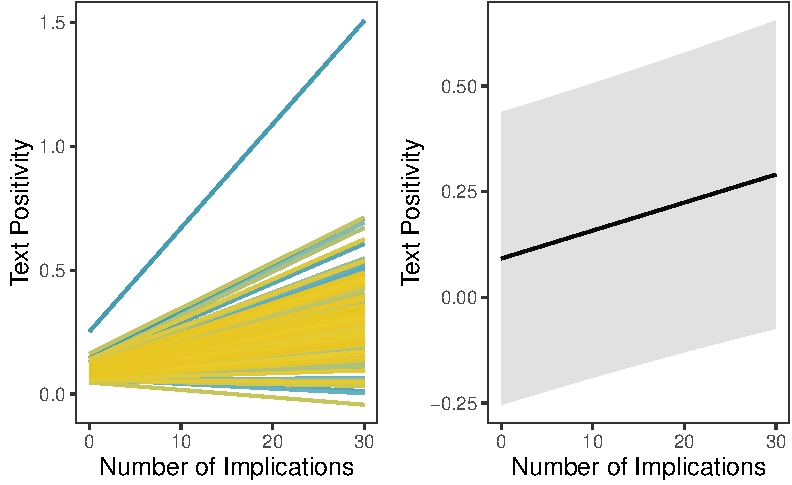
\includegraphics{EpMemNet_LabPres_htmldoc_files/figure-pdf/unnamed-chunk-13-1.pdf}

\hypertarget{strength-of-inward-causes-predicts-positivity-of-text}{%
\subsection{Strength of Inward Causes Predicts Positivity of
Text}\label{strength-of-inward-causes-predicts-positivity-of-text}}

\begin{verbatim}
boundary (singular) fit: see help('isSingular')
\end{verbatim}

\captionsetup[table]{labelformat=empty,skip=1pt}
\setlength{\LTpost}{0mm}
\begin{longtable}{lccc}
\toprule
\textbf{Characteristic} & \textbf{Beta} & \textbf{95\% CI}\textsuperscript{1} & \textbf{p-value} \\ 
\midrule
scale(strengthOut) & -0.01 & -0.06, 0.03 & 0.5 \\ 
scale(strengthIn) & 0.10 & 0.04, 0.15 & <0.001 \\ 
numID & 0.00 & -0.01, 0.00 & 0.3 \\ 
scale(length) & -0.04 & -0.08, -0.01 & 0.024 \\ 
\bottomrule
\end{longtable}
\begin{minipage}{\linewidth}
\textsuperscript{1}CI = Confidence Interval\\
\end{minipage}

\hypertarget{number-of-outward-implications-predict-certainty}{%
\subsection{Number of Outward Implications Predict
Certainty}\label{number-of-outward-implications-predict-certainty}}

\begin{verbatim}
boundary (singular) fit: see help('isSingular')
\end{verbatim}

\captionsetup[table]{labelformat=empty,skip=1pt}
\setlength{\LTpost}{0mm}
\begin{longtable}{lccc}
\toprule
\textbf{Characteristic} & \textbf{Beta} & \textbf{95\% CI}\textsuperscript{1} & \textbf{p-value} \\ 
\midrule
scale(outdegree) & 0.07 & 0.02, 0.12 & 0.010 \\ 
scale(indegree) & 0.07 & 0.03, 0.10 & <0.001 \\ 
numID & 0.00 & -0.01, 0.01 & 0.5 \\ 
scale(length) & -0.12 & -0.16, -0.09 & <0.001 \\ 
\bottomrule
\end{longtable}
\begin{minipage}{\linewidth}
\textsuperscript{1}CI = Confidence Interval\\
\end{minipage}

\begin{center}\rule{0.5\linewidth}{0.5pt}\end{center}

\begin{verbatim}
Warning: Some predictor variables are on very different scales: consider
rescaling
\end{verbatim}

\begin{verbatim}
boundary (singular) fit: see help('isSingular')
\end{verbatim}

\begin{verbatim}
Warning: Some predictor variables are on very different scales: consider
rescaling
\end{verbatim}

\begin{verbatim}
Scale for 'colour' is already present. Adding another scale for 'colour',
which will replace the existing scale.
\end{verbatim}

\begin{verbatim}
Scale for 'y' is already present. Adding another scale for 'y', which will
replace the existing scale.
\end{verbatim}

\begin{verbatim}
Warning: Removed 127 row(s) containing missing values (geom_path).
\end{verbatim}

\begin{verbatim}
Warning: Removed 127 row(s) containing missing values (geom_path).
\end{verbatim}

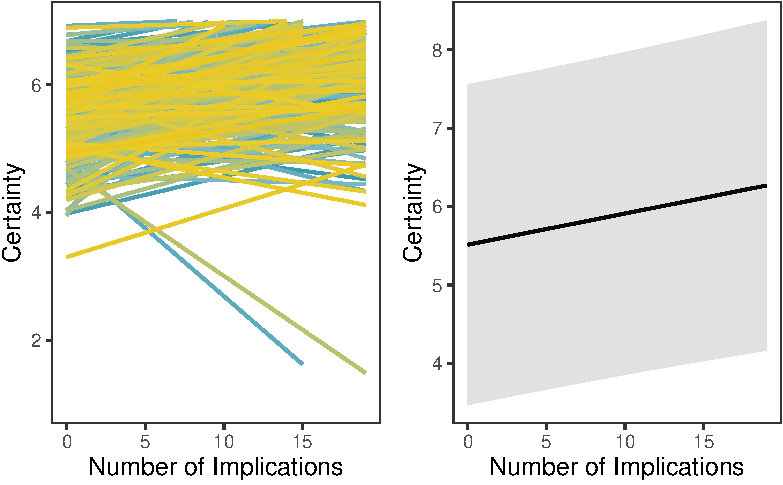
\includegraphics{EpMemNet_LabPres_htmldoc_files/figure-pdf/unnamed-chunk-16-1.pdf}

\hypertarget{strength-of-outward-implications-predicts-certainty}{%
\subsection{Strength of Outward Implications Predicts
Certainty}\label{strength-of-outward-implications-predicts-certainty}}

\begin{verbatim}
boundary (singular) fit: see help('isSingular')
\end{verbatim}

\begin{verbatim}
Warning: Model failed to converge with 1 negative eigenvalue: -9.7e-01
\end{verbatim}

\captionsetup[table]{labelformat=empty,skip=1pt}
\setlength{\LTpost}{0mm}
\begin{longtable}{lccc}
\toprule
\textbf{Characteristic} & \textbf{Beta} & \textbf{95\% CI}\textsuperscript{1} & \textbf{p-value} \\ 
\midrule
scale(strengthIn) & 0.08 & 0.05, 0.12 & <0.001 \\ 
scale(strengthOut) & 0.11 & 0.06, 0.15 & <0.001 \\ 
numID & -0.01 & -0.01, 0.00 & 0.2 \\ 
scale(length) & -0.12 & -0.16, -0.09 & <0.001 \\ 
\bottomrule
\end{longtable}
\begin{minipage}{\linewidth}
\textsuperscript{1}CI = Confidence Interval\\
\end{minipage}

\hypertarget{more-outward-implications-more-clearly-defined}{%
\subsection{More Outward Implications More Clearly
Defined}\label{more-outward-implications-more-clearly-defined}}

\captionsetup[table]{labelformat=empty,skip=1pt}
\setlength{\LTpost}{0mm}
\begin{longtable}{lccc}
\toprule
\textbf{Characteristic} & \textbf{Beta} & \textbf{95\% CI}\textsuperscript{1} & \textbf{p-value} \\ 
\midrule
scale(outdegree) & 0.06 & 0.01, 0.11 & 0.018 \\ 
scale(indegree) & 0.02 & -0.01, 0.06 & 0.2 \\ 
numID & -0.01 & -0.01, 0.00 & 0.2 \\ 
scale(length) & -0.15 & -0.19, -0.11 & <0.001 \\ 
\bottomrule
\end{longtable}
\begin{minipage}{\linewidth}
\textsuperscript{1}CI = Confidence Interval\\
\end{minipage}

\begin{center}\rule{0.5\linewidth}{0.5pt}\end{center}

\begin{verbatim}
Warning: Some predictor variables are on very different scales: consider
rescaling

Warning: Some predictor variables are on very different scales: consider
rescaling
\end{verbatim}

\begin{verbatim}
Scale for 'colour' is already present. Adding another scale for 'colour',
which will replace the existing scale.
\end{verbatim}

\begin{verbatim}
Scale for 'y' is already present. Adding another scale for 'y', which will
replace the existing scale.
\end{verbatim}

\begin{verbatim}
Warning: Removed 165 row(s) containing missing values (geom_path).
\end{verbatim}

\begin{verbatim}
Warning: Removed 165 row(s) containing missing values (geom_path).
\end{verbatim}

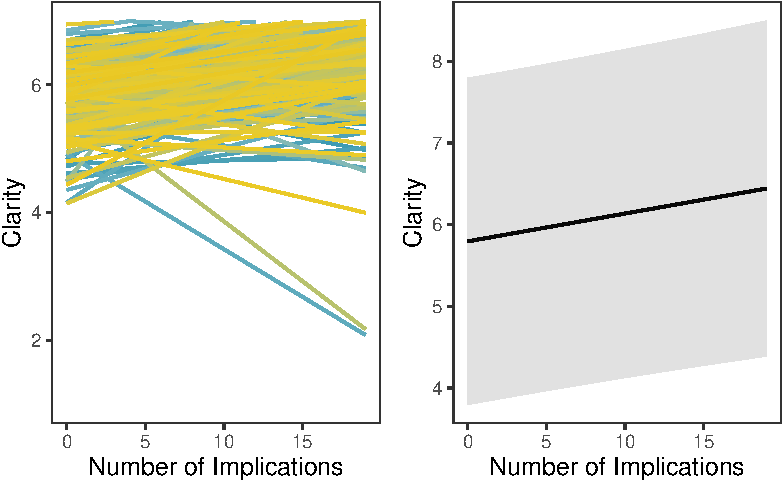
\includegraphics{EpMemNet_LabPres_htmldoc_files/figure-pdf/unnamed-chunk-19-1.pdf}

\begin{center}\rule{0.5\linewidth}{0.5pt}\end{center}

\hypertarget{moderated-by-self-concept-clarity}{%
\subsubsection{Moderated by Self-Concept
Clarity}\label{moderated-by-self-concept-clarity}}

At higher levels of self-concept clarity, outward implications matter
more for clarity of memory

\begin{verbatim}
boundary (singular) fit: see help('isSingular')
\end{verbatim}

\captionsetup[table]{labelformat=empty,skip=1pt}
\setlength{\LTpost}{0mm}
\begin{longtable}{lccc}
\toprule
\textbf{Characteristic} & \textbf{Beta} & \textbf{95\% CI}\textsuperscript{1} & \textbf{p-value} \\ 
\midrule
scale(outdegree) & -0.07 & -0.27, 0.14 & 0.5 \\ 
SCC & 0.03 & -0.07, 0.14 & 0.5 \\ 
scale(indegree) & 0.03 & -0.01, 0.06 & 0.2 \\ 
numID & 0.00 & -0.01, 0.00 & 0.3 \\ 
scale(length) & -0.15 & -0.19, -0.12 & <0.001 \\ 
scale(outdegree) * SCC & 0.04 & -0.03, 0.11 & 0.2 \\ 
\bottomrule
\end{longtable}
\begin{minipage}{\linewidth}
\textsuperscript{1}CI = Confidence Interval\\
\end{minipage}

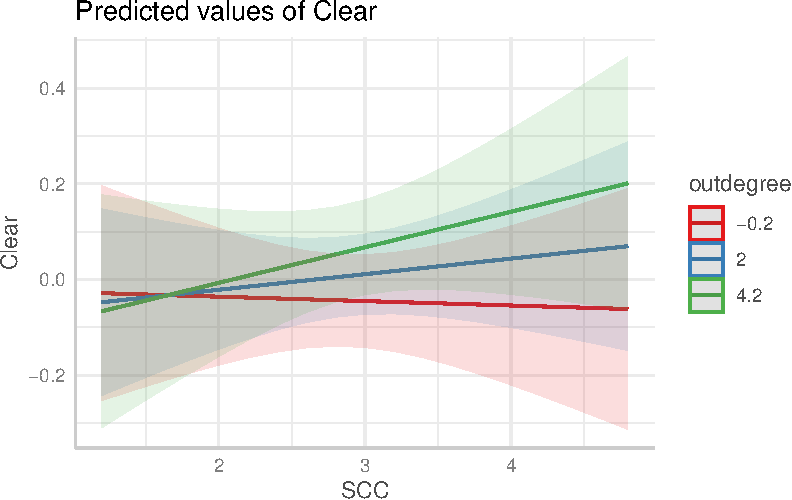
\includegraphics{EpMemNet_LabPres_htmldoc_files/figure-pdf/unnamed-chunk-20-1.pdf}

\hypertarget{stronger-outward-implications-more-clearly-defined}{%
\subsection{Stronger Outward Implications More Clearly
Defined}\label{stronger-outward-implications-more-clearly-defined}}

\begin{verbatim}
boundary (singular) fit: see help('isSingular')
\end{verbatim}

\begin{verbatim}
Warning: Model failed to converge with 1 negative eigenvalue: -1.2e+03
\end{verbatim}

\captionsetup[table]{labelformat=empty,skip=1pt}
\setlength{\LTpost}{0mm}
\begin{longtable}{lccc}
\toprule
\textbf{Characteristic} & \textbf{Beta} & \textbf{95\% CI}\textsuperscript{1} & \textbf{p-value} \\ 
\midrule
scale(strengthIn) & 0.05 & 0.01, 0.08 & 0.014 \\ 
scale(strengthOut) & 0.11 & 0.06, 0.15 & <0.001 \\ 
numID & -0.01 & -0.01, 0.00 & 0.11 \\ 
scale(length) & -0.15 & -0.18, -0.11 & <0.001 \\ 
\bottomrule
\end{longtable}
\begin{minipage}{\linewidth}
\textsuperscript{1}CI = Confidence Interval\\
\end{minipage}

\hypertarget{more-outward-implications-are-more-fundamental}{%
\subsection{More Outward Implications are More
`Fundamental'}\label{more-outward-implications-are-more-fundamental}}

\begin{verbatim}
boundary (singular) fit: see help('isSingular')
\end{verbatim}

\captionsetup[table]{labelformat=empty,skip=1pt}
\setlength{\LTpost}{0mm}
\begin{longtable}{lccc}
\toprule
\textbf{Characteristic} & \textbf{Beta} & \textbf{95\% CI}\textsuperscript{1} & \textbf{p-value} \\ 
\midrule
scale(outdegree) & 0.23 & 0.18, 0.27 & <0.001 \\ 
scale(indegree) & 0.04 & 0.01, 0.08 & 0.016 \\ 
numID & -0.01 & -0.02, 0.00 & 0.002 \\ 
scale(length) & 0.00 & -0.03, 0.04 & 0.9 \\ 
\bottomrule
\end{longtable}
\begin{minipage}{\linewidth}
\textsuperscript{1}CI = Confidence Interval\\
\end{minipage}

\begin{center}\rule{0.5\linewidth}{0.5pt}\end{center}

\begin{verbatim}
Warning: Some predictor variables are on very different scales: consider
rescaling
\end{verbatim}

\begin{verbatim}
boundary (singular) fit: see help('isSingular')
\end{verbatim}

\begin{verbatim}
Warning: Some predictor variables are on very different scales: consider
rescaling
\end{verbatim}

\begin{verbatim}
Scale for 'colour' is already present. Adding another scale for 'colour',
which will replace the existing scale.
\end{verbatim}

\begin{verbatim}
Scale for 'y' is already present. Adding another scale for 'y', which will
replace the existing scale.
\end{verbatim}

\begin{verbatim}
Warning: Removed 1021 row(s) containing missing values (geom_path).
\end{verbatim}

\begin{verbatim}
Warning: Removed 1021 row(s) containing missing values (geom_path).
\end{verbatim}

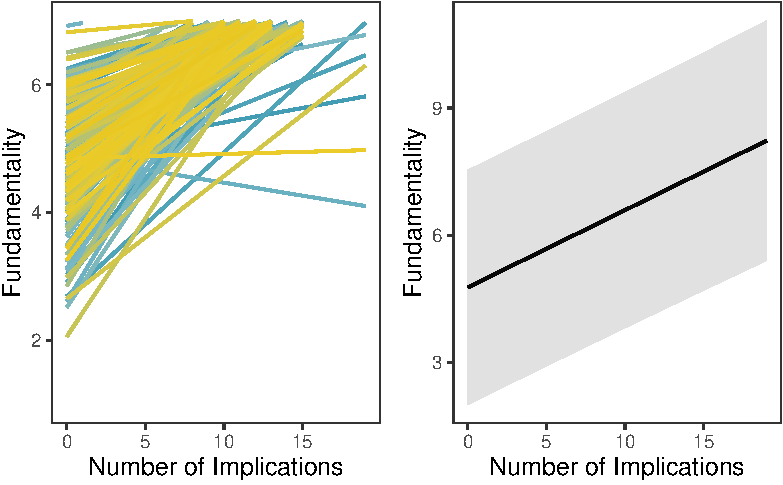
\includegraphics{EpMemNet_LabPres_htmldoc_files/figure-pdf/unnamed-chunk-23-1.pdf}

\hypertarget{stronger-outward-implicationsinward-causes-are-more-fundamental}{%
\subsection{Stronger Outward Implications/Inward Causes are More
Fundamental}\label{stronger-outward-implicationsinward-causes-are-more-fundamental}}

\begin{verbatim}
boundary (singular) fit: see help('isSingular')
\end{verbatim}

\begin{verbatim}
Warning: Model failed to converge with 1 negative eigenvalue: -2.5e+02
\end{verbatim}

\captionsetup[table]{labelformat=empty,skip=1pt}
\setlength{\LTpost}{0mm}
\begin{longtable}{lccc}
\toprule
\textbf{Characteristic} & \textbf{Beta} & \textbf{95\% CI}\textsuperscript{1} & \textbf{p-value} \\ 
\midrule
scale(strengthIn) & 0.06 & 0.02, 0.10 & 0.002 \\ 
scale(strengthOut) & 0.26 & 0.21, 0.31 & <0.001 \\ 
numID & -0.02 & -0.02, -0.01 & <0.001 \\ 
scale(length) & 0.01 & -0.02, 0.05 & 0.4 \\ 
\bottomrule
\end{longtable}
\begin{minipage}{\linewidth}
\textsuperscript{1}CI = Confidence Interval\\
\end{minipage}

\begin{center}\rule{0.5\linewidth}{0.5pt}\end{center}

\hypertarget{asymmetries-in-importance-to-self-and-others}{%
\subsection{Asymmetries in Importance to Self and
Others\ldots{}}\label{asymmetries-in-importance-to-self-and-others}}

Memories with More Causes and Implications are Perceived as More
Important to Self

\ldots{} whereas memories only with More Implications are Perceived as
More Important to Others

\hypertarget{more-outward-implications-are-perceived-as-changing-person}{%
\subsection{More Outward Implications are Perceived as Changing
Person}\label{more-outward-implications-are-perceived-as-changing-person}}

\begin{verbatim}
boundary (singular) fit: see help('isSingular')
\end{verbatim}

\captionsetup[table]{labelformat=empty,skip=1pt}
\setlength{\LTpost}{0mm}
\begin{longtable}{lccc}
\toprule
\textbf{Characteristic} & \textbf{Beta} & \textbf{95\% CI}\textsuperscript{1} & \textbf{p-value} \\ 
\midrule
scale(outdegree) & 0.21 & 0.16, 0.25 & <0.001 \\ 
scale(indegree) & 0.05 & 0.02, 0.09 & 0.003 \\ 
numID & -0.02 & -0.02, -0.01 & <0.001 \\ 
scale(length) & -0.01 & -0.04, 0.03 & 0.7 \\ 
\bottomrule
\end{longtable}
\begin{minipage}{\linewidth}
\textsuperscript{1}CI = Confidence Interval\\
\end{minipage}

\begin{center}\rule{0.5\linewidth}{0.5pt}\end{center}

\begin{verbatim}
Warning: Some predictor variables are on very different scales: consider
rescaling
\end{verbatim}

\begin{verbatim}
boundary (singular) fit: see help('isSingular')
\end{verbatim}

\begin{verbatim}
Warning: Some predictor variables are on very different scales: consider
rescaling
\end{verbatim}

\begin{verbatim}
Scale for 'colour' is already present. Adding another scale for 'colour',
which will replace the existing scale.
\end{verbatim}

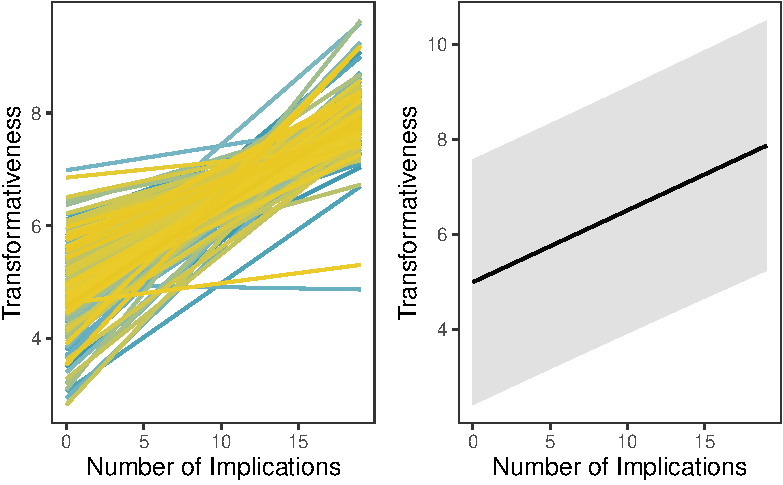
\includegraphics{EpMemNet_LabPres_htmldoc_files/figure-pdf/unnamed-chunk-26-1.pdf}

\hypertarget{stronger-outward-implications-are-perceived-as-changing-person}{%
\subsection{Stronger Outward Implications are Perceived as Changing
Person}\label{stronger-outward-implications-are-perceived-as-changing-person}}

\begin{verbatim}
boundary (singular) fit: see help('isSingular')
\end{verbatim}

\begin{verbatim}
Warning: Model failed to converge with 1 negative eigenvalue: -5.0e+00
\end{verbatim}

\captionsetup[table]{labelformat=empty,skip=1pt}
\setlength{\LTpost}{0mm}
\begin{longtable}{lccc}
\toprule
\textbf{Characteristic} & \textbf{Beta} & \textbf{95\% CI}\textsuperscript{1} & \textbf{p-value} \\ 
\midrule
scale(strengthOut) & 0.24 & 0.19, 0.28 & <0.001 \\ 
scale(strengthIn) & 0.07 & 0.03, 0.11 & <0.001 \\ 
numID & -0.02 & -0.03, -0.01 & <0.001 \\ 
scale(length) & 0.00 & -0.03, 0.04 & 0.8 \\ 
\bottomrule
\end{longtable}
\begin{minipage}{\linewidth}
\textsuperscript{1}CI = Confidence Interval\\
\end{minipage}

\begin{center}\rule{0.5\linewidth}{0.5pt}\end{center}

\hypertarget{more-outward-implications-are-more-broad}{%
\subsection{More Outward Implications are More
Broad}\label{more-outward-implications-are-more-broad}}

Supports a taxonomical/hierarchical structure?

\begin{verbatim}
boundary (singular) fit: see help('isSingular')
\end{verbatim}

\captionsetup[table]{labelformat=empty,skip=1pt}
\setlength{\LTpost}{0mm}
\begin{longtable}{lccc}
\toprule
\textbf{Characteristic} & \textbf{Beta} & \textbf{95\% CI}\textsuperscript{1} & \textbf{p-value} \\ 
\midrule
scale(outdegree) & 0.10 & 0.05, 0.15 & <0.001 \\ 
scale(indegree) & -0.01 & -0.05, 0.03 & 0.5 \\ 
numID & -0.01 & -0.02, 0.00 & 0.058 \\ 
scale(length) & 0.06 & 0.02, 0.09 & 0.003 \\ 
\bottomrule
\end{longtable}
\begin{minipage}{\linewidth}
\textsuperscript{1}CI = Confidence Interval\\
\end{minipage}

\begin{center}\rule{0.5\linewidth}{0.5pt}\end{center}

\begin{verbatim}
Warning: Some predictor variables are on very different scales: consider
rescaling
\end{verbatim}

\begin{verbatim}
Warning in checkConv(attr(opt, "derivs"), opt$par, ctrl = control$checkConv, :
Model failed to converge with max|grad| = 0.00766851 (tol = 0.002, component 1)
\end{verbatim}

\begin{verbatim}
Warning: Some predictor variables are on very different scales: consider
rescaling
\end{verbatim}

\begin{verbatim}
Scale for 'colour' is already present. Adding another scale for 'colour',
which will replace the existing scale.
\end{verbatim}

\begin{verbatim}
Scale for 'y' is already present. Adding another scale for 'y', which will
replace the existing scale.
\end{verbatim}

\begin{verbatim}
Warning: Removed 55 row(s) containing missing values (geom_path).
\end{verbatim}

\begin{verbatim}
Warning: Removed 55 row(s) containing missing values (geom_path).
\end{verbatim}

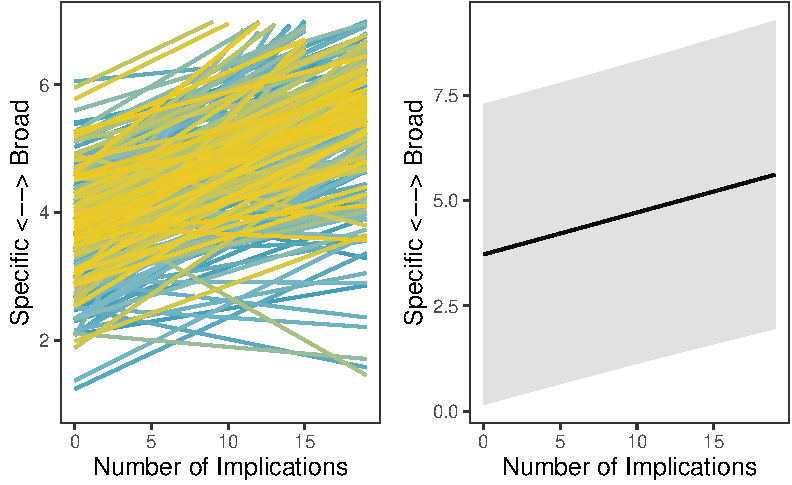
\includegraphics{EpMemNet_LabPres_htmldoc_files/figure-pdf/unnamed-chunk-29-1.pdf}

\hypertarget{stronger-outward-implications-are-more-broad}{%
\subsection{Stronger Outward Implications are More
Broad}\label{stronger-outward-implications-are-more-broad}}

\begin{verbatim}
boundary (singular) fit: see help('isSingular')
\end{verbatim}

\captionsetup[table]{labelformat=empty,skip=1pt}
\setlength{\LTpost}{0mm}
\begin{longtable}{lccc}
\toprule
\textbf{Characteristic} & \textbf{Beta} & \textbf{95\% CI}\textsuperscript{1} & \textbf{p-value} \\ 
\midrule
scale(strengthOut) & 0.10 & 0.05, 0.15 & <0.001 \\ 
scale(strengthIn) & 0.01 & -0.03, 0.05 & 0.6 \\ 
numID & -0.01 & -0.02, 0.00 & 0.059 \\ 
scale(length) & 0.07 & 0.03, 0.10 & <0.001 \\ 
\bottomrule
\end{longtable}
\begin{minipage}{\linewidth}
\textsuperscript{1}CI = Confidence Interval\\
\end{minipage}

\hypertarget{outward-implications-predicts-more-specific-neighbors}{%
\subsection{Outward Implications Predicts More Specific
Neighbors}\label{outward-implications-predicts-more-specific-neighbors}}

Further support of hierarchical structure?

\begin{verbatim}
boundary (singular) fit: see help('isSingular')
\end{verbatim}

\captionsetup[table]{labelformat=empty,skip=1pt}
\setlength{\LTpost}{0mm}
\begin{longtable}{lccc}
\toprule
\textbf{Characteristic} & \textbf{Beta} & \textbf{95\% CI}\textsuperscript{1} & \textbf{p-value} \\ 
\midrule
outdegree & -0.03 & -0.05, -0.01 & 0.001 \\ 
indegree & -0.01 & -0.02, 0.01 & 0.4 \\ 
numID & -0.01 & -0.02, 0.00 & 0.2 \\ 
scale(length) & 0.04 & 0.00, 0.07 & 0.030 \\ 
\bottomrule
\end{longtable}
\begin{minipage}{\linewidth}
\textsuperscript{1}CI = Confidence Interval\\
\end{minipage}

\hypertarget{more-outward-implications-are-more-distinct}{%
\subsection{More Outward Implications are More
Distinct}\label{more-outward-implications-are-more-distinct}}

\begin{verbatim}
boundary (singular) fit: see help('isSingular')
\end{verbatim}

\captionsetup[table]{labelformat=empty,skip=1pt}
\setlength{\LTpost}{0mm}
\begin{longtable}{lccc}
\toprule
\textbf{Characteristic} & \textbf{Beta} & \textbf{95\% CI}\textsuperscript{1} & \textbf{p-value} \\ 
\midrule
scale(outdegree) & 0.09 & 0.04, 0.13 & <0.001 \\ 
scale(indegree) & 0.02 & -0.02, 0.05 & 0.3 \\ 
numID & -0.01 & -0.02, 0.00 & 0.12 \\ 
scale(length) & -0.04 & -0.07, 0.00 & 0.042 \\ 
\bottomrule
\end{longtable}
\begin{minipage}{\linewidth}
\textsuperscript{1}CI = Confidence Interval\\
\end{minipage}

\begin{center}\rule{0.5\linewidth}{0.5pt}\end{center}

\begin{verbatim}
Warning: Some predictor variables are on very different scales: consider
rescaling
\end{verbatim}

\begin{verbatim}
boundary (singular) fit: see help('isSingular')
\end{verbatim}

\begin{verbatim}
Warning: Some predictor variables are on very different scales: consider
rescaling
\end{verbatim}

\begin{verbatim}
Scale for 'colour' is already present. Adding another scale for 'colour',
which will replace the existing scale.
\end{verbatim}

\begin{verbatim}
Scale for 'y' is already present. Adding another scale for 'y', which will
replace the existing scale.
\end{verbatim}

\begin{verbatim}
Warning: Removed 51 row(s) containing missing values (geom_path).
\end{verbatim}

\begin{verbatim}
Warning: Removed 51 row(s) containing missing values (geom_path).
\end{verbatim}

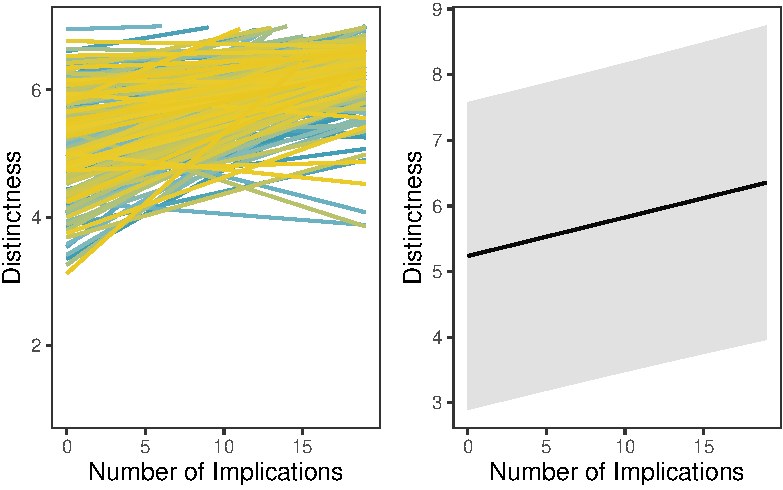
\includegraphics{EpMemNet_LabPres_htmldoc_files/figure-pdf/unnamed-chunk-33-1.pdf}

\hypertarget{stronger-outward-implications-are-more-distinct}{%
\subsection{Stronger Outward Implications are More
Distinct}\label{stronger-outward-implications-are-more-distinct}}

\captionsetup[table]{labelformat=empty,skip=1pt}
\setlength{\LTpost}{0mm}
\begin{longtable}{lccc}
\toprule
\textbf{Characteristic} & \textbf{Beta} & \textbf{95\% CI}\textsuperscript{1} & \textbf{p-value} \\ 
\midrule
scale(strengthOut) & 0.12 & 0.07, 0.17 & <0.001 \\ 
scale(strengthIn) & 0.01 & -0.04, 0.05 & 0.8 \\ 
numID & -0.01 & -0.02, 0.00 & 0.053 \\ 
scale(length) & -0.04 & -0.07, 0.00 & 0.051 \\ 
\bottomrule
\end{longtable}
\begin{minipage}{\linewidth}
\textsuperscript{1}CI = Confidence Interval\\
\end{minipage}

\hypertarget{similarities}{%
\section{Similarities}\label{similarities}}

Memories that share other memories in common (as implications or causes)
are reflected upon similarly\ldots{}

\hypertarget{relational-similarity-predicts-similarity-in-positivity}{%
\subsection{Relational Similarity Predicts Similarity in
Positivity}\label{relational-similarity-predicts-similarity-in-positivity}}

\captionsetup[table]{labelformat=empty,skip=1pt}
\setlength{\LTpost}{0mm}
\begin{longtable}{lccc}
\toprule
\textbf{Characteristic} & \textbf{Beta} & \textbf{95\% CI}\textsuperscript{1} & \textbf{p-value} \\ 
\midrule
scale(Sim) & -0.04 & -0.07, -0.02 & <0.001 \\ 
\bottomrule
\end{longtable}
\begin{minipage}{\linewidth}
\textsuperscript{1}CI = Confidence Interval\\
\end{minipage}

\hypertarget{relational-similarity-predicts-similarity-in-negativity}{%
\subsection{Relational Similarity Predicts Similarity in
Negativity}\label{relational-similarity-predicts-similarity-in-negativity}}

\captionsetup[table]{labelformat=empty,skip=1pt}
\setlength{\LTpost}{0mm}
\begin{longtable}{lccc}
\toprule
\textbf{Characteristic} & \textbf{Beta} & \textbf{95\% CI}\textsuperscript{1} & \textbf{p-value} \\ 
\midrule
scale(Sim) & -0.08 & -0.10, -0.05 & <0.001 \\ 
\bottomrule
\end{longtable}
\begin{minipage}{\linewidth}
\textsuperscript{1}CI = Confidence Interval\\
\end{minipage}

\hypertarget{relational-similarity-predicts-similarity-in-changeability}{%
\subsection{Relational Similarity Predicts Similarity in
Changeability}\label{relational-similarity-predicts-similarity-in-changeability}}

\captionsetup[table]{labelformat=empty,skip=1pt}
\setlength{\LTpost}{0mm}
\begin{longtable}{lccc}
\toprule
\textbf{Characteristic} & \textbf{Beta} & \textbf{95\% CI}\textsuperscript{1} & \textbf{p-value} \\ 
\midrule
scale(Sim) & -0.04 & -0.06, -0.02 & 0.001 \\ 
\bottomrule
\end{longtable}
\begin{minipage}{\linewidth}
\textsuperscript{1}CI = Confidence Interval\\
\end{minipage}

\hypertarget{relational-similarity-predicts-similarity-in-clarity}{%
\subsection{Relational Similarity Predicts Similarity in
Clarity}\label{relational-similarity-predicts-similarity-in-clarity}}

\captionsetup[table]{labelformat=empty,skip=1pt}
\setlength{\LTpost}{0mm}
\begin{longtable}{lccc}
\toprule
\textbf{Characteristic} & \textbf{Beta} & \textbf{95\% CI}\textsuperscript{1} & \textbf{p-value} \\ 
\midrule
scale(Sim) & -0.04 & -0.06, -0.02 & 0.001 \\ 
\bottomrule
\end{longtable}
\begin{minipage}{\linewidth}
\textsuperscript{1}CI = Confidence Interval\\
\end{minipage}

\hypertarget{relational-similarity-predicts-similarity-in-certainty}{%
\subsection{Relational Similarity Predicts Similarity in
Certainty}\label{relational-similarity-predicts-similarity-in-certainty}}

\captionsetup[table]{labelformat=empty,skip=1pt}
\setlength{\LTpost}{0mm}
\begin{longtable}{lccc}
\toprule
\textbf{Characteristic} & \textbf{Beta} & \textbf{95\% CI}\textsuperscript{1} & \textbf{p-value} \\ 
\midrule
scale(Sim) & -0.04 & -0.07, -0.02 & <0.001 \\ 
\bottomrule
\end{longtable}
\begin{minipage}{\linewidth}
\textsuperscript{1}CI = Confidence Interval\\
\end{minipage}

\hypertarget{relational-similarity-predicts-similarity-in-breadth}{%
\subsection{Relational Similarity Predicts Similarity in
Breadth}\label{relational-similarity-predicts-similarity-in-breadth}}

\captionsetup[table]{labelformat=empty,skip=1pt}
\setlength{\LTpost}{0mm}
\begin{longtable}{lccc}
\toprule
\textbf{Characteristic} & \textbf{Beta} & \textbf{95\% CI}\textsuperscript{1} & \textbf{p-value} \\ 
\midrule
scale(Sim) & -0.05 & -0.07, -0.03 & <0.001 \\ 
\bottomrule
\end{longtable}
\begin{minipage}{\linewidth}
\textsuperscript{1}CI = Confidence Interval\\
\end{minipage}

\hypertarget{individual-differences-main-effects}{%
\section{Individual Differences Main
Effects}\label{individual-differences-main-effects}}

\hypertarget{self-esteem}{%
\subsection{Self-Esteem}\label{self-esteem}}

\begin{center}\rule{0.5\linewidth}{0.5pt}\end{center}

\hypertarget{no-effect-on-outdegree}{%
\subsubsection{No Effect on Outdegree}\label{no-effect-on-outdegree}}

\begin{verbatim}
boundary (singular) fit: see help('isSingular')
\end{verbatim}

\captionsetup[table]{labelformat=empty,skip=1pt}
\setlength{\LTpost}{0mm}
\begin{longtable}{lccc}
\toprule
\textbf{Characteristic} & \textbf{log(IRR)}\textsuperscript{1} & \textbf{95\% CI}\textsuperscript{1} & \textbf{p-value} \\ 
\midrule
scale(SE) & -0.04 & -0.11, 0.03 & 0.3 \\ 
numID & 0.03 & 0.02, 0.04 & <0.001 \\ 
scale(length) & 0.09 & 0.06, 0.11 & <0.001 \\ 
\bottomrule
\end{longtable}
\begin{minipage}{\linewidth}
\textsuperscript{1}IRR = Incidence Rate Ratio, CI = Confidence Interval\\
\end{minipage}

\begin{center}\rule{0.5\linewidth}{0.5pt}\end{center}

\hypertarget{no-effect-on-indegree}{%
\subsubsection{No Effect on Indegree}\label{no-effect-on-indegree}}

\begin{verbatim}
boundary (singular) fit: see help('isSingular')
\end{verbatim}

\captionsetup[table]{labelformat=empty,skip=1pt}
\setlength{\LTpost}{0mm}
\begin{longtable}{lccc}
\toprule
\textbf{Characteristic} & \textbf{log(IRR)}\textsuperscript{1} & \textbf{95\% CI}\textsuperscript{1} & \textbf{p-value} \\ 
\midrule
scale(SE) & -0.06 & -0.13, 0.01 & 0.10 \\ 
numID & 0.02 & 0.01, 0.03 & <0.001 \\ 
scale(length) & -0.22 & -0.25, -0.18 & <0.001 \\ 
\bottomrule
\end{longtable}
\begin{minipage}{\linewidth}
\textsuperscript{1}IRR = Incidence Rate Ratio, CI = Confidence Interval\\
\end{minipage}

\begin{center}\rule{0.5\linewidth}{0.5pt}\end{center}

\hypertarget{small-effect-of-self-esteem-on-strength}{%
\subsubsection{Small Effect of Self-Esteem on
Strength}\label{small-effect-of-self-esteem-on-strength}}

More self-esteem, less similarity among memories

\captionsetup[table]{labelformat=empty,skip=1pt}
\setlength{\LTpost}{0mm}
\begin{longtable}{lccc}
\toprule
\textbf{Characteristic} & \textbf{Beta} & \textbf{95\% CI}\textsuperscript{1} & \textbf{p-value} \\ 
\midrule
scale(SE) & -0.10 & -0.17, -0.03 & 0.008 \\ 
numID & 0.03 & 0.02, 0.04 & <0.001 \\ 
scale(length) & -0.09 & -0.13, -0.06 & <0.001 \\ 
\bottomrule
\end{longtable}
\begin{minipage}{\linewidth}
\textsuperscript{1}CI = Confidence Interval\\
\end{minipage}

\hypertarget{self-concept-clarity}{%
\subsection{Self-Concept Clarity}\label{self-concept-clarity}}

\begin{center}\rule{0.5\linewidth}{0.5pt}\end{center}

\hypertarget{no-effect-on-outdegree-1}{%
\subsubsection{No Effect on Outdegree}\label{no-effect-on-outdegree-1}}

\captionsetup[table]{labelformat=empty,skip=1pt}
\setlength{\LTpost}{0mm}
\begin{longtable}{lccc}
\toprule
\textbf{Characteristic} & \textbf{log(IRR)}\textsuperscript{1} & \textbf{95\% CI}\textsuperscript{1} & \textbf{p-value} \\ 
\midrule
scale(SCC) & 0.06 & -0.01, 0.13 & 0.095 \\ 
numID & 0.03 & 0.02, 0.04 & <0.001 \\ 
scale(length) & 0.09 & 0.06, 0.11 & <0.001 \\ 
\bottomrule
\end{longtable}
\begin{minipage}{\linewidth}
\textsuperscript{1}IRR = Incidence Rate Ratio, CI = Confidence Interval\\
\end{minipage}

\begin{center}\rule{0.5\linewidth}{0.5pt}\end{center}

\hypertarget{no-effect-on-indegree-1}{%
\subsubsection{No Effect on Indegree}\label{no-effect-on-indegree-1}}

\captionsetup[table]{labelformat=empty,skip=1pt}
\setlength{\LTpost}{0mm}
\begin{longtable}{lccc}
\toprule
\textbf{Characteristic} & \textbf{log(IRR)}\textsuperscript{1} & \textbf{95\% CI}\textsuperscript{1} & \textbf{p-value} \\ 
\midrule
scale(SCC) & 0.10 & 0.03, 0.16 & 0.005 \\ 
numID & 0.02 & 0.02, 0.03 & <0.001 \\ 
scale(length) & -0.21 & -0.24, -0.18 & <0.001 \\ 
\bottomrule
\end{longtable}
\begin{minipage}{\linewidth}
\textsuperscript{1}IRR = Incidence Rate Ratio, CI = Confidence Interval\\
\end{minipage}

\begin{center}\rule{0.5\linewidth}{0.5pt}\end{center}

\hypertarget{no-effect-on-strength}{%
\subsubsection{No Effect on Strength}\label{no-effect-on-strength}}

\captionsetup[table]{labelformat=empty,skip=1pt}
\setlength{\LTpost}{0mm}
\begin{longtable}{lccc}
\toprule
\textbf{Characteristic} & \textbf{Beta} & \textbf{95\% CI}\textsuperscript{1} & \textbf{p-value} \\ 
\midrule
scale(SCC) & 0.08 & 0.01, 0.15 & 0.032 \\ 
numID & 0.03 & 0.02, 0.04 & <0.001 \\ 
scale(length) & -0.09 & -0.13, -0.06 & <0.001 \\ 
\bottomrule
\end{longtable}
\begin{minipage}{\linewidth}
\textsuperscript{1}CI = Confidence Interval\\
\end{minipage}

\hypertarget{depression}{%
\subsection{Depression}\label{depression}}

\begin{center}\rule{0.5\linewidth}{0.5pt}\end{center}

\hypertarget{no-effect-on-outdegree-2}{%
\subsubsection{No Effect on Outdegree}\label{no-effect-on-outdegree-2}}

\captionsetup[table]{labelformat=empty,skip=1pt}
\setlength{\LTpost}{0mm}
\begin{longtable}{lccc}
\toprule
\textbf{Characteristic} & \textbf{log(IRR)}\textsuperscript{1} & \textbf{95\% CI}\textsuperscript{1} & \textbf{p-value} \\ 
\midrule
scale(CESD) & 0.02 & -0.05, 0.09 & 0.6 \\ 
numID & 0.03 & 0.02, 0.04 & <0.001 \\ 
scale(length) & 0.09 & 0.06, 0.12 & <0.001 \\ 
\bottomrule
\end{longtable}
\begin{minipage}{\linewidth}
\textsuperscript{1}IRR = Incidence Rate Ratio, CI = Confidence Interval\\
\end{minipage}

\begin{center}\rule{0.5\linewidth}{0.5pt}\end{center}

\hypertarget{no-effect-on-indegree-2}{%
\subsubsection{No Effect on Indegree}\label{no-effect-on-indegree-2}}

\captionsetup[table]{labelformat=empty,skip=1pt}
\setlength{\LTpost}{0mm}
\begin{longtable}{lccc}
\toprule
\textbf{Characteristic} & \textbf{log(IRR)}\textsuperscript{1} & \textbf{95\% CI}\textsuperscript{1} & \textbf{p-value} \\ 
\midrule
scale(CESD) & 0.00 & -0.07, 0.07 & >0.9 \\ 
numID & 0.02 & 0.02, 0.03 & <0.001 \\ 
scale(length) & -0.21 & -0.25, -0.18 & <0.001 \\ 
\bottomrule
\end{longtable}
\begin{minipage}{\linewidth}
\textsuperscript{1}IRR = Incidence Rate Ratio, CI = Confidence Interval\\
\end{minipage}

\begin{center}\rule{0.5\linewidth}{0.5pt}\end{center}

\hypertarget{no-effect-on-strength-1}{%
\subsubsection{No Effect on Strength}\label{no-effect-on-strength-1}}

\captionsetup[table]{labelformat=empty,skip=1pt}
\setlength{\LTpost}{0mm}
\begin{longtable}{lccc}
\toprule
\textbf{Characteristic} & \textbf{Beta} & \textbf{95\% CI}\textsuperscript{1} & \textbf{p-value} \\ 
\midrule
scale(CESD) & -0.01 & -0.08, 0.06 & 0.8 \\ 
numID & 0.03 & 0.02, 0.04 & <0.001 \\ 
scale(length) & -0.09 & -0.13, -0.06 & <0.001 \\ 
\bottomrule
\end{longtable}
\begin{minipage}{\linewidth}
\textsuperscript{1}CI = Confidence Interval\\
\end{minipage}

\hypertarget{need-for-cognition}{%
\subsection{Need for Cognition}\label{need-for-cognition}}

\begin{center}\rule{0.5\linewidth}{0.5pt}\end{center}

\hypertarget{no-effect-on-outdegree-3}{%
\subsubsection{No Effect on Outdegree}\label{no-effect-on-outdegree-3}}

\captionsetup[table]{labelformat=empty,skip=1pt}
\setlength{\LTpost}{0mm}
\begin{longtable}{lccc}
\toprule
\textbf{Characteristic} & \textbf{log(IRR)}\textsuperscript{1} & \textbf{95\% CI}\textsuperscript{1} & \textbf{p-value} \\ 
\midrule
scale(NFC) & 0.06 & -0.01, 0.13 & 0.11 \\ 
numID & 0.03 & 0.02, 0.04 & <0.001 \\ 
scale(length) & 0.09 & 0.06, 0.11 & <0.001 \\ 
\bottomrule
\end{longtable}
\begin{minipage}{\linewidth}
\textsuperscript{1}IRR = Incidence Rate Ratio, CI = Confidence Interval\\
\end{minipage}

\begin{center}\rule{0.5\linewidth}{0.5pt}\end{center}

\hypertarget{more-need-for-cognition-more-inward-causes}{%
\subsubsection{More need for cognition, more inward
causes}\label{more-need-for-cognition-more-inward-causes}}

\begin{verbatim}
Warning in checkConv(attr(opt, "derivs"), opt$par, ctrl = control$checkConv, :
Model failed to converge with max|grad| = 0.00203105 (tol = 0.002, component 1)
\end{verbatim}

\captionsetup[table]{labelformat=empty,skip=1pt}
\setlength{\LTpost}{0mm}
\begin{longtable}{lccc}
\toprule
\textbf{Characteristic} & \textbf{log(IRR)}\textsuperscript{1} & \textbf{95\% CI}\textsuperscript{1} & \textbf{p-value} \\ 
\midrule
scale(NFC) & 0.09 & 0.02, 0.15 & 0.013 \\ 
numID & 0.02 & 0.02, 0.03 & <0.001 \\ 
scale(length) & -0.21 & -0.24, -0.18 & <0.001 \\ 
\bottomrule
\end{longtable}
\begin{minipage}{\linewidth}
\textsuperscript{1}IRR = Incidence Rate Ratio, CI = Confidence Interval\\
\end{minipage}

\begin{center}\rule{0.5\linewidth}{0.5pt}\end{center}

\hypertarget{more-need-for-cognition-more-similarity-to-other-memories}{%
\subsubsection{More need for cognition, more similarity to other
memories}\label{more-need-for-cognition-more-similarity-to-other-memories}}

\captionsetup[table]{labelformat=empty,skip=1pt}
\setlength{\LTpost}{0mm}
\begin{longtable}{lccc}
\toprule
\textbf{Characteristic} & \textbf{Beta} & \textbf{95\% CI}\textsuperscript{1} & \textbf{p-value} \\ 
\midrule
scale(NFC) & 0.09 & 0.01, 0.16 & 0.018 \\ 
numID & 0.03 & 0.02, 0.04 & <0.001 \\ 
scale(length) & -0.09 & -0.13, -0.06 & <0.001 \\ 
\bottomrule
\end{longtable}
\begin{minipage}{\linewidth}
\textsuperscript{1}CI = Confidence Interval\\
\end{minipage}

\hypertarget{no-effects-of-self-ambivalence}{%
\subsection{No Effects of
Self-Ambivalence}\label{no-effects-of-self-ambivalence}}

\begin{center}\rule{0.5\linewidth}{0.5pt}\end{center}

\hypertarget{no-effect-on-outdegree-4}{%
\subsubsection{No effect on outdegree}\label{no-effect-on-outdegree-4}}

\captionsetup[table]{labelformat=empty,skip=1pt}
\setlength{\LTpost}{0mm}
\begin{longtable}{lccc}
\toprule
\textbf{Characteristic} & \textbf{log(IRR)}\textsuperscript{1} & \textbf{95\% CI}\textsuperscript{1} & \textbf{p-value} \\ 
\midrule
scale(SAM) & 0.03 & -0.03, 0.10 & 0.3 \\ 
numID & 0.03 & 0.02, 0.04 & <0.001 \\ 
scale(length) & 0.09 & 0.06, 0.11 & <0.001 \\ 
\bottomrule
\end{longtable}
\begin{minipage}{\linewidth}
\textsuperscript{1}IRR = Incidence Rate Ratio, CI = Confidence Interval\\
\end{minipage}

\begin{center}\rule{0.5\linewidth}{0.5pt}\end{center}

\hypertarget{no-effect-on-indegree-3}{%
\subsubsection{No effect on indegree}\label{no-effect-on-indegree-3}}

\captionsetup[table]{labelformat=empty,skip=1pt}
\setlength{\LTpost}{0mm}
\begin{longtable}{lccc}
\toprule
\textbf{Characteristic} & \textbf{log(IRR)}\textsuperscript{1} & \textbf{95\% CI}\textsuperscript{1} & \textbf{p-value} \\ 
\midrule
scale(SAM) & 0.01 & -0.06, 0.08 & 0.8 \\ 
numID & 0.02 & 0.02, 0.03 & <0.001 \\ 
scale(length) & -0.21 & -0.24, -0.18 & <0.001 \\ 
\bottomrule
\end{longtable}
\begin{minipage}{\linewidth}
\textsuperscript{1}IRR = Incidence Rate Ratio, CI = Confidence Interval\\
\end{minipage}

\begin{center}\rule{0.5\linewidth}{0.5pt}\end{center}

\hypertarget{no-effect-on-strength-2}{%
\subsubsection{No effect on strength}\label{no-effect-on-strength-2}}

\captionsetup[table]{labelformat=empty,skip=1pt}
\setlength{\LTpost}{0mm}
\begin{longtable}{lccc}
\toprule
\textbf{Characteristic} & \textbf{Beta} & \textbf{95\% CI}\textsuperscript{1} & \textbf{p-value} \\ 
\midrule
scale(SAM) & 0.01 & -0.06, 0.08 & 0.8 \\ 
numID & 0.03 & 0.02, 0.04 & <0.001 \\ 
scale(length) & -0.09 & -0.12, -0.06 & <0.001 \\ 
\bottomrule
\end{longtable}
\begin{minipage}{\linewidth}
\textsuperscript{1}CI = Confidence Interval\\
\end{minipage}

\hypertarget{small-effect-of-sense-of-self-on-inward-causes}{%
\subsection{Small Effect of Sense of Self on Inward
Causes}\label{small-effect-of-sense-of-self-on-inward-causes}}

\begin{center}\rule{0.5\linewidth}{0.5pt}\end{center}

\hypertarget{no-effect-on-outdegree-5}{%
\subsubsection{No effect on outdegree}\label{no-effect-on-outdegree-5}}

\captionsetup[table]{labelformat=empty,skip=1pt}
\setlength{\LTpost}{0mm}
\begin{longtable}{lccc}
\toprule
\textbf{Characteristic} & \textbf{log(IRR)}\textsuperscript{1} & \textbf{95\% CI}\textsuperscript{1} & \textbf{p-value} \\ 
\midrule
scale(SOS) & -0.02 & -0.09, 0.05 & 0.6 \\ 
numID & 0.03 & 0.02, 0.04 & <0.001 \\ 
scale(length) & 0.09 & 0.06, 0.11 & <0.001 \\ 
\bottomrule
\end{longtable}
\begin{minipage}{\linewidth}
\textsuperscript{1}IRR = Incidence Rate Ratio, CI = Confidence Interval\\
\end{minipage}

\begin{center}\rule{0.5\linewidth}{0.5pt}\end{center}

\hypertarget{lower-sense-of-self-more-inward-causes}{%
\subsection{Lower sense of self, more inward
causes}\label{lower-sense-of-self-more-inward-causes}}

\captionsetup[table]{labelformat=empty,skip=1pt}
\setlength{\LTpost}{0mm}
\begin{longtable}{lccc}
\toprule
\textbf{Characteristic} & \textbf{log(IRR)}\textsuperscript{1} & \textbf{95\% CI}\textsuperscript{1} & \textbf{p-value} \\ 
\midrule
scale(SOS) & -0.06 & -0.13, 0.01 & 0.087 \\ 
numID & 0.02 & 0.02, 0.03 & <0.001 \\ 
scale(length) & -0.21 & -0.25, -0.18 & <0.001 \\ 
\bottomrule
\end{longtable}
\begin{minipage}{\linewidth}
\textsuperscript{1}IRR = Incidence Rate Ratio, CI = Confidence Interval\\
\end{minipage}

\begin{center}\rule{0.5\linewidth}{0.5pt}\end{center}

\hypertarget{lower-sense-of-self-more-similarity-to-other-memories}{%
\subsubsection{Lower sense of self, more similarity to other
memories}\label{lower-sense-of-self-more-similarity-to-other-memories}}

\captionsetup[table]{labelformat=empty,skip=1pt}
\setlength{\LTpost}{0mm}
\begin{longtable}{lccc}
\toprule
\textbf{Characteristic} & \textbf{Beta} & \textbf{95\% CI}\textsuperscript{1} & \textbf{p-value} \\ 
\midrule
scale(SOS) & -0.07 & -0.15, 0.01 & 0.077 \\ 
numID & 0.03 & 0.02, 0.04 & <0.001 \\ 
scale(length) & -0.09 & -0.13, -0.06 & <0.001 \\ 
\bottomrule
\end{longtable}
\begin{minipage}{\linewidth}
\textsuperscript{1}CI = Confidence Interval\\
\end{minipage}

\hypertarget{small-effect-of-psychopathy-on-outward-implications}{%
\subsection{Small Effect of Psychopathy on Outward
Implications}\label{small-effect-of-psychopathy-on-outward-implications}}

\begin{center}\rule{0.5\linewidth}{0.5pt}\end{center}

\hypertarget{lower-psychopathy-more-outward-implications}{%
\subsection{Lower psychopathy, more outward
implications}\label{lower-psychopathy-more-outward-implications}}

\captionsetup[table]{labelformat=empty,skip=1pt}
\setlength{\LTpost}{0mm}
\begin{longtable}{lccc}
\toprule
\textbf{Characteristic} & \textbf{log(IRR)}\textsuperscript{1} & \textbf{95\% CI}\textsuperscript{1} & \textbf{p-value} \\ 
\midrule
scale(DT\_P) & -0.05 & -0.12, 0.02 & 0.2 \\ 
numID & 0.03 & 0.02, 0.04 & <0.001 \\ 
scale(length) & 0.09 & 0.06, 0.12 & <0.001 \\ 
\bottomrule
\end{longtable}
\begin{minipage}{\linewidth}
\textsuperscript{1}IRR = Incidence Rate Ratio, CI = Confidence Interval\\
\end{minipage}

\begin{center}\rule{0.5\linewidth}{0.5pt}\end{center}

\hypertarget{no-effect-on-indegree-4}{%
\subsubsection{No effect on indegree}\label{no-effect-on-indegree-4}}

\captionsetup[table]{labelformat=empty,skip=1pt}
\setlength{\LTpost}{0mm}
\begin{longtable}{lccc}
\toprule
\textbf{Characteristic} & \textbf{log(IRR)}\textsuperscript{1} & \textbf{95\% CI}\textsuperscript{1} & \textbf{p-value} \\ 
\midrule
scale(DT\_P) & -0.06 & -0.14, 0.01 & 0.10 \\ 
numID & 0.02 & 0.02, 0.03 & <0.001 \\ 
scale(length) & -0.21 & -0.25, -0.18 & <0.001 \\ 
\bottomrule
\end{longtable}
\begin{minipage}{\linewidth}
\textsuperscript{1}IRR = Incidence Rate Ratio, CI = Confidence Interval\\
\end{minipage}

\begin{center}\rule{0.5\linewidth}{0.5pt}\end{center}

\hypertarget{no-effect-on-strength-3}{%
\subsubsection{No effect on strength}\label{no-effect-on-strength-3}}

\captionsetup[table]{labelformat=empty,skip=1pt}
\setlength{\LTpost}{0mm}
\begin{longtable}{lccc}
\toprule
\textbf{Characteristic} & \textbf{Beta} & \textbf{95\% CI}\textsuperscript{1} & \textbf{p-value} \\ 
\midrule
scale(DT\_P) & -0.05 & -0.13, 0.03 & 0.2 \\ 
numID & 0.03 & 0.02, 0.04 & <0.001 \\ 
scale(length) & -0.09 & -0.13, -0.06 & <0.001 \\ 
\bottomrule
\end{longtable}
\begin{minipage}{\linewidth}
\textsuperscript{1}CI = Confidence Interval\\
\end{minipage}

\hypertarget{small-effects-of-dialectical-self}{%
\subsection{Small Effects of Dialectical
Self}\label{small-effects-of-dialectical-self}}

\begin{center}\rule{0.5\linewidth}{0.5pt}\end{center}

\hypertarget{no-effect-of-outdegree}{%
\subsubsection{No effect of outdegree}\label{no-effect-of-outdegree}}

\captionsetup[table]{labelformat=empty,skip=1pt}
\setlength{\LTpost}{0mm}
\begin{longtable}{lccc}
\toprule
\textbf{Characteristic} & \textbf{log(IRR)}\textsuperscript{1} & \textbf{95\% CI}\textsuperscript{1} & \textbf{p-value} \\ 
\midrule
scale(DS) & -0.06 & -0.13, 0.01 & 0.091 \\ 
numID & 0.03 & 0.02, 0.04 & <0.001 \\ 
scale(length) & 0.09 & 0.06, 0.11 & <0.001 \\ 
\bottomrule
\end{longtable}
\begin{minipage}{\linewidth}
\textsuperscript{1}IRR = Incidence Rate Ratio, CI = Confidence Interval\\
\end{minipage}

\begin{center}\rule{0.5\linewidth}{0.5pt}\end{center}

\hypertarget{lower-dialectical-self-views-more-inward-causes}{%
\subsubsection{Lower dialectical self-views, more inward
causes}\label{lower-dialectical-self-views-more-inward-causes}}

\captionsetup[table]{labelformat=empty,skip=1pt}
\setlength{\LTpost}{0mm}
\begin{longtable}{lccc}
\toprule
\textbf{Characteristic} & \textbf{log(IRR)}\textsuperscript{1} & \textbf{95\% CI}\textsuperscript{1} & \textbf{p-value} \\ 
\midrule
scale(DS) & -0.08 & -0.15, -0.01 & 0.019 \\ 
numID & 0.02 & 0.02, 0.03 & <0.001 \\ 
scale(length) & -0.21 & -0.25, -0.18 & <0.001 \\ 
\bottomrule
\end{longtable}
\begin{minipage}{\linewidth}
\textsuperscript{1}IRR = Incidence Rate Ratio, CI = Confidence Interval\\
\end{minipage}

\begin{center}\rule{0.5\linewidth}{0.5pt}\end{center}

\hypertarget{more-dialectical-self-views-less-similarity-to-other-memories}{%
\subsubsection{More dialectical self-views, less similarity to other
memories}\label{more-dialectical-self-views-less-similarity-to-other-memories}}

\captionsetup[table]{labelformat=empty,skip=1pt}
\setlength{\LTpost}{0mm}
\begin{longtable}{lccc}
\toprule
\textbf{Characteristic} & \textbf{Beta} & \textbf{95\% CI}\textsuperscript{1} & \textbf{p-value} \\ 
\midrule
scale(DS) & -0.10 & -0.18, -0.03 & 0.005 \\ 
numID & 0.03 & 0.02, 0.04 & <0.001 \\ 
scale(length) & -0.09 & -0.13, -0.06 & <0.001 \\ 
\bottomrule
\end{longtable}
\begin{minipage}{\linewidth}
\textsuperscript{1}CI = Confidence Interval\\
\end{minipage}

\hypertarget{small-effect-of-interoceptive-awareness}{%
\subsection{Small Effect of Interoceptive
Awareness}\label{small-effect-of-interoceptive-awareness}}

\begin{center}\rule{0.5\linewidth}{0.5pt}\end{center}

\hypertarget{no-effect-on-outdegree-6}{%
\subsubsection{No effect on outdegree}\label{no-effect-on-outdegree-6}}

\begin{verbatim}
Warning in checkConv(attr(opt, "derivs"), opt$par, ctrl = control$checkConv, :
Model failed to converge with max|grad| = 0.00351421 (tol = 0.002, component 1)
\end{verbatim}

\captionsetup[table]{labelformat=empty,skip=1pt}
\setlength{\LTpost}{0mm}
\begin{longtable}{lccc}
\toprule
\textbf{Characteristic} & \textbf{log(IRR)}\textsuperscript{1} & \textbf{95\% CI}\textsuperscript{1} & \textbf{p-value} \\ 
\midrule
scale(MAIA) & 0.02 & -0.06, 0.09 & 0.7 \\ 
numID & 0.03 & 0.02, 0.04 & <0.001 \\ 
scale(length) & 0.09 & 0.06, 0.12 & <0.001 \\ 
\bottomrule
\end{longtable}
\begin{minipage}{\linewidth}
\textsuperscript{1}IRR = Incidence Rate Ratio, CI = Confidence Interval\\
\end{minipage}

\begin{center}\rule{0.5\linewidth}{0.5pt}\end{center}

\hypertarget{no-effect-on-indegree-5}{%
\subsubsection{No effect on indegree}\label{no-effect-on-indegree-5}}

\captionsetup[table]{labelformat=empty,skip=1pt}
\setlength{\LTpost}{0mm}
\begin{longtable}{lccc}
\toprule
\textbf{Characteristic} & \textbf{log(IRR)}\textsuperscript{1} & \textbf{95\% CI}\textsuperscript{1} & \textbf{p-value} \\ 
\midrule
scale(MAIA) & 0.04 & -0.03, 0.11 & 0.2 \\ 
numID & 0.02 & 0.02, 0.03 & <0.001 \\ 
scale(length) & -0.21 & -0.25, -0.18 & <0.001 \\ 
\bottomrule
\end{longtable}
\begin{minipage}{\linewidth}
\textsuperscript{1}IRR = Incidence Rate Ratio, CI = Confidence Interval\\
\end{minipage}

\begin{center}\rule{0.5\linewidth}{0.5pt}\end{center}

\hypertarget{no-effect-on-strength-4}{%
\subsubsection{No effect on Strength}\label{no-effect-on-strength-4}}

\captionsetup[table]{labelformat=empty,skip=1pt}
\setlength{\LTpost}{0mm}
\begin{longtable}{lccc}
\toprule
\textbf{Characteristic} & \textbf{Beta} & \textbf{95\% CI}\textsuperscript{1} & \textbf{p-value} \\ 
\midrule
scale(MAIA) & 0.07 & 0.00, 0.15 & 0.056 \\ 
numID & 0.03 & 0.02, 0.04 & <0.001 \\ 
scale(length) & -0.09 & -0.13, -0.06 & <0.001 \\ 
\bottomrule
\end{longtable}
\begin{minipage}{\linewidth}
\textsuperscript{1}CI = Confidence Interval\\
\end{minipage}

\hypertarget{individual-differences-correlations}{%
\section{Individual Differences
Correlations}\label{individual-differences-correlations}}

\begin{center}\rule{0.5\linewidth}{0.5pt}\end{center}

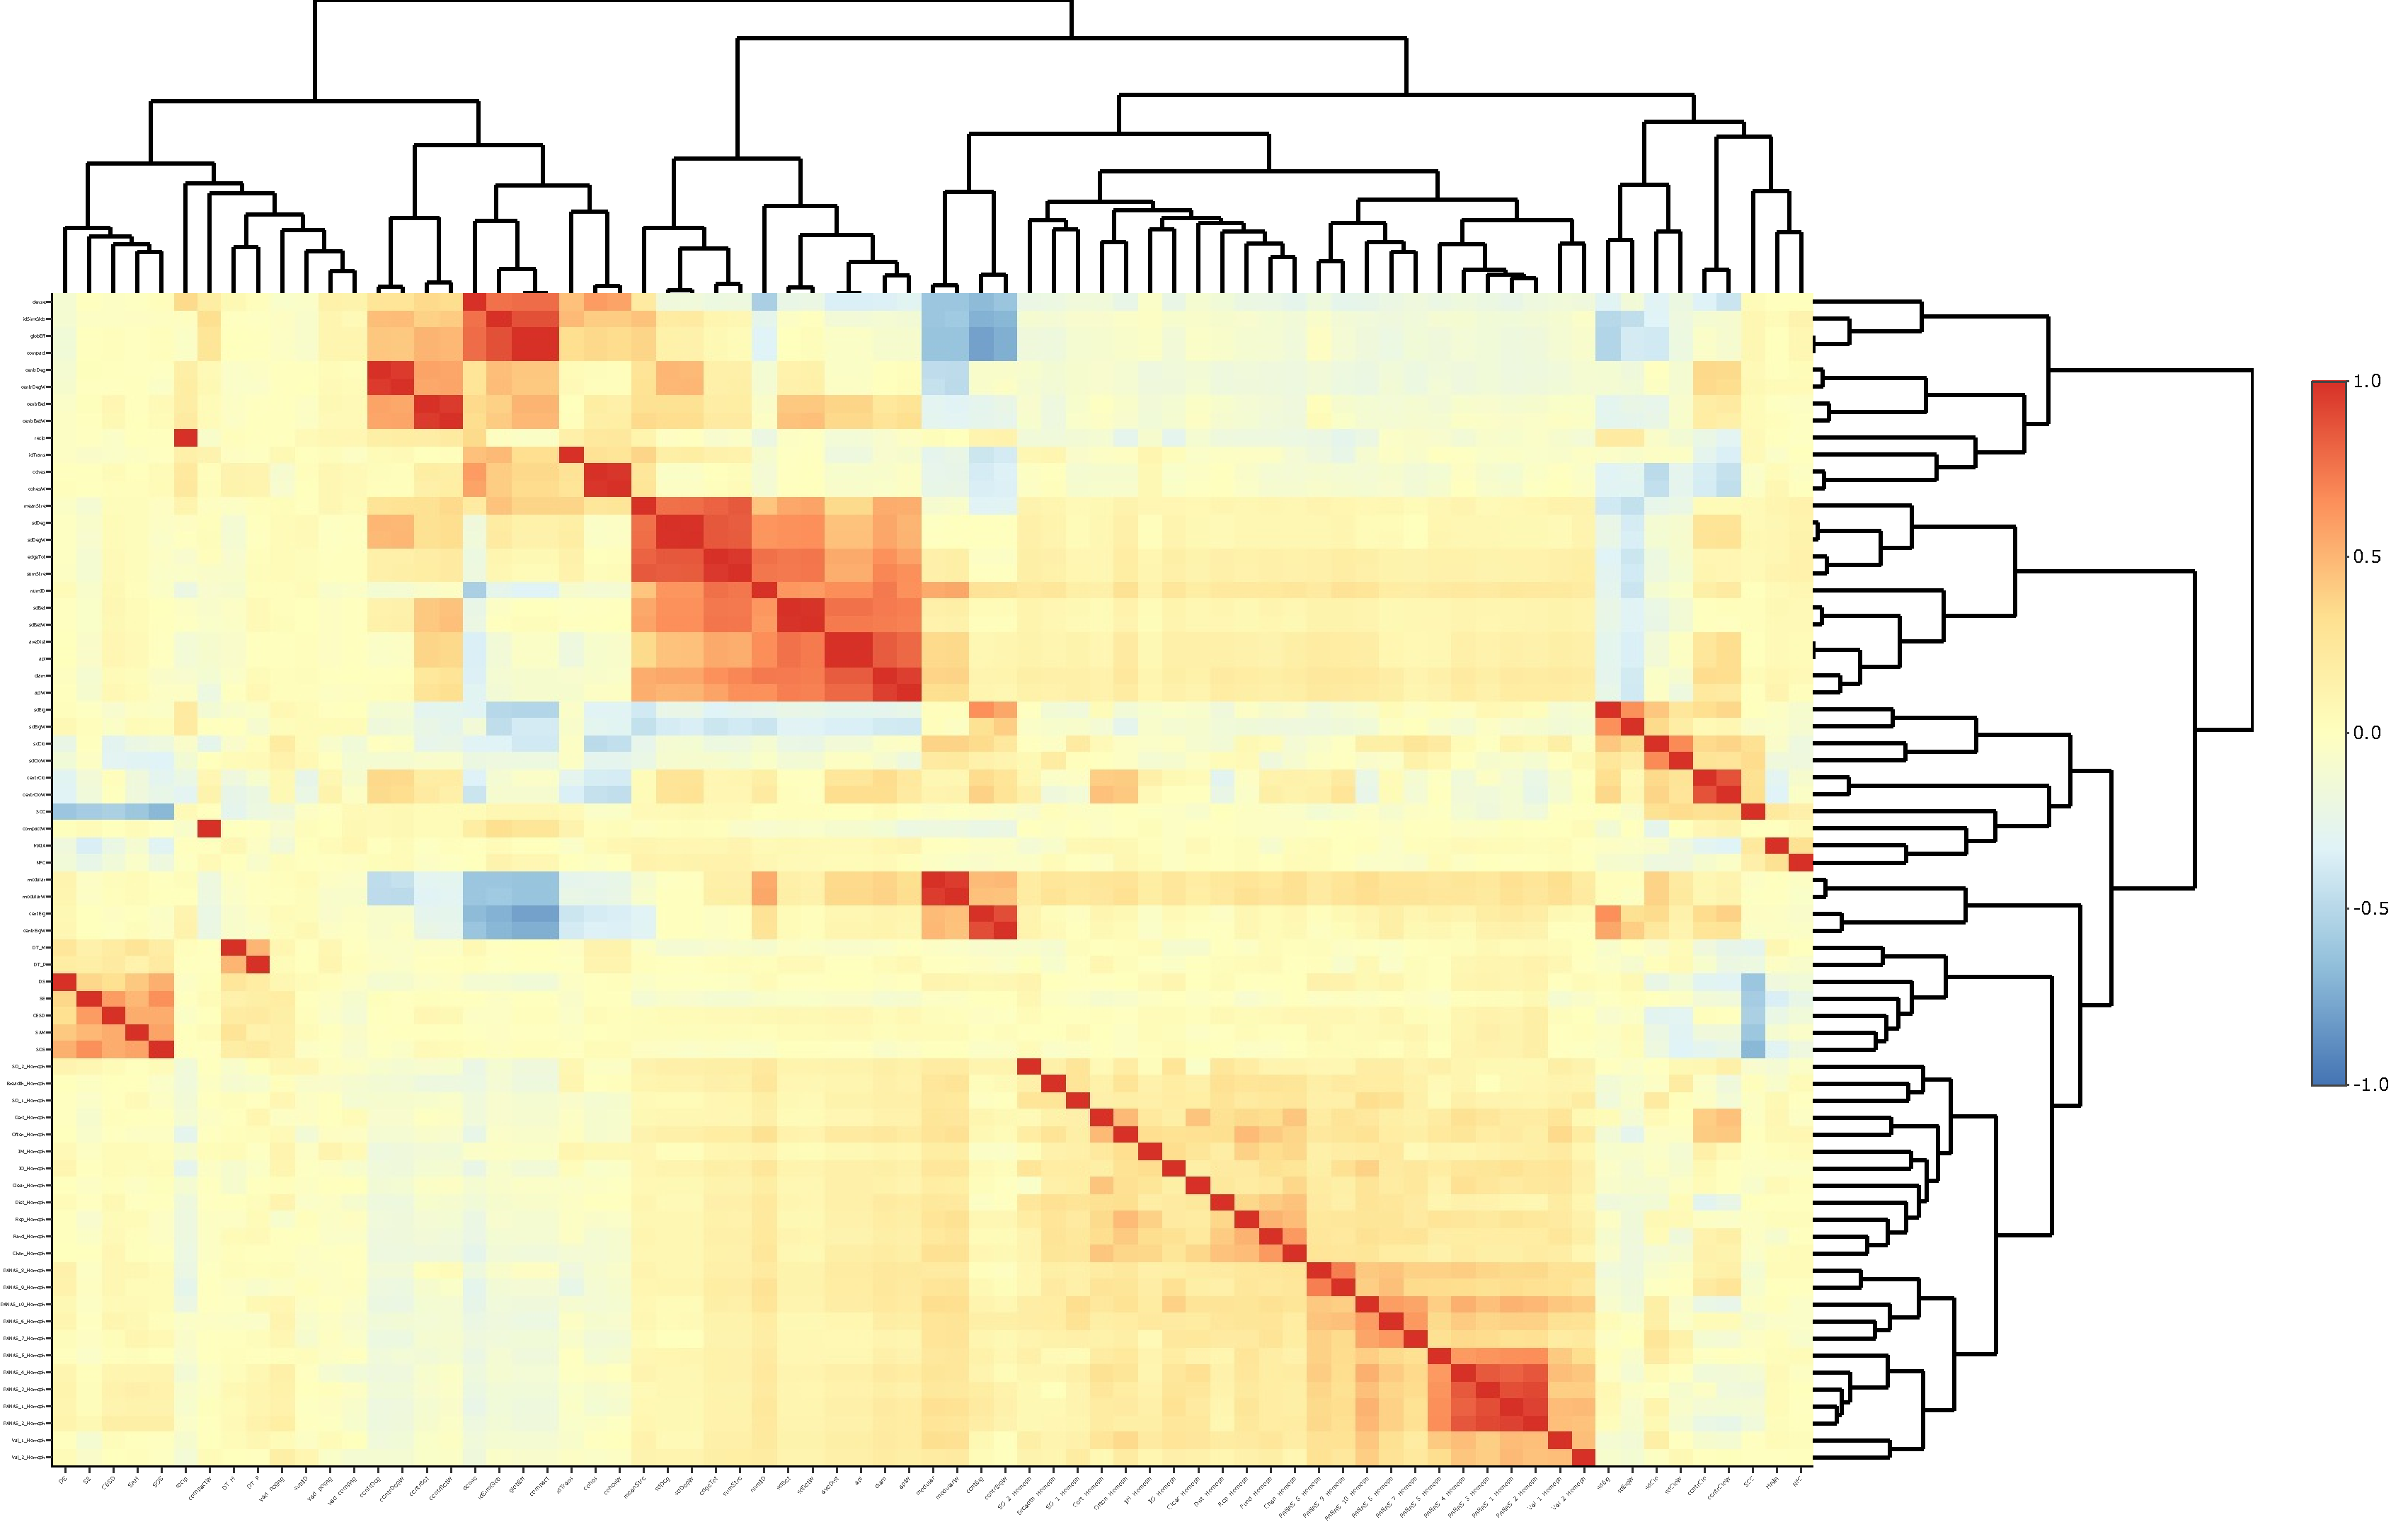
\includegraphics{EpMemNet_LabPres_htmldoc_files/figure-pdf/unnamed-chunk-69-1.pdf}

\hypertarget{summary}{%
\section{Summary}\label{summary}}

\hypertarget{recap}{%
\subsection{Recap}\label{recap}}

\begin{itemize}
\item
  Asymmetric stronger effects of implications relative to inward causes
\item
  Outward implications predicts how fundamental or important to change
  an experience was, how clearly defined/certain in memory one is, and
  how representative the experience is\ldots{}
\item
  Inward causes predict positivity (across self-report and positivity of
  text used) but not negativity
\item
  Superordinance: More outward implications, more broad\ldots{} Like
  foundation of a building, the most causal are the most broadward
\item
  Structurally similar memories share similar beliefs/attitudes towards
  them
\end{itemize}

\hypertarget{potential-criticisms}{%
\subsection{Potential Criticisms}\label{potential-criticisms}}

\begin{itemize}
\item
  There's a lot of inward and outward effects, even if inward is weaker.
  Is it \emph{really} directed?
\item
  Are these causal relations meaningful, or do people just ``click'' the
  memories that mean a lot to them more often?
\item
  Any others?
\end{itemize}

\hypertarget{pending-questions-for-study-2}{%
\subsection{Pending Questions for Study
2}\label{pending-questions-for-study-2}}

\begin{itemize}
\item
  How can we support this directed/causal representation of episodic
  memory?
\item
  How can we modify/augment episodic memories?
\item
  How can we support that more implications == more transformative?
\item
  How can we support that if memory did not exist, it's consequences
  would not either (i.e., counterfactual reasoning)?
\end{itemize}

\hypertarget{next-steps}{%
\section{Next Steps}\label{next-steps}}

\hypertarget{tweaksrephrasings}{%
\subsection{Tweaks/Rephrasings}\label{tweaksrephrasings}}

\begin{itemize}
\item
  Remove questions to reduce time (Which?)
\item
  For MTurk, fix episodic memories max at 15 rather than 30? Require 15
  to keep constant?
\item
  Pivot towards episodic memories/experiences person \textbf{chose} to
  have (per L.A. Paul framing)?
\item
  Rephrase weighted network question to: How certain are you that if X
  did not occur, Y would not? Or how responsible?\ldots{} Feels more
  concrete, in line with Gerstenberg et al.~work on counterfactual
  reasoning/causal structure
\end{itemize}

\hypertarget{new-questions}{%
\subsection{New Questions}\label{new-questions}}

\begin{itemize}
\item
  How surprising or unexpected the experience was?
\item
  Whether you knew what it was like to have this experience, prior to it
  having been experienced?
\item
  Whether you anticipated the consequences it would have, prior to
  having the experience?
\item
  To what extent were your preferences and values changed by this
  experience?
\item
  To what do your values/preferences after this experienc differ from
  your values and preferences before undergoing this experience?
\item
  Rank order the memories experiences that would be most disruptive to
  who you are if they did not exist:
\end{itemize}

\hypertarget{the-simulation-heuristic}{%
\subsection{The Simulation Heuristic}\label{the-simulation-heuristic}}

\begin{itemize}
\item
  ``Assessments of causality. To test whether event A caused event B, we
  may undo A in our mind, and observe whether B still occurs in the
  simulation. Simulation can also be used to test whether A markedly
  increased the propensity of B, perhaps even made B inevitable. We
  suggest that a test of causality by simulation is involved in examples
  such as''you know very well that they would have quarrelled even if
  she had not mentioned his mother.'' - Kahneman \& Tversky, 1981
\item
  Biased towards downhill/subtractive change, reducing surprising
  antecedents
\end{itemize}

\hypertarget{additive-subtractive-and-substitution-counteractuals}{%
\subsection{Additive, Subtractive, and Substitution
Counteractuals}\label{additive-subtractive-and-substitution-counteractuals}}

\begin{itemize}
\item
  A student fails a test\ldots{}

  \begin{itemize}
  \item
    \textbf{Uphill/Additive:} \ldots{} If only I had purchased study
    materials.
  \item
    \textbf{Downhill/Subtractive:} \ldots{} If only I hadn't gone out
    drinking with me mates the previous night.
  \item
    \textbf{Horizontal/Subsitution:} \ldots{} If only I had focused on
    the text instead of my lecture notes.
  \end{itemize}
\end{itemize}

\hypertarget{counteractual-reasoning-task}{%
\subsection{Counteractual Reasoning
Task}\label{counteractual-reasoning-task}}

\begin{itemize}
\item
  Gerstenberg et al., 2022 on sustaining causation (blocks causing other
  blocks to be supported) ask to predict which blocks would fall if the
  black one were removed (selection), how many of the blocks would fall
  (prediction), and how responsible the black block is for the red
  blocks staying on the table (responsibility).
\item
  https://cicl-stanford.github.io/mental\_jenga/interface/
\end{itemize}

\hypertarget{counterfactual-reasoning-task}{%
\subsection{Counterfactual Reasoning
Task}\label{counterfactual-reasoning-task}}

\begin{itemize}
\item
  Introduce noise to estimate responsibility judgment
\item
  What is noise for episodic memories though?
\end{itemize}

\hypertarget{section}{%
\subsection{\texorpdfstring{\protect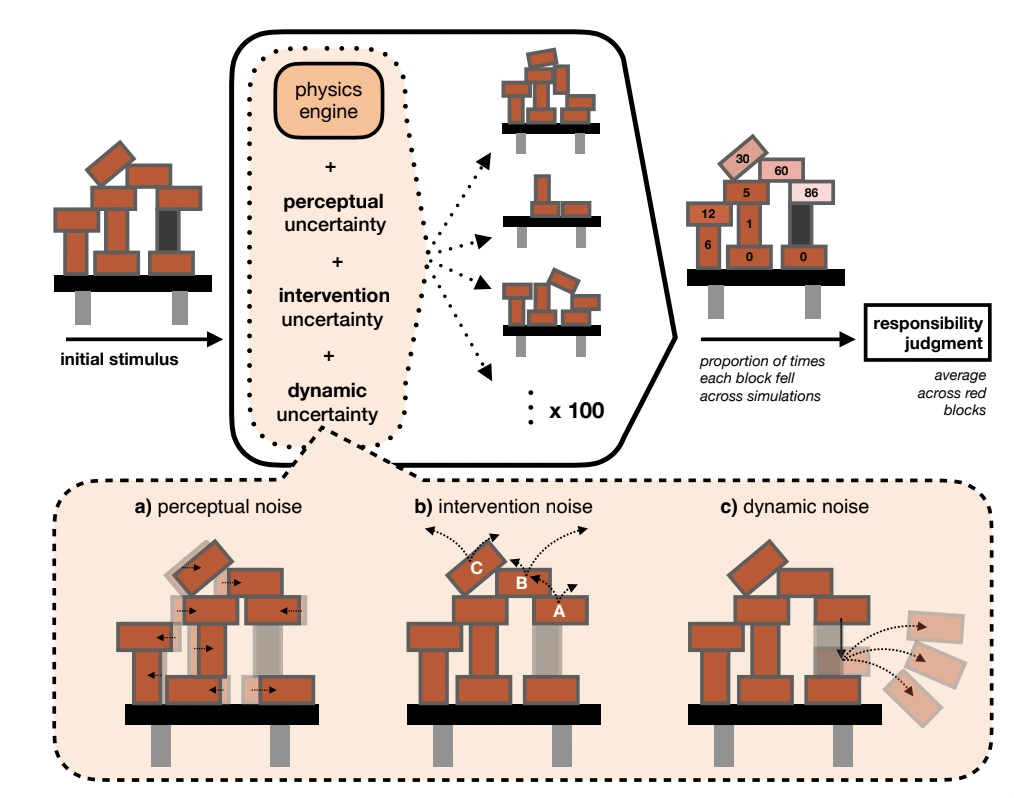
\includegraphics[width=5.375in,height=\textheight]{images/Screen Shot 2023-01-30 at 4.46.55 PM.png}}{}}\label{section}}

\hypertarget{counterfactual-reasoning-task-1}{%
\subsection{Counterfactual Reasoning
Task}\label{counterfactual-reasoning-task-1}}

\begin{itemize}
\item
  In the current work on our trait network work, we more or less
  implement the ``Selection'' condition.
\item
  Is there a way to implement ``Prediction'' and ``Responsibility''
  conditions?

  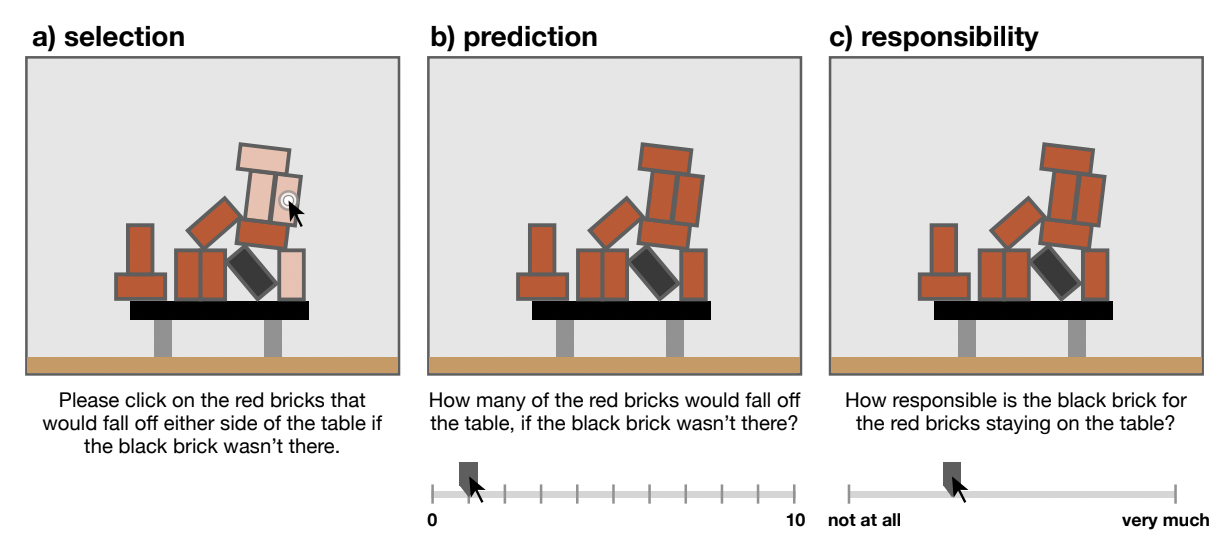
\includegraphics{images/Screen Shot 2023-01-30 at 4.48.53 PM.png}
\end{itemize}

\hypertarget{future-studies-if-i-had-time}{%
\subsection{Future Studies\ldots{} if I had time
:'(}\label{future-studies-if-i-had-time}}

\begin{itemize}
\item
  Some of strongest evidence for mental simulation models of
  counterfactual reasoning come from eye-tracking

  \begin{itemize}
  \tightlist
  \item
    People look at where B would have gone if it were not for A
  \end{itemize}
\item
  Collect data, generate networks, implement perturbations to network,
  and measure the extent to which participants predict instability
\end{itemize}



\end{document}
